\documentclass[12pt,english]{article}
\usepackage{preamble}
\newcommand{\macrotikz}{\documentclass[tikz]{standalone}
\usepackage{tikz}
\usepackage{pgfplots}
\pgfplotsset{compat=newest}
\usetikzlibrary{plotmarks}
\usetikzlibrary{arrows.meta}
\usepgfplotslibrary{patchplots}
\usepackage{grffile}
}

\begin{document}
\cleardoublepage
\pagenumbering{gobble}
%%%%%%%%%%%%%%%%%%%%%%%%%%%%%%%%%%%%%%%%%
% University Assignment Title Page 
% LaTeX Template
% Version 1.0 (27/12/12)
%
% This template has been downloaded from:
% http://www.LaTeXTemplates.com
%
% Original author:
% WikiBooks (http://en.wikibooks.org/wiki/LaTeX/Title_Creation)
%
% License:
% CC BY-NC-SA 3.0 (http://creativecommons.org/licenses/by-nc-sa/3.0/)
% 
% Instructions for using this template:
% This title page is capable of being compiled as is. This is not useful for 
% including it in another document. To do this, you have two options: 
%
% 1) Copy/paste everything between \begin{document} and \end{document} 
% starting at \begin{titlepage} and paste this into another LaTeX file where you 
% want your title page.
% OR
% 2) Remove everything outside the \begin{titlepage} and \end{titlepage} and 
% move this file to the same directory as the LaTeX file you wish to add it to. 
% Then add \input{./title_page_1.tex} to your LaTeX file where you want your
% title page.
%
%%%%%%%%%%%%%%%%%%%%%%%%%%%%%%%%%%%%%%%%%
%\title{Title page with logo}
%----------------------------------------------------------------------------------------
%   PACKAGES AND OTHER DOCUMENT CONFIGURATIONS
%----------------------------------------------------------------------------------------


\begin{titlepage}

\newcommand{\HRule}{\rule{\linewidth}{0.5mm}} % Defines a new command for the horizontal lines, change thickness here

\center % Center everything on the page

%----------------------------------------------------------------------------------------
%   LOGO SECTION
%----------------------------------------------------------------------------------------


\includegraphics[width=\textwidth]{fig/Logos}\\[2cm] % Include a department/university logo - this will require the graphicx package
 
%----------------------------------------------------------------------------------------
%   HEADING SECTIONS
%----------------------------------------------------------------------------------------

\textsc{\LARGE Brussels Faculty of Engineering}\\[1.5cm] % Name of your university/college
\textsc{\Large Modulation \& Coding}\\[0.5cm] % Major heading such as course name
\textsc{\large ELEC--H401}\\[0.5cm] % Minor heading such as course title

%----------------------------------------------------------------------------------------
%   TITLE SECTION
%----------------------------------------------------------------------------------------

\HRule \\[0.4cm]
{ \huge \bfseries Simulation of a DVB--S2 Communication Chain}\\[0.4cm] % Title of your document
\HRule \\[1.5cm]
 
%----------------------------------------------------------------------------------------
%   AUTHOR SECTION
%----------------------------------------------------------------------------------------

% If you don't want a supervisor, uncomment the two lines below and remove the section above
\Large \emph{Authors:}\\
Cédric~\textsc{Hannotier} \\% Your name
Badr-Ali~\textsc{Mouaden} \\
Mahtieu~\textsc{Petitjean}\\[2.5cm] % Your name

%----------------------------------------------------------------------------------------
%   DATE SECTION
%----------------------------------------------------------------------------------------

{\large \today}\\[2cm] % Date, change the \today to a set date if you want to be precise


%----------------------------------------------------------------------------------------

\vfill % Fill the rest of the page with whitespace

\end{titlepage}



\tableofcontents

\newpage
\cleardoublepage
\pagenumbering{arabic}

\section{Introduction}
This report presents the simulation of a DVB-S2 communication chain. The most important design parameters were varied in order to illustrate their impact on the quality of the communication via the bit error rate (BER).

This project was divided in three steps. Each of these steps is presented, then various graphs illustrate the important concepts and results. To conclude each section, questions regarding the simulation and the communication chain itself are answered.

\section{Optimal communication chain over the ideal channel}\label{sec:step1}
\subsection{Simulation}

The implementation scheme is shown in Figure \ref{fig:block}.

\begin{figure}[H]
    \centering
    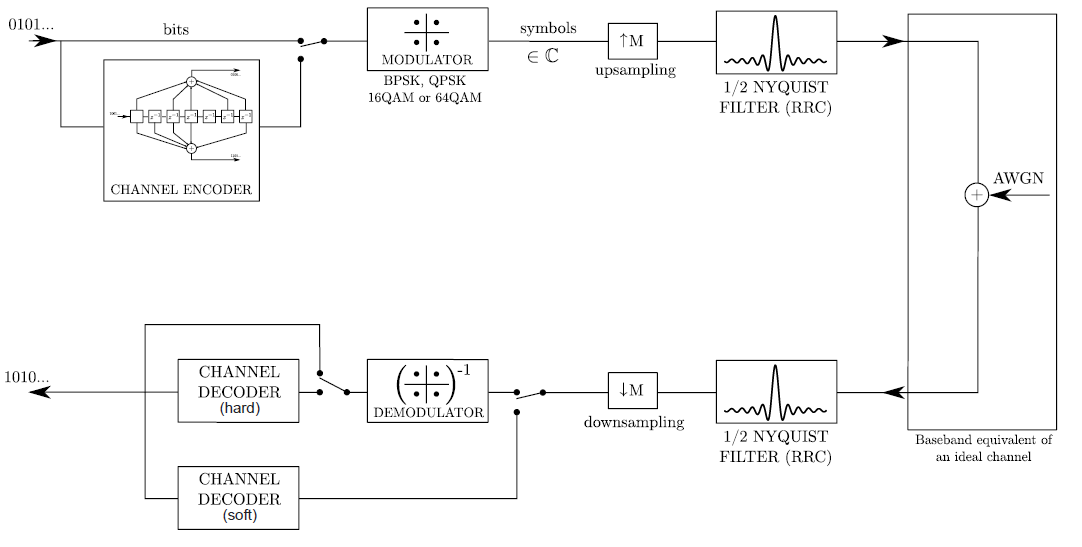
\includegraphics[width = .9\textwidth]{fig/block.png}
    \caption{Block scheme of the ideal channel}
    \label{fig:block}
\end{figure}

The various components of the communication chain are detailed hereafter. The channel encoder is not yet implemented, and the symbols mapping/demapping were provided.

\subsubsection{Halfroot Nyquist filter}

After the mapping, the complex symbols are convolved with a root raised-cosine filter. It allows to limit the communication bandwidth, as illustrated in Figure \ref{fig:filter} where the PSD of the symbol stream are shown before and after filtering, with a rolloff factor $\beta$ of $0.3$. The symbol frequency was fixed to 2 \si{\mega \hertz}, which translates to a cutoff frequency of 1 \si{\mega \hertz}.

\begin{figure}[H]
\centering
    \includegraphics{fig/filter.tex}
     \caption{PSD of the symbol stream at the transmitter before and after filtering}
    \label{fig:filter}
\end{figure}

At the receiver side, the stream is convolved again with the matched filter, forming a Nyquist filter and maximizing the SNR. The Nyquist filter allows to cancel the ISI in the sense that it reduces to a Dirac pulse when sampled at the symbol frequency, as shown in Figure \ref{fig:isi}. Hence, no symbol of the symbol stream overlaps with the current received symbol.

\begin{figure}[H]
\centering
    \includegraphics{fig/isi.tex}
     \caption{Illustration of the cancellation of ISI by the Nyquist halfroot filter}
    \label{fig:isi}
\end{figure}


\subsubsection{Noise addition}

The channel is corrupted by Additive White Gaussian Noise (AWGN), which is simulated using its baseband equivalent representation. The channel was simulated for various SNR (defined with respect to the bit energy) and various modulation schemes, and the results are plotted in Figure \ref{fig:ber}. The simulations confirm the theoretical results.


\begin{figure}[H]
\centering
    \includegraphics{fig/ber2.tex}
    \caption{Bit error rate as a function of the SNR for various modulations. The full lines correspond to the theoretical curves and the dots to the simulation.}
    \label{fig:ber}
\end{figure}

As expected, more energy is required to have the same BER when the constellation size is increased. It is worth noting that the worst BER value that could be achieved is 0.5, corresponding to a random choice of the binary values. Moreover, the BER curves for 2-PAM and 4-QAM are superposed because a 4-QAM modulation can be seen as two 2-PAM modulations in quadrature.



\newpage
\subsection{Questions}

\subsubsection{Questions regarding the simulation}

\paragraph{It is proposed to use the baseband equivalent model of the AWGN channel. Would it be possible to live with a bandpass implementation of the system ?} \mbox{}

The baseband model allows to implement the simulations regardless of the carrier frequency. If the system were simulated in bandpass, the required sampling frequency would be extremely high and unrealistic.

\paragraph{How do you choose the sample rate in Matlab ?} \mbox{}

The sampling rate should be at least twice as high as the symbol frequency. It will be increased further when simulating the sample time shift in the third step.

\paragraph{How do you make sure you simulated the desired $E_b/N_0$ ratio ?} \mbox{}

First the energy of a bit is evaluated, then the noise power is computed in order to obtain the desired $E_b/N_0$ ratio. The energy of the bit $E_b$ is given by

\begin{equation*}
    E_b = \frac{T_{samp}}{2 N_{bits}} \sum_{n} {\left| s \left[ n \right] \right|}^2
\end{equation*}

Then $N_0$ can be chosen according to the wanted SNR and the noise is added to the symbols using the baseband representation :

\begin{equation*}
    r \left[ k \right] = \sqrt{N_0 f_{samp}} \left\{ \mathcal{N}(0,1) + j \mathcal{N}(0,1) \right\}  
\end{equation*}

The square root is present because of the baseband representation of the noise. Indeed, the computed power is equally distributed between the real and imaginary parts of the noise.

\paragraph{How do you choose the number of transmitted data packets and their length ?} \mbox{}

A rule of thumb is to send $10^{n+2}$ bits of data in order to reliably observe of BER of $10^{-n}$ as it corresponds to 100 detected errors. Moreover, the total number of bits should be a multiple of the number of bits per symbol used in the modulation scheme. The Figure \ref{fig:ber} was realised by sending around $10^8$ bits of data.

\subsubsection{Questions regarding the communication system}

\paragraph{Determine the supported (uncoded) bit rate as a function of the physical bandwidth.} \mbox{}

The bit rate $R$ is given by $R = \frac{log_2 (M)}{T}$ where $M$ is the number of symbols and $T$ is the symbol duration. The Nyquist filtering yields a relationship between the symbol duration and the bandwidth, $\Delta f = 2/T$ (this can be seen on Figure \ref{fig:filter} where T = 0.5 \si{\micro \second} and $\Delta f = 2$ \si{\mega \hertz}). This gives:

\begin{equation*}
    R = \frac{log_2 (M) \ \Delta f}{2}
\end{equation*}

\paragraph{Explain the trade-off communication capacity/reliability achieved by varying the constellation size.} \mbox{}

As detailed in the previous question, increasing the constellation size (the number of bits transmitted per symbol $M$) allows to increase the bit rate. However, the minimum euclidean distance between the symbols in the constellation size decreases, which causes the error probability to increase. As a result, to achieve a similar BER, more energy is required when the constellation size increases but the bit rate also increases.

\paragraph{Why do we choose the halfroot Nyquist filter to shape the complex symbols ?} \mbox{}

The halfroot Nyquist filter allows to limit the communication bandwidth (it is more spectrally efficient than the plain rectangular window) and allows to cancel ISI.

\paragraph{How do we implement the optimal demodulator? Give the optimization criterion.} \mbox{}

The optimal demodulator is implemented 	as a bank of K filters matched to the basis functions of the modulation scheme: 

\begin{equation*}
	h_i(t) := s_i(-t) \hspace{1cm}  i=1,...,K
\end{equation*}

The outputs to such filters are the autocorrelations between the input signal and the basis functions. The filters are mathematically equivalent to a bank of K correlators. The optimisation criterion is the maximisation of the SNR at the output. It is realized by the matched filters, and the SNR will be equal to $\frac{2\mathcal{E}}{N_0}$.

\paragraph{How do we implement the optimal detector? Give the optimization criterion.} \mbox{}

There exist two possible optimization criteria for the detector. First, the maximum a posteriori (MAP) criterion, which minimises the error probability by exploiting the knowledge of the a priori probabilities $p(\underline{s}_m)$ and the conditional probabilities $p(\underline{r}|\underline{s}_m)$, where $\underline{r}$ is the observation. It selects the symbol which is the most likely to have been sent, knowing that we observed $\underline{r}$.
	
	\begin{equation*}
		\underline{\tilde{s}}^{\text{MAP}}_m = \underset{\underline{s}_m}{\text{max}} \ p(\underline{s}_m |\underline{r}) \stackrel{\text{Bayes}}{=}
		\underset{\underline{s}_m}{\text{max}} \ p(\underline{r} |\underline{s}_m) p(\underline{s}_m)
	\end{equation*}
	
The maximum likelihood criterion is equivalent to the MAP criterion when all the M symbols are equally probable, so that $p(\underline{s}_m) = 1/M$ is constant and can be dropped when maximizing the probabilities.
	
	\begin{equation*}
		\underline{\tilde{s}}^{\text{ML}}_m = \underset{\underline{s}_m}{\text{max}} \ p(\underline{r} |\underline{s}_m) 
	\end{equation*}
	
The ML criterion determines what symbol is the most likely to have produced the received signal by selecting the symbol which has the lowest euclidean distance to the received symbol.



\section{Low-density parity check code}
\subsection{Simulation}

The channel encoder that was skipped in section \ref{sec:step1} is now implemented as a low-density parity check code (LDPC) encoder. Soft and hard decoding have been implemented with a code rate of 1/2 and their performance is compared next.

The channel coding adds structured redundancy  to the information sent by the transmitter to be able to detect and correct errors at the receiver side. The LDPC code has the property that the check matrix is sparse, allowing a lower complexity of the implementation.

\subsubsection{Hard decoding}
\iffalse
\begin{figure}[H]
\centering
    \includegraphics{fig/HardLDPC.tex}
     \caption{Hard LDPC}
    \label{fig:HardLDPC}
\end{figure}
\fi

The hard decoding is based on the implementation of a Tanner graph. The influence of the maximal number of iterations on the BER curves is shown in Figure \ref{fig:HardLDPCbis} for a 16-QAM modulation. The conclusions can be generalized to any modulation.

\begin{figure}[H]
\centering
    \includegraphics[width=\textwidth]{fig/HardLDPCbis.tex}
     \caption{Effect on the BER curves of Hard LDPC decoding for a 16-QAM modulation}
    \label{fig:HardLDPCbis}
\end{figure}

For the hard decoding, the performance is worsened at low SNR. Indeed, a noise which is too important causes the code to add errors when it is trying to correct them. Increasing the maximal number of iterations allows a slight improvement in performance.

\subsubsection{Soft decoding}

In practice, hard decoding is never used as the soft decoding allows for much better performance. Instead on basing the decision on the received bits, it computes probablities based on the received symbols. The results of the simulations for a 2-PAM is shown in Figure \ref{fig:SoftLDPC}.

\begin{figure}[H]
\centering
    \includegraphics{fig/SoftLDPC.tex}
     \caption{Effect on the BER curves of Hard LDPC decoding for a 16-QAM modulation}
    \label{fig:SoftLDPC}
\end{figure}

The theoretical curve for the ideal communication chain as well as the curve for hard decoding are shown as references. The improvement is significant with soft decoding.

\subsection{Questions}

\subsubsection{Questions regarding the simulation}

\paragraph{When building the new BER curves, do you consider the uncoded or coded bit energy on	the x-axis?} \mbox{}

The coded bit energy is considered here.

\paragraph{How do you limit the number of decoder iterations?} \mbox{}

For the hard decoding, the iterations stop either when the maximum number of iterations is reached or when the syndrome is zero.

For the soft decoding,  stop either when the maximum number of iterations is reached or when there is no more detected errors.

\paragraph{Why is it much simpler to implement the soft decoder for BPSK or QPSK than for 16-QAM or 64-QAM?} \mbox{}

In the case of the 16-QAM or 64-QAM, the euclidean distance should be computed when decoding. This is not the case for BPSK and QPSK, where the decision can be made only by looking at the real and imaginary part of the received symbols.

\subsubsection{Questions regarding the communication system}

\paragraph{Demonstrate analytically that the parity check matrix is easily deduced from the generator matrix when the code is systematic.} \mbox{}

A code is systematic when the mapping is such that part of the code vector coincides with the message vector. In that case, the generator matrix has the form $\underline{\underline{G}} = \left[\underline{\underline{P}} | \underline{\underline{I}}\right]$, with $\underline{\underline{P}}$ the parity array and $\underline{\underline{I}}$ the identity matrix of the corresponding size.
The parity check matrix should be created so that its rows are orthogonal to the rows of the generator matrix:

\begin{equation*}
 \underline{\underline{G}} \cdot \underline{\underline{H}}^T = \underline{\underline{0}}
\end{equation*}

The solution to this equation is given by $\underline{\underline{H}} = \left[\underline{\underline{I}} | \underline{\underline{P}}^T\right]$. Indeed:

\begin{equation*}
	\underline{\underline{G}} \cdot \underline{\underline{H}}^T = \left[\underline{\underline{P}} | \underline{\underline{I}}\right] \cdot \left[\underline{\underline{I}} | \underline{\underline{P}}^T\right]^T =  \underline{\underline{P}} \oplus  \underline{\underline{P}} =0
\end{equation*}

\paragraph{Explain why we can apply linear combinations on the rows of the parity check matrix to produce an equivalent systematic code.} \mbox{}

The rows of the parity check matrix are the basis vectors of a subspace which is perpendicular to the subspace spanned by the generator matrix. A linear combination of these basis vectors will still be a basis for the same subspace and the resulting code will be equivalent.

\paragraph{Why is it especially important to have a sparse parity check matrix (even more important	than having a sparse generator matrix)?} \mbox{}

A sparse parity check matrix allows to significantly reduce the complexity of the decoder. Indeed, element $H_{ij}$ being equal to 1 results in a logical connection in the Tanner graph between the check-node $c_i$ and the variable-node $v_j$. Hence, reducing the number of 1's in $\underline{\underline{H}}$ reduces the number of exchanged messages and the number of computations.

\paragraph{Explain why the check nodes only use the information received from the other variable nodes when they reply to a variable node.} \mbox{}

The information exchanged between the check and variable nodes has to be statistically independent for hard and soft decoding. This means that only the information which is not related to the current node is used to compute the answer.

\section{Time and frequency synchronisation}
\subsection{Simulation}
In this section, the synchronisation errors caused by the hardware, the carrier phase and frequency shift are simulated, then algorithms allowing to reduce them are introduced.

\subsubsection{Synchronisation errors}

On \autoref{fig:CFOphi} is shown how the CFO affects the constellation. The linearly increasing phase shift caused by the CFO causes a rotation of the symbols. This effect is first manually corrected to study the impact of ISI only.

\begin{figure}[H]
    \centering
    % This file was created by matlab2tikz.
%
%The latest updates can be retrieved from
%  http://www.mathworks.com/matlabcentral/fileexchange/22022-matlab2tikz-matlab2tikz
%where you can also make suggestions and rate matlab2tikz.
%
\definecolor{mycolor1}{rgb}{0.00000,0.44700,0.74100}%
\definecolor{mycolor2}{rgb}{0.85000,0.32500,0.09800}%
\definecolor{mycolor3}{rgb}{0.92900,0.69400,0.12500}%
%
\begin{tikzpicture}

\begin{axis}[%
width=10.624in,
height=5.824in,
at={(1.782in,0.786in)},
scale only axis,
xmin=-2,
xmax=2,
ymin=-2.00266591089304,
ymax=2,
axis background/.style={fill=white},
title style={font=\bfseries},
title={EbN0 = 6 dB and phi = pi/4},
legend style={legend cell align=left, align=left, draw=white!15!black}
]
\addplot [color=mycolor1, draw=none, mark=x, mark options={solid, mycolor1}]
  table[row sep=crcr]{%
0.707106781186547	-0.707106781186547\\
-0.707106781186547	-0.707106781186547\\
-0.707106781186547	0.707106781186547\\
0.707106781186547	0.707106781186547\\
-0.707106781186547	-0.707106781186547\\
};
\addlegendentry{Emitted symbols}

\addplot [color=mycolor2, draw=none, mark=o, mark options={solid, mycolor2}, forget plot]
  table[row sep=crcr]{%
0.675233106584623	-0.744419448532486\\
-0.636921205126137	-0.835265882002788\\
-0.689817677947621	-0.718342889960331\\
-0.583501550498548	0.892451201521953\\
-0.298345780147174	0.475109465875956\\
-0.0104868838585701	-0.877956587033837\\
-1.26687156893945	0.453181902940008\\
0.720169102027316	0.684898453152319\\
0.771624710760068	1.14279300097057\\
-0.721140703957037	-0.443355483432679\\
-0.98958845118541	-1.0321528346279\\
0.481356517831017	0.560938717337793\\
0.60693959330412	1.02531167881519\\
-0.736265139834899	0.822583796647838\\
-0.986679140892251	-0.290758015298934\\
0.494635002791912	1.10384472600927\\
-1.02568278241804	-0.424237895144064\\
-0.384101411427955	-0.401863971299114\\
-0.718783226600815	0.646327975823159\\
0.517716155689898	0.537474289459519\\
-0.164364250946755	-0.522205275171892\\
-0.776676199520084	-0.550057148403217\\
0.886258073203444	0.814390954036338\\
0.494282353926119	-0.956316151001514\\
-0.963087063401344	1.12157369751279\\
0.651875239226979	-0.711540418814942\\
0.981507089606158	1.05225035935009\\
-0.617017536897364	0.45217267506038\\
0.577190020000684	0.940904149111001\\
0.334862028814832	-0.836660148088224\\
0.827182406297468	0.506152567643163\\
-0.679775958618497	-0.97851067198101\\
-0.932311402759095	-0.461366745159782\\
-0.531989268689352	0.649482313694433\\
0.751502630568312	-0.544670468549332\\
-0.894659513419118	1.15713937700438\\
-0.878152838051534	-0.956292284827014\\
0.416846695656121	0.440557890409285\\
-0.628384058180804	-0.770477524076566\\
-1.5658076153631	0.960195536667986\\
0.731196564497491	0.665720304446774\\
-0.978199296434623	-0.440145229632895\\
0.839696464953994	-0.783773090182678\\
-1.01232280706089	-0.919221040189415\\
0.444016316784323	-1.0571758771804\\
-0.787760546564511	0.829375050796106\\
0.366522671365173	0.843460224709192\\
0.783137693829913	0.572210218976281\\
0.665837452270529	0.399877601736522\\
-0.35920113372235	-0.895116043472054\\
0.617031391836399	0.804240130076769\\
-0.749009518823987	0.559217616458107\\
-0.715773894917881	0.657074717922653\\
-0.894355271838737	0.505441293590262\\
0.505758829040075	0.29146252107113\\
0.621891622684233	-0.906551043237634\\
-0.76761136750338	-0.434253393474188\\
-1.0318183436515	0.35150588207393\\
1.16579807192571	-0.402657951206969\\
-0.687132814664683	0.516849561446372\\
-0.724359532998173	0.62907439137792\\
-0.672044421385474	-0.4535815201206\\
-1.12330861502927	0.458147852506172\\
-0.59476321920246	0.758058638114172\\
0.91170013083573	0.998399324629698\\
0.691568993788721	-0.732646038662022\\
1.03120434797173	-0.351255663851726\\
-0.420865559565061	1.03882786863572\\
-0.332168422398352	0.364751254706802\\
1.38975157463443	-0.713416424699647\\
-0.97866681705727	0.4094241451595\\
-0.886622128273773	1.08266842508607\\
0.844320020092694	0.74176931205898\\
0.554438256137929	0.671306282345577\\
1.02511109597404	-0.740536258095758\\
-0.620571608679077	-0.57325593739933\\
0.752670505574199	-1.11939921627418\\
0.964540225971935	-0.825016499996293\\
0.783094794352488	-0.397509556481649\\
-0.82284484041336	0.686910289840411\\
0.642894817380335	0.627632393272583\\
-0.603246017402051	-0.932933622206857\\
-0.995004109693025	1.12689501454592\\
-0.779655437512219	1.21075073229633\\
1.0568653840325	0.795013158538588\\
-0.416565668849779	0.478677483245065\\
1.00432412214953	-0.98740347371109\\
-0.880706661635706	-0.515944317711307\\
0.652000398106523	1.42507590951922\\
-1.05540630839214	-0.845571666204369\\
-0.687972335439113	-0.391134072335554\\
-0.512033516423268	-0.505300885653547\\
1.01090005633488	0.644168803976666\\
0.943502590704546	0.648444551710609\\
-0.636913022342505	-0.772005599318889\\
-0.656629646824704	-0.791763618503587\\
0.670264455793958	-0.867787945240849\\
-0.471633385140731	0.615070664096101\\
-0.684390857332859	-0.419988662088858\\
-0.709332786796703	-0.300318503855041\\
-0.257940899078633	0.221966742698579\\
-0.443786552720326	0.80889028782244\\
0.836418143349224	0.938526202936364\\
0.900585019535358	0.279863016450462\\
-0.730881014040438	-0.638391212016451\\
0.475780379674726	-0.626568878632406\\
-0.425414573137613	-0.768257334397469\\
0.373967453577289	0.579543878441798\\
1.07537010491616	-0.542043336238569\\
-0.992190661830143	-0.50170102393404\\
0.530949949797556	-0.558978378001047\\
-0.485685885504384	0.512737600441231\\
-0.709743798945488	-0.650341147196151\\
-1.22055533429205	-0.733639724250386\\
-1.04058306843837	0.528268792374817\\
0.827886093256831	1.02434095614448\\
-0.524119657298818	0.674766889284822\\
-0.417296070855874	-0.808966622090996\\
0.650105528705358	-0.866666779489772\\
-0.67296394239093	0.556771129814855\\
1.28048385283739	0.823899340767698\\
-0.689337689170335	1.03876087559107\\
0.514059177491407	0.987590322823586\\
0.882036776154594	-0.678652484398305\\
0.858135275788436	-0.980067617856973\\
-0.574259234296288	1.232045908458\\
-0.816876512124798	0.855198521991454\\
-1.01438906765959	-0.589782711546637\\
-0.720536006514332	-0.651183772856487\\
0.762033224603234	0.696580294459419\\
0.425060516825882	0.700157995496944\\
-0.692539493246121	-0.772369508373645\\
-0.351711462250685	-0.800028477105681\\
0.727183940239755	0.827204970196274\\
0.3063190067108	0.750020367110048\\
-0.36346463462608	-0.924907696536514\\
-0.497693623709013	-0.764277002909693\\
-1.2488839099608	-0.946880689395857\\
-0.926101374844616	-1.25836961619345\\
-0.885814035473171	-0.993400074511867\\
0.895799540968371	-0.652225679500694\\
-0.511606147958335	-0.799068692474066\\
0.711314635204279	-1.19314944920235\\
0.461959762716015	0.680639642431449\\
0.696353463396407	-1.02790381129609\\
0.522969179903543	0.602465587111615\\
0.639244407882873	0.58806226870024\\
0.915723776201991	-0.771011825116781\\
-0.44902605927946	-1.09122357033551\\
1.01955616189377	-0.66887263957745\\
-0.339427840961799	0.917677076693573\\
-0.791905514384537	0.910520191086161\\
0.733118873926573	-0.536100636109797\\
-1.11725795645535	-0.612561069793268\\
0.654033008044861	0.779143022369229\\
-0.796291383468947	0.635339096364953\\
-0.67059355114295	-1.13606931605329\\
0.553300885847743	1.01988426437571\\
0.417420157833696	0.924000730591657\\
-0.884866207144275	-0.623159753864444\\
0.874620798311414	-0.470336355419207\\
-0.711267065365102	0.577109042174903\\
0.878930328783155	0.766614627076638\\
0.48111393428838	0.724416210369173\\
-0.720085826360561	0.704089019277226\\
-0.789044832322352	-0.717393027972659\\
-0.834545396234537	0.386938867433967\\
0.697350086204555	0.926786332755961\\
0.604679367349398	0.609982542460866\\
-1.19890182299201	-0.623397134916513\\
-0.340943815316143	0.522502717503963\\
-0.938664399239782	-0.497180031355499\\
-1.02050650708902	-0.597112461123355\\
-0.913605434971012	0.915215965092203\\
0.59962048112448	0.725738699253882\\
0.641366212666086	0.591146637312457\\
1.06317342991643	0.623531683380867\\
0.152803506423447	-0.880957099274575\\
-1.27138475726594	-1.17319934223976\\
0.926025315078062	-0.674619305151109\\
-0.716230744682676	-1.01640893480125\\
0.797345541325746	-0.745926061936523\\
0.110314749149561	-0.551172443020447\\
-0.311985002418946	-0.916188168045359\\
0.705037619060712	0.739913251004203\\
0.57215002595862	-0.52762507056606\\
-0.991053469783282	-0.905679772873362\\
0.857119642608703	-0.612385173213357\\
0.549136865380549	-0.82262204619275\\
-0.400039106440572	-0.641475575862104\\
-0.558587937974357	-1.1460879316691\\
0.482028060501607	0.736140729042313\\
-0.366066555090992	0.999885240363981\\
-0.562559617220958	-0.260442223931492\\
-0.899406561691665	0.66275274874309\\
0.645158979412821	0.780886789333264\\
0.792269113379192	-0.671308733835405\\
0.727568281776059	-0.647196159950543\\
0.778761659290771	0.764157355207133\\
0.282635797883409	0.441105810268095\\
0.841754240039514	-0.258645995081852\\
0.681233195603211	0.791851537290372\\
-0.805426112800932	-1.08918761043102\\
-0.895036002177897	-1.01993833420908\\
0.619332501979768	1.35990019789533\\
-0.72566809135422	-0.910509855283999\\
0.903751330524017	0.746814280078197\\
1.38514362001824	0.755248812541049\\
0.528820917607266	-1.08724957796104\\
-0.336135999390187	-0.19553383801022\\
-0.648276230307479	0.706923598707654\\
0.645465747299498	-0.690438675807877\\
1.10349273050618	0.360032880160251\\
0.430294255708417	-0.44777243055151\\
-0.60215962041466	0.634539005713594\\
-1.09171713442302	-1.65594046806454\\
0.636849702524757	1.03796661058402\\
-1.32012565037882	-0.524091068723238\\
-0.999221183573712	-0.349368285378203\\
-0.606518055383923	-0.774350368455247\\
-0.0973766392172084	0.641557211712155\\
-1.07607080249141	-0.83870276972648\\
0.485564538341493	-0.600255840096663\\
0.696680638152798	-0.129091662608179\\
0.549889950519343	0.766341400695107\\
-0.266176049680739	-0.635221041533322\\
0.682881238331783	-0.370331920955864\\
0.835231718923061	0.6928866730339\\
-0.702136254876032	0.567510276451421\\
-1.12379904750331	1.01542973768282\\
-0.842257207737195	-0.676805014157063\\
-0.586569737417437	-0.618918605778146\\
0.335194719778247	0.873044216578802\\
-0.432701546874783	0.629193767221377\\
0.392390703391383	-0.55846708521957\\
-0.477772838044464	0.505493371553911\\
1.15545212009985	-0.681174271339425\\
-0.778016224663642	1.40425035852395\\
0.461533058951634	0.690945960533978\\
0.613845854871591	0.484848505594279\\
-0.887719691559776	0.941774973407071\\
0.69689726211421	0.779556676712071\\
1.00435291506932	-0.685583493394407\\
-0.744209964050251	-0.720479982474797\\
0.607173136538876	-0.727879537299374\\
-0.554220802917698	0.891980051537973\\
0.311399606863365	1.04630978627403\\
0.56948219504357	0.738336827489914\\
-0.767187364393646	-0.535568205462308\\
-0.186810837219257	-0.907632111820136\\
-0.647307680070114	0.326280180619949\\
-0.878781792669071	0.383383963074477\\
0.346669223497538	0.730338664793948\\
0.959305784163476	0.960182456419155\\
0.274530701357414	0.356866337260962\\
-1.00552387717117	-0.818021923587838\\
0.181596753985102	-0.728155248237069\\
-0.484238015292215	-0.804511719687985\\
-1.36225310989477	-0.7936369308589\\
0.953574337452775	0.865904610111784\\
-0.93995702466892	-0.561386118718674\\
-0.282939920715031	-0.691531021276642\\
0.479892375267384	-0.627285273926468\\
-0.825406368036152	0.704645420825614\\
0.531262507146159	-1.15879801255492\\
0.602608306143684	1.09159613572551\\
-0.704261091606745	-0.634811078321411\\
0.546910472273283	-0.621247985799769\\
-0.752780056650261	1.06337612036476\\
-0.496808061614595	-0.645842417230538\\
0.751966449318371	1.02307838687441\\
-1.14406524830434	0.980166636187157\\
0.569412660620833	-0.916429477475597\\
0.0470465042622155	0.312695442175422\\
-0.992172876993829	-0.911771721323142\\
-0.659547049380786	-0.682729594370443\\
0.577166960808783	0.595211941301205\\
-0.563135918896387	-0.78169358767721\\
-0.413362826031564	0.619277580786745\\
-0.510059343929126	-0.959295811578227\\
-0.948749040637409	-0.793965414634207\\
1.00579258810495	-0.194780809079676\\
0.728253656260098	1.06068974246316\\
-0.734945159997116	-0.926734265801844\\
0.694989313306449	0.436469471795097\\
-0.234235248064783	0.84492599208267\\
0.407412689933057	-0.691608760602999\\
-0.558709085934983	0.675110329485701\\
-0.758069712318812	-0.50913983920398\\
0.971672948039925	-0.601591407787726\\
-0.47961483929209	-0.346364586064914\\
-0.939723082683973	0.674781046915185\\
0.673670285708555	0.307916955888714\\
0.706186313261898	0.752706026974152\\
0.720699158064143	-0.541581583031383\\
-0.453709249581947	0.869785381054332\\
-0.938368674533022	0.297542274219545\\
0.248938609069623	0.780770368545934\\
-0.570027362498318	0.520196748487069\\
0.729121790387739	0.448275857444967\\
0.667774349598757	1.0781070589123\\
-0.800341479950813	0.654154419768563\\
0.375179342477844	-0.817582196584415\\
-0.454205118407195	0.573422495950258\\
-1.19229942737095	-0.744445393873419\\
-0.561359721726389	-0.529070481354776\\
-0.1582201014616	-0.697885338121824\\
0.832391840218612	1.26222614941652\\
0.898174873587508	0.615358523193577\\
0.673749918412507	0.741759879658009\\
0.428921858650603	0.567367299849155\\
-0.515356122442456	-0.749537537688289\\
-0.449722472094128	-0.670194045804128\\
-0.812692570581431	0.440320346119344\\
-1.05189220338165	-0.635334968297354\\
0.751343772763575	0.595011926325906\\
-0.482132417751329	0.586549048603757\\
0.880161424985834	0.619168108908365\\
0.949706834228508	-0.739288077803961\\
0.942028242711725	-0.902672095837113\\
-1.15865713353834	-0.846215617643594\\
0.395382622493678	-0.316220792108653\\
-0.814727206986004	-0.420058174663003\\
-1.23947433709355	0.727488914002994\\
-0.620241801262498	-1.19808185267898\\
0.55876274453543	-1.0012107784682\\
-0.956471759549178	0.536898636642302\\
1.06162334864239	0.769364436520944\\
0.863570121506477	0.955791440473278\\
0.693726446101251	-0.664017455593004\\
0.373996779665772	0.742076599016007\\
0.736832324873818	0.509393533077532\\
-0.845549608394131	0.426574178321129\\
-0.443547558776739	0.502924956718448\\
-1.25417308371406	1.17952578393868\\
0.948972628250228	-0.811646151179732\\
0.608897335378067	0.597604703222317\\
-0.822851299785928	0.584662643220914\\
-0.352116406829111	0.632049456637391\\
-1.02512029395441	-0.763908164163879\\
-0.43639612316693	0.727443805789668\\
-0.739410184076254	0.397163933427156\\
-0.840470350984472	-0.400427741275706\\
-0.741180806868636	0.70496180866038\\
-1.10720224242706	-0.800842229004267\\
-0.610820804938965	0.674050040234928\\
-0.687044502733725	0.843173952597547\\
-1.01660621580907	0.667436683756212\\
-0.903438044871295	-0.850795343036802\\
-0.534881275081412	-0.384425837713091\\
0.369584372595162	-0.88284541236409\\
-0.200911785045133	0.387135110689989\\
-0.94648907515311	0.373475145403979\\
-0.51450004193744	0.912910907350621\\
0.888176535656401	-0.440563154316282\\
0.59310116398672	0.839813847403352\\
0.934639285382064	0.7675538857185\\
-0.767142632316625	0.526340408438993\\
0.94151555609038	0.688083195125171\\
0.699474464962752	0.717269260658098\\
-0.667753122857148	-0.724906730102236\\
-0.916095172679823	0.977073009776296\\
0.764176178846397	-0.233529518571224\\
-0.403956753214632	-0.83644601002295\\
-0.637206248251167	-0.998058363381167\\
-0.776397166832871	0.99605946104197\\
-0.736247829552537	-0.658781264859785\\
-0.301505760280065	0.226144518347679\\
-0.695371501319778	1.17815247904204\\
0.682183618172547	-0.172086338368538\\
-0.423467915450171	0.889007783173777\\
-0.710392173551605	0.746251097175448\\
0.492707126360707	0.499806493747976\\
0.732350848539896	-0.919668659603791\\
-0.452647119018385	-0.575409084555571\\
-0.676231818884571	0.673402362057958\\
-0.92712755828729	1.27469806539079\\
0.313227463147199	-0.727645673791048\\
0.794732391243919	0.535896541204714\\
0.311487354780986	0.94473649499351\\
-0.672463316711908	-0.363125072239852\\
-0.841256521713117	0.284721278142515\\
0.190810256886756	0.898780682158614\\
0.864008073416564	-0.745768751888306\\
0.864142560836729	-0.560212471511767\\
0.821401134096683	-0.710742720492145\\
-0.69685339532168	-0.295038407151071\\
-0.28607907364648	0.793896155480037\\
-0.476980438598743	0.675157461414624\\
-1.15936074896978	0.652992030262159\\
-0.522406627825464	0.644395155433586\\
0.987574864256197	-0.339772593227565\\
1.04284812570975	0.971129618610496\\
0.37763040539836	-0.885713484826246\\
0.516743289227626	-0.866835190558777\\
0.384448075133331	-0.663729497599883\\
1.15643578952854	-0.606062755316465\\
1.06789021362138	0.840276395589829\\
-0.855916895728503	-1.18678694802635\\
-0.548710308370595	0.843921957570821\\
0.73285468899784	1.11351979191641\\
0.593941406354302	0.819800235345012\\
-0.488780045994174	0.567113574348593\\
0.918290356612693	0.931549261483391\\
-0.779264493878546	0.704524908884708\\
0.664768991514963	1.00586707355107\\
0.721066742419737	0.677857560452\\
-0.630168056209298	-0.659474040219182\\
-0.380330060777176	0.527035580161659\\
-0.935854721138973	-1.05763329716431\\
0.940953391295623	0.20265523298311\\
-1.0152796118758	-0.526358406871446\\
-1.1551411199307	0.862711283027074\\
0.704559719085904	-0.590861245410748\\
0.423476048234834	-0.905057815758854\\
-1.22757285865347	0.581253900512828\\
0.527377858097081	-0.241776183426573\\
-0.455099794300034	-0.978269467024657\\
0.796403015742976	0.770057614804684\\
-0.401704468807534	1.19460854088487\\
0.461693020982299	0.558226902182559\\
0.785688147947024	1.03362769151709\\
-0.592422847695229	-0.704313691389252\\
-0.880153212697165	-0.784236822608215\\
-0.829845686978987	0.476568740710933\\
0.722310235896584	-0.596433449640849\\
-0.618293308400645	-0.540876994928261\\
0.970880511576463	-0.617340489645094\\
-0.855736799624456	-1.02045624295646\\
0.71137985213002	-0.787277148148187\\
-0.653469799043827	-0.857511089290125\\
1.13543231124972	-1.06796172757193\\
-0.721064172782009	-0.67321442761091\\
0.759017549719775	-0.502285808621889\\
-0.802632312135564	-0.827892266730692\\
1.06972768265358	0.942547167057544\\
0.363983477694164	-0.381479321257649\\
-0.741556694443356	1.02397959196567\\
0.825336851883565	0.446616445387049\\
0.819050484780607	0.446499838478105\\
0.691935287512533	-1.35202198753027\\
-0.536914611464336	0.959116380742413\\
0.793551381760253	0.597425032487371\\
0.905257159825002	0.659634173883699\\
1.15511407590958	-1.0240985271312\\
-0.733872812677399	0.550886690710946\\
-0.929029029913376	-0.809002734698701\\
-0.682432500059508	0.861510755255975\\
-1.0183206990938	-0.753519059623204\\
0.701170146892773	0.745785024299236\\
0.512693496773437	-0.683348939626298\\
0.385287662031995	-0.682054724379414\\
0.937765287940046	-0.628785178073866\\
-0.943425503969488	1.3479370974921\\
-0.647087565706373	0.169321130268981\\
-0.579588566201451	0.312167545765887\\
0.867219868939497	0.736223955367729\\
0.356082614906063	-0.0516277151476905\\
1.29202997539233	0.656240760321068\\
0.454562804848634	-0.825092736260859\\
0.839468095632191	-0.396857080029774\\
-0.827324270524689	-0.646405755988105\\
0.822212205727073	0.742359518519029\\
0.512464143672078	0.831792560136131\\
-0.246373405484366	0.888527317230153\\
0.918922523451851	-0.84246488990306\\
-0.491570806693006	-0.866265675429217\\
-0.877183928362406	-0.980921895011992\\
0.341517938672934	-0.806901546600045\\
-0.575258823522484	-1.01738411736243\\
-0.508007350893456	-0.41719484919549\\
-0.702202125240345	-0.96308761214844\\
-0.537425430862033	-0.754753838118277\\
-0.897520863442528	-0.693233851278518\\
-0.701959596185556	-0.624393311950208\\
0.91421641134821	-0.888115787147771\\
-0.696405977776427	0.91964322139384\\
0.85432668002424	-0.865126536129859\\
0.877795009702921	-0.931307449368738\\
-0.381029859970798	-0.624517988588229\\
-0.499628920985018	-0.720270945442584\\
-0.664948430711976	-0.757779965054456\\
-0.977589664921945	-0.865723789913703\\
0.344781013028969	0.863715326341\\
-0.889669587503509	0.296840261677473\\
1.42454456619426	-0.436716761949574\\
-0.866339298047809	0.648585864835997\\
0.767812765292657	0.841829418056834\\
-0.66791854690326	0.985249944489961\\
-0.788109517001972	-1.08476414978099\\
-1.02456340734724	-0.668612043156448\\
-1.11169415063106	0.827622778629514\\
-0.809668858465193	0.762987619453686\\
0.196256201821718	-0.872726728203907\\
-0.492090905372959	0.505372863239307\\
1.30994872528335	0.793673686745513\\
-0.918565134807792	0.547552028477402\\
0.129963838147342	-0.187797188350508\\
0.89745865613225	-1.12041569749107\\
0.887779680753068	0.907688161162167\\
-0.690106115794492	0.783626169701499\\
-1.06030667443134	0.935372353986406\\
-0.719068765482987	0.326563152544865\\
0.40967751271169	0.799588556787894\\
0.835536732322884	0.517184486754304\\
0.709309398637068	-0.46000832493252\\
0.305351822635023	-0.624971939084531\\
0.361057772184709	-0.734778866137469\\
1.00381913136337	0.478951692174811\\
-0.362884609815498	-0.65090551547678\\
1.04407481188959	-0.443166793833144\\
0.476287117888225	-1.14994106444217\\
0.711364405066901	-0.948561156285068\\
-0.505377488516951	-0.88511051704099\\
0.577592641719193	-0.375681254248397\\
0.66592698139601	0.751843280449301\\
-0.819131132749555	0.569563561193574\\
1.00867902816031	-0.599698282673796\\
-0.522227186290643	-0.621171941425776\\
-0.657600069803419	0.759565429838746\\
0.743632260402925	-0.228089456819919\\
-0.986747756023963	0.782897250222459\\
0.567168604047641	0.466284154520449\\
-1.13193630015501	-0.989032349152909\\
-0.843818773501109	-0.851348853859228\\
0.536726140179753	0.455135660756318\\
-1.36835443842002	1.20311398125725\\
0.825663514445316	-0.94992315779956\\
0.903881993698039	-1.13474453302796\\
-0.684388491123662	-0.658345138592223\\
0.79668071781419	-0.603583003727958\\
0.769162107302978	-0.637143740025507\\
0.44992781337636	0.979146559555386\\
0.447275117104203	1.14559434565002\\
-0.700725268609332	0.330312996410672\\
-0.643953895662036	1.04769598566597\\
0.762162708785776	0.759636658610259\\
0.196847782464868	-0.628612555419132\\
-0.642014943117731	-0.863882495913696\\
0.639011650320574	0.207063438411061\\
-1.05313401492651	0.443412057384097\\
0.874839391125824	0.872526113615123\\
0.182281557949245	-0.303480754926181\\
0.826267984482162	0.787576580304333\\
0.786843558332306	-0.719116912511546\\
-0.769191483072654	-0.765661543223838\\
0.755847917013152	1.01367657589466\\
-0.580915590886537	-1.02665083988617\\
0.511766995314783	-0.739607454955904\\
1.03954116286627	-1.09398830072491\\
-0.658406419062977	-0.755950747461215\\
-1.07387278478704	-0.825252801905742\\
0.850048353219342	0.26769662961959\\
-1.26799807978229	-0.507250751054362\\
-0.588527818879867	0.472979617624703\\
-0.515495635794744	0.451466278958769\\
-0.351703210268774	-0.644446670707053\\
-0.544618194291842	0.711291294124693\\
0.797006875957371	-0.537936905813245\\
-0.708447160370137	-0.39552609881591\\
-0.616293211485272	1.07950548054041\\
0.53705479156067	0.779721019704983\\
0.129483476828431	0.932036325073836\\
1.10585087422649	0.585937137361378\\
-0.683786493620446	0.562720066838691\\
-0.974922339706735	0.947206736805243\\
1.18411557655021	1.12038493189116\\
0.879623382898087	0.718250406196097\\
0.735494869816808	-1.22593021362863\\
-1.10610886467965	-0.979388346632917\\
-1.18007558051386	0.933289888763728\\
0.752385470270772	0.474360521042548\\
0.993224864975463	-0.665647686670682\\
0.875759249153449	-0.405251051818946\\
0.604765802515223	-0.581622554431498\\
-0.492861561596896	0.865698790717734\\
0.616719372114923	0.781979934224832\\
-0.309519179840265	-0.61653841228483\\
-0.733281888751154	-0.758870027852721\\
-0.481937962935046	0.90827489617848\\
0.505791463206842	1.03081112147157\\
-0.857591676283012	-1.09901734938603\\
-0.712268956218711	0.491496864595271\\
-0.836192845657318	0.851095871909859\\
-0.611002568538842	-0.999060502977029\\
-0.649910873751712	0.886012361159649\\
-0.590468180406373	-0.579212304728679\\
0.624449015098623	0.45557088106288\\
-0.707973236194639	-0.494331633587566\\
-0.330688304452722	0.653731680161376\\
0.491763628631277	0.186990477026433\\
0.436122774654412	0.790603518767882\\
-0.632016290233684	0.973959346668264\\
-0.535898690395911	-0.487963003649199\\
-0.729746405703044	0.679694282769967\\
-0.891628500811519	-0.416642352602004\\
-0.500156402312765	-0.431903438231042\\
0.976245258931939	0.607060493245574\\
0.845193687086058	0.885706772452358\\
0.436571368932268	0.496313731989421\\
-0.842346905318676	0.549902354797454\\
-0.688009262351508	-0.729720752117465\\
0.493581062967898	0.640051981834716\\
1.08523318656614	0.594043757694778\\
0.685111566603042	0.378645990348067\\
0.883638054644334	0.666139988897946\\
-0.951221466551712	-1.05229073062265\\
-1.1700430017153	0.776876053862392\\
-0.848970711396009	0.770826438751668\\
0.703415078678608	0.603767146396011\\
0.499101831459413	-0.825854098705648\\
-1.15014971758875	0.747877435893431\\
0.59329524627001	-0.739094636941168\\
1.00783497943583	0.763719813599979\\
0.607332117493814	-1.16239453205617\\
0.4957279603242	0.885405602554759\\
0.955470134124962	0.297831830500854\\
0.802098605417102	0.715367397944062\\
1.25257355325755	-0.485334455962164\\
0.680682593341248	0.705337289021566\\
-0.75850759872004	0.821057487633279\\
-0.410720805470734	-0.760720614221087\\
0.63116599102134	0.635436621086209\\
0.820081922407039	-0.744330005972245\\
-1.12489612871604	-0.828710965601805\\
0.510783024470039	-0.985281495106907\\
-1.12259743044918	-0.722138989465657\\
0.748556916332395	0.972132714058696\\
0.17827926665186	-0.830500125027978\\
-0.839200505170876	0.916380013823254\\
-0.694804088290969	-0.618431214233229\\
-0.536036962018774	-0.483760236934491\\
-1.20799882093854	-0.329745989998123\\
-1.07245199032441	-1.0671599924704\\
0.888104625157982	-0.871449545426818\\
0.730967379653915	0.829563517297042\\
-0.899782554545367	-0.699652937654528\\
0.577410419560799	-0.491934456890736\\
0.862370181587797	0.961639666303582\\
1.05012134598132	0.691249681055571\\
0.533217786403635	0.328858894110829\\
-1.25004055093946	0.648110930078033\\
0.305677547309744	-0.30931929402598\\
0.627200661239395	-0.318133612130181\\
0.807653029682725	0.922897219171728\\
-1.13461096210513	0.986017639520575\\
0.483856192493765	0.389140593016573\\
-0.133554785248919	0.885106467644064\\
0.682195180512342	0.481153778185165\\
-0.644460109367234	-1.10110581706791\\
-0.676527764252051	0.848178187362106\\
-0.696715164524467	-0.891316762852824\\
0.616503457648551	0.555522399207537\\
0.9164903445054	-0.0407026531019272\\
-0.620398675030781	0.946379389602697\\
-0.566703201950921	-0.502401585650282\\
0.408611244097562	0.545047946531168\\
1.31725242551891	1.15178837513273\\
0.820796808796757	0.88742140836219\\
0.937723974576028	-0.67816981140727\\
0.976811261818907	-0.885066222749535\\
0.45621580416507	-0.223107334599741\\
0.726823791448172	0.508442637135818\\
-0.984911093690487	0.359245485267816\\
-0.536488357116311	-0.496615582897386\\
-0.461940656078396	0.631755261400467\\
-1.07754014097638	0.90036649395837\\
-0.788682714808241	-0.719318408224701\\
0.425560335313555	-0.443386337068768\\
0.767712618161982	-0.954385881124637\\
0.741617858294153	1.03232187683121\\
0.505400698897973	0.770447623022489\\
-0.506186169254914	0.729058819991053\\
-0.656589262275622	-0.865533027634264\\
-0.333770359588271	-0.338284124364894\\
-1.08246330051565	-0.924558882643322\\
-0.930833705429804	-0.593441554470257\\
0.537348942718386	0.882449840239215\\
0.46429187448811	-0.536267475971058\\
-0.541937162856641	-0.905552164986279\\
0.792758421548899	-0.555171268462935\\
-1.10667689489325	0.340881159642044\\
-0.310883542606671	0.698859881876958\\
-0.208774487262151	-0.511168315956644\\
-0.723720163787308	0.455135603644367\\
-0.431415544392671	-0.27060290119058\\
-0.84444378039398	0.958807308131679\\
-0.886230100032084	-0.852236481412839\\
0.647194315522514	-0.608288061279889\\
-0.566973420276952	-0.499126927200547\\
1.01249797156626	-0.318278565398694\\
0.781156689844567	-0.823582070072009\\
0.59080330513615	-0.535208752836003\\
0.555195919187909	0.753530259750373\\
-0.67773513927776	-0.273521591287758\\
-0.895829573999572	0.565018280344437\\
-0.824914676470252	0.790036619164926\\
1.08272547639394	0.922399687063192\\
0.375147540601629	0.735624198988625\\
0.557678522636624	-0.466565158786766\\
0.553104485993848	-0.817701926241043\\
0.255127362274749	0.36458499068616\\
0.670860990810836	-0.757993094005448\\
-0.771248698916049	0.976397098678873\\
1.38248571842444	-1.05919310735868\\
-0.631576436097813	-1.06856337006459\\
0.498322038137776	0.973781129778394\\
0.764905933560978	-0.5483711648998\\
-0.805738254838002	0.886261311770915\\
-0.712377032299062	-0.451106584310351\\
0.614481085493003	0.769809050506161\\
0.643661718416859	0.630515705982776\\
0.683064387203718	-1.02208778828986\\
0.536025638339025	-0.935594236427449\\
0.890578017674091	0.854665580868825\\
-1.11000022123414	-0.714357609848126\\
-0.508399979235443	0.930946956918684\\
1.15858370182272	-0.352850436219699\\
0.284544526947734	-0.29632069746453\\
-0.637732660017569	0.938995237552516\\
0.594715792242963	-0.817231246994814\\
0.913068056283688	-0.651336486254787\\
0.777753482491583	0.940966952519831\\
0.838288231173778	-0.769985808427163\\
-0.544176214762755	-1.03598359103806\\
-0.702640805811625	0.942434750723096\\
-0.62337094236134	-0.628635697162211\\
0.559244386414059	0.592037441631366\\
0.366900012227877	0.158225886383562\\
0.488113160484183	1.19642347315899\\
1.06778975704811	0.595205216643503\\
0.856312881737272	0.399442755752806\\
0.957784434382509	0.474054005439977\\
-0.539499560564163	-0.369410967985115\\
-0.308009753303044	-0.768606054876721\\
0.495792474274796	-0.843870516758474\\
0.51506370510215	-1.01560869592289\\
-0.800075836648725	0.734725040340427\\
0.640572947516395	0.233522329703954\\
-0.77923515571852	-0.522484749047607\\
-0.681366080609646	0.633387680192362\\
-0.337035815750231	-0.869333065936323\\
0.623506705451055	-0.652196230920747\\
-1.01483864349852	-0.764305465031204\\
-0.836784364403124	0.673720063860915\\
0.593273739713339	-0.566425968416136\\
1.05974637531555	-0.245393539563797\\
-0.476330906095628	0.573415970013621\\
-0.764843380643016	-0.955952581655578\\
0.370087383091018	0.570896737830104\\
-0.585153813354173	-0.874278480147899\\
0.740496519128516	-0.763862260330667\\
-0.275241431944965	-1.0761105965994\\
0.64400656938686	-0.7832866216163\\
-0.382038216815639	-0.918953429135236\\
0.708545707234935	-0.877747341935877\\
0.592939221519618	0.546753085133118\\
0.492429477747288	-0.73325645536603\\
-1.13666805843076	-0.535370743999527\\
-0.908238207971966	-0.806769979457973\\
0.309806362992868	0.896240838494158\\
0.792806677179623	0.694217424917206\\
-0.869908201419643	1.01067658820414\\
-0.771858946636355	0.576170440273695\\
1.00974589311201	-0.654806578047769\\
-0.628403810162865	0.540775855928471\\
0.563285399187243	0.905174530549372\\
-0.485275824578207	-0.816186741468311\\
0.884028412699942	0.588216517039786\\
-1.13006304056319	-0.720072567496991\\
-0.766108662282642	0.399391102656498\\
0.507367000005623	0.98688780563073\\
0.916202822816494	-0.92792070958909\\
-0.776429996776689	0.225926323371167\\
0.549647465350749	-1.02414671910844\\
-0.96385580528057	1.23469895661053\\
1.31282679738178	-0.810671437499977\\
0.810081058677026	-0.60798783396015\\
-0.460465792751663	0.771217307812933\\
0.854692652269514	-0.72859782666543\\
-0.798776549270171	-0.870902337352542\\
-0.698297452733518	-0.623265437145239\\
0.61863151928588	-0.420889869141216\\
-0.8867202354211	-0.587199289323053\\
-0.584129333414118	-0.788107345392732\\
-1.11001697073918	0.397960769796531\\
0.427325814104999	0.601565993226271\\
-0.854127097166445	0.863500950688546\\
0.547363699038641	0.769874376520991\\
0.5608367377281	0.854665121794651\\
0.570962750695803	1.00915420103763\\
-0.808694437516086	-0.607181609055458\\
0.440182807113503	0.945434757762579\\
-1.15816209092014	0.834533526088242\\
-1.03686290680101	1.18933637758286\\
-1.04905320618049	0.717816959244761\\
-0.434367909604313	0.458876614128363\\
-0.8915405859147	0.555227886529229\\
0.543679498031113	-0.937535183963606\\
-0.548394715202624	0.691280443293383\\
1.07252963420576	0.845310765365769\\
1.31438942771334	-0.852189504746073\\
-0.721585371312549	-0.783451364176044\\
-0.559365339921624	-1.21338594034013\\
-1.01395246615328	-0.816860941993611\\
0.681507752463897	0.65028727900616\\
-0.704041424670991	-0.79109899202484\\
-0.56196699679557	-0.568567273592313\\
-1.07551412272094	-0.352519986966242\\
0.636581796208147	0.591063882713549\\
-0.346483501084934	0.555963409727681\\
0.779730049082143	0.548119163383079\\
0.918239056277525	-0.758211389286757\\
0.808862310165274	-0.516875198304901\\
0.78027819616142	-0.263302773243984\\
0.76211731669121	0.423482899090008\\
1.14961194887377	-0.926879639846596\\
-0.563927767823227	0.750272129386312\\
0.859983137326473	-1.04374467305522\\
1.02303475568453	0.884807479038973\\
0.843592437705041	0.65217492295039\\
-0.343429191919569	0.473727465507314\\
-0.557487117803066	-0.842422831161896\\
0.587553895535531	-1.25590478021149\\
0.95802806711262	1.20337058721532\\
-0.780450435398175	0.699762960772572\\
0.504818550049813	-0.652124984164394\\
1.16688357656432	0.787237234768492\\
-0.674603298877614	0.402052054804415\\
0.983358688898105	0.785227149290014\\
0.525230598464227	-0.595097982591266\\
0.778961315261916	0.875618951619939\\
0.812569854497373	0.689425828141551\\
-0.900809720267153	0.771732124312634\\
-0.935260970250804	0.998799593661278\\
-0.816969346248776	0.524626786755258\\
-0.445814081814838	0.377844150825334\\
-0.542231265412326	-1.04605569298763\\
0.535224760136701	-1.11778101636252\\
0.345118756848947	-0.739329275321305\\
-0.437295461235086	-0.501744034546807\\
-0.642263145980949	0.578304278303097\\
-1.00559034562441	-0.652398179241668\\
0.85576890569952	0.676348372907237\\
-0.441617529754097	-0.755786278163307\\
-0.660126478270123	-0.489192816501748\\
-0.901419963425104	-0.658988482865414\\
0.439970456897038	-0.51275302546306\\
0.589495792564479	1.28417163086801\\
-1.04694040570263	0.33835547670803\\
0.807077143817009	0.590486034613321\\
0.744654434098875	0.701461928502938\\
0.415731065369534	1.07218717876639\\
-0.683512460670387	0.85334349828993\\
-0.336044899505854	0.840424939719771\\
0.987160809986482	-0.699030077854534\\
-0.982093443030702	0.795086902488369\\
0.489738882954811	0.588383223319001\\
0.543051797629113	1.2692753502666\\
-0.989660534416407	0.803614347733348\\
-0.615653452550825	0.762759450898468\\
0.0607592526700622	0.306390814989889\\
-0.648837848885841	1.11657471130848\\
-0.579252941416171	-0.521418694163168\\
-0.680917071189977	1.11862949947323\\
0.379061595126695	0.419385514143332\\
0.699634458164088	-0.893734602252918\\
0.923870790410582	-1.12779663175899\\
0.457688773773788	-0.218895750209097\\
0.523125867583636	0.41878520914446\\
-0.611322092467609	0.870975324311632\\
0.59635670795904	-0.548490201510039\\
-0.709893078806167	0.940616221594676\\
0.948904226054589	0.7185754465192\\
0.605361397412822	0.416721439539355\\
1.08180016479671	0.543553743980539\\
0.259873129776521	-0.933127264787895\\
-0.503936556166637	-0.696560666215532\\
-0.581014226630916	0.692760249170637\\
1.60340956544702	-0.989611229567125\\
-0.201283637519802	0.548500553841495\\
0.642076532736345	0.559402474416649\\
1.19870230305942	0.635076863740584\\
0.846285671321243	0.71353621476905\\
0.868676705903049	0.681060105685152\\
0.508301787360769	0.787418574619813\\
0.943797592002112	-0.783829089363742\\
-1.05965680342851	-0.875128652566794\\
-0.918036939303988	-0.782569688031078\\
0.416822918999736	0.821968107279103\\
0.377581906991354	-0.586138982861942\\
0.652361954772181	-0.463791237517611\\
0.780414962945985	-0.451048565275816\\
-0.482479573809461	0.599578395026654\\
-0.755598449174447	0.722606669172903\\
-0.250629122019554	0.538063540565737\\
-0.707331890981689	-1.14842209779574\\
-0.417795883046433	-0.81900291747497\\
-0.417016209018029	0.843685036403282\\
-0.466018775181401	-0.409229509974401\\
-1.22694164766837	-0.748747250522421\\
-0.703857357705136	-1.0141279216149\\
0.169677517770053	0.567326522947335\\
0.211409920631716	0.596615630359738\\
-0.385532218370276	-0.435020640054431\\
-0.67188074479314	-0.945987298741615\\
-0.52300530093422	0.740668907709956\\
-0.854071667250754	0.747922178590528\\
0.652412801482891	-0.974873657836489\\
-0.284661692696499	-1.04547805114567\\
0.7324376039283	0.852228556246962\\
-1.04217652666756	0.935464479958434\\
0.506014684707621	-0.729909362413314\\
-1.00294564125333	0.76378620388634\\
-0.69454782777707	1.08931020218205\\
-0.43980488032237	0.61307689571269\\
0.709476591321074	-0.817807509832706\\
0.548369316472694	-0.471633679136344\\
-0.406706500554689	0.833296455521311\\
-0.961665623854116	-0.433210466186874\\
0.543270022724562	0.698344811433629\\
-0.491128134530367	-0.705800941132493\\
1.23108145651393	0.683342349506994\\
1.00537116289818	0.655289017850453\\
1.11846123905706	0.760035094415194\\
-0.656114711665674	1.27684107057117\\
-0.0854827923001258	-0.602318674565593\\
-0.863357329062628	0.654874635890679\\
0.845125734821113	0.917596659920544\\
0.022519223897806	0.651417482491433\\
0.87411565698665	-0.856472297201589\\
-0.877549135219697	0.959751521009015\\
1.0452199329493	-0.720989893532556\\
-0.69832625517039	-0.714113021356097\\
0.506105509650013	-0.257223186755283\\
0.983692011692437	-0.720816930315059\\
0.53151974326253	0.614443850564898\\
-0.413880491975657	-0.914220825846761\\
1.18357403406956	-0.805517808696488\\
0.304406943907785	-0.560914440561743\\
0.707232493604943	-0.834914335956482\\
-0.716321886940055	1.08018517119323\\
0.626018532169293	1.43491832039832\\
-0.283235116754787	0.873367866319362\\
-0.445558495793897	1.09205909849713\\
-0.306823106604318	0.634279194230198\\
-0.679766935861907	-0.864856996114308\\
0.584968758280805	-0.41792815586346\\
-1.27811908856183	1.00387709994468\\
-0.28861701543179	-0.564037273088964\\
-0.603326602956815	0.616580215493034\\
0.855763110476771	0.551274942352402\\
-1.03787937187633	-0.782180723954176\\
0.767460592437567	-0.811656320496273\\
0.807436005153533	0.582922472526915\\
0.194900526776331	0.459634661016943\\
0.755387180476923	-0.472872917361839\\
-0.294611970941042	-0.921226429310426\\
1.17450583262138	-0.863800992537622\\
0.994817794854745	0.383599929881414\\
0.893687961541974	-0.47774750186841\\
0.850090717629694	-0.647859107774381\\
-0.968680995390072	-0.912287814417103\\
-0.848380235679879	-0.499869521974989\\
-0.940025234093144	-0.67163240857065\\
0.87026840648328	-0.269534753903482\\
0.653020710763258	0.811100635930212\\
-0.743539629030006	0.698242422210584\\
0.944241631154921	-0.774703819389561\\
-0.523011612461055	0.235846645942334\\
-0.83977801831843	-0.810760608494003\\
0.929288516897612	-0.381605219136588\\
0.477172731710487	0.671057962356292\\
0.403906115518081	0.585129140430198\\
0.825870679348767	-0.34047093272025\\
0.252160892315502	0.854008972293479\\
-1.08247372527922	-0.470856657789405\\
-0.60347106172671	-0.890513831394206\\
0.745880918673812	0.179980386837468\\
0.64150731633035	-0.477853537089098\\
-0.474214622073287	0.904960918928974\\
-0.859348637484508	1.04487676882075\\
0.649951997954187	0.679198536964427\\
-0.410039795575879	0.554211893711401\\
-0.749848029317097	0.387311685010798\\
-0.987573214134571	0.843451576341785\\
-0.797563549257671	1.04516562461925\\
-0.95162325159836	-0.365225272796666\\
0.519489695417963	-0.830351225481023\\
0.930126466804812	0.365636705967975\\
-0.44456889086164	-0.260989850693066\\
-0.637468496671453	-1.22639374683286\\
-0.84047841284391	0.311613417740882\\
-0.740045141214222	-0.996495760213935\\
0.6757833980265	0.708766787297411\\
-0.777603163200371	-0.794704197336387\\
-0.94247758118129	-1.13803483197641\\
0.749570114133879	-0.323124271666811\\
0.148837089500057	0.429168665518617\\
0.847037348907278	0.807530791081955\\
1.04484158698702	-0.570157915208584\\
-0.569270117511644	-0.792208713376932\\
-0.558192353722144	-0.860329307147042\\
0.638078403125314	-0.384520394549008\\
-1.16782055469706	0.828243201996515\\
1.03609850982847	1.13443342992588\\
0.555626389036475	-1.26342156459942\\
0.825005631200599	-1.15918025102387\\
-0.609350826570642	0.553814518893732\\
-0.773414015045783	0.632001143285865\\
-0.199759744559539	0.528477437176733\\
-0.48843536269195	0.998223153809634\\
-0.584345029459194	-0.842071485205202\\
0.336391912040386	0.521238577927463\\
-0.658011694346871	0.610330996658876\\
0.596114434188758	-0.504604805248854\\
0.850971858894106	-0.715788272592825\\
-0.366015231250334	-0.387217122899706\\
-0.794982596795108	-0.496359646012935\\
0.58060474444668	-0.630270165907876\\
0.415908760326595	0.177025529473981\\
-0.746017014924457	0.867947421344471\\
-0.758107354121388	0.250660023354528\\
-1.14265170811747	0.164578648918564\\
0.337931375343838	0.613463409575751\\
-0.932859868567079	-0.516219753672725\\
-0.762085876469573	-0.53602330773226\\
-0.138459832033332	0.934495579005612\\
-0.471643834359096	-0.775232218393398\\
-0.82581054041581	0.26655540518656\\
-0.460522688415539	0.662250864068881\\
-0.5259680301661	1.10807113761047\\
0.634003352974964	-0.660785887742401\\
0.671041840079755	0.711354260217229\\
-0.776605273806626	0.748040410769943\\
-0.743782597497448	0.332754936214176\\
0.929737596916228	-0.697988914538594\\
-0.575181935341625	0.466699224278317\\
0.180094302228012	0.555891911696292\\
-0.874931557119608	0.742162562211068\\
0.706170610060718	0.997244626722691\\
0.246379335276816	-0.828842045811672\\
-0.750376416158163	0.900499551549049\\
0.532286146553494	0.590695594736878\\
0.978616856097989	0.42050649034308\\
0.493645423753152	-0.949255126463881\\
-0.824544964441452	0.573356670580691\\
-0.295396715659869	-0.510655652468444\\
1.00797689048835	0.805632416427198\\
-0.691126272716807	-0.76790925413892\\
-0.969285438140733	-0.76108926633729\\
-1.08382141753801	0.595619115862779\\
1.0351951710145	0.634328290680536\\
-0.583679094806241	1.37800765970605\\
-1.04589963864888	-0.594487844051856\\
0.594474935836337	-0.670068476107476\\
-0.333128702705573	-0.80173338245249\\
0.935561211416808	0.769519008070341\\
-0.502750271306791	0.636731575102492\\
0.342389067599321	0.61943154273178\\
-0.951196401314268	-0.843623408215449\\
-0.839105080464781	0.29304956202542\\
1.00168768626605	0.755534079949612\\
0.947298902584589	-0.822362290607442\\
-0.595984166456048	-0.606607256828985\\
-0.941293078590147	-0.50750550550183\\
0.296475429448937	-0.593129437627734\\
-0.766529090385583	0.806233675491256\\
-0.766857755814616	-0.559191066805593\\
0.871989846760181	0.66334421514523\\
-0.392683495325064	0.666153188963865\\
1.08217115020837	1.07748802850928\\
0.498276503884809	0.772091935015915\\
-0.764812666373842	0.960526018284403\\
-0.765720055380624	0.897471354638771\\
0.400666480744621	0.534635691247897\\
-0.496530662923003	-0.0146004340667902\\
0.576430502249735	0.703096493291866\\
0.671295046691063	0.939137843303426\\
0.779696282398058	-0.881379237261315\\
0.874596937652831	0.424065215414974\\
0.355342543661241	0.861339722249037\\
-0.783315434883989	-0.783627805012129\\
-0.0559440781902576	0.836314913422821\\
-0.560731983490443	0.806880737075008\\
-1.08219736274436	0.58015235991498\\
0.460284523262273	-0.582995440525322\\
0.894258556067884	-0.750288209775201\\
-0.885293962837986	-0.60200560133398\\
-0.75377220191065	-0.934338090603543\\
-0.842201914350756	-0.620885824855637\\
0.742804097137747	-0.503946405186657\\
0.912397696569479	-0.931884413199452\\
-0.828911674642	-0.865925306175333\\
0.862345692353972	-0.864587864574264\\
-0.963895797341667	-0.565023507595679\\
-0.575428680590111	-0.640860700861228\\
1.04920220542181	-0.938654342320962\\
0.816437852538897	-0.78413322521221\\
0.979149209228428	-0.363645405238965\\
1.08884608110868	-0.18592199741074\\
-0.729428811975499	-1.04763546234657\\
0.692845532558798	0.774775120466376\\
0.970937935725914	-0.595671486262203\\
0.597806414098657	0.693357625245835\\
-0.614298764964041	-0.858432561524991\\
-1.03548774320278	0.506908375398185\\
-0.425320753295797	0.582162662207679\\
-0.680950031254468	1.3781711925877\\
1.08445866279111	0.960982915301236\\
0.622090813481327	-0.973397754658518\\
0.389024740585195	0.99578271629462\\
-0.827419715399307	0.627957533999725\\
0.506978833701494	0.729404251657226\\
-0.211939489395788	1.04305846413841\\
1.4138344588173	-0.975890481326642\\
-0.796772070882545	-0.469034425696913\\
-0.872633908942098	0.54868511018512\\
0.495012312657371	-0.314704295581912\\
0.416124949006378	0.245872163994095\\
0.799633469679541	0.646815219380074\\
0.845760813420783	0.322505760818915\\
-0.643589592198613	0.290187074034682\\
0.754231439459173	0.770010285491898\\
-0.726430814742677	0.972763397025389\\
0.716416217891227	-1.11103348338398\\
0.778589591199219	1.1040631595493\\
-1.02818240542203	0.700216686369999\\
-1.1045129082594	-0.547465739118753\\
0.759110022808007	-0.90097621168127\\
-0.954811194433303	-0.735694788620773\\
-0.878833105046941	-1.06009775881077\\
-0.462570858474827	1.21135059185657\\
-1.0370671936831	-0.522027280380944\\
0.576475807778855	-0.668798528265851\\
-0.78028629266004	-0.768617022068703\\
0.695191829194635	0.633337382676277\\
-0.339636008520682	-0.57773049361677\\
0.759132378823768	-0.603945854792754\\
-0.65384085888929	1.11990205958519\\
0.321441795994089	1.00127537304082\\
0.605362715300654	0.856218614014708\\
0.463914109935873	-1.05503607597873\\
-0.548739869636027	0.669467212867\\
0.556054517446761	0.680436031920484\\
-0.341572435854987	1.51615905932749\\
0.593258441824545	-0.879300782019148\\
0.509577243803996	-0.772095778103605\\
1.15640895548238	0.261311626184827\\
-0.901344570306066	-0.413948101078746\\
1.00565586589632	0.790264449992099\\
0.619658708840535	0.982633090584226\\
0.746856191775861	0.494256234632774\\
0.805394072484196	-0.808014028570217\\
-0.24430143426739	0.886135827668021\\
-0.605444500724928	-0.597871055555394\\
0.860312267363207	-0.403164763783818\\
-0.728587647788496	0.593219516831623\\
-0.616268493798114	-0.224240121604944\\
-0.535496684408449	-0.900408280008753\\
-0.632898990479098	-0.457689629112594\\
-0.737746568483335	0.631148650928585\\
-0.858343487605618	-0.954376512374532\\
-0.524411110056116	-0.909302844770262\\
0.650952060353541	0.576122032696791\\
-1.19322687940127	-1.06641662342012\\
-0.658191976551075	0.725630469589835\\
-0.547099811160227	0.867607531411892\\
0.394146884686686	0.907290717713213\\
-1.21328431363759	0.414466275479358\\
-0.701931566260249	-0.810032061701876\\
-0.757310492026168	-1.05867224706699\\
-0.853493449739903	1.00062126633216\\
0.431603290383505	0.652429793159728\\
0.906524949484679	-1.17889114316895\\
-0.812779352530725	0.856977859629341\\
0.692301030498211	0.867633206026279\\
-0.647187422736435	-0.930807716920342\\
-0.504604847020383	-0.428546304781401\\
-0.986548685037655	-0.549527283471841\\
0.668743176720091	0.663453621575341\\
-1.03233691967804	0.834008714417348\\
-0.87177961852424	-0.664835786033872\\
-0.559789570377588	-0.692443335551483\\
-0.642958487385075	-0.90723450307319\\
1.21193090707033	-0.849712382671449\\
0.934623150245208	-1.06172075548799\\
-0.691871334677913	0.713527469534608\\
-0.428838531614707	0.958325356982002\\
-0.742186354017432	-0.589749650036091\\
-0.721461552197734	0.980277106535296\\
-0.763488284628725	-1.07721767056989\\
0.593622816373327	0.61252646044845\\
-0.434488085925685	0.471789586460853\\
1.03296782008028	0.880110879662422\\
-0.251428042898591	-0.518015363313321\\
0.4572711844657	0.709730237570587\\
-0.675022324278994	-0.7650848271021\\
-1.09337434993718	0.715851621646417\\
-0.73273967109778	0.658128858523594\\
-0.905134107709847	0.78977170150615\\
-0.556245960559816	0.352862519172752\\
0.326858868519087	-1.06292230970879\\
-1.01832113294232	0.829244623997924\\
-0.433378820105673	-0.729889403502965\\
1.14312469298257	-0.709186285481133\\
0.663561238554255	-0.369117289648162\\
-0.749117201222826	0.0954579517768446\\
-0.29659133290784	-0.750152798162057\\
0.627452611255904	-0.895579664871527\\
0.814373306894799	0.956828843228757\\
-0.470547790566888	-0.333438475266388\\
0.844117683746238	0.617584125596595\\
0.377055853764929	-0.693129602342317\\
0.777857143806926	0.780109732810735\\
-0.61793914560661	0.629121487541457\\
1.03404056634347	0.635562286320813\\
-0.711970493779593	-0.657954253652095\\
-0.749143225707903	0.897709863129762\\
0.872111172197626	-0.325851271120591\\
1.13564072204313	-1.16670966919789\\
0.44828932470035	-0.499694869622546\\
0.661731875417481	0.616454255293221\\
0.874767931667297	-0.383827694184334\\
-0.379139715068192	0.964753406683792\\
0.492907718797897	-1.02320885359842\\
0.858879958099392	0.566146822385602\\
-0.679937008725165	-0.959908328833138\\
1.20111773055707	-0.750205646417434\\
0.581159024748164	-0.931003128264594\\
0.554309954339121	-0.658100944774021\\
-0.792393441769707	1.02066044095343\\
-0.679810894321758	0.545964471012549\\
0.441675076875016	0.765614829208094\\
0.348095579254606	0.299121582089942\\
-0.790598602204659	0.706939937360086\\
-0.538131185597341	0.580493003691294\\
0.265420649299138	0.0755730618773418\\
-0.686396684551519	0.85146280135428\\
0.738374521980979	0.488613608190041\\
0.341806420989014	-0.417168534544381\\
0.67423008100964	-0.549595355991542\\
-0.312099224814615	-0.852399547210596\\
0.705939173497467	-1.18628400257706\\
1.16621126583521	0.688515957505013\\
0.561444814549173	-0.978300899423155\\
-0.510265235391431	0.848263800423193\\
-0.689752263128712	-0.632177404502653\\
0.615301577282998	0.622064997409282\\
-0.429680783567988	0.523530629609728\\
0.939612977361122	0.71345956018792\\
0.529825006954557	0.649423687915772\\
-0.537139185905185	-0.328418393731859\\
-0.0941593233392974	-0.744247682778488\\
0.638291989864938	-0.992290037255327\\
0.826407832972152	0.0180821474235626\\
-1.00507345621143	0.628630885104578\\
-0.559292705424653	1.02019912540546\\
0.777765010500163	0.551696357512198\\
-0.51656780271782	-0.828877582044732\\
0.615551057601663	-0.776743194729303\\
-0.813973198371279	-0.688255220779963\\
0.905599983792028	-0.676207271183802\\
-0.862339438047797	0.578289130695414\\
-0.670715993011628	-0.833689341280353\\
-0.657178129023479	-1.03010579162752\\
-0.717780400692546	1.26952763873064\\
0.946236347230778	-0.981201330524788\\
0.674032219800361	0.923791332028486\\
0.648956731636737	0.740297540350461\\
-1.11106090360673	0.537153787593003\\
0.975153400045774	-0.838132904211662\\
-1.13870185307041	-0.476034582297893\\
1.18647534028364	0.646153260016236\\
-1.09660892759513	0.893446697653087\\
0.685468828711141	0.802695107412252\\
-1.16624439192952	1.10711094331271\\
0.512594155968678	-0.223129131563895\\
-0.795905801973236	0.469508279055472\\
-0.808017592654518	-0.85661542815699\\
0.838700351769435	-0.757675660546013\\
-0.263215823911774	0.741008885640621\\
-0.633053937350053	-0.666752231501746\\
0.45413864359661	0.968654102463743\\
-0.83738148974233	0.743779804788197\\
-0.305978360682851	0.429331918392509\\
-1.05090224387661	-0.602288554857283\\
0.436374071017975	0.941237690201688\\
0.795236275178087	-0.668498026627947\\
0.526857173958358	-0.401997307110039\\
0.806243785658572	0.558443214542113\\
-0.753708816177343	-0.797144200218234\\
-0.33278113852581	-0.31503822877151\\
0.248172575768418	0.842911593086502\\
-0.751173394737484	1.00080027646766\\
-0.388860122077144	-0.670387016611414\\
-0.699446423813476	0.658903878618202\\
-0.788558224648799	0.667542621219403\\
-1.06638342860026	0.43844413483741\\
-0.987420267163102	-0.592452107501177\\
-0.823626508270581	-0.62140598521691\\
-0.888219082991177	0.499534721382776\\
-0.713327922780352	0.79345264542474\\
-0.600808876927469	-0.682747578083228\\
-0.655799363170802	1.15686087034531\\
-0.535264616306908	-0.994078901188756\\
0.857883709675612	0.79750680112211\\
1.15531205321472	-0.518171252706632\\
-1.01525830499631	-0.265157709888089\\
-0.70421077498316	-0.826242299284085\\
-0.601923832874605	-0.789893773140538\\
0.918519810014502	-0.553503095381983\\
-0.626645569347026	0.829858608597817\\
-0.722049775929947	-1.09725133887385\\
0.310969193289795	0.756926045030885\\
0.808267241498888	0.776016633611951\\
-1.22979157236205	-0.825516380567792\\
0.720609104796471	-0.175398116542379\\
1.00197885428578	0.320114807820716\\
0.620523025611052	-0.75348221277536\\
0.901049087400869	0.0244114286798602\\
-0.946311382695633	-0.538112514808279\\
0.907648050311012	-0.333099174841739\\
0.849502962242545	-0.344372583041048\\
-0.730637120113592	-0.707072626556755\\
-0.28526228496898	-0.658089252147815\\
0.900818535001016	0.906909564988406\\
-1.36681806662365	-0.854840042558366\\
-0.66835463661987	1.13358308851952\\
-0.599972560725104	1.00863010841708\\
-0.346252205665413	0.516938304172083\\
-1.02739372563496	-0.860623777112009\\
0.734390687513234	0.663115806246608\\
-1.11770279277132	0.92821408584979\\
0.928361142096293	-0.338089491367132\\
1.31596535678706	-0.405798650141517\\
1.1537076974446	0.85760413248067\\
-0.683773677118731	-0.655198068306704\\
-0.667785914846451	1.04154038046534\\
-0.692411749214382	0.355105701072694\\
-0.827176282683916	0.878141216843098\\
0.429397976525064	0.657659806174927\\
-0.479951590745229	0.777789374120868\\
0.863814794419457	-1.02017729428729\\
0.50566713002599	-0.393841735940827\\
-1.02751004713784	-0.627287588905368\\
0.881260789813495	1.3782646591775\\
-1.20363214113911	0.365149746889104\\
0.666060608029843	0.207926798227953\\
-0.958653918754448	-0.416508250935655\\
0.731213994479885	0.377478506684107\\
0.4037141300071	-1.29973110016864\\
0.383406952220107	-0.136733952960883\\
-0.991750086970308	-0.896805407731018\\
-0.316072323980808	0.52732221386663\\
0.590336636931035	-0.441397564462299\\
0.700518294557154	-0.403819643993155\\
0.324006596699633	-0.535453859473761\\
0.904042040120411	-0.626531205490285\\
0.383000633863967	0.755430688353677\\
0.908465824462096	1.15989436859121\\
-0.46905811645262	0.895078455781651\\
-0.760663582650855	0.648953778014932\\
-0.590010557378094	0.630361454830712\\
0.352068976282751	0.818855720237356\\
-0.4875760762453	-1.02442152358389\\
-0.227879089349234	-0.490524353170344\\
0.900754610914639	-0.563782133626768\\
0.147937734919745	-0.39646310201186\\
-0.465265563808036	0.920344762071848\\
0.831390027889753	0.928656838848735\\
-0.377610751101455	0.848214558545138\\
-0.611922522360916	-0.673617171190455\\
-0.38508156539249	0.745549635412435\\
-0.761687481427292	-0.827418531075053\\
1.10423926551508	-0.419993023829173\\
-0.784531806952831	1.22488887105854\\
0.831521595146508	-0.911740760839208\\
-0.367747225324645	-0.449681229585332\\
1.07768924620781	0.905049475760048\\
0.882272557010581	-0.460922952954669\\
0.798897156178654	0.998687711638653\\
0.806331814092941	-0.884203136302\\
0.380163284594339	-1.05587983193456\\
-0.789322434841339	0.616015140856914\\
-1.32190955240829	-0.182524704645852\\
-0.479922349088442	0.729938318846399\\
0.237098730177083	0.871653979799309\\
0.734902823264771	0.750637889311716\\
-1.16615280140818	-0.52478895978114\\
-0.821162577742194	-0.943458947296136\\
-0.312896866458285	0.462024362011192\\
-0.523914227926576	-0.382038803464263\\
0.540395804514626	0.412862958681367\\
0.529325682477986	-0.600251078887515\\
-0.502837519868994	-1.00963834961525\\
-0.528509737805231	0.768515371137983\\
-0.330059458445499	-1.22066130029384\\
-0.644681652809707	-0.970607950355961\\
-0.71849018459875	-1.16798715488681\\
0.685764546790979	0.506488600960128\\
0.438606239662485	-0.188095563198172\\
-0.570052756219093	0.536116212564428\\
-0.55029038068062	-0.684639936378025\\
-0.512177023530281	0.616913455625421\\
0.760308713950052	-0.686281628858451\\
-0.400953208647147	0.549788671154351\\
0.500430945059926	0.921449094419496\\
0.658004539168408	-0.418223761628995\\
0.35794517903066	-0.852619859589707\\
-0.563770142437735	0.722182020020098\\
0.392738843865935	0.958690440643787\\
-0.526320852411011	-0.344619759171438\\
1.151450412977	-0.609142154094996\\
-0.423998724929942	-0.257465979699804\\
0.654294876186438	-0.826949407846032\\
-0.321454820195149	0.695868325424069\\
0.506201602149806	0.527295666537056\\
0.813722397324791	0.518469550355247\\
0.529528051104357	-0.405697427767817\\
0.420806642417313	-0.358121290001429\\
0.807847485943795	0.935443172369818\\
1.19082288433774	-1.03609394743532\\
0.717805734366424	-0.668483855823327\\
0.716453993994527	0.349411892145556\\
-0.785051929421261	-0.617679349597376\\
0.831402859545629	0.0621402281858712\\
0.160670475929654	-1.21675025410557\\
0.717922216814048	-0.502980017116356\\
-0.557565045854256	-0.772197287184783\\
-0.413278135585232	-0.962615963292824\\
0.795731425558558	0.610329503402593\\
-1.14100273850718	0.70656565002764\\
0.960275022859742	-0.517058537202919\\
-0.130933735475146	-0.912961278894698\\
-1.00108234503655	0.679911712510239\\
-0.165300408790625	0.94344977116798\\
-0.643415060316512	1.01591147916088\\
1.17768838996738	-1.00797441875784\\
-0.85630704467268	0.974625387659722\\
0.628529222664705	0.867231227759778\\
0.655031298562548	1.08114880116637\\
-0.973220308661965	-0.695506780457938\\
-0.665604136023866	-0.725939231167986\\
-0.535435161269894	0.839056951537623\\
-0.847526576052493	-0.712184637753842\\
1.05428918159902	0.718317641017319\\
0.637212086183442	0.563997317261063\\
-1.11238526193093	0.427433118485606\\
-0.617268789191109	-0.519960513021453\\
-0.771774421305956	-0.968253668314712\\
0.956827185157414	0.645587675268696\\
0.807084959039581	0.541489266816667\\
-0.679838984131721	-0.732800736528271\\
1.40034819925601	-0.644946885572867\\
0.54233420753131	-0.739732714422652\\
-0.806519416121038	0.432147906207316\\
-0.90866041558861	-0.654390856641388\\
-0.847915687324748	-0.529676070962488\\
-0.727718417728868	0.790705764621232\\
-1.21879953901568	0.463663086165937\\
0.445615818358771	0.849098459753597\\
-0.621969737724942	0.546785265259368\\
-0.498951666216764	0.841399195238218\\
1.00255126148852	0.484705439790888\\
0.348384558748972	-0.604385630074027\\
-0.381656998399824	0.585271715443504\\
0.777437609355812	-0.903622291980591\\
-1.27026735907028	1.02207467518757\\
0.967198367172885	-0.979767975878309\\
0.69241536815628	-0.134793495684113\\
-0.519021986823952	-0.725964912773059\\
-0.285260839633991	0.561025811300292\\
0.361414766593233	0.452624724696425\\
-0.224646502854731	-0.484580524224797\\
0.55147939923699	-0.142004227465235\\
0.0361800215924559	-0.700600023797513\\
-0.81741122370563	0.711274525321721\\
1.06081538591432	1.11869469246141\\
0.569880284722029	0.833357773842144\\
-0.71452869804391	-0.480621474369226\\
0.706299496519984	0.971760698907675\\
-0.854144408327637	0.461468042685343\\
-0.454404570951114	0.599445048872334\\
0.638530566544944	0.354475627216253\\
0.723882461469499	0.552836052799466\\
0.99487017399416	0.577914267379382\\
-0.414687771325662	0.830855251750198\\
0.532786766588019	-0.650196128116935\\
0.892881656715805	0.713367806467755\\
-0.773380425828797	-0.873941017056022\\
-0.802157027910106	-0.769705494703512\\
0.633768350608361	-0.471307332904088\\
0.555007965506426	-0.493144553772489\\
0.833183142931181	-0.335353849970462\\
-0.262394362935226	0.661454797655667\\
-0.190852907120161	0.998417583439728\\
0.819715540858026	0.730775373231754\\
-0.385493573708819	-0.747766988866801\\
-0.652224285160904	0.85553428412773\\
0.58678816636271	-0.052135530250583\\
1.20766881678965	-0.695662043658329\\
-0.757758440872917	0.818662937808895\\
1.01206148589694	-0.421862582056493\\
1.25969704950659	-0.863089793276438\\
-0.577071332733448	-0.39462029396036\\
0.846678296688985	-0.535335101787088\\
0.461485939849406	0.413417954216892\\
-0.184301948433304	0.850183890924444\\
-0.725712704269772	-0.643534762200487\\
-0.979598575890635	0.772999591501256\\
-0.816502372217789	0.770285886914262\\
0.634821593335518	-0.60214795086471\\
1.18192725025291	-1.00364676553353\\
0.680492907186351	-0.514872485697289\\
-0.868141052484016	0.917183210448539\\
0.607329772560318	0.673835565689164\\
-0.786597329364854	-0.623591379357997\\
0.678974890426928	0.863164417871628\\
-0.831027320688836	0.89108163013375\\
0.878375246600362	-0.16447440001235\\
-0.761108339352473	0.619881041684183\\
0.827636369944225	0.698131444055128\\
-1.0133202270488	0.37964791078499\\
1.08920103672149	0.668610610521892\\
-0.957802234363243	-0.928334467490292\\
0.595850096392951	-0.611898289003516\\
-1.0661768746032	-0.229369214290525\\
0.574492961620563	0.673154691273327\\
0.291168658690356	-0.942480654422053\\
0.425262017423798	1.10362925652451\\
-0.431705131443232	0.692346455680107\\
-0.649536248523165	1.02061797413408\\
0.307426171438467	0.419996746055307\\
-0.640683603530237	-0.751219892265716\\
-0.758316010206554	-0.469066927281905\\
1.12876984548989	0.594671188792096\\
-1.05056553940947	0.722366373140719\\
-0.919407282487525	-0.822059472154298\\
-0.521250579666183	0.627955822652934\\
0.678117651005748	0.680705179198587\\
-0.302069509787658	-0.644519706161916\\
0.522171884954979	-0.27749663725695\\
0.49370017759532	-0.933679564305641\\
1.05701750713922	0.644406971782657\\
0.889189345251904	0.844787937339199\\
0.873667838782044	0.564266397060217\\
-0.543062327694218	0.456610561801725\\
-0.929317326921278	0.922064846306285\\
-0.682360841235047	-0.502758263259155\\
-0.989771537017406	0.754286778767083\\
0.854521731538556	1.07811286474662\\
0.603854156084787	0.833288588873494\\
-0.792588337111165	0.611421589317603\\
-0.644172905759623	0.696957563891564\\
0.810119258990101	-0.85150706264224\\
-0.417651033917852	-0.924908882723965\\
-0.562533515479879	-0.580936581876735\\
0.908537256640304	-0.920186061677617\\
0.699814456828409	1.05636826392623\\
0.837904912593748	0.307681754169891\\
0.816888466667543	-1.22515555578954\\
-0.480549940354233	0.926975663432082\\
0.787466825899176	1.25737656337886\\
-1.11498136083621	0.769976166511306\\
0.646567652652045	-0.376944362869954\\
-1.28570370679339	-0.930927465131694\\
0.962463063738827	-0.593433871328173\\
-0.619374050603987	-0.619705778599615\\
0.763116247419062	0.685261913720562\\
-1.09996852796482	1.12534863693596\\
0.82075417699639	0.857929823906359\\
0.921576845520668	-0.522780126510175\\
1.00574694046962	0.580876936895157\\
-0.608592684215161	-0.319884035214692\\
1.0033138334493	0.233140792532194\\
-0.704851586487891	-1.00274740266361\\
-0.257744687388979	0.15145452660017\\
0.753405320082846	-1.02846703758\\
0.16251729677296	0.752087905245075\\
-0.569004178574432	-0.671728633140718\\
-0.801367356705309	0.538552006662767\\
0.62938385933678	-0.930160235092787\\
-0.818868944749409	-0.257042632771523\\
0.818002667759723	0.814709578754597\\
-0.491663008334488	-0.50918107955216\\
-0.581098419309856	-1.08114667278652\\
-0.607538358554734	-0.586387828116223\\
0.444171062970129	-0.677377737993293\\
0.959550929390586	-0.791092193657455\\
0.784976187470755	-0.244919493254991\\
0.675256639913738	0.843675480839534\\
-0.827035110686396	-0.469275362845742\\
-0.794018024002768	-1.18682384117337\\
0.170889564201425	-0.701021716988428\\
0.379558625547699	-1.1305175903021\\
-0.865150922074099	-1.21797624504692\\
0.680938257813102	0.720570721688412\\
-0.613203906193962	-0.739101266997415\\
-0.565756911825388	-0.949343427464418\\
-0.452563186543129	-0.877032573803776\\
0.542817352173408	-0.787082094467549\\
1.26294693592534	-0.651116870882505\\
0.413034427906142	0.600572658396735\\
-1.09783388603829	-0.95126293254064\\
-0.623289570670926	0.634674430001175\\
-0.376342527509061	-0.835131024414227\\
0.733511667305429	-0.745719360818781\\
0.134286577931296	0.397886394271606\\
-0.78258923123667	0.734271509393653\\
1.15247793876709	0.598555019028018\\
-0.840689748693603	0.130284731882523\\
-0.809425020232357	0.990373908229679\\
-0.772643994986046	-0.718797624445842\\
0.560037406991455	0.630564589831622\\
-0.533490777285642	-0.670768257369514\\
1.01101273358902	-0.788267289469768\\
-0.491609199501841	-0.327596878111555\\
-0.532606138021688	-0.615840041234001\\
0.830115197021718	0.603683804005401\\
0.860129297947269	-0.449738258887503\\
1.12313756092726	-0.927220936597797\\
0.461372472862247	-1.13342714010667\\
-0.637454764084988	0.450764859804699\\
-0.848052620107845	-1.10144107995629\\
0.527232528405144	-1.2607975100285\\
0.775382705922933	0.729218604281564\\
0.71261955182512	1.1572842170403\\
-0.598902636664819	0.946319256029101\\
-0.943223228822244	0.518645119944579\\
-1.36409122858741	-0.542102174787634\\
1.04374516677305	-0.502942227149667\\
0.951817951399838	-0.557271380341604\\
0.857477055882859	-1.00307630317347\\
-0.538798604855776	0.546495915328533\\
-0.661124766151255	-0.795765228605672\\
-0.446556378932147	-1.12721902020235\\
0.47840245915591	-0.559493703539525\\
1.10293417710217	-0.754464126032909\\
0.726866221367193	1.27476692442076\\
-0.907831912833022	-0.887892220113941\\
-0.558035346536301	-0.766676450708462\\
-0.578325542021466	-0.80821127831048\\
0.849143556946124	-1.07819027618638\\
-0.78222739157251	0.589822217067667\\
0.808728694752543	0.761266364651102\\
0.918637804235191	1.09716178275362\\
-0.695129205300257	-1.01458639480695\\
-0.498403205165774	0.499352321346455\\
1.12094499408654	-1.12458788850632\\
-0.980914101194898	-0.576521051194853\\
0.690919071720889	-0.374712463073542\\
1.05410048149518	0.823136158306103\\
0.628029468248626	-0.816699343113227\\
1.09129961118352	-0.681153109339349\\
0.567965839493173	-0.77984711572097\\
0.50307807403036	-1.05023570992659\\
0.914105104751587	-0.821630455638062\\
0.484282489048297	0.719697725406323\\
-0.973163694617969	-1.12198385907971\\
0.241179363113772	0.621173834271814\\
0.243307786824252	0.70647763076991\\
-0.45332501749649	0.212675458330467\\
-0.808335991881976	-0.31012731855575\\
-0.57258864913764	-0.58830608870819\\
0.567169650471289	-0.625223690906414\\
0.672959444260566	-0.774417077348245\\
0.48965061783307	-0.514353591188901\\
0.295429168142354	-0.70758774605127\\
0.669341439270215	0.729056343271718\\
-0.646121336561253	-0.79504985894127\\
0.54074701595284	1.04155456007068\\
0.953341950796261	0.410536128626147\\
-0.725612542620268	0.800206238423341\\
0.874270584791674	0.469292046756301\\
-0.468341210626898	0.520758611735882\\
-0.281466007363457	0.643372824767132\\
0.488767247980028	1.26467801205427\\
-0.206325458036732	-0.210621615243892\\
0.418734210312821	1.01926554080377\\
-0.492728037527153	-0.911388963766887\\
1.1499286901835	0.588645641089822\\
0.912959271956574	0.808959752147487\\
0.556656718495903	0.713080994988338\\
-1.18483175799921	-1.0632957162249\\
0.719199601562573	0.713538151122757\\
-0.690087933380476	0.516301730795053\\
-0.69331023419533	-0.625323200616942\\
-0.42299002858309	-0.496063826655364\\
-0.722085342540995	0.557448501591368\\
0.76995646841202	-0.700863006512614\\
1.17800683746802	-0.596899590966066\\
-0.993930346868671	-1.01126899355\\
-0.14475753185011	0.494571155712057\\
0.398552853337609	0.730861106767672\\
0.42674102388366	1.08006104004165\\
0.815375037734784	0.817439378841883\\
-0.965921431146175	0.470642558209125\\
0.520506388208318	-0.569577445282855\\
0.467824582697024	0.231543962622156\\
-0.548606185468221	0.715843903907883\\
-0.809402918496208	0.763783966175702\\
0.670010776550862	0.852799699614663\\
-0.878298656428087	-1.12906205377634\\
0.41970174317881	0.959354483102816\\
-0.862547824110827	0.957773754559897\\
0.773600538811857	-0.985271143888091\\
1.18077926534168	-0.487897340248745\\
0.83557568957448	0.324315862464525\\
-0.583977848429823	0.662347401147844\\
-0.930764192679748	-0.555319740087907\\
-0.844554816495662	0.620542430976073\\
-0.713629018878172	0.875964945408582\\
0.665512277910309	0.792712282956705\\
0.455090630031029	0.952653407295599\\
-0.842680750058348	0.283310893075758\\
-0.937594589950804	1.14533875314232\\
0.950000551081994	0.825954862437748\\
-1.02965558219301	0.558207141531549\\
-0.253036767311738	-0.75892263848559\\
0.589358585196686	0.553879846395865\\
0.643215919978596	0.798876871624158\\
-0.53281481953859	0.698354385976331\\
0.649569625595714	0.713895779315725\\
-0.874384746589634	-0.378807378364486\\
0.747992497696945	1.11611135289601\\
1.1378165317878	-0.768987780062651\\
0.699982946425293	-0.149359263255292\\
0.787416159173379	-0.75003413580917\\
0.57102332942823	-0.587274273937015\\
-0.401271447658375	-0.328453295832778\\
-0.853040647764348	0.998785622747258\\
-0.72912653794745	0.660323306337563\\
0.653754381849156	0.508101094423887\\
0.154059313505129	-0.50871066538857\\
0.873258909367399	0.660875658737301\\
0.933801748494773	-1.15361229558436\\
1.17375603053799	-0.452204857876821\\
0.595146777994606	-0.498051926296729\\
0.560180558038671	-0.70914912796561\\
-0.824266647567941	1.0562799348903\\
0.582122129367452	0.867818265629071\\
-1.31210602836343	-0.426161581004402\\
1.27457130215799	0.454629984347167\\
-1.22506527874195	-0.635124019589837\\
-0.484932479278869	-0.831827770455527\\
0.495969418750896	0.851198587429783\\
0.529026372795303	0.754659687736227\\
0.829279259771547	0.945210980299441\\
0.451197553155867	-0.759973988421509\\
0.459956528018473	0.746707969907362\\
0.59913630159326	-0.623798996989243\\
-0.447990520730468	-0.943518733265783\\
0.909575219710241	-0.612020476425899\\
0.928417881952406	0.583619532614339\\
0.427163789595706	-0.279971068784243\\
-0.71281408680706	0.442638223388484\\
0.79679036454232	-0.912189284567441\\
0.936665786108711	0.8247163811127\\
-0.819510059826658	0.532381933010712\\
-0.215368927715339	0.538770602584923\\
0.786637536510381	0.819621073363749\\
-0.497757489809463	-0.836852429985868\\
-0.689296138191934	0.432999174160245\\
0.508969929629322	1.22252922564699\\
0.746146256613714	0.208168089605241\\
0.504305994276975	0.274077138999773\\
0.623191949012707	-0.424183285286774\\
-0.590483971561105	0.898274800009913\\
-0.637115454768896	0.688813499330412\\
-0.917013945250832	-0.929503375520808\\
-0.529148420731246	0.763682592097022\\
-0.418314478673046	1.08410774571855\\
-1.02384262162702	-0.239288789172068\\
0.735446564895765	0.717317460390403\\
0.650888045865248	-0.919063842420506\\
-0.136808474790385	-0.651734618343504\\
1.00121843868703	-0.929723031206175\\
-0.639903561171009	-0.955808507303853\\
-0.9502556068213	-0.707474952730751\\
0.380696201936927	0.99223128782549\\
-0.723425079195208	-1.13353733952355\\
0.444880147595661	-0.526032947537472\\
0.467277630202847	0.468082032249579\\
-0.559313980754351	-1.10352933415006\\
0.607892322023882	-1.03352854617838\\
-0.951641491819345	-0.280630820065244\\
-0.33042103319327	0.845142545090108\\
-0.80773843833213	0.261023845063043\\
0.852144272896646	-0.591974249521158\\
0.472998146956493	0.531405751309073\\
0.966446966773446	-1.22710731604281\\
-0.56365288739508	0.703987022872971\\
0.636758051504608	-0.681807928020422\\
-0.570240660780204	-0.721494093579772\\
0.636055428985943	0.34835006231227\\
0.898858082170948	-0.764018182985299\\
-0.820020503089337	-0.653234777761805\\
0.602100894239416	0.607485288126267\\
-0.485126219942076	0.903730311589181\\
-0.733526074782629	0.558521840972104\\
0.683205690839532	-0.606128133842975\\
0.597643987801312	-0.851316859385824\\
-0.519396978767652	0.768052199178245\\
0.526298690943904	-0.964104996264495\\
-0.772692867318429	0.880538337698071\\
-1.07770710647153	0.693357339869275\\
0.671310120335267	-0.514372669647686\\
0.912754346735764	-0.433630208011563\\
0.502934938257899	1.10889848457314\\
0.790604188032448	0.376252129850536\\
1.11281486776569	-0.6339275704932\\
-0.615260389999791	0.767775134232691\\
-0.356250553649438	-0.7391454103602\\
0.261134925544672	0.791214635602977\\
-0.467861807169892	-0.746323433850522\\
0.27765204488804	0.747594303899604\\
0.617149949304755	-0.716237817351179\\
0.559422393112929	0.461788729554145\\
-0.563189529281304	-0.717526514639913\\
-1.34797677672128	-0.741070207485202\\
-0.322715283683717	-0.675265337092139\\
-0.91169037120699	0.393210109509773\\
0.774484685422479	-0.672250106714422\\
-0.987493487257251	-0.807471104107425\\
-0.634579719616597	0.84036986124027\\
-0.1176683627924	-0.934676478720303\\
0.897858433479871	0.978169737422666\\
-0.431431393528741	-0.576882448587353\\
-0.56092760656343	-1.11192873552343\\
0.674143661853462	-0.649741154185115\\
-0.863926290387885	-1.04138633572138\\
0.903065744313331	-0.951960152796244\\
-0.265892549116987	0.499457888290009\\
0.682972554033987	-0.462914189534358\\
0.672572392389098	0.262937493508741\\
0.957274785289152	-0.546089395158145\\
-0.521751288501845	0.637389999635073\\
-0.370762325352354	0.463493658114872\\
1.05632425049752	0.811208159914699\\
-0.543767016702685	0.70514657738836\\
-0.8947609757785	0.7969309894654\\
0.625906911756577	-0.207914952236972\\
-0.910376444076742	-0.78954802028425\\
-0.34534308784616	-0.354334001196002\\
-0.560157928467237	0.824036481200462\\
-1.02631941437513	-0.679218413114487\\
-0.825186243061337	0.421903942618663\\
0.900039302932882	-0.480626493606361\\
0.814568603759697	0.476517860854418\\
-0.665821774998811	0.662315551000062\\
-0.916187781918635	0.705362284876409\\
-0.371032053283373	-0.690453060826689\\
0.929046792141984	-0.884452833867645\\
-0.538175923820763	0.656906256515691\\
1.00175540538924	-0.903815093815347\\
0.867962039040888	0.8604763564516\\
-0.641167925687738	-0.772708968903421\\
0.693438975064383	0.836675802097193\\
-0.927020005671342	-0.792568927275854\\
-1.02119459604024	-0.335473071940504\\
0.25354699090702	-0.435615523345013\\
-0.206657593816028	-0.569476804356477\\
0.789311503820156	-0.853787184651083\\
0.796269873630454	0.945207355294827\\
0.525751868014422	-0.652465810876693\\
-0.5837282620995	0.570752548903118\\
-0.90811614713229	0.865489602712371\\
-0.996886245173124	-0.745234499651251\\
-0.0421962736479931	0.743209168249629\\
0.58028024878371	0.648199402885896\\
-0.51941263928709	-0.44712041019298\\
0.76000575534019	-0.965847933505342\\
-0.825550245978029	-0.686252206070594\\
-0.864180527782205	0.586539980930312\\
0.627923281645235	0.587165084633656\\
0.549090219042228	-1.08269250011598\\
1.13324235650738	0.735489460645252\\
0.549973931418482	-0.728608933331044\\
-0.803295797818519	-0.872114886941366\\
-0.77985545348102	-0.922856731968976\\
-1.00061086733751	-0.598576796130187\\
0.985295782805503	0.926184599508453\\
-1.39461166657886	-1.26046417649134\\
-0.746449947235999	-0.708445749088754\\
-0.881722183395897	-0.255014387978607\\
0.619588172721447	-1.01781873195879\\
1.02202068949291	-0.927813777125525\\
-0.82250051415745	1.10856984349532\\
-0.767654017710452	0.959537828855294\\
0.690060036376654	0.714080616677166\\
1.21721944441318	-1.03915786626099\\
-0.645016478924797	-0.417076544974559\\
0.661685753061818	0.973918166137387\\
0.623704901160159	-0.58348397577518\\
0.356103044467871	0.739837276991382\\
-0.890394219609865	0.0317746059915862\\
0.0604092406801182	-0.816022135095098\\
-0.455989886673116	-0.495260644292963\\
-0.672581733807244	-0.437670194417441\\
-0.817273647259444	0.697576524184954\\
0.943719621857946	0.406432332327532\\
0.690250060236334	0.86988628203825\\
0.432476640836946	-0.502688989652464\\
-0.828327084619611	-0.905430865386154\\
0.948483750806213	-0.658267092356722\\
0.723551390155717	-0.762017237975141\\
1.00590431823239	-0.625774719737062\\
-0.411962047401647	0.714506177096078\\
0.680575003041447	0.532849487317141\\
-0.327575636778006	-0.320700831099219\\
0.587561961899764	-0.686452189257872\\
0.647065102383745	0.248824097362514\\
-0.691172631033101	0.807828071655324\\
-0.792320356396607	-0.544932806061879\\
1.02943437213085	0.854242741313581\\
-0.908217024775808	0.408956704500179\\
0.970908156929871	0.591536942070207\\
-0.570204712467632	-0.89722965602768\\
-0.457281460334391	-0.470906869174136\\
0.686592311614215	-0.798991196591675\\
0.411961002391732	0.719027194377323\\
0.651560314173796	-0.593177811323223\\
0.689485239356916	1.13151959828167\\
-0.765550654919851	0.940359488237669\\
-0.386872312904301	-1.076605854123\\
0.654906517026855	-1.01545124804331\\
-0.991755921910944	1.3120287096647\\
0.553759542554065	0.761129629363297\\
0.850076494139672	0.912543489519736\\
-0.332086841022079	-0.87332009062046\\
0.717594182001931	0.386717653325702\\
0.769622267181572	-0.354449466322122\\
0.984150425997925	0.460555775852617\\
0.766978239152557	0.341368014001878\\
0.368773095764915	-0.905576294942209\\
-0.657670312680552	0.828185519875391\\
0.891111095542927	-0.417149607323849\\
0.500662961913318	-1.45839216708064\\
-0.663911064669343	-0.669973598095066\\
-0.692711319023867	-0.971224757736791\\
-0.987247587140178	0.877720901421649\\
-0.73151698408412	0.779325963048267\\
-0.763931398263882	-0.624180540979177\\
0.833378488237142	-0.304723505994455\\
-0.721634385345399	0.830813186251483\\
-0.614666432570625	0.598876987714821\\
0.789268060514581	0.324729135479894\\
0.941620807335288	0.722992355825333\\
-0.879937203444451	-1.12409925006372\\
0.625859228375774	-0.443908078925307\\
0.39446128658055	-0.219068740779641\\
-0.62295925507611	-0.387209375728157\\
-0.727449182746719	0.807840349420441\\
0.65395124321076	-0.290988306309739\\
-0.425113458151688	0.613326467628339\\
0.601085094953455	-0.422641711270437\\
0.705552635791553	1.1235941728112\\
-1.26301951900538	-0.756158877521565\\
-0.49507981874743	-0.741325355641043\\
0.91483069941228	-0.725546248346047\\
-1.25324303424703	-0.829033634941663\\
0.519017978845755	-0.23056585535402\\
0.892622393715566	0.37155759392053\\
0.62166275035772	0.369852758316718\\
-0.527999175758144	-0.457336479818315\\
1.35524015531452	0.32186647755849\\
0.223429067146243	0.945011691076243\\
-0.425092529997412	-0.660657510036938\\
0.62660607855313	0.764116688702792\\
0.649075833042664	0.271307174090262\\
0.734839869336995	0.240724206562819\\
0.515218670061945	-0.669429812834192\\
0.821788990237608	-0.218426029513549\\
-0.48147962402054	0.588915927270827\\
-0.572439629394746	-0.718360793543904\\
0.574726424609947	0.185058826188112\\
-0.428596630893609	-0.642064899290263\\
-0.242083431409114	0.952343548243108\\
0.646607394416531	1.01835301515819\\
-0.385536069140834	-0.555717990358851\\
0.57974629383758	0.782895360904939\\
0.534873620975518	-0.850620936472422\\
0.690071048614067	1.28946071889586\\
0.0238234554992562	-0.832310709506097\\
0.472418291302839	0.549543372134765\\
-0.762140508562779	-0.528946936331471\\
0.615028679098196	0.392912669366197\\
1.09664160158349	0.89149845724716\\
0.252824047092387	0.65258163780204\\
-0.768307184894014	-0.443963896921437\\
-0.548709423688655	0.703182896938391\\
-0.790828731588414	0.946346498998925\\
0.664010868146964	-0.742791736876461\\
-1.02376555214865	0.743991558154859\\
-0.430748452609182	-1.38163804684359\\
-1.08854380932148	0.312298856650877\\
0.994077549509068	0.822866626106035\\
-0.899205630391556	-0.288290091737969\\
0.551380262536572	-1.00861555043779\\
-0.948000217276973	0.425562769249219\\
0.521821932935669	0.995158219794598\\
0.25078007807711	0.69912856565552\\
-0.514052349000232	0.551242260096777\\
-0.635741141293321	0.798510220562126\\
-0.636666290665202	-0.140116819099444\\
-0.91746778772695	-0.355584684471006\\
1.04844326303054	0.575942166236616\\
-0.589341325462299	0.523109168621498\\
0.561714888243661	-0.631626205594258\\
-1.17474787423806	0.606320332962461\\
0.704166929017165	-0.584141167524189\\
-0.914085664901625	0.785699846977882\\
-0.531987007440626	-0.0720982544616746\\
-0.39567241587512	0.718419562838093\\
-0.737005417155443	-0.493832853599415\\
0.443508829781174	0.975336154887616\\
1.30233664015903	-0.306000518602499\\
0.845354207998771	0.672913293981911\\
0.872640550908099	-0.932363590845981\\
-0.906419882018413	0.887456810798069\\
-1.18943316620291	-0.608629653137914\\
-0.973320414738963	-1.00763610305379\\
1.03336210179414	-0.600391775481602\\
-0.752543910139899	0.450817501228627\\
0.498746340471333	0.745794697720635\\
-0.3804236179091	-0.418651286630825\\
0.685379155284541	-0.901167207191871\\
-0.996240142267814	0.47586937083113\\
0.762943055588325	0.631783933672519\\
-1.04070678946273	0.47973282815908\\
0.560351600969385	-1.20941780105871\\
0.54438073601176	0.597371377541105\\
0.745626353042041	-0.652585636696302\\
0.823870764807491	-0.912147395858085\\
0.730301543570397	0.905533237046328\\
0.835223218129407	0.792708977901456\\
0.319251305059093	-0.432323865479292\\
0.844938481906009	-0.796658360743754\\
-1.15337960275311	-0.59631238218451\\
-0.958908769610495	0.923906575512815\\
0.771800847484979	0.881745362452059\\
-0.831825965646332	0.299213782423937\\
0.577534689215605	0.726292663160623\\
-0.598179674221942	1.02608849918932\\
0.558989504800144	0.792813387178697\\
0.494829213663275	0.862539005376496\\
0.81874842523545	0.59639535399464\\
0.428664026608105	0.506425139209824\\
-0.832903969595178	0.655708880884368\\
-0.813813302277252	-0.664935674150419\\
0.748214661179807	-0.851895687475336\\
0.488324083163904	0.881015058356646\\
0.0947499611491149	-0.70353804022748\\
0.678057142259278	-0.743286466866335\\
0.5785788097587	-0.629880516563961\\
-0.933274307944352	-0.415543031398595\\
0.830070128381287	-0.744766072681034\\
0.517040653946691	-0.584079387942955\\
0.578707799729723	0.902553017141263\\
0.260370118523308	0.244602560950058\\
1.21617532526955	-0.317691963789459\\
0.501343727302608	0.952225082582459\\
0.33275617545316	-0.864148060601871\\
0.999287641012184	0.780203610648488\\
-0.854929481469982	-0.7148415707833\\
-0.470195023916528	1.07089324015446\\
-0.946854483156745	0.844881274655535\\
0.582065292228413	-0.656559081335323\\
0.754526947864651	0.764137251987019\\
-0.535438220396	0.953340946163872\\
-0.595916065440732	-0.719644187245252\\
-0.087893797805225	0.232087804648775\\
-0.799326609496402	0.842996289237836\\
0.754718840291846	-0.506385952829437\\
-0.492018100749205	0.895615998232863\\
0.454789368339137	-0.787628431367423\\
-0.772909581605155	-0.404579521231061\\
0.547645152185421	-1.00329995752516\\
1.26292885875887	-0.791251900664939\\
0.400985666339178	-0.748152128245149\\
0.270682978553469	-0.73553132239049\\
-0.498008050085711	-0.407109096495099\\
-1.05197805222579	0.790089292985552\\
-0.98136696463835	-0.810874247520379\\
-0.419355461271734	-0.519882914114833\\
0.624567092075101	0.819593889031684\\
0.41821095202282	0.988752144031347\\
0.522262036652282	0.392817921831352\\
-0.944483275129977	-0.658881954490774\\
-0.863075339610746	-0.526637621408701\\
0.564970987825461	-1.00173548590508\\
0.251883382021747	0.923738575558301\\
0.561747712811698	0.744759718356923\\
0.782841888357583	1.08459945876529\\
0.649627585801416	0.454246409625275\\
0.882600243717949	0.753158115146789\\
0.401753382719834	-0.806306663101879\\
0.0882968547900529	-0.417753190336231\\
-0.412865140339874	0.602194444435614\\
-0.44907885411898	0.267345612904058\\
0.867739668748714	-0.628737401969304\\
0.866774442138429	-0.47107414633533\\
-0.659333883892077	-0.677900706006208\\
0.967945848495996	-0.399240465261398\\
-0.679608869165225	-1.09078992009206\\
-0.510421112131863	0.742911400885439\\
0.864006681338195	-0.86081829158029\\
-0.498464488174178	-0.269240549182051\\
-0.295788924260659	1.04073255656719\\
0.387809237248762	-0.841674894490708\\
0.508701057289306	0.691213958733307\\
-0.613908697410861	0.583115817710939\\
-0.848045487471872	0.670087271853977\\
0.785096581227828	-0.646047863352983\\
-0.838654967866618	-0.684086255022273\\
-0.801580749025195	-0.596908868961468\\
0.449036225204029	1.15603983308467\\
-1.03047928352753	-0.611860767983425\\
1.13409753751216	0.504081636045055\\
0.956916722602138	-1.04967651045867\\
-0.635339181818908	0.674336780985592\\
0.494942173784619	-0.48035055749448\\
0.791740347344865	0.805096955990373\\
1.06020095449523	-0.401721631982413\\
0.665478201874923	-0.484743312498123\\
0.700207876756276	0.988145224160129\\
-0.84487508351062	0.765584494141118\\
-0.391720747447045	-1.16215751073423\\
0.647384270843192	0.72841681715245\\
-0.591072648728166	0.4934259726514\\
0.684889493285023	-0.561748496902127\\
0.976300461664343	-0.615309213759655\\
0.740215070624346	-1.40881155656052\\
0.635753739069404	0.506420584751375\\
0.688224246192411	-0.878567507757664\\
0.310460860164456	0.866232312937963\\
-0.59431728518174	0.848227375132183\\
-1.17228535115199	0.598502311932001\\
0.610421888035421	0.757173093779415\\
-0.393962362152598	-0.875501034992181\\
-0.842716841708707	0.657337034292701\\
-0.943221479879701	-0.906502316991625\\
1.16684406836891	-0.518498666718399\\
0.433714553600287	0.713944150519677\\
-0.873490054917001	0.485189990497994\\
1.14604907453063	-0.962783273030967\\
-0.830941355470199	0.762337836128632\\
-0.578666816500844	1.21934644993675\\
-0.713557185088628	0.774349006300005\\
-0.858769122476022	0.715110630345591\\
-0.813123603325708	-0.631966195572475\\
-0.786224877393831	0.520464585955396\\
-0.645410335108706	0.550833070383428\\
0.555291837971501	0.549047034134142\\
1.20599176550042	0.552391769513821\\
0.506715867450528	0.820612693959914\\
0.63037016802633	1.38321078501416\\
-0.720795552052858	-0.411838111635196\\
0.00635500612041873	0.698679008644297\\
-0.653031834828315	0.78447126305786\\
-1.02338690115637	1.04368411780624\\
-0.552070672332259	-0.614601466449673\\
0.526403531870318	-0.244372621102341\\
-1.07456223999094	0.842850949127277\\
-0.939665642830968	-0.183062022245246\\
1.260248114531	-0.431336358616346\\
-0.701699725259902	0.938704869016606\\
-0.608920964032944	0.592133612390116\\
-0.74303951743491	1.07894933130938\\
-0.887330585913944	0.660488407953421\\
-0.228594144803479	0.851569072073971\\
1.05276112071177	0.714060555115569\\
-0.943267484267974	0.432087744817443\\
0.625096996278449	0.682496765915349\\
0.374564710676607	1.14501052181424\\
0.647875408907892	0.705293050562354\\
-0.956245609250694	-1.35343937400696\\
-0.829089918511407	-0.35082198408169\\
-1.29587804066717	-0.70142378639068\\
0.50661647136057	0.73575197353791\\
-0.409173512359296	-0.756305524358991\\
-0.837562621642505	0.426898280547891\\
-0.986026039386133	-0.617780905917941\\
-0.702079586514549	1.20854382705752\\
-0.775742552407191	0.798156437231933\\
0.846150643271212	1.15803214861325\\
-0.831142060361715	-0.588510782074843\\
-0.674068396766062	0.969834820760549\\
0.96873407360449	-0.513468627468191\\
1.01507793697464	0.720585089982844\\
-0.799856866095807	-0.192929090215279\\
-0.800644693299195	0.275671244680115\\
-0.701734204105745	0.807472387734853\\
-0.706957082412793	0.495410596914115\\
1.08000357334784	-0.717689146852463\\
-0.768414874203628	-0.665519199478695\\
-0.622781308312261	0.922527450438605\\
-0.57897422531032	-0.366513302868664\\
-0.746470623786364	0.733357788970108\\
-1.14290747273569	-0.354773797366007\\
0.795209889303349	-0.230142537170344\\
0.57570949744402	0.48875970690117\\
-0.841351765250373	0.841231852700942\\
1.07614329804404	0.63445734849568\\
-0.643207047143496	0.401221585975666\\
-0.96538439647822	1.01017367931985\\
-0.68264826588748	-0.615960021008965\\
0.876533800900253	0.823245277230436\\
0.943214244406827	0.302361580921691\\
-0.594904871517313	1.16716599906328\\
-1.23944419079969	-0.525109820498471\\
-1.07028336231387	-0.590579479891846\\
-0.809891701698119	0.807281624463131\\
-1.21333354061376	-0.762003665243229\\
1.08417269943676	0.727063622652136\\
0.618850509318862	0.760766598242369\\
0.590685593618571	-1.27610209100117\\
-1.21044187538587	0.268158603907636\\
-0.763604278373848	-0.998075921026528\\
0.888478536348976	-0.529628496528494\\
1.06611405488078	-0.696735845530559\\
-0.811984541639298	-0.20498017848479\\
0.478611885996882	-0.666461454618863\\
-0.58630547886958	-0.744734283029625\\
-0.764503233110802	0.692482155007532\\
-0.553327687095785	-0.496900480853281\\
0.702570775391089	0.761279089562023\\
0.739550964294698	-0.534051392699816\\
-0.994599006160674	-0.62049297114651\\
-1.24738654080195	-0.674456107574345\\
0.600034997917496	-0.34174364245888\\
-0.642033610601982	-0.554213430924762\\
0.620688129260453	0.974152269272893\\
-0.716044605454987	1.04388235478621\\
-0.506534717457373	-0.311622472518667\\
1.11282486270449	1.07899998781025\\
-0.582388725993909	0.615703833983522\\
0.388203828820524	-0.616469662033619\\
-0.79547707492313	0.320475957782328\\
-0.939683172173942	0.969468044648705\\
-0.697495529488631	-0.766150742411404\\
-0.672768651404445	-0.616494591298364\\
0.624695826850268	-0.592464018579012\\
-0.186184909991121	0.63029964619093\\
0.327128680951291	0.720901853796969\\
0.445092220730967	-0.431145176293287\\
0.816612104217842	0.454460535697033\\
0.0555488928219143	0.298330745739372\\
0.538705430945282	0.353859388340584\\
-0.8201383995879	-0.63839836282933\\
0.458598406830173	-0.325064909961494\\
0.37632718889664	1.06484026546289\\
-0.437195553088643	0.63129680313177\\
0.842177728738496	0.820028038455523\\
-0.802465306330453	-0.789337711072605\\
0.276285777031247	0.583484889817018\\
0.909120341681873	-0.833183376442711\\
-0.692902697609901	1.08316933599567\\
0.556911088835498	-0.874815032257834\\
1.21125215094174	0.539893852053615\\
-0.415351592135664	-0.384313674772687\\
0.737318748758405	0.711323396795513\\
-1.20243509615567	1.30640343509949\\
-0.739970173682658	-0.538507181913013\\
-0.807660278503524	0.393123675804442\\
0.796744879644729	0.519401966819322\\
0.780103049892478	-0.447772612515625\\
0.82714382910572	0.541682380628859\\
-0.940877997201086	-0.145960496221607\\
0.726037696911344	0.825130168011457\\
0.952459654829249	0.650885223738374\\
0.517755703952258	1.03304331159929\\
1.12074325200128	-0.47043048351618\\
0.845997555190483	1.10589356902047\\
0.383401458287867	-0.768710460227413\\
-1.06497225050016	0.987514722701774\\
-1.11773310351307	1.0449898799066\\
-0.963631791514631	0.89871310531133\\
0.907979151331169	0.558117902801709\\
0.805225779949752	-0.525354432267658\\
0.827325535524102	-0.735222799662394\\
0.273172178381903	0.924351084814396\\
0.436893133668623	-0.886038490810326\\
-0.225614521231786	1.14086771410369\\
0.778945346337511	0.66674591757759\\
-0.709897900732005	0.566646414839529\\
0.440077863081493	0.953340872495891\\
0.438508663378557	0.624210149915453\\
0.82585072690317	-0.696773242691275\\
0.710266548961241	-0.76915684378822\\
0.627759602628603	-1.05900721327372\\
-0.892936958093084	1.28828185093453\\
0.474945666097574	-1.1557908938018\\
0.757103377771781	0.999513526692975\\
0.457475269460643	-1.08585297812213\\
-1.17191402313168	0.422547901858705\\
1.17995427326897	0.622641540290224\\
-0.868178285580563	1.08754564419799\\
-0.599563455374053	-0.760379699713309\\
0.696065691470909	-0.682696119926905\\
0.517781457843199	-1.02242905204147\\
0.448909573684846	-0.557019676288796\\
0.337561082965193	-0.317934681278404\\
-0.855058608555914	-0.535352566679663\\
-0.569671817019446	0.734911737616511\\
1.15382375171369	0.553651544435113\\
-1.07198664009852	0.42625863047171\\
0.695593981996807	-0.326363858007495\\
0.860688306861581	0.631766348143059\\
-0.425720574611034	-0.762599321306622\\
0.584460760204526	0.778622579908481\\
0.343576072962664	0.621491681235516\\
-0.688795203968529	0.761627540492108\\
1.21690846661445	0.610576126762431\\
-0.455421914831463	-0.702215023711617\\
0.992228773694647	0.782947327049785\\
0.427488211780516	0.711191430330462\\
-0.651185391558606	-0.799982930758535\\
0.711375632502295	-0.736433836912637\\
-0.649456819958497	-1.21287213676822\\
0.578828333282437	-0.113450690553479\\
0.882900340234956	0.309932432110433\\
0.722376461679449	0.683108178480157\\
-0.700412337655021	-0.292200708485953\\
-1.05192898140833	-0.916124717290892\\
0.460515971229104	-0.806760446239055\\
0.47428837472339	0.280395537587584\\
-0.742626377113428	-0.51499459730713\\
0.7633898623028	-0.60727898947382\\
0.890358163085096	-0.637483713326233\\
1.39010950415147	0.549838167728113\\
0.36265257794228	0.598689309675948\\
-0.751979374156167	-1.22556404080424\\
0.940960635620023	0.149591414164556\\
-0.764262323533764	-0.67032182459572\\
0.66341647505406	0.623745131683059\\
-0.547191372921869	-0.450716963121282\\
-0.547771554357376	0.212099297430917\\
-0.630780822927569	0.269133742242567\\
0.580074166875095	-0.529155304072779\\
0.823679550053433	0.468131357083302\\
1.16336927013005	-0.742165981958838\\
-0.771264455958213	-0.454988358288433\\
0.755758411378449	-0.881705016464455\\
1.12748986101991	-0.671522996400052\\
-0.501085719023753	-0.881299223297376\\
-0.835401249626102	-1.17515777167936\\
0.591117200182981	-0.89702554815878\\
0.604961294171405	-0.708538060883796\\
-0.84595419249863	-0.519159604353775\\
0.613241050376931	1.06920405931164\\
-0.337409101196192	-0.544358298700779\\
-0.775561717448843	-0.450947487243845\\
-0.52367424196614	0.835331309364439\\
-0.675665376772496	0.980660864037725\\
-0.723288110511418	1.09172238595816\\
0.929907902203083	0.554265069099998\\
-0.529793064829074	0.602030395759348\\
-0.920426655186525	0.745628787277332\\
-0.555288472940966	0.815931452307757\\
0.41894683912105	-0.339536868956642\\
0.549644774569039	-0.7136478791259\\
0.329461538032179	0.689697241451421\\
-0.570569598496889	-1.10778761119881\\
-0.591518939945341	-0.696587639980973\\
-0.763083967047048	-0.674577918888356\\
-0.945610226973516	-0.694670441873445\\
-0.866069274327071	0.926965841646989\\
0.829578749878798	0.173353852287767\\
-0.963142119103845	1.02866557142568\\
0.294875393042227	0.8389041292791\\
-0.826852729911707	-0.719598887189397\\
0.869612565906313	-0.602472237700503\\
-0.700719056531937	0.440195571838923\\
0.567187859711005	0.508484879406983\\
0.576012714119087	0.788797439556134\\
-1.09982941664621	0.374090226093094\\
0.766069831808093	-0.378996214009899\\
0.839705582360281	-0.300014959296346\\
0.790550855193419	0.693051402567193\\
-0.837647532582655	0.426914598802391\\
-0.673537505844148	-0.908473132094277\\
0.878307302892145	-0.971455565236892\\
0.525181819006614	0.432788084426584\\
-0.62080636534208	0.838804169513171\\
-0.527861737380068	0.621556768234982\\
0.720833925558677	0.765621850225949\\
-0.89438466599444	0.448567754976429\\
0.854731651095535	0.774866857051657\\
1.10242848540971	1.01530417545075\\
-0.536001513629287	-0.725437785494185\\
-0.992402789179908	0.973001500218685\\
-0.738454716875201	-0.514195117056091\\
-0.587337710291396	-0.82943812056187\\
0.991907845535094	0.80224388886266\\
0.541346327516695	-0.850390516629069\\
-0.298752713388917	-0.553649730810113\\
0.592820468280565	0.928766987047664\\
-0.806600235870292	-0.927447244374402\\
-0.75856002670589	0.984287283104093\\
0.46954426590234	0.610701736212465\\
0.887618080813513	-0.495899111139416\\
-0.548088078853094	-0.25175059447838\\
-0.749672239844216	0.935655419004767\\
-1.05842554236215	0.944543191258836\\
0.643885434970672	0.0810889219886402\\
-0.920555956182156	-1.11182593485944\\
-0.103067329211152	-0.763785961292111\\
-0.97060238086826	0.932611712265182\\
-0.687212608881462	0.807204898460092\\
1.04245297203052	-0.50713107030728\\
0.923476009034695	0.874405897793912\\
0.73295127437185	-0.408835388837249\\
-0.132055615942047	-0.75540109117217\\
0.643517525537298	0.49159417913681\\
-0.456251838462432	0.606238206555751\\
0.290495189878055	-0.614883281712922\\
-0.609725531334344	-0.28712037341085\\
1.13361249350363	-0.645229176927359\\
0.710307075403794	-0.932864031287843\\
-0.900065571833859	-1.15772895875323\\
-1.02911414716811	0.805377581576082\\
-0.367006409681527	-0.784355281875946\\
0.548376033418583	-1.18059326375953\\
1.13252888354669	-0.700018344616241\\
-0.891483549076941	0.708202364062375\\
0.692790731864477	0.572424197878051\\
0.686667084607113	1.06263753502011\\
-0.281941685743704	-0.182806713321925\\
-0.633007509490568	-0.631943871992998\\
0.984485632561974	0.631945706324339\\
0.847003463409633	1.16781317496149\\
-0.860044787195479	0.364762907544315\\
-0.481791675292435	-0.773155059774422\\
-0.685260799148116	-0.791138997588725\\
-0.557820917529187	-1.02902135784149\\
-0.879876732652405	0.548337856241514\\
-0.923119907398031	0.671073227198981\\
-0.389420472191855	-0.959064428736019\\
1.03696275975921	0.486616358860369\\
-0.696886852673352	-0.83923598453265\\
0.40994990408569	0.538882731505264\\
0.839361269697488	0.790234510099798\\
0.968594265078702	0.476694475737335\\
0.626308885516564	-0.509249944336495\\
1.07883284592235	1.07869067417711\\
-0.920291841668093	0.83094397410659\\
0.511880802481695	1.06329691513891\\
-0.607204374053106	-1.28458996934618\\
-0.712713326493356	-0.424619945432469\\
-0.683137757047523	-0.921827487804816\\
0.348909054977468	-0.182149541359182\\
0.46283858054572	-0.99672136115014\\
0.170874328247136	-0.705671189651986\\
-0.458111711075614	-0.804924365045383\\
0.219309473432264	0.682543378400644\\
-0.733864374511122	1.05808893610042\\
-0.844931363911959	-0.912785190684689\\
1.03153597940443	-0.774598748405884\\
0.433558149772601	-0.650074906229923\\
-1.17951377007514	1.04102782254236\\
0.405985475509256	0.935829059973034\\
0.21444154659527	-0.684159672261286\\
0.468314743684913	-0.362546881784702\\
0.789892693194656	0.356965079264757\\
0.983597739058251	0.890318636217869\\
-0.513750692017695	-0.583246794815707\\
0.516521003223124	0.722229814711549\\
0.70509321830517	0.850169540282813\\
0.51430845693488	-0.257345599594391\\
-0.180072015135134	0.975548698005694\\
0.876128408664837	1.28862712904042\\
-0.569469332239293	0.807514687008364\\
-0.329253845262868	0.475059260655115\\
-0.775843707714767	1.55634315490566\\
0.115763176023653	0.84757979704494\\
0.221858290051384	0.378657002384892\\
0.772204576468393	0.941976371604286\\
-0.910500275952256	-1.03453027848451\\
-0.49151838048929	-0.726498499972797\\
0.98675041906379	-0.0176816033040155\\
0.597882750250062	-0.837457303017322\\
-0.301974363683336	-0.342837656685823\\
-0.200575561691621	-0.738480337136921\\
-0.612959598981324	-0.823550249387223\\
-0.832014346710314	0.640772648851558\\
0.498814303593675	0.699651633913259\\
-0.696532635524718	-0.824559395590775\\
-0.849133064608865	0.503081998971456\\
0.942787011410057	-0.329842275372846\\
-0.543201445229286	0.678343565210201\\
-0.635993889457204	-0.533689466512974\\
0.564201566647316	0.650306493187813\\
0.471421131097949	-0.791445555331742\\
-0.606677448393484	1.09861751073974\\
-0.526889987049011	-0.947750776417446\\
-0.660900228239127	-0.354317404154582\\
-0.652299630403727	0.470486802529146\\
0.468099243823723	-0.789382570239313\\
0.906046305789043	0.520560374364592\\
-0.0746410463241984	-1.06351776777706\\
-1.05450690335949	-0.721543738686529\\
0.829427665699789	0.362741707921573\\
-0.564261709963086	0.938697461826991\\
-0.660815540662179	-1.02945237668989\\
-0.574537618319815	-0.353617728568727\\
-0.836959028886189	0.678700439260291\\
0.668626458368903	-0.498085055289055\\
-0.506855978569748	0.364012383828014\\
0.690110560615007	0.332130542646469\\
0.515963678901462	-1.08678856487517\\
-0.597153936756548	0.810828398471451\\
0.704158717167983	-0.748727502873064\\
-0.647779080301317	0.498756599588015\\
-0.66284651827629	-0.807746200645874\\
-0.365818870165986	-0.127285349606404\\
-0.503915950713955	0.778166594051229\\
-0.46807149731946	-0.451394617487224\\
-0.836015144293317	0.712201863747017\\
0.797438139942343	-0.895500203698407\\
-0.648623502823629	0.238163384696313\\
0.956979981560033	-0.509870334839069\\
0.471304820371324	-0.775183656070051\\
-0.675605039303052	0.943280172325714\\
-0.694553649586812	-0.58922618180304\\
-0.428532158460624	-0.751418469577824\\
-0.626647395784166	-0.248707100686957\\
0.681534194616945	-0.774376789965113\\
-0.57426381831573	-0.56720092189493\\
-0.593104887941829	0.519810462752006\\
0.777504363379992	-0.85929008856605\\
0.689092745902399	-0.825078554973789\\
0.398181756280316	-0.750036355878679\\
0.784159438965696	0.639363750320453\\
-0.881711115216047	-0.758840275964343\\
0.612032627549015	1.2052115063469\\
0.914907275743751	-0.536881692574244\\
0.669982602068667	-0.693350899512216\\
0.690180443594318	-0.745229131081172\\
-0.669224930866481	-0.267205592252247\\
0.567395466663825	-0.891755762891993\\
-0.832249054891095	-0.67829375202654\\
-0.677298116318421	-0.72796462444818\\
-0.687038369638969	0.944411624384566\\
0.541546968015921	0.734025873465314\\
-0.542679556205722	0.459395005271924\\
-0.8758824001691	0.457944325921791\\
-0.944047583894844	-0.594372495782097\\
0.10473857187742	0.874854140448762\\
-0.499565035882701	0.451915767983887\\
-0.712332743986404	1.29502590657408\\
0.331186237869805	-0.770687143460017\\
-0.557699332218704	0.596459999146428\\
0.369248578784579	-0.354643489600255\\
-0.73824439888703	0.661642867733329\\
-0.740913722597667	0.390571372093671\\
-0.561859848555436	0.363300907017836\\
0.651560934996605	0.251763367746693\\
0.941897207591773	0.812045290055856\\
-0.0832597968790079	0.867445186752142\\
-0.712482682210543	0.588627831637316\\
-0.577413672448998	0.566565100625694\\
1.15710150023468	0.734123942298734\\
-0.903449789546988	1.02385863246474\\
0.793065223699247	-0.973157663927473\\
-0.940625333617851	-0.949038664992553\\
-0.90044519478364	0.557562343491826\\
0.496796801110517	-1.08806975850415\\
0.839460905212875	0.871378287374357\\
-0.994718259302721	0.556992905116123\\
0.578098336700762	1.13834379489561\\
0.628433483256411	0.554517937516104\\
-0.623274697920944	-0.82286958820106\\
0.453354533536362	0.740966083221699\\
0.510754762326344	0.891575186633158\\
0.633766052984631	0.528152664785997\\
0.771063850527646	-0.867582855146143\\
-0.419747145573484	-0.820808613695143\\
0.980214726991164	-0.704604707410858\\
-0.867265493686027	-1.17550333156205\\
0.486434147659573	-0.823282103247645\\
-0.736391290733479	0.540541551909608\\
-1.02410050416499	-0.522412667915828\\
-0.143922358773898	0.703275133918786\\
-0.181542972267701	-1.07574083024135\\
-0.652239224009614	0.643649024235792\\
0.817557384045322	-0.782685640275567\\
0.860959309003525	-0.779956841802494\\
0.688531134194664	0.610564727997479\\
0.426184003181329	0.569116463389042\\
-0.77055751513328	0.696701463635693\\
0.42410177719251	0.482894378982906\\
0.289682153550099	0.530227443847693\\
-0.644567632514598	0.791674812468411\\
0.34427798681488	-0.911270070740218\\
0.483702587958894	-0.312880586633043\\
-0.835185777035617	-0.305989030829278\\
-1.02893453557085	-0.885321005297796\\
-1.04880934750677	0.0865048460064235\\
-0.505771347699915	-0.640521045931515\\
1.07131261568879	1.15941177158533\\
-0.351335756360036	-1.05125035242748\\
0.449097947456621	1.20731868114281\\
0.79071928300698	-0.508515499319868\\
0.582386198789081	-0.460199323314536\\
-0.533137814002829	-0.237469090190662\\
-0.631331357143921	1.10939991540758\\
0.490234211112752	1.08678915551197\\
0.863728832398224	-1.10635700133203\\
0.680857782212853	-0.46305364080231\\
0.721104977312845	-0.332542006695497\\
0.512537734878521	-0.838225130172446\\
-0.437727691104876	0.336047141427056\\
-0.276999175417229	0.680987097295745\\
0.944930255868792	1.09550546083416\\
-0.813500741137491	-0.469949858443592\\
0.873943847919793	-0.748551111348055\\
-0.595458860077811	-0.0839625281763734\\
-1.05798896263051	0.76211480782223\\
-0.742561800725216	0.790658968916175\\
0.694200660083179	-0.640474518869359\\
-0.896503618292162	0.713101596159026\\
-0.313087162584419	-1.12947771869467\\
-0.700090411429134	0.879930772817092\\
0.748572491468776	-0.576185248024169\\
-0.754191330270622	-0.866850278775414\\
-0.915691131292042	-0.860904340485411\\
-0.67232238837152	-0.393272630380457\\
0.690345544085316	0.789562028320035\\
-0.950316414662136	-0.676779468555696\\
0.537453323218694	0.797281699417973\\
-0.86708349488691	0.549767523751899\\
0.590589256119721	-0.697944867910427\\
0.556021210656116	-0.411277846878755\\
-0.633394972081496	-0.615138140634849\\
0.289542453099348	-0.516071516059395\\
-0.138205347422161	-0.069974840128977\\
-0.748025715381898	1.00068775792367\\
0.834863909188114	-0.514379338776369\\
-0.72940793913464	-0.350822815023349\\
0.53909741472963	1.06621682975225\\
-0.563139880919283	0.782112754141922\\
0.616769703491816	0.639431305247225\\
-0.964102352772758	0.365508623861157\\
-0.85730915532933	-0.710803307814785\\
-0.96498584467217	-1.23160708948794\\
0.53695407263173	-1.0626386744373\\
-0.514869765498038	0.902066547716936\\
-0.829869059742882	0.741840198400885\\
-0.308977617322097	-0.302397094879018\\
0.686298864783132	-0.467441025571161\\
0.536696470858897	0.660686439452941\\
-0.422652613986767	-0.595859556653906\\
-0.921434656936622	-0.428408812097701\\
-0.434955144939407	0.704363652236244\\
0.414507359484471	0.754898988831999\\
0.796693576124526	0.679740133707969\\
-0.142343265322254	0.465410255608619\\
0.614043643556285	0.76839909552627\\
-0.292082427237306	0.224383530695758\\
-0.622646507467821	-0.399787407848842\\
0.421854116650621	-0.843007571432688\\
0.782848659427493	-0.594359217845247\\
-0.69362478554075	-1.12978617447296\\
0.817319819451879	-0.439109801744972\\
0.683000123822934	-0.47513013017716\\
-0.593139115564076	-0.844365027930183\\
0.620671690609594	0.523322990266002\\
-0.501735333883135	0.886457293784244\\
0.790124658932812	0.594607877323926\\
-0.887083547126246	-1.08253973693161\\
-0.422454479143471	-1.11751288385556\\
0.77806463028312	1.05297654492157\\
0.681436802170415	0.573958637357309\\
0.523647976624952	0.833459656541172\\
0.872685662895191	-0.248456995735886\\
-0.667164193793338	0.394641785417204\\
0.686702162409428	0.530259525553885\\
0.263367119866966	-0.0721144804264979\\
0.385478360471265	1.36408494275146\\
0.865266416258897	-0.836988986782508\\
-0.761500764909776	-0.508483808847354\\
0.689956875761729	0.87710050203578\\
0.962275690630032	-0.703909246799002\\
0.805394362860406	0.528566350177242\\
0.548002720756815	-0.962259783127049\\
0.366543269378083	-0.829876409870053\\
-0.966499439654525	0.432872026140656\\
-0.949237818959562	0.670594961506723\\
0.345678381475025	-0.465902412870916\\
-0.505454822763326	0.628961875566117\\
0.404781932695491	-0.935156344003524\\
-0.89941992102398	-0.814437792429526\\
0.605380266262634	0.717785935849252\\
0.904218786102772	1.22069753215134\\
0.516479001617964	0.47000916872706\\
-1.1549373347267	-0.976179650443582\\
-1.29979544077395	-0.779884038210894\\
1.07536864668643	0.285939677221649\\
0.668422618710701	0.382491909702377\\
-0.699557092695795	-0.557550187541279\\
-0.575041192441777	0.276756225769095\\
-0.515198675323771	-0.583836725066763\\
0.823110457669719	-0.67186407546148\\
0.833173260978704	-1.06395736990515\\
-0.654114824207718	0.995031760741765\\
-0.853072545069221	-0.400706688825279\\
-1.09558332296061	0.586172382401176\\
0.397276859010884	-0.921274515048533\\
-0.964712865404695	-0.407677658547627\\
0.649919885971799	0.532180152159255\\
-0.776637212115316	-0.750690096960664\\
0.796658381692739	-0.349945655239988\\
0.38641519685092	0.748468007316996\\
-0.652327899717105	0.923071729796358\\
1.10885466946907	-0.815531951848816\\
-0.715750715629023	-1.29297119719648\\
-0.220984344786021	-0.382481231584816\\
0.904312404807624	-0.435235210388397\\
0.9777003056308	-1.06213459383732\\
0.711328228963252	-0.740566256610242\\
0.880120300391222	0.86085640048587\\
-1.38912580986579	-0.779288949975254\\
-0.633304955108948	-0.396372236917818\\
-0.550560094693231	0.877109992577193\\
-0.901208533494028	0.630508577639955\\
-0.308586086574602	-0.575411644092471\\
-0.634048756603077	-0.743146447018743\\
0.761274571427315	0.146046586137331\\
0.443723342952936	-0.570983204950799\\
-0.942830090697174	-0.668104786894116\\
-0.723728013152763	-0.465737398106954\\
-0.380066693942346	-0.725515694107146\\
0.765996215876494	-0.850417873336026\\
-0.541691573660559	0.415867798966415\\
0.889704033787355	0.735844243206135\\
0.658081754028249	-0.630544389134995\\
-0.852701321979145	0.678998749568181\\
-0.522643542340717	-0.408378831702044\\
0.724842796933535	0.627717713806746\\
-0.0856439035067325	-0.77715349586438\\
0.712297540521052	0.576823315671298\\
0.776748091776311	-1.11936756452063\\
0.847057456436567	-0.845002100640322\\
0.949351520259329	-0.699578489038083\\
-1.16849171131054	0.235927918348257\\
-0.371844128651896	0.979008212225943\\
0.437521666630531	-0.506732698848056\\
0.40118066275661	-0.561705058162255\\
-0.398787989923802	1.39695387785657\\
-0.47004817559313	0.375319801323804\\
0.922776862777563	0.754916563830626\\
-0.652159524692252	0.526142967949289\\
-0.288036905241666	-0.779849989291952\\
0.583126805810752	0.72033060524229\\
0.71382448112853	-0.810510246927733\\
0.928073664338558	-0.587891730748942\\
0.431501042092797	0.198839244416448\\
0.762798996272304	-0.851176044879201\\
-0.55630268607697	-0.880364156344909\\
-0.667469147761321	0.924166671695872\\
0.690066140730838	-1.11562363915211\\
-0.284069430809601	-0.520040229750432\\
0.43892433544751	0.574249622644906\\
0.980904988900877	0.976166388355543\\
-0.621638360329538	0.281429863268488\\
1.12068752281904	0.662701334610361\\
-0.796067096323785	1.10838853414152\\
0.690399869465271	-0.727982663718546\\
0.859770726987604	-0.735634452029331\\
-0.761075677477615	-0.375600743506601\\
-0.895070173401018	-0.533960032206307\\
-0.521436818496109	0.641949857789993\\
0.897394234864374	0.63184366663992\\
-0.797331494367189	-0.732263739144897\\
0.355421343074954	-0.48383497017096\\
-0.403531916624115	0.629703410675308\\
0.916884567454016	0.941999508712161\\
0.526139440020361	0.552410286300585\\
-0.67789748143803	0.803502677368487\\
-0.644880747328428	-0.71652069262035\\
0.620637128589475	0.419223149382192\\
-1.15014957420294	-1.01998699444823\\
0.369994118882561	1.00454580239017\\
-0.966258274411315	0.732647002162573\\
0.607884442191845	0.853286410667285\\
-0.909369741948038	0.410919660198263\\
-0.722157615407345	0.78265169587938\\
-0.345535996087794	-0.468823220687865\\
0.695012767324129	-1.1983461225105\\
0.54115842031727	-0.544066910475843\\
1.11890805300064	1.36587237365033\\
-0.588879864064798	0.651141435854728\\
0.433195796321443	0.356813529005757\\
-0.858158965130089	0.546713243196939\\
-0.952153996258827	-0.889405507079921\\
0.793065074671666	0.885349372849898\\
0.573716693948785	1.00924598057699\\
-0.340870363198202	-0.542434824041083\\
0.93117986678711	1.09210398724001\\
0.665241445232077	0.677030798997928\\
0.541547609925424	0.882743271313275\\
0.468862029398065	0.802321328368417\\
-0.903433688796546	0.784299764042266\\
-0.552838796083591	0.743582012787821\\
-0.436462541594549	0.597759275948083\\
-0.179453865475078	0.457410168875717\\
0.3798644080779	-1.03902743364864\\
-0.646798139790423	-0.515619989913737\\
0.820699584834331	-0.417222747728168\\
-0.861744149764583	-0.924397224235878\\
-0.675347070503579	-0.348299044144716\\
0.476208999909387	1.02211951779708\\
-1.01598624803709	0.879985432804392\\
-0.644870134342165	0.79653506856641\\
-0.764693254965011	0.712145824535342\\
-0.895943909013886	-0.922421792741369\\
0.539518370098575	-1.02975309298051\\
-0.700085684443315	-0.394541409644902\\
-0.597675754889302	-1.01943084168875\\
0.84524237236413	0.577999415361461\\
-0.439022241261532	0.982035095126549\\
-0.747104077806584	0.585459279551646\\
-0.471175093132323	0.270293601770873\\
0.54225822035404	-0.890324921434058\\
-0.203336502718745	0.957840033323077\\
0.796667768235533	1.05871940676774\\
1.09216484035022	0.993992709716659\\
-0.618344159051518	0.132445487779906\\
0.44586730506461	0.422428476732297\\
0.608584857257061	-0.958735494411261\\
-0.684897707469553	0.943727544366663\\
-0.966807723060756	-0.711385649788423\\
0.832922495303274	-0.165359297582208\\
0.651143037113536	-0.840295937351545\\
0.551709443097199	-0.070824238892466\\
0.820656351825148	0.466349574101555\\
-0.4351195962124	0.879188759630995\\
-0.714636299295065	-0.987650639550805\\
-0.503771925796805	-0.102560982985473\\
0.85109326794932	0.897571871017255\\
-0.689412637895968	1.11101401552652\\
-0.850996845513525	-0.756454581246587\\
-0.960097419353197	0.906055624929624\\
-0.280623667008253	0.596297431068694\\
0.519701364557383	0.922232430644354\\
0.488542069395678	0.34326150549413\\
1.09483116785556	0.86625968203249\\
-0.996404389676962	0.877242059013721\\
-0.641309151069611	0.554904866383302\\
0.598138121696068	0.793175363792726\\
0.80931701873504	-0.41136286097799\\
0.256812705706834	0.0629260123397042\\
0.869281523331375	0.743699221417624\\
0.636982161665937	-0.533530854960608\\
-0.167567210345864	-0.405231213214726\\
1.25301002354539	0.485105454489537\\
0.707107698789294	-0.716465154298874\\
-1.0940021851359	0.518569524729285\\
-0.956438441985034	1.0654895952574\\
-0.510987460410812	-1.05195785492123\\
-0.580101946518327	0.596752165020887\\
0.660922510030646	-0.801873760136623\\
0.570145201005745	1.16319196698044\\
0.865756640596405	0.36118329880688\\
0.451885295216303	-0.770595657152298\\
0.659137801220353	-0.656930912098552\\
0.66443475468808	0.868202950862181\\
-0.563044607819681	0.705181987776221\\
-0.653289740037069	0.584814772445202\\
-0.691987072948375	0.703126975654153\\
0.534177930280539	0.956124873403689\\
0.556856949409689	0.290811001946681\\
-0.419668353788407	0.823874486141355\\
0.876501789097439	0.981440997219001\\
0.565906317294342	-0.782810661827881\\
0.901876077595564	0.753102367551193\\
-0.592692129868474	-0.562192595696963\\
0.949019840266045	-0.427688713156782\\
0.386785992960482	-0.731588074855131\\
-0.834159302506285	-0.609570642685025\\
0.778248644540558	0.84727420343363\\
0.529957130562027	-0.575286748583801\\
0.330180653803774	0.00573256086668739\\
-0.535445916884679	0.958761062634636\\
1.01878611160238	-0.917818092611825\\
-1.15708798047897	0.443821428019656\\
-0.858385860676362	-0.743280563839309\\
0.845840409456575	0.937819823141418\\
-0.38911582417075	-0.870305517844542\\
0.853493675155149	-0.731274349691733\\
-0.973950220157735	0.310603995023513\\
-1.00983718383297	-0.584437845310435\\
-0.673972495953076	1.13952545185899\\
0.891983482020987	0.577717412288843\\
-0.739787786021841	0.75872617422578\\
0.682064119636693	0.814252115564858\\
-0.198765348389034	-1.17787437876229\\
-0.888599269512808	-0.94368017767386\\
0.944936808850171	0.352969174346161\\
-0.761312603266526	0.893391340679371\\
0.608633109969091	-0.498594035085972\\
-0.440484913089186	0.391587385396234\\
0.665218558502261	-1.26231207070309\\
0.899634147664375	0.89786810358326\\
0.526664126757393	1.01848951373958\\
0.942080232990827	-0.794554723364867\\
-0.760443039588684	0.845553198410485\\
-0.630547708943745	-0.955511209514118\\
0.352856290336673	-0.671300864285117\\
-0.51934853448718	0.451247634220168\\
0.404614701841891	-0.585720183761744\\
-0.961384547956954	0.388541242474987\\
-0.998751519796377	0.767105450101564\\
0.447987406748	-0.563334807535471\\
-0.582308063684656	-1.15633743698805\\
0.570708607637909	1.09031170365014\\
0.720046150558766	-0.678031130406836\\
-0.959573430185872	1.14843313123914\\
-0.856196574679707	-0.739342496637333\\
-0.278477686291762	-0.994232669115723\\
-0.608966503047901	-0.816150257535108\\
-1.06593254743557	0.922742498802657\\
0.317660728700298	0.98403034228164\\
-0.707771565668345	-0.792966279327045\\
-0.668682334987583	-0.729493828984704\\
-0.970732821599326	-0.925932219885123\\
0.502469367866807	-0.868205813654196\\
-0.697002179212706	1.12142313808067\\
-0.256799952473097	-1.12115903891006\\
-0.529635076071846	-0.454354595837292\\
-0.977770727290531	0.769241904609044\\
0.374197577471021	0.566860283949335\\
0.679282646757291	0.33546714717312\\
0.875165170268318	0.795854304824213\\
0.697060371895259	-0.867648247004781\\
-0.919856710459727	0.769608415120901\\
0.949038890184345	-0.82476125979087\\
-0.259814414655156	-0.947703725844784\\
-0.290245177788036	0.852147467000017\\
-0.732773092588425	0.576070610431724\\
-1.16720735192141	0.602814386568753\\
0.963766990448596	0.568346407760702\\
-0.290349601609142	-0.91064993234812\\
0.629651974424214	-0.347281266535979\\
-0.584754432811247	0.7174508091906\\
1.32294034921233	0.589350204143736\\
0.771857721381087	1.20267453248973\\
0.889126713057575	0.488904989784818\\
0.542814823134984	0.658710658915246\\
0.545361806903339	0.860320473730927\\
-0.526055651142002	1.09172853768199\\
0.625434472923813	0.756745804967284\\
-0.50027647439007	-0.71046367051358\\
-0.618203968012351	0.790610630750736\\
1.17818222528108	-0.968211255570467\\
0.435812122599185	-1.04458138298478\\
-0.494085147668492	-0.665421862517819\\
0.842006053457372	-0.886768844905623\\
-0.661225670551287	-0.741288087401675\\
0.786910276285285	0.50163870540915\\
0.857335791391909	-0.671934983671684\\
-0.664518103879699	1.09055952402731\\
1.03941307410376	0.372896779755827\\
0.531159669563813	0.164712892435977\\
0.972716242518052	-0.781774399395521\\
0.681990143015015	-0.726221042545023\\
0.57950083439958	0.385625310351701\\
0.383458917827151	0.70396323729129\\
0.733988245094684	0.922837199461002\\
-0.952226031622722	0.391894867156241\\
0.719128847550096	0.639172493090713\\
-0.00216057489314725	0.801036724472507\\
0.407816742734613	1.01844692730833\\
-0.696617466123447	0.768657292658987\\
-0.713345567065997	0.506295091222028\\
-0.637757473879358	-0.452276288537502\\
0.764484229308365	0.764982848549232\\
-0.556047010220778	0.802814241260728\\
-0.920317716742781	-0.874845172247811\\
0.875882019711085	0.94754769287344\\
-0.895365937894699	-1.04545723120629\\
0.879493159537731	0.475847224936444\\
0.869492416639896	0.853257560686972\\
0.659505074899857	0.380029620588766\\
-0.231486351625908	0.800963630090466\\
-0.485372549540897	0.266147320458183\\
-0.663591130837271	0.590931352111671\\
-0.558092864075273	0.552318892779043\\
-0.890817677883123	0.745687886880207\\
0.291665358250057	0.397508704787019\\
0.580814420107826	0.613259750335059\\
0.251175017645714	0.85218173617314\\
-0.96088681842358	0.504591263475622\\
-0.221627920050057	-0.702435468722156\\
-0.83359960999591	-0.871262773502051\\
0.979844115662315	-0.999135270802028\\
-0.308093650463306	0.502883402655832\\
-0.52089080738896	0.402008541411139\\
-0.624268004837609	0.94834860925747\\
0.446147277858038	-0.692148140184782\\
0.68472921500588	0.454670942736658\\
0.463649819656611	-0.33389651164917\\
-0.516656656557268	-0.687980455972744\\
-0.674075255071808	0.986257703146217\\
0.987496641947599	-0.912074533617701\\
-0.0845946341324728	-0.918457251380352\\
-0.124873432542618	0.81822193691934\\
-0.568176516051884	0.667883220284925\\
-0.883328234720073	0.45399437248722\\
0.623846543624146	-0.768087122960791\\
0.638399011623775	0.825042102803831\\
0.732811676835109	0.773415430720324\\
-1.07764857696636	-0.571458094876671\\
-0.285081910990971	-0.888155522415356\\
-0.809317302176565	-1.02619558212666\\
-0.563170600088414	1.16743611647117\\
-0.758673220656871	0.535928812951253\\
-0.718061104542622	0.217706829097732\\
1.11272357362119	0.659114622565417\\
0.611986483537587	-0.551349995886672\\
-0.424335935894341	0.929536209754879\\
0.952144630539702	-0.98696800154002\\
0.717875056671786	-0.677216621567513\\
0.759436551639717	1.4029208202975\\
-0.813736054725766	-0.716360471092768\\
0.670209888012282	-0.519669531323622\\
0.652726630943219	1.17430628908824\\
-0.462330070374166	0.847459810011459\\
0.28928598136347	0.702730631841432\\
0.483477444672994	-1.07575682404331\\
-0.757679305424711	0.920022433636479\\
-0.673773659414794	0.678793386889352\\
-0.707016235554909	0.757024965648108\\
0.485864646471625	0.697284160105623\\
-0.503109571530808	0.515625569122349\\
0.521345784681707	-1.09929720166489\\
0.906242123019661	1.07256460027312\\
0.449818113072336	-0.0571845375742777\\
0.394460814333016	0.773961181103983\\
-0.418811213373461	-0.364144378218673\\
0.62432821224419	0.961451927188689\\
-0.626934458424131	-0.566030609004051\\
-1.11633823595053	0.823401682260134\\
-1.11589179994133	-0.919362447306861\\
0.606110361585219	0.110807748653975\\
-0.350865809759396	-0.511900749340902\\
0.496367451323041	-0.646127864280763\\
-0.849609762544647	-0.800399343724942\\
-0.80214495555125	0.334038173618889\\
-0.874740894035506	1.08278650570234\\
-0.702948415004922	-0.282699271518058\\
-0.50345832448303	0.761345518605808\\
0.562634510077368	0.219702840210869\\
0.725130767043613	0.324927477241541\\
0.830760804698978	0.841142353064658\\
0.68519419127321	-0.625004535083085\\
-0.555287751856456	0.76199129680249\\
0.691423762788347	-0.724566937541145\\
0.880247053262085	-0.865446427046787\\
0.981708418541248	0.360358250428609\\
-0.835624710318416	0.58894655940041\\
0.640963799014027	0.770863862189275\\
-0.445813579114248	-0.329454183829055\\
0.823645090997983	-0.353867506528024\\
-1.24639224221383	0.676864335644517\\
-0.426154883229488	0.411700059598052\\
-1.15104516036107	-0.430945422429702\\
-0.683470179965227	0.48005179533825\\
-0.896365576714665	-0.693563126179629\\
-0.503347340914011	-0.45889597741046\\
0.408758609567518	0.42727309159178\\
1.24287205301951	1.25965386868519\\
0.482455368849483	0.299324663189697\\
-0.249972888244636	-0.83511198651978\\
1.15043092386928	0.387513184454876\\
1.08467863847188	0.709187570385418\\
-0.608106215851184	0.793135173845428\\
-0.926523063808517	0.545638841770246\\
-0.419628835178912	0.498956604626808\\
-0.472251165214921	-0.59053320083637\\
0.556195429640469	0.418416691462466\\
1.03548595537431	-0.89686912182338\\
-1.19596493740531	-0.117294562031764\\
0.301790616991886	1.12425821372351\\
-0.970440626962031	-0.737051300662223\\
-0.951439919053539	1.22713696180963\\
0.611205476837764	1.14616055506899\\
-0.728885621269521	-0.750739148714796\\
-0.680484394358195	0.649780487638363\\
0.854730707693728	-0.713089884477917\\
0.464498861286005	-1.05924353610033\\
0.313733414701527	-0.646452454502694\\
0.605759597450779	-0.790105687566844\\
0.934700790248664	1.04617700584524\\
0.457374419071946	-0.406883462470018\\
0.441917019682915	-0.380949476872328\\
-0.426993598531279	-0.642568342427362\\
0.642560147960914	-0.604244938319759\\
-0.840308869730839	-0.378738189152605\\
-0.526100030941081	0.680054133624626\\
1.01272015463804	0.739196538132142\\
-0.317562443273604	-0.261851265704962\\
0.415473738935214	0.747716735707036\\
0.216661534098592	-0.596581084409518\\
-1.07728073296933	0.291709103046797\\
-0.527391257593249	-0.490751166810088\\
-0.866654907018612	1.03265386724931\\
0.869206654146736	-0.475572158740565\\
0.746468315860553	1.11735188044573\\
-0.391058488475432	0.702435413904053\\
0.00610617075582343	0.190366263142443\\
0.563512049323589	-0.727556931515141\\
0.492276919631401	-0.853755700970114\\
0.918752901479956	0.90663340619014\\
1.18145909616329	0.344988827523845\\
-0.880373183204447	0.673563077615612\\
-0.736366163203762	1.02228715301641\\
0.985067385506755	-0.569857863950509\\
-0.749731120953073	-0.732359387107897\\
0.955176849038466	-0.497222503631687\\
0.533781130331947	0.427767235423322\\
0.56711324039002	-0.552999190430176\\
0.713002680499082	0.888434808667187\\
-0.848853510097652	0.96746434344083\\
1.37563987131464	1.07638393973868\\
-0.889005463780986	0.62752578950577\\
0.805532001162951	-0.92025165539927\\
0.835001254435037	0.913230169206488\\
-0.646447706901663	1.15547645252888\\
-0.157921411850692	-0.908898113509343\\
-1.17287319407542	-0.604329919217257\\
-0.631290400942487	-0.291078530807202\\
0.488903370454214	-0.663675575680015\\
-0.933455874096667	0.99388846577032\\
0.590724650717815	-0.871169156896211\\
1.11756567016225	-0.715847314145105\\
-1.27219543211551	-0.871953028133664\\
-1.25895978765772	0.977865788312058\\
0.378850442187214	0.663139543162762\\
-0.614913944918618	-0.564952582965075\\
-0.564591080585884	0.594969485222928\\
-0.488802866709114	0.600527775452226\\
-1.00087255677341	-1.1974581602458\\
0.957663463740884	0.329274043956857\\
0.743026587634903	-0.662565622121011\\
-0.24294087058453	-0.961759819225815\\
-0.628673760472152	-0.640111291503311\\
0.685362894321259	1.16465784553782\\
-1.04098617605097	0.721812182272349\\
-0.653749865652599	-0.462557616286014\\
-0.462537965993465	0.430401106555756\\
0.776872399405243	-0.549522792966605\\
-0.903519570819534	0.653055108633051\\
0.9037605839089	0.599182006414593\\
-0.568139787775313	0.505134654155033\\
-0.743710831493537	-0.218265534202228\\
0.786877263609036	-1.14441291170753\\
0.855141946668847	1.05672104308923\\
-0.766936266219304	0.67064503581304\\
0.525393204587605	0.355461520538067\\
0.703914402383795	-0.556398082919672\\
-0.481554520908136	1.06027628059341\\
-0.761703366222759	0.94227741873414\\
0.948276613620232	-0.802994889259697\\
-1.11075932852017	0.789747990904847\\
0.911320950046466	0.605543969989478\\
0.924331653887659	-1.17299695213687\\
0.625399012395672	0.615373034885164\\
0.661902636627342	-0.79371370765053\\
-0.625023764621417	-0.829980373211709\\
0.607128372702038	0.583455265137146\\
0.87343353934705	-0.875284723281467\\
0.69546691500318	0.799078067473\\
-0.208741193837232	0.835762251852777\\
-0.0320410525877208	0.485234273786668\\
0.477262466560755	0.45578111167731\\
0.737641104059299	-0.790423410727324\\
-0.444443185247422	-0.93572339615764\\
0.5070887439924	-0.849390527580869\\
0.676114712011341	-0.597624590530278\\
0.833228860196676	0.790396256722002\\
-0.663092600955149	0.117708407442173\\
0.980655178786779	0.73665617090402\\
1.26794492789932	0.920763614299835\\
-0.938276042143876	-0.982579919511833\\
0.980592154579669	0.818601185247378\\
-0.720218717469829	0.357710273843037\\
0.909666454987227	-1.24934502700249\\
-1.16964948850479	0.849691610531442\\
0.305507538395106	0.972288250217321\\
-0.797570609628466	-0.862704989646534\\
0.624619102418382	0.555684659305609\\
1.25268163350979	-0.770971874554704\\
-1.05143253279799	-1.10041355672628\\
-1.05197848804523	0.556801611818063\\
0.604442586740053	0.581005014234697\\
0.763119649732654	0.942578723302497\\
-1.05083232753532	0.486499494150629\\
0.84535381067274	-1.07135015650311\\
-1.11509851126139	-0.603612770481645\\
-0.637250151864722	0.670003924733814\\
-0.643734554795293	-1.07674260364744\\
-0.494649306343472	-1.14555752941315\\
0.731514547130089	0.883745266284445\\
-0.159461127000397	0.806549415986294\\
0.411821587484866	0.572876341149806\\
-0.887266023237869	-0.356523242359931\\
-0.920918026376546	1.03429929121061\\
-0.637721683111527	-0.812462133767787\\
-0.524411682780751	-1.27907071333398\\
0.848894418571372	0.576419606603034\\
0.564778024594357	-0.542296735505879\\
-1.07924509154509	-0.792334343476328\\
1.2206833184615	-0.449555554936685\\
-0.59062487521975	-0.900667985896051\\
0.720509064552604	1.05173882644885\\
0.51198749662325	-0.630736729224757\\
-1.06939696227135	0.698034680675127\\
-0.658767097314649	-1.10064157439103\\
-0.403977058952219	0.814363438394437\\
-0.883880279450429	-1.14542866921439\\
-1.17789408301917	0.965859977235803\\
1.03145087580986	0.459094093583438\\
0.464121653076177	0.38605621021097\\
0.801285671043288	0.471690570688048\\
-0.538819504242504	-0.697673883349223\\
1.01445809639049	0.640117211673195\\
-0.916306818836824	0.761195173111114\\
-0.397768351166698	-1.23023848042483\\
1.36590376888439	-0.655490370865738\\
0.170324242853956	0.823319271422678\\
0.48173966556385	0.545679962794933\\
-0.631286001557113	0.728879181715026\\
-1.09430545129312	-0.746344069516917\\
-0.696339009492921	0.551084078281842\\
-0.402362863096515	-0.275204053854731\\
-0.603584986652249	-0.468875273168892\\
0.919907360737336	-0.741988261582741\\
-0.621082225648471	-0.284601052173758\\
-0.570887648823335	-0.0140695424311257\\
0.621150328261015	-0.952692801687907\\
-0.804971702405262	0.838073817914424\\
-0.825444009909905	-1.08502183666865\\
-0.175053305547662	-0.801281395044559\\
-0.978654663252503	0.592788221014168\\
0.334981418421747	-0.771855390769211\\
-0.804923624177544	-0.71962560466017\\
-0.0589052819597131	-0.501641531394728\\
0.720010268969281	-0.749123611491286\\
-0.728103602779638	-0.891677821037957\\
0.52559293161553	0.77527835678321\\
0.620072343926815	0.44519070963471\\
-0.58286199955005	0.671246999990974\\
-0.459295262346595	1.08145912800901\\
-0.687601365618812	-1.05512814924649\\
1.1534327084558	0.6783070715159\\
0.591726362711084	0.519429450570625\\
0.783614965032363	-0.273502885116351\\
-0.628033423091799	0.742688303137195\\
0.657269663053554	0.643489787314138\\
1.07027817937173	-0.807780054523255\\
-0.953777002750114	-0.417569297276297\\
-1.2261512081802	-0.540915812631809\\
-0.405832781188344	-0.548387740819857\\
-0.627086021900927	-0.748992557919193\\
-0.316685568984216	-0.537989765577995\\
0.577312115437809	1.17743076837845\\
0.826691261708543	-0.573662305963952\\
-0.648379227975474	-0.655239949842509\\
-0.516911499496072	-0.766621632880421\\
0.829544885746694	-0.644163575231101\\
0.97253261308817	0.608959392936573\\
0.454471350454797	0.853871141392084\\
0.705618890558471	-1.20899852767829\\
-0.708942096182827	0.815741710245645\\
-0.577414035407457	-0.787630182757763\\
-0.481127066818587	-0.730407808274117\\
-0.310332350641289	-0.83638438320511\\
-0.872382249641763	-1.03410385806258\\
-0.613171017218674	0.834160933669335\\
0.290320141508803	-0.757777848283665\\
0.561208183249593	0.418265316270331\\
0.889833836359552	-0.852985177835726\\
-0.659027590947454	-0.895258333196444\\
-0.415200606130579	0.795702224560089\\
-0.581409304092731	-0.834071280637144\\
0.668852267651689	-0.465548251069168\\
0.808996135605117	-0.389369310213868\\
-0.403728125273159	0.926613852337843\\
-0.903345809843619	0.66550150825573\\
-0.701235554949339	-0.557115369401218\\
0.994740548221158	-0.915982559964501\\
0.905162531391188	-1.12801715188263\\
0.465914726436828	0.428631182511855\\
-1.00296328291188	-0.454944362735664\\
0.667717489630251	-0.487506965921936\\
-0.949927162377574	0.729794050026501\\
0.463704448535173	-0.863581166675136\\
0.649222017949409	-0.713067225034435\\
-0.914007183046359	0.728257480381334\\
1.17417199912018	-0.88709978450052\\
-0.525569114292005	-0.729025395363781\\
1.16158261400517	0.558093603011646\\
-1.12737905844807	0.567477767434339\\
0.716776229008927	-0.991540788519337\\
0.44186034906273	0.629706426713409\\
-0.688932043300302	-0.78528755292629\\
-0.772160106863208	1.31859707715789\\
0.224245612435338	1.04376265412208\\
-0.714825883097617	0.209508966898709\\
-0.846533625238027	0.485387989928172\\
-0.446025411462184	0.789204708688394\\
-0.670006975541287	-0.391191316120866\\
1.1032645898564	-0.619648979546925\\
-0.943162134048605	0.746248578527102\\
0.270648891153173	0.626944235149596\\
0.491807502137318	0.480664810498218\\
0.380677578233755	0.557990366617103\\
-0.542227160237464	-0.434813184808739\\
1.02834606134084	1.16833746759567\\
0.82759156273038	-0.88857642132825\\
0.731390811879816	0.612747294894954\\
0.586357168801789	1.15600024279174\\
-1.03630415071424	0.726060841035989\\
0.723365867419196	0.656229254550145\\
-0.556306359864573	-0.529467063755173\\
-0.845914645879753	-0.82890766032646\\
0.540415983329916	-0.908986774703942\\
-0.939161595567281	-0.729871880499221\\
0.940967573952923	-0.633589513743382\\
-0.890764707177934	0.95362638451299\\
0.803867754501673	-0.577330864892053\\
0.533772223469586	0.835192685660133\\
-0.886489253860611	-0.712472470596846\\
0.947952242880258	-0.465399643734853\\
-0.822242336311944	-0.88612572927306\\
-0.400083266838538	0.737214273976046\\
0.694112942041615	-0.388033068046616\\
0.566584535429427	-0.741879198666426\\
0.787262745669051	0.741695582425215\\
1.0588982205976	0.606598835055387\\
0.8760824719578	-0.826492608817143\\
-0.996625194015201	0.263665922152267\\
-1.13663631714128	-0.810062736563672\\
-0.631629930578665	-0.377534053922528\\
0.694826164711171	0.571641273895857\\
-1.04486540648225	-0.925822171739446\\
0.607322428754249	0.735020193632973\\
-0.638939286746188	-0.342274506340889\\
0.610286140387055	0.65698339543727\\
0.683740522388465	-0.382461354690909\\
0.882284318447492	0.327985875926297\\
-0.592503145118789	0.875769723484047\\
-0.591334361684617	-0.429721896118638\\
0.308296230224024	-1.15948866247015\\
0.657698976223821	0.866654951489717\\
0.0166471676357927	-0.78642278126022\\
-0.881535948028873	-0.632248348703485\\
0.56293369520932	-0.799950773020443\\
0.980607954811286	-0.909819842867914\\
0.940073786141126	0.480695613172916\\
-0.46244425469352	0.707740787810581\\
-0.857640223688579	0.796948960533214\\
0.774071849598716	-0.238234964981858\\
0.524769916847784	-0.558588556643826\\
0.710941824234355	-0.294382095866176\\
-1.25737519004628	0.0784571085290235\\
0.351319519835572	-0.597248560032218\\
-0.572055927945414	0.431414535065082\\
-0.546284007268408	0.824779948864054\\
0.659323055871021	0.746066657423173\\
-0.787120585739415	-0.495479037945982\\
0.732231460572442	-0.500856705444329\\
-0.482569565047989	-0.544884837767033\\
-0.944397115768902	-0.501958717247708\\
-0.479887337496588	-1.21425050917729\\
0.829201051343046	-0.58974167755071\\
-0.80256858312774	0.680017443091786\\
0.688495912428021	-0.578037154701256\\
-0.772777386623835	-1.04376265500923\\
0.592063713216732	-0.556810533769827\\
0.641644128314918	0.501069016526568\\
0.988984076692874	-0.652329557653835\\
-1.4685432428949	0.791119388370565\\
-0.467676000233983	-0.531648634518041\\
-0.724168427168307	-0.909093249794633\\
-0.724992653540439	-0.677513177223967\\
-0.568232036108725	-0.610903056038871\\
-0.890792043983205	1.09630287742506\\
0.787207122756387	-0.412658785424504\\
-0.451089482012858	0.355119115782646\\
-0.856857948492489	-0.492995406091945\\
0.955486274104827	-0.631234881572891\\
-0.807556397756405	-0.65244582474173\\
-0.811196829759966	0.418261741438688\\
-0.633091120749741	0.983132812015756\\
-0.835923219991674	0.532828295872956\\
-0.534856662889456	-0.506029494938363\\
0.517659670258155	-0.717208848884004\\
-0.618595249019964	0.547359466120737\\
-0.742637128891897	0.504344212374099\\
-0.614354995097947	-0.899722862167078\\
-0.595531192708697	0.644093600461332\\
-0.542844135184131	-0.790146200714985\\
0.351738145139027	-0.0182850464632425\\
-0.365739114778827	-0.764401031614215\\
-0.771766301030261	-0.956451485762851\\
-0.782406951935169	-0.891693989906661\\
-0.477342197807256	-0.631079458720678\\
-0.544253977149082	0.744235039201705\\
-0.665105398756932	0.301962119991996\\
0.749212386011733	0.901149857928875\\
-1.02070599264069	0.798903432613683\\
0.447177335522838	0.331088893024523\\
-0.724067787895788	-0.37289512702587\\
0.420372125764863	-0.504240299731542\\
0.73101687878068	0.139181391774035\\
-0.546991051843722	-0.468200394415442\\
-0.603874675998872	-0.808380790474493\\
-1.11966565167223	0.775930491819415\\
-0.598831121072113	-0.840382262249808\\
-1.00134175072464	0.721703828844764\\
-0.524272158347733	-0.761158365506043\\
0.689591966538637	0.75442343150614\\
-0.762352313361487	0.942893696001706\\
-0.668701916637934	-0.283515048299977\\
0.915561563638966	0.784672320292954\\
-0.752130650645594	-1.02199099891803\\
0.766097641401551	0.527886225643616\\
-0.978211910987213	-0.85151288494401\\
-1.15696862526924	-0.757113647566618\\
0.664668838942688	-0.48147681598284\\
-0.911245448024638	0.659832056812345\\
-1.35232825912344	0.852482533708286\\
-0.668935883323363	0.347703986191951\\
0.119850287752679	-0.749261077556076\\
-0.766807662521735	-0.947454275950788\\
0.710478500558713	-0.718576411958211\\
1.05852662774359	0.579648634977346\\
-0.347201208324873	0.389051718307157\\
0.731006410471662	0.719778275045898\\
-0.38568152141587	0.771509623757523\\
-0.468448134613164	-0.806642000308517\\
0.77919073620437	0.928939163628559\\
0.85962261309991	-0.916675190745412\\
0.920206540328912	0.825311224815242\\
-0.78404309641536	-1.11949309984032\\
0.894004348126545	-0.534601339305431\\
0.156642859149532	-1.2251614698543\\
0.546050641641425	0.325689917124142\\
-0.905542481457134	0.98090194316356\\
-0.773593625659007	1.0306747474663\\
0.720300412414914	-1.17133425585003\\
0.382272601062516	-0.723967231344246\\
-0.614972089078103	-1.06501314277398\\
-0.970929321575835	-0.520602582427487\\
-0.580364013028357	-0.0691187302190286\\
0.726099761663747	0.811454452684666\\
0.337721695047007	-0.506833176050869\\
-0.433703617490302	-0.681942247873645\\
0.657548123032989	0.493480545410389\\
0.926296143495655	0.942073192981132\\
0.713317967041459	-0.624971529867426\\
0.752163554712812	-0.264082217020457\\
-0.817738232328455	-0.895541751065577\\
-0.648929367084089	-1.15109150415392\\
0.488213933834458	-0.223891482553574\\
0.673022601806176	-0.61163027025529\\
-0.875623161832724	-1.06528751386231\\
0.473625675038009	0.655819570845826\\
-0.645249640263342	0.260757002876454\\
0.475929568706277	-0.761279826488806\\
-0.742554760551529	0.698342351132412\\
1.26828442099984	0.64024610509009\\
-0.538582833941558	0.241347029382344\\
-1.05687808774064	0.648552688602658\\
0.491993305924467	1.27874732544435\\
0.609227117347667	0.352609619911453\\
-0.622911302361103	-0.712661178941993\\
0.747978378540829	0.884946598350897\\
-0.821789552332893	0.830865375957154\\
-0.551331053636229	0.871700781745799\\
-0.885666889260673	0.876513694206384\\
-0.620086831504502	-0.782451677229498\\
1.18471121784712	0.368260519953161\\
-0.128935193997948	0.644721532528899\\
0.433791192340315	1.10487293999214\\
0.939405799042317	-0.807690682722915\\
0.876842146256911	-0.639477199169933\\
-0.779805329772472	-0.64564657988225\\
0.53275133791648	-0.728761604675894\\
-0.802791217190503	-0.957321100952342\\
-0.487002133163358	0.736550122579406\\
0.600516118274662	-0.708170251151527\\
-0.653784406802242	-0.787420395108751\\
0.86364965150014	-0.777576956612896\\
-0.651398913555405	0.663393501277163\\
-0.730580853865119	0.48787708414837\\
-0.451044738520143	-0.555239613034029\\
-0.641169404993182	-0.643719353967769\\
-0.673527438231256	-0.558716670076419\\
0.606619467480546	-0.499841408359315\\
0.59884467535004	0.722377159166676\\
0.81870416152162	0.557279077378846\\
0.776722339085855	-0.69490729172789\\
-0.252467768885267	-0.492954809886619\\
-0.648721998902178	0.174039933591029\\
0.253773110044626	-1.08452632948355\\
-0.404456048384002	-0.907376411796058\\
0.173643556766365	0.556964923044506\\
0.531599323317018	-0.311192224779425\\
0.964165010336657	0.663085897344906\\
1.07314219138864	-0.731295078390792\\
0.723107357266477	-0.409189159068027\\
0.84448451360925	-0.459069060595361\\
-0.906307562978306	-0.465754261916957\\
0.602764980362644	-0.667197763677052\\
0.580803565316992	-0.447934453615578\\
-0.735465036374383	-0.790493740942579\\
-0.673953107282638	-1.00696420823468\\
-1.10154382236176	0.948120869706324\\
0.631504174893163	0.758933244741059\\
-0.813900472016363	-0.553090757562567\\
-0.640187370297016	0.545316926873547\\
-0.485651653859515	0.272024893116691\\
-0.617007292122443	-0.375960119674115\\
-0.864468230960269	0.641243496369974\\
0.453404506662966	0.766042766814101\\
0.630657334349486	0.577454337663497\\
-0.590851407788534	-0.630375386980786\\
0.873464823778073	-0.93417372066737\\
-0.540401339822044	-0.60492320119685\\
-0.689784781868034	0.421517936921679\\
-0.747252445080396	0.520290657743625\\
-0.527894490423538	0.488593361793459\\
1.11569816187628	-0.653151546430629\\
-0.422140472412132	0.899514503808772\\
1.03510255002292	0.913433046075858\\
-0.828987186530784	0.503725478053082\\
-0.953511662832246	0.730861478738951\\
-0.477421631830288	0.316034448819148\\
-1.04353783719529	0.758415344085804\\
-0.621181336083835	-0.923099526212098\\
0.901052646647432	-1.02652269927351\\
-0.696839686170287	0.386764007651129\\
-1.02573551903707	0.891662654902476\\
0.297858365280463	0.535783200538123\\
-0.90200678248294	0.785958935891699\\
1.01547406859651	0.940255104038522\\
-1.03621973050617	0.374364676235351\\
-0.530262184060576	0.467386049434526\\
-0.961168904771446	-0.628535826940247\\
-0.900281056192233	0.37554502479261\\
0.965603736685072	-0.905244081238611\\
-0.294840168969565	-1.06898205371541\\
-0.654430224040139	0.594521058658816\\
-0.643831661870093	0.49609471589598\\
-0.717768885066849	-0.293619059365911\\
0.955268602150463	0.677819717407742\\
0.413498924872989	0.684269067058794\\
-0.906797893199877	0.793756084200142\\
-0.879572402782001	0.551492145373631\\
0.335360469233887	-1.04149888586331\\
-0.825908638782329	-0.539109448747593\\
-0.430816662184694	-0.643259211998356\\
-0.371378043002558	0.901888113991899\\
-0.792447264967261	1.16190399575978\\
-0.734610470243578	-0.496644463695896\\
0.88591183100078	-0.788730001913399\\
0.299418716158465	-0.902121629809329\\
-0.558379127923488	1.10501463083343\\
1.12100469069224	0.854118125217503\\
-0.609072056613778	-0.663964323378108\\
-0.540147325085997	-0.993124218067045\\
0.466184090876202	-0.0345438859980658\\
-0.0920409390376487	-0.540201645149004\\
0.817645539921632	-0.651759906309367\\
-0.358862390258042	0.185568248574288\\
0.907178206622033	-0.592956513981822\\
-0.856303505503028	0.865265531717844\\
0.571562452244199	0.988636944877557\\
-0.638525256749193	0.613014308445426\\
-1.07220950134927	0.658213524504872\\
0.433501659872022	-0.758759363302226\\
-0.624850532495308	-0.849076808286689\\
0.750769970530672	-0.478162983580458\\
-0.52146009819767	0.922607217490625\\
-0.745836560266061	0.408139315234052\\
-0.728136819153134	-0.39482104940293\\
0.710060260506185	1.00970285690875\\
-1.00200222314195	-1.03148090703879\\
-0.512628115694959	0.631716173192373\\
-0.552683244535978	1.08162445298136\\
0.872157777830196	-0.841169125017188\\
-0.798364280955143	0.758386336567731\\
0.694694407998603	-0.614684895250342\\
0.2274357563497	0.839095783999943\\
0.561524496296958	0.400425014915401\\
0.715421528619703	1.01937451759078\\
-0.896052900793427	-0.378419025167703\\
-0.839322108817702	1.11629076619548\\
0.613984618898461	0.829708772749299\\
-0.766478626298001	0.489117644732321\\
0.651941158245565	0.280558822502271\\
0.971489403795181	-0.527830004126439\\
-0.645331824987917	0.830454599411732\\
0.929187795887688	0.419375871202678\\
-0.856450111222198	-0.715614615112053\\
-0.963982165627707	1.03557098977517\\
0.592420765028907	0.517970476549098\\
0.444552630791056	0.767627891839542\\
-0.523173070425228	0.654888898456796\\
-0.487988812318728	-0.964741991195918\\
0.740944621739098	-0.746118096248334\\
0.974859518045548	0.641653996685901\\
-0.666296276732461	0.498499905268837\\
0.815232348127779	0.686095831110809\\
0.771033332576871	-0.52737022442255\\
0.873871328393403	-0.630586483443227\\
-0.299204034541511	-1.10199292872605\\
-0.933793146430768	0.810533308423549\\
0.863179200207373	-0.404022912590241\\
-0.941639857339466	-0.565996409864324\\
0.912535417959818	0.538301427432611\\
-0.949777992715728	1.06147606385099\\
-0.684090774564248	-0.708845651106522\\
0.848310377086397	0.819207328352623\\
-0.674669590416719	-0.715085796520299\\
-0.340862671997654	-0.614373871951957\\
0.402123581182964	0.463072418582324\\
-0.367801458028927	0.69079942172581\\
0.71468016265853	0.284171086249249\\
0.482082513134063	0.521659235704081\\
0.718190304092806	-0.53129295702071\\
0.503642816796467	-0.797092989240002\\
-0.984478261858581	0.413047905298778\\
-0.775694829940386	-0.97522071108552\\
-0.769788721461559	-0.754650811898738\\
1.14647739861075	-0.537498140603317\\
-0.300967135913156	0.813877683763981\\
0.304365215338632	-1.10020467853267\\
-0.561034944880549	-1.09795945304276\\
-0.997596029340452	0.63687747757798\\
0.807788543698576	0.904180673616896\\
-0.50659248768214	-1.01453365239139\\
-0.761261285376885	0.473423800691748\\
1.09490344639872	-0.678521454643112\\
-0.405053734465954	0.888665922035297\\
0.64915921556223	0.62768922315085\\
-0.635373289461482	0.496764446024891\\
-0.792498311267521	1.23137508251156\\
-0.744353813416963	0.725350292276782\\
0.985286634368941	-0.398001297866747\\
-0.598854593390948	-0.367547170132784\\
-0.623628560462759	0.56611365578516\\
0.985212770910207	-0.342974600725879\\
-0.721973306903409	1.02268182816571\\
-0.994231162533962	-0.607057330718989\\
-0.891401121820593	0.864237848050711\\
0.466110204318156	-0.703234756554948\\
0.505311893370732	0.87252644766267\\
0.606090432321677	0.740192816183461\\
0.500997255396907	0.984705201379426\\
-0.812061031912629	-0.989640397786568\\
0.810107088152636	-0.889884815679084\\
0.570972501965507	-0.26598980446248\\
-1.02303226370455	1.08379597799354\\
-0.831747068190203	-0.677683508092218\\
-0.632851833060839	-0.540547284483814\\
-0.633672092529484	0.78560318107502\\
-0.722745696277493	0.891896386139156\\
0.747429460945739	0.598587768117673\\
-1.06844785991485	-0.915525079201036\\
-0.575104706381363	-0.944289745246522\\
-0.856149772421207	1.11649336975627\\
-0.637498923245173	-0.65125828681302\\
-0.613236574458603	-0.695526031253606\\
0.330387539063334	-0.273458051172541\\
-1.11575614818099	-0.717966174546956\\
0.273463377879447	-0.600663043321705\\
0.847296780480567	-0.405318979364117\\
-0.541821798568525	0.774566143555128\\
-1.02212835620315	-0.69606253834365\\
-0.920614959565424	0.509505624235666\\
-0.525438032223347	-0.728081969913081\\
-1.10038252701911	-0.44598458510921\\
0.728103932571019	0.914604254866337\\
0.840724337534929	-0.81330230152201\\
-0.891307802810311	0.373932730080388\\
0.87819360305428	-0.304224235790875\\
0.374893506736765	0.753588460912108\\
-0.579714012143028	0.786010627636778\\
1.02520803167711	0.640087832690345\\
0.495142009723296	0.504460133465543\\
-0.785335136549985	-0.343880881958682\\
0.429024218607116	0.463547413688024\\
0.462842267392428	-0.592811855625012\\
-0.372855347816071	-0.685022516060566\\
0.97320927776951	0.748624283152352\\
0.657067809284418	-0.819638078627088\\
0.872704662776618	-0.368238514182506\\
0.33040172129212	1.03132632336955\\
0.743793137622807	0.724871287348727\\
0.631335454624188	-0.89389113307263\\
-0.418665714685033	0.45126431795243\\
-0.626373689126077	-0.83640846479504\\
-0.786975364684352	0.300118286732067\\
0.533011892913004	-1.15332437724167\\
0.846880364005923	-0.895157597585866\\
-0.837360491165145	-0.824723980690904\\
0.652212102077507	0.730658392933074\\
0.318104818937225	0.317290652959018\\
0.553611502372581	0.955171157328462\\
1.18854771821833	-0.514549880489898\\
-0.686677559956958	-0.556631589548175\\
1.070356895235	-0.725576350034376\\
-1.07205252584703	-0.143624998710484\\
1.09569434795439	-0.184150530930244\\
-0.773399080702465	-0.880026490806963\\
-0.194066419714726	0.876763108416466\\
0.859129772641418	-0.330496037688313\\
0.784230940426192	-0.436436010323886\\
0.737748415058642	0.907932369679198\\
0.908187883178429	0.589165660809871\\
0.770878705058227	0.999150063805586\\
1.31648146969865	0.701832775850087\\
-0.374362847573731	-0.784723345016054\\
-0.893715346540478	0.714448545898825\\
0.544916731798952	-0.791565737542861\\
-1.11646855901282	-0.43018812274213\\
-0.818599817217801	-0.792153003892839\\
0.629535224376322	-0.690047273883675\\
0.890477746089636	0.502628440773158\\
0.844497593536588	-0.559553817409528\\
0.340857966476528	-0.366555143905974\\
-1.28434212854582	0.468613381090544\\
-0.832482236172827	0.590439372838399\\
-0.590760907737665	1.07663829720772\\
0.631700530239644	0.923830468990866\\
0.692077086436751	-0.957560006617059\\
0.825788304617814	0.85657769516709\\
1.16612291285881	-0.673332705667415\\
-0.777161847322353	0.909708188916043\\
-0.42115614404527	0.859952322647453\\
0.646973897041175	-0.488583484941156\\
-0.935635600592292	-1.04042963114148\\
-1.0427650617973	0.708485073962503\\
-1.34160292895226	-0.722079615924417\\
-0.61866866634972	-0.913588710956975\\
-0.797048256394893	-0.749593913045701\\
-0.971153029458214	0.702098656536954\\
0.775935677413957	1.17259411251567\\
1.098812556812	-0.666971381608399\\
0.628449373361693	0.858640682040909\\
0.810021199509794	-0.457599323798011\\
-0.576968609096445	-0.310631300155365\\
0.931556584429185	-0.702666953788065\\
0.521978010096605	-0.384380848581155\\
0.496663181225375	-0.903264442629384\\
-0.714215799400886	-0.859711662762256\\
0.624680491943584	-0.654092292911035\\
0.404339386862821	-0.75020615684842\\
-0.809590283011997	0.614554672812198\\
1.03570061378536	-1.05995542799732\\
-0.649852995870328	0.998906016547939\\
-0.738941018172715	0.36459707282239\\
-0.614459386520351	1.28856381422823\\
0.466843941202284	-0.792087885805592\\
0.757129002266664	0.391241431649826\\
0.6784476241422	-0.514516263649151\\
-0.42748733935599	-0.98960834188074\\
-0.665620721112051	-0.93729263084077\\
-0.523964315423007	-0.813776979546651\\
0.355186235569157	0.699037782793059\\
-0.378091764289852	-0.623395878062455\\
-0.684430753682463	1.00483159032592\\
-0.365641061394411	0.703114273676409\\
0.412686571219326	1.11830553897395\\
0.684748728984018	-0.761492791162478\\
0.669479089499348	-0.982778850003427\\
0.616744373015149	0.540240811277209\\
0.658797501863108	-0.522306226682129\\
0.668997893477331	0.674668772256827\\
0.674534101600359	-0.605349178711603\\
0.514617189401015	0.329202575126403\\
-0.733410922473444	-1.25925348711677\\
-0.968918278313233	-0.53882363144609\\
0.372766520186514	-1.12245810100571\\
-0.559055090313736	0.567594305857358\\
-0.1390566262914	0.677884365118279\\
-0.984156248381552	1.00773774157384\\
-0.637418486348122	-0.754672450698506\\
-0.6694003676237	-0.879613698517291\\
-1.01076280668285	-0.606633157172484\\
-0.729919279076409	1.19442643000745\\
-1.03291711082716	0.838052899286513\\
0.675454948394116	0.742517075511145\\
-0.704984354924098	-0.402058578853368\\
-0.840545641617598	0.744000500576206\\
0.311374962419813	-0.247495398554829\\
-1.05254742226155	-0.839456678640004\\
-0.297401049898552	1.1021421505708\\
-1.00626471444709	-0.54476581574415\\
0.812789817951234	-0.29026880556686\\
0.927499495765274	0.632663709736273\\
0.605773595957659	-0.76178271426908\\
-1.20780360306447	1.17459712755273\\
0.656861724941711	0.808980726004861\\
0.836314630109217	0.589356121558429\\
-0.547336718058777	0.875258029885781\\
1.23825664030586	-1.04195842872264\\
-0.482017470864044	0.907296891868162\\
0.605368065317616	-0.472742350958842\\
-0.54051286436567	1.05289350588523\\
0.742851108183698	-0.532751247200732\\
-0.958583548527438	0.89673043681376\\
0.835859013575709	-0.769368709024584\\
1.01194615974441	0.913886737216014\\
-1.27697981248942	-0.903611052754625\\
0.359234480627693	0.61329133650923\\
0.535864191395319	0.44200552289239\\
0.694013556482559	-0.709867332211618\\
-0.628077028682742	0.898615913091339\\
0.546370889752646	0.827116980334259\\
-0.568656521811017	0.589681554142171\\
-1.05129019406768	-0.580844447776193\\
0.600386012773642	-0.728603543243486\\
0.896372014353919	0.631266882685954\\
1.07532094315215	-0.784759854441196\\
0.629640182197506	1.05683419274623\\
-1.22215560651329	-0.599462969746254\\
0.772742057659628	0.621135198910676\\
-0.582708456561868	1.38934558020261\\
0.809387183757805	0.246177399741944\\
1.01341805753885	0.691988581252247\\
-0.394097017474827	1.20314378217241\\
-0.439447209509215	-0.625911577441867\\
-0.36561445382817	-0.617636543330234\\
-0.798004548202224	0.684453209687837\\
0.462319730663717	-1.07654917668801\\
-0.735803577254688	1.01140890292559\\
1.09460330230143	0.768943168108293\\
-0.810319380119049	0.755531466959444\\
-1.19812104506695	1.09355996068451\\
-0.51902702928179	0.361515646275332\\
0.989164856377566	-0.845242929016225\\
1.06429293708953	-0.572750709615843\\
0.385050494527131	0.484839718343642\\
-0.7598286889688	0.176173840397895\\
-1.21759074316712	0.525922742704233\\
0.490750916037046	0.587514345614201\\
-0.784764766910482	0.813703898853331\\
1.11912938582796	-0.904055033319634\\
-0.782007435454125	-0.439810157452717\\
-0.55041698623198	-0.556146704816181\\
0.511243487078816	1.10409598716235\\
0.788633195602823	0.781526484204285\\
-0.945028500540613	-0.385614928608241\\
0.811803155566126	-0.610904481768907\\
0.238369723018604	-0.587677081301293\\
1.00030552803627	-1.17600424720761\\
-0.337532844069447	-0.723478268668842\\
0.390029669204928	-0.783822759475161\\
-0.762855139454021	-0.726906329755502\\
-0.483086713466299	0.867318533789911\\
0.77668105324032	-0.102367149687392\\
0.528190440117218	0.646636391093045\\
-0.955587164395304	-0.733480667369767\\
0.788268287337398	1.01957986013061\\
0.798520117181028	0.749099459582339\\
0.67702766139419	-1.00193575545532\\
-0.879248282303353	-0.655435082613958\\
0.458846820990847	-0.543918937358741\\
-0.74827706479658	0.578943158183942\\
-0.666490142870093	-0.565490465630503\\
1.33305563074862	-0.163802227807169\\
0.394148355362882	-0.41510490462306\\
1.06602508302207	-0.413972301226478\\
0.727303542706201	-0.693200736986143\\
-0.072133784692793	-0.90661169937429\\
0.720898135756854	-1.09067392588264\\
0.660422506951236	0.449741397091882\\
0.807127067370964	-0.799155132803814\\
-0.632514897598238	-0.43901988859185\\
-0.420289460645545	0.907923890217628\\
-0.799435553851411	-0.868488509208232\\
-0.616249902380232	-1.16701064554403\\
-0.457423399703524	-0.177066095812918\\
0.693316894085386	0.924079510957931\\
-0.631336599641297	0.598801147497146\\
-1.05738241581583	0.794426547670334\\
-0.912072360288807	0.993346147262343\\
-0.842567381551651	0.55006356085807\\
-0.383224875845622	0.610978136713368\\
-0.886155544012352	0.721616381341658\\
0.172329772852095	1.07925530058232\\
-0.483316819819729	0.451177275490026\\
0.364729649784786	-0.417338151720217\\
-0.486850703170703	-0.817216429661852\\
-1.12954268976604	0.529144008448878\\
-0.260856166044623	0.926060769618676\\
-0.815048770999627	-1.22406612931707\\
-0.952701863314129	-0.947735712215592\\
0.706397608457264	-0.561535386261284\\
0.624021436773269	0.993886306659511\\
-0.509208293801695	1.0111553565412\\
0.929700968940631	0.819457574747553\\
1.18394971014669	-0.357944078883014\\
1.03721336948305	0.606828964326579\\
-0.826495949698858	0.833761309572212\\
-0.819625122036166	0.963160889567321\\
-0.852590895360388	0.335630817846971\\
-0.961553197460511	-0.843861955054854\\
0.655215941545008	0.731085269966601\\
-0.33402819155447	0.976999864736636\\
1.00653403723688	-0.474254932729073\\
-0.290256125520189	0.492838007871765\\
0.892960800187426	-0.754004417478205\\
-0.391648337183734	1.043947349995\\
-0.927882691076375	-0.721303699763296\\
0.433179027692747	1.24111530917443\\
-0.272558746559886	0.756373802937452\\
-0.859818448585172	-0.544987622080815\\
-0.999424246125843	1.15654245659542\\
1.06258350375683	-0.36836288135964\\
-0.853249848851795	-0.458138550998852\\
-0.77999431711648	-1.08208224892045\\
0.843015695713039	0.8029204344187\\
-1.10108342974187	0.816681663842095\\
-0.63948108985265	1.12644838054758\\
0.634195995952193	0.428068832589605\\
0.303702581664166	0.842710955422827\\
0.529063207668214	-0.805929078998214\\
-0.445218909942683	0.72610681914553\\
0.688497950507984	-0.910025513034582\\
0.901023024356139	1.14293815274622\\
0.500221986636459	0.751558970611241\\
-0.492884946978217	1.10552914004703\\
-0.98438377022141	-0.948270287722689\\
0.700789993998295	0.0336979915416153\\
0.891444465615159	-0.876932490566406\\
-0.845581442300482	-0.572492066798418\\
-0.432099091749218	-0.692049315138425\\
0.725513574108948	-0.470996952966258\\
-0.875278475238743	-0.897902743539588\\
-0.647990988650436	-0.638800130712856\\
0.3939737987347	1.07859941859084\\
-0.151961448828601	-1.05124179282167\\
0.449490392835264	0.369017172797959\\
0.680052572812928	1.41040056529075\\
0.527695776344844	-0.613844450766576\\
0.779038252041361	1.36623814244541\\
-0.762135527283159	0.646448535436726\\
-0.732338282019442	-0.774100714818738\\
0.335581947447199	0.773558927928262\\
-0.735525353517077	1.13337798375515\\
0.710026233320196	0.570839697996578\\
-0.677412322442514	0.0782733977029118\\
-0.709385912824331	0.738855503368468\\
0.955030249473596	0.620863191204319\\
-0.466259391176168	0.504672433390899\\
0.144239560995294	0.592371487851141\\
0.639858378764077	-0.601000027840487\\
-0.645289978529296	-0.849805815045805\\
-0.630437670852391	-0.300209598698336\\
-0.755813103766529	-0.506745117619398\\
-0.89173932023756	0.545163406788153\\
0.86478687379653	-0.673214620359605\\
-0.362590244925295	0.86318141716393\\
-0.970162257392059	-0.855978163528998\\
0.719297002502627	-0.692093402553209\\
1.12349719090818	-0.441615927968207\\
0.706267823038671	0.826875337914824\\
-0.190546300632436	-0.502295515954322\\
-0.884553396058919	-0.914242345034039\\
1.1618434507581	0.937053890913414\\
-0.72474990360838	-0.938213354075207\\
0.810574100260071	0.56543173637476\\
-1.2597957864337	-0.771597033605526\\
-0.483082241763429	0.590675914142826\\
-0.601806409212355	-0.523936523113084\\
0.681702094034097	0.491541853912157\\
0.918643523306047	1.26676966729533\\
0.641462545436767	-0.472114831314074\\
0.521711475217381	-0.57678823058086\\
-0.954057042554066	0.869558519814323\\
0.951555323318918	0.517645297415609\\
0.575850091173347	-0.348574550572041\\
1.14270163359427	0.812418033154483\\
0.819420211298844	1.05010399910468\\
0.716068191709399	-0.785975056249723\\
-1.16998403076599	-1.05013614188642\\
0.216892007690198	0.849810260728008\\
-0.549950571460918	0.529374752658212\\
-0.539102335577484	0.485095544826654\\
-0.252665442178624	0.979740310037478\\
0.936195498511393	-0.561254330506038\\
0.962036852326678	-0.769989035779848\\
0.620910042860872	1.24852902933586\\
};
\addplot [color=mycolor2, draw=none, mark=o, mark options={solid, mycolor2}, forget plot]
  table[row sep=crcr]{%
0.620910042860872	1.24852902933586\\
-0.711347265630992	0.862869813426409\\
-0.415005619528866	0.864377813702669\\
-0.653684809137514	0.973718920290051\\
0.84945947638905	0.622834755607907\\
0.67917067539727	-0.420001129018936\\
0.867543549381029	0.591571970871283\\
-0.786008978626971	-0.659185172795978\\
-0.878672571771934	-0.522502274118033\\
-0.966397292959542	-0.36743379667855\\
0.638220579174727	-0.615015842157615\\
-0.549903515875539	-1.01698455421613\\
-0.636894521515838	-0.729123995657451\\
-1.11920213054318	0.988416401000585\\
-0.997591112887825	-0.630885513431712\\
0.673382177316157	-0.752569333466672\\
-0.36161290874351	-0.650833441424587\\
0.503385173899884	-0.804118186168558\\
-0.839642210429804	-0.787060383246364\\
-0.750152488505236	-0.962944474947146\\
0.571548209919862	1.17079794787134\\
0.738792380561883	-0.52942720342567\\
-1.04834247212303	0.554140637835359\\
-0.471642855161288	-0.535129309997876\\
0.781774838689794	-0.886970971228772\\
-0.711028335714555	-1.07412760740415\\
-1.17850443317088	-0.842748051584663\\
-1.21370513276406	-0.609965137008187\\
0.911197521698445	-0.553999827920896\\
-0.784948627806186	0.682790624613081\\
-0.575892058239146	-0.4091762796995\\
-0.243397298304596	0.460085564172884\\
-0.614711983594065	0.804650204110552\\
-0.70650081008709	-0.805255213452199\\
0.756490305087457	-0.355960012745763\\
0.213437176850906	0.000632795016421772\\
0.633254960958738	-0.209903847417343\\
0.642630995898144	-0.549272878294178\\
0.963276920976532	-0.720537760140737\\
-0.562913147901901	-0.626901964567412\\
-0.860946267010558	0.545500515091475\\
-0.668324633323318	0.821422626992709\\
-0.706267418965102	0.970585254206384\\
0.639201193512868	-0.733992022056212\\
-0.861170625011399	-1.00361447206063\\
0.77901870417981	-0.147738606741947\\
-0.479242964887516	-0.569917779978463\\
0.936500549431186	-1.42263386670357\\
0.809179356325765	-0.691082949343282\\
0.690652226185331	0.803289723141125\\
-0.466292319810635	-0.662101726225762\\
0.853740307910447	-0.50454459704308\\
0.618309708840619	0.864875019977648\\
-0.70018846940069	0.512539158878808\\
-0.644652718029232	0.604479741225453\\
0.97072970077041	-0.596806210064763\\
-0.572048917640918	-0.768353534832893\\
0.654988514332816	-0.832058705280282\\
-0.752062863358997	0.357718189139092\\
-0.475394864944438	-1.00394987247697\\
0.817257774106016	-0.800325063770052\\
-0.524384158407814	-0.269301781826267\\
0.56231074060009	0.524841120605085\\
0.799973172748257	0.880689229444934\\
-0.609544254090167	-0.593143644739868\\
0.803199148930637	-1.2012623119953\\
-0.776220412778353	1.10938354045442\\
-0.897906692838017	-0.445771925246864\\
0.543275250420701	0.678079774636259\\
0.674979282585233	-0.307886993124727\\
0.462298363358526	-0.881249656393053\\
-0.342079469030856	0.484360570977156\\
-1.34187908920454	-0.89508903025068\\
0.701165341886446	0.711232345050928\\
0.821661775358233	0.370513817118513\\
-0.742741454919256	0.444712178079976\\
-0.759337079570472	0.856420026757785\\
-0.692710251877515	-1.03606694214457\\
-0.464216124668509	-0.789373984786329\\
0.904900807092269	-0.757633906031917\\
-1.15110712315773	-0.660190073983703\\
0.491639060639167	0.258238182386693\\
-0.444531293591522	0.889100557073792\\
0.939140728997468	0.69386246604259\\
1.00442675107631	0.654669221408478\\
0.468953363286513	-1.19823019187031\\
-0.795035470679327	-0.761910240751009\\
-0.687421851935436	-0.154528084102594\\
0.744963217625978	-0.475322546044057\\
0.975491788307786	-0.996624532563829\\
1.31580208962582	-0.860766416547584\\
0.828193888286255	-1.16540562530297\\
1.17697498806237	-0.978370515532881\\
-0.985528876045912	-0.779617558126932\\
-0.580120483830308	0.646223474049208\\
-0.938712319617535	0.737101413223352\\
-0.862492495435854	0.562629015548611\\
-0.3624463213798	-0.795837340746946\\
0.552718553641228	0.601329572787629\\
-0.610131341773264	-0.974824750932546\\
0.553683351183316	-0.594635192577189\\
-0.171688009597161	-0.775762107828828\\
-0.927537104019349	0.294754552597973\\
0.640496953379083	0.997427635148004\\
-1.1720103473598	-0.565142903987831\\
-0.590122770795815	0.493784760497834\\
-0.968334749145508	-0.970719088241148\\
-0.953685433122494	0.925806019711705\\
0.803674126190779	-0.303160385893334\\
1.00394107679708	-0.768449923172929\\
-0.437333892307912	0.998678183196085\\
-0.680320068334275	-0.41793029991185\\
0.727536933237364	-0.865981062620556\\
0.755317546227694	0.728036096298313\\
0.7381760505283	0.738258385652857\\
-0.810832963108295	1.07348467098918\\
-0.620161536341322	0.472601392872313\\
0.395509702515451	-1.20835695389991\\
-0.810421216873356	0.0152362917737856\\
0.730333004192931	0.82231789053489\\
0.371917015335441	-0.24690946784861\\
-0.726980939712997	0.168365074905995\\
0.333109222653884	-0.678512569615415\\
-0.35491970423032	0.614148391678077\\
-0.441098580858065	0.827158559850098\\
0.622530984306101	-0.712151824542719\\
0.761426606134842	1.06310471387668\\
0.483965261809435	0.181912607936192\\
0.581145883301267	-1.01155159544801\\
0.0216758356158344	0.991324251171502\\
-0.258358848032713	0.447614684507261\\
-0.517017787582569	-0.87519336426318\\
0.342358770254472	-0.377146549691521\\
-0.977245185387789	-0.0913866824635883\\
0.955465508881317	-0.680406520042537\\
-0.920821913320215	0.538074025952441\\
0.354933461626213	0.370517140194717\\
0.794187121416037	-0.76162355272286\\
-1.02101285011795	0.795471041618223\\
-0.911275672990866	-1.11097382746517\\
0.793045430728865	0.818857866991892\\
-0.69884768822017	0.641774575533033\\
-0.617154150809996	-0.511057022484564\\
-0.183850708278342	-0.452103143221365\\
-0.586814538803622	0.198904831326748\\
0.834096744229071	-0.944728229106478\\
-0.729753507837863	-0.621676273024705\\
0.448360063785845	-1.00458311318953\\
-0.538462373358312	1.11411430958314\\
0.525692332243886	-0.657662633351729\\
1.16163932608333	0.278668010552832\\
0.612597553716213	-0.517882324960969\\
-1.19258029066594	-0.482178893097031\\
0.88295922284414	-0.798513660327032\\
0.849449704265554	0.69125001192413\\
-0.805749180742305	0.913684471746504\\
0.703726915650964	-0.526333127191173\\
0.544667992976343	-0.502209839924437\\
0.991330044182092	-0.245767186475355\\
-0.46629756234667	-0.644898701640304\\
-0.449848474534722	0.669559219227435\\
0.76547449355746	-0.615002253534278\\
-0.585316863033797	-0.449243418713382\\
0.776170211133985	-0.546007963723954\\
-0.707231111191982	0.807301749548676\\
1.00130830668511	1.19469971297045\\
0.707812801200395	0.80897042136931\\
-0.617974386916557	-1.43277532572032\\
-0.719941697900527	-0.921072340608871\\
1.23030139515753	0.528447016760431\\
0.185397665433487	-0.256123557610607\\
-0.802624848283617	1.04749220764828\\
-0.823863429954563	0.933984452533908\\
-0.761818184047089	0.920992423462828\\
-0.616706888071021	-1.02824152999177\\
0.725175075506164	-0.736546837279136\\
0.361288913509363	0.769512776219232\\
0.642300162905338	-1.00154316075727\\
0.92578825814297	-0.578026527100502\\
-0.91679423482606	0.903319073478245\\
0.759963557260999	-0.373639483888204\\
0.453378603156163	1.00668892862533\\
0.559649101770469	0.327893708194738\\
-0.576024755864416	-0.483661231339592\\
0.633349180146341	-0.55981788106412\\
0.468458601664996	0.736629159106434\\
-1.30874354699352	-0.689272102117631\\
1.17529114210594	0.421151537905932\\
-0.729143160706895	-0.521081842769001\\
-0.681330346790807	0.985517813041572\\
0.911800202010016	1.11401045957836\\
-0.911856085297715	-0.440661798581215\\
0.653521629690755	-0.759881899669332\\
-0.943687158794368	-0.890493136667085\\
-0.838023445067487	-0.594670482889291\\
-0.293988724409818	0.360933113504815\\
-0.748651009412283	0.972824820447139\\
-1.07295065202333	0.294748699303446\\
1.07912781056353	-0.717084784753616\\
-0.665513747740496	-0.935382561987926\\
0.787107276236286	0.471619469832875\\
-0.709807609221993	0.173528698508923\\
-0.815341216651525	-0.705502885807256\\
-0.556234084200792	-1.1387685155425\\
0.60282288287502	-0.896807466633777\\
-0.381126051310998	0.748127079519047\\
-0.964971044041635	-1.28373720112147\\
-0.574578152695793	0.858416636428153\\
-1.39109444528628	-0.694682750570898\\
0.84768523577449	-0.596867446695903\\
1.03466048238299	-0.547970171168714\\
1.0503821733776	-0.763363554535812\\
0.644037757946507	0.94966417071002\\
-0.714213857455539	-0.993292994577969\\
0.923351005724623	0.456962911244804\\
0.654056805730653	0.561585985287195\\
-0.671910538467856	-0.638153988836659\\
-0.582120239828907	-0.308343112962437\\
0.780776761557554	-0.458540020690546\\
-1.1056148740253	-0.850577184476527\\
0.903989171633766	0.084151657280463\\
1.26665812206528	-0.886360558596482\\
0.313707740164276	-0.48058543967515\\
0.227587240649065	0.561567066195408\\
-0.62505940922929	-0.718227498873568\\
0.646272784110291	-0.626988624190511\\
0.659483277599148	0.660646876936158\\
-0.626840068727433	-0.530481532277089\\
-0.951440788914862	0.845129492102734\\
-0.983193788157551	-0.93763241147513\\
-0.873253308130816	0.555853287624439\\
-0.61631488498377	1.05182924602174\\
-0.771275306430314	0.770367180398968\\
-0.542818496471863	-0.755797449192262\\
-0.828139411882867	0.629290143856006\\
-0.735546835884047	0.325827909740571\\
-0.950140547897432	-0.892482254202095\\
0.963173572727545	-1.28138422878523\\
-0.493948904504624	-0.825410491874685\\
-1.22091055337871	-0.592535938181915\\
0.87695549141876	-0.267211173303475\\
0.902938071995548	1.06146072097998\\
-1.04656150805781	0.0284428537217034\\
0.934557423032748	-0.513010970521401\\
-0.620326446031851	0.308604171870602\\
-0.758312983244613	0.668596838634317\\
-0.695227408922602	-0.710435660797837\\
-0.639475757519001	1.16002420126043\\
-0.901768639873667	1.08176675100559\\
0.812797601780484	-0.95983098372864\\
0.69937173571459	0.865056035703245\\
-0.563270897924242	-0.844027911412153\\
-0.739493681183956	0.701942681841295\\
-1.0244357664912	-0.740629580117723\\
0.620941462839129	0.942279062048721\\
0.616305134119446	-0.586184704231266\\
0.291790610031769	-0.774287509082589\\
0.979062305816417	-0.705124805743569\\
0.605218636226263	-0.213509908738155\\
-0.644168153752015	0.502768755191462\\
0.634297258828193	-0.621720294926475\\
-0.413305221787057	0.207669360563504\\
0.725516203613002	0.606872623039804\\
0.624108881428737	-0.956753300418148\\
-0.744523055234724	-0.92689606691553\\
0.727585051283749	0.251352067902224\\
0.692016455272921	-0.763334380332979\\
0.899629217287357	0.7909097310804\\
0.639818240293211	0.636338044763394\\
-0.213402143166039	-0.618508588269904\\
0.689452172431492	-0.624626731847993\\
0.788114407336421	1.11765076353895\\
-0.773509158183733	1.2350047080359\\
0.487111251291788	0.594941787884455\\
-0.735784151907355	0.526874037113866\\
-0.478201099272309	0.931546648487091\\
-0.598795435625696	-0.702108010254672\\
-0.525165746132311	0.408134925700325\\
-0.430808390272261	-0.510216902865143\\
-0.292627655958869	-0.931953883257807\\
-0.57697283489884	-0.521964161559534\\
-0.441836278529859	0.316759871856829\\
1.03773099971001	0.161417546644115\\
0.399108719242339	-0.684708552451294\\
0.864919350559937	-0.70503225179561\\
0.706031396966078	-1.17612529662435\\
-1.2469021718966	-1.12730253294998\\
0.186072548655705	0.874338219999366\\
0.879236728450161	-0.235221145736076\\
-0.630322715080132	-0.563484310391642\\
-0.828538095914046	0.406909258834841\\
0.905337433172122	-0.767422695444554\\
0.589585959623074	-1.0135045015814\\
-0.680667934015423	-0.523781240287454\\
0.846685045974613	-0.556227933689004\\
-0.953154162170066	1.09297981466364\\
0.522419339637362	-1.06707050438369\\
-0.898410879439708	-0.806016183782657\\
0.826875682247048	0.871534316631054\\
-0.733451833039504	0.485100957817294\\
0.971709828225799	-0.643034261726947\\
-0.451958324997841	0.817050981084949\\
-0.603563490527284	-0.741030771354285\\
-1.10036621325751	-0.374499522287635\\
-0.948637230358386	-0.761307459713002\\
-0.323258481710175	0.986294423120945\\
0.672347213281567	-0.699647501167697\\
-0.621571198133213	-0.66546078949852\\
0.986804665402255	-0.882159653072713\\
-0.874890418316725	-0.156228258345933\\
-0.723863379658145	-0.420918656335823\\
-0.796614667224746	-0.842322580392475\\
-0.872589532055668	0.691792126919229\\
0.825944106132158	-0.573766779706993\\
-0.946462138262067	0.664904442931232\\
0.305112438126313	0.461302084236142\\
0.457109123017226	-0.402644432639231\\
0.725631328796212	0.541966269991341\\
-0.501613335621516	0.950546712653103\\
0.629000508587997	-0.855255239958311\\
1.02681345766167	0.371193463106834\\
-0.525759209703903	-1.14709201091738\\
0.19511884493227	-0.73293541990362\\
-0.981022846794797	0.891252844117416\\
-0.609338369346314	0.557462329436626\\
-0.477260003926012	-0.794206504599362\\
-0.529731534542683	-1.14272093287268\\
-0.663421216953236	0.765087329579792\\
0.97137099224438	-0.641048538203571\\
-0.624001492251476	0.928239608641692\\
-0.509316482520281	-0.770909543712186\\
-1.16200031988058	-0.866232681898319\\
-0.627862226686188	-0.525591909801238\\
0.290925676412051	0.466732457078078\\
-0.551757326324582	-0.495311806815447\\
-0.571766961716319	0.698891730738391\\
-0.814855849570597	0.808514374985852\\
0.701650046499122	-0.557079271813929\\
-0.708192567335243	0.774427217189794\\
-0.725514493588905	0.958701124955879\\
-0.912752002748489	-0.88200558063182\\
-0.529787558407518	0.906090583832359\\
1.15668698520217	0.524672418917634\\
-0.607116041427966	-0.300905713557623\\
0.471280138892836	-0.876421988008886\\
-0.863273723735004	-0.871204335663122\\
-0.85187513158041	0.338319420975367\\
0.61131657343712	-0.753537952204407\\
0.256004315961614	1.19548049743734\\
-0.37047674998356	-1.01357237130132\\
-0.846529094487182	-0.6582414549835\\
-0.301159713186695	0.669631337114192\\
0.597504881084653	-0.509308234150738\\
0.640106839427249	-0.338282513790948\\
0.751978889105258	-0.224640225777559\\
-0.469259096229373	0.731936054197526\\
-0.711704059396905	-1.27895842161718\\
-0.636610290784944	0.783706180805021\\
-0.561707964940431	-0.197508074245555\\
-0.803291264296394	0.816104012616382\\
0.739959492075216	0.644341161567491\\
0.85904127456591	-0.396514820767986\\
-0.853222881291806	-0.914824860773514\\
0.986956010489243	-0.57668117740374\\
-0.689572082565582	0.347359642478685\\
0.816112739417305	0.939973024447494\\
0.886167568512041	-0.507187554695695\\
0.892869323036254	0.471756966557107\\
0.374035789084443	-0.671109755798544\\
-0.660590814084752	-0.659071485311264\\
0.628390423132979	-0.55120821440324\\
-0.395174776211488	-0.44439991829666\\
-0.492789019826514	0.462867611291693\\
0.593109243710161	0.930777870253989\\
-0.372398569676017	-0.584190409726675\\
0.590898679112914	0.904717292479999\\
0.819803957316837	0.697837353461245\\
1.24936288982894	-0.755725454500198\\
0.987110668993188	-0.262715171126741\\
-0.755358097944666	0.322903940027213\\
-0.638066616944664	-0.652085341800602\\
0.735802283735182	0.930156211900588\\
0.789583037608435	-0.753949494641402\\
-0.526141507348085	-0.351075261261585\\
-0.842870142524533	0.800427628051844\\
-0.544777540228372	0.769760136863522\\
-0.710978498823938	0.595632842033682\\
-1.04649466469718	-0.455309025386119\\
-0.723527184217811	-0.696559500431624\\
-0.700863579584013	-0.997517266984605\\
1.18085728527383	-0.144103980799589\\
-0.91091497548546	-0.697484359839014\\
0.850126159410676	0.469418425534737\\
-0.895986708497021	-0.775277871246538\\
-0.966103933072374	0.64136283669267\\
-0.467557964603516	-0.782802251726948\\
-0.391961660673663	0.49117105970622\\
-0.920548311714961	0.452404376617729\\
0.676734430489209	-0.659851311002643\\
1.0217167812859	-0.636045934076853\\
-0.410056530659096	-0.741308824045973\\
1.09108917770011	-0.532169997416647\\
-0.519573899796378	-0.562086636674809\\
0.449925635863464	-0.853473127429275\\
0.970690300689036	-0.497608777968164\\
0.526287191526962	-0.634913531760327\\
-1.14429365566854	0.417766314335321\\
-0.711551813108383	0.515685906051354\\
1.08159040990694	0.241431593936686\\
-0.484727443657135	-0.870549119783361\\
0.806667978029493	-1.11379474915003\\
1.00913265202315	-0.790757493191657\\
0.452949729673897	0.575482081186802\\
-0.920498784308201	0.884518884111138\\
-0.765261354146142	-0.925519014411418\\
-0.306748451551998	-0.350219594148378\\
1.2467771378474	0.808027474047876\\
0.90011993956791	0.925180873928648\\
-0.763543619794525	-0.498338202343259\\
-0.907644327528356	0.594347952450054\\
-0.770974689633364	-0.682043505846881\\
0.467262709748203	0.707226987800036\\
-0.482975871970935	0.489553545267451\\
0.463480742276501	-0.634148621099063\\
0.627904150610328	0.700042312415186\\
0.343599189211015	0.680679193453779\\
0.637805693267369	0.943124042182358\\
-0.479781649155315	1.07758607596483\\
-0.614092899037771	-0.653861595282481\\
-0.527639561996005	0.163393643576284\\
-0.645488606899453	0.891257333640543\\
0.0654749179435545	-0.478397545417498\\
0.387527040591339	-0.855749775544096\\
0.554731235281632	-1.05697098915144\\
0.539405504411098	0.608955796027484\\
0.936181591897898	-1.21256865060524\\
-0.662853799894015	-0.563378666140054\\
0.501363445774077	0.549822130088742\\
0.893551903869244	0.330148322837318\\
-0.911878439260024	0.585737887989073\\
-0.465769627897668	-0.71515017033628\\
-0.372570417078445	0.982886932427444\\
0.880125568948402	-0.79147756093772\\
-0.995818948203912	0.854239270450233\\
-0.949043399058919	-0.806175871678164\\
-0.762603370661566	0.970317523709603\\
-1.02546003358566	0.755384469440469\\
0.645042058439766	0.692978109349656\\
-0.718861915699117	-0.750139668073555\\
-1.04848524717315	0.70718842041484\\
0.388834885128842	0.406774348624583\\
-0.536875305352021	-0.31048424883632\\
0.722667673426109	-0.8765438992074\\
-0.700199172476676	-0.821534784152218\\
0.508030313843402	0.628846829368149\\
0.584149589396277	0.773137191527951\\
-0.885156561274107	0.660302838957717\\
-0.749789439054829	-0.55039123310477\\
-0.90239068232837	-0.668639083078336\\
0.638732285765216	-0.45141401478997\\
-0.621957268183466	0.68531715071167\\
1.18404706458369	0.549374611725856\\
0.826714229567137	-0.486189574316037\\
-0.524434051244399	-0.659834448088298\\
0.492098793987824	-0.756857534619112\\
0.477867179918374	0.984750809396397\\
-0.75326668732181	-0.720838659068943\\
-1.03794910145506	0.995683635903885\\
-0.994953351942858	-0.809284924666144\\
-0.659423528188432	-0.906303363025183\\
0.515236125550095	-0.647832199540625\\
-0.608182444323784	0.761796730344823\\
-0.416976493230009	0.280708971165087\\
0.789050097686244	0.959492175400323\\
0.651401899817235	0.500412302219782\\
0.923282310471192	0.526453893667009\\
-0.730382080991668	0.766645029384495\\
-0.849915947114234	-0.736001484233343\\
0.703372401819806	0.718176704554001\\
-0.935575936273502	0.373170236931137\\
0.596160535684626	1.07856767772988\\
0.852085739589125	-1.20333834954895\\
0.636247718196038	0.882587122636498\\
0.52601830213203	0.5823894505338\\
-0.757839730223195	-0.111901883898618\\
1.04924768449735	1.17071633303988\\
-0.708477443212546	0.770392383775766\\
0.389017994072641	-0.470741968499074\\
0.928811629133604	0.867750129164786\\
-0.708152018074246	-0.954348277942986\\
1.09198560472761	0.694980078339808\\
-1.22040273778998	-0.922915295515544\\
-0.801207488769015	-0.995516007944361\\
0.687149322675659	-1.05901891380218\\
-0.65405395149899	0.439184447504798\\
-1.15132120634103	-1.13672810805037\\
-0.955489954917573	-1.08226856128259\\
-0.662713219634041	0.368452724546876\\
-0.565720373445997	0.999326451988347\\
0.464077875656818	0.599099987695702\\
1.43120735822533	-1.06923994922511\\
-0.585887222088937	0.759106523689331\\
0.999132561713527	-0.429480401589687\\
0.513520721321499	-0.824813626337523\\
0.745223162789161	0.619574912854078\\
1.07629330388891	0.593738084977608\\
0.844657246766703	-0.767889915460053\\
-0.889866694998298	-0.767394842746743\\
-0.769403135892164	-0.800967253691834\\
0.862072944230055	0.85941265179269\\
-1.03403033504285	0.56633721334428\\
-0.717179486017777	-0.507958450027602\\
-0.827367372439103	0.423553507069464\\
0.794832530074329	-0.802289062951135\\
-0.949840867207635	-0.958497338960757\\
-0.673450627806894	0.648650894295823\\
0.609911183612675	-0.525730386878268\\
0.928241701369024	0.454778101424178\\
1.10178307745664	-0.812074922247367\\
0.814293469121911	-0.676570675182333\\
0.905312901806954	-0.825398906452295\\
0.921915747270531	-0.712649587213239\\
-0.747290824004412	0.701439600747583\\
-0.964424006440207	-1.11483640443816\\
-0.260124181656744	-0.449097177354353\\
-0.376099467973459	-0.460451738834544\\
-0.402982981484052	0.345163771236621\\
-1.21654866661254	0.749620591802637\\
-0.812354442084474	0.556495042097617\\
-0.504738549923527	-0.697712535240823\\
0.594807885665695	0.850141390510514\\
-0.687840529411257	-1.04278944772763\\
0.796589552512657	0.0569319552593679\\
-0.756224896886128	-0.473964774932537\\
-0.918498477175925	-1.03029497582789\\
-0.512751228515349	-0.927537720465365\\
-0.486523559134728	-0.536325875982034\\
0.393623058381236	-0.672793158747466\\
-0.668356449762311	-0.932404175080232\\
0.723149816753206	-0.22559391107285\\
-0.770338300643886	0.712624841257978\\
-1.15394813052193	0.870157895914894\\
-0.536242475325108	0.287127342328908\\
-0.415365283645197	-1.06529374538396\\
-0.300360089946729	0.623729629084442\\
0.631724503936492	-0.406398455322482\\
0.472426631359649	0.909995739578675\\
0.54156342796336	0.496972931275582\\
0.772957165196879	0.804750875803666\\
-0.439310738162459	-0.821483458579225\\
-0.504982237760633	-0.633091948653193\\
0.538673588992269	-0.890179661976341\\
-1.08354216589935	0.793856204390733\\
0.724630126214405	1.16329425058594\\
-0.967875101402727	0.555102254392184\\
0.590565707713077	0.5845923871856\\
0.745952144076698	0.356921090140351\\
-0.637838743404171	0.818584775800953\\
0.665510851100094	-0.471756026683034\\
-0.42969265953262	-0.915671485054418\\
-0.967407792058245	1.04135916340473\\
0.308445704336353	-0.690715424543606\\
-0.802803705336149	0.803813378385549\\
0.863991628378362	0.113669145601563\\
-1.35295344488032	-0.976408255882523\\
-0.681525204519019	-0.880970072160868\\
-0.290138192217891	0.645611096008289\\
0.964215096419869	0.419968087886699\\
1.01896174258929	-0.706171532865076\\
0.457691410889919	-0.520200778771114\\
-0.607855816264562	-0.80533828233011\\
-0.945864352335093	-0.614833240338057\\
0.664021135823754	0.763642092018579\\
0.801024306566025	-0.898906972387277\\
-0.407871444062063	0.680490148408798\\
-0.599178717218747	0.575336958915847\\
-0.571664467256348	-0.721395520324538\\
-0.492264267232631	0.57476314324598\\
-0.429181297887698	-0.771001211314302\\
-0.447262698997901	-0.466007588403238\\
-0.749503970251128	-1.10992002757703\\
-0.623080902838755	-0.894290563521841\\
1.04206516160579	-1.07979340709307\\
0.482457720355552	-0.498716667078501\\
1.07873839747644	0.568925301502348\\
-0.818038089881635	-0.96112645192627\\
0.943698574309565	0.663990858155764\\
-0.664587838919351	0.924806977487634\\
-0.484995950591978	-0.861260750546213\\
0.660417063941397	0.766839580742124\\
-0.48062279019379	-0.915252376058612\\
-0.666374890823856	0.681156588260125\\
-1.00370963409639	0.313832351325565\\
0.53028770555185	-0.697514101305103\\
0.896916587573172	-1.11918695720052\\
-0.609348719756724	0.90575965293811\\
0.721572518092501	0.924137581253609\\
0.724777503071029	-0.961577203950993\\
-0.564217101807344	0.81345923976101\\
0.366448463736381	-0.311556412931193\\
-0.776013952297365	0.464724205176236\\
0.920887635095095	0.619537335964869\\
1.0249523247614	0.443736129220136\\
-0.720886613794825	-0.485957766175717\\
0.678227112057075	-0.902382123385167\\
-1.20584858100668	-0.414761849951255\\
-0.444662351773624	1.03953712702334\\
0.505683485660014	0.51788077692975\\
-0.806279887646689	-0.857388523302485\\
-0.607124475851598	-0.713081446312315\\
0.74398597863445	1.00423433202754\\
0.842473714906049	-0.276204515666819\\
-1.10123189121769	0.67601018237475\\
0.658616112068919	-0.776216800537017\\
-1.18011520639758	-0.532304814578103\\
-0.847195851185861	0.7800075411377\\
0.4729913312077	0.79288498036391\\
-0.594639113047871	0.731606701054491\\
-0.643578518409967	0.683251504569208\\
-0.705238877902239	-0.424027649526617\\
1.01748019120489	0.508212219922483\\
-0.0155047716018957	0.461534446188425\\
-0.917454356114975	0.728586573422712\\
0.88778395564179	0.452211404421392\\
-0.666288795658543	0.848057989956176\\
0.905489670507786	-0.731000114466793\\
-0.443307484518425	0.312947622929516\\
0.399596907283703	0.570663105295808\\
-0.690314435713854	0.792226264039775\\
-0.848371914662161	-0.635947529945799\\
0.646762176788166	-0.894451273079259\\
0.859743825228612	0.363027992634289\\
0.788146798822682	-0.448255764079298\\
-0.758299615502192	-0.580916731540086\\
-0.925611410478436	0.888103185991567\\
0.210528975862753	-0.628667898691146\\
-0.693843200303773	-0.675911904613349\\
-0.549704696913132	0.32475293022892\\
0.963624108791764	0.971921885253436\\
-0.83851029132592	0.674030306903822\\
-0.724067085275266	-0.438325862942241\\
-0.618236007686024	-0.313475775678275\\
-0.472172576436772	-0.765013109097668\\
0.829329991059826	-0.66611902689411\\
-1.13385150520688	-0.406712470185771\\
0.874107924065697	0.416536192341726\\
-0.880460123433348	-0.755320731090956\\
-0.529492155972926	-0.647829265288628\\
-0.381527394354022	-0.48044203226778\\
-0.658301622809492	0.765172554349966\\
-0.515495925678859	-0.975714053442425\\
-0.744667439791261	0.370647694284547\\
-0.452435144168142	-0.817435026709534\\
0.89730718915806	1.26602887221164\\
-0.480701822164166	-0.626257393569367\\
-0.657832934193995	-0.446103335872196\\
-0.824189709768636	0.490950404443415\\
-0.625189127618036	0.67118977771178\\
-0.952736909989262	-0.686503069772932\\
1.12350746555632	0.59442059019692\\
-0.542010173728978	0.888393094643895\\
1.01418429682315	-0.804864131843889\\
0.18602628255855	0.581751571862502\\
-1.21686179435323	0.734445760992024\\
0.403809515382465	-0.827356529980923\\
-0.487773845379154	1.11361673478719\\
0.308714478772422	-0.816531551762809\\
0.739745056611671	-0.527201676316272\\
0.548621070805006	-0.346653001877562\\
-0.969247083866001	-0.64459205286709\\
0.952802830576882	-1.01413166211303\\
-0.760933270537601	-0.941777632390346\\
-0.508719307641492	-0.816572980250659\\
-0.5841054880625	-0.945231496819988\\
-0.941089880121999	-0.728719561845387\\
0.485664573454808	0.31578240527278\\
0.837906957857345	0.517906383638322\\
-0.493301969539195	0.37939793892912\\
-0.941333963349132	-0.720289902926249\\
0.69613009030958	0.803951445243557\\
0.510876324650837	0.755774855228529\\
0.573056542205736	0.696324989033222\\
0.465977322128418	-0.528532352506334\\
-0.690840550903753	0.323997989203768\\
-0.917060423450516	-0.700273209131206\\
0.519738120263793	0.852201675366668\\
0.750036896309974	-0.606002188336579\\
0.369030087795646	0.52933378360918\\
0.833041491136306	0.759941247038364\\
0.380376399138372	-1.02797615341844\\
1.12670127659871	-1.0382132677946\\
0.982036252018703	-1.00238553973546\\
-0.808771546665537	-0.603833567032961\\
0.532311419972503	0.911097375066396\\
0.757234937594556	1.19556869039289\\
0.527524702548044	0.818892934296539\\
-0.986225989562321	0.675493513108403\\
-0.788215444435922	0.733564055784214\\
-0.140765594540825	0.601046264871132\\
-0.579454198160689	-0.509676553459895\\
0.517430558671709	-0.425181111572474\\
0.566382282556956	1.0596971302793\\
-1.10220020503497	-1.11755160549302\\
-0.440670459616854	0.720131146917813\\
-0.833067909052661	0.656345645420383\\
-0.6103320350174	-0.385270877801267\\
0.486655306411033	-0.705268177896045\\
0.798917810262033	0.658942487457916\\
-0.628204847680611	-0.402551121683736\\
-0.798767052310147	0.471459626429603\\
0.240563002907708	0.645992528019076\\
1.03456730248253	-0.466307412307233\\
-1.01221984379248	-0.909719325775057\\
-0.785590555675067	0.361139260900031\\
0.578260758583659	-0.948016302937063\\
-0.901406274659132	0.196908388991424\\
0.848388050466569	1.01677626461199\\
1.05434129541243	0.47550664834355\\
1.05080945881867	-0.88825382818771\\
0.701708327991555	0.720194493061036\\
-0.45795432770304	-0.438993676402349\\
0.516455539743498	-0.529281210651069\\
-0.403038484189017	-0.984632280860065\\
0.399340837253466	-0.44840202896168\\
-0.894484207649535	-0.702519832223689\\
-0.89177214002971	0.499230070629964\\
0.741513155845897	-0.744051949112698\\
1.17551129449778	-0.495091503563468\\
-0.614596811241129	1.04532044269637\\
0.594711973017252	0.65096464377273\\
-0.598962279406713	-0.730152822465778\\
0.730715223985493	0.819929576461825\\
0.817725039384725	0.693024987853847\\
1.19820128727625	-0.903645783672619\\
-0.372793973426414	-0.520672307942788\\
0.708557345151438	1.09646875001192\\
0.95923645020742	0.642753028608754\\
-0.734230848225653	-0.818774688357126\\
-0.593163155443808	-0.575805022738439\\
-0.760028684635442	1.06725760009953\\
0.48604665022194	-0.707208418655431\\
-0.0414301884431634	-0.610657103314236\\
0.821762281285561	0.88691961469953\\
1.01347183875108	0.402158203648422\\
-1.10393918878153	-0.731693048207356\\
-1.32396694179693	0.5697445901633\\
-0.50732723837678	0.842235409180641\\
0.531266193856085	0.301857794198964\\
-0.684221960796319	0.681012252492347\\
-0.820683023749228	-0.550953526324813\\
0.370114935168782	0.490409187665794\\
-0.853785955486727	-1.04874107949856\\
-0.931445202692737	-0.299077928637915\\
-0.614870192238002	0.818106163761344\\
-0.3252454227697	0.780887743868264\\
1.42284863466323	0.787066734202627\\
-1.19340392829976	0.48503245478675\\
-0.715356757702357	0.667936395244753\\
-0.645109760609385	-0.824599797520704\\
0.998443396175777	-0.898663974460759\\
0.881273613933101	-0.978359217703066\\
-0.860691484331591	-0.6974390966923\\
-0.547159501791223	-0.350670347829874\\
0.705464270907362	0.818827683306326\\
-0.647462038875809	-0.629211074462349\\
0.818728736424551	0.857918435415641\\
1.06689855746438	0.648558702335946\\
-0.187434160888267	-0.0297670636241718\\
-0.589163140310886	-1.07692488317066\\
-0.552986009257384	0.628302097912524\\
1.18317293426116	-0.583079581357331\\
-0.852098445877161	0.797035291059892\\
0.656173421740282	-1.02884358278176\\
-0.859474427103013	-0.698498513566498\\
-0.603479206866491	0.784559444574407\\
0.739341002017126	-0.699647139189397\\
-1.05461290238773	-0.608892227855889\\
-0.879929938289295	0.50605789472645\\
-0.632329861541809	0.65389092994211\\
-0.624509351980092	-0.756813451057383\\
1.01491271007138	-0.655838828829156\\
0.92302506391845	0.728230381706418\\
0.691961428654565	-0.337492691146058\\
0.442621273506701	0.706027138539157\\
-0.559290757782034	-0.983403468924583\\
0.685081020853482	-0.404870059288165\\
-0.261596752793717	0.719069359510021\\
1.08855998866972	0.49128897816171\\
1.04586370828287	-0.400843547876321\\
0.437566145603357	-0.999706412443823\\
0.500238771490016	0.872294254316571\\
-0.318936929705109	1.04839595581866\\
-0.508434228868314	-0.801258156704664\\
-1.10137013365086	-1.21053218378228\\
-0.699668888473189	0.229193511809612\\
0.602904868412297	0.621410610791017\\
-0.624871696594297	-0.652080735894361\\
1.14115759763781	-0.883230650113515\\
-0.871668286788582	0.766731636747163\\
0.675652806260655	-0.866246144266394\\
0.787327769070632	0.603477251637708\\
-0.24023265189355	0.471772998189283\\
0.948663529338776	0.766609032756203\\
0.797119177810402	-1.08831696387617\\
0.902799755478067	0.732651419260266\\
-1.05430482477074	0.88287995686165\\
-0.487582584400487	0.394562335638709\\
-0.828701685474265	0.574671231003346\\
-1.06129028051028	-0.383605555896987\\
1.04238918768379	-0.605687386550295\\
-0.566288020617946	0.603109397667048\\
-0.936719638367689	0.731468694061083\\
-0.653761174291883	-0.374786826823962\\
0.426493425429867	0.662027498424295\\
0.442346648078464	0.225046149103588\\
-0.809323236492897	-0.901015330383907\\
1.09330965725279	1.05869001070508\\
-1.05272111613619	-0.613001046344898\\
-0.913760782447573	1.29101938920495\\
-0.531915825676394	-0.386617936897969\\
0.699041938228142	-0.525673839062913\\
0.789998767404213	0.791088439062234\\
-0.660201544964292	-0.706206508900015\\
-0.94802334219909	0.704112211375192\\
-0.796928859840807	-1.17619247724885\\
-0.604658773790756	0.834743685351917\\
-0.950790151897085	-0.553681160399377\\
-0.920124908293033	0.50706159204989\\
-0.457371580968092	0.804913177634756\\
-0.629213131741457	-0.199948601922605\\
-0.463043419604112	0.989569674993362\\
0.765887023151706	0.969659752890944\\
1.03831767881569	0.877083841104111\\
-1.1559561027217	-0.816414990390621\\
0.538528450479	0.321448899249209\\
0.626926294599998	0.591767586047137\\
-0.699493862881501	-0.220641743187399\\
0.472442834206531	-0.658674674560058\\
-0.788894447407851	-0.924383862793261\\
-0.739497639564761	0.656810805448724\\
0.963866762932308	1.03111849418968\\
0.580866574063284	0.466228215138877\\
-0.341569123050029	-0.704974030099128\\
-0.224475795299416	0.604367633360938\\
-0.818116608484064	0.922691165185599\\
-0.672047407605066	1.00040051757485\\
-0.955388563629037	-0.915329276317016\\
-0.900102129447851	-0.424406348659381\\
0.615624516431634	-1.04540247625906\\
-0.375989070540816	0.633669360968657\\
-1.03066318418512	0.756193526304389\\
0.636551208338039	0.814417729874858\\
0.614790074236777	0.412593591860651\\
-1.03297465263796	-0.809607587544281\\
-0.792657518147204	-0.739456609539413\\
-0.619184396151619	0.453777725471511\\
0.893498193065788	0.350327324388177\\
-0.846929663859876	-0.855264670619432\\
-0.884440094624007	-0.422386307560459\\
-0.928599214522552	-0.611322923271545\\
-0.267306593576603	-0.699291444029853\\
-0.927127963577092	0.989554214822893\\
-0.400921567874585	-0.662070696321727\\
1.20865880238273	-0.794883957634277\\
0.90308154594778	-1.044826642017\\
-0.732258449727163	1.0043553407675\\
-0.826859717999928	-0.627561512352297\\
-0.672119259445449	-0.614198893728513\\
-0.624288043496749	0.845543019799895\\
0.752381027037651	-0.458395903698656\\
0.828441511502751	0.270024105886278\\
0.566650262667369	-0.988324884648522\\
-0.409177379593245	0.822511039139006\\
0.904416610779229	-0.394080703356396\\
-0.348463887964552	-0.306480926640259\\
-0.894399557716339	0.514492125933506\\
-0.62305985935871	0.90297374717819\\
0.781610904011814	-0.840082808622151\\
0.834523808230621	1.01388343331562\\
-0.768738192373344	0.921179228288006\\
0.993602733947323	0.591446092338353\\
0.551235087149013	-1.06631153711471\\
0.690165216091916	0.588442872757701\\
-0.827524853520878	0.548782712243854\\
0.761227202910208	-0.546942144113461\\
0.500002395793482	-1.02037890908555\\
0.423250057799057	0.957949372086553\\
-0.551509205455708	0.168993026159326\\
0.822392536651618	0.56121138262821\\
0.236178963015918	1.19185440775882\\
0.74923087770227	0.662010090213158\\
-1.104226720266	0.998530763226769\\
-0.675109322208872	0.889831850890145\\
1.31171741679342	0.716431104981832\\
-0.575439751590523	-0.620928039150899\\
-1.15868515278358	-0.278505834877381\\
-0.787629285290382	0.178522338531281\\
-0.915171705970349	0.791517589858284\\
-0.699348485086254	0.577736316393713\\
0.790310685242638	0.734840645527206\\
-0.613915538102082	0.48722249875683\\
0.645203595424227	1.2223470436471\\
0.405105946316066	-0.934416534179936\\
-0.690136664418095	-0.492605379831098\\
-0.86331102242038	-1.08306410252068\\
-0.803623994730087	0.659089228420335\\
-0.848374630950757	-1.14138811511592\\
-0.739279894747225	-0.358726413848841\\
0.705201858977143	0.649788737459212\\
0.835608874262144	-1.05587680370766\\
-0.99654836116378	-0.454877028234796\\
-0.920376519658576	-0.328667404074753\\
-0.81818179861334	-0.364575345086914\\
0.546320213600042	-0.246265106372382\\
-0.499946560696485	-0.871849912461975\\
0.594181435122622	-0.90265194612285\\
-0.894732816508456	-0.743159562152582\\
-0.667885808311494	0.857389763454531\\
-0.589238013089801	0.744402922496349\\
-1.09362303109346	-0.396479079367577\\
-0.933339641853842	0.912079110009027\\
0.684104812166984	-0.90238969110844\\
0.655547092236041	-0.496373449463128\\
0.836819651594266	0.411237530590574\\
0.659427196356545	-0.899475795027198\\
-0.648938544439764	0.305836252627071\\
1.03387665145327	0.845791246751136\\
-0.685679671557005	-0.645327668616406\\
0.944595509653967	-0.516013459374888\\
-0.795708697406058	-0.809301613032462\\
-0.677015743845643	0.73084404778919\\
0.663774760492543	-0.892148766608923\\
-1.10745757696331	0.706076445538384\\
-0.85886586696561	0.56095162216862\\
0.887728767311374	-0.680309776860027\\
-0.996691900013061	0.262260209090799\\
-0.44791467084854	0.296824772479819\\
-0.343695198865675	-1.07486475179525\\
0.311038618086812	-0.416570407159856\\
-0.307351446540776	-0.324900005643389\\
0.564538210030043	0.653586440750498\\
-0.625878054593616	-0.405410472884489\\
-0.347408433868087	-0.832938294221234\\
-1.00147179219523	0.633017834104271\\
-0.192185584657165	0.863170797832778\\
0.589509121737866	-0.634943754335299\\
0.436165268999272	0.879112355683539\\
-0.906079220820627	-1.03187018075226\\
0.94748903411241	1.04803759150689\\
1.12823107664183	-0.796950626015599\\
0.630157771654008	0.898319058851484\\
0.220395070505791	0.513253786883838\\
0.960597104928037	-0.561161470512834\\
0.709700348021812	0.567061244003297\\
0.463980754594254	-0.680197163360413\\
0.689438831426006	0.629742075155977\\
-0.990938793665631	-0.763813646966171\\
-0.790192499224304	-1.27218728205528\\
0.800168503975619	-0.680456845451452\\
-0.557571403749638	0.362640752696885\\
-0.512736901698497	-0.580443557234649\\
-0.637460620492549	0.475380545432297\\
-0.314905487646133	0.60811575836865\\
-0.61717337228641	0.819456901537065\\
0.758591591288167	-0.639543432812843\\
0.435314604259705	0.69144633195686\\
-0.474363020714271	0.722725916337933\\
0.988524529319178	0.70841359327758\\
0.549438889013628	0.919274001623521\\
-1.03200862716035	0.836042712746\\
-0.6335191738219	-0.814405063564634\\
0.231089655503384	0.70091655044379\\
-0.550719339602792	-0.146883879396479\\
-1.10674590195801	0.98971559269115\\
0.857418474247788	-0.996867245998029\\
-0.541775845669987	-0.383373688898923\\
-0.97647806470683	-0.698139225762509\\
0.311603736874564	-0.769276259605563\\
-1.27930830496276	-0.520078923656304\\
-0.84345689445329	-0.565664068752274\\
-0.744577474407626	0.491247700756604\\
0.224395022839575	0.604715355624747\\
-0.767019491292276	-0.278520697122802\\
0.505263327990563	0.784369323466433\\
0.631206152108562	-0.738886430513943\\
-0.312952221504475	-1.13902984502045\\
1.15706698060155	0.614565751056436\\
-0.794690601622554	0.439587168909981\\
0.801746625665969	-0.489932626032733\\
-0.569241729679727	0.962826362298106\\
0.594874822732411	0.734363356406345\\
-0.845878721485029	0.824798358445806\\
0.555409692053672	1.19343818382342\\
-0.596195413980636	-0.562738600764457\\
-1.1015097632755	0.765700215415998\\
-0.572452810159951	0.583628628146071\\
0.898208535238623	-0.629730603919304\\
0.702810695426617	-0.918945759260932\\
-0.691040352547799	-0.471765856548906\\
0.745791907944296	-0.428428778249991\\
-0.825931460488774	-0.642208901634023\\
-0.47557509460004	-0.459741635281272\\
0.675667187067489	0.721041233090494\\
-1.02293494164864	0.460069139140751\\
0.728134000010281	0.77553937443213\\
0.409335464369923	-0.840480748470709\\
0.33678359783326	-0.636398457593337\\
-0.433096591269916	-0.528714894839604\\
-0.597254647478726	1.04805733222057\\
0.939955376099303	0.808806503879478\\
0.556973162419649	-1.09778401324402\\
0.449636944580158	-0.972866897000679\\
0.779509980746494	-0.238514641991026\\
0.565368975649511	-0.478963839714561\\
-0.68748477790935	-1.04281994187491\\
0.727648986735141	0.53680306980707\\
-0.945764747993998	0.975599551281067\\
-0.42681331248998	-0.815852429391073\\
-0.665946483030003	-1.00194709509123\\
0.985068906656808	1.1664060837137\\
1.10955515067262	-0.595970716214244\\
1.34591096510662	-0.604661327401726\\
-0.579088355379356	-1.09809636181641\\
-1.18903108217914	-0.911869866920204\\
-0.516140469278625	-0.709630259842199\\
-0.761508504560322	-0.377819638295738\\
-0.678830244991158	0.901882412879855\\
1.05082063451503	-0.692488424302498\\
-0.930345992331599	0.923614700266432\\
0.285020980585826	-0.452418764545893\\
-0.427630179955146	0.406120475558631\\
0.920458051502574	0.40047377843224\\
0.983580874000617	0.329173073139451\\
-0.467601879927508	-0.727945272295674\\
0.754620668946179	-0.51088724669162\\
0.916849136784194	0.705116101572914\\
-0.783877862372794	0.323123128168423\\
-0.482067209869263	0.373992597823932\\
0.629636462147399	-1.00203432835337\\
0.947892009718938	1.11324319560432\\
-0.803544926336553	0.614870965472418\\
0.785788121013564	-0.479886994302171\\
-1.09259362595329	0.566784883244194\\
-1.06611630915579	1.02685040888006\\
0.51887159765169	-0.520407116339107\\
0.802420250186134	-0.913695060752092\\
0.611064440108688	-0.436243493593676\\
0.629262672337202	-0.127018613790064\\
0.952971800967038	-0.806539978439905\\
-0.932759795823919	-0.0770718504797987\\
-0.963026865667957	-0.536378022606757\\
1.09164649885097	-0.529458622328321\\
-1.13267787345724	0.225535344145464\\
-0.843790032866889	-0.613189896419754\\
1.05532452576338	0.474924512795204\\
-0.454226299995035	0.663219879360938\\
-0.722371648866608	0.94257453739202\\
-0.517321299158322	0.769388439141312\\
-0.778479305447072	0.421834449084372\\
-0.446185828347431	0.24155356535021\\
1.16771616901236	-1.04080744280205\\
0.640626257783771	0.854165153358407\\
-0.96262613249011	-1.15030963982307\\
-0.431577441064085	0.781376693445223\\
-0.407478341867769	0.654328197908977\\
0.789308868820429	0.438599208787135\\
-0.696387020423815	-0.751244429892577\\
-0.808284997852166	-0.686591704797135\\
0.660344621792984	-0.814623658436546\\
-0.815868973057835	-0.501675985650844\\
-0.563081217963747	-0.451508199326775\\
-0.635886930612113	-0.368427191763668\\
-0.676813338406749	0.667981528343413\\
0.562473103208196	0.683836986736359\\
-0.379863398692037	-0.19309514028511\\
0.904347092856187	0.920180901480457\\
-0.568027085302248	-0.581304889608336\\
-0.894960490297609	-1.10442941777789\\
0.879792213332661	-1.09689699773043\\
0.38899723690455	-1.02665807965731\\
0.795622702502491	0.34978819480942\\
-0.728912279029672	-0.84415130483863\\
-1.0477959413967	-0.478991007290516\\
-0.341435601716349	-0.711473010407342\\
-0.316013021713158	0.847242612180639\\
-0.690856569491125	-0.327610750235345\\
-0.767571248830454	-0.832620283263214\\
0.699545685321147	-1.07329280963503\\
-0.804874599728588	0.387765084122684\\
0.665826593579846	-0.0761767014956842\\
-0.64050334787672	-0.972290010505138\\
-0.684984857440896	-1.00340217385242\\
-0.720885767084189	-0.872391533538205\\
-0.646304756130896	-0.705170867906637\\
-0.644723425838297	0.913698039972871\\
0.402121594966834	0.398361698027764\\
-0.189638659178769	-1.05131418853898\\
-0.624584603424613	-0.670415207663202\\
0.608776985559508	1.13176372339776\\
0.886071938225545	0.936898223486868\\
-0.596166053760177	-0.661246273824496\\
0.796461568010087	0.422019439152484\\
0.657752566370697	0.681429447166292\\
-0.82852106568439	0.95627802578232\\
0.899155914767653	-1.03157589654628\\
-0.742986501595167	-0.853759445070985\\
-0.390986131199996	-0.475932842606169\\
-0.561425524922333	-0.547443384005877\\
-0.527919154380794	0.892225175115875\\
-0.538576392627167	-0.849275798937377\\
1.47577147902274	-0.968249046617535\\
-0.427373145849946	-0.540363085465138\\
-0.853673005966725	0.654481140403691\\
-1.1777438770678	-1.0560250137791\\
-0.91208676384032	0.161765179395867\\
0.500034618660495	-0.634715092325814\\
-0.911060943362437	0.968180225755418\\
0.428138408341971	-0.944988242569838\\
-1.03187070003786	-0.907690958703883\\
-0.823653544960994	0.935963125540473\\
0.305152766863448	-0.893774394212938\\
0.731713162590357	0.626478122906032\\
-0.530425780654151	0.395019721470794\\
0.568152516545831	-0.678015507459785\\
-0.423921961680959	0.601824673604331\\
0.787637033791811	0.698800759594728\\
-0.993132844456945	0.789878485684467\\
0.399448716434789	1.13536944160978\\
-1.01129511588787	-0.298826373089895\\
0.8103632748599	-0.422639988296964\\
-0.7688883130851	-0.601501218176332\\
0.667159502045503	-0.924954397506033\\
-0.801600161120934	-0.854434697644896\\
-1.04547030130989	-0.918021804198481\\
0.882543623014365	-0.790890289082306\\
-1.43939364757269	-0.99593279895971\\
-0.915947590023058	1.11774958802978\\
-0.647615065388718	0.585396914723037\\
0.864383503863828	-0.739826790131866\\
-0.698974318587331	-0.768224537432588\\
-0.538503328588118	-1.29791231435505\\
0.707012093320695	-0.562288635503008\\
0.924455739599787	1.22102772675271\\
0.988359177610793	1.06909378364507\\
-0.649568923945787	0.0729329148669675\\
0.839455854356884	-0.850832812919175\\
0.73190285074847	0.82532372680836\\
-0.64111225664337	0.828934540146341\\
0.445940353622545	-0.867712801469247\\
-0.811677380550291	0.506601177662014\\
0.730982473530811	-0.934795429146271\\
0.546035638896637	-0.796886941761545\\
0.750391845333352	-0.919093865230156\\
0.488339921628542	-0.679202901981779\\
-0.00899890711313778	-0.878101629648806\\
-0.380151335570593	-0.540255822195544\\
-0.293728969957403	1.15396319805934\\
-0.702237209978568	0.481169481109984\\
0.0863204445702002	-0.610380590021588\\
0.81411275314481	-1.00920790171169\\
0.846917140767244	-0.949639177725891\\
-0.714556436901067	-0.83065260916051\\
-0.737925657081201	0.573632865263785\\
0.548791487040089	0.465757158013349\\
0.867969346249848	0.521425762291128\\
-0.984905483689652	-1.23803714103995\\
0.89841478639692	0.984751463248518\\
0.708998963056195	0.578352959591896\\
0.97419094143185	-0.683703246348818\\
-0.990711163844052	-1.07618324850131\\
-1.04617074189501	1.10745465805428\\
-0.737986078696121	0.183316607463611\\
-0.796913491531281	-0.696678410935383\\
0.590006165775545	-0.402674507314175\\
0.56608690094687	-0.425096901071286\\
0.905857565443755	0.671189893886595\\
0.830327379071783	0.623727714885905\\
-1.03513761724447	-0.731761434250656\\
-0.859490030452994	-0.632979674937936\\
0.663012104062552	-0.192987425999859\\
-0.295094643697858	1.13836752392174\\
0.625273650946925	0.705766609355887\\
1.21228948835438	-0.597813861101687\\
0.237219389208558	0.777218726079323\\
-0.652550970789257	1.08484690039148\\
0.964918690141537	-1.05058403376615\\
0.569331723740244	-1.14038719490768\\
0.687476195843002	-0.98855844223811\\
-0.827996517711664	0.61384444377638\\
-0.470409518739776	0.849924251524481\\
0.860129992122493	-0.856351709182352\\
-0.87678489558215	-1.03977096173065\\
0.63938085236176	0.90118070045366\\
1.05057307831213	-0.862630440402449\\
0.44441023147381	-0.851441841541565\\
-1.0080677565935	-1.00661779434586\\
-0.40822598701882	0.604956835708303\\
0.515740641778622	0.609957308067618\\
-0.700543513079869	-0.925502665778876\\
-0.80416594188132	0.517017387521653\\
-0.307875470588593	-0.620474630605591\\
0.626783363127357	-0.241650890046687\\
-1.02580878697742	1.13611957887571\\
0.718737611125923	0.755737853149682\\
0.537543455387654	-1.16579199150425\\
-0.521737742042187	0.559620324991602\\
0.721611701524965	0.82466943614297\\
-0.553650768972113	0.972735900655792\\
0.724154850011811	0.878355740501764\\
-0.993848579909754	-0.941260246266231\\
-1.34188045114408	0.457314989030211\\
0.703734391680009	0.698479614657301\\
0.780412984807539	-0.178315038000393\\
-0.215812872160458	-0.545555950682257\\
-0.33136304858997	-0.975678906013884\\
0.819904981431305	-0.614421710666054\\
0.674808941453623	0.754473561878798\\
-0.43979501323265	-0.701749372854911\\
0.682991009771654	-0.685220989851499\\
0.679162464856914	-0.765641527920033\\
-0.542445197973398	-0.906887928904295\\
0.623750119479852	0.974251941829169\\
-0.690060834550693	0.597774184987755\\
0.913825472539319	-0.809774948554891\\
0.546644163732236	0.796973330065067\\
-0.274385601757295	-0.970019651547885\\
-0.549786841362298	-0.732125116255645\\
-0.468209508852363	0.651415629346768\\
0.728138220043253	-0.533509465502546\\
0.736647290894249	0.441609895696161\\
0.767138344471586	-0.488850943290952\\
0.661166165608187	0.383317955716008\\
0.687611799658097	0.707874198514458\\
0.694915761606805	0.192318176668394\\
-0.974210871905459	-0.564849287562419\\
-0.557985230826656	-1.10408469673408\\
0.569503402991857	-0.810848907500755\\
-0.806095820772954	0.565696485506836\\
0.896268361287944	-0.757364046774264\\
-0.742191847121432	-0.426827900284027\\
0.487425424898577	0.71061427522748\\
-0.548166003945816	0.94698701272532\\
0.854078930007784	-0.820675855210998\\
0.278495199329797	-0.664808424944228\\
-0.796277231822057	-0.726069007293891\\
0.704489917210124	0.426531755457243\\
0.718411754098991	0.706751973920461\\
-0.531485456030232	0.742117796915355\\
-0.449818002333313	0.6964681555284\\
0.0358129792589912	-0.632716083441673\\
-1.03148873878922	0.506270806625565\\
-0.833853163732624	0.550279538312979\\
-0.902474720146492	-0.721126301366465\\
-0.798880340476718	-0.517004059277336\\
-0.634339795657532	-0.998255505104886\\
-0.681265864357139	-0.683899807735759\\
-1.08810105231504	-0.657084839435731\\
-0.690690061810611	0.294701106413904\\
-0.266924458868216	-1.12790663963525\\
1.16370207199155	-0.753438760021274\\
-0.778849271992906	0.966434769310345\\
-0.737254375599579	-0.930651598843901\\
0.4905810890132	-0.747104444649167\\
0.634398157457644	-0.662038315395186\\
0.753030581495921	1.11044080190331\\
-0.679467611710655	0.814562124609214\\
0.531900980026863	0.755408592802849\\
-1.31666956627364	0.818775231416211\\
0.762286263480375	-0.334675964723303\\
-0.875132557812075	0.671801698422797\\
0.646587581890452	0.970969363851958\\
0.639719658100048	0.974423164485962\\
-0.482165598324112	1.31031351234287\\
0.563628236151242	-0.46863846750011\\
-0.468439274469875	0.290824946358178\\
0.488413425444584	0.931074564216342\\
0.449033975936017	0.773860853154132\\
0.816067737512956	0.393189045170455\\
-0.960167774436186	0.301967086453586\\
-0.653662361983867	-0.696984838790224\\
-0.42609799308642	0.633788188615112\\
-0.502902756993741	0.779482992015772\\
-1.01243720612531	-0.723515355810082\\
-0.882698343117334	0.464033434978253\\
1.00075987277259	-0.607068930376438\\
0.479384701318517	1.0788583094538\\
1.18128072512995	1.0079547167262\\
-0.938751979771989	0.50454583227161\\
-1.00644968862883	-0.458374088247629\\
-0.366254461745401	-0.499085359312917\\
0.602674441629438	0.744578359826216\\
1.12602093727199	0.811513321335882\\
0.5512323508827	-0.284159372383967\\
0.600019520308798	-0.658227360639119\\
1.56046678507109	0.621207285035459\\
0.786041302332749	0.566922141003447\\
-0.922233960873122	0.445676000887743\\
-0.815513644484792	0.715188918006227\\
0.861045435008235	0.443288118472556\\
-0.83034320039444	-1.08006644452878\\
-0.66651749684854	-0.765969357574141\\
-0.269310132619733	0.612117738750828\\
1.08007028927553	0.613775140177315\\
-0.744453429723237	-0.659278248008015\\
-0.963149137715974	0.634371646065947\\
-0.599306211166603	-0.80042045826235\\
0.886930733981561	1.00420409149533\\
1.0215166525952	0.390220728752654\\
-0.611303086554179	0.433226252525463\\
-0.393901123546524	0.227162118102917\\
1.12802205889559	-0.826813537649623\\
-1.09038400471199	-0.789887660798737\\
-0.766672927179222	-0.811669456435861\\
1.01970176752556	0.485741049084322\\
-0.475373997509858	-0.905749085297542\\
0.938863147917701	-0.613784547588275\\
-0.451845345526306	0.915432927021093\\
-1.09005889029236	0.838837494123845\\
-0.620808841472559	-0.954361001083496\\
-0.946005429404913	0.827523802955352\\
-0.456281491922811	0.862819057728839\\
0.658796391612755	-0.213734132076885\\
0.699556495267319	-0.796359413716037\\
0.917274218470284	0.496133864442179\\
0.764071074531451	0.386257552135941\\
-0.728046722864674	0.707904923725072\\
0.378196939498795	-0.692327017388527\\
0.601613152094117	-1.05945499033768\\
0.916580393195481	1.19564188245167\\
0.539367252589878	0.532152620508432\\
-0.90757898254938	-0.4693794384963\\
0.772804362594263	0.768766848549934\\
0.593402701702041	-0.624950414647651\\
-0.867021315268288	0.640197335297095\\
-0.264314240562634	-0.792640434542508\\
1.20300122306042	0.82236117577192\\
0.724952696661608	0.50562148492451\\
-0.686816040140068	-1.05983755877006\\
0.378586250012027	0.656093431586084\\
-0.432179951112671	1.25647830654649\\
-0.981078116188898	0.466248929916489\\
0.789877992124838	-0.92370287143346\\
-0.666346026002641	-0.751289815739023\\
0.827676209948973	0.772283931746284\\
-0.62582183610677	0.728265716332966\\
0.332355501731138	0.586096463824455\\
-0.63225608616095	-0.496489286068753\\
0.489561370896202	-0.714599842821918\\
0.412738722260097	-0.508670613058646\\
-0.824266935928372	0.659660384242838\\
-0.893390412607698	-1.0141602938923\\
-0.719526480576399	-0.79912230931654\\
0.308818498018996	1.30943322411711\\
-0.879270524126854	0.56479116575073\\
1.07645106726305	-0.973320394591273\\
-0.878871907965712	-0.726909452887088\\
0.138435808759321	-0.939096953305688\\
-0.632733730393135	0.726896675734513\\
-0.402777041415767	-0.24260011467149\\
1.04237406261603	-0.8423802951473\\
-0.632071436100517	0.451274945949734\\
0.522645236192122	-0.731931126851145\\
0.479114720353311	-0.323794308183417\\
0.547138041800694	-0.898220508359729\\
-0.617628019306478	0.960908473971136\\
0.714064185548926	0.991794494136779\\
-0.769217437913681	-0.295589652848566\\
0.9533554324415	0.598434874637233\\
0.321559115830301	-1.02545372652903\\
0.468409169413337	-0.422156323996724\\
0.623807444314763	-0.968058830042192\\
-1.32687426957917	0.954038682312871\\
-0.298609256220285	0.807352760288903\\
0.620243860532261	-1.04331213640149\\
-0.657926146864115	0.513803057903415\\
-0.642707935743231	0.434232521057852\\
0.399732959746823	-0.825371563353883\\
1.32344484786096	0.628820642427669\\
0.456813119368901	0.644875592154148\\
0.720508413570939	-1.15122096515027\\
0.293529448550431	-0.945888331551775\\
0.478746366753716	0.708693358289405\\
1.25274586408266	0.671662321686856\\
-0.457944632545233	-0.547605133741526\\
0.862389556997619	-0.95359492219589\\
-0.480444922849093	-0.775140491373771\\
0.611162968647588	0.545121609745027\\
1.37395466559784	-0.724228966051935\\
-0.717724014098938	0.792705290507493\\
-0.867662518313727	0.666208726929844\\
0.556193238753031	0.827288697517285\\
-0.32995235753272	-0.930905794818256\\
0.645192705882274	0.79658062669117\\
0.767292786586351	0.551168694703034\\
0.430672886430597	-0.905729298828223\\
0.943896031244089	0.8518355520311\\
-0.799328458050221	0.690048712376523\\
0.725583390765562	1.07508787345982\\
0.660918163953017	-0.598703375429124\\
0.099722079651194	-0.634316052681938\\
-0.61918757919258	0.633111838613864\\
-0.441553589289719	0.386748321933965\\
-0.742591867294381	-0.567650512263623\\
0.519257118189744	0.251133336384564\\
1.24381515078073	0.722494077175736\\
-0.662057700753228	0.534507193085191\\
0.773733509004516	-0.652170481009976\\
-0.628581341186941	0.492062383791424\\
0.807757287874135	0.938189449419894\\
-0.507664545026615	-0.609084974894349\\
0.812950367239143	0.854611929507423\\
-0.955080294808852	-0.336974710644957\\
-0.738562777497722	0.603089186367977\\
-0.655532013603205	-0.558790019521056\\
0.527682049063013	-0.743291107374796\\
0.675948119692822	0.407695480807976\\
0.969766706150959	-0.834640632239366\\
0.591712017021879	0.864025307149332\\
1.16167542979047	0.97653676505252\\
0.424202816386311	-0.492749933766167\\
0.418902332421533	0.399314570974848\\
-0.640481027436286	0.759853577200102\\
-1.14329126979021	-0.0477716130540473\\
0.776518876662715	0.86918822487964\\
-0.470679184460094	0.522184040862546\\
-1.10476434221774	-1.07368384044936\\
0.396766362208952	0.463933503475725\\
-1.42057504630786	-0.186314295806466\\
0.765248073498632	0.945696315310414\\
0.530413645141266	-0.241129588840252\\
0.731463445021902	0.825189838822739\\
1.24713669113345	0.91442254847689\\
0.628334374598609	-0.60352257830619\\
-0.716461115620184	0.666766555478906\\
-0.852909578473922	-0.707252050801729\\
0.65530036127162	0.762480208117432\\
-1.24301552875761	0.324205539912702\\
-0.963553434358255	-0.827940306617224\\
-0.607749880797357	-0.690074062768183\\
0.491940731646983	-0.82744935575438\\
-1.00382688770653	-0.528506635430846\\
-0.89906392567288	-0.358398666249751\\
-0.756177870504322	0.942129557242716\\
0.490980695170769	0.494454864940507\\
1.19664421027665	-0.871704967333674\\
1.06496058191614	0.368592496829785\\
0.568431001385036	-1.24099243924213\\
0.772660079559612	1.03106474900498\\
0.807999893071312	-0.27195798323501\\
-0.549111813861626	0.75547087273203\\
-0.65721241029616	0.403158094527283\\
-0.674719644003729	0.703598260331951\\
1.07760368149024	-0.543921698762601\\
-1.04767154686877	-0.910539597104016\\
1.00669453427652	-1.21320994395878\\
-0.295385528831119	-0.846373612390211\\
1.22371270891842	-0.795292352681909\\
0.714057411849047	-0.881850503973707\\
0.754605408683409	-0.889984458572968\\
1.22518144327706	0.667098289124221\\
-0.686061226078356	-0.638089669549849\\
-0.914569891025375	-0.992533824249133\\
0.554790797795821	0.660183714785031\\
-0.85280010987356	0.397427172031196\\
-0.920659266971852	0.894473855125785\\
-1.11209574333142	-0.626049190282174\\
0.659157651864719	-0.394311804846803\\
-0.542589225660486	0.703652965614372\\
0.510571920918185	0.816390051919927\\
-0.257742594031073	-0.858261362570766\\
0.661915651451167	0.148022330147025\\
-1.00319011410145	-0.625470058588451\\
0.52860274462556	-0.634754625630242\\
0.436609460588301	0.599884268866732\\
-0.920452491456223	0.944029255741226\\
-0.665739166477495	0.278079634067386\\
0.975571053307718	0.0291900004054608\\
0.53683035257276	-0.529559214962711\\
-0.455602867478724	1.31654412431802\\
-0.616966838399921	-0.302590500740074\\
1.02299706376315	0.927806792091732\\
-0.400938266865552	0.741816610817432\\
0.631060404297842	-0.641734672343407\\
-0.771673893143744	-0.721724370222001\\
0.435610875510425	-1.16389690563084\\
-0.88324670384814	-0.617187769204459\\
0.806273687827868	0.660872988420445\\
-0.311658725698944	-0.685692091917507\\
0.608303146672726	-0.441596470504996\\
-0.253305417990596	0.880852323278456\\
-0.873588066051201	0.899044417001979\\
0.0118849085686519	-1.14057545818632\\
0.470439916440852	0.745401954693008\\
-0.446448467328114	0.883803857620572\\
-0.779495344975177	0.650631400675498\\
-0.409282154662567	-0.277496802204354\\
0.531191895572523	-0.522742608763508\\
-0.548610427851048	-0.918357216923193\\
0.481494978938745	0.773634541782595\\
0.348072629507567	0.570894131351359\\
-1.0587392875071	0.818652362183385\\
0.515725450617009	-0.288021865698606\\
-0.250242498206636	0.358391150743098\\
-0.840305381688503	0.59421864401\\
0.0918913622375817	0.839380417942803\\
0.928188878548944	-0.668630444412559\\
-0.730209459068411	0.429966293362442\\
0.554024055634677	0.357321041391223\\
1.38420549511275	0.872582333203691\\
0.480064259745101	0.846194047648579\\
0.669773450363992	1.46281360370208\\
-0.576903121642172	0.676401067384973\\
0.195584191671731	0.995413540654699\\
0.311923939567434	-0.602673356442613\\
1.17969301937247	-0.250201924991182\\
-0.636011689081356	0.427675270418006\\
-0.63564764768361	0.444360631273271\\
0.992363590032658	0.79930761083065\\
0.442746885069525	-0.770893031006418\\
-0.963434260970012	0.458249516790821\\
0.866880133209545	-0.661948973197005\\
0.635865244035759	1.16821422647137\\
0.784261124390693	1.16600799635224\\
-0.48413705017963	-0.243820330253233\\
-1.15418205021017	0.49762552689559\\
-1.00140245466352	0.666166955705952\\
0.727218607690611	0.489316671387132\\
-0.852089689538131	-0.334059819150384\\
-1.02371962348383	-1.08213271853999\\
1.33310841124262	0.647314743060165\\
0.689306285892036	-0.490338965950631\\
0.326642952118483	0.874210561733083\\
0.694013253256942	0.399658869028936\\
-0.798934554060648	-0.601325418521703\\
-0.113922887801442	-0.888715429919519\\
0.401573158896512	-0.535986274861747\\
0.75634923634209	1.10043268264135\\
-0.436074610355582	0.660247994467286\\
-0.873163731411566	-0.875010404502715\\
0.692778085325551	-0.771905838021213\\
-0.61858495963282	0.630187246446209\\
-0.580446439061987	-0.61271869784168\\
-0.364159424893544	1.23318170692998\\
-0.8758678092284	0.646908006349354\\
0.564273584023549	-0.581229670258011\\
0.763411272246341	-0.758574771419476\\
0.959334961557602	1.08645209037576\\
1.11641846085739	-0.600902191482512\\
-0.547836041608855	-0.542767485255539\\
0.724915091826799	0.804685675167021\\
0.514813988454559	-0.600797235157164\\
0.574365719723202	0.633936317220695\\
-0.630231149617422	-0.887641795220762\\
0.861128567342589	0.666336143783255\\
1.07357533151213	-0.845406197879901\\
-0.749699266109297	0.570157195125767\\
-0.756846005943905	-1.10908139240954\\
0.729467578254034	0.530292962054906\\
-0.744490472459613	0.474607380231991\\
-0.595401345857248	-0.737454724077373\\
-0.894368041924443	-0.885752074279202\\
-0.551674936274441	-0.0127846662632347\\
-0.3618117198048	0.591196815442657\\
0.96393188983763	-0.135123625217138\\
-1.24186527756932	0.559040626306813\\
-1.18808811605843	-0.293379914678541\\
-0.293026966257138	-0.680406368222682\\
-0.980234248573193	1.13526329888519\\
-0.732478474883069	0.904033022803347\\
1.2363140958476	0.972844072141796\\
-0.768654545848716	-0.828894175618484\\
0.407378904444425	0.826934365229831\\
-0.93099140228856	-0.523941487748231\\
0.931252228751518	-1.13163026466892\\
0.81474461631022	-0.776406028690981\\
-1.01850168268814	-0.910052893235337\\
0.234213331756638	0.680725569916676\\
-0.70953666224552	-0.876702810684041\\
0.597613385627724	-0.54984861237503\\
-0.861770584874086	-0.577152090049896\\
0.62396574567515	-0.797783441163025\\
-0.327222401731952	-0.854835346267349\\
-0.677551433720962	-0.813276012914673\\
-0.685691141530792	-0.127459501736274\\
1.71774880668972	-0.701956497564905\\
-0.553108830827519	-0.920558493993991\\
-0.564165926884273	1.05016306913413\\
-0.694289585638713	-0.62899392709766\\
-0.404381949119737	0.969529986473227\\
-0.747977089220306	0.902732596724018\\
-0.688428046585601	-0.4903071853713\\
0.27210760106924	1.31472463391\\
0.96937803009484	-0.708358219129583\\
-0.847885273543699	0.378864131776564\\
-0.51545926206671	-0.371680665302906\\
-1.35599927460873	0.725966479206191\\
0.803938713777345	0.443592534624858\\
-0.559417074982933	0.638807554094006\\
0.619024914974979	-0.980641095387026\\
-0.675545521265289	0.819405879312617\\
-0.218769737805844	-0.85306669075131\\
-0.914294071300392	-0.430495182352191\\
-0.905966200060206	-0.566868950607192\\
1.09485529911551	-1.26274744697781\\
0.405410256002358	0.829490671227226\\
1.01972550027149	0.505101250496791\\
-0.215806069498009	-0.832831073621757\\
-0.478309852252681	-0.930913473082327\\
1.09042793705786	0.389923551090785\\
-1.09308267685926	0.501563134000965\\
-0.413710535983796	-0.787036509243045\\
-0.587214382487758	0.980565583484328\\
-0.694945721904725	-0.79390550109279\\
-0.619385233020628	-0.238143393947531\\
-0.657831593460347	-0.0218347070322265\\
-0.413403047162203	1.06790633390751\\
-0.236332999405642	0.639828793739835\\
0.499093456775794	-0.813446292838194\\
-1.2319839833003	0.709074207456292\\
-0.676500981158206	-0.772216035225882\\
-0.562178610675323	0.800900442436625\\
-0.867274980209615	0.119592750797965\\
-0.806484314330166	-0.630413412501424\\
-0.914370605880245	-1.10593345397505\\
0.176916255826141	-0.444703266435794\\
-0.474481161963425	-0.67753844598658\\
0.476460179193017	0.776191976457087\\
0.511213139611833	-0.526584580166076\\
0.366282149934252	0.473081592312488\\
0.399778435511674	0.286491659762308\\
-0.618069377108405	-1.06760153774793\\
0.747444621978457	1.03169714682411\\
0.455555948668387	0.739297533732483\\
-0.781581951556268	0.694101568824442\\
-0.983942307777236	-0.311086713476077\\
-0.128796526739626	0.78537356239246\\
-0.381194497634247	0.830224554745162\\
0.840871470194528	-0.660228087502521\\
-0.913249112420757	0.722062656295194\\
1.22818559680875	-0.830517549512422\\
-0.477118478208026	0.400917826257878\\
0.722434106700257	0.313283986902141\\
-0.897328428749276	0.777236836898933\\
0.51380553066991	-1.12830510491223\\
1.03964946185456	0.956997781503115\\
0.756855845853191	-0.687783209983793\\
0.615221195694672	1.40344728783191\\
0.112026228163907	-0.762824957125548\\
-0.806758470186035	-0.802688253463206\\
-0.252371084081843	0.788591281452631\\
-0.678205441954506	-1.1288833645038\\
-0.49864240742451	-0.51218202352882\\
0.920663797883924	0.490571378559806\\
-0.689097380937658	-0.651785871875666\\
-0.445999685899576	0.847685841850369\\
0.337642462585804	-0.458939057436381\\
-0.729890562786807	-0.58265003186032\\
-0.5385031260908	0.606889628808589\\
-0.437256091526414	0.571481085077316\\
-0.338118857940489	0.827016547588406\\
-0.64431183947425	0.837698341044372\\
0.745754751567499	0.401047302599263\\
-0.612948406727832	0.765155272266965\\
0.796275203258007	0.738327705461155\\
0.84051028963736	-0.711970430479177\\
-0.224436853235082	0.826994925672018\\
0.493249864435988	-0.923377536810536\\
0.942941667494464	-0.817574896993811\\
1.18385859021882	-0.516508401155779\\
0.33045801728163	0.836990765977478\\
-0.491978127178635	0.45719796805627\\
-0.283768406457252	0.729413867969746\\
0.809992679223788	1.090541960921\\
0.354017987648146	-0.519731985436406\\
0.914677366215771	0.902411884951228\\
-0.608461013842965	-0.401614636462145\\
1.06521003142724	0.640900979851609\\
0.738985243939417	-0.77134928492848\\
0.803297533419222	0.74865869899513\\
1.04992842311898	-1.18170558828183\\
-0.601072734827155	0.841764812539739\\
-0.643970785173739	-1.25312211343228\\
0.319045102403361	-0.820339908927955\\
0.585229014773122	-0.936715704385044\\
1.05294821831209	1.01034434441275\\
-0.210356852121571	-0.905842394431804\\
-0.965650364012045	0.6402145709284\\
-0.956197085386093	0.519967026012436\\
-0.754319217792801	0.698283423147458\\
0.639274916291912	0.460789205388104\\
0.536401736713973	-0.899715315083743\\
1.1005928870823	0.558463324487225\\
-0.805492584538391	-0.557461708619089\\
0.766185347751711	0.884894994773161\\
0.543730379611147	-0.68903284284295\\
-0.876512777089322	-0.74934522078687\\
-0.622916651709096	-0.925287273379034\\
0.563930517947866	0.782534971019271\\
-0.619541194446557	1.01372734006876\\
0.943000531420016	0.798563546410677\\
-0.721351112512173	0.896097087023767\\
-0.101732065959662	-1.19247000394473\\
-0.819610042262748	0.798179340684285\\
-1.00903482613975	-0.5911128555284\\
-1.24565924888033	-0.849195727655729\\
0.783282524686546	0.425346810171091\\
0.869214609487175	0.421232357872078\\
0.850826138081219	-0.921382022180729\\
1.18114289674181	-0.684966601742103\\
0.39592744718437	-0.542994093344694\\
0.941622640322769	-0.545682222199568\\
0.65821237143102	0.84487799687262\\
-1.15425588754067	0.569039574113755\\
-0.803385059755751	-0.812608458054854\\
-0.378438669500673	0.715817782899295\\
0.768281535426143	0.940066900341461\\
0.911012871604116	-0.919336624061036\\
-0.987446481882159	0.871106143611261\\
-0.184319999475829	0.712597181187992\\
-0.676121657978475	0.304670501291299\\
0.711408803444669	1.00017178456393\\
0.918383478388024	-0.354057859194582\\
-0.752459550430494	0.549108743441834\\
-0.488109716393372	0.511233808103827\\
-1.07606323225167	0.470672919011444\\
-0.62598396242056	0.765780694544167\\
-1.14837555247088	0.665271254211261\\
-0.404712175810537	0.557405564301131\\
0.790629862149426	1.04678729961528\\
1.02741623970285	0.566591502537266\\
-0.778358930383025	-0.816871412440271\\
-1.12401213627969	-0.924519271491877\\
-0.925301226916173	-0.558875760082527\\
-0.773635722317781	0.852891143978854\\
0.279863481080239	0.871557544343106\\
0.545909266035604	-0.51792814268735\\
-0.826416495950128	-0.573815290433777\\
-0.683733456133959	-0.58800324241192\\
1.06477168907324	0.319140708070543\\
-0.99548365588497	-0.442368072977688\\
-0.392788165803308	0.233465042822151\\
0.888971831625586	-0.958765288912903\\
0.575345380377313	0.957813011795762\\
-0.927741779370908	0.126640476167373\\
0.29221949146137	-0.359274031539129\\
-0.554291392678494	0.684069407469127\\
-1.16855524399569	-0.194769208181716\\
0.33597598508296	-0.148095005670321\\
0.394318402534615	0.631868682263896\\
-0.832699903109254	-0.485364656927907\\
-0.813517868209205	-0.688311246750848\\
-0.797497544710529	-0.598411032090247\\
-0.378006455661935	-0.565931365095421\\
0.990749932760209	0.747927930184682\\
-0.146692570388192	0.72505731962363\\
-0.836601791763894	-0.645174306339376\\
0.572217579849956	-1.00416070817159\\
-0.495208632747019	-0.729723705513912\\
-0.589582105629783	-0.561510647454587\\
0.692049432387594	0.807982056130448\\
0.936892410897208	-0.626587361460074\\
1.00237179083076	0.659040434795375\\
-0.463783428735947	0.590208999958547\\
-0.820540533344095	0.584959790505273\\
-1.04532214543092	-0.418380865182765\\
0.759690597616934	1.02971509314709\\
0.674623755563859	-0.818384652199583\\
-0.659148988859645	0.461488729514423\\
-0.468103465008627	0.517813099097694\\
-1.12476560077856	0.904557873810189\\
-0.646674916080122	0.634936265341584\\
0.436785809424704	0.60431865860756\\
-0.712174038527458	-0.757506493427098\\
0.617349053436808	-0.254582074256706\\
1.03209249305247	-0.523091659445265\\
-0.158301800429927	-0.410132614432676\\
0.680084757154885	-1.1460144537834\\
0.73120464560623	0.617918483230707\\
-0.713920727333752	1.09946346534767\\
-0.761592299756026	-1.0937217935881\\
0.799092706516242	-0.540061198377291\\
0.823460197200234	-0.713372295116888\\
0.361911133472915	-0.614916109192908\\
-1.02815709397314	-0.723180350394329\\
-1.2846316525325	-0.876456700945819\\
-0.846364308961564	0.754484029406553\\
-0.557941546165092	-0.901592676055253\\
1.19582134201711	-0.79547838830247\\
0.733925252262698	0.819122127159032\\
-0.539189301420088	-1.11361325535219\\
-0.402412732615832	0.490499144971984\\
0.933907348717965	-0.837034703606921\\
1.0496804424401	-0.472818194163334\\
-0.825516798447273	0.58294686229466\\
-0.83582205421606	1.0255064583749\\
-0.674905760866206	-0.736287322931641\\
-0.480341879212238	-0.499761069916545\\
0.838920632668241	0.350845695742489\\
-0.966593869618009	0.980804050685593\\
0.719689686887319	0.884682986819504\\
0.772219930652235	-0.408601380990947\\
-0.628280105059136	0.752105701601013\\
-0.105034641904798	-0.590373069026539\\
-0.654679399262621	-0.708595846477938\\
0.68744028674921	-0.956967799488423\\
-0.545027521891757	-0.971514415676723\\
-0.697373315979779	0.952881065445663\\
0.879771397756652	0.615315600010671\\
-0.843010573313195	0.718909148225806\\
-0.959734765050161	-0.622580590508963\\
1.18491369120647	0.810648351601513\\
-0.657903175828342	-0.806095485052561\\
-0.782096203719524	0.337371580312517\\
-0.764025617490959	-0.687903020783851\\
-0.582730422560183	0.960022648646018\\
-0.300488011778454	0.417419234767429\\
-1.23622058557458	-0.699257578374688\\
0.410470962646258	0.814510129772525\\
-0.706700553974815	0.468994429583943\\
-0.863948861174058	0.702619040481087\\
0.768165056210223	0.655291417909559\\
-0.688929817755746	-0.392116993058851\\
1.2667371459543	-0.982554868083315\\
-1.06592396510638	-0.445731304136914\\
1.23355204395838	0.738913148390811\\
0.928751601121596	-0.724719120737588\\
-0.555283938493084	-0.806195676436033\\
1.3064473439148	0.925807374871838\\
0.503465682139888	-0.552087842049159\\
-0.67177992483598	-1.00190251285843\\
-0.571470761742549	0.800746226356359\\
0.860660783607738	-1.03071199675167\\
-0.991317033339697	1.00498969602192\\
-0.580466026707573	-0.608173385814845\\
0.711028888865004	1.09212835861812\\
1.21207258241663	-0.887832271546636\\
1.05556886907105	0.0269107410193317\\
-0.391309657273706	0.728233191227706\\
0.998635240356333	0.806328616273041\\
0.121419191123699	1.10301460615126\\
0.809266682146691	0.250358443103384\\
0.919522988654987	1.54304456386924\\
0.672444528178773	-0.729307750334158\\
-0.43371527773877	-0.696490381558104\\
-0.344554836585833	0.739311882046251\\
-0.490254927588641	0.693171938832115\\
0.939604324501909	-0.607146408603292\\
0.252321218174521	-1.10356231770339\\
0.564620950145786	0.852609963849024\\
0.531072055654733	-0.42464434133785\\
-0.471238234990544	0.851973657273612\\
-0.615271457974073	0.774329296884778\\
0.867531139254233	-0.820699035000901\\
0.818426757120758	0.441893086141152\\
-1.22666853735561	-1.21728697515713\\
-0.440023240393833	-0.279267815624089\\
1.17237322729996	-0.702504696792475\\
-0.855085807949994	0.503234113478462\\
-0.628735122055527	-0.509915370709743\\
-0.513118776428654	0.880590085273043\\
-0.824863815208424	1.01499753015474\\
-0.811833144490703	0.798107865859254\\
1.00428124120181	0.589921652031732\\
1.02286985042923	-0.497081444609773\\
-0.706121825357349	0.584652304886944\\
0.652357320893752	0.970201242341864\\
-0.647691652295926	0.840474476512852\\
0.603435381098536	0.772848153016806\\
0.844029814969803	0.985595181967532\\
0.642925014601077	-0.72267103312415\\
-0.506875672541331	-0.407679419820962\\
-0.282149637075787	0.433840902537621\\
0.679507132980899	-0.848607212991485\\
-0.835363402139279	0.969474246158035\\
0.422526296075998	0.478360998584023\\
-0.823968450049879	-0.725804861933609\\
-0.629594500087021	1.00055344218926\\
0.591378534926105	-1.09088422444777\\
0.558368624919517	0.484135816001466\\
-0.813931132564266	-0.981542205901\\
0.8012978136399	0.85007001402337\\
0.622280627916884	0.654976534779428\\
-0.252797664137009	-0.930343741575386\\
0.406263566621696	0.0346166166626725\\
-0.921000475398251	0.866756998234768\\
0.536401709528821	1.08846371234623\\
-0.871872142118338	1.0150876010133\\
-0.765192649901463	-0.812144377491093\\
-0.79850168554299	0.417182231071981\\
-0.934666225909597	-1.0493004907203\\
-0.59056241906057	0.664528148854903\\
-0.904044464850421	0.918070389938748\\
0.77035857809896	-0.617069709418901\\
0.891539563563451	-1.05550774669266\\
-0.510734673037403	-0.183328632730616\\
-0.338782558867021	-0.979072893099296\\
0.984772081856902	-1.02839142943245\\
-0.793549201000692	0.279445207354579\\
-0.618182355922426	0.543349406491518\\
0.75570073618159	-0.368522860943863\\
-1.0810468775529	-0.751795121079692\\
-0.929240742018183	0.776942989217943\\
0.692403681993986	-0.717850955743522\\
0.68833920572195	-0.841553940448575\\
0.993224500685121	0.600624151110819\\
0.922077353864793	0.443277497298273\\
0.446176187750488	-0.472660584550137\\
0.597120554840584	0.626770509639685\\
0.495417128453234	-0.54898383868523\\
-0.479083626120938	-0.373527882592763\\
-0.633124575214149	0.449430347634786\\
-0.824466552064941	-0.79754505028305\\
-0.688588683109677	-0.480480629189946\\
-0.802054725011136	0.478535854837096\\
0.894604846007444	-1.46165203861275\\
-0.846027888088331	0.933762596198208\\
-0.450634807625527	0.515166994100256\\
1.36409291491784	0.867988545592649\\
0.5012561485502	0.130840936987228\\
0.60989438119838	-0.400233202750465\\
0.938404997295853	0.724779456375722\\
-0.785473757237546	-0.374679180092893\\
-1.10884930666709	-0.627488719850401\\
-0.967009150956213	-1.32986911573071\\
-0.783058140700665	0.923342817977428\\
0.290778562357415	0.743309509082785\\
-0.640433005769238	-0.707037663013396\\
1.01677352228231	0.405980618611012\\
-1.09577421269035	0.572913110168197\\
1.18410758871063	0.801495673386077\\
0.870480812950757	0.570165435195239\\
-0.932707465469399	-0.67630623017129\\
0.447434169840423	0.712906230363521\\
1.01953764841197	1.24535340781206\\
-0.473175348760322	0.737510280463023\\
0.633987179686476	-0.510615564635671\\
0.911375073661261	-1.28276455649028\\
-0.835107606743591	-0.567210843505259\\
-0.774724902646006	-0.728400970419459\\
0.161635779791599	1.30925394652671\\
0.649874620735642	0.665139552866906\\
-0.559277482483736	-0.919771353648361\\
-0.122319005597028	1.30621573017794\\
0.650831585923619	0.956976286370164\\
-0.848017536562977	-0.0704583760291293\\
0.69018503595287	-0.60008922054592\\
-0.39078034774962	-0.479112685742302\\
-0.187186442800708	-1.20968611275505\\
0.270411634438434	-0.259951399790497\\
0.705903582387728	-0.880704843865294\\
-0.78794636104591	-0.993502222878553\\
0.530406046513604	-0.88868090236719\\
-0.783750245012726	0.662773372222683\\
0.741522110730296	-0.746128671813578\\
0.503454971467719	-0.526498730102104\\
0.678706354324648	0.868842582337953\\
0.704493457971903	-0.41069914354907\\
0.998435442685458	0.979625118560994\\
0.581843127331569	0.7381171528256\\
-0.561677859349154	-0.451040190618456\\
1.18471939877293	0.733223699194003\\
-1.14633128565792	-0.85354323542938\\
0.80295278972406	1.0077896499717\\
-0.616591315538026	0.265691341667069\\
0.76197009144204	-0.375726665980643\\
0.800105869016121	-0.750010868285871\\
0.656710876009015	0.706124713441979\\
-0.978847429256518	-0.682751752765897\\
-0.726359001591257	0.67564098727391\\
-0.824193771026044	-0.554269144051456\\
0.779784974181617	-0.376775855926827\\
0.760976316515518	0.666510603801298\\
-0.592772156372342	-0.973782974727723\\
0.892019894097432	1.17457244248069\\
0.765143940726069	0.67615804583546\\
-0.426093048899568	0.635444028495296\\
0.525035779095895	-0.522276069976861\\
0.357196658506936	1.17235255647078\\
-0.807934204733201	-0.683623520466716\\
-0.758651151327129	-0.702225009032769\\
-0.883624264060582	0.699978651018831\\
0.248253013996335	-0.947265086049757\\
-0.784564345409256	0.727500346161019\\
0.754016361711471	-0.447622661160898\\
1.22508867832423	0.830198235224068\\
0.949504484491262	-0.838404249787133\\
-0.0893709921137107	0.41664656966314\\
-0.472814379259323	0.61508457062487\\
1.0454365835571	0.884490837969039\\
0.922633641490812	0.773074512771409\\
0.581986195919985	1.03721632830139\\
0.74108456963265	-0.394881065308825\\
-0.977509981532795	-0.554656717666055\\
0.718220553420719	0.762675541327575\\
0.382012376317482	-0.857430968831229\\
-0.844460368531528	-0.883673288779342\\
1.06815427846958	-0.47483764050397\\
0.893786733480777	-0.987364338408939\\
-0.474975099737104	0.762274469966856\\
-0.781700198815826	-0.620671856167416\\
-0.672530821949121	-0.732761654832175\\
-0.850242916715017	-0.749235870940112\\
0.665513363118974	-0.753216542653883\\
0.70117315193779	0.959888033349953\\
-0.688878805994274	0.609671939690642\\
-0.992905323066177	-0.553488801097835\\
0.798713422240642	0.385978535533543\\
0.47278774560069	-0.919819054180819\\
-0.848284048556321	-0.740604697578079\\
0.0826376933918143	0.720206255524778\\
0.700320517498984	0.388610418138974\\
0.303508166427053	0.862453572355522\\
-0.689418569671259	-0.606823764634341\\
0.920359439540351	-1.27154230254254\\
-0.0812419044837633	-0.746670366375186\\
-0.570825121209321	0.665408945395074\\
-0.762663031779855	-1.26147556578578\\
0.197384922801296	-0.702593664499465\\
-0.880158191930791	0.911379606203977\\
-1.02604457118144	-0.489340643002281\\
0.640761824118476	0.407939543680514\\
0.376244152816829	0.636454596411917\\
-0.0233263300339182	-0.613826176579674\\
0.347251127833554	-0.457400334069366\\
-0.876811270437448	0.598561585219152\\
-0.580734771473632	-0.889256096855951\\
-0.546278092093873	-0.61763401066776\\
0.527756894227125	-1.13907149444459\\
-0.922143297990326	-0.907501650571263\\
0.856929892514019	-0.812082802786458\\
0.836553014940297	-0.9926249517863\\
0.816371508109158	0.226444138559268\\
0.315583257446526	-0.385941339500116\\
-1.16172574870672	-0.817725037020856\\
0.741483719560629	0.224964141689285\\
0.392481194855302	0.957321267935918\\
0.829377494910574	-0.677638753040046\\
-1.01367861910842	0.595233507918763\\
0.811990900739451	-0.57839948009347\\
-0.528624216527298	-0.813307295749913\\
0.357410951517655	0.497077589425699\\
-0.760837496121249	0.826438334207895\\
-0.637826891081344	0.382742766377852\\
0.662177089458778	0.574105848094536\\
0.790999095335878	1.05080394771804\\
0.619821175006139	-0.357586967408191\\
-0.697943638344328	-0.82337346908705\\
-0.817080060910235	-1.14943917029237\\
-0.468261790435707	1.03330332969029\\
-0.631514568165461	0.548094495448482\\
-0.863660767265741	-0.174081708915833\\
-0.537449706266938	-0.937683587337208\\
-0.535055341620013	0.936209674927948\\
0.702882374157971	1.02616688571162\\
0.890096009909564	-0.582561934073709\\
0.724025895322374	0.52113139634082\\
0.399951583215007	-0.867731212893869\\
0.880336614693863	-0.655119096653938\\
0.668677287912925	0.852639854130773\\
-0.37252666983486	-1.07730447272495\\
0.972978462142605	1.06680943793162\\
-0.26022120309323	0.518030288722302\\
0.548581386054802	0.693737245516078\\
-0.800061029862427	0.618384338191859\\
-0.83988681397075	-0.438220868118589\\
-0.383943695785623	0.585445913563964\\
-0.579555655206119	-0.495957425196965\\
-0.787722874077904	-0.69086318608747\\
-0.695475253405506	0.907467207938806\\
0.280212582565203	0.709041006123944\\
0.453812538317246	-0.607793245974271\\
-0.576635367573933	0.395417431189162\\
1.30041821437449	-0.651196598433622\\
0.64612213997006	-0.862712751275798\\
-0.774314125218951	-0.520320840666308\\
0.794687773935849	1.09895998277146\\
-0.66232504793473	0.58253017091621\\
0.704347915926999	0.680429718550594\\
-0.599714176472788	-0.650607764887659\\
0.983986974023725	0.558519021949319\\
-0.297071912877918	0.918362008689128\\
-0.631711284690837	-1.08766382782149\\
-0.695614732286062	0.552927622286403\\
0.705264579026009	-0.929231299346393\\
-0.554414799023166	1.03721453720037\\
-0.982842220632952	-0.712742535592497\\
0.635069850789828	0.929748615849332\\
-0.785542744236173	-0.37921769138324\\
-0.53861308501972	1.1383135676713\\
-0.983646154736963	-0.564901431367393\\
0.848225720161589	0.8999808420719\\
0.678344484651136	-0.594184410236159\\
0.728631673209671	-0.858762259734203\\
-0.952700629764207	0.888906262909059\\
0.975335708001304	-0.963308861705063\\
0.414702841743467	0.903389699381556\\
0.820883031018823	0.956489903822821\\
0.9833613345823	0.885354135747209\\
-0.720910012662281	0.917897721094634\\
0.927578771784747	-0.778265834299343\\
0.665926969783656	0.175762751133548\\
-0.52531550994195	-0.666729464164734\\
1.18468705368104	0.876547927291135\\
0.644712697989361	-1.30304417653026\\
1.07624148383614	-0.503958916158892\\
1.05012827630143	0.989077210766199\\
0.65742667169159	1.22923429269325\\
-0.881675408411025	0.900819698137186\\
0.887530886789625	-0.629659034675126\\
1.02539209909418	-0.998366117496513\\
-0.688530271002108	-0.889646254321663\\
0.697625461598292	0.799866756004054\\
0.32640553290025	1.03291337949965\\
0.775626494085749	-0.63881435164685\\
-0.362199721519445	0.563981790853804\\
-0.413102911468662	-0.641300791197445\\
0.820104431898763	-0.640959686573226\\
0.386560033030337	0.784403638960358\\
-1.05923598549933	-0.7020221643969\\
-0.556916252737862	-0.58745318007733\\
-0.812341330143535	-0.941858707737859\\
0.475529275427927	0.548907514720142\\
0.430409846438616	0.389689380146507\\
1.19172149020608	0.652760442438594\\
1.20297484417231	0.939576973694515\\
-0.888198412503072	-0.507553728120906\\
0.597082683697564	0.265806697640605\\
-0.976822396783931	0.460920812059484\\
0.787180555098908	-0.94734518146341\\
-0.667014192215174	-0.889796922400152\\
0.97459426957473	-0.417565520948039\\
0.867622345840289	0.721566361831858\\
0.68084143191398	0.693243000104099\\
-0.694023670511581	0.416963013120201\\
-0.786685125697312	1.00442022495192\\
-1.16261345182322	0.508796327607503\\
-0.873939139832326	-0.833408236016396\\
-0.0780266108609784	0.619811986897913\\
-0.689576619753003	-0.606723400366603\\
-0.0675828205983822	0.526295105039705\\
0.668084022146892	-0.384719433722065\\
0.603562446448096	-0.94469740643664\\
1.2805059712621	-0.876964202544856\\
0.602614331276226	1.10731569185871\\
-0.898050786840742	0.429543558183356\\
-0.752978505323284	0.598800357972117\\
-0.996327437793122	-0.699380247754988\\
0.420045511809611	0.399957658327001\\
-0.933886800281545	-0.613333119393491\\
0.899636819196	0.203661040072629\\
0.62342318535648	-0.705779020151247\\
-0.962810614558465	0.777469795826378\\
0.517878423702677	0.497829172899515\\
1.01384617666837	-0.562281294704805\\
0.411403920494455	-0.250896574185569\\
-0.811481184672077	-0.244201204477121\\
1.04593916135608	-0.430076310438289\\
0.777977347849491	-0.631270458944554\\
1.14628579870032	1.00425162356709\\
-0.885936738860778	-1.04387048841942\\
-0.434495071343067	-1.01455188765142\\
-0.0631164623833653	-0.261126512346548\\
0.939202655883266	0.5645589526823\\
-0.836898815025176	0.746881096043156\\
0.834335259214912	0.943878022620829\\
-0.706985430128677	0.279714042248364\\
-0.535530182219093	0.326851489198988\\
-0.296299653941684	0.731352609300866\\
-0.569075227672345	-0.776634678382921\\
-0.665238144391445	-0.316202100580826\\
-1.05149732181793	-0.596825065746188\\
0.849557656812852	0.844857385905637\\
0.986626070158427	-0.350739230534642\\
0.905034950337908	-0.625088475403228\\
-0.745747150790805	1.25201466117983\\
-0.642197271726417	-0.816870543900595\\
0.439233383852776	-0.632582771188548\\
1.17901397577723	0.57301647031916\\
0.840579221143168	-0.766037475821045\\
0.375246294492236	-0.38604874088285\\
0.627557126168931	-0.772005817583799\\
0.523932215258682	0.2643938390966\\
0.875494295063108	-0.557026248551533\\
-0.967107343068198	0.578653696231214\\
-1.00173646918144	-0.663429202261437\\
0.928604351046638	0.893992366450837\\
-0.166835997588456	0.602427629676457\\
0.591128138758437	0.865572633149833\\
0.556492360142954	-0.804433889588586\\
-1.04118574878366	0.847462380601284\\
-0.398603054916603	0.168870410220244\\
0.575332302337663	-0.681173222451735\\
-0.681307847022787	0.708603360717798\\
0.676562088544719	0.952361666628746\\
0.377742885608615	-0.715574281471433\\
-0.61029128169027	0.472600288558356\\
0.809027674006125	-0.798508689515188\\
-0.88771116518816	-0.658403600892052\\
0.79791906642758	0.995615255334395\\
0.811157295560159	-0.778921464801512\\
-0.521269766797237	-0.853435449021388\\
-0.745114940896215	-1.07694722632254\\
-0.818183254077979	-0.626256663443081\\
-0.710919368265549	-0.80779136725394\\
0.408490579242264	1.30544669199482\\
0.790921610528291	1.17900528855028\\
-0.462587216958255	-0.294502956498396\\
-0.797154859152679	-0.69266834136609\\
-0.633487879158481	0.82262311240777\\
-0.972768744521267	0.640383378900355\\
0.452117816691229	-0.539033920240659\\
1.098009984856	0.724302578915522\\
1.04941222076114	0.234603683156152\\
0.81987456067511	0.847981365107221\\
0.743040003122631	-0.606228575513953\\
0.767732675494271	0.552870972742018\\
0.439317459494563	-0.6011793255116\\
0.271371034574334	-0.921530296570489\\
-1.19030744060756	0.954414556496842\\
-0.834828314462637	1.10588566072727\\
-0.368572604381653	1.42386548621033\\
0.6922551864245	0.604646582131789\\
0.329617145982807	-0.653688997354002\\
0.547771740069442	-0.803229627414675\\
1.00924439400381	-0.579348717887329\\
0.712206549333831	0.925411269561544\\
0.748449957913557	-0.656692431021064\\
0.304868191722693	0.348893141395503\\
0.335663581157509	0.609984600171158\\
0.392376680401025	0.302642540774907\\
-0.795326830071177	-1.10649442987251\\
0.971518282378382	-0.842724798532295\\
0.702061307123325	-1.01120061476783\\
-0.652371114465171	0.843447034258552\\
0.583860975135344	-0.825669905616291\\
-0.918602667029928	-0.405947773723727\\
0.94859787519062	-0.543744772018599\\
-0.351290025981359	0.955991976285803\\
-0.258283561066196	-0.544184009424603\\
-0.577876005373686	0.34743343068589\\
-0.772900547460835	0.927353264715333\\
0.594423109296911	0.680193137228414\\
0.43660178819097	-0.785332212218733\\
0.621219477650366	0.79332639477834\\
0.60762193264401	-1.11983565778136\\
0.697285369070786	-0.999808549931428\\
0.870428213278937	0.802648175847406\\
-0.668091775535054	0.525992727655978\\
-0.380681887745754	-0.246078614152242\\
0.633554544170091	0.978681594728039\\
-0.715611068502634	-0.765944727875077\\
-0.666717910144578	0.328102453734604\\
-0.58451387916373	0.738028526880201\\
-0.548710999292369	-0.842246830628735\\
-0.809599347059131	-0.788337883499452\\
0.750987350832694	-0.457794136979888\\
-0.550751560470201	0.616468932811158\\
-0.833943358863992	-0.947859145270945\\
-0.535275806403007	-0.461839692255568\\
0.75717096431932	0.75156575469913\\
0.519668571698005	0.940389691763562\\
-0.442216518205986	0.680404932169322\\
-0.725543138768235	0.482986289907895\\
-0.544046962828977	0.438706792399494\\
-0.38175194331697	0.61865912378345\\
0.722570165301901	-0.934542069512955\\
-0.84253315617098	-1.12042240148066\\
0.737278903422259	-0.386872482077214\\
-0.869692342455724	0.184664247052038\\
-0.248822739296325	0.906683899506252\\
-0.508247048877311	-0.36665759851424\\
-0.522877772551877	0.595125807893168\\
1.17345229082848	0.640649359696958\\
-0.624184469118512	0.790522697940278\\
0.392902752634026	0.656601127817136\\
0.834902682853121	0.986828213644448\\
-0.347268361143896	-0.787837041869659\\
-0.278513463571756	-1.09945491034381\\
0.455860029267578	1.26439645135879\\
-1.04739419304067	-0.601797257969967\\
-0.829838264466497	-1.13621064365874\\
0.702095135789552	-0.644363006311611\\
0.612015416084007	-0.661339856619566\\
0.256859985206893	-0.910741121503245\\
-0.56180137806349	-0.958483859281787\\
-0.477240519902056	-0.625659698019144\\
0.712939919663601	-0.796610944597442\\
-0.813392006659987	0.468711775156412\\
0.285949667105027	0.206510452380646\\
-0.895582611883654	1.003665051043\\
-0.740465908919733	0.827976985282514\\
-0.687530254588637	-0.778232072598735\\
-0.56892999409987	0.736514460901599\\
0.497252608790295	0.791262531968476\\
0.243306072371393	-0.913710396262711\\
-0.324543134068275	-0.515178335948254\\
-1.2866147199865	0.878271927049256\\
-0.681583958019492	0.592905971574977\\
0.435820924049068	0.755974496630494\\
0.584221558253401	-0.856175116600736\\
-0.503466967305638	-0.592431137460457\\
-0.984145488293334	-1.21913773668589\\
-1.03883559700803	-0.748559500742548\\
0.361572968177637	0.694140687588574\\
0.819839037281181	0.903027257780809\\
0.665206508410742	-0.0269885434370336\\
0.662631884856959	0.716940609799505\\
-0.108475022474903	-1.00359933081979\\
-1.14663565543276	0.69260102014539\\
-0.481661248586208	-1.05846265467654\\
-0.395330721468746	-1.15353059580421\\
-0.857288261120055	0.749819254233023\\
-0.429133661500169	0.603595752752667\\
-0.318481792354007	-0.663932943886546\\
0.492767450301191	-0.62024785029835\\
0.0550255358496143	-0.861729984894645\\
-0.892637826060745	0.52082974974562\\
-0.935582847918538	0.647660915489627\\
-0.682353374336667	0.763865878338929\\
-0.889492373391396	0.717604639616342\\
-0.399056460936614	0.64288724494367\\
1.15830569986049	-0.756712961604088\\
0.708493823833247	-0.481212733670008\\
0.187558792492887	-0.588540844476933\\
-0.622344933601027	-0.421361092478886\\
-0.28687493694579	-1.01582299380575\\
-1.11416590710153	0.567237973567049\\
0.652430085592757	0.522825348743685\\
0.887865923160701	0.782211950090379\\
-0.508902203622504	-1.19133946737172\\
-0.969043001730725	-0.971201762357947\\
0.826919237684953	-0.896232799235407\\
-0.825885777644708	-0.321033800957032\\
-0.551057492837455	-0.839466415053578\\
-0.583796555950293	-0.608897798417151\\
-0.853510884362329	0.727832771458375\\
-0.478494449013157	0.333212590030721\\
-1.25068123117379	0.892287894774776\\
0.148059733383896	0.819035237077244\\
-0.53809080248194	0.759822711386075\\
-0.950705150209417	-1.20692714891918\\
0.635718227132234	-0.306861015787609\\
-0.343289423746861	-0.446816254523691\\
-0.49045319214359	-0.725624535504975\\
0.303112817283796	0.556047074524398\\
0.478528309659254	-0.606963343848117\\
-0.567455674963013	-0.761524854990135\\
0.969121568823486	0.924284261440035\\
0.638534273935472	0.585150396516439\\
0.418622526176937	0.463582447894155\\
-0.260283032392227	0.958147896684976\\
0.665399535965757	0.807384252829108\\
-0.904603003602791	0.751476219141699\\
-0.928993116153817	0.50942148501746\\
0.613934938759648	0.903454532053543\\
0.863126263921707	0.949759959176606\\
0.590264898727461	-0.43901322991135\\
0.679145712437422	1.00404703000064\\
-0.612690465598809	-0.96024779880412\\
0.789778764176169	0.600252951710962\\
-1.22039686773997	0.916082016329758\\
0.985967425606796	-0.941676504044\\
0.875045167256698	0.739109995504746\\
-1.02574913587056	-0.657121226663282\\
1.2160188373521	-0.567456244855581\\
-0.70904409660626	-0.639764175894033\\
0.767452975726765	-0.884148947449584\\
0.817453429713006	0.414794820776202\\
-0.762634289411261	-0.380868900967212\\
0.87897155254853	0.576796894521878\\
-0.80904676433046	0.956848151071937\\
0.363120408505662	1.27922841579797\\
-0.340297470527943	0.522781193100881\\
0.935882864816479	0.656550685588752\\
-0.584385968013412	-0.533208113646953\\
0.9599051955067	-0.82913931176962\\
0.76606139518334	-1.01838552914471\\
0.732174388273273	0.808105008510717\\
-0.946587173881198	-0.687455352200958\\
-0.717427415720481	0.687050572918269\\
-0.921697032526315	0.786050016673574\\
-0.585374044079472	-0.695991147890927\\
-0.86234022439255	0.935810013570941\\
-0.668726878381023	0.616873207465996\\
-0.416232348916609	0.912897992723778\\
0.3151982535618	0.490705098722451\\
0.962634490916721	0.65312595496357\\
-0.557793077285102	-0.567331437732209\\
0.615005892953683	-0.51165206934521\\
0.719621494470576	0.786679465243892\\
-1.15856029573844	0.567010099430097\\
-0.596872854717232	0.882308487118856\\
-0.991640783224062	0.561084720874997\\
0.696041632553568	-0.796612570825376\\
-0.809093999761482	-0.96257828699558\\
-0.901531369304393	0.614276860544082\\
0.898601826834196	-0.65880778659414\\
0.57392389223958	0.543235218735772\\
1.09588726206808	0.744573778503663\\
0.409882417564535	-0.849829661434174\\
-1.01635476445089	-0.429471712457183\\
0.848637761166267	-0.414550218163089\\
-0.496270431298888	-0.763636408450903\\
0.934625467809034	0.98275595949051\\
0.740507761809072	0.879620284394204\\
0.775392686966007	0.717487507525578\\
-1.13359093218925	0.482937715827251\\
0.933790772778357	-0.394908970427519\\
-0.679963930940866	-1.03927526988392\\
-0.459014028475025	0.663025208589069\\
-0.874884687965026	-0.313919052923225\\
0.537828993718192	-0.94226262638105\\
-0.641173801797578	0.391301025708509\\
-1.00083478888426	0.427259900031952\\
-0.492002932497748	-0.671969132587797\\
-0.756231860023891	-0.582683220119071\\
-0.621371096635755	0.760832259407017\\
0.629938670766311	-0.930100452731753\\
-0.468229403084503	0.999740199463956\\
0.9099086166541	0.811593121349559\\
0.579114957450721	-1.06585964637615\\
-1.01970206088399	0.229433819769367\\
-1.11305271176721	0.576592671677973\\
-0.648797215914429	0.769497172046847\\
0.682132699801895	-0.95532865593368\\
-0.538676875876223	-1.03919136099398\\
0.416820493681902	-0.323238663967153\\
-0.793120665592411	0.910247627530843\\
0.457631796438013	-0.352767434936197\\
-0.934063081875951	-0.444801897854429\\
0.5890544711704	-0.698522925616634\\
-0.583165234799451	-0.832667847420354\\
-0.861189182788889	-1.00083269907085\\
0.539650831135028	0.344669906756955\\
-0.272888958109965	0.403482251855995\\
0.23559065741185	-0.525256067032957\\
-0.170995801830122	-0.804540823785851\\
1.25869521483515	-0.687708884623784\\
0.968506860965902	-1.1682512235117\\
0.540968943985734	-1.16821764454026\\
-0.75883917848259	-0.898625892945753\\
-0.463468300210944	0.889520210968785\\
0.614897940740842	-0.89528473501656\\
-0.363500500108028	0.874821163680644\\
0.867888986662382	-0.62766442533521\\
1.17733346711659	-0.915494084952482\\
0.924320269071946	0.827036647222939\\
0.939208243853766	-1.10399532605727\\
-0.707434537614974	-0.66663490291705\\
1.20891792890062	-0.858426196396794\\
0.937520383468023	0.905486581257738\\
-0.714311021580221	-0.874268712353052\\
-0.216785607653762	-0.913619824775435\\
0.587133058872073	0.715318029205666\\
-0.547402874784378	-1.11602191229298\\
0.865621647313946	0.768239794248154\\
-0.579148991361967	-0.675298191597697\\
-0.723639543217482	0.739546302978374\\
-0.616057900276854	-0.816973883910078\\
-0.977921762404086	0.999059834355355\\
0.617897455345863	0.725861019897092\\
0.216626117909049	-0.245910475867863\\
-0.150995253588093	0.0463858813692695\\
0.590226216021741	0.553878686127248\\
-0.4941686622307	0.21082529858084\\
-0.764673356120383	0.832280475290668\\
-0.959298734597247	0.644508577975347\\
0.798182036339875	0.612162586564332\\
-0.748224649468521	0.728740834340236\\
0.79106485674478	0.713460191355554\\
0.261197494200581	-0.220723929381661\\
-0.790616212730647	-0.632116706402188\\
0.848467518392106	0.98543314587212\\
-0.945159783205187	0.804099797587562\\
0.710346845577146	0.820291090694245\\
-1.00616420029735	0.325741147089174\\
-1.10737290131428	-0.402099847591057\\
-0.650777883240399	1.33131453638153\\
0.625832593751119	0.846191782383996\\
0.532030449793157	-0.533432138235187\\
0.488959343730133	0.726107942218467\\
0.506792597694685	0.860490283583811\\
-0.767027598353613	0.820524649360429\\
1.01844132179749	-0.843477465048928\\
0.605847785122903	0.683615241553959\\
-0.752704453370019	-0.749403480109081\\
0.592692781138893	-0.336779790755459\\
-0.541107132467382	0.758386180466648\\
-0.963246910111053	0.614111564192803\\
0.311279032051947	-0.838538266344384\\
0.72482491947243	-0.721065922805188\\
1.10155440008881	0.71627953206762\\
0.89511162316511	-0.654949075953509\\
0.815020389753045	0.940778955758869\\
0.73403788177205	0.584652091691049\\
0.688026007326645	-0.671929815887573\\
0.609192258507465	0.570221983175939\\
-1.00293294068815	0.421124022599379\\
0.6523107401762	-0.896768893999824\\
1.11488145860963	-0.696782091377917\\
0.775166007140917	0.387338680756578\\
-0.457081186242118	-0.515556512889943\\
-1.12606731865418	0.540251225192293\\
1.04806899321293	-0.813245196286478\\
-0.52712164672892	-0.0245513570263183\\
-1.05131220874859	0.701118299341863\\
0.86531523061605	-0.956858952828859\\
-0.476375604093727	0.881827422809128\\
0.431790731565145	0.487451308032517\\
-0.476233201317106	-0.719581989979229\\
-0.413299514973553	-0.553098288031418\\
0.674878163247186	0.786210251572367\\
-0.596150294156272	-0.696830230448364\\
0.962854013873426	-0.257915297038427\\
-0.607156333821806	-0.871299231876\\
-0.791607210786905	-1.09115831547848\\
-1.25409709857245	-0.921938007250946\\
-0.511694386120333	-0.856679746549372\\
0.736263154457427	-0.647123755251781\\
0.968262290254688	0.388872115345286\\
0.413041184248263	-0.352138461266502\\
0.479814178045365	-0.755182992453684\\
0.854868561779272	-0.781449492377969\\
-0.869320635142147	0.554537317890929\\
0.853281300049015	-0.525657681726869\\
0.609527203474807	0.931194111973371\\
1.21576346938508	0.679651358026943\\
0.775157823807998	-0.844425380104347\\
-1.0088924729204	-0.824387635403289\\
0.517595061871767	0.323348517184844\\
0.676635263334235	1.07776862544298\\
0.429325664286402	0.903982506973615\\
0.563881022413192	-0.371650139939436\\
0.40444582212957	0.404391210260153\\
-0.573663093312279	0.46392443044586\\
0.255337967599632	0.566706558660875\\
0.865251311285359	0.326715007277105\\
-1.01467359721266	-0.646757660710629\\
-1.03097215476251	-0.631609553917658\\
0.755076553195665	-0.633765648407728\\
0.909838676416707	0.713519375594739\\
0.735890084821741	0.541576646558321\\
0.540487221905826	-0.58160694948576\\
0.689990500556824	-0.46603460570749\\
1.0846920317706	-0.351137837277542\\
1.05604158003094	-0.217030433762014\\
-0.675151335743634	-0.600937307549592\\
0.9580869944982	0.660082404049986\\
-0.612569329784441	0.358177963699225\\
-0.984637520188756	-0.603410795434691\\
-0.67126224684433	0.442805121865822\\
-0.401316971882446	-0.945157240093844\\
-0.861838229717877	0.510856503029457\\
0.646359227940621	-0.601075225139247\\
1.13365006072001	0.558237183604923\\
-0.972559651146343	-0.429725746587324\\
0.671741363354444	1.12020764315153\\
-0.806146233765067	-0.95128654794924\\
-0.830744500113431	-0.317145209406625\\
0.726943354656106	0.578587229784081\\
0.815298038267718	1.01675101203081\\
0.612572837011804	-0.728529305732596\\
-0.876067961149831	0.147712972979853\\
-0.579726031697707	-0.808408405823569\\
-0.859754047840688	0.787761760151974\\
-0.855580276190314	0.724563008986918\\
0.2927879187639	0.878527771467563\\
0.742294647188586	0.823919619047196\\
-1.02821872990531	0.172386336600687\\
-1.01161673399718	0.411683807985677\\
0.946395085047298	-0.360655902910799\\
0.902241588312694	0.485686022596223\\
-0.86012773406913	-0.425278232936625\\
0.790926140848416	0.77914705371534\\
-0.9704507235537	-0.991303959300016\\
0.913256788947892	0.950246392726885\\
0.995465531507376	0.274599562772275\\
-0.238197436603071	-0.690135646132239\\
-0.647919733964515	0.424297671419641\\
1.28835660270553	-0.732421534232933\\
-1.22469961339612	-1.02035346010314\\
0.460026878822216	0.661076440498144\\
0.527013167453031	-0.78109535336498\\
0.400188327490909	-0.537864051856313\\
-0.459259552833822	0.858128830131967\\
-0.27794509824589	-0.977086032098539\\
0.808676817599056	0.589517715751005\\
0.710145151878481	1.23986390743136\\
0.967892143912842	-1.16484549366499\\
0.631012918670247	-0.5817396790949\\
0.534202948593365	0.390476431364751\\
-0.635462167616633	0.677062210003079\\
0.708839827287674	0.841777567661764\\
0.505033043414467	-0.385763009051465\\
-0.612010907345836	-0.661736230616811\\
-0.809966881802849	0.39018696400654\\
0.554137047653087	0.303438283239161\\
-0.560018377332892	0.290749787483525\\
-0.751338413096183	0.558542933065029\\
-0.874907824127215	0.486444012685924\\
-1.10514814574998	-0.613387520903796\\
0.0933832329818938	-1.28074616272657\\
0.80101482652382	0.849678264871975\\
0.497778956023279	-0.52198903582878\\
0.207926239371468	0.63180510997875\\
-0.58119077743638	0.602259431523475\\
0.85927726742014	0.64895079005222\\
0.848864984997436	-0.939166733716847\\
0.480596231045461	-0.978516687521891\\
0.780201759491485	0.216125501337776\\
-1.11220721197475	-0.324922285522718\\
0.597066692219076	-1.05018541919536\\
-0.431910726596336	-0.494007378108589\\
-0.890448742595341	-0.159250457931435\\
0.746504005086768	0.513751948436772\\
-0.744859140900528	-0.854325216357972\\
-1.01936478981276	0.974228014969535\\
-0.4155939089264	-0.533281892688951\\
-0.835512156074345	-0.990372068514662\\
-1.03856727992096	0.845801431398435\\
0.711121432950172	0.693975662235408\\
-1.14885064692192	-1.32663102579222\\
-0.710635280895576	-0.701776440568144\\
1.13813906749595	0.743010441596534\\
1.17503609628297	0.690550886228371\\
0.767872147316905	0.982412355878236\\
-0.806796693909439	0.951977562482334\\
0.859057152789358	-0.594877103336787\\
0.874270091279239	0.879398672979404\\
-1.16590100316223	0.69719557048347\\
1.51002315403117	-0.845195124553009\\
-0.551241994115168	1.18679632943239\\
0.168824067787344	0.284979584287288\\
0.521101672169175	-0.201449790032001\\
0.529833069639274	0.721092209104725\\
-0.722484939186779	-0.376661285591319\\
-0.656419064414978	-0.589675662067329\\
-0.668286654318059	0.577735088654004\\
-0.811077418713685	-0.484541994849661\\
-0.786980316429576	0.434982741705946\\
0.423553179386266	-0.746649703135488\\
0.511350128621907	1.28341813191177\\
0.870625092157675	0.717601079486768\\
-0.796931779147483	-0.355416671296031\\
-0.790849158625085	0.40446228139675\\
0.834434296477213	-0.592791221021432\\
0.683892176621002	-1.25292591305454\\
-0.45186682296178	0.39195711944893\\
0.430766939189791	0.542184045241908\\
0.598090340746019	0.430784303250245\\
-0.676839197978344	-0.823600246023059\\
-0.713239316462824	-1.05023355247792\\
-0.795341625568152	0.649781534194986\\
1.08034757597415	-0.528314141790425\\
-0.768588556008698	-0.184455904153571\\
-1.21697688272284	-0.797417533388917\\
0.785814401285096	-0.53084895135708\\
0.733553963233327	0.675497697840811\\
0.72927348009605	-0.222468304234314\\
0.777560183736809	1.07614309294915\\
0.77380005792403	-0.484927505434003\\
-0.495731607613284	-0.722101548966513\\
1.0515581401048	0.530683954608104\\
-0.342898907810088	-0.726950014585756\\
-1.21576807804903	0.717235684223889\\
-1.02465724579304	-0.532235583245434\\
0.422544059685594	-0.549205936982522\\
-0.92866244114874	-0.726036584513043\\
0.293944524258718	-0.822656707957145\\
0.862804440599558	0.9265009532285\\
0.722989024851576	0.563690751631039\\
0.305121258619504	-0.50893082157693\\
-0.84737907956561	-0.936779216277879\\
-0.896965072022607	-0.141153930628647\\
-0.936805909065994	-0.596325168752073\\
0.816406143757762	-0.64014518630799\\
1.00352840307798	-0.585119590949488\\
0.688321587971531	0.725653442886028\\
0.54659806064158	0.641575737140256\\
-1.1863073564431	0.857126587427331\\
-0.994369803414792	0.38700217350984\\
-0.615144891548708	0.806670522040763\\
-0.7185000833843	0.366375169535448\\
0.503961313763258	0.932938408472375\\
0.58499935898784	-0.84022398302637\\
-0.730145343728583	-0.260696223193124\\
-0.847457388558593	-0.865840433535366\\
-0.501823643448411	0.467613024895066\\
0.616470464427517	1.0726092727806\\
-0.350521471890628	0.919615836909473\\
-0.58223524841325	-0.831432327090118\\
0.965043707150031	0.67054425569405\\
-0.947690279514126	0.686378999869433\\
0.751756510237559	-0.974807086049888\\
0.860457616648011	-0.53743199523967\\
-0.810799395617351	-0.820260971152568\\
-0.58400346213264	0.144998626435281\\
0.846009429622324	1.06024139561205\\
-0.98781426756278	-0.809372450831573\\
-1.19005940490684	-0.56996578630629\\
-0.737207926014019	0.452125707702122\\
-0.647490442298099	-0.900795854913231\\
-0.6459931739856	-0.248821960918947\\
0.695525128619043	0.20369675602147\\
-0.835798748519249	1.08122019332246\\
-0.668746150371977	-0.591539346206968\\
-0.932878215601107	0.534471500609857\\
-0.506583297124436	0.843044370489425\\
0.433741984493044	0.763380256516109\\
0.901920727279231	-0.85258949445025\\
0.700060255061292	-0.564325288716145\\
-0.626437057379721	1.12537887671673\\
-0.884267666087975	0.961720592530979\\
0.936844208867398	0.857753699915432\\
0.549328505926694	-0.460756964396511\\
0.585133724311668	-0.619489005253587\\
-0.38751322120327	-0.366219987946844\\
-1.07662739100951	0.464461132110885\\
-0.667960020631142	-0.998655333610342\\
-0.626218274960129	-1.1697835983119\\
0.752895103189892	-0.534294846901034\\
-0.732704904944268	0.726217677555295\\
0.69777995880584	0.679072826328826\\
-0.270165539335414	-1.07210445189837\\
0.51686038476222	0.573098652393009\\
0.563364046371203	-0.418081553438132\\
0.648506499624546	-0.461789924004355\\
-0.778326713627674	-0.735428806385742\\
1.16214623289011	-0.646370069195627\\
-0.736497862944929	0.557553513310159\\
0.232675087807226	0.77040815295523\\
0.905236510224306	0.969295414359332\\
-0.527403268500513	0.877551426683843\\
0.612698177060938	0.536375973453995\\
0.777916350445811	0.859039277956889\\
1.02126601119968	1.18014786386866\\
-0.764199040406921	0.684882637796137\\
0.574744885941558	-1.10270005145397\\
0.476098212207172	0.71565524872409\\
-0.88478823165106	-0.740513373570199\\
-0.688039216129991	-0.985809879640367\\
-0.764231645456365	0.807887276367762\\
1.01936579463653	0.604968419123225\\
0.777921048868939	-1.07228871129827\\
-0.858495215657527	0.636381707512704\\
1.27073874243684	0.858942603399419\\
-0.89714085626144	1.09104644613791\\
-0.576117949620417	-0.853672002497634\\
-0.816404864517286	-0.931288683100935\\
-0.739693218725306	-0.782166101843752\\
0.507664348824348	-0.732024046091439\\
0.849204330267844	-0.691872862596264\\
1.19259289349093	0.581635342263366\\
1.23542246706682	1.09303416692371\\
1.06058537456702	-1.16784579195515\\
0.768110703335233	-0.339265576756834\\
-0.765848799823594	-0.784573052976998\\
-0.315366153343455	0.705821588547098\\
1.00796995757135	-0.526088537208977\\
-0.960395883253237	0.765042741102018\\
0.692468017657655	0.775419263785562\\
-0.519662782579662	0.583604120650522\\
0.816819233901208	0.929758161196575\\
0.690736407818327	-1.16152968505875\\
0.659039090484097	0.597075738010198\\
-1.13444793537126	0.557691702656181\\
-0.92247488805706	1.20989871734761\\
-0.557473570966663	0.79241574111559\\
-0.677000623259826	-1.03807546718211\\
-0.602739904450229	-0.667626500538429\\
0.848577188965143	1.00126995726851\\
-0.732364226502297	0.706127927256055\\
0.68233989844276	-0.489789935015083\\
-0.44720778292411	-0.700215855126469\\
0.239005248400048	-1.00813334048015\\
-0.605644416038389	-0.57573700523303\\
1.00613119332836	0.865412185633174\\
-0.339409224539576	0.643687386137533\\
0.907612542434685	0.535629170894002\\
-1.03821932700669	0.794849391347409\\
-0.883201278904748	0.953856882926788\\
-0.735437884300743	-0.117235892767001\\
0.479846428656715	-0.601617750900902\\
0.824333130991862	-0.273305073767719\\
-0.67188564199481	-0.636861565856009\\
-1.1944249392538	-0.812934727722615\\
-0.644028761722462	0.781072306951559\\
0.93527167956508	0.798196096009524\\
-0.583684608190636	1.24001021518269\\
-0.961741377318922	-0.955802362670394\\
-0.633941898930417	-0.723835954365009\\
0.843868912484045	1.07750725184039\\
0.506929620890693	0.580122629923874\\
0.580564119593764	-0.272597793355832\\
-0.608505259371553	-0.720001760437826\\
-0.761949477731638	0.625285257468788\\
0.938563013469732	0.224850056027977\\
-0.430360578169363	0.376526009974279\\
0.622615918142651	-0.792424477118076\\
1.13044812933463	-1.12899549173868\\
-1.08662769547808	-0.629654967320393\\
0.852111941547064	-0.374711165846368\\
0.983565849265093	1.22745245100962\\
-1.5334592014955	0.546326990814744\\
0.867005036027286	0.594240694164667\\
0.793783213443906	-0.449452958900839\\
0.895312250973619	0.660474512536867\\
-0.594663215784184	0.647035122046552\\
0.644295624994981	-0.274462084164864\\
-0.616420523179677	0.866168920455888\\
-0.739878581984616	0.351879743835326\\
0.561531508630199	-0.376448884173007\\
-0.310915041671325	-0.490576314706404\\
-0.713549995276417	0.622439948145482\\
-0.772656310266797	-0.815731480512983\\
-0.770806227462981	-0.388542699041224\\
0.38713060745437	-0.389508692644293\\
0.273979818318819	-0.362221176271919\\
0.914062076639629	-0.488003259297908\\
-0.961966282186943	-1.19495361558397\\
-0.938622324094417	-1.28853230200782\\
0.683096806998472	-0.45707047466309\\
-0.885416280647251	0.541717926835072\\
1.02539516545593	-0.541637638281286\\
-0.474867938478653	-0.632323201043042\\
0.703204836260283	0.676212773422223\\
0.853115656730083	0.947169031450259\\
0.399762769994823	0.552601855956968\\
-0.521930615685223	0.547468623633834\\
-0.88630194159581	0.509785380825275\\
-0.785777241045405	0.337242311871622\\
0.531440202233769	-0.881969783743152\\
0.848902783917834	0.996544992227705\\
0.407667425572453	0.086069358072995\\
-0.761510637110119	-0.665154509491222\\
-0.183286370379481	-0.653350392660762\\
-0.876541576235987	-0.707707650208866\\
-1.02274317555134	-0.728975780240439\\
1.17547926491511	0.97427927262829\\
0.693336845633733	0.734100478052764\\
0.432239861613736	-1.06352258427617\\
0.844009072918107	-0.475165301736741\\
0.802575735979433	0.291583076141285\\
0.938758749629782	0.697618030419428\\
0.814017164874509	0.635701154047468\\
0.554716854949743	-0.559743798489265\\
-0.600557148848962	-1.10467591357614\\
0.810208120226357	0.536218827218162\\
-1.37241515801999	0.84099316573271\\
0.992549579028383	-0.387754476274836\\
-0.835101281943913	-0.82073251685002\\
-0.935927018145945	-0.284037746476453\\
-0.999115576166082	-0.799892990225444\\
-0.903206366867146	1.11194145112121\\
-0.618062580207327	0.858856065668797\\
0.674274667644366	-0.785630173067813\\
0.375712075659823	0.575220530714662\\
-0.922969362050267	-0.743148944327334\\
-1.05829413769936	0.300267265582274\\
-0.943013517908439	0.867716713269608\\
0.0867200235796617	-0.817255469819702\\
-0.606491101842691	-0.80087703644758\\
-1.06311580264928	0.745124455735637\\
1.28978037955699	-0.664779103464782\\
-0.829263845401814	0.497263164231489\\
-0.980939009515894	-0.897319259097849\\
0.667525938708248	-1.09884116976111\\
-0.738020651070728	0.853063030990635\\
-0.618730758876464	-0.362583080553064\\
-0.761153137069186	0.778421483656452\\
-0.682012432525539	0.41942944206924\\
-0.546648282944749	-0.813639716364195\\
0.340563934488473	-1.01793222225056\\
-0.726941371644874	-1.42626078473653\\
0.905649948472805	-0.577234916012418\\
-0.846201830674847	-0.726817970306795\\
1.06637588273118	0.912658842333339\\
1.06110361963245	-0.411011294277974\\
-0.87529183515205	-0.600974209863025\\
0.27494853500574	1.01120980236115\\
0.988225735927255	-0.466969683037997\\
0.583625717646597	0.457914419246927\\
0.962231825452915	-0.538653344450869\\
0.935621068964919	1.16305798353805\\
0.797923632675385	0.902727819029612\\
-0.808442308065505	-0.700185156702395\\
-0.47459959331827	0.793507044400731\\
1.00067053405553	-0.571475266346822\\
0.901898744294755	-0.624045887534373\\
-0.524770837162929	-0.476565906298134\\
-0.650516812583509	-0.711961756198736\\
1.14170711943732	-0.706818116132884\\
-0.548436423597113	0.309767385053163\\
0.856937766164163	-0.467577888172453\\
0.556450748271939	-0.934466170299262\\
0.773428512846092	0.34583277223386\\
0.59163393380137	-0.996767709974435\\
-0.64194062043217	-0.816945645979821\\
0.526142050433202	-0.817756211595252\\
-0.328965652084407	-1.07718859247365\\
1.1126916714963	-0.693405098407723\\
0.898917110370784	0.545107490687622\\
0.280636180598391	0.845474284639411\\
0.429422979916943	0.550502081329255\\
-0.679576113421142	-0.791417771957078\\
0.583892117893331	-0.830460709631569\\
-0.612093932502352	-0.933935509101882\\
0.874208499872903	0.349494021624434\\
0.863577359659946	-0.349476467477713\\
-0.961321419837919	-0.63819897052518\\
-0.765954466905779	0.703643892578772\\
-0.680686632463501	0.385640409093588\\
-0.625087552775416	-0.754264024858831\\
0.75512838723394	-1.31565753436451\\
0.571320863113884	0.746763571782915\\
-0.923806219490322	0.457392861290367\\
-0.785198987085211	0.680138977201335\\
1.15663806142154	0.55258986336756\\
0.942519327648707	0.991408083578317\\
-0.701386258453282	0.791928078172935\\
0.767427886731775	-0.583241717286846\\
-0.944146132045129	-1.14092288030446\\
1.3585908480011	-0.463954394688135\\
0.867820192836551	0.792495465912413\\
0.418344330400709	0.958963219733625\\
0.691714521294533	-0.747286112213423\\
-0.8588268004708	-0.799535301807154\\
-1.20991852249655	-0.897493676499374\\
0.454167045980782	0.714571605559249\\
0.71635731106945	-1.05432376230263\\
1.04533117323412	0.66747043186592\\
0.783276872842418	0.89119727272376\\
0.48821032158186	0.949710712153794\\
0.77132716308859	-0.822273644421063\\
0.422686009835763	0.827591266798054\\
0.917719350102218	-0.539770185592919\\
-0.876893268201037	-0.808599640353249\\
0.6817419744812	-0.68488505529286\\
-0.669208518942008	0.458925100897875\\
0.542028187001212	-0.830106024372575\\
-0.52179187194169	0.767054632600034\\
-0.796709257548123	-0.140411136393067\\
0.488556894520797	-0.667085803892928\\
0.623214268440138	0.378870650405684\\
0.716594528646207	-0.605260470766072\\
-0.706217540433055	0.707023298090412\\
-0.144086440102158	-0.512247548866485\\
0.643200468506018	-0.479564789844882\\
0.807907455507964	-0.785816754778372\\
0.489460929226543	-0.496440137805175\\
0.403973521534567	1.03855905219542\\
-0.726272546532194	0.839833495612357\\
0.496800821385102	-0.896535011452345\\
-0.736260785924123	0.912197887163141\\
-0.821415464753136	-0.47841421736892\\
0.826868720970062	-0.617469273550109\\
0.742477479437777	1.0307781788293\\
0.473973080627164	-0.362490974553568\\
-0.823588144441417	-0.532603799965976\\
0.683144793121169	0.700328879513028\\
0.877369556993472	-0.787340613187286\\
-0.422178252577575	-0.767330378746791\\
1.00680115425462	0.601379133707453\\
-0.576584442973296	0.807724152704837\\
0.567643384691128	0.507912497593044\\
-0.976749692683303	1.13197165613358\\
-1.00113224305091	-0.961208508235853\\
0.915550247449642	-0.74253466734967\\
0.446022957056661	0.259445790521149\\
-0.656672981093113	-0.724054769216246\\
0.888119937079049	1.17227589644344\\
-0.827179402806949	-0.606274694378339\\
-0.726595212538968	-0.859781070163888\\
-0.93196483322554	-1.04759571413284\\
0.750586140470272	-0.680041169743665\\
-0.866317474683127	0.417511373959166\\
0.730371815780927	0.925623914482727\\
0.843996303165476	0.610685435601105\\
0.934228189594714	-0.815478247412797\\
0.304865150290325	-0.953861449047804\\
-0.716739071500822	-0.873963651112065\\
0.703940231078226	1.14432183669322\\
-0.809069676729005	-0.751652504359298\\
0.586352780948439	-0.504522304158646\\
-0.0477186172414219	-0.537757446027689\\
-1.09528708582797	-0.667131894572432\\
0.685877234058393	-0.561763943196069\\
0.300095603682372	-1.19949849542263\\
0.713819413834643	0.733687879342099\\
0.742923641519151	-0.766638668756954\\
0.936807966994981	-0.641760870643999\\
0.44342126130241	-0.725530605287602\\
-1.10275644861426	0.446986655880689\\
0.616438981740887	0.68168587082751\\
-0.825778428292936	0.50742973198257\\
1.2687585994324	-0.740840967093894\\
0.961251263604927	-1.03482661442871\\
0.586592916475125	0.181111047806427\\
0.450956167107922	0.382095933048317\\
-0.693554709489325	-0.972752863777106\\
-0.822018036215354	-0.165760778683484\\
-0.139068946909498	-0.935557341805008\\
-0.648767586666646	0.694326412685811\\
0.546071413844439	-0.604346563008027\\
0.777632805542527	-0.415384216341615\\
0.309272660856357	-0.704467379881008\\
-0.804526017188432	-0.861486593705316\\
-0.55206899829643	0.807607831545403\\
-0.726614397040707	0.636356198772804\\
0.536003936979956	0.966255015803811\\
-0.731699615870907	0.356728854940529\\
-0.882716793652391	0.632083192387119\\
-0.68942330014272	-0.641222841982537\\
-0.861300467025611	0.825614095526312\\
1.15939041225883	1.07328490710661\\
-0.614719829021809	0.89492260441334\\
-0.581954952311559	0.939499229137999\\
0.812307259699162	-0.45817186106004\\
-1.04920856991553	0.829891146146787\\
0.899640594554771	0.450141320209777\\
0.850312890687174	0.559117473342235\\
-0.868197098306806	0.257282394306783\\
-0.318689921396951	0.584862243137691\\
0.732336840958079	0.527287539359956\\
0.634202649217274	-0.646841434179229\\
0.845917781302524	0.782990988239761\\
-0.469774537567292	-0.815134134164411\\
-1.18238097710786	0.517559088546961\\
0.885716967191278	1.12197721343902\\
-0.681821881926705	-0.343532913858686\\
0.842614690561958	0.673394347729851\\
-0.414234192941871	0.94037364305971\\
-0.584041131796893	-0.719131971898733\\
0.897692700833402	-0.681129142453057\\
1.03007372448826	0.912931790670785\\
0.42568421833141	-0.288102981112241\\
0.585116163942821	0.602132224602716\\
-0.796732657192552	-0.638048112989578\\
0.767243565682795	-0.511927879556688\\
-0.496743559557204	0.65787437669958\\
-0.602548100683687	-0.427943836527791\\
0.90255331151471	-0.806782846098365\\
0.785023010104481	0.475703496287646\\
0.268449814112712	0.727104266023169\\
-0.413424208466491	-0.406864164292833\\
-1.04793401931027	0.693761162903013\\
-0.596810875786347	-0.544474532439969\\
0.553850019367001	0.661414292032454\\
-0.454454103899049	0.552671972856228\\
-0.660402398027853	-0.289341063126205\\
0.77909151709729	-0.929281080751909\\
-0.541315723683283	-0.694482921330726\\
0.567063320879861	-0.956111030940939\\
-0.984225872190122	-0.636489476804079\\
0.871777739215084	0.326808722510521\\
0.908329079331918	-1.34741308328542\\
-0.873794705277017	0.622843074925792\\
-0.341884480474529	-0.557758111693954\\
-0.615403996154232	0.513991807912831\\
-0.553772932670248	-0.312488660608043\\
0.735937995798813	1.16767260821396\\
0.590896966862007	0.959356164937\\
0.131551121123946	-0.804846041777993\\
0.541707110421663	-0.653747666610463\\
0.946864175409347	0.508439936076868\\
-0.652961987944983	-1.10041083518564\\
-0.633000547727856	-0.322327375725395\\
1.1508800465778	-0.620510397209257\\
0.996908072172224	0.371819327176123\\
-0.95936742408149	-1.17460943856806\\
0.53692650783448	-0.977794125350689\\
-0.591189512535881	-0.552238115578777\\
-0.545199184343484	0.861492717635561\\
-0.435904125565928	-0.440182416333812\\
-0.513047385901484	0.706142728687819\\
0.880904374994532	-0.867035767635273\\
-0.959857092512811	-1.0569263727359\\
-0.246469065752922	0.81685905123507\\
-1.35242750031594	-0.726583848865354\\
-0.936209716343128	1.04519667586091\\
-1.01517598420399	0.89174099724131\\
-0.788005964232049	-0.626208394823451\\
0.936062476856309	-0.465041079866431\\
-0.789468025856071	-0.525176612188651\\
-0.895171043094521	1.25494499014953\\
-0.937205969427559	-0.89856419699996\\
-0.882113823210593	-0.706163224947605\\
-0.729211534530011	1.08000096725911\\
-0.895432989486922	-0.805299098674213\\
-0.612284290997796	-0.401320694656309\\
-0.584402804693672	-0.915489414132891\\
0.536996952086757	1.15682505259731\\
-0.801713992855976	0.658216403183645\\
0.988759206917265	-0.943489646721218\\
-0.996456234887274	-0.736053759328921\\
-0.820797191315116	-1.04132641185653\\
-0.602033503978866	0.569619742400178\\
-0.911396176445292	1.21489738750707\\
-0.466015766296754	0.986695280717296\\
0.760258572999841	1.34111777001895\\
0.811457329764439	1.23943562269805\\
0.267696898902925	-0.610635768555408\\
0.770060792675851	-0.747603602866026\\
0.501671512148749	-0.718926858186868\\
0.706193410318308	-0.725747409054178\\
-0.956417200141023	0.843476425386116\\
0.956891215263151	-0.592855866237642\\
1.00366896938947	0.462132024192294\\
-1.04623682293257	1.07838164491089\\
0.807457777301676	-0.842354209209991\\
0.563987291867975	-0.722607865728368\\
0.318108450229662	1.0392795551113\\
-0.313065676564737	-1.24424498146046\\
0.79565665352029	0.668432228662254\\
0.882944275932282	0.710190020669032\\
-0.500579879607984	0.668454914130377\\
0.918720034629719	1.04508826865938\\
1.06104889822772	1.18808462660641\\
0.443571642368414	1.10504793044529\\
-0.439291743389723	-0.475082624464835\\
-0.798827286893526	0.415312669593549\\
-0.943252534748526	0.272887584175995\\
0.659777061069693	-0.683984591536072\\
0.827911357330502	1.241728449301\\
0.969348663428632	0.975544149974955\\
-0.492033256892024	-0.801126849114479\\
-0.648551798445269	0.483198136619652\\
-1.47540692342924	0.924224742770423\\
0.818026969759045	0.580157847161352\\
0.703726371600408	1.05657552901101\\
-0.601454804445697	0.329731537774347\\
-0.864058988206768	-0.849101705194882\\
0.487870926426457	0.316872867495407\\
1.17030081502842	-0.218069141437901\\
0.981521957724116	0.85261659776404\\
-0.132408593500547	-0.46706989973241\\
-0.761791029125189	0.525242245862149\\
0.508685103716893	0.740878552020918\\
-0.735929036182334	0.640063599294368\\
-0.421458518402494	-1.01859248842395\\
-0.575295436321088	0.777492392805213\\
0.916029155932405	0.855750031313157\\
0.807087278450354	-0.757881299712962\\
0.662194938180229	-0.854998644099852\\
0.925193935095608	0.876200242337375\\
0.635941217404258	0.782082572486305\\
-0.990223699930003	-1.03416946171385\\
-0.337281478672916	-0.553310897785916\\
0.73596258244992	-0.748919286821375\\
-0.512740502504403	-0.525139059336157\\
0.835916852475148	-0.446719994457721\\
0.673321970297803	-0.538513966768906\\
0.367155312015543	-0.252551185712627\\
0.722772330355099	-0.554974808025684\\
0.849003931847897	0.820144628154903\\
-0.938541419485793	-1.0770010372131\\
1.29200374979934	0.813556305158101\\
-0.199904645531081	-0.554301830996182\\
-0.731615347744166	-0.565178870791777\\
0.656773916140321	-0.927121272437202\\
1.01556180207947	-0.885142824331394\\
0.272080218082586	-1.15456719874512\\
-0.886808452941791	-0.954269277776419\\
-0.697033226457543	0.345966729287215\\
-0.322507796559638	0.790671679631795\\
-0.860325598033718	0.606123178397606\\
-0.908228068339077	-1.0963603952256\\
-0.435995078116842	-0.884185562450317\\
-0.692542827729443	-0.89694162017229\\
-0.843702030887667	-0.820728051514955\\
0.98618002219526	0.233853233690779\\
-0.64231700799776	-0.741800570234366\\
-1.10864623024167	0.900309779431068\\
0.409912888403154	-0.598835779913842\\
0.424010717194215	0.723757424763706\\
0.592138877501969	-0.609890193939488\\
-0.330826072736264	-1.00917146850556\\
-0.70911948578508	0.942342477369897\\
-0.256933984863299	0.982845572127798\\
-0.944736830779614	0.505768075872852\\
0.879759103643222	-0.875826101635211\\
0.665649565016547	0.7376527596146\\
1.31885854638425	-0.726916945655795\\
0.530165811789854	0.655440562042834\\
0.248622517827873	-0.783669328011012\\
-0.944293828794462	0.687436988052858\\
1.00851991575362	0.421867414449521\\
0.454167475977187	-0.572786484321962\\
-0.807614116855677	-0.586730987620261\\
-0.920306439948859	-0.712217545490993\\
1.135378380109	-0.36959665042305\\
-0.748348309069105	0.863634099885569\\
-0.687890312388167	-0.469371336551374\\
0.574812557282601	0.553859936090197\\
-0.741334963679998	-0.522550023929055\\
0.59390807127826	-0.388098507929719\\
-0.745108485848224	-0.520664807273123\\
-1.07996101427341	0.614635310836871\\
-0.717508011646759	0.420043350062519\\
0.873863025274448	-0.830609096909223\\
-0.748466271640259	-0.61837247232242\\
0.760220711947169	0.991498196995751\\
0.485598217796378	0.54976119217459\\
0.986270652027514	-1.09246754137693\\
-1.57528778541214	0.876610318669425\\
0.72177425277554	-0.660332145413836\\
0.66597733986632	0.277687880156417\\
0.622555432273098	0.610205644520143\\
-0.556224703569355	0.803571579671676\\
-0.858718177887667	-1.05447196683531\\
-0.766811528251684	-1.26157256391045\\
-0.90731389177936	0.644420228824356\\
-1.03972595051261	-0.747985372980074\\
0.713791002025226	0.313106521446179\\
-0.435461862542617	0.6303654847775\\
-0.421465761821678	-0.51054144968953\\
-0.87498238663607	0.333794169270017\\
0.481219801639595	-0.717192521365611\\
0.184142437909549	0.829016244745038\\
0.772464417372629	0.680780602727276\\
-0.451066147562457	-0.435626107685281\\
1.05307759682673	0.561649736313092\\
-0.896266018353582	-0.786256709029475\\
0.274162354810246	0.661504661644864\\
-0.808971869273861	-0.676925818181478\\
0.716591830886415	0.233391437746813\\
0.845836729354551	-0.549680261521422\\
-1.04334400960012	-0.336609176628345\\
-0.847852375306945	1.44349694323195\\
0.842701554127754	-0.487093678853858\\
0.851147212311685	-0.838847312588725\\
1.03881800962593	0.886707003355595\\
-0.878741762370421	1.0327599223258\\
-0.783412566499568	-0.573046720331206\\
-0.504645662029871	0.869896573824851\\
0.633781553816033	-0.27419049843733\\
-0.39589804139216	-1.31411249253566\\
0.700600195196765	-1.03802323332286\\
-0.646768029195771	1.03316859022534\\
-1.0601474084425	0.854123186928265\\
-0.732094851877523	0.404680006844189\\
0.579285353086731	-0.677736600254194\\
-0.469164123773583	0.777965517098536\\
-0.871873927850268	0.513550453077354\\
0.557610388488075	-1.16757819351256\\
0.717267196342262	-0.40626632329953\\
0.705471999117098	0.477436372752434\\
-1.11618466050745	0.469829871527915\\
-0.831443396294558	0.555290687530731\\
-1.07044461385493	1.17759776213646\\
-0.784378254625703	-0.431613088996033\\
-0.806063038246071	-0.336896465254299\\
-0.834535460805661	0.82525058131277\\
-0.670244697927585	0.290103412716352\\
-0.901031578631479	-0.586894848243845\\
0.81662544497005	0.360888003285232\\
-0.799131696942958	-0.670106687699506\\
-1.23385069266123	-0.830035079689842\\
-1.13968088166561	-0.550580785364383\\
-0.926884742737297	0.860090253679712\\
-0.277070374711375	0.734868704254165\\
-1.01567674903342	0.556282217532778\\
0.728361600276093	-0.698031027724225\\
0.783881054352675	-0.597463966254464\\
1.01107260776699	0.920877916762392\\
0.511984194732898	-0.964369120150234\\
1.1509589387411	0.928855994181775\\
-0.56239252813177	0.619343290143342\\
-0.583097931398715	0.76218629765685\\
0.781604915002043	-1.21371921257421\\
-0.728365453590755	-0.305346593503219\\
-0.831676842451073	0.271234351554884\\
-0.238368217902649	0.92585254941271\\
0.761015421314345	0.680771536901909\\
-0.67158176213605	0.783274530773766\\
0.665333974497234	0.537708389623672\\
-0.731122939359141	0.546002734461902\\
-0.836234780223665	-0.589871634995286\\
-0.925553898669582	0.873138400078715\\
0.962708221096411	0.496993976257614\\
0.848075963283014	0.805250330651579\\
-0.638158643860837	0.766220138592066\\
-0.285262197814374	-0.632186366530531\\
-0.316207497970528	-0.481717862184779\\
0.817890267374402	0.482294743740664\\
1.27186252752333	-1.15928432515757\\
0.617715864579868	0.391683861623668\\
-0.75988561246686	0.858558295947599\\
0.824390481166407	-0.473452000761102\\
0.509984333204143	0.993162288240435\\
-0.804129766541209	-0.170368858210756\\
0.73605691945643	-0.782376788995745\\
-0.673457687600843	0.691180972591586\\
-0.840230127907799	0.650368403429796\\
-0.426773034330185	-1.15774696983683\\
0.706493702833916	0.653721832234156\\
-1.19450442434061	0.543936346042066\\
0.503239821952983	0.320067020865166\\
0.491921012517433	-0.743778092138853\\
-0.851729391155686	-0.89658518392931\\
-0.514696250371737	0.465670823515705\\
0.999997578574245	0.916670596446674\\
0.786018312120921	-0.688080740168097\\
-0.647140254843832	-0.751076657314538\\
-0.994018899410503	0.904337613872461\\
-0.720589178420801	0.647210490963361\\
-0.983603040645015	0.738571379792926\\
-0.580463349377554	0.636503891300847\\
-0.686816602307472	-0.358471750854479\\
0.9670930575973	0.988876615768374\\
1.10414253820897	0.563352770297799\\
0.657294044182379	1.26410722518978\\
-1.1864980593153	0.606616140735161\\
-1.0749657503251	0.669847321964387\\
0.758175177902484	-0.119386558989853\\
0.795215838671608	1.02984461011407\\
-0.318415024831753	0.857908293833093\\
-0.668952567618191	-0.560398153497074\\
-1.16381735566204	0.512749388931589\\
-0.315574954082773	-0.900174803339068\\
-0.45117761942154	1.2607045489518\\
-0.642697619521369	0.444193555340379\\
-0.30192730139636	-0.5624318575543\\
-0.559108583332155	0.690249108744407\\
0.878123522875077	-0.285483428805775\\
0.603601979410818	1.09775268215404\\
0.757530944505045	0.577495095050654\\
0.461086562855728	-0.736047811990075\\
-0.911715044970797	-0.677611278877478\\
0.749470965357892	-0.626964407846649\\
0.708154703952	0.558048530200645\\
1.08319763444849	-1.12061678750506\\
0.810156655955637	0.300382877543983\\
-1.22028700661343	-0.758500692360931\\
0.333727995138454	0.641608050963195\\
-0.682659266450639	-0.65169770224033\\
-0.706876915423054	-1.07482943452677\\
0.870242705527455	0.00315656775864981\\
0.703542774049147	0.497715066848815\\
-0.430157054468535	0.751538834677175\\
-0.804075925350682	-0.24157165179953\\
0.846409594278583	-0.592589155555628\\
0.599652956655106	0.736544170151693\\
0.704222736887935	1.10981491760049\\
0.752303698563974	-0.969040503849083\\
0.79813936127717	1.09983968086265\\
0.93484798759592	-0.797303756097763\\
-1.01362178577047	0.450511001231271\\
0.307174706840398	-0.822792788995611\\
1.0219281050026	-0.683085446670116\\
0.753764941589676	-0.923826562223803\\
-1.04226363630928	-0.593416569840355\\
0.815880939649528	-0.758943046635262\\
-0.825939984731864	0.532334729905356\\
-0.435454145412643	-0.518473878495975\\
-1.17089729933038	0.734553058708635\\
0.85163968720225	-0.963627407538581\\
-0.763048726538682	-0.507894929391145\\
0.504250687893889	0.485857810715889\\
0.89397219358027	-1.16061875533604\\
-0.702919378475349	-0.0810673622183828\\
0.544340633249641	-0.447347039852333\\
-0.500115797734206	-0.250394887973415\\
-0.790205608110636	1.05587987497835\\
-0.381066125705675	-0.723050596447327\\
-0.341806903611341	-0.727791024196581\\
0.778376088383584	-0.458035594651834\\
-0.880941864849832	-0.747760019278968\\
0.663205161329102	0.58111958177546\\
-0.630293904782231	-0.700042502765372\\
0.670116122554162	0.662832986595063\\
0.874297291722019	-0.412511079352332\\
0.40130777404805	0.695922450249502\\
0.722324974730242	0.559724269105792\\
-0.3069424499463	1.46395150008081\\
0.805438261698164	-0.905779316639226\\
0.829306584465857	-0.470054148395202\\
0.704399015259872	0.472348663811577\\
-0.743404910234477	0.551732741407877\\
-0.892780335761549	-1.2320339925082\\
0.374999929310903	-0.394806022374668\\
0.895104207116739	-0.697741594122283\\
-0.56373502009519	1.03494529733318\\
0.571763059988254	-0.757541852066832\\
0.734004901016962	-0.687174037568795\\
-0.792161419617694	-0.6335151882459\\
0.230989793022874	-0.193759043788033\\
-1.14679183441408	0.828145095910269\\
-0.482238292945746	-0.704010332906289\\
-0.791567032061052	0.744815356706324\\
-0.577338179064976	-0.898875810978949\\
0.685869348597892	1.54234705475427\\
-0.320841400311495	0.913090905836136\\
-1.05553833485567	-0.602046032462924\\
-0.905901924791526	-0.706978102689929\\
1.03607619116009	0.543018713750156\\
0.458410738165365	-0.615086639915402\\
-0.134978770714596	-0.618924518226956\\
-1.02299784616251	0.616813667324289\\
-0.419851035407378	-0.653635185594044\\
1.27964340619849	-0.644510607170654\\
-0.734402654320912	0.634518070402568\\
0.735944366756308	0.598016779465993\\
0.334999339454912	-0.481799299808025\\
-0.859598432505432	0.970565762094022\\
0.914277503040242	-0.589377765848159\\
0.69180681000031	1.00614197219522\\
-0.521380842473773	-0.849105361335507\\
0.347916163093708	-0.604054208417176\\
0.858554066377606	0.945268452069677\\
0.821372645757652	-0.739246006944051\\
0.979708100153993	0.512269764593887\\
-0.716967638954579	-0.71872435680085\\
1.32007703936351	-0.95657520506754\\
0.861495435882079	0.673754469487966\\
-0.984672374292578	0.631665023445927\\
-0.775258975883411	1.13860272531564\\
0.439880490545933	0.143315192516269\\
-0.451870871628036	-0.832058273582937\\
0.909309744989708	-0.811227038280486\\
0.686388694295493	-0.716735377655211\\
-1.1718322946495	0.703175177272643\\
0.745277882806331	0.650740199504604\\
0.609232880956349	0.331761441917792\\
0.0318345658690808	-0.272801482138746\\
-0.505748053413034	0.705659276233923\\
0.401074714581241	-0.939243304796796\\
0.749701680758574	0.777330900903491\\
-0.687632058877629	-1.00084463571058\\
0.854397386350349	0.468043188806786\\
-0.553628936755252	0.809263858298804\\
0.892015755970222	1.01704730608639\\
-0.347914736113538	0.763497800432587\\
-0.31372909974423	0.907026295901285\\
-0.657132558331328	-0.505724214341582\\
-0.38078745225932	0.793232668980334\\
0.716849971263867	-0.609085587775996\\
0.369343935441506	0.525083362402885\\
-0.471272532149787	0.0556928328402555\\
0.997738525476821	0.658883643380237\\
0.267157813146892	1.1990534872555\\
-0.686833048457101	0.540159205356307\\
-0.773070248044424	0.805719603006994\\
1.24112015828628	0.7657160900355\\
0.825104107292488	0.759869908115504\\
-0.726888092511064	-0.690081842603731\\
0.81323634516799	-0.990308913807513\\
0.970897272667215	0.697525040684337\\
-1.20373921662068	0.856703494838812\\
-1.11794440553273	-0.567635962567996\\
-0.230989601334256	-0.996765282635098\\
-1.0473878411033	-0.683896290401558\\
0.810407485673168	0.633089423498483\\
-0.850382252735735	0.555562815044028\\
-0.358108661981197	-0.72077556947792\\
-0.84652925280132	0.678207330488594\\
0.905944313042788	0.767263302369703\\
0.503820865687403	0.649860603769439\\
0.720628210945672	-0.756333327483671\\
0.777038796055641	0.473601332929699\\
0.072215234083713	-0.988143368451337\\
-0.250874708344804	-0.475902467696382\\
-0.889825846627895	0.512320543258729\\
0.383808239727232	-0.595055220512206\\
-0.756139029615417	0.483969996674884\\
-0.94862243083304	0.660811277986302\\
0.772142808216229	-0.74799093100932\\
0.260801290604145	-0.248482516320006\\
-0.417042716031457	-0.928352314486669\\
-0.70798913083162	0.501482062952946\\
0.503101750091863	1.01021305968173\\
-1.0524981885938	-0.72222551538831\\
0.403442810407035	-0.655654494557155\\
0.781462813322393	-0.909460229778532\\
0.543830340669613	0.945554065527196\\
0.556726019000703	0.477846592002374\\
-0.306756703714962	0.578335982862553\\
-0.918429093917515	-0.455153708510871\\
0.902320545430665	-0.0689146552024129\\
1.0701010887767	-0.733145302820536\\
0.620573187409194	-0.831484363205286\\
0.563314924926983	0.483116128756269\\
-0.193759432822743	0.635220541726846\\
-1.09587343424107	0.791019120250446\\
1.03012006301958	-0.511696443846214\\
-0.759811355888751	0.773652893497522\\
-0.840346228809001	0.72776300883779\\
0.737967355241698	-0.647485328005266\\
-0.924667263591083	-0.490564070072071\\
-0.74373274683859	0.889715406022308\\
-0.739871444177142	0.73598475592598\\
0.696805257920807	0.63492629951415\\
0.928944901056705	0.62100281769313\\
-0.671388218093597	0.690978312116069\\
-1.15079117522875	0.871681257656064\\
-0.715774781291957	0.614794421245086\\
0.548571567670092	0.643897087821179\\
-0.428558618187199	-0.737671508493972\\
1.06659740189019	-0.891640209799559\\
0.897798328247551	0.690254491018239\\
0.845527427593384	0.449893208731924\\
0.390555549262366	-0.672784533543153\\
-0.818085952767921	-0.431662123697433\\
-0.402982590042839	-0.990287550008519\\
-0.339935996487296	0.824348187875587\\
-0.871018764817754	-0.558948426765244\\
-1.23715255994801	-0.772449289205103\\
0.721107631476241	-0.813923261733693\\
-0.629983953200706	-0.832077991861869\\
0.333947097304701	1.12933712730223\\
0.702506049049981	-0.582203053374819\\
1.0083245691845	0.580441453636781\\
-0.349590187652334	-0.800858663994135\\
-0.609395447483809	-0.978974162596614\\
-0.591950831562405	-0.775311601361648\\
-1.37655951829197	-1.45563777379524\\
0.403868603169353	-0.839136042252852\\
0.56342632760475	-1.01484387321238\\
0.793791736812092	-0.517136004191013\\
-0.162404058424237	0.54352145012762\\
-0.232804243159067	0.851130552288159\\
-0.662330907183579	-0.265074898208245\\
0.583152878434738	0.528068111373843\\
-0.628272199621732	0.956857521456255\\
-1.20284290413542	0.0533281710005622\\
1.20051866274979	-0.801130519587653\\
-0.581614814149477	0.466356457424423\\
0.368213409254328	0.952143057336674\\
0.782617930982824	0.585627309935148\\
-0.949782743042947	-0.344733869284025\\
0.239140955947364	-0.203789892182824\\
0.46457076443255	-0.584317470119934\\
1.0682300519977	-0.921030087922232\\
-0.694117965750269	-0.708494735624726\\
-0.390931251778518	0.349943876960692\\
0.398965912978595	1.07410388629888\\
-0.404663562064704	0.573302100966432\\
-0.415016452130328	-0.870692205566888\\
-0.702799264138618	-0.166171862801435\\
-0.967191518066654	-0.905519094744774\\
-0.587529703495087	0.698770061188271\\
0.755698762253018	0.678555686376749\\
0.671716957839747	-0.339891445800997\\
-0.766550008054382	-1.0939784232939\\
-0.668368664806442	-1.02133825592179\\
0.746762403058455	-0.423417139527876\\
-0.478087306160869	-0.889928062051573\\
-0.486483790449557	-0.995877686899524\\
0.709751970484536	-1.14437541174829\\
0.566259644886701	0.591723087517348\\
0.518691191855179	-0.708533984920467\\
0.649278112873012	0.703360068062438\\
-0.595266610807125	-0.800967024076848\\
-0.871296569796253	-0.736046180040445\\
0.922067982751424	-0.232379606914199\\
0.489150144721342	0.591589504778596\\
0.658637722335774	-0.864471414672059\\
-0.595539035504787	0.668103934995828\\
-0.674594861197513	1.06774067398466\\
0.48595639151726	0.545707540200523\\
1.30635678298189	0.956196657046771\\
0.127786661706057	-0.885651007977777\\
-0.336487617085684	-0.5327761607504\\
-0.275425859414347	0.486212308395649\\
0.888587412166999	-0.538464207629086\\
-1.13933353196893	0.427798215646661\\
-1.20263631597701	-0.664619605897333\\
-0.745719461899216	0.780120576648987\\
0.911906799811579	0.893776889689638\\
0.410895895608335	-0.83898456762255\\
0.685380113761398	0.788712938292492\\
-1.13219031843803	0.276516502321891\\
1.00113785975989	-0.621409824090353\\
0.623138836200327	-0.824114664685186\\
-0.361614021278309	-0.581098154384951\\
0.942056909833766	0.627401050780526\\
0.620409994208662	0.291507631439323\\
0.861388749523173	-1.01432114708612\\
0.52286114224285	-0.651601535041417\\
-0.878077430589254	-0.560776616779161\\
0.72066885904076	-0.711893270169405\\
0.477121237698447	-0.555421278151535\\
-0.509137442369688	0.939709002653884\\
-0.911913351401353	-0.526493207314022\\
0.49142232499531	0.929659327308674\\
0.779681592310063	0.913557396638279\\
-0.780605940329059	1.09119544513738\\
0.972325081904146	0.769158447951422\\
-0.720071593991958	-0.439105713367315\\
-0.901538892261749	1.17553723751557\\
0.266188929651453	1.02431270251782\\
0.52912132423078	0.171851429822206\\
-0.661555804816957	-0.177433642271261\\
-0.220247424346204	0.783471102410146\\
0.869110193583477	-0.704510785650641\\
0.467747366086111	0.423681670997058\\
0.782407994262966	0.602347560627864\\
-0.546837869955804	0.782543301269195\\
-0.448484234418088	1.13270792483921\\
-1.04056800785233	0.860546124150803\\
0.708183296624655	0.584610332723093\\
-0.837401645312072	0.784010938261998\\
1.31581952571052	-0.46875686490915\\
0.750726174576481	-0.983383346123558\\
0.769270276551432	0.0110128836383343\\
-1.09910585350369	0.66358283276941\\
0.616927252917014	0.727488071722261\\
-0.47715965912347	-0.678624753390891\\
-1.18553348293937	-0.737416668557082\\
-0.96753602456551	-0.779080347270532\\
-0.610550732486637	0.860411933492399\\
-0.808249193152463	-0.517820582098892\\
0.282246736338253	1.01873367819249\\
-0.259151348722546	0.892863743022681\\
0.96562289173017	-0.601656390291306\\
-0.819093757671675	-1.00208933777373\\
-0.787455354653117	-0.303088926294805\\
0.552790811079551	0.181868253390419\\
-0.83203404829641	-0.945967112974731\\
1.092936469765	-0.35609216623277\\
-0.658214063940513	-0.817800626258372\\
-0.403946762108335	0.848970424255592\\
0.690034065154867	0.680106168569314\\
0.764038941842685	-1.05639422685569\\
-0.288614691029386	0.520625754552456\\
0.397020495510152	0.794486579232269\\
0.430124812820395	0.719014825109859\\
-0.378533686999442	-1.22215336240486\\
-0.684540964434104	-0.43402056817567\\
0.454867918061024	1.05710698444913\\
0.6665005661372	0.245324554959413\\
-0.886394176248509	0.350933087601847\\
0.485499855055011	-0.83674297253167\\
0.546021316534402	0.699752546684073\\
0.316850259273689	-0.0890476299353697\\
0.407889307048502	0.676199062757889\\
-0.468985603477136	0.45247510040809\\
0.189204835451599	0.793295629578352\\
0.70120551866797	0.505089131892247\\
0.474056773179382	-0.384692950233553\\
0.784125215684714	-0.922666166392923\\
1.44653823822616	-0.809894241189512\\
0.528137188155107	-0.815329149332313\\
-0.3955118999424	0.708275652309087\\
-0.727961395703186	0.67786910173647\\
-0.142111588030919	0.799659496466105\\
-0.581027906235845	-0.83980279446861\\
0.648208830222707	0.36753883211302\\
-1.08739017962173	0.822346868777512\\
-0.389450364423986	0.503776978227144\\
0.735372045608418	-0.867278722322008\\
-1.17459014060066	-0.892363408322883\\
-0.527367816079995	-1.1084468259429\\
0.418447066944144	0.645198748272736\\
-1.03707649155557	0.948433924020581\\
0.794316281472631	0.672022416895992\\
0.187899149243777	0.879923224628578\\
0.63832371971643	1.16186900073534\\
-0.836045239803313	-0.988577178002597\\
-0.811447165360707	-0.521857259228953\\
0.541143506454409	0.670881085564389\\
-0.693385675395018	-0.400461748153563\\
0.792277218842378	-0.981519190301703\\
-0.542055630415455	0.570015398956263\\
-0.444287566106797	-0.64460704559573\\
1.06037371355005	0.418028732186199\\
-0.538365358667619	0.879641847667306\\
-0.959122848448881	0.363856129482458\\
0.658757035043005	1.20949941578185\\
0.693634050126416	0.694481798577111\\
0.720911455794901	-0.337460647865232\\
-0.86994686053709	-1.06932273116566\\
-0.592555075291061	-0.690669638766666\\
0.733676474666747	-0.996662029484037\\
-0.838958898128352	0.718370362485276\\
1.356269873627	-0.523215411241064\\
-0.877106062358032	-0.902113178470515\\
-0.789665272896916	-0.316191518198043\\
0.556428778766155	-1.08761089947513\\
0.462290671275762	-0.956368583765927\\
0.63981420210345	0.955140789310334\\
0.688920360995754	-0.931083899693161\\
0.771961429253221	0.979646232989904\\
0.880008622753893	0.551490623250338\\
0.573337463276347	-0.749525958767111\\
1.05219158781137	-0.668109457111082\\
-0.98205894687889	0.582403669850319\\
-0.2278342828163	-0.829187478151391\\
1.14254797190329	0.899796285858842\\
-0.562816148101426	0.666579796103867\\
-0.233034007821791	1.02749658723225\\
0.366334776400401	-0.79167451648404\\
0.362880386114184	-1.06554593720093\\
-1.40273387050226	0.958042761039299\\
-0.248751402283304	1.03115090887742\\
-0.393060103287567	-0.420050323548375\\
0.612598677364122	1.06009278151641\\
0.868461893417034	0.893003184830354\\
1.10728937581814	-0.77289466394457\\
1.15475400048058	-0.590547455278143\\
-0.50708045544047	-1.03820063940365\\
0.563905742245516	-0.799420740281278\\
0.698499649253091	0.864213640923872\\
0.6151851210402	-0.656548863022254\\
0.559612119017976	-1.03159881205188\\
0.806211205786653	-0.460082196663157\\
-0.659990256013829	0.80171130320518\\
0.887997023483851	-0.359615702121681\\
0.648970844621573	-0.616587045626487\\
0.985468328737371	-0.841725768346321\\
0.866371883350304	-0.821351725968824\\
-1.10774560183362	0.984085207876037\\
-0.791760747452511	-0.652663697315011\\
0.639273318968998	-0.677908762231835\\
1.00965232910541	-0.364467113459789\\
0.989211480737312	0.72243046035941\\
0.933498897274915	0.85825483468876\\
1.16332454135735	-0.548605461008137\\
0.409333188716862	-0.571382457882922\\
-0.441163076700521	1.36669272602365\\
0.770489268366378	0.624820982819649\\
0.888455449649682	0.780496505006157\\
-0.89289241479706	0.755942224140662\\
-0.386922905109332	-1.05522460355696\\
-0.569130909354256	-1.25176028373888\\
-0.569345283023379	1.04057821916744\\
0.898544306702799	0.626602121438256\\
0.812218824990906	-0.681870144317034\\
-0.517683511098381	1.23698741801672\\
-0.332850490009451	0.731695809460122\\
-0.769290106043602	-0.662367268210918\\
0.119547297742844	0.589468726257056\\
0.57188867866373	0.443932441135882\\
0.563931476638335	1.24907647158773\\
0.720597003351354	0.866274131179518\\
-0.502677260216237	0.977709504704884\\
-0.703613753645567	0.941517832076204\\
0.255949041936425	-0.04332037982129\\
-0.828246591340856	1.01394901089172\\
0.827566251889178	-0.826433162110248\\
-0.431697813806234	-0.860738997714701\\
1.18092382695472	0.780923053874321\\
-0.674200775105875	0.464218351850702\\
0.0395469486998159	0.930860883550946\\
-0.673295049682782	0.478174419262698\\
-0.849694420826858	-0.81494432220802\\
-0.390622726031351	0.871668906838116\\
0.886146282633631	-0.703811233282813\\
0.756526256807247	-0.829382386857975\\
0.214129863632637	0.860916702509033\\
0.837945558883569	-0.831528199189511\\
0.791568932045942	0.977787927671422\\
-0.871870830859609	0.483944934713903\\
0.490033496983993	-0.430899147201178\\
0.608902943015839	-0.312773654577454\\
-0.465434268479096	-0.564505000543123\\
-0.948781392411982	0.479969980614356\\
0.542474178392361	0.440628729282325\\
0.505380862517496	0.446863419033193\\
-0.691468402772255	-1.10926360953352\\
0.882553050993931	-0.787555308532707\\
0.948687024542982	0.582879760425815\\
-0.773954180882509	-0.741844985787135\\
-0.192260092630476	0.619185861712336\\
-0.798897549461864	0.796399301520075\\
0.447138741186872	0.395237842146518\\
0.721962493892577	0.266372505042082\\
-0.834051608489876	0.380210754752026\\
-0.977172698593106	0.6945394384391\\
0.278068775339176	-0.707518951581827\\
0.427062750708141	-0.940697054584848\\
0.890597628702914	0.799332036691846\\
0.903560703964371	0.409346748831934\\
-0.742596078236733	0.993612591349906\\
0.802440955455804	1.05495090751607\\
1.12324580422037	-0.573085724165043\\
0.460714663076323	0.745511926403041\\
0.390637674746291	-0.845914485328138\\
0.569529995825795	0.713708696523962\\
0.0263466180496574	-0.603165641475341\\
0.661549640375065	0.583517950784966\\
-0.281135582209347	1.10825376703087\\
0.546151309073885	0.813766391814048\\
0.543164219284954	1.0956478879443\\
0.777601095737277	0.72032038180821\\
-0.520231563067518	1.1139836980453\\
-0.816234260567366	0.402725778605308\\
-0.501703505093092	0.991029437867608\\
-0.722439495439894	-0.794468016864504\\
-0.966177214727599	-0.828033831077551\\
-0.57813906059461	-0.676807648412599\\
-0.207904321629148	0.923453019646675\\
-0.640692224845395	0.61728883899787\\
1.09321879409816	-0.224796587657567\\
0.862435061701637	-0.510970664131845\\
-0.672981745552895	-0.83369491096064\\
-0.639113541168608	0.898519482498987\\
-1.06806596203525	-0.614821275207745\\
-0.450336503815526	-0.441838993302907\\
-0.875679862843856	0.419588831502635\\
-0.296726966742315	-0.522580016987764\\
0.0543038406959093	-0.42617165828554\\
0.571166086421946	0.227873837687945\\
-0.47154740141065	-0.548296641651767\\
0.644935631710218	0.677784492817874\\
0.878282396354048	-0.386562335565123\\
0.46395079712694	0.652730833443949\\
0.764666138140243	0.353016464511883\\
0.700638301906234	-0.875170962940018\\
-0.58761501913713	-0.785820100821403\\
-0.976037415504351	-0.487249613578681\\
0.72919734869805	0.677727723110082\\
1.03083593648193	-0.757558975116987\\
-0.889712776751189	0.72671586429275\\
-0.588815575969021	-0.93378220893628\\
0.47505510610305	-0.805491589498232\\
0.32539550675572	-0.675143168400074\\
1.01008603081054	0.623483977946721\\
0.392602144975055	-1.46590911252025\\
0.659664829754381	0.56979164301787\\
-0.419438443845685	1.02950291347626\\
0.42256895195776	0.722015095972655\\
-0.533052592196614	0.33041729743186\\
0.401041727364528	1.09135619204307\\
1.06856150029439	0.674205750231034\\
-0.440712972978659	0.623913156360642\\
1.2082817259809	-0.725456940912594\\
-0.658974792108247	1.05711802706678\\
0.975402335888586	-0.828476959403018\\
0.322238550038987	-1.11955319621855\\
0.659014590107424	0.502497041102616\\
-0.952779850662714	0.940337293056831\\
1.07699245022587	-0.643403588342148\\
0.639158740747589	-0.94737290820881\\
-0.7070322126836	-0.492670231050948\\
-0.403514423810755	-0.867255216503301\\
-0.510014426397843	-0.747068785335607\\
0.660123575215003	-0.387980953983729\\
-0.898422053945632	0.590908196259021\\
0.669323636547204	1.03947053303576\\
-0.703679587234342	-0.565750825805399\\
-0.63095813707297	-0.441580940820718\\
0.766533712969844	-0.470435077544301\\
0.669895062069283	-0.809410464503051\\
0.485667508062561	0.600920354215299\\
0.907400332071117	0.831244780377381\\
-0.757206394128897	-0.602892767645823\\
-0.79222541027053	-0.723384414802132\\
0.635454213588331	0.660224696756958\\
0.678839096505971	-0.275452688870295\\
-0.252611984553643	-0.84949119976011\\
-0.976077712268117	-0.313453976090668\\
0.660546340995298	-0.258723175515888\\
-0.78758621292457	-0.466364161407419\\
0.647473030126166	-1.08280845480104\\
-0.537306951988323	-1.14713593920644\\
-1.45804160038047	-0.434755135573402\\
-0.582399711302925	0.452031806633814\\
0.64953578753285	0.855675473475227\\
-0.185540045970606	0.503344424295542\\
-0.312174853734986	0.493208122889083\\
-0.793128448201981	-0.735206202922635\\
0.775291041290022	0.647490732684144\\
0.460815003166348	1.10392257784321\\
0.945631442338421	-0.850252451299309\\
-0.914445142162448	0.850386497046852\\
1.18606260023383	-0.556049270626157\\
0.951813213887192	0.55531513924076\\
0.460155415458264	-0.489785212768917\\
0.437519230521277	0.633329035796982\\
0.568191753933175	0.785852283111043\\
-0.782385905633228	0.867200984296861\\
0.663667861117499	-0.753029618539506\\
-0.429805184872472	0.765132141098922\\
0.16821135070851	1.09737782811851\\
-0.771835789481893	0.572797026478242\\
-0.0314006161744502	-0.384604773498598\\
1.00141593222612	0.405314815876655\\
1.06993279626386	-0.888253924281409\\
0.820170396497802	-0.80932777380629\\
0.679635273563326	-0.436618420276775\\
0.463422196396964	-0.351185648053298\\
1.06212756688124	-0.404015339915732\\
-0.604168436692188	-0.303357378763746\\
-0.461820206081123	-0.671239423690931\\
-1.17988792663063	0.675421531686699\\
-0.599315547997452	1.18351485932209\\
0.196663992386696	-0.76522265136664\\
0.874921707090228	-0.93158648287511\\
0.721600598228223	-0.74524175715323\\
-0.304428632698192	-1.0024134155205\\
-0.498978219597811	-0.980288218553109\\
-0.434571832988735	0.555547064187676\\
0.443745060397095	0.798202555303463\\
0.823437124259344	-0.623548785266501\\
0.860885084989667	0.553290453929858\\
0.590231937154893	0.573398038582773\\
-1.04046823761354	-0.810188482351377\\
-0.496990227822775	-1.0228410798567\\
0.804876458056807	0.819674074010365\\
0.482053662868532	-0.624210550986958\\
-0.591063127263953	-0.72100931143525\\
0.832016676179796	0.166369169674674\\
-0.889246539932725	0.828925013050312\\
-0.600552391240066	-0.886451355942168\\
0.589717999235949	-0.5516766799275\\
-0.573504772441636	-0.667779223505455\\
-0.776490078690456	0.872199573388206\\
-0.953678533640303	0.462983070100944\\
-0.796600656614199	-0.790804861869536\\
-0.858196523617442	-0.630544558137376\\
0.693710797896309	-0.802981937018883\\
-1.08115598820212	-0.95805935014102\\
1.08599819556163	-0.648771712697801\\
0.433569094095417	-0.838031572281528\\
-0.762579819696459	-1.59467700514731\\
0.751590034139142	-0.808380416305439\\
-0.771205917673049	-0.688943120808135\\
-0.0776626107660014	-0.80038389560684\\
0.719924604541761	-0.747004197754791\\
-0.626505789871511	0.456548454398713\\
-0.904261989338446	0.52841802244711\\
0.663918593307474	-0.517728135147869\\
0.777624690687242	0.365158623889866\\
-0.849878376506437	0.83783086598581\\
-1.19742283994495	0.809381997923349\\
-0.517729860623712	0.537305054027665\\
0.623441753347248	-0.616163891253502\\
-0.597776981747323	-0.664155653724657\\
-0.857801782685989	0.667265301265111\\
-0.923486278879117	-0.401480905693068\\
-0.588000491068944	-0.540507560717615\\
0.694695342605754	0.764088974954037\\
-0.607099039260957	-0.463935995290994\\
-0.617132273602538	-0.974263056736586\\
-0.845887914775172	-0.793540633319749\\
0.313570084429595	0.580896993260545\\
-0.179455247012282	-1.02934808312281\\
0.869199886791111	-1.08580165887522\\
-1.12480663918046	-0.842512312628651\\
-0.55229219820376	1.11807989196902\\
0.647731368686594	-0.612320204898906\\
0.669450607171888	0.701930017294852\\
-0.833325398330711	0.736365983746044\\
-0.560916404694877	-1.0547981805564\\
0.756764337555903	-0.580315858714793\\
-1.11726671238542	0.521595843715536\\
0.808010938379095	-0.684705654038224\\
-0.79928333234375	-0.702919993826634\\
0.846906520384797	-1.03537506333468\\
0.702298103043064	-0.399299707739958\\
-0.686955242180043	0.703502327798238\\
0.564159118113631	0.802891076845865\\
-0.989552773181377	-0.689780810755573\\
-0.916484493792123	-1.12242209223996\\
-1.44615698125975	-0.567192033086428\\
-0.950819035176343	0.647112715981992\\
0.766511151225278	-0.714179388014904\\
-0.52394650450333	-0.564301280567063\\
0.74250943715876	0.371306520301397\\
-0.357945925183945	-0.641605252782988\\
-0.454640508717386	-0.522857346297508\\
-1.08375920961624	0.505602025838564\\
0.358774021130614	-0.526191836709834\\
0.911715771483625	-0.792696199016134\\
-0.632040288518904	-0.944973323906298\\
0.368053817202068	-0.582848029707964\\
-0.687183354135485	-0.91059949061863\\
0.752852093168739	0.811868306713094\\
0.362137631338137	-0.659790609626191\\
0.578445038449061	0.50970189896042\\
0.780498103999653	0.745431346815744\\
0.7288640172968	0.565759865352029\\
-0.298009942868528	-0.290475323445597\\
-0.543076036322473	0.914781674119734\\
-1.16294879039621	-0.549574593892938\\
-1.02096923340915	0.654747515316158\\
0.733791638230028	0.563544248731756\\
0.613362569902942	0.683277314387252\\
-1.20911564931785	-0.265332802332573\\
-0.531944391941694	0.792540721647099\\
-0.506165136400011	-0.874447623840521\\
-0.857983719492619	0.40355669614451\\
0.751105664146499	-1.04474734187354\\
0.461620448627018	-0.87059429490887\\
0.684710757581409	1.02435572277107\\
0.524296095633631	0.950753760645155\\
0.793141638231473	-0.704272602854938\\
-0.898903551544157	1.46942170645529\\
-0.341346880293302	-0.733348667125691\\
0.759223831875439	-0.465223568406523\\
-0.671782973681258	0.558610034329348\\
0.845264061982851	0.361497512407478\\
0.415465140987389	0.379785035538684\\
1.04368457558371	-1.21040263256498\\
0.384099634194477	-0.632286108739516\\
-0.810685950461373	-0.874288190475207\\
-0.65673779797561	-0.75218455998966\\
0.219472662997762	-0.848994288151865\\
-0.618040797797083	0.552130288349755\\
1.03771819948929	0.274150098463416\\
};
\addplot [color=mycolor2, draw=none, mark=o, mark options={solid, mycolor2}]
  table[row sep=crcr]{%
1.03771819948929	0.274150098463416\\
0.291830028738646	-0.645826289974387\\
0.47018927995428	-0.691671340029382\\
-0.112330461998304	0.410949476880831\\
-0.37918214585281	-0.814432009469653\\
0.945036044001515	-0.347888888158102\\
-0.513476766278619	-0.785526988200509\\
0.682077162631077	-0.720724519481467\\
0.476468586072401	0.303303780914597\\
-0.560389304163176	1.15575465920846\\
0.743608198597086	-0.929649103149343\\
0.790342497970394	0.568970161285274\\
-0.390661178595556	-0.552797750066653\\
-0.713627342586773	0.249647881618526\\
-0.335727108803123	-0.793650147052365\\
1.03390355138699	-0.611352853405745\\
-1.18263937302641	-0.569502042323079\\
0.466471197199976	-0.208450352682721\\
-0.576901166297118	0.633240646128125\\
-1.08029172098753	-1.15962932725361\\
0.200064943609018	-1.17066551772589\\
0.74596957051529	-0.579943604709795\\
-0.728800681327311	0.707613050852366\\
-0.538031292318517	-1.03118360810451\\
0.665973132193279	-0.907994038048519\\
-0.0918902300523912	0.774319868462084\\
0.905592403066851	-0.689363211011647\\
0.658053526668231	0.971977074060225\\
-0.698036580570594	-0.0351045690139484\\
-0.519835625197589	0.633164109589196\\
-0.77752643560277	-0.451369889865742\\
-1.04460823745694	-0.783025993086147\\
-1.14853230338055	-0.239261894633906\\
-0.567368481946799	-0.546018411952823\\
-1.23343310283163	-0.63465772214863\\
-0.721363745029934	-1.33792459181914\\
-0.604303126866461	-0.754737002516557\\
-0.604605770309368	-0.860362860761917\\
-0.501806808799984	0.816154896494896\\
-0.596697204795802	-0.573628828936137\\
0.908390455068201	0.991145389427988\\
-0.731068985360151	-0.669015412579807\\
0.839939506313319	0.89115302304023\\
-0.77431713956493	-0.746552088015729\\
-1.1006309537238	-0.0940772500356775\\
-0.838286177598776	0.818947359849561\\
0.951473076375496	-0.792792218959915\\
-0.682082014108147	-0.569977151280395\\
0.610396625475862	0.764757452502214\\
-1.11633565690697	-1.21082376258744\\
-1.05832804521404	0.510844718484234\\
0.897500022302485	-0.675362145158823\\
0.321757552077261	-0.766655481499682\\
0.583291760099669	-0.767388877320008\\
-1.06254551291525	-0.71334382603776\\
-0.921398862676815	-0.382960714744314\\
0.534727544532258	-0.563649278780498\\
0.764583509582244	-0.959667368310415\\
0.522265454216466	-0.864942280562123\\
-1.22857432554515	-0.728766886559292\\
1.38004574818646	0.827332798758972\\
0.813190210372059	-0.538793720169544\\
0.512588027494059	-0.394716591712747\\
0.324839053177028	0.677613199450964\\
-0.666698611139136	0.164176337234799\\
0.780856990241286	0.971992306903024\\
-0.601487660722488	0.724955488685836\\
0.796785648511911	-0.779816502075149\\
-0.417203446302835	0.494544468825468\\
0.67359055880333	0.702950014415828\\
-0.816472452559035	-0.46081552446604\\
0.919259885131497	0.863724194442231\\
-0.906961538234106	-1.00181762270941\\
0.967012943902352	-0.632774350712441\\
-1.07622989537891	0.53639604280455\\
1.07510959748443	-0.534712514248958\\
-0.534102646565269	-0.33071581060873\\
-0.672341651940942	-0.99103323930626\\
-1.14959182966315	0.452141591459189\\
-0.847159121561959	0.564701865233692\\
-0.645389257460607	0.503995125273921\\
-0.302485041916142	0.878222634484584\\
-0.227633117823249	-0.874057880296251\\
0.559886360111025	-0.95383245073023\\
0.845904556980577	0.909168426603711\\
-0.171766310174299	1.37977367431919\\
0.779722346469669	-0.640232898460035\\
1.03789256633991	0.347702546247586\\
-0.0435457884422088	0.590975485684964\\
-0.919278456625727	0.613314162393808\\
-0.853574588957925	-0.965899852830964\\
-0.426399888501038	1.32594622199529\\
-0.72884954987567	-0.701151135871157\\
0.616777137445431	0.65677458617531\\
0.828768669304338	-0.97274437223283\\
-0.591450993804132	-0.666400484287193\\
-0.599941873480744	0.948340266204266\\
-0.765148632636036	-0.720132052381011\\
0.626965623224403	-0.677192386390977\\
-0.208772236553229	0.816231079947994\\
1.00591211026654	-0.561011929191077\\
0.438948231808866	0.855573457701935\\
-0.827396068830567	0.895126049769011\\
0.330507367827018	1.1356920288182\\
0.885233932952155	-1.08652658651954\\
-1.12031976407692	0.465018363952529\\
0.86753240881864	0.652375073616335\\
-1.1538740970547	-0.660822296904492\\
0.576320750922128	0.413191834038934\\
0.845888647890344	0.753777386244683\\
-0.712829049501907	1.20584796338023\\
-0.833831476568239	-0.599263866245207\\
-0.48175601681713	0.817050467876176\\
0.787179709815615	0.754207382420428\\
0.909620213570251	0.591518719111233\\
-0.811435381597537	0.435787032571212\\
0.922628094493599	1.15525173893046\\
-0.753036858295385	-0.840549851892238\\
0.974129114787951	-1.11156691862008\\
0.735754439062706	-0.797503878021609\\
-0.555989700562	-0.83489833759718\\
0.846741991557873	1.18934709721684\\
0.816260484364682	0.794175578173954\\
-0.68016668538416	0.712527483600921\\
-0.643059074344419	-0.977902161849234\\
0.458666717376824	1.04970838343695\\
-0.80166515656083	-0.723424376294256\\
-0.597035948417936	0.611343907898288\\
1.09094501288441	-0.897589274900434\\
0.768493785058974	1.26608263806926\\
-1.15317265533892	0.540638061978863\\
0.681031879642066	0.89577477308722\\
-0.325613722476674	0.475851972851428\\
-0.815971625652873	-0.877827951891201\\
0.758406848810674	0.583026913813123\\
-1.22914121085926	0.543470896414162\\
0.473345515241279	-0.416975500591859\\
0.600445726180472	1.00901727444285\\
-0.644780555684269	-0.497510668566028\\
0.412505156737172	-0.503908071790999\\
0.773028984827638	0.689299819675275\\
-0.961453755941881	-0.898355896712787\\
-0.80329514181666	-0.30367303216104\\
-0.422999023432214	0.186577496909401\\
-0.925133573784426	0.414806640501356\\
-0.704029599419853	0.782386849516113\\
1.00478463121919	0.894579227452036\\
1.03618148130037	-0.605060641248709\\
-0.536642146291569	0.483301897382619\\
1.19069894499722	0.58571135472454\\
0.791688283692951	-0.797380331793689\\
0.256829984116104	-0.506838924348335\\
-0.763368980100765	-0.965058867413926\\
-0.536592525862355	-1.01660303357984\\
1.32616483560023	-0.573745128431915\\
0.319622921687893	-0.871875085460139\\
-0.400541213883586	-0.412031542817491\\
-0.737601665061486	0.654430016202555\\
1.05842584371634	0.630143471387121\\
-0.978003161122338	-0.728420528139474\\
-0.671169558627019	0.95222541158656\\
-0.912427668900944	0.719766785575049\\
-0.803424791825325	-0.62022287369101\\
-0.213049790136237	-0.798782092142606\\
-0.818602363657255	-0.876578342091906\\
0.804041144840098	1.07129466282989\\
0.846087114866262	-0.831746985910206\\
-0.237139101745803	-0.708883145129936\\
-0.369530192419657	-0.761238780895213\\
0.00245718164132325	-1.09773926267988\\
-0.737062554485941	-0.635390541404123\\
0.711043477990206	0.210878235440911\\
-0.936232012336369	-0.751947599853146\\
-0.894202339557856	0.630650889109057\\
-1.09557026209559	-1.00503750794029\\
-0.728800311113531	0.893300837779155\\
0.735287042700567	-1.04024658685514\\
0.401410992002416	-1.1477809758753\\
1.06708175597485	0.749617430087784\\
-1.09686473751188	-0.830884127264956\\
0.607192381498581	-0.201742994264618\\
1.02792107173465	1.01546606009795\\
-0.594412302674036	0.501138121379295\\
-0.701569371265465	-0.660459563731622\\
0.881908401804038	0.975997690146862\\
0.64957763541141	-0.639639920617989\\
0.0555733244896719	0.878980645869177\\
-1.00753120813164	0.955503851987038\\
-1.12565334197642	-0.425070674235418\\
-0.706345035794456	-0.618522360749484\\
0.884775524351554	-0.483369443825469\\
0.739656624677469	0.509244953633302\\
0.763401083942541	0.843636460047959\\
0.410597344240305	0.853461118100234\\
0.488735194944534	1.05890423804106\\
0.755201806577099	-0.791867082548797\\
-0.575682555066842	-0.593216934879621\\
-0.650974255835906	0.672425530500282\\
0.75968184145416	-1.03574022128227\\
-0.47914466486966	0.763575674565315\\
1.11011572412414	-0.792911089450414\\
-0.56230633394316	0.764976560084142\\
-0.85267683913623	0.61015283211173\\
-1.07717417035317	0.50430265652895\\
-0.539231882549774	-0.935197063299552\\
0.841967944710354	-0.427661494409219\\
0.789347336834158	-0.153700405038638\\
-0.71950724161856	0.737686319107982\\
-1.06150520541215	-0.426527605590296\\
-0.606824451969538	-0.506019783732399\\
-0.650715092799461	0.985810997176054\\
-0.638002657857202	1.09724675924395\\
-0.915687420081582	0.688901848185089\\
0.940098212742796	0.974191791626717\\
-0.158349770569895	0.696316905774613\\
-0.748401127157547	1.00687583264213\\
0.717310911169182	0.838215589360481\\
-0.699986353871651	0.853405337850149\\
-0.829674007714747	-1.30996652950955\\
0.976352942681707	0.234521692176779\\
1.16721808296585	-0.938749985119341\\
-0.813870899120128	-0.682795868051518\\
0.641971688300324	0.263365837580092\\
0.309705935552038	0.983938702735719\\
-0.777627082844353	0.661249623887129\\
0.645721413357248	-1.07010771901942\\
-1.01513712663947	0.666557088644069\\
0.901751944974381	0.331865446907192\\
0.913036604710165	0.610230361626769\\
0.706311461353419	0.777037153692602\\
-0.275299358335487	-1.12622531279065\\
-0.832164338920268	-0.866361300232003\\
0.995853580263906	0.54039711485372\\
0.356478442671017	0.816776898924293\\
0.611337931544523	-0.560089104650405\\
-0.678668737110872	0.629509954590575\\
-0.185344021681817	0.54416432734427\\
1.00709226729768	-0.749720819262589\\
-0.409414707966283	-0.511136254497865\\
0.594494146716777	-0.961239976667434\\
0.649721274376302	0.268980323818899\\
1.1044103207579	0.975660712407487\\
-1.11473891076474	-1.01480260018839\\
-1.11492167874918	-0.356131570746976\\
-1.00798479209838	1.13623059368459\\
-0.528296750638564	0.765863388940488\\
-0.580232398807257	0.580092682900543\\
-0.688039503195583	-1.00632704225318\\
0.444979149973414	-0.4727539489225\\
0.339522204191258	-0.93619957140424\\
0.647577566435593	-0.729667325125568\\
-0.667490337647364	-0.427532986834355\\
0.804099582125263	0.653474158806539\\
0.790907820279038	0.623452384744064\\
0.706831731751406	-1.12529568219414\\
-0.49771851006183	1.01050484670784\\
0.900973549549733	0.496266724193231\\
0.701986193848421	0.967765144406113\\
0.49054198731168	0.7191477064501\\
0.706376648695068	1.03087799036212\\
-0.649558082941368	0.454874868553325\\
-1.08352700790736	-0.961057547848035\\
-0.699647604849897	-0.481931672304503\\
0.633216095783794	-0.975947031069183\\
0.679349760433386	0.977266234663916\\
0.695935191140128	-0.74275115053512\\
-1.04824259826604	-0.210000336900315\\
-0.524042273652976	-0.662356378929083\\
-0.782366219774861	-1.06149039578099\\
0.310959351238707	-0.799582113050178\\
0.55469418344558	-0.429296038318101\\
1.04301421628246	-0.688930508821165\\
1.03503358944104	1.009808576158\\
0.426788028065672	0.379540173291085\\
0.795496755738777	-0.552790870899766\\
-0.760304450511897	-1.133500948245\\
-0.589929639493815	0.722385873492167\\
-0.801063509151356	0.914880436120625\\
0.215771144462243	-0.631483054101376\\
0.761371679550561	0.871275440936924\\
0.692028074177597	-0.617654462448904\\
0.927609894210616	-0.563473877654516\\
0.555281239194523	0.529251798827701\\
0.777211919228868	0.58244057297028\\
0.737258448075644	0.536349713762746\\
0.242027736571104	0.823571198230637\\
-0.619212537617011	-1.09554857802753\\
-0.643884454335543	-0.675724056933762\\
-0.394438872704027	0.60499920673056\\
0.934136948977999	0.489743962847231\\
0.764586776179293	-0.659701134371349\\
0.864993672918336	-1.17513273997799\\
0.405566826332511	0.9003904103739\\
0.610178910768066	1.07317581771552\\
-0.735388758165135	0.418780179634628\\
-0.356825526336098	0.690470912909689\\
0.147616863406571	0.870439855875344\\
0.824747623792972	0.58197621021951\\
0.617974298101598	0.409959825168989\\
-0.184869941129338	-1.10812706519752\\
-0.664169807123757	0.575884680886166\\
-0.503176499998575	-0.856809537794165\\
-0.645212946608817	-0.625465951257502\\
-0.877204265835145	0.0397484725780872\\
-0.547676201248699	-0.25308856953345\\
0.748743520511172	0.421482451954455\\
1.00930994794093	0.758144666433563\\
-0.492033855267274	-1.32342195636545\\
-0.725041428833311	-1.06857100744624\\
-1.09643995596793	0.722190901481326\\
1.27675624684487	1.49735798303562\\
0.743977994294887	0.699715012481155\\
1.38425969006496	-0.965208333255465\\
0.761160654316912	-0.746624468990769\\
-0.538358150357618	0.183675972599602\\
0.586341916496737	-0.724796945308706\\
-0.807340249672007	0.65369866700756\\
-0.603060465407642	-0.61388997664919\\
0.533473092611742	-0.641931203643467\\
-0.741915428715811	-0.934571142694056\\
0.84239336139972	0.868201120346249\\
0.744604124529628	-1.0509065641896\\
0.837338965031614	0.623672636095574\\
-1.02128594581325	-0.537162777889656\\
0.740504908037395	-0.958307968411618\\
-0.95928395873381	0.761471738635088\\
-0.491889267930711	0.889735865021454\\
-0.671878627331997	-0.803895954480276\\
-0.816755852798311	0.869397836266708\\
-0.759914762930786	-0.984585052775695\\
-0.875527209499475	-0.643110935469845\\
-0.0525151606934455	0.294014093453601\\
0.509701947986128	0.388967762050877\\
-0.796296842688607	-0.503006782912652\\
-0.470086182049595	-0.394232488651312\\
-0.954054517466113	0.723697583077433\\
-0.598430537506002	-0.659476226767177\\
0.588909350136516	-0.62359354783913\\
1.00889392096625	-0.724126272145857\\
0.673752685655831	-0.474267875901194\\
-0.907022941893196	-1.16180337446692\\
1.13124298226454	-1.03656451639547\\
1.21423392678877	0.670922464583493\\
0.666530790959564	-0.868200730345338\\
-0.326743476007509	0.404892954801581\\
-1.51217783511871	0.322624654792679\\
-0.579394761238945	-0.586509422350574\\
-0.814486056530851	-0.589490346847983\\
-0.872912626635618	-1.01207893709603\\
-0.696999985821307	-0.713665490527981\\
-0.522543118958571	0.999106652231758\\
-0.826643075166104	0.528514733839816\\
1.21924253456355	-0.739611377459318\\
-0.715060216110739	-0.159064558416502\\
0.667097218906317	0.328119949685237\\
-0.559469795929797	-0.574981321750395\\
-0.627219373215632	0.552997366895526\\
-0.992800627755783	0.494645324881159\\
0.69213813161991	-1.18884312832327\\
-0.399664297254242	0.195139151475644\\
0.842816185305038	-1.29514259904318\\
-1.1600644433553	0.968745593291509\\
-0.724257589913238	-0.864220812747156\\
-0.942828954107581	0.809245233983767\\
0.547219058422635	-1.08616539518717\\
1.06522051352372	0.89753455536074\\
-0.661860913468373	1.01115761631998\\
0.860440014315852	-0.645784256385957\\
0.456483433591964	-0.829685000816158\\
-0.278519799129781	-1.32545964990905\\
1.16108617237616	-0.623673147072505\\
-1.16055640603134	-0.539907348706121\\
-0.84646914198085	-0.84729231949449\\
-0.948331702129736	-0.544294196154029\\
0.643140473279704	-0.598885421330565\\
-0.499553253995367	1.024262901614\\
0.924821176546633	0.343703558844938\\
-0.703465326697105	-0.810790554407877\\
-0.907762773681723	0.563147024693506\\
-0.478596994825284	-0.457562692105568\\
0.962668488964201	-0.935837287107198\\
-0.233034544305879	-0.954992184131632\\
0.424116581369625	0.845747059628255\\
0.686025885219211	0.513070420178526\\
1.13828044921655	-0.930911284962551\\
0.27381558808806	0.566905046213228\\
-0.333360667541153	0.887309300796694\\
-0.145675186386161	0.361966481247885\\
0.986456318111615	1.09691495222522\\
0.240084212406249	0.416204497485657\\
-0.703756841463742	0.519427278923812\\
-0.745155407289621	0.559783403263633\\
0.815412494416095	0.94498296013172\\
-0.869998745736486	0.574250757708439\\
0.631278382599398	-0.626954385202117\\
0.453735702987279	-0.830686547647123\\
0.489679199820677	0.567042652067907\\
0.436680152332118	-0.800497737776641\\
-0.147172039407491	0.465801857641636\\
-0.466561952704	1.12413127433389\\
0.0452853206367418	0.47578294858319\\
-0.582596976947378	0.721946370394906\\
0.850475836197899	-0.595739504581903\\
-0.396698003582698	0.571476356827883\\
-0.65120364146156	-0.765225155632239\\
-0.618538674607644	0.736256434507555\\
-1.45249693895819	-0.655271108622477\\
-0.96410781430067	0.986407517953364\\
-0.694240917735176	-0.747896282531635\\
0.067963396335452	-0.625063357914045\\
-0.755661860289981	-0.925359473464252\\
0.541759240698447	-1.0117538861753\\
1.18840925374721	0.853860584927876\\
-0.758240090475157	-0.767771889148989\\
0.859470630299649	-0.854825767455408\\
0.889192529385637	0.790406876048506\\
0.951952055546751	0.764190865453464\\
0.63340285123256	0.746973184367003\\
0.428822938676437	0.927079447161947\\
0.910441392361775	-0.937498318041793\\
0.405191505061253	-0.54410358454578\\
1.14964923893867	-0.587806039640647\\
-0.601006786472227	0.45087606297546\\
0.986442155987915	0.544612310423595\\
0.687967661374417	0.855051503700285\\
-0.533131870256524	0.434699489765402\\
0.537092243757601	-1.03372799938462\\
0.710659306802561	-0.398819610271961\\
0.585446002376461	-0.901418407827421\\
-0.976522061976586	0.70611576146912\\
0.889106732148339	-0.597272893312157\\
-0.880377781710038	0.783116822544648\\
0.535852576536132	-0.455468841061234\\
-1.04314496484048	-0.628819933110987\\
-0.161885761430647	1.03865478825576\\
0.571067510490276	0.769360113991855\\
0.763557348341574	1.13603099043331\\
0.714934489427304	0.471793830642757\\
-0.605254818669632	-0.466744498175249\\
0.631425088495654	-0.293354129669563\\
0.701544634325768	-0.620586663779209\\
0.647016563274471	-0.634302282945715\\
-0.714603943624696	-0.149265861014918\\
-0.0714515002145524	0.934220516707954\\
-0.719138094796176	-0.465976614556135\\
-1.12578725596281	1.18571827981243\\
-0.660728123033218	-0.430069477766796\\
0.432648528818498	0.659758526767291\\
-1.16300797309155	-0.82221229591799\\
-0.844961985499473	-0.745454954367893\\
0.812402835398882	0.70181797952506\\
0.413499362070515	-1.06137085204655\\
0.793525981540096	-1.10218776670263\\
0.49030171820785	0.826033864363271\\
-0.60804651242073	0.592458569752585\\
0.524322695252996	0.294918501111019\\
0.181806351052469	-1.02070259586674\\
1.22824056195816	0.819783821544644\\
-1.3415397024642	-0.668421016427178\\
-0.719483692327796	1.05535644593928\\
1.06011901922255	-1.24932252126385\\
-0.487119992634457	-0.627180038033617\\
0.396461390127824	0.512965303355623\\
-0.556491066834386	0.815518266799664\\
0.634730287929643	-0.875209938217199\\
0.72625574146462	-0.950510875125781\\
-0.845487027033373	0.781971924232437\\
0.411711534255978	-0.993892321257828\\
0.550489075418464	-0.682379431048495\\
0.495935501907859	0.956286737894712\\
-0.557124700984899	0.379460101920435\\
-0.79613972873104	0.793600369118427\\
-0.861229123199095	0.229897149611488\\
0.250060028808401	-0.640281566582301\\
-1.00213067249996	0.710360266277297\\
-0.958467506557642	0.952638056941582\\
0.662132892500912	-0.449016733698711\\
0.969338697465671	0.443935932262027\\
-0.800933599903947	0.606904190522467\\
-0.698280235112852	0.802656389177813\\
0.622256084435498	-0.935555634724358\\
1.14934809089552	-0.880376557171178\\
1.09461031385983	-0.597005526091003\\
-0.915593957822098	-0.78803826454622\\
0.824631710017069	0.810760138989633\\
-0.835708045055773	-0.991199538681112\\
-0.214074818168061	0.534822838368517\\
0.0777887792950283	-0.517101216140702\\
0.391284297957269	-0.787505388013395\\
-0.846061931710856	1.18799179550675\\
-0.410199332550076	0.725498934441756\\
-1.07167241117234	0.683343290156214\\
-0.655995809650348	-0.314228876887428\\
-0.58599610466077	0.933095798277303\\
1.12261810218068	0.550510205342468\\
0.351132138893919	-0.73841402172154\\
0.406792464768639	-0.745917054066172\\
0.681416545424212	0.822890858932794\\
0.771708434126212	0.029178250935364\\
-0.251363391756331	-0.0153770831157181\\
0.852380187524264	-0.876225262974216\\
0.876610632921315	1.04389197826256\\
-0.719771571856333	-0.879485891319096\\
1.01063016847286	-0.619746650142333\\
-0.76203905646439	-1.41655577889754\\
-1.25083928541731	-0.7334752321686\\
0.178258674802338	-0.463213445485304\\
-0.943168118772736	-1.11479026439457\\
-0.183365609546171	0.339672544988812\\
-0.593715515408985	-0.968947731400132\\
-0.805234392813224	0.77514610847465\\
0.974743858995239	1.02441375763415\\
-0.60424973103836	-0.586598138383036\\
0.810745865401845	0.408803619737991\\
-0.685717803813374	-0.683727394638658\\
-0.500672276841616	0.240325267294551\\
0.730175610226739	0.880460720584\\
-0.735253615490238	-0.874189807942609\\
-0.69303694068971	-0.700414472142835\\
-0.590502825802448	1.0272922558387\\
1.1971215700738	0.804977673232538\\
0.414838309505229	0.415737654457772\\
1.06122510774068	-0.579944579671511\\
-0.907601993435595	0.7672479776127\\
0.93516903111203	1.07957240373123\\
0.802751390168235	0.477106667509231\\
-0.624065546844677	-0.72492700461436\\
0.962505544999314	-0.810985477054569\\
-0.308920924934359	0.629248797756655\\
-0.978226029964366	0.946167754768293\\
-0.867136176137004	0.70427340781842\\
0.509182719369916	-0.81941539051583\\
0.968624445662016	-0.773033176143045\\
0.503574789765578	0.641002167259972\\
0.746418047567789	0.601577994741207\\
-0.830804333908692	1.12503381582643\\
0.734635055185504	-0.439485670201597\\
0.224420587164744	-0.832382641229739\\
0.630039891502661	0.577940971549983\\
-0.655900924598871	-0.526875687703919\\
0.767248857132229	-0.385647186841416\\
-0.932379074758948	0.304785505965912\\
-0.872304629930298	-0.436806075425699\\
0.594120255714893	-0.727359809288064\\
0.89861180524309	0.73480852173685\\
0.37927671454303	0.557080376155103\\
-0.710750262395261	0.371370545845576\\
-0.881138044738017	1.02241037964817\\
0.393020396809157	0.694777592315571\\
-0.21823988929707	1.00024390910504\\
-0.341117186867776	0.463116689631838\\
0.497392905973541	-0.628938385936844\\
1.04892379182658	-0.702420909853876\\
0.814867271816964	0.782932399623354\\
0.793644872285467	-0.902372362683055\\
-1.29744221902508	0.53009487379666\\
0.629495361969864	-0.958179809784224\\
0.612208907273824	0.66894518208671\\
0.0417476421680585	-0.408505500829117\\
-0.584610243090781	0.769560001445856\\
1.04862851284549	0.51549004159213\\
0.382164962803911	-1.0588774092581\\
-0.744591630935263	0.850110452346669\\
-0.197247007046068	0.385339517034421\\
0.827666883332477	0.755766277666594\\
-0.722654558000095	-0.467360041191609\\
-0.819730176731655	0.830628873444084\\
-0.659157132446305	0.83818694817648\\
0.547827338171946	-0.449428530241763\\
-0.517854230593358	0.860010669978791\\
0.856253494558711	0.950596564636006\\
0.568922962961801	-1.1138800200613\\
-0.278741412016615	-0.748250131136664\\
-0.800383724536729	0.627114682962991\\
-0.463280318278308	0.783783749488683\\
-1.06725708754811	0.498063977560478\\
-0.584751472747433	0.891694444017012\\
-1.06147734803779	0.770652847022078\\
-0.628774592471793	0.715227183805391\\
-0.669014941231652	0.855489378199654\\
-0.709959751643035	0.617986325111902\\
-0.64408116812831	-0.456162140218454\\
0.652174642651433	-0.866793340333854\\
0.794412787508506	1.22562760711414\\
-0.277785566815935	0.689981442704988\\
0.797498253188394	0.591231708222396\\
0.747771045029102	-0.977392261652538\\
0.54089122561429	0.83987769564161\\
0.871509561997007	0.894710041726873\\
-0.785866870779347	-0.778835273686111\\
1.10589850099752	-0.195612537442671\\
-0.57663721167028	-0.665874871160802\\
1.01615253375184	0.727486230578575\\
0.659284980962629	-0.914952415075521\\
-0.700828762921656	0.877097928931192\\
0.558097497713357	-0.944530069749638\\
0.791394750504753	0.781616762267757\\
-0.41877748206015	0.686166476723827\\
0.88129660367736	0.534996184561275\\
-0.321237326999146	0.563906942547766\\
0.336699289603032	0.746036922410803\\
-0.702697388892964	0.908683648752439\\
1.09840309623709	-0.969120570182491\\
-0.701959576533298	0.607236265982025\\
-0.41926974085745	-1.16321619138742\\
0.35860414772749	-0.919345670062957\\
0.0375131413765026	0.445897160206393\\
0.586944656380986	-0.603127017656262\\
-0.724109042840263	0.759698846300199\\
-0.862489187157345	1.39870540432892\\
0.732436726562197	0.495932789976531\\
-0.963278658229413	-0.514052381889556\\
-0.421962684279209	-0.532713578204735\\
-0.744641822878914	0.949346297120109\\
-0.3318528699049	-0.726679157721621\\
0.384994372812888	0.628065770713102\\
0.579428928402956	0.317857863725226\\
0.492077426539277	0.94680399350681\\
0.572081639999028	-0.959704297053692\\
-0.510046008951127	-0.951605185608642\\
-0.442722967357523	0.789783039393026\\
-0.742408979508747	1.14230448503588\\
-0.0686759846686174	0.439048760134622\\
0.49001880816807	1.49182691643718\\
-0.778715576489563	-0.251137170806132\\
0.114035099573005	1.05686468720465\\
-1.00954315999377	-0.60093807952\\
-0.348480183457585	-0.458150539738949\\
0.508108946267622	-0.505681618901989\\
-0.605897050736292	1.09654140389091\\
-0.57627915961485	-0.634221473731277\\
0.499681364527064	0.953260146083923\\
-0.85735321217884	-1.07733678701288\\
0.571725797722402	0.185740631719458\\
1.04910829302804	-0.878771193920046\\
-0.956308724749668	-0.796420358044256\\
0.847844990864305	0.939588676149079\\
0.520802300184393	-0.63086320626037\\
-0.743103296433196	-0.905970003836412\\
0.927255372650007	0.239643068751596\\
-0.496019096315619	0.652871230181266\\
0.361110411965603	0.573549619997379\\
-0.175283510392882	0.772224149847373\\
-0.471734814421226	-0.813021941140496\\
-0.541959395356162	0.633007872579463\\
1.14132350530889	0.331361987318026\\
-0.905401773458713	-1.04419150142249\\
0.481215678972545	0.284257730259033\\
0.738452074604307	0.901991047816667\\
0.740998490515456	-0.854577421087689\\
0.387586228365254	-0.765421067746047\\
0.711506032513429	0.882865172452151\\
0.597274093017942	0.828594624805046\\
-0.812367127255983	0.685994927636513\\
0.644931295383575	0.973142673277239\\
1.01531625983821	1.0088296620002\\
-0.359774787440286	0.832097426871821\\
-0.383440093532387	-1.16575141207045\\
-0.678094538700103	-0.688250630437182\\
-0.338817485216474	0.283256527316158\\
-0.715819686758893	0.967157671842111\\
-0.373776230395186	0.903505119284627\\
0.576512713917636	-0.474290664005108\\
-0.699127454510627	-0.658472930933622\\
-0.398570929031666	0.373848223742591\\
0.326021054110394	0.4697269206749\\
-0.981233413562976	0.784586620499157\\
-0.535055011931998	0.696499807229467\\
0.865562444459713	0.883720064650626\\
-0.790765809816436	-0.338477919509947\\
-0.85301749360849	-0.541926016414529\\
0.678587015078979	-0.715174160708051\\
-0.93731689088428	0.88460687389299\\
-0.409428781164545	0.63461923061906\\
0.622257498908691	-0.264638552646952\\
0.334167553859159	0.741872079045956\\
0.67696836309208	0.506016441476813\\
-0.596252696589675	0.4665432843644\\
-1.35069368179865	-0.646386413341263\\
0.373700047954251	0.537141842199964\\
0.622317391546579	0.762819628936303\\
-0.240678955709288	0.943033575885641\\
-0.753886955983703	-0.920235175216174\\
-0.805984777634903	-0.0807737927197405\\
0.661037951439416	0.828009154495764\\
-0.652850835565831	-0.449005433783391\\
0.732898204189127	-0.445508223977402\\
1.07890688992902	-0.77091581933534\\
-0.768827093489894	-1.16355426975381\\
-0.856414509142539	-0.86141861625945\\
1.14100611975845	-0.520395190356544\\
0.793999679559073	0.641958271946568\\
0.750870760287037	-0.832835426164662\\
0.516588914760442	-0.496322311332876\\
-0.515731445940763	-0.367099932997604\\
1.25330334409616	0.566283200000942\\
-1.07226772972383	0.567766861683734\\
0.748584834851655	0.838574837106018\\
0.602302235247096	-1.07516258917244\\
-0.398697894323449	0.847574602658346\\
-0.753352357865847	-0.475787130658976\\
0.942240734155148	0.502330735990338\\
0.383927377959091	0.839960319200489\\
0.650121898130793	0.681751916919921\\
-0.87953516024068	0.615037370757924\\
-0.381563064698238	-0.658585966514524\\
0.81391863363316	0.776562568635138\\
-0.301264398193394	0.65779424653835\\
-0.774781282270028	0.306171122530514\\
-0.752870081955058	-0.901927978038994\\
0.859199170787486	-0.908000558585953\\
0.645479191099334	0.203174041201273\\
0.948820382497276	-0.420889955052099\\
-0.825189166010321	0.400028379424205\\
-0.669153873734807	-0.782327551072433\\
-0.599718937146469	0.478668140876539\\
0.969355897371843	0.550821925584607\\
0.803780080565297	-0.557121630557216\\
1.01674945393534	0.588211544481804\\
0.930562891064229	0.862758642147027\\
0.758913183626675	0.8734358508109\\
0.451363696448929	-0.715712359381157\\
-0.725642148652507	1.29881232318951\\
-0.884835055089351	-0.487991036678182\\
-0.624046737814969	0.305684467155163\\
-0.773526984156268	0.391553838905007\\
0.921103832500091	-0.682770256923176\\
-0.320314414614674	-0.875788549844567\\
-0.616031280499002	0.855739216749522\\
-1.04391360785345	0.829966861023676\\
-1.30089902949139	0.70203314775707\\
0.50866721993964	0.608349288030386\\
-0.949319823112611	0.703053724281814\\
-1.21227739991808	-0.578812447952987\\
0.755934664499698	-0.924371990377865\\
-0.931469654772238	0.95333709481182\\
-0.564816822490611	0.58811234485657\\
0.195882184624724	-0.831750373944775\\
-0.678891514899325	0.493873503248984\\
0.582856981297658	-0.553340715602573\\
0.00852765399560695	-0.617191595414999\\
0.690812104591952	0.879947497724931\\
-0.418026897442406	-1.01534147989566\\
0.185405272898131	0.370859231945263\\
0.858305507687646	0.6525370407604\\
0.914447397637601	-0.511255680076389\\
0.769248977430034	-0.769081256204725\\
0.947685294229375	0.832373020705701\\
-1.10458985566721	-0.132743925016595\\
-0.744485277085026	1.03545770564582\\
0.878716091182361	-0.907220215346397\\
-0.928914120607694	0.462570884484174\\
-0.621681264406542	0.517513984744585\\
1.15750982494324	-0.674554857172482\\
0.504448537840788	0.397989069666454\\
0.886424777555139	-0.344658792002186\\
0.204289111488964	-0.195842623155367\\
-0.668026913210522	-0.697273221904697\\
-1.06000793747917	-0.661652795594756\\
-0.514197629461447	-0.663614822551111\\
-0.632095969290347	-0.514592997047063\\
-0.799788824982405	0.789325936432826\\
1.00670138237025	-0.903711725754732\\
-0.567242788392877	-0.86552709085558\\
1.11833609006245	1.00286469712378\\
-0.611559939069025	-0.861549246464375\\
0.569836971480689	-0.423164327911688\\
0.734795907954692	0.64136683081036\\
-1.20971433153972	0.0916225658522614\\
-1.11124100949174	-0.890516441002593\\
0.543567346019479	0.684173754964159\\
-0.249329552126345	-0.779091344437055\\
-0.896251956900651	-0.615429960942024\\
0.957219260567786	0.596326636795253\\
0.79822231800731	0.386065458794421\\
-0.435675937170485	-0.862558776637291\\
0.863064889173779	0.247049607013202\\
0.563737887010255	0.295664687719513\\
-0.726383468752567	-0.966540769397824\\
0.385572565584669	-0.282903867831201\\
0.552153083220847	0.613535882138977\\
-0.646234942353324	-0.983497989780557\\
-0.411813653053942	0.982278727815895\\
-1.11826812984308	-0.783173401528588\\
-0.32835468547588	0.682852114420418\\
0.29798571454051	-0.811436410448653\\
0.982909237038426	-0.801243209185587\\
-0.891292428608376	0.446641280347453\\
0.946521811900398	-1.36750404328267\\
-0.980212247422292	0.495835782137703\\
-0.946991163430772	-0.872493408724591\\
0.48193680772231	1.26577730785838\\
0.937796244059965	-0.292731494136843\\
0.815822510642308	-0.58130200697095\\
-0.841179426896736	0.633748571618961\\
0.471427419227486	0.833880336831116\\
-0.951479958993082	-0.529018753739712\\
0.53920782217941	0.377343728482971\\
-0.639970142418528	0.46272460308486\\
-1.08629980535089	0.47233002318595\\
0.757520640494109	-0.778117238209404\\
-0.29897122152256	-0.724488554177634\\
0.532595735242395	-0.470874147627431\\
0.62886010514043	-0.592781596475468\\
-0.549136754293498	-0.499214216812401\\
-0.961524338382728	0.521745763895343\\
-0.329914414943998	0.623485034811692\\
-0.778075542812519	0.299046327551158\\
0.964054250631348	0.674594705955843\\
-0.629922061637237	-0.595550654551431\\
0.892275466826698	-0.908455752103818\\
0.708932820640441	-0.755077282468061\\
0.889464628017001	-0.582367004151621\\
-0.501264050218739	-0.713649636544652\\
0.948031105273885	-0.700397703478798\\
0.684100079260197	-0.743550433920362\\
-1.04636231301728	-0.464578883911885\\
0.679223776387295	-0.537863027251651\\
0.427862815236383	-0.642725964325556\\
0.737319803032202	0.870667468136783\\
-0.561082747871779	-0.497498690503168\\
-0.13524449987744	-1.00889432087998\\
-0.658314859978917	0.664238313452656\\
0.601316334333622	0.726485096210571\\
0.646891210223905	-0.259495553754883\\
-0.656375456043684	0.752454716251497\\
-0.551604897541372	-0.589114117810665\\
-0.70365363890539	-0.695468104079014\\
0.638900137181989	-1.01063641124344\\
-0.369065102746756	-1.0531827358074\\
-0.904023595655298	-0.929907057797214\\
-1.08260726005952	1.06796535811832\\
0.401098971105408	0.721953785288562\\
0.349999700075424	-0.5194946361405\\
0.75249554296512	0.527351802419742\\
0.565825413827831	-0.73648027720816\\
-0.390998288650204	0.712769207229327\\
0.839753934262712	-0.643351613236467\\
1.03831666240874	-0.703095622521194\\
0.81870669724461	0.608130942946954\\
0.61410541940463	0.616103790929157\\
0.558112288884272	-0.740776651407244\\
0.940355580605873	-0.682506907307463\\
0.537163133983745	-0.882601560646558\\
-0.976065895670062	-1.05991478659243\\
-0.401798242059552	-0.769130444127673\\
-1.01067400791199	-0.0804229990577816\\
0.874749044471999	-0.725367659796108\\
0.289930459921165	-0.98266600802191\\
-0.974527531102347	-0.521674140277599\\
-0.905771697161393	0.896316388814961\\
0.730698756735098	0.739523643899958\\
-0.550900442853075	1.01379801653719\\
-1.07959813230187	1.03815936280792\\
0.625058227991704	-0.690272374479151\\
-0.318861619843524	-0.860223883413789\\
-1.25528872650934	-0.683062329043654\\
0.48461699883687	-1.09510002855376\\
-0.657133525252355	0.596060887770487\\
0.6788437030211	-0.313291534724501\\
-0.579271012853983	-0.565582602804195\\
0.395923626798955	0.66985599898886\\
-0.960101582759546	0.893617557427509\\
0.516342387708402	-0.913946223575771\\
-0.599824258319258	-0.703877694686461\\
-0.962522674621421	-0.782191166320511\\
0.514333629362609	-0.574971157409621\\
0.685815109384913	-0.553196872266468\\
0.624277760967697	0.95640775686341\\
-0.679556608290273	0.767117372518824\\
-0.530714175043942	0.644654499515352\\
0.617089895006281	-1.04249630610802\\
0.582370417612018	-0.743244084817607\\
-0.504972676777325	0.835141624220513\\
-0.359505555518041	-0.694183689344575\\
-1.05544264973375	-0.14761280147637\\
-0.508455298758664	-0.793057309060677\\
-0.602180622126669	0.997021900844113\\
-0.946540717971343	0.515582370925084\\
-0.706878763534021	0.918395421974388\\
0.728403923309913	0.646183569322398\\
-0.749734872424279	-0.252173155142853\\
0.825489522700514	1.04256464643769\\
-0.742986023478165	-0.538800630743286\\
-0.486148106403209	0.647882066987981\\
-0.53965476286017	0.774579878690336\\
-0.298253382671033	-0.625885043455617\\
0.464883978245701	-0.830819993564175\\
1.15503865513723	-0.751947486341962\\
-0.840163914404472	0.726318664016325\\
-0.743574371784098	0.655545567436576\\
0.707871756940254	0.792363856889949\\
0.386049427683571	-0.493476938522932\\
-0.693829594067489	0.741606275075685\\
-0.696603891111277	-0.392906844416783\\
-1.00535100529445	0.63381917417438\\
-0.61998349693645	-0.933789683255402\\
-0.557425539650079	0.596041021078305\\
1.07116098904245	0.866741902338901\\
-0.557443856999059	0.769576664349304\\
0.44866419588115	-0.780623905404315\\
-0.460297405813393	1.03445943050806\\
-0.866690691082125	0.536678985882247\\
-0.454067157941593	-0.556213533632628\\
-0.637818426627366	1.20331127246953\\
0.991568571841628	0.668618597422515\\
-0.846339294418513	0.86590971216361\\
1.1984156376043	-0.585473100810763\\
-0.723207938132583	0.845933587441592\\
0.503897413221486	-0.763719409326321\\
-1.09236592447167	-0.782717395634061\\
-0.924275200594204	0.927587069352884\\
0.693805816220237	-0.643102413868524\\
-0.347936761050084	0.806170749814596\\
0.988346325808392	-0.492990003375314\\
-0.597738378386013	-0.819658553136854\\
0.825294315277779	-0.712946996110854\\
-0.497353453892797	-0.655637663885988\\
0.62583459823939	-0.800300010684786\\
-1.15803473191239	1.03440598710036\\
1.05450674926087	-0.622376325772826\\
1.01319496817828	-0.512059252774027\\
0.812524070865601	0.684133432134677\\
-0.784087206551486	-0.580685344903792\\
0.695606898441372	-0.941884850516364\\
0.708712637746878	-1.06080504956151\\
0.313326075137585	-0.332940006419532\\
-0.588144809713735	0.710164303740605\\
0.96809893593802	0.758964452998502\\
-0.96466176214357	-1.12847064552269\\
-0.904295485519073	-0.913681557402655\\
0.743369384648541	-0.949775018409831\\
0.0316291408301084	0.780773432845938\\
-0.81515960228652	-1.18121526568981\\
-0.427667664189437	0.44409448634023\\
-0.546319040082099	0.496988342713529\\
-1.14392603808018	-1.25822165093943\\
-0.494335151148024	-0.511288020221631\\
0.740931407503007	0.43259297090244\\
-0.395881440239613	-0.717483407488209\\
-0.503214333317853	0.666521960887066\\
-1.07462308669012	0.832902586901506\\
0.581165611849321	0.655529026592456\\
-0.578771200671835	-0.351930655402168\\
-0.402938639060493	-0.779654439833597\\
-0.766822587699403	-0.607606554808312\\
-0.588834039167749	-0.728799654441301\\
0.834265502044284	0.874850366223128\\
0.75371858155639	0.85013481288696\\
0.749314784764275	0.912862476829301\\
0.814011507950432	1.11884429574996\\
-0.635206035942736	-0.752870383798795\\
0.931584935185893	0.301681299879023\\
-0.53969866931593	-0.843233278385704\\
-0.695320266533656	0.562881815758937\\
-0.807656788360591	0.55339972936892\\
-1.23096049239039	-0.836533573963545\\
-0.768335772979895	0.816089258045704\\
0.811702624608845	-0.766410052694998\\
0.783191286194489	0.701467441316465\\
1.28243488972338	0.326605854998741\\
-0.882015742241403	-1.05630342338472\\
0.934953045661293	-0.624880061061474\\
0.730934371262046	-1.03819830350294\\
0.906942950278204	0.23261518644713\\
0.58549609665182	0.581386219381077\\
-0.491956014848077	-0.556381091094703\\
-1.03336095412242	1.02846865447418\\
1.30626137990154	0.200817030301117\\
-0.68205261309858	-0.606443121231652\\
0.882993811966402	0.581423188167299\\
0.886759985183964	-0.854346575488369\\
-0.357027721266109	0.767900961551735\\
0.43146014641247	1.06085673873755\\
-0.622726108666403	-0.621894577758814\\
-0.997867057385602	0.581299186984011\\
-0.272583950010273	-0.916535487785014\\
0.117551971331886	-0.760435178773951\\
0.721452785857294	0.7381363374137\\
-0.640942629011275	-0.424492605095797\\
-0.560062832764086	0.962477193652584\\
-0.802528910096462	0.819650342574927\\
0.937308925869224	1.37807712051764\\
-0.901253044446302	-0.487524820954972\\
1.01319912911291	-0.364473237008899\\
-1.27435648550472	-1.01020148551335\\
-0.809268854897375	0.703028187385405\\
-0.712039746452789	-0.864549802425373\\
-0.49687750205634	-0.905986787235352\\
-0.720608991659902	-1.35164209834034\\
-0.291118774782229	0.521220099998413\\
0.362895863414041	0.282125761852732\\
0.723476056642864	0.834393404976353\\
-1.0599593131885	-1.30690519825644\\
-0.432259480270297	0.814800437000027\\
0.757311641446878	0.625318650718004\\
0.626031006603929	0.68001057988994\\
0.967975299715507	-0.505401877386555\\
0.859967387053179	-0.683509479464837\\
-0.653815840817794	-0.802890412382962\\
-0.990422364506836	0.848989461094092\\
-0.694674619917372	-0.504322278206959\\
-0.690178969128028	-0.57885139079248\\
0.473982346455454	1.06417498572138\\
0.23615624630566	0.521476229491294\\
-0.201911411532792	0.825238844968671\\
0.253654956111959	0.751870129491813\\
0.719173744667416	-0.719857469407713\\
-0.563439052379543	0.817059747031396\\
-0.908546143881721	-0.789516072562433\\
-0.752944963758755	-0.762418149143251\\
-1.26140752274753	-1.35358341039419\\
1.10403237793679	0.759458587967189\\
-0.468897656997116	0.46933033458025\\
-1.11474169464792	-0.721194429667467\\
-0.848639381618755	0.340733358946454\\
-0.804727395451113	0.764602335467015\\
-0.722741562557999	0.602676535850212\\
0.346623136998377	-0.651891241820386\\
0.717614807768576	-0.667602741971674\\
-0.409819499554376	-0.610314062480356\\
0.224071013687849	-0.525927243564884\\
0.492548517545635	-0.651877030864978\\
-0.727756517566962	0.570085610716398\\
-0.669482498827713	0.324970864599149\\
0.421126515923241	-0.330540892807424\\
0.947816804809223	0.78229831472589\\
0.693169348120466	-0.895132562693041\\
0.237116024156111	0.445849074218134\\
0.605486215127474	-0.301575954214243\\
-0.776354058749912	1.18028934063362\\
-0.678646161955896	0.31463108658991\\
-0.308810427901258	-0.130296730262471\\
0.342586124729547	0.845826186512657\\
-0.800393727188745	0.965451378040288\\
0.745264875786781	0.689958247473521\\
0.361924764132505	-0.717182284140455\\
-0.555230974392964	-0.517248772454027\\
-0.788310822242272	-0.346049193027594\\
-0.899032847319631	-0.46684651495078\\
1.02499993122063	0.621484023188498\\
0.719586955171812	1.00465347878681\\
1.33510577389548	-0.0492721691200844\\
-1.05852897056975	0.610053081085203\\
-0.52786967726535	-0.758735004557892\\
-0.952461366735782	0.718603417343517\\
-0.964869630782004	-0.47200120773419\\
-0.304166811510201	0.740873680850312\\
1.06740409568572	0.554789248467858\\
-0.561690889766826	0.77396557605891\\
0.320424287998271	0.465236501265842\\
0.531265059034828	-1.02695183195686\\
0.546038893079345	-0.753006277987248\\
-0.899501639709479	-0.790318522850414\\
-1.01783364658813	0.752164817379629\\
0.463117553891952	0.810334492913733\\
0.760420164735029	-0.455784641850162\\
0.355143830684729	0.759813955367517\\
-0.580493463950628	0.820257040165727\\
-0.272218315965957	-0.950036559199799\\
-0.594675395922047	0.684942553002206\\
0.617724410081891	0.717327497770957\\
-0.849432257650157	-0.529531025957642\\
0.194735087030431	0.468888580310144\\
0.574847050285316	-0.464830255376886\\
0.824777212644251	-0.356659045506896\\
-0.243940954637628	0.57912838877478\\
-0.402675992267089	0.59634314998632\\
0.795752640160983	0.464258462486367\\
-1.01642075381603	0.470893296253501\\
0.648633949329853	0.652265483618555\\
0.788040440213214	0.64816044532431\\
-0.672421201331928	0.467532791488308\\
0.237739959453223	1.01141305589053\\
-1.23463139101436	0.706461317229772\\
0.890692481407396	0.52071798194181\\
0.89479179041221	0.397920561851282\\
0.657941181162305	-1.14803585235372\\
-0.656217110161604	-0.590427690853358\\
-0.324330564976288	0.786162387530012\\
-0.634514818227956	0.579678691869939\\
-0.780859606168393	0.991416077768189\\
-0.651364883699094	0.651151846006225\\
1.02310191943824	0.621434971131325\\
-0.745045792576786	-0.685863956245522\\
-0.674805778706052	0.731074773229941\\
-0.682148559806164	1.37328287817863\\
-0.893318005572366	1.09828332798687\\
-0.789872292794638	-0.504268016240067\\
-0.720401907711922	-0.942649726149676\\
-0.771213744015991	0.96487345155911\\
0.960542699434086	-0.832337567217481\\
-0.574946968857204	-0.900006598111832\\
-0.654760733716441	0.501008606235002\\
0.767531444230273	-0.259413034825992\\
0.343378299942199	0.606761833791396\\
-0.395676496187025	-0.659952108773617\\
0.427249220093661	-0.601265958242927\\
-0.698778034854662	0.3398810610114\\
-0.925752979788578	0.567526363434432\\
0.822372581893061	0.684981081092353\\
0.414487382615367	0.551988768354846\\
0.931031330216267	-0.459105308664713\\
-0.427459109959588	0.815898583058421\\
-0.345723044489087	-0.408513429975603\\
-0.484810708406145	-0.833810206715617\\
-0.753708576105441	-1.47391456282062\\
-0.851499938919779	-0.646432450957705\\
-0.979218944265662	0.832783798389249\\
0.805788885722657	-0.385579435536672\\
0.514141825509894	-0.712524764701158\\
-0.453197306375381	-0.924048475303017\\
0.672355773313365	-0.867937291997148\\
-0.646793740466658	-0.377430730280431\\
-0.190483696236397	0.951724778255376\\
1.12834302457375	-0.755426256766937\\
-0.806820629897965	-0.732376899875312\\
0.577269331724689	-0.798328430111487\\
-0.623617189393263	0.721410544356251\\
0.333411009855976	0.523631659123028\\
-0.792626138902242	0.682537981629097\\
-0.804606400601576	0.871700761262431\\
-0.809969517979165	-0.647621139845299\\
0.526647486716812	-0.655508297523505\\
0.423288266230744	-0.874313100095185\\
-0.334525661161395	-0.754488311208594\\
0.420717027750412	0.40224180823183\\
0.504691921565588	-0.691331243683078\\
-0.0942733357589152	0.274208589900972\\
-0.463814915809394	0.668197982657653\\
1.08904798909596	-0.849217296834803\\
-0.656953873578823	-0.983944970829283\\
-0.318264535911684	0.705564319479667\\
0.931264539600287	-0.647426239265537\\
0.588325395347311	1.04045670055671\\
0.753950031083539	0.380545832335303\\
-0.545635781953098	0.402096474642468\\
0.624861271932992	0.597919005776083\\
0.605485132842516	0.718518018160649\\
1.00528006026117	0.938801820575807\\
0.655728837136011	-0.498610082558853\\
-0.631120418724524	1.06777530548101\\
0.642492384585783	0.0942095064879962\\
0.740432122687589	0.67077126429957\\
-0.716720319012027	0.803815833431637\\
0.62251400646458	-0.0817087993954686\\
-0.415240164303506	-0.641757533658854\\
-0.330533089933118	0.479902613409213\\
0.636809237446737	0.643845702367376\\
1.19230945651088	-0.929865455944753\\
0.407828019871021	0.566712910887559\\
-0.279731951771016	0.878515095936205\\
0.694251492437246	1.07692318393093\\
0.312948187408046	0.591332093764072\\
-0.537127405964219	1.13149772788779\\
0.912508401201045	-0.641355991783023\\
-0.962449513362521	-0.686086411641454\\
-0.840892346824918	-0.522582981637641\\
-0.596508931630301	0.854266279032164\\
-0.821361302752073	0.871021787364726\\
-0.322774383105241	1.05922246220935\\
0.400784746668381	0.59025273615586\\
-0.564253115978858	0.432513550876149\\
1.00376225484965	0.647775617456096\\
0.568065962925389	0.805802915506536\\
0.484526192476317	0.570038395845449\\
-0.62780990266044	-0.325781324377829\\
-0.523160160240761	0.621547800263204\\
-0.446091940090191	0.541999378166679\\
-0.916982114350975	1.05569714556951\\
-1.1708178934957	-0.486014269244462\\
0.705332398406995	-1.03059422\\
1.13359692757973	0.79832499462017\\
1.00690915537763	-0.475976603778345\\
0.348349116276484	0.834615891378165\\
-0.557402855899706	-0.663907098260113\\
0.863812345552042	0.411578255556854\\
-0.830430576671321	-0.635779950774549\\
0.619226078716488	0.560147192295098\\
-0.169202202201475	0.919794792919915\\
0.437553228677737	-0.678762188271637\\
0.759380308292807	-0.63286166575182\\
0.623492126676791	0.925980010405183\\
-0.70467517307146	0.818837767192127\\
-0.993931568349522	-1.13299359545482\\
0.397186780127896	-0.440914947819668\\
0.629016544383198	-0.9464142080174\\
0.951941818923973	-0.789486209203458\\
1.03324076269404	-0.549294742297405\\
0.682846463359392	0.414671309558613\\
0.402111360222198	-0.580317720108235\\
-0.974051770878226	0.606496520960448\\
-0.742648618942988	0.560285310424147\\
0.840768244735972	-1.02298490894773\\
-0.289749012071495	-0.855072260988017\\
-0.876642142971718	1.13349283089326\\
-0.558736581345554	-0.163043086204561\\
-0.764300433806534	0.963002497982396\\
-0.255313716394378	-0.806340592765371\\
0.662254640600812	1.20815092257413\\
0.396377544209613	0.672681554617407\\
0.470334426418712	0.712044223881919\\
-0.461801927910336	0.581701687959905\\
-1.24316138312917	0.958344679972459\\
0.943622350405858	-0.450185625143008\\
0.696212156155774	-1.09216011826691\\
0.402445152139357	-0.782169750591597\\
0.842363774325184	0.494286944183785\\
0.854608170836568	0.719705445185231\\
-0.740040882890193	0.464935388095301\\
-0.251567040539937	-0.867441195874596\\
0.4951955544716	-0.848722109822425\\
-0.714237144320118	0.549366989656398\\
1.02987872841271	-0.890229357565534\\
-0.799243961160752	0.43288084199019\\
0.396875776157405	0.123954917842581\\
-0.991334549520263	-0.666147890501911\\
-0.46960385745698	0.483736604952393\\
0.984906829778266	0.72603675199936\\
0.94190312126193	-0.956204436813714\\
0.401655359264245	0.962779533897502\\
1.03660858328907	-0.887878775459586\\
0.36192048734244	1.33287375757767\\
0.877619160833806	0.271694309736523\\
0.818279797335219	0.643946231928515\\
-0.896474441615313	0.752206185140278\\
-0.842256970331001	-0.534125152224598\\
0.886065128675666	0.0960228706540494\\
-1.01412915962076	-0.769918871308858\\
-0.707496777374368	0.387436120922149\\
-0.751970393124574	-1.05818489508569\\
0.573665142714226	-0.798243425248703\\
0.90059670928442	0.694742427733442\\
0.663028861160577	0.546658848669182\\
0.447357833981469	-0.615920139648089\\
0.7511381215635	-0.802899131627462\\
0.930638254483015	1.13756081462408\\
0.90308452446755	0.328216352235105\\
0.987087619357877	0.614848546997685\\
0.407375117456769	-0.975654329028228\\
0.405384013791006	0.356933943203377\\
0.731429332106047	0.473313288951545\\
-0.878421001358608	-0.685952620182379\\
-0.773323565393855	-0.916889544516441\\
0.785246079355801	0.991073936414251\\
-0.323354928445886	0.927128006607579\\
-0.760920453505035	0.650841136297658\\
-0.608081523177049	0.524385373257428\\
-0.910588021239772	-0.661378398610244\\
-0.414112444264916	0.857036174091274\\
0.408269690283098	0.759872179936615\\
-0.799594415881054	0.840219124443538\\
0.837690808511815	0.462289692434524\\
-0.758392988729526	0.376642620116364\\
-0.548976806442979	0.779764425273455\\
0.79689030456632	-0.874583827656546\\
-0.917602613195243	0.9897182326714\\
-0.826826951778487	1.14786381314696\\
-0.939877619801376	0.512826095436238\\
-0.772707151444669	-0.67102336760303\\
-0.68023730083739	-0.975600893621434\\
-0.527986656779737	0.324312118141742\\
0.751509379180058	0.989990772590905\\
-0.986335512231151	1.22768312981124\\
-0.753324117774093	0.73146209996605\\
0.503564049744036	-0.852043387575708\\
-0.24604309685278	-0.106377858528338\\
0.826361775631896	-0.548781323318186\\
0.572893317511646	0.651561723470569\\
0.59682988159846	0.713148967583144\\
0.799714141530022	-1.3174926762639\\
-0.282458230363593	-0.782728044656178\\
-0.395634288231854	0.227871436539473\\
-1.00142073590445	1.11096367889242\\
-0.567853517104205	-0.613252987420168\\
0.933795907647614	-0.727561149374713\\
-0.648501204594306	0.66566975268416\\
-0.723579592434292	1.27996208893784\\
0.712596855322249	-0.655233627588091\\
0.941480872317476	1.20434141587686\\
0.58115685535532	0.921724909356615\\
-0.705784161146611	-0.838314043164123\\
0.86383805977563	-0.874843658653784\\
0.812703168013705	-0.511539219263716\\
-0.911258100905094	1.02661418325357\\
0.654349020056294	-0.827852143170208\\
-0.767553814466822	-0.514236055481403\\
0.549119955882508	0.459147805910185\\
0.501364728451411	0.211702066801704\\
-0.564992246341014	1.2709134571086\\
0.865776763625281	0.891374020812114\\
-1.00828510006701	0.784189342236034\\
0.595662499608722	-0.321848012373185\\
1.00475275484058	0.523196071340263\\
0.624160220812743	0.811459494595094\\
0.75523581066774	0.709084786085154\\
-0.289236082131406	0.855527315173243\\
-0.749350947794501	-0.760204510417461\\
0.777768509181199	-0.625527228004148\\
-0.646760628310722	-0.614676805334273\\
-1.02137484358241	0.922002766498693\\
0.487762737422514	0.918668707078245\\
-0.650533026223785	-0.745774224347135\\
-0.914358820070054	-0.762888693192479\\
-0.903993359981068	-0.139374100791968\\
-0.736019451210208	-0.723417594098606\\
-0.586666831062888	-0.610163706033182\\
-0.582339590133206	-0.730280102474839\\
0.869503819530804	-0.479493525306309\\
0.754321806886124	-0.264042229039698\\
0.543509687425606	1.15813742122126\\
-0.439175932924708	0.618304801458175\\
-0.822494662181464	0.879575002852541\\
0.500490931276797	0.456870497763892\\
0.517821956614275	-0.865700767637618\\
-0.626707734295674	-1.02782308973666\\
0.592774399285642	0.751181183719305\\
-0.63458704405815	1.20507739994824\\
1.24311412958971	-0.25442966357853\\
-0.882762413544877	0.534790501222892\\
1.15938828594938	0.841570363787843\\
-1.03726753211257	-0.77618254391343\\
-0.619935687293349	0.81831767321823\\
0.664898949984975	0.655938550501207\\
0.162292322550327	-0.672904765361089\\
0.606912024388122	-0.830494707124961\\
-0.893878432399562	-0.795018219468967\\
-0.113288802357901	-0.510709033205757\\
0.960865312216973	0.730215293616459\\
0.707653352801054	0.587839101359945\\
0.409845671440385	-1.02912436168521\\
0.956041828450236	0.760363834995591\\
-0.658803148598836	-0.329872973495764\\
-0.421267291606295	0.653359144844986\\
-0.609076475128227	0.540894599451973\\
-0.991722420813887	-0.809662220217107\\
0.340896629522682	0.794869202314764\\
-0.592501085433324	0.32930028916967\\
1.18276740361642	0.99931460990203\\
0.582856838819628	0.779292370511748\\
0.862176542854266	-0.150548449078963\\
-1.6036350529906	0.764737021417251\\
-0.475711056679169	0.881831564532627\\
0.632163709152674	0.644965550595502\\
0.502569558464096	-0.48603099397024\\
0.412608782382182	-0.514337117871482\\
-0.490189074109987	-0.747963839730505\\
0.829051789046036	0.657528655161731\\
0.233638203942184	-0.781470718229673\\
0.530815657532641	0.485431438755814\\
0.913398543712785	-1.27147890307209\\
0.626587862467308	0.80635849547668\\
0.555202390775482	0.773685251573651\\
0.722185807266596	0.796517436591022\\
0.704865390777106	-0.0523128987375212\\
0.488340039808334	-0.578812809684125\\
0.76194909610078	0.95984590036044\\
0.412130762844782	-0.511538556600206\\
-1.05233928708619	0.805985110948308\\
-0.852304656303496	0.430905729538587\\
-0.544364330277863	0.580554136324788\\
-0.733077384740098	0.795953866531199\\
-0.795995495499531	0.843547174237623\\
0.377145771572719	0.891342733367959\\
0.883673764037221	-1.11291086387441\\
0.59675639753551	-0.502293099583286\\
0.69470905586549	-0.695624738378996\\
0.776201576435969	0.368076395287547\\
0.153393587813766	-0.510838414532236\\
-0.462874078187755	-0.556315292596441\\
0.40280575394948	-1.19739037980263\\
1.00144081844634	1.09617443192727\\
-0.799550160179972	0.549335330957882\\
-0.866925054379209	-0.629369338722103\\
-0.150664794496945	-0.972642695148095\\
-0.967807383718054	-0.743423904067403\\
-0.179424846065765	0.711333729366765\\
0.544299910578905	-0.928534801602022\\
0.783517371964938	-0.653327364401538\\
-0.576652441540016	0.315970177649407\\
-0.785500973742695	0.575940151812742\\
0.832784034930099	-0.34359445056952\\
-0.972772152808218	-0.683946457721029\\
0.755955412368664	0.633739025901404\\
-0.682068804655521	-0.859629848158681\\
-0.817756528388272	0.639171891781044\\
0.802869430948198	0.653220694918233\\
0.685433895080737	0.649848420512175\\
-0.709572883688034	1.06871967681755\\
0.440947852609184	0.709039514137983\\
0.481327070662973	0.541240267958832\\
-0.834054329730866	0.736111697265184\\
-0.102514078739098	-0.779313009551505\\
0.812327198004591	0.984063730180448\\
-0.471729748142727	-0.859412631309703\\
1.00159483252335	-1.11396481673123\\
0.994195982073498	0.968913975840322\\
-0.387021535948686	-0.145097069344134\\
-0.667875646905977	-0.68099004471399\\
0.964594322036374	-0.959664250536378\\
-0.342516354923325	-0.636766381815373\\
0.377368425215743	-0.643781711766842\\
-0.850756205175976	0.942964639467732\\
0.717484133811135	-0.610944387126811\\
-0.418512760698734	0.651360283355257\\
0.896056446280292	0.818888439994456\\
-0.869467163003044	0.411432386678253\\
-0.970804061902614	0.65415849541988\\
-0.565957017135599	-0.764763370021191\\
-0.595130825403499	0.714427744060292\\
-0.94404256745473	-0.582979015427809\\
-0.990939289112112	-0.534849499034732\\
-0.685808315732811	-0.592345801406809\\
0.705217382926534	0.687021479022941\\
-0.808449682981586	0.462682854357185\\
-0.729591212734001	-1.00857526783172\\
-0.386724804092927	0.781597910025692\\
-0.727091368933854	-1.02642975332496\\
0.474291547529913	1.0994743575962\\
-0.699058172487208	0.522471196412106\\
0.959756955665358	-0.434926224361233\\
0.634799545841116	0.663440468431493\\
-0.5633127719633	0.607459527510828\\
-1.05492911742221	-0.651853481614488\\
1.08529858447195	-0.966374853420899\\
0.767884433548086	1.24614312397639\\
-0.398703144123126	-0.64377201444092\\
1.38348200899334	1.10486934495664\\
0.802203829119927	0.521979159194701\\
-1.02186456355016	-0.867501679669858\\
-0.446914409452073	-0.666485900940373\\
-0.596564754450514	-0.972223485957235\\
0.39985358644962	-0.483040503937556\\
0.678746624458296	-0.954009179171714\\
-0.622873880178749	-0.862946815397917\\
0.773208316207468	-1.01075371470734\\
-0.506367087058834	-0.634525145331848\\
-0.60736701863038	-0.719720745469999\\
-0.935462810263059	-0.792591095384055\\
-0.583634384949123	-0.666766133619672\\
-0.73323323195519	0.700042138706654\\
-0.475914433146595	0.854309027235779\\
-0.720803745532066	-0.73160881980059\\
0.67648722164366	-0.757566441760424\\
0.386889507138613	0.314550867491837\\
0.902557456182802	0.398324293794828\\
0.887762490009981	0.474849915546545\\
-0.614306954061434	1.29711078478159\\
-0.437763774080063	-1.30279708103577\\
0.513158903260873	0.613620563268963\\
-0.514725313311515	-0.9037059113401\\
0.672216972953267	-0.683082240096623\\
0.811156217418337	-0.517828444996238\\
-0.980489645722522	-1.26611463254007\\
-0.899980209580674	-0.774317623826343\\
0.377911471659731	-0.728638545542017\\
1.12992379776064	-0.843589557233437\\
-0.884869088155072	-0.699128118570861\\
-0.709199590671136	0.658628967251193\\
-0.778975830666376	-0.579587911500392\\
0.683079510055282	-0.903800820926484\\
0.577420836481134	-0.552760401991281\\
0.819903554939415	-0.986694867630582\\
-1.0334223193499	0.255101961147376\\
-0.521307972865931	-0.682823718891447\\
0.371413605499241	-0.60895792923149\\
0.678507342039365	-0.6412306723183\\
-0.902187048030022	1.19249362336546\\
-0.688294158868769	-1.37923269342057\\
0.515888171470683	1.00416103082817\\
0.48265221412637	0.448964831127628\\
0.786369398273007	-0.299559660692688\\
0.659555033930466	-0.508508164013024\\
0.438953082914879	-0.591101264867479\\
-0.395289207133838	-1.12721851306031\\
-0.842251804756655	1.12519793771071\\
-0.656355887119912	-0.466578766264877\\
-0.847036415099145	1.04325538299373\\
0.569530956601535	-0.615652181180597\\
-0.615081083077368	-0.538923761553975\\
-0.938539634463838	-0.620146279221986\\
-0.985256596159631	0.372901976719931\\
-0.835540640929501	0.824725227720507\\
0.553668246905348	1.16740430063099\\
0.723123554292713	0.838574950962714\\
-0.509447026312447	0.870076140383681\\
-0.843995492003293	-0.469990835835339\\
-1.05304112065522	1.02618114637158\\
0.49334719706004	-0.0051930330961425\\
-0.535315804491333	0.722071394318597\\
-0.771472464463881	-0.689473839060528\\
1.04094505322224	0.665269782836465\\
-0.418692688206828	-0.561914899718835\\
-0.720335624740273	-1.14592323828744\\
0.816390263626944	-0.526265321591952\\
-1.06144732696768	0.95623947698324\\
0.769904943698336	-1.13366213322733\\
-0.6982535207862	-0.908004197684118\\
0.813968237597187	-0.829491465306547\\
-0.773780694674175	-0.302972132440469\\
0.963629099943573	0.653955117974738\\
0.698554630709153	-0.362445076679164\\
0.666854688632421	0.686925152097456\\
-0.773069907757091	0.636813315656144\\
-0.598214912013961	-0.708306543852424\\
0.672007813701092	-0.961080723341091\\
-1.11206671731995	-0.528536799146883\\
0.892589485337556	-0.739040749875028\\
0.453026225274981	-0.994515153178997\\
0.37350617785332	-0.659523091220169\\
1.07029638657195	0.62440751051651\\
-0.752999906965789	0.859807217834903\\
0.876628582869242	-0.848187322529831\\
0.760061895639007	-0.95266066024192\\
0.900665497863774	-0.752671406778723\\
1.14497974869349	0.709002185908963\\
-0.938097177801049	0.975822292374058\\
0.258660877977466	-0.77558798227802\\
-0.517037340557353	0.830888135141629\\
0.558186602912656	-0.797179212874054\\
0.580562201018559	-0.91843230534998\\
-0.103448576507004	0.318387888419603\\
-1.17776187083951	-1.00393233308644\\
-0.267509662055273	-0.191236736063432\\
0.717671723652574	-0.782473741715906\\
0.686635340225135	-0.664452304774758\\
0.261385345156444	-0.583617892948472\\
1.1403223041774	0.444162637251762\\
-1.03622161185899	-0.732857575429912\\
0.62692455082934	0.918680061295609\\
-0.354492891282204	-0.859940431652966\\
-0.771139892316222	-0.643660511454792\\
0.700105578940152	-0.772138690871344\\
-0.219962348515504	0.581030284445823\\
-0.257743611233125	-0.825966009947918\\
-0.94228727336093	-1.15715561463383\\
0.27201226966125	-1.03554437032815\\
0.867308151774756	0.444457547975683\\
0.696895018238047	0.163366016949206\\
0.757628839031621	0.623037323796349\\
-0.415642688871503	-0.442970004001539\\
0.665821948358727	0.746295670703177\\
0.605251803175472	0.633991846236382\\
0.630368133015637	0.71725380117541\\
-0.800756920730989	-0.928256653013674\\
-0.638843536249388	-0.839053921597526\\
-0.578286273824449	0.554084171049818\\
-0.56020920739063	0.618318931570121\\
-0.721585814120805	0.590236762239017\\
-0.294770620281492	0.160003995731494\\
-1.31042632383973	-1.10664770447726\\
0.697811165236389	-0.599945941134175\\
-0.640856234326055	-0.470729460626414\\
-0.609547912838859	-0.718844306559101\\
0.693586947597488	-0.771553533448893\\
0.718500120252926	-0.914574417914017\\
0.789156189167081	-0.643722875426832\\
0.539723193045798	-0.94229691134141\\
0.680918973294238	-0.749884607870902\\
-1.10615948381753	-0.600033825739575\\
-0.331077379298331	0.549123727001521\\
0.539671051548437	0.607718811980397\\
-0.405368947862678	-0.763908969474003\\
0.564449869487354	-0.787965326804765\\
-1.07099190379545	-0.564150845737937\\
0.540901392355523	0.469597915669394\\
0.709865627824124	-0.97371789275789\\
0.684596816977245	0.98586823176841\\
0.757636311304936	-0.903243400752164\\
0.868738105975599	-0.930106814434388\\
0.723781320812856	0.616968702244584\\
0.672325188288649	0.471139043755251\\
0.824478827852013	0.401388792931274\\
0.353062742767753	-0.717895985893224\\
0.62097659146013	-0.755751559009617\\
0.511790865979183	-0.928830114365183\\
-0.866941091289483	-1.13492681082717\\
0.680443938588452	-0.957813682083788\\
0.64197604394844	0.336312473694889\\
-0.698582533586816	-0.84950154715798\\
1.11825974122536	0.561620106002755\\
0.891482746213007	0.986568619997655\\
0.594098647448521	-0.6164534338676\\
0.81292322092604	-0.828540400036206\\
-0.860928859885062	-1.16304132796262\\
-1.0198271928679	0.297190760671431\\
0.999485299889274	-0.708756437862488\\
0.98579169554619	0.85436352273703\\
-1.21068506567252	-0.884027650799807\\
0.809464660572462	-0.659064309605384\\
-1.16962796257462	1.19509091925517\\
0.964243003044948	0.866906224636508\\
0.532431936664828	-0.610468759233824\\
0.276769130825345	-0.879367680141353\\
0.94615187419241	-0.228369738907525\\
-0.94427514079327	0.726293744765057\\
0.711729131304654	-0.761154636670555\\
0.604475475453079	1.06535642546698\\
-1.04962015185329	-0.522912525290575\\
-0.553119695254233	-0.620766718228439\\
0.996900163880607	-0.818146601731986\\
-0.456479582431418	-0.374353755259525\\
1.10281888053545	0.325545676428761\\
0.548479925252914	0.796033946491865\\
-0.717403812038911	0.436484332420464\\
0.63017492397765	0.54213520944216\\
0.81020998446804	0.425309777224933\\
-0.892456239826271	1.03123457167526\\
-0.71985274010225	0.788947355249633\\
-1.27440943414045	-0.369982039834104\\
-0.23844288561533	0.884185558870338\\
-0.422352716575375	0.481415338427662\\
0.640945899649595	-1.00248167134008\\
-0.106674534961557	-0.679801091548363\\
-0.594689466557378	-0.448943755777587\\
0.613748861378823	-1.1802708685779\\
0.675427440595299	-1.01347896375746\\
0.322463800190134	0.616067287643192\\
0.50841478712406	-0.753376202776349\\
0.563805950842866	1.15631606791958\\
-1.14173353130959	1.09321527185546\\
-0.943596031627096	0.758526339421017\\
-0.799482979877133	0.583168622020244\\
0.672835009475722	0.580644583053693\\
-0.781424443540045	0.906442652358982\\
-1.17714907022686	0.302683733380726\\
-0.599071029380507	-0.625658528908067\\
-0.581983542096284	0.700835933960799\\
-0.671062149630988	0.778446827260075\\
0.575767610087967	1.06100548580049\\
0.564461744872047	-0.672434326770867\\
1.0309509627988	-0.796163259312906\\
0.690794568026461	0.217811553588305\\
0.450652855544472	0.706110484466335\\
-0.914638681528827	-1.1603216353159\\
0.450750240110063	-0.808769959568721\\
-0.45359784736256	0.676343683068634\\
0.917057635119889	0.48548787550378\\
-0.800572862031654	0.538041857421562\\
-0.851892322755139	-0.79172393900436\\
-0.702360499029652	-0.585409038158045\\
0.449004789490211	-0.5847171548912\\
-0.60824407540416	0.590921583783786\\
-0.602143284850364	-0.3581136665414\\
0.527893661186124	0.994191329700838\\
0.958440138703043	-0.862641551530811\\
-0.553393785544665	0.800935775109184\\
0.91303227135819	0.651927700645139\\
-0.878158204050078	0.28658073704627\\
-0.630170847135858	1.29283300150699\\
0.237671722459833	-0.789291944298084\\
-0.441159819841053	0.96757407716353\\
-0.870365445297975	-0.542416207924422\\
-1.45299326906276	0.621070507605269\\
0.155472751395939	-0.594270817380445\\
-0.580817353516196	-0.748924044242507\\
-0.800429427901543	0.885518218304701\\
0.0820960125210457	0.72338565792991\\
0.681714858746613	0.488655131308193\\
0.504103777614252	-0.619304477600413\\
0.91436617527809	0.591070825179057\\
0.821490938004879	-0.446205206740019\\
0.751252604814383	0.783741151416767\\
-0.579032566571018	-0.741634991301217\\
-0.594398874122588	0.706673497021472\\
0.444813340235868	-0.747203624156831\\
-0.842737360412417	-0.679224533345457\\
0.62172959801209	0.627168187687054\\
0.778140106458043	0.671621089782714\\
0.735814459867823	-0.656447907165291\\
-0.421817876003136	-0.578034566846908\\
1.00237898892421	-0.468283887956465\\
-0.787457951852648	0.849466507177359\\
-0.799650416956387	0.880547485405854\\
-0.372127306073197	0.961695308019529\\
-0.891931841255807	-0.872431647040968\\
-0.625120672783385	0.347357965567969\\
-0.835815601882596	0.643758748339508\\
-0.679993526430117	-0.701114140653235\\
0.863487278592371	0.515950491086806\\
-0.558297889491144	-0.855748813390582\\
1.292505912748	-0.95033297498977\\
-0.507280152301788	1.02032956527164\\
-0.622432947744341	-0.804269273252817\\
-0.591851322016839	-1.189691459836\\
-0.683260719129955	-1.0332729810463\\
-0.864603802043333	-0.799062158156048\\
-0.719476301035218	0.942602112362372\\
-0.801991110181864	0.775695434759997\\
-0.40002579770604	0.364235864316376\\
-0.879227264413992	-0.659089182437226\\
0.967087935223855	0.649588689820497\\
-0.799261619419689	-0.592674960835523\\
-0.785151389092498	0.190914236635338\\
-0.782830716457674	-0.961359748300836\\
-0.902296498288421	0.547911501388348\\
-0.650031469577337	-0.88786483185991\\
-0.825030208542048	-0.869988121724179\\
1.14908310134126	-0.758099737558866\\
0.794100977645114	0.440689785095383\\
-0.407191414996838	-0.39787111911835\\
0.460188110564007	0.842573290167217\\
0.863713185228627	0.665357995315685\\
0.708262373264941	1.04296999900752\\
-1.07979698870261	-1.13550671323397\\
0.456561696448207	0.420233482974402\\
-0.602845886305958	-0.103933625241689\\
-1.12645177632072	0.976286753323141\\
-0.906799966081763	-0.60388729133488\\
-1.28803287080915	0.339247095406667\\
0.418663308232575	-0.432214303985659\\
-0.809108240306191	-0.270802672458588\\
1.03129529872399	0.788265001844158\\
0.886073944648843	0.640634589548118\\
-1.07391745742417	-0.910675508999991\\
0.834264112124092	0.838153355905422\\
0.817941966111557	0.851790230432644\\
0.757184723463336	0.772177731831441\\
0.768065650293676	0.552259754069037\\
-0.391630240387637	-0.47467206814267\\
0.628093924476597	0.875499765069393\\
0.499315842875607	0.874999040815042\\
-0.439875641680733	0.683086754474802\\
0.544063961859951	1.13516818092768\\
-0.674314005220688	0.912965212663539\\
-0.576659483210601	0.284162682465144\\
-0.958811982867662	0.289955672586566\\
-0.330175531628451	-0.677531242516573\\
-1.05318190360835	0.772193564848754\\
0.571710228787493	-0.770248436894917\\
-1.03772187701472	0.717386949991661\\
0.807630067905623	-0.775458227173192\\
-0.777316874823069	-0.443095426896261\\
-0.514796326757117	0.90365561883418\\
0.891762254136803	-1.02082456954623\\
-0.666444480040636	0.918634912141669\\
0.949694444968083	-0.925399681205533\\
0.434376269368979	0.692568047926453\\
0.465344226829409	0.471739413955898\\
-1.04414876760087	-1.1531474425529\\
-0.659570373409579	0.827040895516877\\
-0.486513212156459	0.777075372816259\\
0.939086148391904	-0.908399313153035\\
0.617704238055827	0.55241348934094\\
0.91970990420256	0.672529651338301\\
-1.22456145060206	0.235941531527919\\
0.662987220907715	0.47833876524437\\
-0.660462413526603	0.791518927578362\\
-0.898589061572678	-0.538172044936994\\
-1.00025476176736	0.894237572917769\\
-1.1633439955672	-0.962325416235959\\
0.672157573560181	-1.18874801079797\\
-0.800849200657363	-0.811072505448993\\
-0.666973315774627	1.15404944099459\\
0.251428742346914	0.409064057600447\\
-0.579691709369343	-0.698758466681793\\
0.926052932258024	0.506876374435748\\
0.759903101773802	-0.798467609051283\\
-0.627376214383763	1.17495120745266\\
-0.818937477712253	0.409622644190494\\
-0.51593277467111	-0.804703200456104\\
0.759226856606426	-0.677286599446276\\
-0.588621550573934	0.504840057456745\\
0.800035164625759	-1.00262685283297\\
-0.609679760466876	1.01098053463393\\
1.21967003974201	0.318675745533765\\
0.537428103175478	-0.492793942740073\\
-0.766872172610835	0.997734574359401\\
0.172384294392432	0.507467523859386\\
0.909672540362401	-0.476505780909081\\
-0.711505889171519	0.858754743588827\\
0.847834938707742	-0.71723688730887\\
1.15999554821463	0.42404271536677\\
0.700207964439797	-0.930488864519229\\
0.383429617894366	0.823058326236499\\
-0.328203399303838	0.754123085593216\\
0.901622582852681	-0.877944341532217\\
-0.591894320807349	-0.905469607934954\\
-0.371501674661486	-0.522631907762034\\
0.641176432354152	-0.386694505925326\\
1.10516935565216	0.475853843085418\\
-0.839524137372353	0.650047428682996\\
0.782996109358387	-0.572897527782599\\
0.847658241044301	0.708354657265298\\
1.12486609284647	-0.83533549358222\\
0.857899331836807	-0.698010006576781\\
-0.621546994316866	0.643761212743813\\
-0.496571251315771	0.731255578462865\\
1.30889178569179	1.03914928601029\\
1.12084911718573	-0.745686755889725\\
0.521364456780277	-0.700188194427493\\
0.420079411815543	0.761202726441282\\
0.624601201218699	0.905195343756837\\
0.44066464916124	-0.739274889032924\\
0.548454205695586	0.804269360993937\\
1.05069777479887	-0.412120730896704\\
-0.83317253151396	-0.325847432440821\\
-0.790039574373524	0.362940921714186\\
-0.554382011486126	-0.485489106009515\\
-1.10796425693629	0.48613835177773\\
-0.821025222815689	-0.0423646017562684\\
0.781305223824653	-0.839115607334045\\
-0.73032021032809	-0.142465191113134\\
-1.26360464565249	0.874891337077892\\
0.736566153733551	0.598039752112477\\
0.361501466790287	0.318874414926425\\
0.125566282809719	0.720127026105474\\
-0.65966836442838	0.681681114287105\\
0.74956907168519	-1.155706494478\\
-0.579423175208785	0.288167915538325\\
0.779776434028579	0.775077170624687\\
0.584618185053785	-0.673225213446716\\
0.886250096231203	-0.685710615498663\\
0.780844179127741	-0.458118708370614\\
0.580082859037276	-0.450818994352345\\
0.000157741527689215	0.64051193703658\\
0.910834448087609	-0.734842312215662\\
0.529045344426758	-0.888558161604164\\
0.72744369919185	-0.637692823369574\\
-0.59133112783972	-0.589698165830849\\
-0.724914470607224	0.733393266579886\\
0.904582204142834	-1.08600015644631\\
-1.08941653661397	0.912930227364317\\
-0.681435306378852	-0.775320817238883\\
-0.615661982528164	0.506163368938143\\
-0.880203823060465	-1.08652907545794\\
0.579005537849226	0.598209564709725\\
0.821236070754912	1.21961007965978\\
0.627325165660329	0.0968940810388272\\
-0.754510271400589	1.21352524304444\\
-0.622708020035304	-0.57588865987121\\
-1.05445648168723	0.403644450289603\\
-0.724316092924917	1.20803220001109\\
0.250053491311523	0.834294612753826\\
-1.44976488735444	1.04464311027669\\
0.407379970355307	-0.606339907964944\\
-1.30712090390048	-0.922843619119061\\
0.876684511261674	0.551666671540479\\
-0.573478657305304	-0.779107678219259\\
-0.929169217891383	1.01935757305864\\
0.824637362751153	0.71391908769908\\
-0.603978015032579	0.825228986282475\\
-0.640081922816064	0.848201775699218\\
-0.562112279380822	-0.435842928685148\\
-1.07345921637638	0.737481397090721\\
0.729818639995294	-0.670056963240514\\
0.543928451940751	0.986360409583851\\
-0.30100997532796	0.677699504571964\\
-0.705290069650756	-1.01646773027036\\
-1.04319816572865	-0.670628548914785\\
0.751801096149115	-0.951551435769158\\
0.462291625261547	0.649820980873339\\
-0.437313656372972	-0.864722649646796\\
0.341302608133034	0.528531701001186\\
-0.881067518934985	-0.632521946475262\\
-0.430010920457979	0.601830029933355\\
0.57126038214377	-1.22966420815082\\
-0.443226459692555	0.59646666658028\\
0.742573188240683	1.07880710132652\\
-0.492719775808689	-1.23587448867565\\
-0.780917115777724	0.846456722002495\\
0.802799624563258	0.909577352995117\\
0.632154483071587	-0.852698283757459\\
-0.928421751930566	-0.47058957353526\\
-0.291121833052386	1.39871728818762\\
0.726987133011673	0.312155146567509\\
0.611548978093664	-0.668286025463781\\
-0.879860302624356	0.337685702386631\\
0.901791529164453	0.487679089339481\\
1.07277955919947	-0.873916981278513\\
-0.955578414192166	-0.630833404712806\\
-0.354267856073945	-0.322047605932231\\
0.701591034333259	-1.17539604898811\\
-0.924318201005056	-0.996894651097289\\
0.696996415406297	0.643017248513605\\
-0.644585394407978	-0.588836869827846\\
0.446562427446353	-0.852491599190377\\
0.567885549404443	-0.57358280684758\\
0.732358056655361	-0.564821432573215\\
-0.584535712708248	0.176073493305699\\
-0.530757639265657	-0.508200600685558\\
0.573891100927979	0.76443508419725\\
-1.01735456020544	-0.890674872545373\\
-0.632910887404941	-1.02030623654408\\
-0.731551890869421	0.679842180407682\\
0.480761342344105	-0.710827700009869\\
0.246322982936866	0.652876525385867\\
0.356444272795007	1.06692454854723\\
0.457183809780341	-1.08928874986275\\
-0.851920458360798	-0.612937453765967\\
0.976675704565618	1.40556270971408\\
0.689678760900369	-1.04711001156922\\
-0.55096083617392	-0.487779647852023\\
-1.09896158512739	-0.532731034017305\\
0.736996290411187	0.460274138118402\\
-0.34961621427258	-0.421161620077528\\
0.895270481950348	-0.626727475793226\\
-0.59246529393098	-0.437146679011095\\
0.90384943558856	0.391598057910324\\
-0.445586071679966	-0.588860934806391\\
1.20396574969338	-0.491232971865915\\
0.650353331063478	-0.75178747247679\\
0.97660525263946	0.560627193423522\\
1.16244322628577	-0.622676558226196\\
1.17108096397989	-0.398641864930738\\
0.643229520183414	-0.409378667042231\\
-1.11924958474012	0.857658040593206\\
1.05447442249555	0.614557114720697\\
-0.589392725244563	0.946152866356662\\
0.727069917349573	0.567006797152717\\
-0.871853548082275	1.18446708992866\\
0.979044582441145	-0.780791540488307\\
-1.08060622939392	0.733760866280649\\
0.189345594431059	0.568615773798353\\
0.771091915128456	-0.754679791672155\\
-0.767909685210514	-0.513391979681779\\
-0.565819132486426	-0.698523324440906\\
0.674749501918151	-0.775974093702968\\
-0.644292211715128	0.467767513379808\\
1.01034240503289	-0.89752287093841\\
-0.498512340160423	0.676298957771534\\
-0.526249675157985	0.502588925261277\\
0.947905501882078	-0.466299657404368\\
0.318003835034811	-0.270438915543071\\
-0.835871509395502	0.753183328088042\\
0.609814693443443	-1.07319895356462\\
0.428722998890325	0.718481716463713\\
-0.519979999506424	1.11492281532247\\
-0.784772482650396	-0.645620370448531\\
-0.378930899383964	1.0359977189523\\
1.13895315819335	0.47684650091204\\
0.760098119494549	-0.63359957366693\\
0.785391596712282	0.36090517601227\\
-1.02038702201744	-0.659106115580348\\
0.489079483425777	-0.338289774667154\\
-0.600897696751237	0.514294758903122\\
1.1668644391556	0.388034146087748\\
-1.25811873590444	-0.69351715885357\\
-0.978405269041233	-0.531401298599168\\
0.743077834509675	-0.985788247038676\\
-1.35160360692363	0.121056102055622\\
-0.888136752354055	-0.981294945608241\\
-0.702562523897929	0.13977392723022\\
0.614081433169786	0.791763325671096\\
0.996519370941917	-0.979560071032902\\
-0.407164868719918	-1.01399912014891\\
0.836223854591709	0.41831866911823\\
0.935812558273343	-0.438144960118754\\
0.717801131051394	0.743680599739113\\
-0.865399567492188	-0.787358597264287\\
0.820967482080471	0.873157938152678\\
-0.973614264700561	0.608936862814475\\
0.793034080060324	-0.618432784336526\\
0.700650390250641	0.808675975441038\\
1.16729879536967	0.487289630635312\\
0.595642704414714	0.61739557002979\\
-0.479715861536029	-0.737032718064451\\
0.71878270418633	0.568288793689387\\
0.389199917530602	-0.788987857210276\\
0.660451925490845	-0.30710930908242\\
0.729156311926922	1.09132741937663\\
-0.381024952787919	-0.612654699395149\\
1.10401216700104	-0.534730183423087\\
-0.796215745040742	-1.00880764908666\\
0.0978948742342127	-0.683520599576424\\
-0.905570001307655	-0.76286713285273\\
-0.425993445731878	0.80079933642436\\
-0.326462945740472	-0.552966604287526\\
0.742940677498711	0.986075476983029\\
0.547423594633846	-0.861573652932593\\
1.03897031559418	0.519508105832944\\
0.50727420440096	0.34745698553421\\
0.703257472015934	0.38755859799695\\
-0.61023761014314	-0.359980009272606\\
-0.939376656980996	0.883525710333975\\
-0.356854334302185	0.722254802706139\\
-0.706184521699278	-0.653218326432929\\
1.11260783308084	1.1363919279392\\
0.778182622351593	-0.633740393479116\\
0.601021166687711	-0.855692461419713\\
-0.884523451481257	-0.637461701272998\\
0.351422212496484	-1.03175215683942\\
-0.700799857335667	-0.437103587513818\\
0.879345467932218	1.27894564152876\\
0.65673304555753	0.0573947989016741\\
0.227036002750743	0.704003330571684\\
0.568474738181757	-0.629855682219163\\
-0.66914037543049	0.41770427222873\\
0.867271158429831	0.764576661210733\\
-0.858697970315	-0.48693934754862\\
0.987609508370219	-1.12575112580431\\
-0.991646395665938	-1.0792793921031\\
0.919360634461479	-0.645535822728571\\
-0.617815332110581	-0.64841575965179\\
0.854346412796011	0.555810636456836\\
-0.700450324314577	0.767870677512198\\
1.16832393995124	1.09238774703567\\
0.557227488807473	-0.888020520903227\\
-0.733001048007137	-0.629881498435917\\
};
\addlegendentry{Effect of AWGN}

\addplot [color=mycolor3, draw=none, mark=o, mark options={solid, mycolor3}, forget plot]
  table[row sep=crcr]{%
1.00384594865212	-0.0489221315568256\\
0.140250866031734	-1.04099347248413\\
0.0201703708489709	-0.995719886567213\\
-1.04365619966464	0.218460393283868\\
-0.546915449407265	0.124990800846349\\
0.613393709589113	-0.628224402968935\\
-1.21626147396943	-0.575365480609622\\
0.02494011499636	0.993532796292724\\
-0.262455614969261	1.35369774598837\\
-0.196423813146174	-0.823423150769149\\
0.0300975641692105	-1.4295869730034\\
-0.0562731129329817	0.737014028786293\\
-0.295833738724034	1.15417594311593\\
-1.10227265383238	0.0610365075753436\\
-0.492090547078009	-0.903284475682446\\
-0.430776326451776	1.13029585582455\\
-0.425285758301407	-1.02524874328676\\
0.0125600265361285	-0.555761451904191\\
-0.965279388307714	-0.0512335991574528\\
-0.0139711103720894	0.746132319208404\\
0.253031814816334	-0.48547796767453\\
-0.160243867790798	-0.938142147142897\\
0.0508177273074031	1.20254045957956\\
1.0257280396134	-0.326707231049381\\
-1.4740777605159	0.112066973707638\\
0.964080457377361	-0.042189653087362\\
-0.0500230457592417	1.43808368344561\\
-0.756031649253603	-0.116562919648691\\
-0.257184727107265	1.07345468145863\\
0.828391275598577	-0.354824852924872\\
0.227002375875683	0.942810201666609\\
0.211237341594452	-1.1725857216479\\
-0.333008160952051	-0.985479269184947\\
-0.835426567682775	0.0830801288653489\\
0.916532787977669	0.146252424331096\\
-1.45084090904949	0.185601291466056\\
0.055252932693107	-1.29714858610201\\
-0.0167663465999972	0.606276597027293\\
0.100475253297193	-0.989144510755529\\
-1.78615395809977	-0.428232407613796\\
0.0462987074885954	0.987769390784369\\
-0.380461679280501	-1.00292103244116\\
1.14796633148705	0.0395437975276343\\
-0.0658328906952685	-1.36580775254984\\
1.06150318021677	-0.433569283105431\\
-1.14348754699185	0.0294258981378777\\
-0.337245778172077	0.855587110933921\\
0.149148247807558	0.958375700012293\\
0.188062013835957	0.753574341500973\\
0.378949066822992	-0.886936181752932\\
-0.132376568307143	1.00499073105213\\
-0.925056278690219	-0.134203141177209\\
-0.970750563682087	-0.0415065861033952\\
-0.989805643696485	-0.275003711317734\\
0.151530372548081	0.563720622770328\\
1.0807721737282	-0.201284606601943\\
-0.23571968399865	-0.849846722556387\\
-0.978157940590084	-0.481053554907214\\
1.10906588995	0.539621554355743\\
-0.85134410257722	-0.120408443073174\\
-0.957022305814257	-0.067376769786001\\
-0.154476598922079	-0.795937736318437\\
-1.11825859234563	-0.470339685759295\\
-0.95658950904597	0.115467298049169\\
-0.0613055878551214	1.35064427770034\\
1.00707210731374	-0.029045856981015\\
0.977546849079601	0.480796325400124\\
-1.03215912153421	0.436965339261558\\
-0.492796629623394	0.0230395416755691\\
1.48716435430367	0.478241170873705\\
-0.981528532287238	-0.402515353439662\\
-1.39249870440735	0.138625665902487\\
0.0725143010661204	1.12153452233209\\
-0.0826381738353148	0.866732275164062\\
1.24850121724684	0.201224797618794\\
-0.0334572320183026	-0.844163553399337\\
1.323753195173	-0.259316358191753\\
1.26540769625013	0.0986581727737903\\
0.83481334237316	0.272649936423898\\
-1.06755809053362	-0.0961202425076784\\
0.0107921635839361	0.898398406334707\\
0.23312434103063	-1.08624304028817\\
-1.50040925974316	0.0932609531983148\\
-1.40742969998717	0.304830406279456\\
0.185157484315536	1.30947587538588\\
-0.633032503657084	0.0439196851507071\\
1.40836408930942	0.0119647052528946\\
-0.257925926910442	-0.987581378447106\\
-0.546646936489177	1.46871474216408\\
-0.148375498418824	-1.34419441672346\\
-0.209896348756164	-0.763043458559323\\
-0.00476068887249514	-0.719364054442877\\
0.259318155415529	1.17031041445698\\
0.208637540216218	1.1256766196923\\
0.0955248772679669	-0.996255911516775\\
0.0955541477428095	-1.02416869973856\\
1.08756728259196	-0.139670198831527\\
-0.768415802358243	0.101425472624289\\
-0.186960585217643	-0.780914247186637\\
-0.289216773070203	-0.713931274253599\\
-0.339345947843911	-0.0254375699238016\\
-0.885776288583129	0.258167326927242\\
-0.0722013013478668	1.25507518348726\\
0.438916737613027	0.834702811083915\\
-0.0654001662017629	-0.968221676335225\\
0.779478635784934	-0.106623570137916\\
0.242426441367564	-0.844053500329938\\
-0.145364484073781	0.674234328808914\\
1.14368401222278	0.377118974720232\\
-0.346828549058068	-1.05634094136206\\
0.770695711593707	-0.0198190916486887\\
-0.705992017408056	0.0191284510745695\\
-0.042004017872419	-0.961725288406493\\
-0.344301329726048	-1.3818245776566\\
-1.10934578945814	-0.362260898703212\\
-0.138914565744928	1.30972230692881\\
-0.847740806962614	0.106523679304286\\
0.276952902769428	-0.867098665698809\\
1.07251998464075	-0.1531319289719\\
-0.869554008619639	-0.0821607256976802\\
0.322854004669234	1.48802362641316\\
-1.22195021370153	0.247079504621914\\
-0.334837083967416	1.06182654463812\\
1.10357395946197	0.143814411887695\\
1.2998057312934	-0.0862191859226207\\
-1.27725061533369	0.465125417873893\\
-1.18233559527633	0.02709775304541\\
-0.300242033742376	-1.13432074326481\\
-0.0490394347098957	-0.969952357880821\\
0.0462822107532213	1.03139551045958\\
-0.194523292655629	0.795649640380109\\
0.0564483450388966	-1.03584708886655\\
0.317008001325278	-0.81440312128227\\
-0.0707255485435172	1.09911893917048\\
-0.313744240760005	0.746944734463073\\
0.397000196327006	-0.91101681205819\\
0.188502915184426	-0.892347987740324\\
-0.213548525201646	-1.55264003809445\\
0.234949126630689	-1.54465425106832\\
0.0760748177652619	-1.32880504047186\\
1.09461913084148	0.172232729163587\\
0.203266714564214	-0.926787067600347\\
1.34665946861016	-0.340708664389799\\
-0.154630025855842	0.807939787559487\\
1.2192340114453	-0.234441499304628\\
-0.0562124486167948	0.79580255553952\\
0.036191237691674	0.867836873607444\\
1.19270218176127	0.102326801931088\\
0.454102214928854	-1.08912095782081\\
1.19389945507098	0.247970696680255\\
-0.88890741193707	0.408883955801877\\
-1.20379676080462	0.0838732422439685\\
0.897473722360985	0.139312931977666\\
-0.356874591002499	-1.22316676368591\\
-0.0884661395231068	1.01340848973982\\
-1.0123156204439	-0.113810453658719\\
0.329141069846099	-1.27750356471239\\
-0.329924270946055	1.11240988778498\\
-0.35820655821452	0.948527806630851\\
-0.185054407794449	-1.06633538323463\\
0.95102832380828	0.285872271097305\\
-0.911019482360266	-0.0948640479483713\\
0.0794191943104039	1.16357599703578\\
-0.172040689294851	0.852438540212155\\
-1.00704369094578	-0.0113114507659589\\
-0.0506654767399195	-1.06521242645076\\
-0.863719805952656	-0.316505611818255\\
-0.162235925786488	1.14843787541902\\
-0.00374991108313916	0.85889567327584\\
-0.406943267542835	-1.2885599504863\\
-0.61054889854911	0.128381530921792\\
-0.312176590318833	-1.01529533360286\\
-0.29938480101633	-1.14382934179896\\
-1.29317201356378	0.00113881676999972\\
-0.0891790472704646	0.937170463953384\\
0.0355106022808598	0.871518194119386\\
0.310873660267993	1.19268062347454\\
0.730979134412584	-0.514882343250381\\
-0.0694275727786287	-1.72858199394129\\
1.13182666523381	0.177770894450401\\
0.212258033797147	-1.22516126671597\\
1.09125781587939	0.0363590625612016\\
0.467742079251462	-0.311733464874367\\
0.427236155628816	-0.868449577306692\\
-0.0246607958454086	1.0217345587043\\
0.777658428532691	0.0314838978901073\\
-0.0603683200199692	-1.34119293798446\\
1.03909682025407	0.173053402899541\\
0.969980028526557	-0.193383225906337\\
0.170721364753704	-0.736462094561575\\
0.415425229488607	-1.20538786714996\\
-0.179684791110542	0.861375411716315\\
-0.965873777340151	0.448177490399273\\
-0.213629257509385	-0.581950182807911\\
-1.10461344170212	-0.16733951592959\\
-0.0959740547903438	1.00836663336274\\
1.03490582055985	0.0855319046303102\\
0.972105259279018	0.0568316723611737\\
0.0103268024520506	1.09100849797313\\
-0.112055220371928	0.511762598950785\\
0.778100468273589	0.412319794175349\\
-0.0782189795306021	1.04162820389143\\
0.200649679213887	-1.33969421142641\\
0.0883192859652646	-1.35409133905744\\
-0.523660439709594	1.39952886362784\\
0.13070286472123	-1.15695252129577\\
0.110971252589654	1.16712613605014\\
0.445402889801315	1.51348600346304\\
1.14273440629185	-0.394868692545074\\
-0.0994207417612594	-0.375947347378177\\
-0.95827098895945	0.0414699518945096\\
0.944627076596328	-0.0318006627180925\\
0.52570550171954	1.03486888374241\\
0.620886908188395	-0.0123589359543148\\
-0.874477984819375	0.0228956829155282\\
0.398966145321598	-1.94288732309773\\
-0.283632485737284	1.18427397224107\\
-0.562881450747657	-1.30405814805467\\
-0.459515391087776	-0.953596758532664\\
0.118675366674957	-0.976421426423057\\
-0.522505136840442	0.384793773001155\\
-0.167844545604994	-1.35394937735206\\
0.767790952744164	-0.0810989972141933\\
0.583909193584105	0.401346013534325\\
-0.153054288216945	0.93071611405407\\
0.260954216301895	-0.637383995739292\\
0.744734166967203	0.221005741771739\\
0.100653147216536	1.08054287740865\\
-0.89777567201162	-0.0951949422679164\\
-1.51266318051457	-0.0766286738465745\\
-0.116992368042701	-1.07413919814573\\
0.0228741041815685	-0.852408982114933\\
-0.380317026445445	0.85435394519169\\
-0.750873377507613	0.138940981457478\\
0.67235799027085	-0.117433735785637\\
-0.695274204518605	0.0196013772226391\\
1.29869097589289	0.335365083025067\\
-1.54309549932874	0.442814402663109\\
-0.162219418400558	0.8149257298535\\
0.091214900429077	0.776894232736834\\
-1.29364808374267	0.038222856353173\\
-0.0584490325910574	1.04401059225365\\
1.19496549419874	0.225404019701243\\
-0.016779630889435	-1.03569219352362\\
0.944024798912258	-0.0853523145103696\\
-1.02261843114338	0.238831855107869\\
-0.519659971424301	0.960045518768122\\
-0.119398255637572	0.924767699398188\\
-0.163779477933074	-0.92118729767369\\
0.509697611293813	-0.773888030887558\\
-0.688430578374848	-0.227000721808572\\
-0.892485964867706	-0.350299164691435\\
-0.271295263674746	0.761559581202314\\
-0.000619900896868586	1.35728315132381\\
-0.0582200864807052	0.446465127628158\\
-0.132583902864497	-1.28944160152094\\
0.643291809969336	-0.386475217600675\\
0.226467708213984	-0.911283676856866\\
-0.40207235608865	-1.52444446730946\\
0.0619918587075912	1.28656590204906\\
-0.267690054757354	-1.06160991757729\\
0.28891753793959	-0.689055011151555\\
0.782892823723154	-0.10422251814058\\
-1.08190999547076	-0.0853908846750824\\
1.19505325409629	-0.443734611309861\\
-0.345766610214998	1.19798344956207\\
-0.0491085753475557	-0.946867011854385\\
0.826012767203876	-0.0525645599111249\\
-1.28421634846116	0.219624582862374\\
0.1053832034858	-0.80797590211745\\
-0.191705089506502	1.25514624058208\\
-1.50205877033662	-0.115893820055126\\
1.0506490516207	-0.245377944383774\\
-0.187842165413433	0.254375969803302\\
-0.0568522023899782	-1.34629213647343\\
0.0163925347673488	-0.949132917024813\\
-0.0127597280725702	0.828997071802013\\
0.154543609675243	-0.950938063637949\\
-0.730187034188461	0.145603719433753\\
0.31765815263097	-1.03899099443066\\
-0.109448551563507	-1.23228520899438\\
0.848933590461419	0.573471928570937\\
-0.235067810865301	1.26497400839613\\
0.135615377272227	-1.17498479014061\\
0.182801133003949	0.800062179578396\\
-0.763082230901948	0.431823566302906\\
0.777125520343521	-0.200956968757287\\
-0.872442075403587	0.0823081086532595\\
-0.176020001319405	-0.89605246706613\\
1.11246589460482	0.261687166704292\\
-0.0942221576517612	-0.584055652790505\\
-1.14162681829325	-0.187342310113479\\
0.25862665975717	0.694086994859627\\
-0.0328944050247917	1.03159266680202\\
0.892567271789828	0.126655251935355\\
-0.935852028186898	0.294210254053989\\
-0.87392101280564	-0.453132693225024\\
-0.376061843576072	0.728114200720627\\
-0.770904861890842	-0.0352355650780436\\
0.198588063652497	0.832545860935597\\
-0.290149041298255	1.23452458310569\\
-1.0284839138996	-0.103369861576595\\
0.843409772609427	-0.312826058155039\\
-0.726642454646709	0.0842994160959769\\
-0.316680624067853	-1.36948539652982\\
-0.0228319408261308	-0.771050591009316\\
0.381600948413088	-0.605357961740129\\
-0.303938754820475	1.48111858446633\\
0.199981359193979	1.07022972841621\\
-0.048090304784929	1.00091657705166\\
-0.0978957102958602	0.704482819997818\\
0.165591266748191	-0.894414884558322\\
0.155896944829211	-0.791900564168682\\
-0.886013930313453	-0.263306925042661\\
-0.294550445680428	-1.19304977449643\\
0.11054330873149	0.952017244715327\\
-0.755671911788065	0.0738337077444045\\
0.184550143642742	1.06018608064985\\
1.19429975568773	0.148788529556637\\
1.304400118645	0.0278289983364117\\
-0.22092951461338	-1.41765911777688\\
0.503179599980811	0.0559758670763908\\
-0.279073149079927	-0.873125116674032\\
-1.3908530531951	-0.362028364535996\\
0.408594618797775	-1.28574898609392\\
1.10306785658733	-0.312858005116517\\
-1.05597233397024	-0.296683000411069\\
0.206658258623277	1.29470387915873\\
-0.0652103200113929	1.28648289790603\\
0.960069920002689	0.0210074286505884\\
-0.26027173628047	0.789183054367667\\
0.160823511984029	0.881214755047422\\
-0.89952735609507	-0.29626036775517\\
-0.669257133913336	0.0419861607337952\\
-1.72088497268327	-0.0527836118684331\\
1.24494547801931	0.0971044831730064\\
0.00798509677477588	0.853125773009725\\
-0.995262653714754	-0.168424814258835\\
-0.695910355869478	0.197942557797667\\
-0.184704868303066	-1.26503415447116\\
-0.82295910598088	0.205801790031168\\
-0.803679265807777	-0.242004644669648\\
-0.311157113336094	-0.877447455798622\\
-1.02257725000342	-0.0256106992408411\\
-0.21662924297566	-1.34919118455459\\
-0.90854088757135	0.0447098210470154\\
-1.08202784646155	0.110400192741634\\
-1.19079815409167	-0.246900143898309\\
-0.0372240114471514	-1.24043032437367\\
-0.106388060029527	-0.650048293450019\\
0.885601593904696	-0.362930361739468\\
-0.415811947630004	0.131679776378588\\
-0.933355651279533	-0.405182035439963\\
-1.00933196178151	0.281719024632061\\
0.939560845211395	0.316510457295438\\
-0.17445221144863	1.01322392141792\\
0.118147219139371	1.20363233417464\\
-0.914630629468093	-0.170272885428675\\
0.179203741010616	1.15230032759765\\
-0.0125828207060081	1.00178909559\\
0.0404137032522742	-0.984759225913841\\
-1.33867205974133	0.0431178421130047\\
0.705484464272453	0.375223851894569\\
0.305816086279492	-0.877097205287826\\
0.255160977613931	-1.15630669591961\\
-1.25331610092934	0.155324697806248\\
-0.054777133209472	-0.986434532611481\\
-0.373105090112649	-0.0532884452090303\\
-1.32478151122945	0.341377703175284\\
0.604060079234138	0.360693245614226\\
-0.928060466639545	0.32918639738005\\
-1.03000233450085	0.0253560880604695\\
-0.00502001082167247	0.701813111198859\\
1.16815419686087	-0.132453694440301\\
0.0868058183031333	-0.726945512988042\\
-0.954335481465614	-0.00200072810917185\\
-1.55692582949307	0.245769462513332\\
0.736008453483949	-0.293037926993461\\
0.183024584776907	0.940896741377445\\
-0.447774761224827	0.888284402863817\\
-0.218735170346533	-0.732271572345841\\
-0.796186537743427	-0.39352984469808\\
-0.500610688589255	0.770457141718399\\
1.13828410937003	0.0836078260555273\\
1.00717110219081	0.214911027168314\\
1.08338930933306	0.0782473146551141\\
-0.28412610291783	-0.70137341973183\\
-0.763657808028856	0.359080902166872\\
-0.81468452196148	0.140132316708471\\
-1.28152694009719	-0.358056754778903\\
-0.825053453243031	0.0862589150986652\\
0.93857638817749	0.458065378712391\\
0.0507126427064586	1.42409732016763\\
0.893319031748412	-0.359268990869602\\
0.97833772536074	-0.247552357469749\\
0.741173469567311	-0.197481787685524\\
1.24627467289133	0.389172504673573\\
0.160947274221871	1.34927754900699\\
0.233960457671354	-1.44440973987488\\
-0.984739718946363	0.208746159034744\\
-0.269170875634796	1.30558391606426\\
-0.159706309570184	0.999666301691387\\
-0.746629539155984	0.0553901690936787\\
-0.00937546154517754	1.30803413806327\\
-1.04919754854663	-0.0528488673722114\\
-0.241192766857456	1.181318090503\\
0.0305535055789106	0.989188860927269\\
0.0207224600227334	-0.911914671688213\\
-0.641604397723528	0.103736467594262\\
0.0861104569107587	-1.40960889595638\\
0.522055634280318	0.808653413250911\\
-0.345719499524476	-1.09010269719117\\
-1.42683711756501	-0.206779120695828\\
0.9160009484868	0.0803969617462625\\
0.939415304265903	-0.340529733512038\\
-1.27903366739817	-0.45701651811067\\
0.543874038538415	0.20195088087775\\
0.369936823294728	-1.01354512462704\\
0.0186290116565453	1.10765493432201\\
-1.12876375404981	0.560667846196311\\
-0.0682597620109604	0.721192293937133\\
-0.175319732582689	1.28645056720517\\
0.079118774328728	-0.916931200199011\\
-0.0678231298588305	-1.17690148050375\\
-0.923774500859484	-0.249804524343016\\
0.932492602690459	0.0890083291553991\\
-0.0547416002307859	-0.819657182033937\\
1.12304183998665	0.249990546928512\\
0.116474235373335	-1.32666882322399\\
1.05971052756941	-0.0536674926881688\\
0.14427897997521	-1.06842483238421\\
1.5580348664768	0.0477089072491785\\
-0.0338348792885328	-0.985903853201122\\
0.891876157816756	0.181536755076144\\
0.0178614851866796	-1.15295498660767\\
0.0899302050127591	1.42289319184188\\
0.527121800261131	-0.0123714296263202\\
-1.24842268055074	0.199703146000382\\
0.267795767607412	0.89940680185264\\
0.26343308833593	0.894879215509062\\
1.44529604963834	-0.46675178175359\\
-1.05785365945463	0.298541734085487\\
0.138682271540216	0.983568854985043\\
0.173681678974384	1.10654527388548\\
1.54093600925733	0.0926419829820668\\
-0.90846215703976	-0.129390727705508\\
-0.0848714072669954	-1.22897404667482\\
-1.09173274560081	0.126627448612477\\
-0.187243034938974	-1.25287990856473\\
-0.0315474823559159	1.02315181362281\\
0.845729717365132	-0.120671620887652\\
0.754725039279339	-0.20984600221867\\
1.10771845758938	0.21848193093814\\
-1.62023803365074	0.286032890848415\\
-0.577288125143839	-0.337831886321105\\
-0.630566793936655	-0.189095216981814\\
0.0926280987943238	1.13380600141933\\
0.288294739140814	0.215282124184616\\
0.449570865382159	1.37763544881024\\
0.904853110701463	-0.262004227134171\\
0.874213915462225	0.312973250560333\\
-0.127928708471016	-1.04208449538543\\
0.0564643766207769	1.10631927586715\\
-0.225799288707294	0.950533030918261\\
-0.80249599700495	0.454071385560914\\
1.24548898427989	0.0540637111558255\\
0.264949282559178	-0.96013538425111\\
0.0733538196844266	-1.31387922787025\\
0.812055205683287	-0.329075905018322\\
0.312629793408317	-1.12616862350861\\
-0.0642141357671471	-0.654216749651606\\
0.184473896905868	-1.17753766594798\\
0.153674390515361	-0.913708723604653\\
-0.14445273160951	-1.12483344598372\\
-0.0548476455742581	-0.937873135589297\\
1.27444131950737	0.0184559283653321\\
-1.14271934746439	0.157852568775266\\
1.21583702907558	-0.00763665148812276\\
1.27922861667083	-0.0378390089655358\\
0.172172106883808	-0.711029702523631\\
0.156017471708672	-0.862599467919521\\
0.0656418074415197	-1.0060208964331\\
-0.0791011188016948	-1.30341944376669\\
-0.366941971933321	0.854535956607624\\
-0.8389891603005	-0.419193636377839\\
1.31611050669078	0.698499739026035\\
-1.07121385566527	-0.153974929250724\\
-0.0523376770902795	1.13818890313034\\
-1.16896665070808	0.22438718311696\\
0.209766502508446	-1.32432167008794\\
-0.251695623391909	-1.19725584278974\\
-1.37130415155003	-0.200868793483263\\
-1.11203606001339	-0.0330086206592264\\
0.755885078793784	-0.47833689647768\\
-0.705313394773623	0.00939176247472862\\
0.365061580707449	1.48748567260161\\
-1.03670138817295	-0.262345883395304\\
0.224690976633427	-0.0408943541073952\\
1.42685263902947	-0.157654435858112\\
-0.0140774215003936	1.26958748642064\\
-1.04208609272776	0.0661286642945758\\
-1.41115817406597	-0.0883419051895489\\
-0.739373419862591	-0.277543380562329\\
-0.275708743325811	0.855080238001958\\
0.225109031647508	0.956518347064413\\
0.826832491697672	0.176282479773572\\
0.657838240610874	-0.226005551745081\\
0.774873518030283	-0.264260719806452\\
0.37113732547425	1.04847730426941\\
0.203661535516583	-0.716857872294129\\
1.05163862466931	0.42490613443708\\
1.14991697548249	-0.476345273781372\\
1.17374462069686	-0.167723431261785\\
0.268511799509853	-0.983223497888578\\
0.674066436166802	0.142772911279384\\
-0.0607519976750335	1.00251496631545\\
-0.981955435084964	-0.176470922211493\\
1.13729450319738	0.289193058508244\\
0.0699645073188946	-0.808505276811063\\
-1.0020873348606	0.0721003975271075\\
0.687111015674509	0.364543812405468\\
-1.25132798420976	-0.144144075000551\\
0.0713360783769499	0.73076145361944\\
-0.101048352811934	-1.4997513146097\\
0.00532457088410521	-1.1986645245544\\
0.0576931812805728	0.701352205441797\\
-1.81830275716085	-0.116842647786157\\
1.25552937652881	-0.0878648364436083\\
1.44152664135473	-0.163244467082133\\
-0.0184154311798133	-0.949456054899329\\
0.990135972951965	0.136540703061996\\
0.994408401068265	0.0933510827430757\\
-0.374214164154232	1.01050817991995\\
-0.493786261937705	1.12632879865848\\
-0.729054148858458	-0.26192102950639\\
-1.19617710248045	0.28548876969221\\
0.00178618720872548	1.07607465229114\\
0.583688602518315	-0.30530379883343\\
0.156884051107291	-1.06483029091058\\
0.30543350976262	0.598265432635149\\
-1.05821787608893	-0.431138530816579\\
0.00163573421458318	1.23557399761378\\
0.343485825479075	-0.0857007740567557\\
0.0273589542677724	1.14116043554158\\
1.06487486113257	0.0478899705268789\\
-0.00249604440427831	-1.08530498301894\\
-0.182312393079346	1.2512427684108\\
0.315182417181513	-1.13672112440723\\
0.884855359589991	-0.161107534040896\\
1.50863315156662	-0.0384999403960444\\
0.0689742560766815	-1.00010154346905\\
-0.175800875833848	-1.34288458067534\\
0.411784852793059	0.79036505700265\\
-0.537929594913073	-1.25529048657809\\
-0.75059910663233	-0.0817049166614341\\
-0.683745327071338	-0.0452755924137311\\
0.207000886023923	-0.70438433591618\\
-0.88806211581586	0.117855679133192\\
0.943947800592817	0.183190132690707\\
-0.221268604601087	-0.780626977819068\\
-1.19911075465864	0.327540536577695\\
-0.171590935485805	0.93110110544836\\
-0.567490561254904	0.750607850288894\\
0.367634528969362	1.19627477532389\\
-0.881413241694175	-0.0856068913514036\\
-1.35915050431746	-0.0195978907563186\\
0.0450643710078014	1.62952793676674\\
0.114107926126236	1.12986739174874\\
1.38693697729366	-0.346790157342893\\
-0.0896049376263197	-1.47466922026475\\
-1.49437505445167	-0.174503836136332\\
0.196593326938323	0.867440409251062\\
1.17300003039322	0.231632044141266\\
0.905811070587401	0.332699536939085\\
0.838903252317793	0.016364747658685\\
-0.96064723777286	0.263635732990148\\
-0.116856864130617	0.989029764353761\\
0.217095381216241	-0.65482160316094\\
0.0180935466766625	-1.0551107387911\\
-0.983028939971912	0.301465736566709\\
-0.371244960615235	1.08654210761488\\
0.17071373060367	-1.38353151018138\\
-0.851190974858157	-0.156109443083672\\
-1.1930932940113	0.0105380309233731\\
0.274398396934486	-1.13848651600691\\
-1.0860617347878	0.166948962794383\\
-0.00795910601989025	-0.827089002860566\\
0.119414873770805	0.763689392392189\\
-0.151067425947023	-0.850157926476606\\
-0.696090046656185	0.228426161580983\\
0.215507162223381	0.479951630868777\\
-0.250655737962688	0.867426480738742\\
-1.13559626327375	0.241790253984546\\
-0.033895649159434	-0.723979546856443\\
-0.996625068499502	-0.0353921955387611\\
-0.335865926368626	-0.925087192077414\\
-0.0482621337382683	-0.659065833720178\\
0.261053051327595	1.11956623405639\\
-0.0286470773893006	1.22393145249853\\
-0.0422442300418213	0.659649380929623\\
-0.984468892930069	-0.206789524794608\\
0.0294944772669021	-1.00248650712271\\
-0.103570579977351	0.801599613357082\\
0.347323376002087	1.18742811477712\\
0.216703887170136	0.752190182058564\\
0.153794357184228	1.09585856392277\\
0.071466761994095	-1.41669706081195\\
-1.3766796666203	-0.278011014965211\\
-1.14536954901607	-0.0552563450977042\\
0.0704617286482421	0.924317415596783\\
0.936885322993045	-0.231048743937891\\
-1.34210787110345	-0.284449458270146\\
0.942141921602976	-0.103095737836442\\
0.172615489153012	1.25267840739915\\
1.25138571474334	-0.392488397318821\\
-0.275543703298013	0.976608908036049\\
0.465020504060624	0.886218318061337\\
0.0613282249446843	1.07301050119673\\
1.22888653839768	0.542519968489015\\
-0.0174335025036432	0.980064057678127\\
-1.11692118388595	0.0442294506130168\\
0.24748723818137	-0.828334171626883\\
-0.00301979147880838	0.895623296089842\\
1.10620628312612	0.0535646937989198\\
-0.209434537324922	-1.3814088241663\\
1.05787736688545	-0.335521086249976\\
-0.28316687920284	-1.30442563202357\\
-0.158091962681459	1.21671130596691\\
0.713314748578054	-0.461189791789065\\
-1.24138288989975	0.0545741539367426\\
-0.0540037771449344	-0.928597587708428\\
-0.0369652268053211	-0.721105514814901\\
-0.621018532354253	-1.08734978354774\\
-0.00374200756859455	-1.5129341421422\\
1.24419268588558	0.0117769198191087\\
-0.069717997526257	1.10346197948515\\
-0.141513009219778	-1.13097168260499\\
0.756141013565972	0.0604406328324498\\
-0.0701941258074261	1.28976973239504\\
0.2537605878447	1.23133526177957\\
0.144503558536015	0.609580266694566\\
-1.34219578394676	-0.425628516708164\\
0.434868436916798	-0.00257510379841497\\
0.668452275187684	0.218543406266441\\
-0.0814899478800215	1.22368381614905\\
-1.49951086458769	-0.105071346038582\\
0.0669740426744716	0.617301946988417\\
-0.720302279652613	0.531427291033766\\
0.1421577388848	0.822611937581316\\
0.322897276514881	-1.23430150359047\\
-1.07812991770186	0.12137517817466\\
0.137604109807722	-1.12290814458923\\
0.0431201199475746	0.828747431108914\\
0.67683765951242	0.619275415471106\\
-1.10787939411667	0.230503173809838\\
-0.0454681089274369	-0.755971245111814\\
-0.096475317493534	0.67433888063445\\
0.117000752070665	1.74587549316704\\
-0.0471107061465563	1.20789268509949\\
1.14260945374599	0.183532508861828\\
1.3165461950769	0.0648735392661779\\
0.480353998037528	0.164832579581662\\
0.154418795097612	0.873465268223828\\
-0.950462231957927	-0.442412394470878\\
-0.0281943090349217	-0.730514801654225\\
-0.773359799805347	0.120077058967754\\
-1.39859119411623	-0.125280687253986\\
-0.0490479715575245	-1.06631782013352\\
0.614438084531026	-0.0126048867225541\\
1.21770752671675	-0.131997930107114\\
-0.205558782825731	1.25436481612341\\
-0.187416477381082	0.902161000195436\\
-0.873450108322527	0.157594762676545\\
0.147745553371747	-1.07630299299048\\
0.00319171368223081	-0.475214282930108\\
-0.111655284656839	-1.41917899570354\\
-0.238572277862611	-1.07782537267022\\
-0.244023184830542	1.00394934734973\\
0.707502301689285	-0.0508944358885732\\
0.257114633747029	-1.02352951941289\\
0.953130224370049	0.167999487069892\\
-1.02357811652311	-0.541499357399864\\
-0.713996422710901	0.274340700437953\\
0.213824726858839	-0.509076438222462\\
-0.833576907191809	-0.18991796379908\\
-0.113711710508731	-0.496402003389957\\
-1.27509107287852	0.0808672259837429\\
-0.0240371182427377	-1.2292815086059\\
0.887760102297183	0.0275108762055281\\
-0.0479747153340515	-0.753846785126674\\
0.941001113531866	0.490887249732381\\
1.1347216591699	-0.0299992740532424\\
0.79621076188993	0.039311284928464\\
-0.140243557153881	0.925409155843618\\
-0.285822140831205	-0.672640084832222\\
-1.03297542408847	-0.23391890903664\\
-1.14194301242964	-0.024662510835209\\
0.113367452834859	1.41783760020832\\
-0.254895489604911	0.785434229414646\\
0.724249652721953	0.0644268774349515\\
0.969306509785294	-0.187098644283394\\
-0.0773982313023058	0.43820280716373\\
1.01035241269969	-0.0616117010279558\\
-1.23577219459154	0.145061824621862\\
1.72652765519085	0.228602397592105\\
0.308996424297824	-1.20218038590262\\
-0.336200347875877	1.04093413263972\\
0.928627141898609	0.153113203282979\\
-1.19642436731386	0.056938399599133\\
-0.184746105496465	-0.822707155103966\\
-0.109833457368711	0.978840942294657\\
0.00929563453770266	0.900979497227791\\
1.2057246662465	-0.239725745888939\\
1.04059239277627	-0.282537665257527\\
0.0253939275939365	1.23407358335211\\
-0.279761573437407	-1.29001579366905\\
-1.01777197903466	0.2987858332897\\
1.06874532832664	0.569739455935476\\
0.410733739137358	-0.00832701002883551\\
-1.11491498845782	0.213024811492699\\
0.998397326121301	-0.157342186973843\\
1.10620106054799	0.185072168018038\\
-0.115409351437961	1.21531887456046\\
1.13722147940811	0.0482971062956019\\
0.34776033080183	-1.11734171404017\\
-1.16324408158993	0.169559924534374\\
0.00372274382098015	-0.885302384897685\\
-0.0231881917199819	0.814079187667765\\
0.14755488944269	0.371320083884828\\
-0.500851025276722	1.19114727680625\\
0.334167733204023	1.17591502297648\\
0.323055964205169	0.88795332678247\\
0.342049066571542	1.01246267036205\\
-0.120270797215121	-0.642696798229044\\
0.325690768232191	-0.761282338696547\\
0.947284785464278	-0.246128344222348\\
1.0823488345399	-0.353938757298301\\
-1.08526810789009	-0.0462099912255383\\
0.287828252141351	0.618078697925644\\
-0.181549953629406	-0.920454971865635\\
-0.929671299853616	-0.0339258522855452\\
0.376390995213537	-0.853031616852994\\
0.902058197088091	-0.0202865580086438\\
-0.177153709406462	-1.25804486384947\\
-1.06808792423781	-0.115303872682837\\
0.820031527758412	0.0189842411439973\\
0.922873284208423	0.575834412438562\\
-0.742283134626244	0.0686495070483422\\
0.135134611983125	-1.21678649397977\\
-0.141993656461703	0.665376252892187\\
0.204442012498145	-1.03197447141795\\
1.06374229429311	-0.0165220740514904\\
0.56630001717036	-0.95555018315392\\
1.00924869409972	-0.0984858694154536\\
0.379656387553402	-0.919940015118911\\
1.12167857201777	-0.119643623284885\\
0.0326585302357012	0.805884158500288\\
0.866690834909388	-0.170290388966873\\
-0.425181408543583	-1.18230997560549\\
-0.0717488724572304	-1.21269391912216\\
-0.414671794348539	0.852804154602535\\
0.0697131288268662	1.0514848263805\\
-1.32977425733925	0.0995382808720073\\
-0.953200720722841	-0.138372669849304\\
1.1770163399979	0.250979996591633\\
-0.826734870318607	-0.0619623206606446\\
-0.24175212320014	1.03835797421748\\
0.23398935330165	-0.920273005911938\\
0.209170597376943	1.04103437338647\\
-0.28990704372699	-1.30824343457405\\
-0.824132787259793	-0.259308473191829\\
-0.33907241337755	1.05659770588605\\
1.30399225510968	-0.00828579719807898\\
-0.708772951141743	-0.389264880533149\\
1.11284054002305	-0.33552164000002\\
-1.55461298094317	0.19151502894335\\
1.50154000172256	0.355077460181597\\
1.00272613017344	0.142901489629159\\
-0.870931472682098	0.219734503563818\\
1.119555434243	0.0891625062571828\\
0.0510006338514679	-1.18064126313493\\
-0.0530556470285668	-0.93448608119776\\
0.735052622945254	0.139824461740309\\
-0.211793292093339	-1.04221849086984\\
0.144234235483029	-0.97031786097723\\
-1.06630128621117	-0.503499768272476\\
-0.12320641221181	0.727536374071224\\
-1.21454644019448	0.00662831539132736\\
-0.157338808934183	0.931427975665333\\
-0.207768042878544	1.0009109636507\\
-0.309848145994672	1.11731141163852\\
-0.142491087500592	-1.00117555385034\\
-0.357267080511693	0.979779576255068\\
-1.40904858362734	-0.228839952778305\\
-1.57416061026047	0.107815025140893\\
-1.24936587544839	-0.234219396383034\\
-0.631619259989123	0.0173302711670531\\
-1.02301979767201	-0.237808990334619\\
1.04737694603154	-0.278498026331745\\
-0.876582711041035	0.101035467267753\\
0.160668002970293	1.35611795177054\\
1.53200265511796	0.326824699794056\\
0.0437458630786156	-1.06422168159885\\
0.462462401591623	-1.25352445163022\\
-0.139364753247697	-1.29458057598792\\
0.0220762084938206	0.941721297903029\\
0.0615589962295116	-1.0572239274717\\
0.00466710048068508	-0.799408448955058\\
-0.511234056150252	-1.0097726027255\\
0.0321860252974928	0.868076584459895\\
-0.638126330296452	0.148124663923625\\
0.16377362787443	0.938931182527375\\
1.18542947838171	0.113156648506635\\
0.937437982312618	0.206466066815545\\
0.737923180183792	0.365556827251702\\
0.239450693028967	0.838345952355133\\
1.46830128346099	0.157495526102449\\
-0.929279659151528	0.131765361697135\\
1.34613884425431	-0.129939028035049\\
0.0977414446610259	1.34904818160709\\
0.13535262272089	1.05766724379696\\
-0.577817013758282	0.092134792830795\\
0.201479975118255	-0.989885817963638\\
1.30352213045789	-0.472595442766399\\
-0.173483359678018	1.52833964532277\\
-1.0466689300355	-0.0570546604645812\\
0.818082618492797	-0.10416137847483\\
0.268450502736498	1.38177207695119\\
-0.761310301589363	-0.192722832904989\\
0.140100155223812	1.25057903929331\\
0.792191936821442	-0.0494037010999948\\
-0.0683472701222216	1.16996492672961\\
0.0870759760988169	1.0620713325069\\
-1.18266568012062	-0.0912716433986973\\
-1.36758733996771	0.0449285914808049\\
-0.948651723260802	-0.206717406247298\\
-0.582414321679993	-0.0480619991194602\\
0.356257669265926	-1.12308847875476\\
1.16885159390313	-0.411929479199925\\
0.766820557391992	-0.27874893082687\\
0.0455720232265162	-0.664001195269373\\
-0.863071502606647	-0.0452257490520225\\
-0.249744575911206	-1.17237492906229\\
0.126869475421526	1.08337051727592\\
0.222150852437043	-0.846692352396991\\
-0.120868351369466	-0.812691467081731\\
-0.171424943876852	-1.10337539379279\\
0.673677234972487	-0.0514650477852094\\
-0.491209995990872	1.32488294079744\\
-0.979552112402381	-0.501045208338671\\
0.153153042062644	0.988226400604712\\
0.0305417136033252	1.02255868638057\\
-0.464184569334283	1.05211708027969\\
-1.08672127028779	0.120088678356726\\
-0.831889801177887	0.356650546730405\\
1.19231701116735	0.203739194558745\\
-1.25665627370799	-0.132233592943721\\
-0.069752081997192	0.762347452293336\\
-0.513517598727354	1.28150881600553\\
-1.2680368296996	-0.131554520217489\\
-0.974685111304033	0.104019648984836\\
-0.173687743389796	0.259614302555451\\
-1.24833519290531	0.330739907229968\\
-0.0408949884174179	-0.778292377377839\\
-1.27247158317695	0.309509426248716\\
-0.028513316580681	0.564587365383633\\
1.1266820675537	-0.137249528114498\\
1.45074794695562	-0.144197345276629\\
0.478417504954171	0.168852166262632\\
0.07377998713581	0.666031709629159\\
-1.0481425551399	0.183602560993911\\
0.809529013106047	0.0338467313017978\\
-1.1670863187249	0.163145898842426\\
0.162867041911895	1.17908618396765\\
0.133388593415073	0.722721704943269\\
0.380597694108505	1.14929877072446\\
0.843578668954725	-0.476062564328426\\
0.136205814435598	-0.848879726742046\\
-0.900694569541619	0.0790163703084619\\
1.83354258791223	0.434020965581689\\
-0.530177486138045	0.245519436073752\\
0.0584593872660699	0.849573953411162\\
0.398543370191593	1.2966776840429\\
0.0938680409268846	1.10296063309764\\
0.13266497027724	1.09582940852844\\
-0.197365373013873	0.916212654477957\\
1.22161654175261	0.11311481299185\\
-0.130481106794131	-1.36809991607538\\
-0.0957898120037766	-1.20251047831941\\
-0.286480909997441	0.875957535154809\\
0.681453576386399	-0.14747212261253\\
0.789239491111124	0.133339632903918\\
0.870776211589547	0.232897213287561\\
-0.765130527400959	0.0828013705516288\\
-1.04524886316807	-0.0233287113625065\\
-0.557689929986133	0.203246826500418\\
0.311897876353193	-1.31221622967851\\
0.283696214704163	-0.874548818812072\\
-0.891450399687735	0.301700421165025\\
-0.0401560745264709	-0.618893997655565\\
-0.338134500947316	-1.39702301742569\\
0.219394419743171	-1.21479904098587\\
-0.281180308092941	0.521140554953152\\
-0.272381569500462	0.571360346478054\\
0.0349935985630854	-0.580218490514116\\
0.193822603064643	-1.14400546464844\\
-0.893552602142841	0.153911412368645\\
-1.13278071181349	-0.0750590232511299\\
1.15066529031778	-0.22801425819485\\
0.537978406297065	-0.940550832796537\\
-0.0847049947093201	1.12052818777678\\
-1.39840336653783	-0.0754568118623196\\
0.873930274750736	-0.158317444877272\\
-1.24926806823648	-0.16911125994696\\
-1.26137810965817	0.279139151899063\\
-0.744499843622127	0.122521817072355\\
1.07995294472424	-0.0766015270917424\\
0.721251035025743	0.0542602895192044\\
-0.876814498932704	0.301644649942962\\
-0.373674225539514	-0.986326342182961\\
-0.109654434687252	0.877954268855067\\
0.151796597284712	-0.846356666000554\\
0.387310036885669	1.35370205530236\\
0.247545458735581	1.17426407505384\\
0.253445557430816	1.3282974958323\\
-1.36680614135342	0.438919817643309\\
0.365458157110444	-0.486349081330804\\
-1.07355211783266	-0.14741952610192\\
-0.0512446825766704	1.24643295867122\\
-0.444698223327964	0.476545215178358\\
1.22371047784626	0.0124757393469306\\
-1.29916775309782	0.0581258644213398\\
1.24889894530363	0.229265259535959\\
0.0111629294229201	-0.9987453904461\\
0.539754897502473	0.175986378236324\\
1.20526983148661	0.185880752646909\\
-0.0586361985973451	0.810318628188281\\
0.353794042981399	-0.939109447935022\\
1.40650033042272	0.267326120631087\\
0.611874618864134	-0.181378190309199\\
1.09046248076822	-0.0902846965611652\\
-1.27032232325554	0.25729019572023\\
-0.571978525557111	1.45730242404782\\
-0.81784181247232	0.417286869017373\\
-1.08725982779493	0.457144960212644\\
-0.665459818710349	0.231546420101076\\
0.1308784367347	-1.09221405668341\\
0.709155208822472	0.118115542702791\\
-1.61361497953481	-0.193918369837265\\
0.194751531865534	-0.602917629420817\\
-0.862604383741595	0.00937171929957969\\
0.215305648471811	0.994926148543025\\
-0.18080624788599	-1.28697683592879\\
1.11660427742189	-0.0312510990097876\\
0.158755041388429	0.98313190784805\\
-0.187195301533087	0.462826269813835\\
0.868511044242641	0.199767751230597\\
0.443083332702527	-0.859727577644817\\
1.44130057820875	0.219701499370707\\
0.432196297105006	0.97468852046867\\
0.969751316137198	0.294114319605027\\
1.05921047942043	0.142999342698964\\
-0.0398760006786665	-1.33004580061504\\
-0.246434288976891	-0.953356546370877\\
-0.189782386948773	-1.13961404807869\\
0.805962543927337	0.424782839426138\\
-0.111779387055015	1.03529013272693\\
-1.01949386542527	-0.0320299621108227\\
1.21547798456977	0.119881336366814\\
-0.53659382047645	-0.203056295144596\\
-0.0205184072593219	-1.1671070556294\\
0.92694185016475	0.387270573789432\\
-0.137097561361566	0.811921710141156\\
-0.128144029822496	0.699353536313601\\
0.824728063074052	0.343229452427256\\
-0.425570858596531	0.782180212409215\\
-0.432478575911479	-1.09837044729092\\
0.202969888922455	-1.05640684891606\\
0.400152103538553	0.654682807565255\\
0.791507650047653	0.115720697068295\\
-0.975224377489324	0.304583627477649\\
-1.34649069770615	0.131188199768723\\
-0.0206804260603781	0.939851356458679\\
-0.681828908265619	0.10194506824952\\
-0.804093345293412	-0.256351907485564\\
-1.29473004586651	-0.10190938739899\\
-1.30300629473866	0.175081106524038\\
-0.414645987284763	-0.931152521395222\\
0.954481668690767	-0.219812295917615\\
0.3991545377981	0.916242926279434\\
-0.129809984186916	-0.498905370678779\\
0.416433038001115	-1.31794963157947\\
-0.81465194595613	-0.373964024369541\\
0.181337971734185	-1.22791984720765\\
-0.0233227782199767	0.979024824935628\\
0.012092257202879	-1.11178919674506\\
0.138279858147428	-1.4711444356866\\
0.758509474340407	0.301542747017274\\
-0.198224358383436	0.408711788938555\\
0.0279353549396251	1.1699563517216\\
1.14197709961541	0.335652043233064\\
0.157641392924552	-0.962710913763245\\
0.213643088613789	-1.00304628566061\\
0.723086544268724	0.179292587288463\\
-1.41143021803872	-0.240117448831927\\
-0.0695332888283153	1.53479785338229\\
1.28626114331945	-0.500486768331683\\
1.40303129245553	-0.236297139777469\\
-0.822482103419052	-0.0392700997604054\\
-0.993778588838673	-0.0999940005685018\\
-0.514941449517898	0.232438509545613\\
-1.051226318327	0.360474404065426\\
0.182240124549176	-1.00862879031567\\
-0.130706330928476	0.606436335208608\\
-0.896853717678557	-0.033715344666887\\
0.778326038388834	0.0647070791672708\\
1.10786671346714	0.0955892305787529\\
0.014992001359253	-0.5326157054286\\
-0.211158313516012	-0.913116856722212\\
0.856217860280359	-0.0351187563056996\\
0.168915952447635	0.419267857116017\\
-1.14124519747968	0.0862178172124239\\
-0.71330625325299	-0.35881944868026\\
-0.92435145003309	-0.691602092655417\\
-0.194830569839509	0.672737704002158\\
-0.29460905055614	-1.02465402736501\\
-0.159850375326605	-0.917901806869653\\
-0.758694047056437	0.562882274750998\\
0.21466940504012	-0.881674512200403\\
-0.772419367672691	-0.395453098534002\\
-0.793920792698644	0.142643360960869\\
-1.15544017625924	0.411609054623675\\
0.91555425231863	-0.0189381119514191\\
-0.0285051856452485	0.977501656805836\\
-1.0780873024709	-0.0201984083569027\\
-0.76122699028933	-0.290640446548649\\
1.15097645416683	0.163871064840273\\
-0.736721233157765	-0.076708860634366\\
-0.265729038008715	0.520420842725689\\
-1.14345821759561	-0.093881856631151\\
-0.205820411008887	1.20449646510604\\
0.760296329844435	-0.411863332407493\\
-1.16734559166367	0.106153087047882\\
-0.0413017168958354	0.794068004415099\\
0.394643624275801	0.989329605984895\\
1.02028476363627	-0.322164710361143\\
-0.988465725555919	-0.177616945943623\\
0.15221105392835	-0.569965095495005\\
0.143079149744268	1.28241543934302\\
0.0542937668432968	-1.03169391503177\\
-0.147216924899294	-1.22355968753008\\
-1.18754378976725	-0.345211158105436\\
0.283455689437245	1.1805313611146\\
-1.38712200667947	0.561675114730832\\
-0.319196341067146	-1.15992911279122\\
0.894167221690243	-0.053452704939621\\
0.331353546744796	-0.802468676126771\\
0.117409567949443	1.20567378566641\\
-0.805735340634971	0.094739088466155\\
-0.195898612842867	0.680109875850105\\
-0.076065592892709	-1.26912925832641\\
-0.800554225056653	-0.386119559992808\\
0.174056884239876	1.24254342693969\\
1.25133943010876	0.0883435255475131\\
0.00751165923986097	-0.850360550401629\\
-0.306734134525204	-1.02445530338491\\
0.629045634086471	-0.209766060849397\\
-1.11211121694922	0.0280753813724197\\
-0.146842524024838	-0.937658114659187\\
0.147534740979882	1.08564512656\\
-0.74871059962978	0.193372274821004\\
0.00331146711054897	1.52710965032302\\
-0.193616748146324	0.89828613775207\\
-1.21999868376532	0.138390238304707\\
-1.17605392443593	0.0931622371355747\\
-0.094730537217075	0.661358508274416\\
-0.340776132883013	-0.361424264756802\\
-0.089566381211605	0.904762215258715\\
-0.189393457776571	1.13874801716095\\
1.17455776401411	-0.0719007069148945\\
0.318574035934043	0.918292814904567\\
-0.357794036240691	0.860324280774572\\
0.000220879035847776	-1.10799619066496\\
-0.630922383544279	0.551805509433156\\
-0.967048228748813	0.174053452840262\\
-1.175458761596	-0.354999425961473\\
0.737710337070264	-0.0867697217223231\\
1.16287017010605	0.101802408153332\\
-0.200315121450709	-1.05167960748179\\
0.12767936434572	-1.19367423522759\\
-0.156494107667688	-1.03455926186374\\
0.881585734641321	0.168897893717183\\
1.30410438623864	-0.0137791894721149\\
0.0261725898535596	-1.19843072214167\\
1.22112642876256	-0.00158545518155684\\
-0.282045300906793	-1.08110920840822\\
0.0462674252404423	-0.860046469509433\\
1.405626844935	0.0781691436442946\\
1.13177466284887	0.0228428210464049\\
0.949499177630669	0.435226913647064\\
0.901397152761224	0.638463742479461\\
0.225006080296041	-1.25657419897749\\
-0.0579329671892674	1.03776451596353\\
1.10776014575854	0.265353451167589\\
-0.0675649093527575	0.912990847844704\\
0.172628663065064	-1.04137830782625\\
-1.09063875473855	-0.373762055369925\\
-0.712398355035492	0.110903977365834\\
-1.45601858066394	0.493009811165491\\
0.0873105383621646	1.44634561039001\\
1.1281807858373	-0.248411520384295\\
-0.429042679163157	0.979206743397414\\
-1.02910712223468	-0.141041061057906\\
-0.15727852134475	0.874254863801497\\
-0.887417563319274	0.587689863013322\\
1.6897907103464	0.309673156263453\\
-0.231745511360872	-0.895060357401321\\
-1.00502431665427	-0.229066392358296\\
0.572556104525368	0.127497021576357\\
0.120386898798081	0.468102647728552\\
0.108058821075816	1.02279367667245\\
0.369997195984904	0.826089216878468\\
-0.660279812807331	-0.249893317082118\\
-0.0111573290290381	1.07780165988038\\
-1.20151174969413	0.174183439359299\\
1.29220207604903	-0.279036544403218\\
-0.230144567277323	1.33123652667378\\
-1.22216271840281	-0.231906783938412\\
-0.393891830740125	-1.16812530393648\\
1.17385823376181	-0.100314544173376\\
-0.154938696419264	-1.19536824425397\\
0.128173465865838	-1.37103116208568\\
-1.18364120870295	0.529467227089286\\
-0.364188215277683	-1.10244627512116\\
0.880541927454788	-0.0652820217139447\\
-0.00825142036663529	-1.09524003724702\\
0.0437376985796716	0.939412014718341\\
0.168358224974563	-0.648676074494776\\
0.963841862278024	0.109733443491099\\
-1.25422564573492	0.329555035460018\\
-0.480714932408049	0.935302279816455\\
-0.177381907081353	1.03349406921454\\
1.07405997674479	-0.417986350697232\\
-0.861402488927371	0.0853671230732571\\
-0.0879510123386216	0.874330852330659\\
-1.31361453786735	0.830558166548415\\
1.04125661287867	-0.202262478458073\\
0.906279685054719	-0.185628635790407\\
0.632929391368271	1.00247983712462\\
-0.344641348517018	-0.93005236718117\\
0.152304730795249	1.26990743383539\\
-0.256661646727959	1.13299139681284\\
0.178615142623308	0.877599012928436\\
1.14085180907689	-0.0018525887148364\\
-0.799339853620483	0.45384545197234\\
-0.00535523443632213	-0.850872589753078\\
0.893413176597508	0.323252099783487\\
-0.934658809523849	-0.095719723356154\\
-0.277205920395314	-0.594329341597218\\
0.258031463782578	-1.01533813747883\\
-0.123891727549619	-0.771162608398162\\
-0.967955092380015	-0.0753761103633281\\
0.0679056030319543	-1.28178660437844\\
0.272159555639026	-1.01378885973952\\
0.0529128199924647	0.867672412214223\\
-0.0896683919282748	-1.59780924390913\\
-0.978510235624393	0.0476862157407085\\
-1.00034915532714	0.226633182412594\\
-0.362847484057114	0.920255353948131\\
-1.15099347964499	-0.56484965171582\\
0.0764385933763996	-1.06911973423943\\
0.213094940579642	-1.28409370933049\\
-1.31105708883232	0.104035076813554\\
-0.156147917578777	0.766527144403983\\
1.47461186071093	-0.192591982520117\\
-1.18069664765353	0.0312530640877529\\
-0.123978570276086	1.10304007685153\\
0.200549833299564	-1.11581106393072\\
-0.0537815109843476	-0.659837507311079\\
-0.309020796570837	-1.08616973375076\\
0.00374028031231255	0.942005389949707\\
-1.31970565390676	-0.140239218840396\\
-0.146331387278673	-1.08655117263875\\
0.0938003769043885	-0.885462379407382\\
0.186871362798029	-1.09615197570089\\
1.45780195056415	0.256127174873834\\
1.41162831332438	-0.0898715785397441\\
-0.993767024730139	0.0153131998114593\\
-0.980872992243834	0.374403724766152\\
-0.107789027086933	-0.941820980572759\\
-1.20331094539743	0.183010233548645\\
0.221840176256488	-1.3015756630914\\
-0.0133668949146566	0.852876332763929\\
-0.640835087782481	0.0263761439768508\\
0.108086179120894	1.35275092153161\\
0.188505702043607	-0.544078650271719\\
-0.178515508422401	0.825194619176203\\
0.0636838064768503	-1.01830953237681\\
-1.27931595320558	-0.266948881226448\\
-0.983492569034237	-0.0527578115210456\\
-1.1984793911691	-0.0815735397206314\\
-0.642836770853092	-0.14381381058585\\
0.982723695490363	-0.520475450648746\\
-1.30642627542051	-0.133697281637664\\
0.209664644213805	-0.822554849252497\\
1.30978165373797	0.306840790561556\\
0.730213990077673	0.208203312950844\\
-0.597204817907733	-0.462206887868563\\
0.320716387766163	-0.740159873246744\\
1.07694645041569	-0.189594457831176\\
-0.100731275759308	1.25242905120456\\
-0.0969509266128279	-0.56850414055156\\
0.16018341513393	1.03357926145896\\
0.756735393140652	-0.223497890974123\\
-0.00159282095981972	1.10164894332037\\
-0.881805030249788	0.00790710981167653\\
0.281766693959574	1.18058749900732\\
-0.0381952496883553	-0.968683078624215\\
-1.16450098673513	0.10505247677908\\
0.847087367277116	0.386264080341864\\
1.62800757431403	-0.0219690632174583\\
0.670326052263385	-0.0363492094050746\\
0.0320161122258527	0.903814080644132\\
0.889961501811415	0.347147171081537\\
-0.950275939580786	0.414091412497079\\
1.07205630941074	-0.374979528488375\\
0.206993585341223	1.00764609985337\\
0.197969618986097	-1.15954575828462\\
1.3797939921465	0.318842992414094\\
1.06926011264897	-0.247377137954597\\
0.857303968347382	-0.0733913131625856\\
-1.28202269513013	0.161409143043914\\
-0.866754073039307	-0.0946437135595071\\
-0.22905999557061	0.853682879449436\\
0.0346298454969443	0.457651643687038\\
-1.05891965641443	-0.0591556092166101\\
-0.790986749845298	0.0299543288376247\\
0.134242516457858	0.241118965514856\\
-1.08743087099605	0.116719370535363\\
0.176607635816921	0.86761162727933\\
0.536676337808422	-0.0532890615395512\\
0.865375265492126	0.0881300592316179\\
0.382050021843476	-0.823424978382435\\
1.33800383932065	-0.339655085950076\\
0.33778159186128	1.31149019687517\\
1.08876463565275	-0.294761764393268\\
-0.960625093663343	0.239001077365281\\
-0.0407115729603436	-0.934745432233817\\
-0.00478246023530904	0.874950295778482\\
-0.674022254162375	0.0663618625494276\\
0.159914614871682	1.16889880109418\\
-0.0845690383286413	0.833854748848196\\
-0.147587887520387	-0.612041634068769\\
0.459681887329889	-0.592843279420197\\
1.15299560865765	-0.250314419836541\\
0.571572573658673	0.597144591781905\\
-1.15520341819845	-0.266185094756954\\
-1.11686938440873	0.325910055060842\\
0.159854677541498	0.940071148647085\\
0.220836362792934	-0.951373555281743\\
0.984500707230281	-0.113980053236906\\
-0.0888960344718783	-1.06223590207299\\
1.11850663652349	0.162205142640054\\
-1.01867823012939	-0.200853898526993\\
0.115239559713492	-1.06377521353107\\
0.263699679119364	-1.19308990207934\\
-1.40523899098268	0.390144213517686\\
1.36290425225541	-0.024723976791269\\
-0.17660636191964	1.12983186863775\\
-0.0645877052405375	0.982351116514528\\
-1.16546378499862	-0.405813613504522\\
1.28218704197313	0.0968881217658435\\
-0.468576520833632	-1.14179108327792\\
0.382065406981902	1.29586411066845\\
-1.40718182755145	-0.143657390473002\\
-0.0828914966028198	1.05229081075012\\
-1.6075049735964	-0.0418136625118888\\
0.520234925691143	0.204682681672951\\
-0.894782877704343	-0.230797901817642\\
0.0343638590347863	-1.17707329720286\\
1.12880830363179	0.0572931086076283\\
-0.71009410195959	0.337850713952351\\
0.0238282923090809	-0.919101756223214\\
-0.363817369990258	1.0060663989623\\
-1.11804987351224	-0.0661863861615539\\
-0.51994288461036	0.0872241371399851\\
-0.317217781638676	-1.16898242437994\\
-0.356992488699186	0.974118618200767\\
1.0350164506624	0.0896174749855096\\
0.656799302298975	0.0882892585464963\\
0.175221464218348	0.964979432039032\\
0.030713454598756	-1.09661868451692\\
-0.0125461318052471	-0.458077467599914\\
-0.420543992181841	0.771513014642602\\
-1.23883246336945	0.176512860837857\\
0.199069576211573	-0.749000834719127\\
-0.960498710076237	-0.0286679086341408\\
-1.02961878220487	-0.0855709538143077\\
-1.06407377462321	-0.444020132793204\\
-0.279284664049718	-1.11713846953441\\
-0.142991503146341	-1.02179227517991\\
-0.981290125690252	-0.274841347834464\\
-1.06545475753794	0.0566567347225386\\
0.0579394112288552	-0.90761147337383\\
-1.28174434310644	0.354303989514649\\
0.324430692145211	-1.08140917198487\\
0.0426929214652616	1.17053785569693\\
1.18333139381947	0.450526580609893\\
-0.530401217373089	-0.905390846864615\\
0.086289318351715	-1.08219374710217\\
0.132914819421271	-0.984163667388134\\
1.04087737846778	0.258105794163089\\
-1.02990398105134	0.143693318079763\\
0.265307569469425	-1.28644015529801\\
-0.315339113982728	0.755115964613377\\
0.0228046235342414	1.12025787141538\\
-0.285865729583212	-1.45332219094333\\
0.633572782200817	0.385522386971887\\
0.482150691102748	0.934861393839262\\
0.97156842144887	-0.0940163428649332\\
0.619876433125123	0.654399406641085\\
-0.28864018755582	-1.04964620408038\\
0.877340776643902	0.406267405967429\\
0.844197493962815	0.357181116516711\\
-0.0166626131892667	-1.0166143112486\\
0.263628476701369	-0.667050268938039\\
-0.00430700860849464	1.27825679804399\\
-0.362023132635051	-1.57094951448068\\
-1.27416238472193	0.328966193139165\\
-1.13745385558522	0.288964523156061\\
-0.610367862961966	0.120693297708341\\
-0.117924161498713	-1.33502997919128\\
0.0503989518718977	0.98818631848982\\
-1.446681698617	-0.133988749622486\\
0.895515830959986	0.417385086972767\\
1.21747100490212	0.643585050279291\\
0.209376838719506	1.42221223402088\\
-0.0202060067675185	-0.946796001007512\\
-1.20867621467545	0.264284317137872\\
-0.740706692509233	-0.238511393976224\\
-1.20584156799164	0.0360376505466835\\
-0.161405487631467	0.768665929688777\\
-0.889357165232928	0.210603116318485\\
1.33218358162635	-0.110564983979829\\
0.636048818862558	0.0790724944664762\\
-0.283000014199331	-1.17011862993762\\
-0.35143480630324	1.59772576724511\\
-1.10929631122738	-0.592896586879709\\
0.323949523601745	0.61800242163653\\
-0.383354878105578	-0.972386495419078\\
0.250128762166726	0.783963985823733\\
1.20451767363715	-0.633579675659451\\
0.367795161225986	0.174424150511821\\
-0.0671360265276832	-1.33541039695042\\
-0.596369996927618	0.149376229663176\\
0.729546250187314	0.105315828126278\\
0.780884845070496	0.209797627782701\\
0.607730316721891	-0.14951579337092\\
1.08227872107403	0.1962297930197\\
-0.263347817047349	0.804992507855263\\
-0.177786828537555	1.46255151844431\\
-0.964590220691426	0.301241870862952\\
-0.996749994605061	-0.0789907603830859\\
-0.862933325403119	0.0285323932157096\\
-0.33006807201829	0.827968793168167\\
0.379607056262239	-1.069143755977\\
0.185718247094437	-0.507987945833354\\
1.0355838633621	0.238275523763484\\
0.38494952347797	-0.17573397236771\\
-0.979774457511768	0.321789587069278\\
-0.0687780216134866	1.24454107467692\\
-0.866789389001206	0.332767143495637\\
0.04362470455029	-0.909013834794651\\
-0.799476989110251	0.25488941671233\\
0.0464788709404411	-1.12366763746472\\
1.07779498789882	0.483835157497516\\
-1.42087498767831	0.311379466172547\\
1.23267263330474	-0.0567235160424353\\
0.0579360900224994	-0.578009203601687\\
0.122074752386099	1.40200799562462\\
0.949782653555751	0.297939162278201\\
-0.141273256582792	1.27108444979194\\
1.19538872725713	-0.0550633399939886\\
1.01543582577385	-0.477803752784233\\
-0.993723729632497	-0.122546762805477\\
-0.805666752234022	-1.06379566501233\\
-0.855500682587611	0.176787987620783\\
-0.448698320045398	0.784006559883268\\
-0.0111263719042136	1.05043591159153\\
-0.453512721622336	-1.19567638592849\\
0.0864765922260879	-1.24777584658235\\
-0.547952055536177	0.105449063366827\\
-0.100321074721021	-0.640605531932971\\
0.0901793401127158	0.674055735681388\\
0.798731387832285	-0.050151828759522\\
0.358362303424545	-1.06948194369333\\
-0.917135249902967	0.169709610852562\\
0.629750601708191	-1.09652516423133\\
0.23046469516198	-1.14218223197857\\
0.317842355813497	-1.333940919305\\
0.126767237000627	0.843050285665814\\
0.443145094584605	0.177137798087545\\
-0.782179578964958	-0.0239967601482474\\
0.0949994818830349	-0.873227601485021\\
-0.798387534384165	0.0740598413717581\\
1.02289384099886	0.0523450538597445\\
-0.672276030365685	0.10524256481988\\
-0.297704788414763	1.00542101794969\\
0.761008329598719	0.169550613796301\\
0.855998747875816	-0.349787821104592\\
-0.909305494355439	0.112014112858982\\
-0.400188211904974	0.955604811370909\\
-0.128482075178711	-0.615848012460709\\
1.24492694308324	0.383469847348932\\
-0.117756433441842	-0.481868313782981\\
1.04739787783317	-0.122085190139086\\
-0.719356094925379	0.264750328515194\\
-0.01491575597101	0.730792927026256\\
0.208775290256799	0.942001960046669\\
0.66130427804895	0.0875614734798247\\
0.550785223068909	0.0443252377743399\\
-0.0902237751219928	1.23269264607272\\
1.57466799288519	0.109409880529483\\
0.980254769911493	0.0348758347786831\\
0.259537959198371	0.753680995925061\\
-0.118350286178156	-0.991880799576557\\
0.543950823147892	0.63183037661731\\
0.973983538754828	-0.746761172622172\\
0.863308248777993	0.151987086969391\\
0.151767913306083	-0.940283963058349\\
0.388440503134326	-0.972904047511228\\
0.131098956401503	0.994235217629887\\
-1.30642813623888	-0.307193411262825\\
1.04463257839477	0.31340138254161\\
0.552976979026623	-0.738145243507745\\
-1.18864229722562	-0.227101932177324\\
-0.784004770890534	0.550234690913016\\
-1.17332104826727	0.26339474373256\\
1.54549699343684	0.120005899904358\\
-1.29466473879662	0.083663702664893\\
-0.168787806485552	1.0576623575258\\
-0.301310575673437	1.22766472187945\\
-0.196373119020309	-1.17996824066637\\
0.0426633549199429	-0.98396975125652\\
-0.97191269365362	0.214693026814311\\
-0.0957012023499075	-1.10288237597516\\
0.23756775463101	1.25342230464955\\
0.0517706595880201	0.849383314800657\\
-1.08881601858822	-0.484334305418452\\
-0.0688073419451376	-0.804142551358548\\
0.138931807922318	-1.23038566162585\\
0.22007956801549	1.1330784140814\\
0.187804515024757	0.953585980036352\\
0.0374496142631231	-0.998887125852151\\
1.44624202401002	0.534149391422578\\
0.90655821444861	-0.139581822818967\\
-0.875870063252562	-0.26472063334304\\
-0.179795729380894	-1.10524415393609\\
-0.22502939077196	-0.974104473991604\\
-1.07368803605739	0.04453878011654\\
-1.18968073135884	-0.533962106531207\\
-0.285305311821342	0.915501245752301\\
-0.82643458815591	-0.0531634503203411\\
-0.947771183304049	0.242146969971647\\
0.366172292131517	1.05164929883981\\
0.67371026142913	-0.181020093524968\\
-0.683721850482604	0.143977347170966\\
1.18868885581576	-0.0892260447658537\\
-1.62093059722269	-0.17549872981435\\
1.37671310391347	-0.00888805555246686\\
0.584924997079161	0.394298207363009\\
0.1463307462572	-0.880338679193462\\
-0.598415029703284	0.194995281478958\\
-0.0644951798865083	0.575612844444565\\
0.183801109171863	-0.50149924024871\\
0.490366975082984	0.289542670687334\\
0.520982166338179	-0.469815889115176\\
-1.08094405944048	-0.075049979160013\\
-0.0409268501498241	1.54114635608391\\
-0.186306719246838	0.992239146829772\\
-0.165397384028888	-0.8450987914496\\
-0.187709416350271	1.18656774342612\\
-0.930278485524733	-0.277664120957354\\
-0.745184212528025	0.102559105484632\\
0.200857173828851	0.702161413368786\\
0.120948075468185	0.902776319105999\\
0.294832349023095	1.11212654383993\\
-0.880731917876533	0.294274847517509\\
0.836495226873564	-0.0830209557118793\\
0.126935460827302	1.13578988769435\\
0.0711070759768995	-1.16483216305786\\
-0.0229466991902831	-1.11147464883308\\
0.781406509536012	0.114877287297159\\
0.741155754099884	0.043744037944403\\
0.826280431748089	0.352018468925828\\
-0.65326000624732	0.282178339494076\\
-0.84094122853995	0.571034458872285\\
0.0628901956484054	1.09636263952101\\
0.256165988501818	-0.801336228648503\\
-1.06614630873612	0.143761878952472\\
0.451787278536036	0.378056504574149\\
1.34585815826439	0.362043461294599\\
-1.11469824687336	0.0430659827881854\\
1.01393743215647	0.417333647154444\\
1.50103697154546	0.280443680348128\\
-0.12901236675098	-0.687089738457379\\
0.977231045753097	0.220152884391417\\
0.0339891985987286	0.618650476380797\\
-0.731491952051321	0.470849637005156\\
-0.0581085801011461	-0.96820416866362\\
-1.23927404885792	-0.146087542847984\\
-1.12202873833947	-0.0326799901607324\\
0.874669552825214	0.0231037541571735\\
1.54543420734771	0.126063339698298\\
0.845250975303743	0.11711132313789\\
-1.26241489293648	0.0346780424607362\\
-0.0470266973095965	0.905920698497365\\
-0.115262612623604	-0.997153998690629\\
-0.130241663879693	1.09045716243224\\
-1.2177149170687	0.0424648094479743\\
0.737406056877843	0.504804129717201\\
-0.976506956077633	-0.0998627798698988\\
0.0915738112932418	1.07888076779512\\
-0.984977216239068	-0.448073991880324\\
0.297402342467877	1.24296053581449\\
-0.0208368577822879	-1.33370005212546\\
0.854007073280945	-0.0113477858207185\\
-0.591712371155943	-0.916089424796463\\
-0.0697643780810631	0.88222011589275\\
0.872321794907911	-0.460547128850027\\
-0.479678074902908	1.08108938750579\\
-0.794824499658414	0.184301247825336\\
-1.18097737646828	0.262394404553884\\
-0.0795994166736333	0.514365677750351\\
0.0781609593320511	-0.98422440063458\\
-0.20452998798801	-0.867890798210754\\
0.377664781973634	1.21865684231595\\
-1.25365217794628	-0.232071856048408\\
-0.068835296820287	-1.23140295141816\\
-0.812611640062844	0.07545200090409\\
-0.00182965873166818	0.960832837668582\\
0.242148856074902	-0.669339653596002\\
0.56545103475748	0.173011526835774\\
1.00930989482647	-0.311112407925167\\
0.29175970753964	1.20308878672245\\
0.0313965366293041	1.22610709494359\\
0.218779857550399	1.01677304906436\\
-0.706875479130931	-0.0611306299081336\\
-1.3091248892571	-0.00512827822328532\\
-0.126998200805339	-0.838005755301579\\
-1.233235461876	-0.166512869424878\\
-0.158102806504606	1.36657902858897\\
-0.162234643262583	1.01621338049305\\
-0.992784939831008	-0.128104235890341\\
-0.948322449546254	0.0373243897077096\\
1.17494723982429	-0.0292655966208453\\
0.358685464700903	-0.949333221206675\\
0.0130129330438429	-0.808555459924904\\
1.29310265929657	-0.00823694903460437\\
-0.252121614856748	1.24180871084825\\
0.374924390863659	0.810052100505463\\
1.44394317576086	-0.288688427253457\\
-0.995270899130993	0.315670656084455\\
-0.332276361917471	1.44592262702298\\
-1.33286624983606	-0.243955512451724\\
0.723732286801517	0.190652456570742\\
-0.250864686282861	-1.56739493305771\\
1.10018527361324	0.260943044409368\\
0.000234567115218187	-0.876161749661337\\
0.0550513273029702	1.02415801946433\\
-1.57353685759217	0.0179464471607469\\
-0.0262871520250356	1.1870088405077\\
1.02131460937708	0.281991864327266\\
0.300428460650256	1.12191250287713\\
-0.204147843495438	-0.656532184482688\\
0.544594579919548	0.874305450660989\\
0.210644151704955	-1.20745482477632\\
-0.289347539067933	-0.0751584934671752\\
1.25997402731226	-0.194498005687056\\
-0.416889375238912	0.646723540455445\\
0.0726371584175096	-0.877330584804434\\
-0.947466068080728	-0.185838516214997\\
1.10276420473058	-0.212681014917786\\
-0.397271195048592	-0.760784372422167\\
0.00232856556657612	1.1545019012366\\
0.0123871469513248	-0.707703641455113\\
0.353587510953835	-1.1753847766154\\
-0.0149556834987639	-0.84423330283123\\
0.793054762592877	-0.164902021326847\\
1.23789162374486	0.11911831438701\\
0.72824621975591	0.381877750705157\\
-0.119090104498209	1.0740472027467\\
-0.252974343733716	-0.916629926357719\\
0.277755657010854	-1.40066671532425\\
0.616534379522396	-0.374860040160713\\
1.06778513233591	-0.531008176370665\\
0.249485178448416	-1.4729933459452\\
-0.0280243839613625	0.991016503299358\\
0.0890228775576105	-0.956224158197271\\
0.271236626380078	-1.07133772408986\\
0.300145182138102	-0.94016617837818\\
0.940380917016058	-0.172721255680972\\
1.35344749741756	0.432629187925596\\
-0.132609554511623	0.716728444183502\\
-0.103641315143166	-1.44893025572494\\
-0.889514875363802	0.00805031123527389\\
0.324412457292026	-0.85664116379311\\
1.04597429092818	-0.00863214286593816\\
-0.186393217653762	0.376303117408872\\
-1.07258251581535	-0.0341657887666824\\
0.391682652802149	1.23816727853806\\
-0.686582639574465	-0.502332204776058\\
-1.27265002708779	0.127950185751072\\
-0.0380751337512617	-1.05460848284413\\
-0.049870249244266	0.841882745647842\\
0.0970698370715071	-0.851539729709827\\
1.27228310555836	0.157504814015132\\
-0.115974224653219	-0.579266172669665\\
0.0588552573860519	-0.812074081179479\\
0.160111173475354	1.01384899648477\\
0.926216231894123	0.290190286657353\\
1.44982239746343	0.13853397361054\\
1.127693620964	-0.475214412536597\\
-0.769487475472672	-0.132009697295659\\
0.179172698233251	-1.3785002151958\\
1.26432816514168	-0.518708772946864\\
0.0326429493179972	1.06391378942776\\
-0.314425400127702	1.32222163513102\\
-1.09263687876178	0.24566064744939\\
-1.033697022615	-0.300222059930757\\
-0.581234034002936	-1.34788228177956\\
1.0936731446185	0.382405425893312\\
1.06708729989065	0.278986555889178\\
1.31560989694814	-0.102954215094845\\
-0.767419114806926	0.0054428204321848\\
0.095205184023611	-1.03017679473546\\
0.481301169342507	-1.11282725679257\\
0.733903414809439	-0.0573401687985098\\
1.3133789355112	0.246405536151498\\
-0.387424302546052	1.41536837083442\\
-0.0140994919364381	-1.26976871154713\\
0.147531539594384	-0.936712694949591\\
0.162553763028024	-0.980429588021553\\
1.36283082301825	-0.161960488383316\\
-0.970185582393818	-0.136051003627756\\
0.0335609354656436	1.11015415293369\\
-0.126235515814782	1.42538555747283\\
0.225890344998977	-1.20895149473623\\
-0.705519698763152	0.000671126487493456\\
1.58783152865879	-0.00257591534737367\\
-0.285949067919742	-1.1012729575131\\
0.75351528449937	0.22359183723054\\
0.16331643913916	1.32740675789534\\
1.02157753948955	-0.133409747922377\\
1.25331333801426	0.290017372733954\\
0.953047680403001	-0.149822687227136\\
1.0983587099465	-0.386898874720226\\
1.22735038509815	0.0653894514760203\\
-0.166463710023394	0.851342574055296\\
0.105231747468193	-1.48149304280603\\
-0.268696667369247	0.60977579364925\\
-0.32751053749509	0.671599709452928\\
-0.470933452730709	-0.170164935175848\\
-0.352286731354928	-0.79087299131887\\
0.0111139081032259	-0.820876541374566\\
0.84314941752986	-0.0410504056669554\\
1.02344975335979	-0.0717413803594349\\
0.709938184539272	-0.0174676399753784\\
0.709240061671117	-0.291440125363599\\
-0.0422248135573664	0.988816554831632\\
0.105308368087003	-1.01906192519056\\
-0.354124410515109	1.1188561742884\\
0.383821677724027	0.96440743867127\\
-1.07891680693773	0.0527457081361189\\
0.286363070479826	0.950042247716416\\
-0.699399191663132	0.0370646997763373\\
-0.653959809704187	0.25590676474378\\
-0.548651762872534	1.23987303380966\\
0.0030378418942254	-0.294826102912614\\
-0.424639776105127	1.01681937535911\\
0.296037979961956	-0.992860653194336\\
0.396887050179203	1.22935769924023\\
0.0735387656971502	1.2175806185981\\
-0.110608666650001	0.897840147533008\\
-0.0859389592971849	-1.58966618199565\\
0.00400324999734547	1.01309858058577\\
-0.853046312291878	-0.122885402324811\\
-0.0480740924760359	-0.932414643655067\\
0.051670978143961	-0.64986921331475\\
-0.904767057943685	-0.116415826668613\\
1.04002642462045	0.0488564554447239\\
1.25504837151734	0.410904874598173\\
0.0122602746449658	-1.41789005124084\\
-0.452073650382304	0.247355585584223\\
-0.234977419444655	0.798616269957197\\
-0.461967013710219	1.06546995730747\\
-0.00145970959551223	1.15457414638052\\
-1.01580413848153	-0.350215049632219\\
0.770805670723436	-0.0346984772173973\\
0.167075628717901	0.494528240943763\\
-0.894101232669779	0.118254924778852\\
-1.11241111422525	-0.032257470536456\\
-0.129251287024199	1.07678961415856\\
0.177316498738328	-1.419418370473\\
-0.381592111886165	0.975140009241268\\
-1.28716173221827	0.0673349011653364\\
1.24371009407413	-0.149673720227265\\
1.17993254342034	0.489941507794803\\
0.361515290697711	0.82016718188777\\
-0.881285035540385	0.0554156421654697\\
-0.265479318386562	-1.05082002627238\\
-1.03598019878501	-0.158400676870677\\
-1.12401267148037	0.114788834479855\\
-0.0899439861352689	1.03112047548184\\
-0.351830013869789	0.995425354968587\\
-0.79619632641951	-0.395534219063739\\
-1.47285629166072	0.146897306544648\\
0.0877135476173017	1.25579011598477\\
-1.12278849953898	-0.333364389371542\\
0.357715330013495	-0.7155633581248\\
0.0250872567940066	0.808391647492166\\
-0.110068914474528	1.01971359204255\\
-0.870568094007654	0.117054149982808\\
-0.0454854595030678	0.964115633726141\\
-0.350426117674585	-0.886140649684637\\
-0.260299338793885	1.31812047359023\\
1.3483142593052	0.260801311441424\\
0.600575636013109	0.389349740251421\\
1.08714152931942	0.026433082215306\\
0.819040089971691	-0.0114911530628481\\
-0.0514902089493514	-0.515993314522209\\
-1.30943891345815	0.103057260134279\\
-0.982489407012525	-0.0486512316388992\\
0.102992427240521	0.821555886031395\\
0.4686491464426	-0.250776375873758\\
0.150177636730984	1.08479695635953\\
1.47602462571239	-0.155429528423373\\
1.14972797014222	0.51021372716182\\
0.77300821698875	0.0686564280538713\\
0.897551628535018	-0.105336685979001\\
-1.32974724079341	0.164058168791023\\
-0.202017675309387	1.02526268561834\\
-0.626457326482139	-1.22914081410093\\
0.579786065999066	1.2227299557243\\
-0.417151464848189	-1.31535246714105\\
0.245292012752697	-0.931090101784084\\
-0.251184954048101	0.952591632567918\\
-0.159546847056327	0.90770311831649\\
-0.0819761057398973	1.25475408190354\\
0.856427610229527	-0.218337911246944\\
-0.202763889074654	0.853240649100418\\
0.864745842580083	-0.0174391591568375\\
0.35039135935297	-0.983945629584583\\
1.07593063496213	0.21040297675058\\
0.243809250958876	1.06917190924792\\
0.500019853573851	0.104080971027083\\
-0.817028163876932	-0.191043185136205\\
1.20843109879532	-0.081599358891367\\
0.0791601834224784	1.24548527470332\\
-0.9559319955671	-0.203030245540947\\
-0.533257175836153	0.22867951734737\\
-0.023322882576533	1.13579635538127\\
0.239776331664782	-0.943711724526113\\
-0.7935826258581	-0.181229321264333\\
-0.504562616992793	1.22435479431466\\
0.380408010022	0.67480214559503\\
0.162796384791326	0.55039999190122\\
0.740606130620012	0.14072037563548\\
-1.05271142292882	0.217640981983178\\
-0.937573354815207	0.0365560378835319\\
0.00883136083705693	-1.30568491909604\\
-0.91416957609914	0.165840702992708\\
-1.06237294307268	0.470786933996224\\
-0.554763335134789	-0.893168786105763\\
0.0128192127325817	1.02725929374371\\
1.11012362634348	-0.189628924294327\\
0.364107767916648	-0.557584168412788\\
1.3653818074358	0.0505548874534059\\
0.223378529620904	-1.12833882443979\\
-0.171671846848333	-1.17219252003942\\
-0.4324206061653	0.970806338088429\\
0.289993160325916	-1.31307071868461\\
0.686539233511458	-0.0573836951511297\\
-0.000568798142044802	0.661399160168471\\
0.384818366811942	-1.17580778401963\\
1.16065982668693	-0.300970260418283\\
-0.474476196245865	-0.871348108002017\\
-0.8312489779201	0.363963071484847\\
-0.755729058065145	-0.386585596274216\\
1.02114600003873	0.18396798779027\\
-0.0413004131105703	0.710220807513784\\
1.55107710828017	-0.18431470055482\\
-0.896356776653246	0.0992312188283688\\
0.932366945564032	-0.0318550731759486\\
0.106952328010318	-0.913394404302278\\
0.203438415758716	0.696079798334241\\
1.17583108336614	0.0953462070886832\\
-0.117935317384215	-1.04174879950873\\
-0.00380734142997197	0.855306591980322\\
-0.98206987154098	0.295997791836103\\
-0.913615842848117	-0.123746680463778\\
0.911696690646188	0.0545020632295574\\
1.02457004071983	-0.179373807700473\\
-0.91036404415859	0.175825792529766\\
1.05387455393049	-0.309575807338418\\
-1.16901099593637	0.0762582634256979\\
-1.25233167992598	-0.271776326311919\\
0.838404341133131	0.110971535603318\\
0.952037648746665	0.338791927522046\\
-0.428480932751353	1.13973834342695\\
0.292991150139033	0.825092015045424\\
1.23513342307918	0.338624455325475\\
-0.97795379780668	0.107844209878015\\
0.270747549661631	-0.774561914235591\\
-0.374822957551626	0.744123510866189\\
0.19690210452611	-0.858558617542157\\
-0.332299358113202	0.724958645614491\\
0.942847531753597	-0.0700657034289449\\
0.0690374255745025	0.722105309861015\\
0.109132728934961	-0.905602999431101\\
-0.429147750653494	-1.47717928874971\\
0.249290533472775	-0.705678864443368\\
-0.922703978688409	-0.366620908957478\\
1.02299598209851	0.0722907638762167\\
-0.127295047890605	-1.2692316345437\\
-1.04294685053215	0.14551560464344\\
0.577711979057066	-0.744120173580315\\
-0.0567886676238842	1.32655224134218\\
0.102849427362682	-0.712985555324552\\
0.389616634729061	-1.18288806344054\\
0.936127930930783	0.0172551786502448\\
0.125483201444984	-1.34725947820221\\
1.31170139112284	-0.0345735678003729\\
-0.541184484274577	0.16515563517938\\
0.810264286848947	0.155604761794508\\
0.289655614808966	0.661505384185415\\
1.06303900658724	0.290751977686472\\
-0.819636665194925	0.081768916809978\\
-0.589908063155128	0.0655709542248433\\
0.173323249829052	1.32054483148814\\
-0.883115271497841	0.114112581705747\\
-1.19620686030276	-0.0691762467253803\\
0.589601094331446	0.295564949057766\\
-0.0854385978237531	-1.20202811625457\\
0.00635753579873377	-0.494746414302576\\
-0.97877325355654	0.186590314047355\\
-0.245437471748041	-1.20599736338808\\
-0.881825927045519	-0.285163649375526\\
0.976278147285225	0.296569641591284\\
0.239037972693473	0.912935994226806\\
-0.939134909560772	-0.00247927476587417\\
-1.14660904826427	-0.149076138605583\\
0.225864760487318	-0.7505833223158\\
1.28233788323068	0.0315326902957347\\
-0.845050713791111	0.0839550233811184\\
1.34744182201659	0.0692542584654192\\
0.00529317692069542	1.22219051031593\\
0.0930135636621618	-0.999761939928386\\
-0.101283731710545	1.08195453492469\\
-0.0950712692712936	-1.2159329953403\\
-0.484878339696496	-0.959308907845722\\
0.487311487167184	-0.128741893927588\\
0.256551924117901	-0.548809896059918\\
1.16184622477674	-0.0455911911371683\\
-0.105314703257725	1.23141035785502\\
0.833125710457781	-0.0896002882687967\\
-0.816341210209696	-0.00917521479189354\\
-1.25412865286661	-0.0301415186178744\\
-0.177944655755948	-1.23186539231107\\
-0.555365513946626	0.495690971472027\\
-0.0480260944381103	0.868666292245266\\
-0.0511183254195364	-0.68344207352827\\
1.22036284671849	-0.145552400034788\\
-0.0984985886245417	-1.06900576565803\\
-1.02581430931702	-0.196321513411315\\
0.0288203974958248	0.859197223536687\\
1.15384462613979	-0.377313791403859\\
0.281253769900694	1.32139294012768\\
0.904094613973312	-0.126314021209644\\
0.0486624445938459	-1.18469425646611\\
0.10111717373718	-1.20399933274066\\
-0.284281018018731	-1.13079644122788\\
0.0417979185533053	1.35162074043925\\
-0.094856599920039	-1.87742213319953\\
-0.0268730262234746	-1.02876661279036\\
-0.443149331962037	-0.803794138041658\\
1.15782152586107	-0.281591528912435\\
1.37874117353715	0.0666143465696276\\
-1.36547294484461	0.202281562664298\\
-1.22130906711675	0.135682344060437\\
-0.0169851152185281	0.992877377514064\\
1.59549969729317	0.12590854938019\\
-0.161177872999427	-0.75101317945016\\
-0.220781656591974	1.15654662260105\\
0.853611441053951	0.0284404890853165\\
-0.271341077990791	0.774946833079603\\
-0.652071829981621	-0.607135751249258\\
0.619730569055311	-0.534299001592827\\
0.0277686190153275	-0.672635701053419\\
-0.1661075424815	-0.785066667273115\\
-1.07116082870994	-0.0846386474144922\\
0.379919485872296	0.95470160243682\\
-0.127021990582865	1.10318298719793\\
0.661261958851655	-0.0496476279704887\\
0.0545206062351431	-1.22595200338516\\
1.13614441687771	0.205214167202936\\
1.05045565086933	-0.0271994618372045\\
1.15377131246814	0.268792216825765\\
-0.796533320333512	0.213931005715115\\
0.104457713922936	0.858020685590388\\
-0.00486122171481007	-0.458400686519649\\
0.900864045611187	-0.0699259503579976\\
0.281598915197058	0.633489328332369\\
-1.05995356187439	0.0824878531262785\\
-0.174929414422815	-0.945580779337551\\
0.123879190158021	1.33196086048246\\
-0.931382475971824	-0.353030358044265\\
0.268255958614247	1.10481552473464\\
0.231241555208458	-1.03763279290923\\
0.00963461898702267	-0.656328262013693\\
1.05046617267129	-0.0794780137653697\\
-0.217128586626142	0.799729423377344\\
0.880162769340374	0.0412826636682828\\
-0.312565492713139	1.28764486926775\\
-1.2062606303216	0.123608511450338\\
0.487715264207549	-1.03483533602346\\
1.18112130268872	-0.254943624222819\\
-1.62902173538049	0.2264670600502\\
-0.146632794598051	0.929767049971531\\
-0.044170836033592	1.24636054310049\\
0.382709700994647	-0.852351415453709\\
0.233965037162426	0.780866387304731\\
0.794838745300579	0.293571502851929\\
0.370237327710746	1.02156155215078\\
0.300951876346378	0.783719151508203\\
0.901101095769953	-0.379577182300897\\
-1.05065873506589	0.1205724593029\\
0.925080014556976	0.335141382340978\\
1.38526116642991	-0.677216815514213\\
0.00428685849649879	-0.943198890361445\\
0.196938741165493	-1.1765804833384\\
-1.31873186496129	-0.0774470621924599\\
-1.06832729322518	0.0338060532271531\\
-0.0988187788626491	-0.981543365284776\\
0.804759637803095	0.373815522851858\\
-1.09774620531274	0.0772010704825079\\
-0.858104781748155	-0.0111648235287101\\
0.328478624017137	0.787714971510493\\
0.154593660623004	1.17705925572326\\
0.172648638872873	-1.41706776602067\\
0.756439717284268	0.128658891621112\\
0.433831242807959	0.124021258505395\\
-0.166700338350848	-0.714297088983627\\
-1.08561363928012	0.0568451391024869\\
0.668173163277306	0.256653554002097\\
-0.734287913373912	0.133086695308468\\
0.723884166763361	0.126178526660135\\
-0.295600005644239	1.29340211214874\\
-0.358404596709768	-1.42777473660958\\
0.174121888974396	-0.874270483104225\\
1.159921663462	0.133844318922107\\
-0.2999613428919	-1.47239195308987\\
0.530035812230473	0.203966452568665\\
0.368448453372681	0.893910241897809\\
0.178056552942723	0.701107339835325\\
-0.0499660714759762	-0.696737523803007\\
0.730705535040972	1.18589347287744\\
-0.510235966567286	0.826212383553871\\
0.166569594796023	-0.767741215981854\\
-0.0972346849219252	0.983389499477183\\
0.267122780464992	0.650809065632559\\
0.349392535838105	0.689827973550746\\
0.837672975578214	-0.109043744788783\\
0.735543094358142	0.426642041044774\\
-0.756883952870039	0.0759689385738929\\
0.103181844688506	-0.912733732218383\\
0.275536601252756	0.53724930308483\\
0.150944860151424	-0.757072028348581\\
-0.844587416944253	0.502229745019667\\
-0.262863849302827	1.17730479601741\\
0.120336790528615	-0.665567128291594\\
-0.14364808291505	0.963533154395694\\
0.979692596868493	-0.22326706792931\\
-0.423832500429428	1.39974033638047\\
0.605378273680768	-0.571686819811128\\
-0.0545356676558155	0.722636022329414\\
-0.164892756253873	-0.912936687389537\\
0.157059736691594	0.712722162537485\\
0.145058108474153	1.40582731754778\\
-0.282671303221592	0.6402184995137\\
-0.22934533835775	-0.857205102588057\\
-0.885221549230748	0.109229240448327\\
-1.22836838565761	0.109967667930965\\
0.994759661802964	-0.0557064865063945\\
-1.24999304018635	-0.197830088352657\\
0.672380480242877	-1.28155078389401\\
-0.990545348484496	-0.548888069895215\\
0.121064404951495	1.28477354761484\\
-0.431982520114184	-0.839686277747803\\
1.10308361797679	-0.323314172672733\\
-0.971255702159517	-0.369419062246219\\
-0.334699298219609	1.07266695292098\\
-0.317030255901426	0.671686843491059\\
-0.753277042053967	0.0262972383280915\\
-1.01416886389403	0.115095119718463\\
-0.351113498538744	-0.549268604425755\\
-0.397311352546419	-0.900184035897473\\
0.334108729661064	1.14861395229543\\
-0.786621288100978	-0.0468332072347408\\
0.843819579721365	-0.0494347665802919\\
-1.25940540706726	-0.401938969049172\\
0.910971391321925	0.0848710298687623\\
-1.20192986201265	-0.0907824824620604\\
-0.325190455822842	-0.427152785105968\\
-0.787781993013652	0.22821669622613\\
-0.171948968688984	-0.870334087794684\\
-0.376058708003067	1.00327491011182\\
1.13726611139458	0.704516027893725\\
0.121934139655328	1.0735772463057\\
1.27633066870411	-0.0422305665331515\\
-1.26846237410303	-0.0134089162520281\\
-0.410690102625226	-1.2714224125553\\
0.0242648559084988	-1.40074778696695\\
1.15523844541149	0.306156253788145\\
-0.850905014196899	-0.213352789804226\\
-0.174689568691978	0.880023407570486\\
0.0270310437820847	-0.565031283676174\\
1.12185769157392	-0.152585194802707\\
-1.04093861936149	-0.367957701214154\\
0.0927435045211391	0.98622091201024\\
-1.07511316400506	-0.396668492106889\\
1.25141594531053	-0.458959111522144\\
-0.0374700419648248	0.807340661927304\\
0.988685179480318	0.0657897214545256\\
1.22755021366963	-0.0624210044361782\\
-0.123907518735634	1.15670986627489\\
0.0300621075621783	1.15112189512533\\
0.531443899659128	-0.0799543742392483\\
1.16078425941207	0.0341392010703387\\
-0.393906009240802	-1.23721906753714\\
-1.33135149825878	-0.0247502888028772\\
-0.0777425120874882	1.16923373805179\\
-0.799765875652012	-0.376613686499128\\
-0.105187772132094	0.921945162361733\\
-1.14853103988459	0.302577231864004\\
-0.16533845283324	0.955868991745824\\
-0.260010087229111	0.959804272250129\\
0.157227364492032	1.00065776264756\\
-0.0549854100332863	0.66120789016393\\
-1.05260824113552	-0.125295848820366\\
-0.105272380415453	-1.04563342890467\\
1.13144887818082	-0.0733135567739498\\
-0.277674451469546	0.968268992713346\\
0.564474859113246	-0.430478179021844\\
1.00504170440888	-0.0461240977618682\\
0.854509784430881	-0.0362757847684443\\
-0.366091296477873	-0.953757887231394\\
1.11357735702923	0.0603190762483639\\
0.778609448520584	-0.0474035434109195\\
-0.228993149286532	1.0474095683154\\
0.011149346882795	0.357069605969558\\
1.08460796153386	0.63532367768586\\
-0.318821263828964	1.02782836239099\\
0.846339101745417	-0.375750805456156\\
0.154915803519849	1.2582903311114\\
-0.0990571116088086	-1.10999575595864\\
-1.0897139619316	0.424757782148503\\
-1.26694850444348	-0.072105947230555\\
0.875839693889858	-0.0526750634337771\\
-0.00679551121419131	1.07385775406036\\
-1.05272584436374	0.295501851266804\\
0.0874889939514514	-0.930241575733747\\
-0.226261160950161	0.101960560045534\\
-1.16129765859293	0.0308791266774127\\
0.891735751002917	0.175597868716305\\
-0.981205481195905	0.285386810183327\\
0.878522051239379	-0.235352758511078\\
-0.260448683405373	-0.832610529388752\\
1.09668380432446	-0.322196602735964\\
1.45252514477151	0.333525975597665\\
0.812563127068331	-0.245483759414253\\
0.711500955524355	-0.328697416150493\\
-0.0642752664866828	-0.640014472115509\\
-1.30253831120124	-0.185183317575303\\
-0.120556556417038	-1.26730591463943\\
0.0710836436007658	-0.664141824386478\\
-0.137904770641091	1.02117602286563\\
-0.403433545815486	0.994873146099122\\
0.0915308113745699	0.647059243971682\\
-0.201950630539814	-1.13375042658356\\
-0.237897391987595	-0.982675458639687\\
1.10782877170373	-0.308839138373636\\
-0.475073363325098	0.831290258316656\\
-0.129409030159579	0.923840264249948\\
-0.213374824309668	1.32048044001873\\
0.138155354590352	0.780556787741701\\
0.0915294068838883	1.15665582793583\\
0.854227450481064	-0.286062367909407\\
0.357831418528554	-0.232960808969573\\
-0.717755515703148	0.133876034803428\\
-0.506588598839948	-0.128504807230082\\
1.05816908459489	0.169000123558677\\
0.946001809110646	0.279802362479894\\
0.0131287258219861	-0.94556764655429\\
0.966746713603293	0.402135432982479\\
0.290748909405773	-1.25186098928828\\
-0.886239919036111	0.164395459737672\\
1.21963543471056	0.00225453201888071\\
-0.162085801671624	-0.542849437865661\\
-0.945063402294855	0.526754694005684\\
0.869376566914234	-0.320931483983469\\
-0.129056110265085	0.848468044677155\\
-0.846424151889163	-0.0217738540480759\\
-1.07348196886075	-0.125835461031271\\
1.01197194162055	0.0983222913245982\\
-0.109296585011513	-1.07674064469703\\
-0.144724874311261	-0.988881492297354\\
-0.499927045455755	1.13496016513611\\
-0.296007991071485	-1.16130978743766\\
0.445488516182743	1.15836760242088\\
1.41887568218034	-0.0655910750147823\\
-0.926080754456083	0.0275754668207568\\
0.6896361039294	0.0103178308272294\\
-0.00944454854689392	1.12913448563999\\
1.03373537446812	0.465615194219939\\
0.813329432679841	0.127798865875336\\
-0.203602450906131	1.19384592669533\\
-1.13876688818437	-0.0560669134274527\\
0.544781059795783	-1.09875785349832\\
-0.0572986629920891	0.972838278885549\\
-0.766856329364954	-0.0690466268142074\\
0.881506176546103	0.0870738335844137\\
1.12543799449443	0.2552593593424\\
1.51959130103287	-0.472769109082965\\
0.0914523504505245	0.807639209670832\\
1.10788907392526	-0.134593011005955\\
-0.392989763046045	0.832047722076636\\
-1.02003311147242	0.179541546415645\\
-1.25213596460817	-0.40572587796228\\
-0.103768772728881	0.967035685557964\\
0.34049926096844	-0.897646176589185\\
-1.06069826786576	-0.131083318918914\\
-0.0259643690776521	-1.30795224008984\\
1.19171727660372	0.458449430058189\\
-0.198152248270874	0.811517252170991\\
-0.960731873575789	-0.274569608685852\\
1.49116965334635	0.129588490999998\\
-1.12661852070295	-0.0485100137396848\\
-1.2713873733614	0.453028913370642\\
-1.05210855770035	0.0429863090192448\\
-1.11290104599237	-0.101581893960462\\
-0.128097631484487	-1.02183279622441\\
-0.923968980439249	-0.187920904246231\\
-0.845871823973177	-0.0668762252333197\\
0.00441574314057647	0.780885505193803\\
0.462164989345622	1.24336492153534\\
-0.221958574617724	0.938563026635909\\
-0.532338705424759	1.423816746363\\
-0.218465901217368	-0.800892944193986\\
-0.489546996962846	0.498534332807307\\
-1.01646818849198	0.0929417110163939\\
-1.46163993470265	0.0143522995323355\\
0.0442159485534033	-0.824961780754117\\
0.545021044543847	0.199425969508254\\
-1.35581586836201	-0.163844625047183\\
-0.534999550786458	-0.79388834540113\\
1.19613085191236	0.586129123612498\\
-1.15994121250249	0.167587944326458\\
-0.849273835563882	-0.0118704501848073\\
-1.28834067019336	0.23752410725775\\
-1.09447330661295	-0.160401642295011\\
-0.76379073544232	0.440509795582161\\
0.239497466724795	1.24933158812489\\
-0.972523009026676	-0.361458660170643\\
-0.0405877663487972	0.924608416284464\\
-0.544787457592187	1.0745019514174\\
-0.0406004037736092	0.956834593779165\\
0.280858404504169	-1.63319391406622\\
-0.338186499659336	-0.8343237075263\\
-0.420342634304101	-1.41230566598889\\
-0.162023267400182	0.878487152119901\\
0.245459399651914	-0.824118130194266\\
-0.894108878484088	-0.290383540379507\\
-0.260388631014304	-1.13406276673859\\
-1.3510147720306	0.358124298916431\\
-1.11291464847648	0.0158490099523099\\
-0.220533527354026	1.41717124287889\\
-0.171566222204608	-1.00384615181765\\
-1.16241511272745	0.209138444053797\\
1.04807558102151	0.321921284202896\\
0.208237889118835	1.22729909621641\\
-0.42916274601559	-0.70200568197434\\
-0.761070298444329	-0.37121228546144\\
-1.06717021530193	0.0747681866744907\\
-0.850202339531589	-0.149585954432297\\
1.27116071294333	0.256194987896597\\
-0.0727582293527655	-1.01394450727522\\
-1.0926983023397	0.211952529732045\\
-0.150232558995644	-0.668560642702667\\
-1.04639670565263	-0.00927217441915351\\
-0.557294666335379	-1.05902058214499\\
0.725033653865629	0.399562956520375\\
0.0614827865156	0.752693392756733\\
-1.18976628616677	-8.47909768522115e-05\\
0.312319130080467	1.20957731707033\\
-0.738522568943956	-0.171109560540326\\
-1.39693051202466	0.0316708056217978\\
-0.0471557101790268	-0.918254725769522\\
0.0376806764463478	1.20192531266523\\
0.453151264091801	0.880755112571825\\
-1.24597226151882	0.404649723897216\\
-0.505110677274612	-1.24772810715885\\
-0.339201868222129	-1.17440737834443\\
-1.14351422528262	-0.00184560331228001\\
-0.319138415426582	-1.39677433339156\\
0.252514249817676	1.28073748568044\\
-0.100349828837285	0.975536612197517\\
1.32001823083015	-0.484662653236366\\
-1.04552842557412	-0.666294891060905\\
0.165796488515658	-1.24569601527807\\
1.00275309939599	0.253745296586125\\
1.24652311879489	0.261189836654084\\
-0.429216901396374	-0.719102649827222\\
0.809689124105327	-0.132829703815571\\
0.112026081756843	-0.941187241667855\\
-1.03024424802819	-0.0509265927151876\\
-0.0399000601774864	-0.742623459349909\\
-0.0415130470622969	1.03509816614736\\
0.900572863165991	0.145310140605671\\
-0.264532914241328	-1.1420424893939\\
-0.405122994483383	-1.35894796904039\\
0.665938062986782	0.182639568966652\\
-0.0620982445747837	-0.845874395037906\\
-0.249936890309068	1.12772246071319\\
-1.24445628797958	0.231816295681046\\
-0.137823770132453	-0.578524497108588\\
0.0239177984105012	1.54985421497216\\
-0.847179373649192	0.0235573387754178\\
0.710411438261325	-0.161408318578177\\
-0.789097956911723	-0.335876511001447\\
-1.34997377172584	0.0210610853036814\\
0.0485465666214995	-1.03495420411892\\
-0.0397917695059089	-0.911646781649714\\
0.860661980491014	0.0227913301985097\\
-0.577341766410417	0.31403654159176\\
-0.278439680768521	0.741069498011058\\
0.619593405365099	0.00986204969939353\\
0.256079829918408	0.898784083064495\\
-0.171672694546969	0.25023069215053\\
0.13070589020128	0.631138636365582\\
-0.128509612405077	-1.0313412353151\\
0.55413364547053	0.0944224411513956\\
-0.48685226537561	1.01905927980298\\
-0.755538190729446	0.137250310142282\\
0.0156621962002719	1.17535696971028\\
-0.009282611627496	-1.12557470791891\\
-0.217222575825309	0.607949668793689\\
1.23199477397243	0.0536955430633386\\
-1.25587257883828	0.275960186473452\\
1.01238324902701	-0.224792034159878\\
0.474722005749655	1.23824721356573\\
-0.021947121841269	-0.565448732910246\\
0.0183814896522918	1.0243446846338\\
-1.77401673835262	0.073516717495878\\
-0.142455847638445	-0.904020007735144\\
-0.84908247683116	-0.293121642818555\\
0.196111054372874	0.93065636017202\\
0.868239207342694	0.234993105863864\\
0.201851725985323	0.9679062951692\\
-0.562091555426453	-0.768510868753757\\
-0.0700689582794225	1.09684131604557\\
0.213245325256833	1.13373603621589\\
-0.364363361628606	1.09658050015392\\
1.12512973843032	0.459840568488008\\
-0.183774233782537	1.3801954500674\\
0.814666150267997	-0.272454608123673\\
-1.45132745704814	-0.0547707431601823\\
-1.52927608740405	-0.0514372266975087\\
-1.3168767054538	-0.0459044432400755\\
0.247389261309573	1.03668716885498\\
0.940862290971567	0.197898927805827\\
1.10488852374212	0.0651264690936468\\
-0.460453020504056	0.846776820034746\\
0.9354539227152	-0.317593727773352\\
-0.966248854976664	0.64718173918236\\
0.0793369769213972	1.02225809621652\\
-0.902653142025772	-0.101294097089618\\
-0.362931754489135	0.985295836959153\\
-0.131310780406662	0.751455679374715\\
1.07665773409741	0.0912715643847299\\
1.04611031325915	-0.0416417268182321\\
1.19272425380497	-0.304938109857657\\
-1.54235461111507	0.279551054635657\\
1.15310487983367	-0.481430277448158\\
-0.171409860130617	1.24211572509395\\
1.09129786946253	-0.444330138941001\\
-1.12745483950446	-0.529881865943584\\
0.394079612730876	1.27462772350618\\
-1.38290565287522	0.155116146849367\\
0.113714256897241	-0.961625026990502\\
0.974931826480442	0.00945371470032397\\
1.08909329599424	-0.356839735967072\\
0.71129939405026	-0.0764453866660268\\
0.463505499935706	0.0138779617230194\\
-0.226066310197008	-0.983169170646633\\
-0.922479878107536	0.116842268376911\\
0.424385837646379	1.20736736061533\\
-1.05941939070088	-0.456598654409207\\
0.722633318753799	0.261085124491192\\
0.161872269372374	1.05532480716721\\
0.238209246226076	-0.840269056622267\\
-0.137293139360186	0.963845473116317\\
-0.196516011207318	0.682405953298006\\
-1.02560375819532	0.0515002390454842\\
0.428741709162071	1.29222674849073\\
0.174509080839266	-0.818572929395847\\
0.147984330099113	1.25523905863668\\
-0.200608469681116	0.805168096535744\\
0.105215748992141	-1.02613096135356\\
1.0237558936894	-0.0177188262629118\\
0.398394791140523	-1.31686543410153\\
0.48951519222758	0.329071686986257\\
0.405149493237121	0.843460142146974\\
0.0277668693357733	0.993827719910392\\
-0.288649211144656	-0.701883416020519\\
-0.096028116071492	-1.39162411608949\\
0.89609974842953	-0.244831816227912\\
0.137102939962227	0.533642112047483\\
-0.160959975114596	-0.88927231917521\\
0.969209239852427	0.110387056794323\\
1.08034735139123	0.178809238213309\\
0.594161560021637	1.37175015393311\\
-0.166903173617987	0.679771367773525\\
0.334874929252823	-1.39833435880931\\
0.559582542913479	0.771136749639565\\
-0.0664259638271383	-1.01440417932508\\
0.0280518759164146	0.910160700606789\\
-0.0682177093809648	-0.705627751418696\\
-0.5373098321255	-0.237356129128892\\
-0.636335691520346	-0.255723103148684\\
0.784343680799209	0.036005073177825\\
0.251410538287803	0.913448252447131\\
1.34741689854207	0.297835701323937\\
-0.223640973389521	-0.867091680402891\\
1.15786149377269	-0.0890576985237392\\
1.27209419092344	0.322417261969072\\
0.268851547170579	-0.977493766925445\\
0.240244140696212	-1.42167991794088\\
1.05227582872604	-0.216309867275262\\
0.928784301043689	-0.0732398341157086\\
-0.231078669332292	-0.96528122284565\\
-0.322414535587957	1.18966834603494\\
0.146335180916608	-0.623503707896378\\
-0.229536923447605	-0.867272975825919\\
-0.960962041016015	0.22037482576205\\
-1.17119951673413	0.215664377276539\\
-1.2834062299784	0.260522374589946\\
0.265619594591318	1.0494687724622\\
-0.800320044088098	0.0510795065556131\\
-1.17807910119895	-0.123600757735541\\
-0.969598907641482	0.184302418178923\\
0.536328973401254	0.0561513283970743\\
0.893282802050841	-0.115967707367803\\
-0.254725108713252	0.720654084078659\\
0.379870499757088	-1.18677776422916\\
0.0742947902856508	-0.910828897556909\\
-0.0625832268290343	-1.01658046859837\\
-0.177441223713755	-1.15985358399089\\
-1.26786728941087	0.0430603757028969\\
0.464021075070066	0.709180444065048\\
-1.40842072479294	0.0463320774635241\\
-0.38468640855344	0.801703188603855\\
-0.0758399194972608	-1.09350642522909\\
1.04092114711205	0.188896737602728\\
-0.806748470475966	-0.18421792268478\\
0.041509275448834	0.760615488167837\\
-0.150461522289453	0.965066514696003\\
-1.04221857430502	-0.513175103012947\\
0.809683965904369	0.273702379963513\\
0.805904123663006	0.381618899311301\\
0.0689425241139814	1.0490652170462\\
0.166124574463775	-1.11865044999552\\
1.30797986764112	-0.0658657679597145\\
0.065332236260689	0.677387014890236\\
-1.03210050708747	0.154147725613155\\
-0.81276161974171	0.0662523916809921\\
-0.0316698452475008	1.05108295899122\\
-0.949610763679393	-0.315240160948475\\
0.0564729374464932	1.15230015572236\\
0.0616061903781762	1.49746312523466\\
0.133951672438368	-0.891972282465412\\
-1.38975070080687	-0.0137187829882408\\
-0.158575483778274	-0.885757192025019\\
0.171190841830298	-1.00181179741755\\
0.13411266990975	1.26865685787026\\
0.984106560122635	-0.218527241807658\\
0.180239409522753	-0.602739548593122\\
-0.237550061536229	1.07592480783097\\
0.0854517391993643	-1.22615673218047\\
-1.23237915133937	0.159613273697804\\
-0.0998134044714285	0.763849273445036\\
0.978294388318086	0.276987139775962\\
-0.209542244721123	-0.565571349767937\\
-1.19170661609336	0.131509967171058\\
-1.41631277404803	-0.0805269827226174\\
0.397957230757738	0.512634283992286\\
0.135248298960116	-1.43711101711625\\
0.467198625200745	-0.612957840008729\\
-1.34577559130446	-0.0268634593910475\\
-1.05671275336511	0.0848473616511494\\
1.09572138435552	0.378529746826183\\
0.0346978084119356	1.27129448809111\\
0.807365092223515	0.229184540551799\\
0.440771812557172	-0.627526655609947\\
0.107426028460337	0.802645183779283\\
-0.751293915775558	0.106056377964327\\
0.640199256802291	-0.229377019472599\\
-0.22811629481346	-0.634165820924711\\
1.25783100781896	0.345339154969459\\
1.16189743219146	-0.157371532705846\\
0.182195528154179	-1.45508046686672\\
-1.29718154142565	-0.158205642729512\\
0.295110217649231	-0.814135659698703\\
1.22256591449798	-0.447045090757062\\
1.29580657187862	0.305831135012371\\
-1.1311487569494	-0.129599368787706\\
0.0851119924097232	0.894642056479403\\
-0.265851255012788	1.23694515889936\\
-0.0700990112521813	-0.328626744524898\\
-0.000752105287256111	-0.894455699718321\\
0.249283372481637	1.14298956104896\\
-0.226846722508819	1.42469050783971\\
-0.866069826599971	-0.350217175700157\\
0.206025024956676	-0.887381346393692\\
0.07486719209717	-1.04397230801506\\
0.333189026642915	-1.12206693358809\\
-1.00990022079645	-0.234433387737109\\
-1.12726477599459	-0.178223916744305\\
0.402799104534313	-0.95352281777377\\
0.38915367207718	1.07733312645013\\
0.100656036433728	-1.08620287492388\\
-0.0911692765859349	0.670925990837468\\
0.034737864849248	1.15229822648764\\
0.347825676707515	1.02197346940359\\
0.802961349025359	0.0827731711069446\\
0.000100530605147142	1.5255995116318\\
-1.23831072079103	-0.0631784830372957\\
-0.389910072515445	1.11381884570348\\
0.478983947909821	-1.33770060882799\\
-0.203712783363113	-0.804216069047834\\
0.168779127218072	-1.13488180820382\\
0.375515134677055	0.11791678290686\\
1.03206473232138	-0.377512134524115\\
0.619811279725143	-0.378158487256651\\
0.245233579423327	-0.893101374308405\\
-0.327555835478667	0.637706267163476\\
-1.2671023375031	0.229261386127026\\
0.0479799010404549	-1.24289329515914\\
1.27713011377119	0.181682058378369\\
0.766244282217287	-0.153100466731489\\
-1.57016001804661	-0.0979243525994726\\
-0.374655991542525	0.948806157134204\\
0.635407015435968	-0.332140871904674\\
0.587507889597242	0.0747891723812417\\
0.306126051572743	0.81095090796255\\
0.0659582861614321	1.32505897633426\\
0.0491411655545115	-0.775694361884499\\
-0.14545809555329	0.87592910356199\\
-0.102584451059994	1.09973684312446\\
0.545641816101955	0.18170017893853\\
-0.817147242741513	0.562486956733554\\
-0.291680642408348	1.53071332032252\\
-0.973674737595526	0.168323484587168\\
-0.56873525139182	0.10309999795758\\
-1.64910514555308	0.551896451821034\\
-0.517472495309178	0.681186348865212\\
-0.110873432772342	0.424628435487914\\
-0.120046787594803	1.21210897256298\\
0.0877024558611388	-1.37534429465726\\
0.166156035930813	-0.861267995774426\\
0.710240694257193	0.685235131060154\\
1.01493868497403	-0.169404790861464\\
0.0288947115836713	-0.455950952193631\\
0.380356114349998	-0.664012793974891\\
0.148910076956497	-1.01576585502266\\
-1.04141767180516	-0.135228301401555\\
-0.142013438184381	0.847443391432246\\
0.090528590216052	-1.07557449001058\\
-0.956160441080244	-0.244695055149043\\
0.899884798620791	0.43341737934451\\
-0.863762760406353	0.0955599094624313\\
-0.0723401512092416	-0.827091032847551\\
-0.0608853774503553	0.858786884915137\\
0.892981597709019	-0.226291440521036\\
-1.20582562952634	0.347854154022371\\
0.297593518097944	-1.04272848366124\\
-0.216786793905504	-0.717867272245743\\
-0.79392990055109	-0.128561083496819\\
0.889173917942734	-0.227181618790635\\
0.272579716162242	1.00876325762266\\
0.69924143549684	-0.804799815518241\\
-0.235440511625585	-1.25585745272146\\
0.329996805429515	0.842991048410584\\
-1.06275262221928	0.264766059261651\\
0.260665606550346	-1.19519990638171\\
-0.156213952141979	-0.65630493977944\\
-1.07173308789597	-0.111905721905492\\
0.824989622995964	0.120590982590829\\
-0.615796924572281	-0.101005674490942\\
0.253130098234835	0.722833616123807\\
1.13331698013641	-0.403634147742046\\
-0.995593857030589	0.151090660844993\\
1.02734569848351	-0.0315148906013123\\
-0.810723154122075	-0.105374806661617\\
0.10245954799531	-1.03986608391342\\
-0.168668669927981	-0.348677337632759\\
-0.906569261444367	0.19392448964856\\
-0.0117923348184075	-0.650160724851055\\
-1.09475474513367	-0.0875492102752413\\
1.1970881829191	-0.0693403502590608\\
-0.627053021632664	-0.290239132934456\\
1.03721980571144	0.316154263130315\\
0.881400454362585	-0.214874785381642\\
-1.14472471110532	0.189274901715335\\
-0.0744777667151131	-0.907769424326287\\
0.228315100143281	-0.834351090551312\\
-0.267244145546881	-0.618969100396867\\
1.02948453000196	-0.0656496287536479\\
-0.00499422195396582	-0.807137458288299\\
-0.786949991362215	-0.0518269850748942\\
1.15738845637956	-0.0578312408833215\\
1.07068079472761	-0.0961564877395187\\
0.811912813388841	-0.24879877336768\\
0.102386013327627	1.00658290032054\\
-0.0868828036449623	-1.16004501358868\\
-0.419440807654619	1.28498565014928\\
1.02656982434948	0.267304453321158\\
0.964022363986643	-0.0165238815871178\\
1.01498784403314	-0.0389253002173739\\
-0.284270600502256	-0.662156373007319\\
1.03177572919561	-0.229357365010615\\
-0.108862838655155	-1.06811506204402\\
0.0358266314775957	-0.993670813344857\\
-1.15360935394079	0.181990373726665\\
-0.13610313927863	0.901966206108775\\
-0.708573717675379	-0.058891070733365\\
-0.943157922946721	-0.295526846416319\\
-0.247257626016526	-1.08782727065311\\
-0.54455394083413	0.692676649686766\\
-0.672798528582891	-0.0336931204498261\\
-1.41941691408479	0.412026286616778\\
0.779142139947267	-0.310774070680468\\
-0.816113889778017	0.0274079304279065\\
0.511868990402072	0.010327357602069\\
-0.989869779123956	-0.0541654621280538\\
-0.800080783267748	-0.24772945177821\\
-0.654187443953531	-0.140402374026459\\
0.282699570904298	0.638746740080396\\
0.0918191714397234	1.24022463389791\\
-0.672249940833432	0.55450280688671\\
-0.920024067414935	-0.0875786047231757\\
-0.808915147974581	-0.00767109870244775\\
0.29909029950623	1.3372983351679\\
-1.36281285464244	0.0851419093419703\\
1.24890818092774	-0.127344585725812\\
0.0059491236674214	-1.3361942275815\\
-1.03096701733569	-0.24245478930102\\
1.12066989157933	-0.418093117705266\\
-0.0225689973641066	1.20974599459815\\
-1.09722548680344	-0.309518566242627\\
-0.396153362618539	1.21370787076608\\
0.0522661836280758	0.836472971442506\\
0.141134900407255	-1.02257843129105\\
-0.203372077130073	0.844512207020524\\
-0.269280704441687	0.991597016370249\\
0.0746799429793419	0.821600604523189\\
1.15869819755093	-0.0682492426791148\\
0.283593283781458	-0.877205389818872\\
1.19134724714055	0.194885713808191\\
0.217957065380419	-1.4444556887294\\
0.926109242446715	-0.238187473625151\\
-0.902927872152742	-0.138486678415974\\
-0.35474687105059	-1.09354995117267\\
-0.599059092087237	0.395522140380464\\
0.632293369095649	-0.889033902630155\\
-0.916331367994282	-0.00607418851181674\\
1.13154269404377	0.0246580464913935\\
1.16030293759346	0.0572773938506903\\
0.0551305745267747	0.918599493567448\\
-0.10106851186455	0.703783709230044\\
-1.03750877364439	-0.0522241148456071\\
-0.041572647409589	0.64134313254177\\
-0.170091205951915	0.579763636279911\\
-1.01557677227543	0.104020484506571\\
0.887806545602807	-0.400923947422699\\
0.563269364533066	0.120789395513367\\
-0.374198607824359	-0.806932445160522\\
-0.101550101126215	-1.35358307387214\\
-0.802788365010519	-0.680452038577239\\
0.0952824253824054	-0.810551124759344\\
-0.062295510551253	1.57736034119974\\
0.494914357130733	-0.991778148721705\\
-0.536143022425743	1.17126343055282\\
0.918697724936742	0.199548209121658\\
0.737219292646385	0.0863991682200473\\
-0.209069359592356	-0.544901367584389\\
-1.23088288704465	0.338045519420308\\
-0.421828046535048	1.11512391662998\\
1.39306105255022	-0.171564023559971\\
0.808867524290775	0.154010785361909\\
0.745040927369053	0.274755511441517\\
0.955133581652508	-0.230295765759319\\
-0.547141431194814	-0.0718990061919627\\
-0.677398589718969	0.28566259907776\\
-0.106472748509567	1.44280593185589\\
-0.24292715883548	-0.907536622281724\\
1.14727718813929	0.0886660543414144\\
-0.361682524839552	-0.480423470917712\\
-1.28700771855033	-0.209214621242771\\
-1.08415080326949	0.0340098337836974\\
0.943757869718709	0.0379901187792777\\
-1.13816276217166	-0.129684813533665\\
0.577275298322213	-1.02004740985401\\
-1.11724369379891	0.127166339068464\\
0.936745181024823	0.121896188829738\\
0.079661906449084	-1.146249514342\\
-0.0387401112988184	-1.25624270551915\\
-0.197317976163946	-0.753489463758129\\
-0.0701566488078575	1.04645267997715\\
-0.193419829496923	-1.15053053266404\\
-0.1837264067552	0.943800185593567\\
-1.00186496321057	-0.22437627496836\\
0.911131216891986	-0.0759118810956387\\
0.683983723018263	0.102349014058723\\
-0.0129095293189034	-0.882846230537676\\
0.569655100610758	-0.160180236554884\\
-0.0482462543908082	-0.147205622326097\\
-1.23652715532665	0.178659043629734\\
0.954059050105848	0.226616813003802\\
-0.267700108515445	-0.763838491511372\\
-0.372729712857577	1.13512858820849\\
-0.951237260660851	0.15483720355163\\
-0.0160241722737986	0.888268251812757\\
-0.94017693791791	-0.423269684889135\\
-0.103595278261017	-1.10882295635234\\
0.188529690217631	-1.55322575925107\\
1.13108287858933	-0.37171514670207\\
-1.00192527558377	0.273789470360594\\
-1.11136627448714	-0.0622458047950563\\
-0.00465313204325213	-0.432307204843382\\
0.815817300194944	0.154755862222619\\
-0.0876741475919554	0.846677575558385\\
0.122475803708523	-0.720196862581051\\
-0.348621918185827	-0.954483470494543\\
-0.805620047416203	0.190500582418939\\
-0.240693229370775	0.826895158857174\\
0.0826985722158575	1.04399628819497\\
-0.42974663594022	0.228442859609017\\
-0.10914578680109	0.97753463540738\\
-0.365196581106476	-0.0478703488233752\\
-0.157585180589708	-0.722969954835524\\
0.894392276906772	-0.297800463796542\\
0.973833029123086	0.133282162324872\\
0.308412675805707	-1.28934625471556\\
0.888429905231939	0.267434868233238\\
0.818921756100765	0.146986282112131\\
0.177643546243852	-1.01646892784855\\
0.068835926152651	0.808926396488475\\
-0.981600420616776	0.272039506717453\\
0.138251242111413	0.979153766516786\\
0.138208397236257	-1.39273398054023\\
0.491480511292621	-1.08892136518258\\
-0.194392079069824	1.29474163161902\\
0.0759985391688329	0.88769862836072\\
-0.219069939759555	0.959620010211792\\
0.792767576595549	0.441396323559385\\
-0.750810208204197	-0.192702442988054\\
0.110621649387259	0.860521862003086\\
0.237221314530823	0.135236038268181\\
-0.691979350444121	1.23712807582393\\
1.20367633880202	0.0199951621372798\\
-0.178910005386918	-0.898014704105974\\
-0.132330527194222	1.10807689834903\\
1.17817066796695	0.182692664463974\\
0.195746964990661	0.943252666025363\\
1.06791685786805	-0.292923977956411\\
0.845996468341391	-0.327626005590331\\
-0.989505052862731	-0.377331562722695\\
-1.14539474345597	-0.197030254034099\\
0.573874283162779	-0.0850112278616191\\
-0.802153740080004	0.0873326745612188\\
0.94747944182529	-0.375031342803733\\
-0.0600914394088057	-1.21188041117184\\
-0.0794828112085124	0.935619794150165\\
-0.223784267432361	1.50254273809144\\
0.0328591339577642	0.697552474811276\\
-0.1264007707458	-1.50692727171574\\
-0.367632878368545	-1.47055546228469\\
0.558210577573657	0.962590347121098\\
0.202183543289263	0.74310878948835\\
-0.100414045610073	-0.888909082534612\\
-0.602311730614101	-0.210919322660257\\
0.0485344304206894	-0.777135384380219\\
1.05710663007826	0.106947342489378\\
1.34147393389468	-0.163189008411982\\
-1.16612273338842	0.241064677644568\\
-0.31987096452735	-0.886555798397676\\
-1.18918086356048	-0.36020793048019\\
0.932356617940254	-0.370522295910078\\
-0.393883372128284	-0.970426645922846\\
0.0832545641939495	0.835870953003345\\
-0.0183473810780823	-1.07998349733903\\
0.810771489851002	0.315873598117071\\
-0.25600999742821	0.80248360952185\\
-1.11397576110774	0.191444798213458\\
1.36074682955855	0.20741048270535\\
0.408156516756113	-1.42038088607693\\
0.114195543795944	-0.426714601264467\\
0.947203202427374	0.331687665073796\\
1.44238108991489	-0.059704057755491\\
1.02664443631637	-0.0206744076177068\\
0.0136216342551734	1.23105643107798\\
-0.431219779046112	-1.5333007811086\\
-0.16753673171791	-0.728091724915249\\
-1.00951520000611	0.230905647189524\\
-1.08308755614231	-0.191413774451314\\
0.188674161114767	-0.625080789908206\\
0.0771437167047084	-0.973824067498577\\
0.435031880374285	0.64157294322799\\
0.717505880937123	-0.0899863113915536\\
-0.194260125282677	-1.13910297599472\\
-0.182426913381379	-0.841079058288591\\
0.244269330570642	-0.781764803750213\\
1.14297736368765	-0.0596951264686432\\
-0.677096725773269	-0.0889708443207171\\
0.108795301271923	1.1494362098082\\
0.911196284244997	0.0194718574520283\\
-1.08307550733503	-0.12282626686134\\
-0.0807973517429241	-0.658332234122034\\
0.0686778049022605	0.956404709109593\\
0.488971122011638	-0.610089891885431\\
0.0957947430672519	0.911546099182619\\
1.34075623848155	-0.242268552544069\\
1.19646678698057	0.00145335602127616\\
1.1659695912762	0.176616204134062\\
-0.993074643763237	-0.659422181892679\\
-0.955196850616442	0.429329840788125\\
0.667688664994909	-0.0489395902139327\\
0.680863022769428	-0.113507888537202\\
-1.2697812519681	0.705809868106355\\
-0.597765429075917	-0.0669830758166174\\
0.118695155677381	1.18630839870675\\
-0.833185682835846	-0.089107161814729\\
0.347764366808227	-0.755110064664965\\
-0.0970177369825991	0.921683574343467\\
1.07786742300674	-0.0683671606408307\\
1.07194941091051	0.240544952078369\\
0.164516734859999	0.445717891045758\\
1.14125269626407	-0.0624920103711903\\
0.229146063147743	-1.01587686658238\\
-1.12545648111759	0.181512559887918\\
1.27681548807448	-0.300914592918464\\
0.16685655209307	-0.568591393799612\\
-0.0956894282432952	0.716422176288762\\
0.00335069657894005	1.38385844212411\\
-0.638565664780253	-0.240563735289152\\
0.323845139372135	1.26104635458086\\
-1.34665349077092	0.220844606590855\\
1.00294790753083	-0.0265750486724299\\
1.12812182082301	0.0877776018142331\\
-0.272571939788341	-0.803751605292794\\
-0.255343429594012	-1.01047694890535\\
-0.822638607943982	0.0852155873061058\\
0.187772607539453	1.08133449020117\\
-0.046009850954269	-1.08158716208702\\
0.593443830249807	-0.0908021465163462\\
-0.730607706494924	0.159927397154692\\
-0.0177589452727358	1.31442953569679\\
-0.0185762935522562	0.762649825328436\\
-1.04750809794292	0.088816285794691\\
0.0506570911197515	-0.962656190104912\\
0.142421190523236	0.735292254040294\\
-0.0920388428012897	-1.53451828379415\\
-0.448695798421571	0.971946499343572\\
-1.201307441659	-0.165188114768702\\
-0.173525396025511	1.03320381852882\\
-0.933585589386382	-0.352457432888255\\
-1.0640608684035	0.0427757745234203\\
0.0871772325483797	-0.575838924503834\\
1.3388069102219	-0.355910428649659\\
0.767370190519224	-0.00205661311414129\\
-0.174630145842525	1.7570050894445\\
-0.876827469988855	0.044025579619992\\
0.0540104191813251	0.558620951139473\\
-0.993394665208562	-0.22022538195047\\
-0.0443698822076155	-1.30217921276936\\
-0.0652548530388697	1.18681823748397\\
-0.307965711980143	1.11932364152237\\
0.142527597108211	-0.624591087754152\\
-0.113790536828727	1.43067773344783\\
-0.00833633199364048	0.949129806093522\\
-0.241261765878779	1.00712574050605\\
-0.235791331551648	0.898862372408165\\
-1.19340776933771	-0.084240406063119\\
-0.916707945224324	0.134875821996896\\
-0.731305260435471	0.114054014644629\\
-0.450330877383269	0.196544787008137\\
1.00330804305511	-0.466098645288513\\
-0.0927569593213096	-0.821953742087995\\
0.875343275937212	0.285301207569468\\
0.044302413820839	-1.26299267771358\\
-0.231257877212029	-0.723827109203071\\
-0.386017029119451	1.05947825531543\\
-1.34065443246067	-0.0961670986979364\\
-1.01922739341423	0.107243303458175\\
-1.044282927836	-0.0371566443907465\\
0.0187226911351721	-1.28577871838818\\
1.10964249306575	-0.346648296922921\\
-0.216052428662683	-0.774018241100303\\
0.298225881875812	-1.14346704034184\\
0.188969307120933	1.00638391936883\\
-1.0048392790149	0.383968071239414\\
-0.942264586348717	-0.114300132989598\\
-0.524297542203589	-0.142044664756548\\
1.01298925417189	-0.246120324638912\\
-0.821075802789878	0.533514562919515\\
-0.185298490627173	1.31195685317137\\
0.0694181792945257	1.47513615027581\\
-0.530888450519153	-0.34358224542569\\
0.0165737544568465	0.613977835384268\\
1.10826284895636	-0.247593889968525\\
-1.15161195958504	0.183020332843355\\
-0.180610680075594	-1.18666191408398\\
0.705891825284389	0.472038463979142\\
1.05460661257017	-0.133751298439398\\
0.440197788051922	0.340037188865444\\
0.250532725148707	0.910050617650043\\
-0.929356350987006	0.314004316769126\\
0.193050291356005	-1.2036986379832\\
-0.283698978348141	-0.428742111456513\\
-0.0328653354094146	1.23649297778778\\
-1.27309389566405	0.298117193080156\\
-0.0668514761718821	-1.13663980429007\\
-1.3195694723443	-0.0382133193043979\\
-0.620076855015763	0.22321505920982\\
-0.284632446468348	1.0196011646092\\
0.10272887190939	0.588173948419795\\
0.161624447611381	1.38670063847873\\
-1.32486810941527	-0.0842604920739709\\
-0.845851043491359	-0.0610970556252619\\
-0.13791215647047	0.983807200345417\\
0.863151020603063	0.281396083551391\\
0.137098595661735	0.226089415738601\\
0.0888000972802296	1.14054962253534\\
0.827677691523752	0.073151120493947\\
0.168053828072511	-0.405029649552658\\
0.542990528083527	1.22903324100379\\
1.00661801793173	-0.00661672024547544\\
-1.14026039119526	-0.406892336289737\\
-1.42971902620533	0.0771108099751001\\
0.382523834379481	-1.10516923109504\\
-0.832161522736648	0.0117734824113978\\
1.03435316212967	-0.0996675847666575\\
-0.419347389781461	1.22565446556572\\
0.35678723158533	0.867577551260675\\
0.864424571291226	-0.225362258159362\\
0.930601111695253	0.00156050626335213\\
-0.144085873304857	1.08373851469678\\
-0.896771625826992	0.100506305227359\\
-0.875472096593878	-0.0484191139257382\\
-0.986494604295466	0.00787710074501424\\
-0.298361544783313	1.05380321850644\\
0.188122893558293	0.599391756598598\\
-0.879317574810312	0.285816897183957\\
-0.0742032256751024	1.31376394326098\\
0.953686921838759	-0.153374532888489\\
0.105198899234656	1.17024648128084\\
-0.0215664274357068	-0.816626820936085\\
0.973479953842803	0.368636775222586\\
0.790809887255604	-0.243811890274945\\
-0.158808164337211	-1.02087123444686\\
-0.0488084407684823	1.14941822877622\\
0.78152544180894	-0.0320528802917925\\
0.229419446658857	0.237526511983656\\
-1.05656388771438	0.299329010138766\\
1.36938596527424	0.0713951709111909\\
-1.13201389881472	-0.504355616037528\\
-0.0813917359439711	-1.13254918997384\\
-0.0650392671461155	1.26123824580282\\
0.340252495433816	-0.890545371310075\\
1.12060021697684	0.086422113827227\\
-0.908316996356424	-0.469056614066907\\
-0.300802756981555	-1.12732268418368\\
-1.2823366965658	0.329195652122512\\
0.222219669004443	1.03923546868241\\
-1.0596093829938	0.013391462723749\\
-0.0934710283122646	1.05805535671054\\
0.692334634897917	-0.973431286319502\\
0.038948083674593	-1.29561722213443\\
0.418584328600745	0.91775812206072\\
-1.17005237962027	0.09339377087518\\
0.782927822582256	0.077809376045348\\
-0.588363964696518	-0.0345757734149439\\
1.36296997885588	-0.422208871479703\\
0.00124878174563081	1.27102603105529\\
-0.347773066294804	1.09258861717049\\
1.22798635408471	0.104316288254517\\
-1.1356108304493	0.0601819704507598\\
0.22978389489143	-1.12151301660296\\
0.724188469033787	-0.225174317671005\\
-0.686315132686648	-0.048154608383713\\
0.700272513255934	-0.128060914375586\\
-0.954541680513036	-0.405061385863616\\
-1.24864943802036	-0.163798506716414\\
0.715112795684437	-0.0815629292890629\\
0.405900062463093	-1.22940802360515\\
-0.367414872715771	1.17451872580037\\
0.988589925993627	0.0297091056611185\\
-1.49058573436937	0.133543975307633\\
-0.0826283109930652	-1.12821649697637\\
0.506115202022884	-0.899942122794974\\
0.146501037749593	-1.00770972539085\\
-1.40620561077152	-0.101250654386765\\
-0.471194472540026	0.920434583301307\\
0.0602417597493123	-1.06118190697953\\
0.043000219779449	-0.988659846838199\\
-0.0316788092733504	-1.34114471247312\\
0.969213715657603	-0.258614720943329\\
-1.28582087293944	0.300110938093233\\
0.611194171399788	-0.974364147004009\\
-0.0532313380648333	-0.695785769624478\\
-1.23532447883475	-0.147452144590926\\
-0.136233106232569	0.665428395299244\\
0.243114271233008	0.717536460495845\\
0.0560812507773005	1.18158920233271\\
1.10641607500526	-0.120623843278147\\
-1.19463224687624	-0.106241588495803\\
1.25426611451719	0.0878775552010218\\
0.48641119664793	-0.853844265553278\\
-0.807793585907267	0.397324919066036\\
-0.925492257918859	-0.110805387761768\\
-1.251594374134	-0.399086093054847\\
0.279604575439346	1.08336777342056\\
0.438618570237789	-0.849234914663063\\
0.690796119449503	0.199666242356217\\
-0.920798157116176	0.0938305075767234\\
0.518726566189629	1.35219361787705\\
-0.304633488584082	1.39620514638361\\
0.282999494504332	0.974415561769902\\
-0.0819507313915055	0.849606816126153\\
-0.222709409107262	0.993967472830261\\
-1.14394617041382	0.399991134005793\\
-0.0928511333345763	0.977349047319101\\
0.148624791697521	-0.856122566716154\\
-0.996182356219984	0.121909920344054\\
1.51772938540472	0.148471896534687\\
1.04679628662294	-0.430464872196571\\
0.121153352936185	-0.81989526973608\\
1.22242845377756	-0.0316520733778978\\
0.0566126778730931	-0.991726988955968\\
0.201717462246254	0.911141722847155\\
1.08135773531787	0.131098168376434\\
-1.24102729220185	0.301256777252723\\
0.471298191504753	0.998653874800697\\
0.259117001051048	0.492056207431708\\
1.24061223042543	0.135016272084199\\
0.995755678652251	-0.0312759689956499\\
0.137090697760351	0.68244724165406\\
-0.226630777692672	0.76892357989674\\
-0.133536376252412	1.17155250708774\\
-0.950437002261162	-0.396213966104404\\
0.0565376804371844	0.960464088861895\\
-0.567946257012176	0.564890742695764\\
-0.431780744309272	1.00852071284738\\
-1.03610571823654	0.050939849858783\\
-0.862416180086288	-0.146406795517172\\
-0.131155003937745	-0.770770265127248\\
-0.000352577046447422	1.08149654235468\\
-0.960860005614212	0.174490782442976\\
-0.0321539445702004	-1.26937185213968\\
-0.0506752834713997	1.28935951478556\\
0.106130571297687	-1.37236922395528\\
0.285420777554952	0.958370376677671\\
0.0114797767358996	1.2181681912568\\
0.197618988918563	0.735062032458698\\
-0.730052383307576	0.402681245333949\\
-0.531404796272782	-0.155015646091562\\
-0.887081354844182	-0.0513782222563854\\
-0.785179683180955	-0.00408281425794144\\
-1.15718418229367	-0.102622259370349\\
-0.0748425480797628	0.487319653391402\\
-0.0229423130215132	0.844337943159866\\
-0.424975926209417	0.780191042693287\\
-1.03624948939118	-0.32264968112898\\
0.339982278111722	-0.653411488447053\\
0.0266318783161297	-1.20551975236127\\
1.39934974399733	-0.0136409066162129\\
-0.573447373647225	0.137737154680982\\
-0.652588387889198	-0.0840624564357402\\
-1.11200787203326	0.229159593036319\\
0.804896409091654	-0.17394887792898\\
0.162675764389628	0.80567757802477\\
0.563950419176771	0.0917494439734479\\
0.121144220345327	-0.851807071138954\\
-1.17403269378349	0.220746326000832\\
1.34319965958873	0.0533314842514567\\
0.589629911233938	-0.709264790128071\\
-0.666869131052183	0.49027142917033\\
-0.874026221515414	0.0705032866929445\\
-0.945629884190351	-0.303584885377861\\
0.984245734604064	-0.101993491771218\\
-0.131976595435036	1.03480913587896\\
-0.0287111897138654	1.06506340175945\\
-0.357930722457704	-1.16609451056018\\
0.426437440192843	-0.829604145103515\\
0.15335610244479	-1.29790360744609\\
-1.22372374484627	0.427280244271438\\
-0.9154218769022	-0.157504081160023\\
-0.661687851494018	-0.353803901162763\\
0.320749965298454	1.25287880368889\\
0.822603113402578	0.0428764716052958\\
-0.957332175048145	0.357230539504088\\
1.37115969162807	-0.0246238417781002\\
0.98647878605993	0.0287498551746643\\
-0.455012089954786	1.52901756104553\\
-0.0688549355088903	-1.08194162927626\\
0.841371806206729	0.106448107056793\\
-0.368812513203303	1.2919073672053\\
-0.926161306350193	0.27232785053414\\
-0.292349515998269	0.701461674246898\\
1.10254512486774	-0.418804765509709\\
-1.18631427649863	0.114793926837578\\
-0.956409330451121	0.00354948333696825\\
-1.03523346130715	0.0353615121674289\\
-0.149496171765761	0.836612544283543\\
-0.720354526188879	0.0088501467702935\\
1.1459676455281	-0.408673366145184\\
-0.117607751529664	1.39922765269786\\
0.358505012351775	0.277633863756197\\
-0.268347282806532	0.826199116261019\\
-0.0386552898439581	-0.553633208182723\\
-0.238382464936056	1.12131589006394\\
-0.0430655249253031	-0.843553688897134\\
-1.371603249905	-0.207137423571897\\
-0.138967237950038	-1.43914207966792\\
0.350231836343098	0.506937657305579\\
0.113868897786049	-0.610068084520805\\
0.807866185137315	-0.105896603555703\\
-0.0347970208524435	-1.16673262806278\\
-0.803402795305956	-0.331001479823785\\
-1.3841808987131	0.147110462805719\\
-0.2971610191474	-0.696958163001231\\
-0.894351374318923	0.182353783745388\\
0.242489309246228	0.553196045564328\\
0.28298646007221	0.742503305174872\\
-0.00734086324858918	1.18221406034187\\
0.926450404108514	0.0425605140493239\\
-0.931456948021705	0.146161478326639\\
1.00125662630007	-0.0234357636177545\\
1.23439169779955	0.0104656231626445\\
0.439360917363848	0.948984442433027\\
-1.00732400510171	-0.174427793284681\\
-0.0918532155477783	0.998312913103598\\
-0.0822785174609262	-0.548197092412534\\
0.832627142643226	0.332182915628144\\
-1.35994776816527	-0.402717044810141\\
-0.59245291172402	-0.0102211038106446\\
-0.509187407821928	-1.11863626886461\\
-0.822734278796655	-0.143838519187749\\
-0.143402988014573	-1.12424936741969\\
-0.0314318605663493	-0.680408775538679\\
-0.0130917157895127	0.591163685176665\\
-0.0118665356578229	1.7695530493325\\
0.129492963815512	0.552801962051141\\
0.413755824327736	-0.767270873108874\\
0.539464307027435	1.08749070808191\\
0.265512280518915	1.2684549608244\\
-0.990827288733736	0.130835230913611\\
-1.04097566643925	-0.269325816250225\\
-0.649537993585851	0.0560932037130106\\
0.0836380294804759	-0.751502032173914\\
0.0974242800689917	0.68915483985849\\
1.36638137874674	0.0980169029904676\\
-0.762735137091676	-0.928614697509609\\
-0.581572414955136	1.00836879850201\\
-0.165031175283154	-1.2073791208444\\
-1.54048648579458	0.194947248485907\\
-0.378270363447477	1.24264543818816\\
0.0154527774494002	-1.0462527084675\\
-0.940639318834089	-0.0217109406505123\\
1.10861657240848	0.100155186588745\\
1.07744858197332	-0.420547992635795\\
0.678953939313804	-0.235267889273282\\
0.987025808658854	-0.130352370406296\\
-0.0788255879893516	1.40069212231986\\
0.611122608732242	0.035702497801819\\
0.581854479725429	0.0431105629536472\\
0.152434363261473	-0.756294501350901\\
0.881624331326943	0.0270929445598447\\
-0.326379758233759	-0.861996441922\\
-0.852879788920807	0.108861989999025\\
0.193410404045992	1.23879217353171\\
-0.0393937514466747	-0.409707362731192\\
-0.234931276019096	0.822499872431134\\
0.575049370296989	-0.2686436903302\\
-0.968021996422464	-0.555483026625993\\
-0.0259084566560643	-0.719935412509311\\
-1.34301411385196	0.117378990449042\\
0.950902217788606	0.278341621010648\\
-0.262254283548817	1.31791989972061\\
-0.773216953558674	0.220176735475595\\
-0.130291560828638	0.13892699032569\\
0.912923631330671	-0.115997248616595\\
0.951788793725631	-0.255604097539653\\
0.00856977730398745	1.2907430364386\\
0.591473799215888	1.0793616779673\\
-1.09879886755753	-0.146236828079771\\
-1.2435556856555	0.202176670780096\\
1.09949818812942	0.293597468305644\\
-0.0122836708028919	-1.04799624858213\\
1.02700143126402	0.32382262311098\\
0.0749631439898875	0.679917369864393\\
0.792039095524308	0.00998014043661133\\
-0.124049247465654	1.13238730823583\\
-1.28433067102725	0.0838705245791491\\
0.211605898527658	1.73384266442669\\
-1.0723495330804	-0.184894050822455\\
1.22031332641606	-0.081119045445877\\
-0.0553161961197572	1.23618629474033\\
-1.27415279231721	0.359937677851885\\
0.531020718255939	-0.754355320684295\\
-0.402020805050214	-1.2566723729551\\
-0.240566120412817	-0.652213326395997\\
0.814996388664357	-0.123582611478091\\
-1.36283825240146	0.0427322953771174\\
1.0337150247385	-0.198304212065257\\
1.2964187539192	0.284057773666838\\
-0.28301411797397	-1.51614191611289\\
-1.58167453309973	-0.198763473088162\\
-0.201022751117237	0.736798184569439\\
-0.035328017834666	-0.834291622761586\\
-0.819933139279921	0.0214807759204829\\
-0.77027308402658	0.0790014405997033\\
0.13900701329898	-1.55445455729497\\
0.444338419955166	0.910002238656388\\
0.993903783101391	0.0568944943356899\\
0.508281753029637	-0.851852027065006\\
0.00808755575216402	-0.897166514119976\\
-0.338912710193704	1.30816221049011\\
-1.24648667303493	-0.225690095379252\\
-0.135193336037422	-0.789348590368073\\
-0.631403273385981	-0.0227241912344436\\
0.937903035059368	0.160760448412854\\
-1.1006645112642	-0.177105119658303\\
0.215369577550377	1.06274089735182\\
-0.758919635963155	-0.0445513572324647\\
-0.371545932857266	-0.680220011524666\\
1.3656283794053	-0.252815881286373\\
-0.142537946024307	1.35189128475752\\
-1.01652348717406	-0.0680881819890651\\
0.120159846129878	0.622858349376575\\
0.891175504772153	0.104309789828763\\
-1.09023901518403	0.409218080693666\\
-1.2048963680546	0.127685137037134\\
1.23833595538515	0.102729692477809\\
-1.3438616132601	-0.226989293665561\\
0.21621697612904	1.07258547110141\\
1.48303527969647	-0.175832918637791\\
0.00708943668570416	0.877358328538995\\
1.02927618784486	-0.0932045021559573\\
0.144926207783193	-1.02884329251629\\
0.0167394148908939	0.841869763885836\\
1.23653054188938	-0.00130898471325036\\
-0.0732641485179628	1.05680289189724\\
-0.73857546942012	0.443370842069556\\
-0.365768891019814	0.32045599989755\\
0.015189611707159	0.659761441314697\\
1.08050478049615	-0.0373227269716283\\
0.347387568597372	-0.975925148878575\\
0.959175691468447	-0.242043912387656\\
0.900669698291002	0.0555008971554161\\
0.0302872243728167	1.148076330278\\
-0.552109687795041	-0.385644861584981\\
0.172533353076689	1.21432250077499\\
0.245494261147446	1.54765065222994\\
0.0313275721197397	-1.35825027616936\\
0.114544912905845	1.27222181125738\\
-0.762210899394903	-0.256332178725886\\
1.52665165957455	-0.240189021695755\\
-1.42788978465722	-0.226244385209012\\
-0.471485162893881	0.903538067099459\\
0.0460569617991573	-1.17399213488591\\
0.0487440121823606	0.834600793775025\\
1.43093911832435	0.340620237120881\\
0.0346348141691535	-1.52158496197237\\
-1.1375793180513	-0.350142927066998\\
0.0165728664530884	0.83823803739057\\
-0.126896727866692	1.20611088623202\\
-1.087057756048	-0.399043573332532\\
1.3553143727172	-0.159803548660038\\
-0.361675035785583	-1.21531240222232\\
-0.924368222296583	0.0231604149051789\\
0.306182927651706	-1.21656106561141\\
0.460261618462656	-1.15980137611204\\
-0.10764337381895	1.14216116744353\\
-0.683072605643588	0.457560517168328\\
-0.113882908458808	0.696286582757923\\
-0.375291819424596	-0.87949182407124\\
-1.38254742395925	0.0801726612236782\\
0.123560157606635	-1.02543481088235\\
0.533624517987858	-1.27525463204329\\
0.192668787245342	1.00784921252112\\
0.782820070147347	0.0158966719642777\\
-0.202876535554727	-1.32340651003293\\
1.18103723358124	0.545269670749616\\
0.219233586019384	-1.05450329483007\\
-0.23421481076764	1.25316850167069\\
0.808028049123274	-0.0839683876332242\\
-1.24976290001113	-0.262592787593598\\
0.312452439173966	-1.2440898026415\\
-0.861496827468011	0.290186991810188\\
0.184942640010522	-1.43493811872344\\
-1.51586303320248	-0.149930754042241\\
0.404717361970415	1.0539744555215\\
0.0552006040263189	0.601166532345031\\
0.233058930507051	0.900130132817593\\
0.11232700868754	-0.874332859258436\\
0.264698978058971	1.16996142031565\\
-1.18617303396033	-0.109680496533654\\
0.588645273533664	-1.15117467043639\\
1.42934150366807	0.502338131184768\\
-0.461737212782047	0.70261206702704\\
-0.0452126177631822	0.726495386336659\\
-0.961782024625572	0.0690087994872211\\
-0.246045852644995	-1.30153575795255\\
-0.882061324374197	-0.102710746860139\\
-0.0899148563024719	-0.479112161683888\\
-0.0952541518957792	-0.758343922272615\\
1.17513766416676	0.125807801514815\\
-0.237928119505577	-0.640414787355358\\
-0.393729858917383	-0.413627196639865\\
1.11287514971074	-0.234435931211516\\
-1.16180862921623	0.0234067303481491\\
0.183549241546777	-1.350903355341\\
0.442810128652752	-0.690372887496497\\
-1.11117791971231	-0.272848777939054\\
0.782651813445807	-0.308916548370796\\
-0.0603148080225178	-1.07801909796387\\
0.313061804252598	-0.396366452895435\\
1.03883452934457	-0.0205862419203164\\
0.115664438957745	-1.14535842882142\\
-0.176554257299513	0.91985490947763\\
0.123659989512933	0.753254728920843\\
-0.886788977922535	0.0624976331669531\\
-1.08947787756339	0.43993628841913\\
0.25988068097081	-1.2322958577352\\
0.335964559795782	1.29523561978714\\
0.0511216368333667	0.785705810526349\\
0.7474952003535	0.360703710873786\\
-0.969246627736252	0.0810732431762302\\
0.00974384357924896	0.919775828047481\\
1.32798771265038	0.185614204129112\\
-0.379156104665015	-0.969688268103757\\
-0.484534594901313	-1.24950507322728\\
0.100801578647217	-0.674735801859366\\
0.0862009382894784	-0.973034495236361\\
0.156485698116502	-0.60434672478182\\
-0.424347969010863	1.24079059238532\\
0.990199503759996	0.178918490443551\\
0.00485126295601557	-0.921797960719928\\
0.17657172864707	-0.907594981781029\\
1.04206924624939	0.131084381770825\\
0.257085089427024	1.11828372185241\\
-0.282418300576245	0.925137848099435\\
1.35383895981309	-0.355943154918647\\
-1.07811425869089	0.0755187313319254\\
0.148645263306311	-0.965232023284116\\
0.176268102702415	-0.856684525822047\\
0.371974959482844	-0.810851178602879\\
0.114354445978754	-1.34808925499569\\
-1.02341823710087	0.156263468496112\\
0.741117195930244	-0.330542514378418\\
0.101075870563283	0.692592353503057\\
1.23235914331834	0.0260559363198247\\
0.167040359768992	-1.09904611686495\\
-0.856237602939357	0.269055274643963\\
0.178658996962551	-1.00089592010039\\
0.802142299369055	0.143757648767963\\
0.847372333078245	0.296720973801935\\
-0.940693833665862	0.369736043393096\\
-1.10934257727438	-0.168181318519375\\
-0.10190836050694	-0.889788471720639\\
1.35108526676792	0.0556903075688924\\
1.43767514141363	-0.157582013368251\\
0.0263634467360152	0.632539478300298\\
-0.387507894675134	-1.0308963825811\\
0.816867046313489	0.127428083355329\\
-1.18774225979381	-0.155657616507144\\
0.938532659086568	-0.28275553903539\\
0.963283961651364	-0.0451453788760809\\
-1.16125648001276	-0.131344874357824\\
1.45753925606669	0.2029907096478\\
0.143865316020849	-0.887132285417018\\
0.426731172045085	1.21599471449782\\
-1.19844475472176	-0.395909999670912\\
1.20796254751061	-0.194287883259546\\
-0.13282723532609	0.757712133645513\\
0.0681336342612213	-1.04243067344992\\
-1.47838858263581	0.386389287186402\\
-0.579486057474633	0.896617243883349\\
-0.653603440519452	-0.357313018092523\\
-0.941810806092959	-0.255368527723522\\
-0.873439594284347	0.242664408231487\\
-0.197152443477179	-0.750380508217888\\
1.21828386832341	0.341967877537501\\
-1.19459377107148	-0.139238910416808\\
-0.251938853845064	0.634694186355121\\
0.00787907281867817	0.687641766780752\\
-0.125379075056961	0.663738469086482\\
-0.0759531504198572	-0.690871853475014\\
-0.0989888726706294	1.5532898194318\\
1.2135140191831	-0.0431228070642571\\
0.0838936354038169	0.950449170151687\\
-0.402798480474246	1.23203274098843\\
-1.24618023659236	-0.219375148091247\\
0.0474727542256024	0.975521066036403\\
-0.0189782482812308	-0.767757750673657\\
-0.0120257548122753	-1.18427821000091\\
1.02488251887623	-0.260618905927867\\
-0.147990176757226	-1.18018488895398\\
1.1133799940754	0.217349110762134\\
-1.30418144809471	0.044449918320379\\
0.976654909938802	0.160185770831871\\
-0.213136452803319	0.96800437045205\\
-0.123048447486078	-1.1306366782216\\
0.999390703228345	0.34121621513491\\
0.04517238036801	-1.2079986439377\\
-0.804190803336776	0.238387621295182\\
0.765192781967354	0.216431154486588\\
0.925223579315849	-0.123952045080694\\
0.0322208501291508	1.0811368019471\\
0.319823962643407	1.17768426209846\\
1.2039023850952	0.0350653285048712\\
-0.891160394511179	-0.518280471467835\\
-0.230922393382799	-1.37652410180421\\
-0.179672917455096	-0.71358669677003\\
0.0871048716352334	0.895527713990988\\
-0.0841762785410185	-1.39348655016066\\
-0.0902959554881111	0.949179570965737\\
-0.209773677963804	-0.693822926885646\\
-0.0330199457088045	0.896094882372509\\
0.753918577396651	0.213036542509181\\
0.391948187507879	0.855790261509667\\
-1.03822570202129	0.200299718445585\\
-0.114277270325981	-0.721995803865642\\
1.03788065094722	-0.60188394093591\\
-0.147754187079963	1.07788099921459\\
0.567856206631505	-0.544313556385868\\
-0.176272951948697	-1.07040714147316\\
0.963704849459087	-0.167596382977265\\
1.33673431508251	0.0500547539825504\\
0.324829421234908	1.0046356767573\\
-0.827445778797718	0.173450841968624\\
-1.16997123224115	-0.0429152037359364\\
0.715809013231277	0.378893894722453\\
0.766050123061823	-0.0239133895302865\\
0.710871361192129	0.294552208698366\\
-0.944576076850607	-0.833620969904284\\
0.670738921691617	-0.173898092013748\\
-0.709560769115126	-0.0994484826212036\\
-0.969488620821719	0.196926368835214\\
-0.0613369888820703	0.993760596480143\\
-0.206221716120477	-0.906934891455258\\
0.871925003991342	0.163606658346465\\
0.0440635519111248	-0.726519975590476\\
-0.312851191851653	-1.02272801753476\\
0.519273178549084	-1.19793635964787\\
1.00334402571612	0.169323347027245\\
-1.04834663283224	-0.0866567421615652\\
0.895574120364108	0.0781061366300375\\
0.19161552087697	-1.28448778173563\\
0.812376770774784	0.0249277622452926\\
0.0994016148115993	0.80802021366842\\
1.1605840009005	0.2380506933296\\
-1.59782276976165	-0.479011001271688\\
0.0452354835126245	-0.706629225839927\\
0.130761596088794	-1.15489040723261\\
-0.0335730596705637	-0.991721383587183\\
0.030172967552752	-0.83377441959259\\
-1.40508829378913	0.145318103934034\\
0.848433320189264	0.264845669209521\\
-0.570075566552099	-0.0678612967543395\\
-0.257289671151203	-0.954490460634063\\
1.12198128903187	0.229280358468513\\
-0.109679738012408	-1.03237747207586\\
-0.869358492882492	-0.277847065518111\\
-1.14284290277447	0.247516853592207\\
-0.967853478627246	-0.214320476187568\\
-0.0203838859406211	-0.736017660643262\\
0.873183903759211	-0.141102577386543\\
-0.824454485632419	-0.0503713051511765\\
-0.881748962422282	-0.168498537178455\\
0.201785553937324	-1.0706147201165\\
-0.876547097377499	0.0343388078326341\\
0.174868967538307	-0.942566505770398\\
0.261645907978254	0.235786947281314\\
0.28189654479513	-0.799129761205677\\
0.130592146509105	-1.22203451640862\\
0.0772776056454334	-1.18376812836714\\
0.108708659712926	-0.783772469744928\\
-0.911099320946025	0.141407965086298\\
-0.683820000372615	-0.256781074957003\\
-0.107436016708952	1.16698233410465\\
-1.28665816370832	-0.156838094279634\\
0.0820869249079434	0.550317327774318\\
-0.248316569868443	-0.775669915851266\\
0.65379971603785	-0.0593037545375723\\
0.418490886209241	0.615323098086045\\
-0.055713408161683	-0.717848755852433\\
0.144607660339824	-0.998615417111088\\
-1.34038888745401	-0.243057462464169\\
0.170802449930098	-1.01767754292136\\
-1.21837721360703	-0.197733870838178\\
0.167503843451202	-0.908936640161182\\
-0.0458427685127796	1.02107308009525\\
-1.20579101681201	0.127662035949694\\
-0.27236824662578	-0.673319073068471\\
0.0925526715543414	1.2022469089314\\
0.190820082236806	-1.25449344905631\\
0.168440907438484	0.914984767133629\\
-0.0895897404848807	-1.29381081090814\\
-0.28274016622472	-1.3534605548712\\
0.810447364825337	0.129536321694191\\
-1.11091955743987	-0.177776113807319\\
-1.5590366628446	-0.353444301988161\\
-0.718872945758886	-0.227145252795041\\
0.61455454001612	-0.445060637621963\\
0.127736445354068	-1.21216624142392\\
1.01049441932867	-0.00572608806403307\\
0.338617876046011	1.15836483704203\\
-0.52060943708995	0.0295927794045885\\
0.00793949069963862	1.02585968917106\\
-0.818257705881133	0.272821667538119\\
0.239139175788877	-0.90162488102719\\
-0.105888128503666	1.20783023531936\\
1.2560322225058	-0.0403422645373066\\
0.0671011211025534	1.23426744841502\\
0.237198972170843	-1.34600335260644\\
1.01017676922482	0.254136304716258\\
0.977083211311534	-0.755556755453367\\
0.155818562613351	0.616413660538482\\
-1.33391764498085	0.0532871863991815\\
-1.27581040171732	0.181783804544981\\
1.33758770145771	-0.3189290892376\\
0.782229687113492	-0.241614590167242\\
0.318227080880694	-1.18792894973586\\
-0.318429091001423	-1.05467232367683\\
-0.36150500632411	-0.459253652013867\\
-0.0603548808269743	1.08721501140772\\
0.597190476437439	-0.119579874994331\\
0.175531218896523	-0.788880756801581\\
0.116013296709791	0.813900176796434\\
-0.0111560586782966	1.32113662758375\\
0.946313578455006	0.0624703648194305\\
0.718594276544751	0.345125623652865\\
0.055015395699193	-1.2114718943291\\
0.355082252377204	-1.27280696432971\\
0.503534568847648	0.186904197720564\\
0.908386757305437	0.0434109339524844\\
0.134112949469475	-1.37243110046133\\
-0.128830539216503	0.798638392343368\\
-0.64064344116421	-0.271877351212569\\
0.87483915309015	-0.201773102291356\\
-1.01886811866382	-0.0312628945128535\\
0.444090152024766	1.34953487709972\\
-0.551493695206228	-0.210177453015259\\
-1.20592166679659	-0.288729658661172\\
-0.556319102328282	1.25210270816344\\
0.181455972608268	0.680121279310267\\
0.0634627463410027	-0.944392358295563\\
-0.0968511570347483	1.15465232432903\\
-1.16860350675526	0.00641757642956842\\
-1.00623546064297	0.226535607233168\\
-1.24604984024482	-0.00647228629241159\\
0.114809283438452	-0.991744490401079\\
0.577317824985305	1.09811684678963\\
-0.54705791763772	0.364716017618616\\
-0.474526454495128	1.0879998419408\\
1.23538376964335	0.0931366519342238\\
1.07219969159567	0.167842363701189\\
-0.0948645618028863	-1.00794671157217\\
0.892024356261663	-0.138600188807767\\
0.109269128703966	-1.24458735580878\\
-0.865182097171805	0.176457075547556\\
0.925381006267662	-0.0761229673799892\\
0.0944949135420989	-1.01908568850988\\
1.16052246406052	0.0608625862297707\\
-0.929698632380745	0.008481454315592\\
-0.861579870559916	-0.171617481386251\\
0.0736769023336499	-0.711550488785863\\
0.00180308621161007	-0.908553554531656\\
-0.0811834727155221	-0.871328165061528\\
0.782385988423973	0.0755034896865605\\
-0.0873506570035607	0.9342449186385\\
0.18485544976962	0.972967079025549\\
1.04059929134345	0.0578519747899153\\
0.170050017479544	-0.527093360299164\\
-0.581780541768095	-0.335650907289149\\
0.946320608948531	-0.587431234957822\\
0.355618399365468	-0.927605628373952\\
-0.271049137468966	0.516618210466662\\
0.595943618785703	0.155851353997583\\
0.212895082470098	1.1506401515136\\
1.27592982968677	0.24172241172982\\
0.800654545014032	0.221973686683986\\
0.921751571960042	0.272529880400206\\
-0.311518226654598	-0.97019422059063\\
0.897999268164745	-0.0455608580123408\\
0.727427629251636	0.0939526498943026\\
0.0389111701600831	-1.07901579925196\\
0.235474407693589	-1.18858803241618\\
-1.44933180291998	-0.108486410212319\\
-0.0901059594097409	0.983187728238883\\
-0.184420317689606	-0.966608768257799\\
-0.838278127655097	-0.0670835338789089\\
-0.535758224312882	-0.151056931164167\\
-0.170446090224056	-0.702133990378601\\
-1.06469897290732	-0.157843723557365\\
-0.221068633811232	0.862279436375081\\
0.0376201997361085	0.854263955710998\\
0.027947673706318	-0.863537747948099\\
1.27819347271155	-0.0429276726687773\\
0.0456238457129032	-0.80986674961383\\
-0.785809688407253	-0.189693305229087\\
-0.896288323453103	-0.16048621889605\\
-0.718765453296388	-0.0277900945626133\\
1.25076562364366	0.327069848396504\\
-0.934551196074746	0.337554414762924\\
0.0860333313045709	1.37782273338482\\
-0.942370162500444	-0.229994759724905\\
-1.19103167045348	-0.157437455004803\\
-0.561058175200916	-0.114117971503771\\
-1.27417331386453	-0.201612048346532\\
0.213488399603264	-1.09197146978606\\
1.3630015983487	-0.0887207250477307\\
-0.766223520019914	-0.219256614961916\\
-1.35580525102736	-0.0948038314026745\\
-0.168238264423384	0.589473604269294\\
-1.19357200587313	-0.0820582192667625\\
0.053187839912785	1.38290936013459\\
-0.997433799442935	-0.468002197037488\\
-0.705443831143167	-0.0444601411688783\\
-0.235207104981394	-1.12409099587768\\
-0.902145273479039	-0.37104440613559\\
1.32288917862189	0.0426807216762763\\
0.547400976304321	-0.964367941993455\\
-0.883141921368068	-0.04236217709636\\
-0.806049671771808	-0.104465796330086\\
-0.299919217992226	-0.715159273918728\\
0.196185987834223	1.15476782503615\\
-0.191463403682429	0.776239191264503\\
-1.20247324919331	-0.0799326297013065\\
-1.01191544631651	-0.231987774786886\\
0.973586586729366	-0.499315262854997\\
-0.202797652112372	-0.9652135461347\\
0.150219567585801	-0.759486334143703\\
-0.900335133866116	0.37512726868432\\
-1.38193502928057	0.261245359698406\\
-0.168267376921748	-0.870628713157997\\
1.18415059611229	0.0687179303557994\\
0.849617326503058	-0.426175317283416\\
-1.1761970066004	0.386529670944939\\
0.188717300254772	1.39662273680605\\
0.0388146940637584	-0.900172656989437\\
0.320303032747712	-1.08418670556388\\
0.354068147977615	0.305215715902081\\
0.31689747435269	-0.447063018633289\\
1.03902655534238	0.117298856428659\\
-0.384970596604065	-0.122537462724484\\
1.06075543363237	0.222188289661809\\
-1.21733314049967	0.00633710950966782\\
-0.294916202000986	1.10322757370796\\
-0.884972113472378	-0.0180389645400933\\
-1.22359385590281	-0.292739362610626\\
0.843055854430922	-0.229991927728661\\
0.15855192013229	-1.04222401764321\\
0.868986825475596	0.192762249071329\\
-1.02110979141305	0.283653848305498\\
-0.815984166891813	-0.238788011950149\\
-0.235689841066783	-0.794051123842785\\
-0.2118793118486	1.21605616235862\\
0.0208445772839112	-1.43788971077924\\
-0.80917360668433	0.0842079730147556\\
-1.15563005545988	0.374017915340738\\
1.21150507139273	0.0219122865439139\\
-1.10078891826677	-0.0282686755742372\\
0.925870984472646	0.056575269023726\\
-0.432508953332237	0.754151684530567\\
0.113914535730534	0.680201022537344\\
-0.214927219663366	1.22668604825104\\
-0.366022423626824	-0.901187741278995\\
-1.38282712529754	0.195846415807957\\
-0.152540012053657	1.02084538718834\\
-0.887840637678083	-0.196123830901649\\
0.262606968016983	0.65937705984312\\
1.06017892050598	0.31371457004292\\
-1.04353858827604	0.130901569147147\\
0.360491469074536	0.953578513861395\\
-0.0995857343312556	-1.11161762845512\\
-1.41389759552833	0.0506209430118418\\
0.0526443038453679	0.785165176689957\\
-0.228448707920998	0.857141067574349\\
-0.833015606854455	0.093137155190723\\
0.337115405736304	-1.02723580240379\\
1.05151213193861	-0.00365819890777619\\
0.235611883682206	1.14304766814631\\
-0.823635278993318	-0.118649952120425\\
0.0913133068815117	1.06159933632606\\
0.918109959871025	0.172295836100912\\
1.06381232075876	0.172028363624187\\
0.567657470939138	-0.990795874504491\\
-1.23342506483058	-0.0871578673028597\\
0.896047207093113	0.324672524598515\\
-0.265620029017966	-1.06605982810257\\
0.26462339245229	1.02589657177229\\
-1.42217138208728	0.0789824635452012\\
0.0175043410704774	-0.984954792353553\\
0.0205789631128543	1.17911307726456\\
0.0285785734056745	-0.982705458293699\\
0.193401624218157	-0.675454237863971\\
-0.0430973362305238	0.611785958489509\\
-0.74854386064462	0.228394050439512\\
0.30441588729136	0.706294491499342\\
-0.0279849689063987	0.709752597163496\\
0.883518086912449	0.132156381500455\\
0.919759108980537	-0.207500606875185\\
-0.988200229682613	-0.404062280099283\\
0.141086103579945	-1.23808425234433\\
-0.0107041185048593	-1.07794153154792\\
1.19075052313054	0.430613362939007\\
-0.788314331964397	0.362682526527426\\
0.993180896606867	-0.562743481160366\\
0.379662960706754	-1.17308618872207\\
-1.15574730041178	-0.255066534051034\\
-0.0681595287182586	1.2105450427464\\
0.3591686420097	-1.07559860868611\\
-0.873054196989027	-0.203531837300539\\
1.25400077345176	0.294426529934353\\
-0.914797942066366	0.341965457294743\\
0.0151815772261106	0.902868189561474\\
-0.800542269999596	-0.0980112531264377\\
-1.43109460100422	0.310332741051916\\
-1.03923773947376	-0.0134375186646438\\
0.978132277217372	0.415273443932125\\
-0.163559047524635	-0.683349240338269\\
-0.841274788972815	-0.0406691791168279\\
0.939170297170214	0.454130965274178\\
-1.23365747683931	0.212633034545153\\
-0.273773241974347	-1.13228195221515\\
-1.24142422091136	-0.01920733508191\\
0.82685175137969	-0.16767237887246\\
-0.259659901490224	0.974278834323541\\
-0.0948247050019484	0.951966014415837\\
-0.342033168718055	1.05055028201206\\
0.125567573808269	-1.2739952986138\\
1.20207580316164	-0.056411372121604\\
0.591821722472762	0.215655333548955\\
-1.48975253650005	0.0429664344238243\\
-0.108939388079026	-1.06732859621962\\
-0.0652691722331777	-0.829718473054135\\
-1.00357917033614	0.107431502983603\\
-1.14172436566598	0.119607599843564\\
0.105246970322011	0.951777910264665\\
-0.108132735240645	-1.40288071893945\\
0.261053244494172	-1.07437412004329\\
-1.39486934269483	0.18409072311412\\
0.00972933928363595	-0.911288962535204\\
0.0581874329199046	-0.925434913462479\\
0.42698331164538	0.0402552269370577\\
-0.281279987844643	-1.29663748921408\\
0.618100720045663	-0.23136510223619\\
0.885733098007316	0.312525500303361\\
-0.930826840547839	0.164575104622849\\
-0.230563350921587	-1.21494443290702\\
-1.01124796272022	-0.290698198820766\\
0.143290902506755	-0.886372493863644\\
-0.462729222319012	-1.09344667118979\\
-0.131875642588496	1.16157009884762\\
1.16957345274036	0.0193903076186768\\
-0.894660160639094	-0.365839422344212\\
0.836095672043351	0.405857631785306\\
-0.267777770098514	0.797957251771257\\
-0.965713154021856	0.145873735751465\\
0.272321104275453	1.17754199837614\\
-0.00658890848607818	0.706825453937434\\
-0.312155297005163	-0.798476304111953\\
-0.0244115853499363	0.63114345389064\\
0.74646018897317	-0.0919023771872833\\
0.220735521529484	-0.748032611214309\\
0.158805572646537	1.21752018700243\\
1.04418874716033	-0.114954539871526\\
0.877479335494974	0.356711434549957\\
-0.495628539229432	0.962887134512163\\
0.0133797686413981	1.03850257418481\\
1.07849806300644	-0.185654900669928\\
-0.615133425235785	0.0230506934275865\\
0.148517014160519	-1.03434318043629\\
-0.768691292701395	-0.344259941288728\\
1.1924198119872	-0.438627164123472\\
1.23180685572594	-0.0341371592413044\\
-0.00893536224687042	-1.17527120095427\\
-0.0554699042229032	0.97783710452478\\
0.000575702284201451	0.44929244691306\\
-0.283945555070233	1.06687045001128\\
1.20427186106912	0.476588441562848\\
-0.0919563875420359	-0.879152330726359\\
1.26991657628834	0.243796661532556\\
-0.656497400278508	-0.859613821350692\\
0.904986992726203	0.644558814366445\\
0.0753969647452495	-1.16914843380156\\
-0.757190820836356	0.482739458074602\\
0.841192477558695	0.373800498749313\\
0.863141878445685	0.245928153537641\\
-0.120338228361338	1.16367204255653\\
0.22558277678601	1.05878884478784\\
-0.161412225720925	1.25159934535888\\
0.43462225946777	1.42716368959292\\
0.290168690472552	-0.819597706759934\\
-1.13714359360318	-0.12676077037533\\
0.945035817008538	-0.174407184534438\\
-0.485273550282669	-1.09365142783641\\
-0.0187007210428556	-1.1389742426227\\
0.933085732854729	-0.0427884805501457\\
0.274250873867773	0.985074831643614\\
0.992814273814539	0.201485676356346\\
0.500216607451735	-0.0181706484177151\\
-1.23952672798219	-0.576807328934432\\
-1.00615751882871	-0.171150150001584\\
-1.17902928476194	0.34356719691949\\
-0.2065670606786	1.09992651790178\\
1.16646957499521	-0.187724773148704\\
-0.0217713868459937	1.18961240688559\\
1.30069154155159	0.34845529720736\\
-1.19279724160457	0.0937244169623672\\
-0.905880484233925	0.310275753448347\\
0.802960325226149	0.111998934470856\\
0.074100569629199	-1.39728912542591\\
-1.23832084654962	-0.236371646212942\\
-0.438069135745142	-1.45924392169861\\
0.208539963449629	-1.08346958201668\\
-0.0335552879789689	-1.09364116608052\\
-1.18316761379901	-0.190250171600517\\
-0.280479869275266	1.37781862780324\\
1.24859779696735	0.305357823382031\\
-0.162769835337279	1.05153146241026\\
0.896343068002189	0.249199898154284\\
-0.188328917235214	-0.627627914812519\\
1.15557054584809	0.16184940996962\\
0.640892495159544	0.0972958859795954\\
0.989898315998071	-0.287510509177778\\
0.102881111617416	-1.11293478159129\\
0.904228907767507	-0.0207972839109938\\
0.816386983146927	-0.244564738443905\\
-1.0070225556559	-0.137911002545134\\
1.4818525981791	-0.0171507436056979\\
-1.16584867822339	0.246817757914787\\
-0.780319267440296	-0.26470114225334\\
-1.34564061000465	0.476663812060121\\
0.890199231928839	-0.229982198768862\\
0.258721582335038	0.812020521136488\\
0.843552854767931	0.115916976653771\\
0.397479572732631	-1.00203796579266\\
0.192101049627077	-1.1334309008203\\
0.204928500075568	-0.945925941146319\\
-0.243139760763507	0.745448952273654\\
0.173456202301564	-0.708158703181844\\
-1.19448885865141	0.226557604288434\\
-0.755724144857878	0.238629596873409\\
-0.498947957033143	1.08257490306076\\
1.02264718612913	-0.0542662467821913\\
1.16832279329172	-0.221536385196555\\
0.0540961872898214	0.818112069545494\\
0.835166455739052	0.0965139062532692\\
-0.00400991684026897	0.950115810994941\\
0.905014146635872	0.048921128130508\\
0.131107931084665	0.596670677596573\\
0.371826843295825	-1.40902651665033\\
-0.30412284135179	-1.06613452866997\\
1.05728346904211	-0.530112000595716\\
-0.79666142805231	0.00603813721690871\\
-0.577664514855045	0.381008748015901\\
-1.40848174770218	0.0166746337467689\\
0.0829110733131619	-0.984356941614006\\
0.148643271770669	-1.09531835032164\\
-0.28576281564732	-1.14367165390586\\
-1.36071790024043	0.328456156332981\\
-1.32297558154804	-0.137789805390963\\
-0.0474200848452457	1.00265763363622\\
-0.214200870455811	-0.782797565538696\\
-1.12044332224822	-0.0682677239209806\\
0.395181022049343	0.0451696727881692\\
-0.15067790982288	-1.33784892978025\\
-0.989626487615403	0.569037889384873\\
-0.326329000782974	-1.09674420572559\\
0.779980232735943	0.369478151169451\\
0.208480383637573	1.10320198236788\\
0.967008340615781	-0.110315105484941\\
-1.68461171212321	-0.0234805240136557\\
-0.107564377199077	1.03650713721543\\
0.174626036067978	1.00810145624351\\
-1.00592639315196	0.231875383288462\\
1.6123555378738	0.138803796545292\\
-0.98239360708781	0.3007179624911\\
0.762339186216935	0.0937805419827993\\
-1.12670844959026	0.362307826167196\\
0.901987075589863	0.148563036427407\\
-1.311905100265	-0.0437367547302303\\
1.13506740799931	0.0470157452312594\\
0.0693384826290671	1.36176950087285\\
-0.264011581891686	-1.54191058780751\\
-0.179645325600768	0.687679600176506\\
0.066368100971562	0.691458306089791\\
0.992693696373849	-0.0112103123254284\\
-1.07953493191809	0.191299879739962\\
-0.198517464441871	0.971202586815919\\
-0.819068708413078	0.0148669429360262\\
-0.33265537738308	-1.15409347305728\\
0.93973752718581	-0.0906634852622199\\
0.18745763632977	1.08020382330123\\
1.31527574553313	0.20545771617646\\
-0.302071781741279	1.19251746682006\\
-0.440310186052901	-1.28807884800851\\
0.107202237895775	0.985620060262563\\
-1.39445278226247	0.570378580083179\\
0.398249457508226	0.746396874973027\\
0.227284962355495	1.20590459896974\\
-1.12941980061839	0.572082453614699\\
0.131850219014841	-0.753322422649784\\
0.178206528495712	-0.695263447699142\\
-1.04825593342667	-0.0802929214763326\\
1.08814463974554	-0.434325806488232\\
-1.23546579290924	0.19488239471302\\
0.230276489250085	1.31772634628297\\
-1.1072237522959	-0.0387409049222165\\
-1.62046317948327	-0.073935851815047\\
-0.622637697010587	-0.111377367037938\\
1.29712218451335	0.101768170798642\\
1.15756466368372	0.347572842286183\\
-0.0705616368499968	0.615105268408733\\
-0.66185373572295	-0.412706301296895\\
-1.23285020894983	-0.48908313345705\\
-0.0684220772248727	0.762448678431484\\
-1.13028803307581	0.0204630564384409\\
1.43060742237023	0.152080533117945\\
-0.241970015778374	-0.863955505317453\\
0.00405152286517962	-0.782458689754971\\
-0.419210023052467	1.14221749615424\\
0.00502520382184191	1.1102705571373\\
-0.395565130201169	-0.940906992092476\\
1.00600621800549	0.142056814573398\\
0.584103296912076	-0.246997601760048\\
1.53888340003752	-0.12423775577184\\
0.272904626902153	-0.750248152731529\\
0.830039012431989	-0.278453764514488\\
-0.0254196471134076	-1.05342043722849\\
-0.954880707684762	0.271692925698477\\
0.621580945280033	0.476811933850647\\
-0.0837539351390961	0.830728019068681\\
-0.157053010192347	-1.19435131772514\\
-0.163561981689003	1.27834168443016\\
0.0349456821187317	1.09433229742643\\
1.18720641741842	-0.229744716573022\\
-0.15825983121943	-1.08518501430722\\
0.709062467670665	-0.0601550703736291\\
-0.938486419797449	-0.119737153650606\\
-0.0714175566737665	-0.871141842561101\\
1.05843834225717	0.826787010145346\\
0.57222846783338	-0.0148185180921416\\
1.0465161865405	0.461070943699216\\
1.00444820887497	0.0241143251821399\\
0.590064992221695	-0.692077568839544\\
1.28097488939338	-0.261470968716558\\
0.148974041449457	0.78500442477742\\
1.13581303624283	0.00563700899160757\\
-0.136821632994169	-0.757689513592289\\
-0.939188667257857	0.344809611890454\\
0.04882781299378	-1.17940041549369\\
0.389446656302466	-1.26095562605969\\
-0.198242550736225	-0.448651824871308\\
-0.16317381123493	1.14367196587287\\
-0.869838742795135	-0.0230060388400992\\
-1.3094266755431	-0.185937877518479\\
-1.34733434768777	0.0574692459016979\\
-0.984738783068126	-0.206831435135405\\
-0.703007692056556	0.161045875196932\\
-1.13686643101917	-0.116346757695204\\
-0.641293190689233	0.885004292657341\\
-0.660787111772315	-0.0227260897397787\\
0.553005445791843	-0.0371998284666084\\
0.233603845473512	-0.922114712748398\\
-1.17286861217169	-0.424545978974827\\
-0.839277013912676	0.470370686063722\\
0.289218947689273	-1.44187197363247\\
-0.00351159911817289	-1.34381229687879\\
0.896564018655652	0.10243305965253\\
-0.261533957619241	1.14403353671554\\
-1.07505944702699	0.354930171859772\\
0.0779538516149469	1.2368418676123\\
1.09028355409232	0.58407418316482\\
0.30432773140308	1.16251348279455\\
-1.17397916654477	0.00513738523420892\\
-1.26062007820934	0.101495114564096\\
-0.840199630962021	-0.36554597641246\\
-0.0832202755913101	-1.27662129720056\\
-0.053647716610977	0.980262987426985\\
-0.92703682892926	0.45464963021797\\
1.04707592216917	0.376378164281372\\
-0.553731172028854	0.143247022756335\\
1.16458027378975	0.0982570005028434\\
-1.01511944544625	0.461245055320139\\
-0.146073405608155	-1.1661508804033\\
-0.571297223402343	1.18390487930102\\
-0.727565183133131	0.342108907204729\\
-0.222619012347796	-0.993347898819948\\
-1.52449867550661	0.111099352070933\\
1.01183189243023	0.490888109736595\\
-0.279385878035233	-0.927291630303768\\
0.213608425093208	-1.31668696693328\\
0.0283516311546737	1.1638525990161\\
-1.35606470239608	-0.201102417249162\\
-1.24870070361717	0.344337873466425\\
0.145753915000433	0.75113466367787\\
-0.381136476201082	0.810636786118268\\
0.943982098733567	-0.195773735096565\\
-0.828252366016552	0.198617745350644\\
1.13032678095676	-0.156643641682285\\
-0.171059827756243	1.44529880881112\\
-0.177722085731543	0.885142803430036\\
-1.13024944007965	0.433204863373517\\
-0.0255360883671076	-1.36659279005997\\
0.471705278612431	0.519361435275318\\
1.25043133741001	0.0102615159653832\\
-0.193103349287509	-1.00272939450484\\
0.183812565729466	-0.794892961570306\\
0.846060707455969	0.179970428734684\\
0.0159977735349117	-1.25382846407078\\
-0.00649891797258517	-0.909898726472412\\
-0.484103418374317	1.04126650776458\\
0.635887229425268	-0.850793171316541\\
0.0569031595922955	0.578772250111745\\
-0.516434018107051	1.47817358970581\\
0.807190835587717	-0.0609163118738389\\
-0.415213024416703	1.51693948606103\\
-0.996019342620528	-0.0818030564296857\\
0.02953049943123	-1.06521323010814\\
-0.309696492901768	0.784281034269172\\
-1.32151422316736	0.281324292754247\\
0.0984197429771911	0.905708985824913\\
-0.53435049716067	-0.42365519655619\\
-1.02406132618514	0.0208381473125501\\
0.236291792951366	1.11432493833075\\
-0.6865524772212	0.0271621226360415\\
-0.316877124345964	0.52086266773625\\
0.877419393802422	0.0274770034437974\\
0.144614534860863	-1.05719237416044\\
-0.233506509158292	-0.658066995192064\\
-0.176117661981114	-0.892763479984816\\
-1.01604366218532	-0.245066178595998\\
1.08753128599285	0.135462039492437\\
-0.866751454449596	0.353971412492062\\
-0.0807403470742116	-1.29127627503214\\
0.998003726316609	0.0192358499969196\\
1.10670209968152	0.4821628649889\\
-0.0852823916309848	1.08409592563999\\
0.220439984183691	-0.489913146798103\\
0.0209932571466087	-1.27194066649631\\
0.158950222106119	1.48414454331035\\
0.150941453360572	-1.17589259637214\\
0.173341827859403	0.972983058036757\\
-0.345208648691614	-1.4364116383034\\
-0.759261673395675	0.0760802153522349\\
-0.0550623245110184	-0.796020461320146\\
0.134463595302286	0.829608751578873\\
-0.246162357123148	1.54532048676876\\
0.787418114476447	0.119746917034597\\
0.776756591101363	-0.0389451472032687\\
-1.28949093042801	-0.0597494784295183\\
0.30682072174106	1.03888172184487\\
0.653666932874109	0.160708075957022\\
0.233545773585679	1.38247837438922\\
-0.163118070667304	1.32195324676876\\
1.06210496626736	-0.0494316179679526\\
-0.0847452549376326	-1.56986202913157\\
-0.447540788659778	0.754272407505586\\
-0.763198255791005	-0.0145493010038593\\
-0.724217266510655	-0.0381885679700353\\
-0.871442464565314	0.514119569493309\\
1.05885692858486	0.265123442442591\\
1.22472725067078	0.135798313392334\\
-0.443793641337892	1.3218930449654\\
-1.11313957166117	0.107142621048803\\
};
\addplot [color=mycolor3, draw=none, mark=o, mark options={solid, mycolor3}, forget plot]
  table[row sep=crcr]{%
-1.11313957166117	0.107142621048803\\
-0.904660701375744	0.317754125776974\\
-1.15074821280651	0.226298290206969\\
0.160247876848854	1.04106923534689\\
0.777231836591753	0.183260543721162\\
0.195141374578998	1.03175047890495\\
-0.0896779731189814	-1.02190658460231\\
-0.251850432728305	-0.990780235156811\\
-0.423531149903493	-0.943161008440537\\
0.88617197195406	0.0164082269004502\\
0.330276169574285	-1.10795717972212\\
0.0652160865908042	-0.965920956719625\\
-1.49031135580903	-0.0924794762419987\\
-0.259300016074495	-1.15150686547434\\
1.00829998291774	-0.0559937750969075\\
0.204509799917175	-0.715907679791431\\
0.924544492328592	-0.212650352301837\\
-0.0371809665685898	-1.15025243496216\\
0.15046665659523	-1.21134247968726\\
-0.423733553329754	1.23202478334849\\
0.896766667871181	0.148043536497339\\
-1.13312667378849	-0.349453468299643\\
0.044891702728445	-0.711895425093908\\
1.17998147827005	-0.0743848986729105\\
0.25674995725561	-1.2622958728547\\
-0.237415614246274	-1.4292413384608\\
-0.426908645072519	-1.28952961440426\\
1.03605098169239	0.252576911494301\\
-1.03784837839934	-0.0722366168103208\\
-0.117885857536178	-0.696548501688579\\
-0.49743750250635	0.153221742199019\\
-1.00364062788571	0.134306603733714\\
0.0698299082915006	-1.06897293574424\\
0.786621163472999	0.283217685785442\\
0.150475421461375	0.151370328755801\\
0.596203311019895	0.299354443207996\\
0.842803311963908	0.0660141580365754\\
1.19063677927949	0.171642506686523\\
0.0452469261842858	-0.841326334385286\\
-0.994508057002347	-0.223053830278473\\
-1.05341039002354	0.108256629509682\\
-1.18571389625035	0.186900933687659\\
0.970994234608257	-0.0670272376572898\\
0.10072301018681	-1.31860218759525\\
0.655316379066984	0.446382437726417\\
0.0641167766336448	-0.741868677249463\\
1.66815994337945	-0.343748165204012\\
1.06084564989715	0.0835067702110797\\
-0.079646737913321	1.05637648306779\\
0.138458159096249	-0.797895081802861\\
0.960452467075964	0.246918655115572\\
-0.174348003510365	1.04876997949973\\
-0.857527929688711	-0.132688099955003\\
-0.883270032539216	-0.0284065843184025\\
1.10841527230498	0.264403835922908\\
0.138808325994675	-0.947807663663311\\
1.05150117293302	-0.12520753276495\\
-0.784733707853742	-0.278843793265695\\
0.373744830056359	-1.04605469554331\\
1.14380379379315	0.0119732343024275\\
-0.180370478241993	-0.561220710471939\\
0.0264950223869516	0.768732453237756\\
-0.0570748710408577	1.18840778147608\\
-0.011596982087188	-0.850428768913718\\
1.41736829164782	-0.281473161943588\\
-1.33332334196305	0.235581906821066\\
-0.319707560173909	-0.950124262583189\\
-0.0953211932074463	0.863628420454042\\
0.694991408554079	0.259573447198819\\
0.950031915616099	-0.296243300291586\\
-0.584381356533747	0.100607932020923\\
-0.315928280453015	-1.58177532656491\\
-0.0071184462038314	0.998715982165612\\
0.319009780589772	0.842995445805397\\
-0.839656516238359	-0.210738522645178\\
-1.14251280663506	0.0686480102937246\\
0.242789844053601	-1.22243007705366\\
0.229921327845418	-0.886422067223902\\
1.17558956960814	0.104133424384103\\
-0.347130774471043	-1.28078053084289\\
0.165039343747221	0.530243283601058\\
-0.943020125211808	0.314357940915422\\
0.173437923013051	1.15470763291212\\
0.247315920999182	1.17315801278329\\
1.17887679733409	-0.515676590853823\\
-0.0234230747106778	-1.1009268704917\\
-0.376812796886652	-0.595348509192071\\
0.862872338476487	0.190664747359271\\
1.39449682377698	-0.0149431067685288\\
1.53906635043229	0.321758810115403\\
1.40968773502914	-0.238444705940214\\
1.52405942139214	0.14043456929958\\
-0.14560128922357	-1.24814701339087\\
-0.867156128683755	0.0467418726404922\\
-1.18497925449733	-0.142560439072493\\
-1.00771308443193	-0.212035500058465\\
0.306453728699859	-0.81903023202741\\
-0.0343731812788093	0.816035256013474\\
0.257877182670569	-1.12073320103521\\
0.811983829255314	-0.0289573247516834\\
0.427144891198761	-0.669948402867908\\
-0.864290718981848	-0.44744483312658\\
-0.252388105492342	1.15818758361969\\
-0.42912008448966	-1.22835284398817\\
-0.766438365556909	-0.0681212603677221\\
0.00168598234317541	-1.3711181175019\\
-1.32900115148122	-0.0197137222782717\\
0.78265018914598	0.353916659841366\\
1.2532696949928	0.166517391637081\\
-1.01541387645464	0.396930354667381\\
-0.185537584565465	-0.776580282827458\\
1.12678738081393	-0.0978947827023231\\
0.0192908982456665	1.04888941952791\\
-5.82197249046068e-05	1.04399680180103\\
-1.33241377697971	0.185722803732799\\
-0.772700077476236	-0.104340778079796\\
1.13410498887029	-0.574769803522796\\
-0.583828023301984	-0.562280652835223\\
-0.0650431368990732	1.0978899764774\\
0.437576402637265	0.0883936845274373\\
-0.633105238445439	-0.395001066083418\\
0.71532462930971	-0.244237048881028\\
-0.685234622048363	0.183302362772397\\
-0.896793224483003	0.272985629090003\\
0.94376326487011	-0.0633715038669491\\
-0.21331863571978	1.29013846886739\\
0.213583479829163	0.470846757139185\\
1.12620718760233	-0.304342797720388\\
-0.685644970006204	0.716299230709887\\
-0.499198672197238	0.133824085350285\\
0.253268379126262	-0.984441946313663\\
0.508767090833608	-0.0245986747423599\\
-0.626396554589466	-0.755636840349756\\
1.15673620480545	0.194496076234216\\
-1.03159521170521	-0.270643626642578\\
-0.0110193247916204	0.512971039963442\\
1.10012427792603	0.0230259202425795\\
-1.28444807776278	-0.159482142231237\\
0.141207919219218	-1.42994633502357\\
-0.0182521487205314	1.13978775243531\\
-0.94796309370955	-0.0403567850044984\\
-0.0750219989033321	-0.797765771247015\\
0.189683115818015	-0.449687280917145\\
-0.555587494728808	-0.274293584644988\\
1.25781920118955	-0.0782282731695516\\
-0.0764221456282743	-0.955605162345372\\
1.02738597311802	-0.393309090085608\\
-1.16854817893867	0.407047387707742\\
0.836758320723433	-0.0933170948285866\\
0.62435500480482	1.01845108472816\\
0.799369988207581	0.0669737805344677\\
-0.502329645585375	-1.18423357569324\\
1.18898087807163	0.0597120298969593\\
0.111864075236246	1.08943921708991\\
-1.21582319547519	0.0763217761984132\\
0.86978379756029	0.12543635076029\\
0.740254414718019	0.0300224479396594\\
0.87475984078498	0.527192552485255\\
0.126290076722172	-0.785734413494347\\
-0.791540771171615	0.155358957471764\\
0.976144469138915	0.106399941300722\\
-0.0962184552183758	-0.731544590769696\\
0.934921153378902	0.16274928591677\\
-1.07093645615958	0.0707606269796854\\
-0.136748374807564	1.55281216223849\\
-0.0715292391901325	1.07252770226902\\
0.576151269145307	-1.4500990283219\\
0.142220841363478	-1.16037215465232\\
0.49628599037006	1.24362292846826\\
0.312202650852258	-0.0500107579639102\\
-1.30823031623833	0.173147370297994\\
-1.24298615800201	0.077867321817052\\
-1.18992679202292	0.11255318408108\\
0.29099893599534	-1.16315418111428\\
1.03359347673946	-0.00804104986370646\\
-0.288657861564315	0.799597542984296\\
1.16237276137006	-0.254023159874885\\
1.06335763229425	0.245904678257302\\
-1.28701446282986	-0.00952837796662287\\
0.801578397570295	0.273172372017512\\
-0.391249483239787	1.032423652713\\
0.163875810373956	0.627587539519761\\
-0.0653108745257933	-0.749311147480316\\
0.843696520070341	0.0519944802104941\\
-0.189625219681417	0.852125727566391\\
-0.43803245942317	-1.41281041440334\\
0.533257228091168	1.12885544481202\\
-0.147121568816496	-0.884042577966782\\
-1.17863963702579	0.21509302013787\\
-0.142984244352051	1.43246445620914\\
-0.333184675393595	-0.956374567366871\\
0.999427220163517	-0.0752080681506833\\
-0.0376138537647894	-1.29696132483954\\
-0.172076529778035	-1.01306759182303\\
-0.463099672736594	0.0473368314914633\\
-1.21726723294234	0.158514821947178\\
-0.967109485947603	-0.55027187790084\\
1.27011410660144	0.256003078631485\\
0.19082606858513	-1.13200463658549\\
0.223083567289521	0.890054217806381\\
-0.624613093264818	-0.379206454372547\\
-0.0776674285741938	-1.07539917797617\\
0.411914046676374	-1.19854783240731\\
1.06039878941082	-0.207878492740122\\
-0.798502546486064	0.259508915748347\\
0.225401711283927	-1.59007684906493\\
-1.01328033279453	0.200704116608859\\
-0.492437431830863	-1.47486719923487\\
1.02145299755603	0.177354959499686\\
1.1190888672401	0.344142019397403\\
1.2825119035557	0.202952811709825\\
-0.216110508974798	1.12691744094311\\
0.19733875034696	-1.20738967399539\\
0.329786184271351	0.976029330855247\\
0.0653867441974532	0.859589261029261\\
-0.0238694851536798	-0.926355511048971\\
-0.193589662941051	-0.629652675156868\\
0.876329300765923	0.227855784614513\\
-0.180338879738088	-1.38323666986991\\
0.579712665870344	0.698721080892547\\
1.52241410911725	0.268910985997509\\
0.561650093714684	-0.11800035295295\\
-0.236159399423319	0.558016361772296\\
0.0658797879776647	-0.949847281798641\\
0.900331776032631	0.0136359602487617\\
-0.000822788981783784	0.93347298432076\\
-0.0681357745492495	-0.818349952083969\\
-1.27036702858576	-0.0751734388925915\\
-0.0322167584123347	-1.35822923124105\\
-1.01053096489696	-0.224435706848809\\
-1.17955602703054	0.307955157994077\\
-1.09010585660228	-0.000642142074936292\\
0.150598861718603	-0.918260141336084\\
-1.03055832196465	-0.140607665855775\\
-0.750505280011314	-0.289715031056522\\
-0.0407705704636183	-1.30293107853353\\
1.58714204221485	-0.225008912744208\\
0.234378736132228	-0.932927976002\\
-0.444327951531139	-1.28230031150147\\
0.809048007432687	0.431154342129286\\
-0.11209244006855	1.38903970746767\\
-0.760142874019409	-0.719918604533582\\
1.02358542731346	0.298078355155906\\
-0.656853139170634	-0.220420933906311\\
-1.00897761119228	-0.063438894235853\\
0.0107538580309714	-0.993953888662821\\
-1.27243862359785	0.368083334505668\\
-1.40257132561423	0.127277884982155\\
1.25343769333862	-0.103968301436333\\
-0.117156492058124	1.10621748584611\\
0.198525188102985	-0.995110531237519\\
-1.01924942694403	-0.026552566275527\\
-0.200681278927378	-1.24808967582455\\
-0.227219995451307	1.10536383363819\\
0.850288719005704	0.0212983602261856\\
0.753831067300362	-0.341176829220316\\
1.19090012737105	0.193703063922801\\
0.578928506095335	0.276979897456795\\
-0.81100686590707	-0.0999844735778663\\
0.888138529549265	0.00889325646164307\\
-0.439095338124566	-0.14540651192631\\
0.0838936803675612	0.942141174503387\\
1.11783836890529	-0.235215124391272\\
0.128957193264912	-1.18187179547731\\
0.336747571973776	0.692213075331625\\
1.02908844486244	-0.0504293884301212\\
0.0768762859440564	1.19539155425082\\
0.00246086985898897	0.902378763017359\\
0.286453514435319	-0.588249719540216\\
0.929194104230212	0.0458385086299979\\
-0.233017392118315	1.34757947567512\\
-1.42023377491111	0.326326632787878\\
-0.0762477036436588	0.765127041605034\\
-0.892834167777631	-0.147721758828936\\
-0.996842192203134	0.320563712070512\\
0.0730530221019903	-0.919877648250955\\
-0.659943233938817	-0.0827532867352825\\
0.0561502977383639	-0.665405366045517\\
0.452071910713491	-0.865909910495972\\
-0.0388970059422991	-0.777065802292493\\
-0.536408482120437	-0.0884423753249464\\
0.619647185107894	0.847926068776993\\
0.766374542381671	-0.201949578767799\\
1.11012342416029	0.113057251760499\\
1.33088576129344	-0.332406584242795\\
-0.0845697157266141	-1.67881624672202\\
-0.486677323465015	0.74982364535924\\
0.788040720183833	0.455387785726936\\
-0.0472618891989223	-0.844149043139233\\
-0.873593202341921	-0.298136609842504\\
1.18282003024333	0.0975204462727284\\
1.13355613597315	-0.299755675689447\\
-0.110935645012984	-0.851674178744102\\
0.992009281334768	0.205384193741016\\
-1.44683521023531	0.0988716670620402\\
1.12393904733444	-0.385126531973282\\
-0.0653329158447682	-1.20521193444241\\
-0.0315784232114615	1.20095722744174\\
-0.861646941648635	-0.175610587983238\\
1.14179649588649	0.232408721881668\\
-0.897325085719975	0.258159492880602\\
0.0972040464640473	-0.950771720520978\\
-0.513265259422239	-1.04288756294366\\
-0.132462151141472	-1.20911348580341\\
-0.925993739328626	0.468837210341962\\
0.970146766339176	-0.019304218692628\\
0.0310346276779154	-0.910069046058399\\
1.32155734338934	0.0739951978355693\\
-0.508170886697518	-0.729111008476264\\
-0.214214268185896	-0.809483140631877\\
0.0323203753547872	-1.15890364172935\\
-1.10618487942501	-0.127843071192907\\
0.989745059077493	0.178316297576727\\
-1.13940823653917	-0.199091355663689\\
-0.110442757915387	0.541936905962341\\
0.607937569353926	0.0385123519015056\\
0.12987080854795	0.896326857918463\\
-1.02683221750317	0.317443835200012\\
1.04952730481221	-0.15998625482749\\
0.463593344031213	0.988540173821134\\
0.439348637111681	-1.1828844420175\\
0.656233463974554	-0.380293747196765\\
-1.32389883729475	-0.0634769776403106\\
-0.82505268640262	-0.0366818996012443\\
0.224115019899473	-0.899062590229875\\
0.433448960354601	-1.18260248092157\\
-1.01010808023644	0.071888797655113\\
1.14015278409737	0.233573247230438\\
-1.09760020847803	0.215128835194943\\
0.184974227480143	-0.905256504600484\\
-0.209139302472783	-1.4341773093842\\
-0.0723160345834453	-0.815615241697933\\
-0.124314166787523	0.535745204012013\\
-0.0399130096125071	-0.740389684414434\\
-0.898491378008357	0.0898907862322802\\
-1.14789609416019	-0.00448409968159513\\
0.890056036657479	0.102226975141292\\
-1.04837050355899	0.0468349700616697\\
-1.19092028485331	0.164887848321635\\
-0.0217410035759213	-1.2690852577942\\
-1.01531917133536	0.266086421058918\\
0.44690178562847	1.18890063626489\\
-0.216523399306475	-0.642068340415219\\
0.95296931295174	-0.286478548852417\\
0.00560778947333107	-1.2264611976197\\
-0.841594639043479	-0.363138725485901\\
0.965097890414273	-0.100565701356049\\
-0.66430997868473	1.02635475434369\\
0.454737274785162	-0.978670519155818\\
-0.133139466706662	-1.06403345966053\\
-0.686452934782968	0.260548783953953\\
0.782635059289153	0.0623644471248874\\
0.691825746301307	0.213422027384485\\
0.690573998770044	0.372884744820865\\
-0.849373236395256	0.185740658240734\\
0.401109406183606	-1.40761093937869\\
-1.00431540849221	0.104012501317867\\
-0.257528212417746	-0.536846809694003\\
-1.14508538172649	0.00905998122270013\\
0.0676123699077498	0.978848379391728\\
0.887812229170702	0.327055591958679\\
0.0435591774260304	-1.25019854787595\\
1.10565845887459	0.290108116624938\\
-0.733221454406265	-0.24198073699184\\
-0.0875824474645452	1.24174015197396\\
0.985250856221207	0.26797933770371\\
0.297771402907852	0.964936503156903\\
0.73902950211367	-0.210063016377527\\
-0.00107432767858517	-0.933142160779155\\
0.834102195680273	0.0545760631797538\\
0.0348074317732965	-0.593668959799336\\
-0.675751284349575	-0.0211576308776253\\
-0.238767775623088	1.07755091204685\\
0.149759446299797	-0.676410554143962\\
-0.221903269574425	1.05756019556426\\
0.0862434126645826	1.07313446226002\\
1.41781156515324	0.349054377968488\\
0.883760326850976	0.51222496880237\\
-0.762446398945942	-0.305791267615749\\
0.00991273540922233	-0.912275198789884\\
-0.137428980556002	1.17801054943939\\
1.0914423205359	0.0251967198696907\\
-0.123790529764637	-0.620285925654449\\
-1.16198699708329	-0.0300113897942467\\
-0.929518505596891	0.159086719729673\\
-0.92391373949567	-0.0815616960968062\\
-0.418031374496953	-1.06193557326888\\
-0.0190690320781068	-1.00415292458834\\
0.209765834024953	-1.20093661364602\\
0.93688909605003	0.733095292011299\\
-0.150918235636422	-1.13731007686387\\
0.26920102027384	0.93305892409289\\
-0.0853540373689601	-1.18176251749356\\
-1.1366506534329	-0.229626631380043\\
0.222911373155298	-0.88413818789315\\
-0.624469135268338	0.0701516388133632\\
-0.970824156168346	-0.331027751078607\\
0.945108841446138	0.0119381682765334\\
1.17221525763123	0.27271047136748\\
0.234230742937456	-0.814138249935209\\
1.14781757034834	0.395215542513665\\
0.0300610445335376	-0.764849500280655\\
0.921642104114456	-0.285351167817006\\
1.03824423532847	0.334519152769987\\
0.821092905755166	-0.07681042179449\\
-1.10454319740979	-0.513732409774153\\
-0.867788113345762	-0.138498111083279\\
0.594081996046227	0.935517830576841\\
0.272817123517614	-0.958325248391975\\
1.35797221740465	-0.217171422543258\\
1.27271452707223	0.154414555652438\\
-0.0866434566695089	0.727211107447562\\
-1.27634023350085	-0.0254416314157577\\
0.113319278310666	-1.19556226410414\\
0.0307387397158276	-0.464546560137609\\
0.310242862515963	1.45296627508454\\
-0.0177207566293482	1.29068258292874\\
-0.1875285490872	-0.892285193489664\\
-1.06206892646258	-0.221533991339031\\
-0.0628838431143692	-1.02743901921152\\
-0.169680368252985	0.830489629570097\\
-0.687682145832664	0.00465111739239576\\
0.776141166072335	-0.120680414446158\\
-0.0510093833945469	0.938999949058032\\
-0.238351556802449	0.724274190205065\\
-0.215892674938469	1.11788613651596\\
-1.10122527923352	0.422711564020344\\
0.0281207147935825	-0.89657922116981\\
-0.488634265685243	-0.257560758934107\\
-1.08664347551673	0.173784733282209\\
0.384575906943232	-0.291980389992192\\
0.879129467581387	-0.331083470990805\\
1.13964557215007	-0.355137135742802\\
-0.0491794828354482	0.812014062792324\\
1.51939586755021	-0.195435163444168\\
-0.0703395416368644	-0.867077292043793\\
-0.0342654642862783	0.743300448978085\\
0.398386492692459	0.865286728443726\\
-1.05897466061353	-0.230616195423608\\
0.176338672654323	-0.835036397368674\\
-0.958453083444758	0.431558946673421\\
1.18200190859513	0.062683607603033\\
-1.30818871200025	-0.100111950217833\\
-0.101022597422286	-1.2411274488075\\
-1.22536011566971	0.146876086168688\\
-1.25924722432857	-0.19097226283985\\
-0.0338959066616868	0.946123134008263\\
0.0221167108042382	-1.03874098145943\\
-1.24144875590212	-0.241333300598251\\
-0.012685116288687	0.562580684361679\\
-0.160082651262239	-0.599173686869785\\
1.13081334756116	-0.108806922713343\\
0.0857972338151933	-1.07602839989413\\
-0.0854301774068782	0.803893537340878\\
-0.133634415027492	0.959746686806382\\
-1.09280482195242	-0.158995591824957\\
-0.140995823583718	-0.919366570051736\\
-0.1652873409429	-1.11088580056499\\
0.770849841608	0.132454019646735\\
-0.924382606472455	0.0448022025908759\\
0.448781195248071	1.22571422197423\\
0.928363182771405	0.240787292889264\\
0.0957425387836701	-0.837404286623767\\
0.883145489363818	-0.187212700878793\\
-0.358420851676359	1.03422709852991\\
-0.0229300786781108	-1.04234988661625\\
-1.43799549902947	-0.0298861973012441\\
-0.131287403979606	-1.27578912026656\\
0.174570405351281	-1.10713610226328\\
0.822413499654928	-0.0937595830774169\\
-0.968721564492522	0.108621703332606\\
-0.493338123009059	-0.0963556889075941\\
-0.12052074895115	1.23640609849085\\
0.106765768349787	0.814455632927347\\
0.280600064489759	1.02511830087777\\
-1.05855802136709	0.0256417767143855\\
-0.0805496891783015	-1.12141297010782\\
-0.010468222854088	1.0051870129066\\
-0.925423293924944	-0.397680883782949\\
-0.341113361433023	1.18421167634983\\
1.45340431164371	-0.248373102412063\\
-0.174188263353304	1.07397841545508\\
-0.0398604212981644	0.78376263822975\\
-0.456747031361142	-0.615000193225667\\
-0.0858913050859864	1.56975161079071\\
-1.04571888315561	0.0437804743290147\\
0.607942099727152	-0.0577875765024469\\
0.0431770006973728	1.27036100211322\\
0.174087044855952	-1.17556523303843\\
0.280725299877349	1.26357555224462\\
-0.210355387750097	-1.51555471558975\\
0.137396871551204	-1.27047536844323\\
1.23472740110604	-0.262951509602634\\
-0.773036285389103	-0.151935683344483\\
-0.0103188787598505	-1.61789518589539\\
0.0896460122700815	-1.44091286522577\\
-0.729144431658955	-0.208073591511445\\
-1.1066552231391	0.306605798501002\\
-0.0954750510328246	0.751780276783992\\
1.76808324709785	0.255949609472581\\
-0.951054198293309	0.122484542794036\\
1.01018191404271	0.402804905341132\\
0.946345292724568	-0.220117324072091\\
0.0888467295733197	0.965057974237685\\
0.341218067589141	1.1808905198619\\
1.14024303339366	0.0542827005405262\\
-0.0866006772315515	-1.17186087153916\\
0.0223192017383176	-1.11041955144941\\
0.00188111082240017	1.21727413866265\\
-1.13163074585543	-0.330708977867364\\
-0.147941613315528	-0.866303342466578\\
-0.884534636628348	-0.285539522540023\\
1.12933550880777	-0.00527256496133033\\
0.00612104987778261	-1.34939888637904\\
-0.934866951695887	-0.0175360597372971\\
0.803019855491487	0.0595248122165857\\
0.334789322165995	0.977942681070355\\
1.35330196981882	0.204854601113521\\
1.05420014626541	0.0973847215186328\\
1.22379805589975	0.0565077280269901\\
1.15581223230593	0.14797352084938\\
-1.0244071074534	-0.0324217108906022\\
0.106357626598884	-1.47025913638482\\
0.133624086718916	-0.501495232319086\\
0.059646062734358	-0.591531031143729\\
-0.529019642171483	-0.0408843556488092\\
-1.39029161558589	-0.330168008024459\\
-0.967922752688864	-0.180919916761028\\
0.136453213610453	-0.850261316364835\\
-0.1805480527399	1.02173343165479\\
0.250986787116335	-1.22374019255962\\
0.523016902773949	0.603530846034165\\
-0.199588046291926	-0.869875459088632\\
0.0790520623097146	-1.37800506575094\\
0.293298341202436	-1.01843808269231\\
0.035215555961531	-0.723263771703892\\
0.754070138699011	-0.19740307107349\\
0.186709937129184	-1.13190869288258\\
0.670863123554009	0.351825154925994\\
-1.04861329388852	-0.0408095784975098\\
-1.43125909713403	-0.200669999325153\\
-0.582210381487486	-0.176150999837802\\
0.45956882258162	-1.0469840400516\\
-0.653430106751713	0.228656793953445\\
0.734063784197467	0.159329576952936\\
-0.309408083659424	0.977520232954473\\
0.0315302425844042	0.734356102126645\\
-0.0224815483691412	1.11560805452403\\
0.270236922191205	-0.891516126196691\\
0.0905872453079768	-0.80473997470658\\
1.01035182308035	-0.248552327835291\\
-1.32752111862069	-0.204838907797287\\
-0.310182377006368	1.33496412920291\\
-1.07690761587614	-0.291874479210832\\
0.0042237754511798	0.830962257869119\\
0.275086496330541	0.779849142704014\\
-1.02984694670952	0.127806745180328\\
0.804169121299303	0.137005350232912\\
0.343638923039537	-0.951316109802733\\
-1.42041273603133	0.052291516157144\\
0.706513609729025	-0.270305511400833\\
-1.13604983466977	0.000713946660012788\\
0.530558115648201	0.691310562981293\\
-0.266257656563509	-1.64710745444563\\
0.141028818382404	-1.1048510057123\\
-0.661674667195217	0.251357300798264\\
0.384840750374297	0.978765316027563\\
1.21985343752434	0.221176078384753\\
0.691474198578678	-0.0442007979164778\\
0.139641190920391	-0.999279130249103\\
-0.234074344076828	-1.1035798511607\\
-0.0704426536736493	1.00951034965799\\
1.202032934899	-0.0692134967628242\\
-0.769587862419136	0.192770534521867\\
-0.830507999204674	-0.0168586689713912\\
0.10587584297872	-0.914331485699437\\
-0.754502317661347	0.0583355146693076\\
0.24170317872855	-0.84865719091822\\
0.0132546384111061	-0.645779613277533\\
0.254852638183663	-1.31481131796529\\
0.191774190192312	-1.07294365344255\\
1.50038058264575	-0.0266778982263269\\
0.693795062881176	-0.0114968114827483\\
0.360492297300985	1.16507417466281\\
0.101178751110638	-1.25805931235903\\
0.197783222842555	1.13680809973819\\
-1.12387185266413	0.184002717476155\\
0.266059391569439	-0.951947242592646\\
-0.0752520833007329	1.00922285194928\\
0.307329527469317	-0.987032795746973\\
-0.952848646722622	0.0104522384946337\\
-0.931642872389855	-0.487816904833802\\
0.868186983581647	-0.118246918430511\\
1.42560048808372	-0.15716888562034\\
-1.07134340456503	0.20959418087039\\
-0.143235129792701	1.16369277111482\\
1.19243284882113	-0.167442674275169\\
-0.974164283403257	0.17624080590447\\
0.479421845969191	0.0388145413575844\\
-0.877334364826486	-0.220115091103196\\
0.213086840027577	1.08924494294559\\
0.410981913202672	1.03851956526073\\
-0.166119781247812	-0.853367844914045\\
1.11765950878729	-0.158501528547041\\
-0.559382792035992	-1.14594462539201\\
-1.04948751609087	0.420639987535897\\
-0.00862478736893824	0.72376923105743\\
0.0361392628494057	-1.17639121502801\\
0.0749228923267564	-0.933526560124742\\
-0.184023375476886	1.23617843667715\\
0.791024962803843	0.400412790759136\\
-1.25669992204725	-0.300677153830571\\
1.0145800823733	-0.0831562442879994\\
-0.458071120978666	-1.21086380907151\\
-1.15060655308174	-0.0475093096515189\\
-0.226198968576866	0.8951097240557\\
-0.937797408672053	0.0968507102822467\\
-0.938210506730478	0.0280530375431196\\
-0.198846366530202	-0.798512019311929\\
0.360106835934904	1.07882744991302\\
-0.337317665791462	0.315390607510564\\
-1.16392670338671	-0.133549689889366\\
0.307996304666668	0.947519805859185\\
-1.07080488117622	0.128530229898672\\
1.15717302429804	0.123382748322816\\
-0.5347531147834	-0.0921783421240576\\
-0.12096206864616	0.686077434409117\\
-1.04831458218084	0.0720625448923782\\
-0.150206722922319	-1.04957234472934\\
1.08980248165717	-0.1751426396134\\
0.351231133550167	0.864630244254659\\
0.874268636504417	0.240339255531559\\
-0.125428640116032	-0.946968960469472\\
-1.28248989030096	-0.0265223198849318\\
0.593401800747619	-0.295668867809995\\
-0.0126793407781598	-0.968563123251788\\
-0.618334918012443	-0.1590649196623\\
-0.00586741400481872	1.36863769768782\\
-1.06952771382821	-0.116304912354323\\
-0.202049555976215	-0.821935936088022\\
-0.215498026688665	-0.658819720128307\\
0.207069526450801	-0.87482238782833\\
1.05744214151399	0.115407579525573\\
-0.514164942528866	-1.08934323385185\\
0.323552074381292	0.912623206810208\\
-0.0884869129188699	-1.15667173476926\\
0.083676972463147	-0.832491960610229\\
0.0699432112274301	-0.609504426739756\\
-1.00654824351339	0.075569160403993\\
0.325423358966594	-1.05444468840971\\
-0.788646894464987	-0.264471898345464\\
0.258093892077311	-0.897933809054124\\
-0.260725602457707	1.52970959897991\\
0.1029233315801	-0.782738367942124\\
-0.149715434751248	-0.780600822561587\\
-0.929944492969792	-0.235635772553358\\
-0.916678314945906	0.0325273716202759\\
-0.188255753798303	-1.15911770568195\\
0.374120917403435	1.21475857781374\\
-1.01144785089786	0.244929712266142\\
1.2862614792172	0.148011708095921\\
-0.279820035553832	0.542900927305984\\
-1.37978280456518	-0.341119648542828\\
0.870565859443076	-0.299492966173887\\
-1.13235413856388	0.442537751057804\\
0.795669098694707	-0.359080895913807\\
0.89586662625549	0.150290865503188\\
0.633054367814343	0.142812991121748\\
-0.229565773965658	-1.14115659732821\\
1.39083271793076	-0.0433660326614596\\
0.127876274605429	-1.20399842586062\\
0.217685419515126	-0.937123163822774\\
0.255354649655252	-1.0814045527298\\
-0.150168492176138	-1.18073357970446\\
0.120124833124185	0.566708593419749\\
0.226274576013861	0.958704807794779\\
-0.617092023218825	-0.080542312448864\\
-0.15630175406603	-1.17494550362473\\
-0.0762412112305375	1.06071782612235\\
-0.173169411674107	0.895657638690641\\
-0.0871639546580489	0.897588288652031\\
0.70322453488986	-0.0442330861775546\\
-0.717599213519484	-0.259396863005904\\
-0.153291709319725	-1.14362757903961\\
-0.23508723431063	0.970107932869986\\
0.958864432307577	0.101847918734212\\
-0.113351830359016	0.635239185443352\\
0.0516896783080467	1.12640889647642\\
0.995855640214308	-0.457922177746181\\
1.5308257550299	0.0625704710790846\\
1.40319810568373	-0.0143891193368377\\
-0.144913035120866	-0.998862655035002\\
-0.267842117465115	1.02064414699631\\
-0.309948769026648	1.38084068767561\\
-0.206028452491695	0.952061041321971\\
-1.17501312876841	-0.219721041235454\\
-1.07606060407633	-0.0386443675168837\\
-0.524540196154796	0.32546758323965\\
-0.0493402457431573	-0.770131740069717\\
0.66652710405524	0.0652302096045787\\
-0.348826274084478	1.14981177956436\\
0.0108550793645974	-1.56960155777546\\
-0.820810687592902	0.197608547065562\\
-1.05317442435905	-0.12496151100102\\
-0.15914227044922	-0.703997571023159\\
0.842817178409032	-0.154582643881715\\
0.0989774999535666	1.03086290254042\\
-0.159561279852401	-0.728854535686042\\
-0.898185898180944	-0.231441300372845\\
-0.28668196649949	0.626889427816768\\
1.06127868853927	0.401820421819278\\
-0.0724788113652517	-1.35901621982925\\
-0.810860429489058	-0.300132388818838\\
1.07924086017078	-0.261456652793615\\
-0.77662574654393	-0.498155232287222\\
-0.11906844809412	1.31887033521921\\
0.409297904128128	1.08176585521415\\
1.37112479939208	0.114944188739204\\
-0.0130716926787637	1.00543712695457\\
-0.0134072051104326	-0.634238016074659\\
0.739447547539982	-0.00906911887201112\\
0.411248917522128	-0.98123140802053\\
0.59944472940325	-0.0346915013499713\\
-0.135739311609855	-1.12925238617667\\
-0.983587095802934	-0.277569159173561\\
1.05045315961033	-0.00179519793498573\\
1.18129456717833	0.481129448223183\\
-1.17373874646776	0.3045676006193\\
-0.0397766449510524	0.880826382897713\\
0.0927657226246108	-0.939826301511487\\
-0.0630840736151814	1.09647145360796\\
0.0881762520517957	1.06826158893816\\
1.48623031688503	0.208282194033946\\
0.104565773127101	-0.631776066317691\\
-0.274294784876447	1.27634619210868\\
0.223787573545538	1.13277762386042\\
0.0597815226645162	-1.09814074613794\\
-0.012274053344703	-0.826585325783951\\
-1.29208652310527	0.217243649501246\\
0.84375875088841	-0.156384986198531\\
0.402504211539233	-0.461095345927228\\
-0.0460731923010504	1.20822055554174\\
0.432264016812889	1.00100160263209\\
-0.263217770270519	-1.29798800253947\\
-1.33905626586025	-0.533315739362608\\
-0.954284899723923	0.236815838650193\\
0.162216235058704	0.589107621522905\\
-0.965366370124297	-0.00226960650736885\\
-0.190727556714843	-0.969893505880675\\
-0.0850608816784044	0.608482442630934\\
0.137854090215834	-1.34528976782883\\
-0.447151187684616	-0.870111250570809\\
-1.01326729860713	0.143709533645191\\
-0.782154263025054	0.322187775044373\\
0.449565693171364	1.56264614317342\\
-1.18683374827069	-0.500894272520152\\
-0.978135968817821	-0.0335312598600952\\
0.126918622255418	-1.03924159492847\\
1.34145748641608	0.0705547057175617\\
1.31495898576707	-0.0686498887813327\\
-0.115436870344638	-1.10176469981613\\
-0.138938813195677	-0.634861575018776\\
-0.0801600376457547	1.07783717733259\\
-0.012905380699952	-0.902744215799953\\
-0.0277113019092594	1.18556858486545\\
0.295810948401914	1.2130114612405\\
-0.111487473645441	-0.153584458734767\\
0.344899635979513	-1.17810213945749\\
-0.835296831114863	0.0532565170204968\\
1.24892913108163	0.42433007918327\\
-1.1661136484717	-0.0389355301648151\\
1.19148695031218	-0.263517598018314\\
-0.113827160069369	-1.10165323125256\\
-0.981491542982889	0.12804306402214\\
1.01751827269416	0.0280677995769749\\
-0.315172111476508	-1.17627575813388\\
-0.980041395367481	-0.26436745729936\\
-0.909495443761407	0.0152459776754794\\
0.0935531256363293	-0.976742721035408\\
1.18139974283443	0.25390357637335\\
0.137740640731207	1.16761392307256\\
0.727933989031448	0.250647248010899\\
-0.186256073368757	0.812217081356786\\
0.299892974036308	-1.09084954900159\\
0.770711799929761	0.198139071085639\\
-0.693435658089821	0.323481982416185\\
0.422334381736359	1.11712191769707\\
1.02297651122194	0.456098129425502\\
1.0163051722085	-0.397493194660909\\
-0.263082954884292	0.970527409950328\\
-0.966850355493226	0.515805423962626\\
0.207057785066763	-0.92609236710704\\
0.0771892258961531	-1.63476180609787\\
-0.656804902029182	-0.33267632922011\\
-0.0130855359268844	0.86572177765632\\
0.0192396961986465	-0.902941724265387\\
1.43145865773931	0.182381893645176\\
-1.15852369622765	-0.0742014168392866\\
1.0902872038221	-0.134769841752838\\
0.130001947601476	0.983447661451164\\
-0.503464023416707	0.163723748983994\\
0.128731969079041	1.21288086024058\\
1.33320468128078	-0.205907929193615\\
0.120313042347216	1.15643861595698\\
-1.36979649550365	-0.121215686562526\\
-0.623770654948981	-0.0657752486871126\\
-0.992334505774862	-0.179626656984287\\
-0.479195464280599	-1.02169564403179\\
1.16536612155561	0.30879480493787\\
-0.826888844371361	0.0260366454040466\\
-1.17958728215666	-0.145134334564144\\
-0.19726465287166	-0.727293266364883\\
-0.166547740214847	0.769700526720723\\
0.153654656380355	0.471917972602487\\
0.0648361013715268	-1.20939199876347\\
0.0244797868361637	1.52169355832421\\
-0.310929043173246	-1.1778434366631\\
-1.55901501040114	0.266762119099134\\
-0.102741122447313	-0.649501452265126\\
0.866004831148659	0.122589758561155\\
-0.000770514218653151	1.11799748533972\\
0.0325304219671927	-0.966196400755365\\
-1.16823625337177	-0.172471214612457\\
0.268179875726567	-1.39520747755996\\
-1.01781123971638	0.162694601213605\\
-0.280798460758181	-1.06382186702545\\
-1.00917325241038	-0.292079871974929\\
-0.892570112596498	0.245749019747398\\
-0.303535859957765	-0.586305884574253\\
-1.02715256963025	0.372310285658499\\
-0.144089079019509	1.22721689440621\\
0.114009540002586	1.35439340343031\\
-0.24009182302093	-1.39467697495605\\
0.153498422731517	0.608095815659652\\
0.0248609612354898	0.861746707196138\\
-0.338599581021251	-0.650634126662513\\
0.799820860767689	-0.13168579718683\\
0.0958054843980238	-1.21147071120304\\
-0.987339170097079	-0.0584684211182966\\
-0.0475541552186258	1.41066760367815\\
0.0810615609795455	0.740407825989946\\
0.256966074090885	-0.74001776039612\\
-0.586080808947645	0.268624094810724\\
-1.23093698150408	0.0739453781832324\\
-1.18259926907609	0.232180710683328\\
-0.0283261937078305	-1.3227972703125\\
-0.336367712377357	-0.936568926608698\\
1.17452345026549	-0.303898909798493\\
-0.713936323602522	0.182207480739645\\
-1.26349849699582	-0.194079356317419\\
-0.125770623524748	1.02598997550138\\
0.142974503820225	0.726469957177787\\
-0.15794436642148	-1.30290239692676\\
-0.0376187232418546	-1.08336828923892\\
-0.758698792156021	-0.116960178491394\\
0.384079804584927	0.879517458004565\\
0.00589373980091734	-1.20363315680764\\
-0.32672136610556	-0.924065810818254\\
-0.224348217053306	-1.08888938613349\\
0.30545941712535	-0.683488027073134\\
-1.35529896572603	0.0441420255799612\\
0.184660319625931	-0.751649038362054\\
1.41671867200524	0.292582998606045\\
1.37737908883869	-0.100228918630481\\
-1.22797138756085	0.192401556794401\\
-0.140925112691751	-1.02843111468374\\
-0.0409558833672508	-0.909564288872665\\
-1.03932751205569	0.156450894115224\\
0.856148578227878	0.207878874280967\\
0.394860734244007	0.77673248695605\\
1.09953347124362	-0.298168984657148\\
-0.870935233194511	0.292271033557459\\
0.918176256177819	0.360861980821675\\
-0.0296864366467	-0.463115919710029\\
-0.996236863466138	-0.268635121236807\\
-1.07906871150081	0.197929008225445\\
1.14671062121106	-0.0413458802588624\\
-0.126826407168676	1.30702129489166\\
-1.19495206779492	0.10779209022636\\
0.284367688380911	1.12079877357838\\
1.14377818690229	-0.364214050600237\\
0.0719285587698097	0.904112450105536\\
-0.973196412750592	-0.197100458299442\\
0.925015416220814	0.151522418182137\\
1.07507193066921	-0.36796176131903\\
-0.378089511028485	0.976655483043108\\
-0.509472013835031	-0.270479784294041\\
0.18468296512808	0.978355713799051\\
-0.675764587591178	1.0097720802355\\
0.0616744102939819	0.997898058301267\\
-1.4868740757685	-0.0747383279664451\\
-1.10658051565635	0.151831756104051\\
0.4209309878295	1.43411757300075\\
0.0321650765985058	-0.845959777626428\\
-0.622380764351621	-1.01624749323525\\
-0.683172364858692	-0.430703652521194\\
-1.20681157445892	-0.0874366640244699\\
-0.903035323276761	-0.0859927891572982\\
0.0392232412354692	1.07844484832304\\
-0.778622172885379	-0.0895855072501619\\
-0.408102045955777	1.3205577210966\\
0.947185429510548	-0.37427910603238\\
-0.139675710827955	-0.836324919883044\\
0.155388893125556	-1.37629504957864\\
-1.0342944390209	-0.102201513374839\\
0.207191821632287	-1.40697473069612\\
-0.269091946947393	-0.776407706593887\\
0.0391829939920432	0.958123039184152\\
1.33748234940968	-0.155752946588845\\
-0.38301947268844	-1.02631273523006\\
-0.418401528119215	-0.88320742847169\\
-0.320748199278517	-0.836335596807281\\
0.56044245442141	0.212171001050335\\
0.262975381979384	-0.970006588578137\\
1.05842103418506	-0.218121590124341\\
-0.107178476001552	-1.15816480780498\\
-1.07853269997394	0.133999531743313\\
-0.943026549220938	0.109718159643567\\
-0.492955215728557	-1.05366130696738\\
-1.30490811357105	-0.015033466239101\\
1.12182102158124	-0.154350718129988\\
0.814530826423564	0.112552762190892\\
0.300932003713464	0.882509696831475\\
1.10231087641944	-0.169739991934347\\
-0.675127733511969	-0.242609957181401\\
0.132996465107092	1.329125917199\\
-0.0285331749137576	-0.941164316045688\\
1.0328065066622	0.303053274047171\\
0.00961164281552707	-1.1349136743854\\
-0.99550720562487	0.0380623587382525\\
1.10020407702114	-0.161484808371631\\
-1.28236220522346	-0.283819319870893\\
-1.00396257461407	-0.210657182708021\\
1.10877068774548	0.146667374695015\\
-0.890213573536446	-0.519321628969434\\
-0.526610310594577	-0.106836691705309\\
0.517014949073635	-1.00307336063199\\
0.514497275804453	-0.0746222436842983\\
0.0124087051415103	-0.447069289254465\\
-0.0629666077950981	0.861344200897416\\
-0.155894122058323	-0.729231111139657\\
0.343321456724267	-0.834631175583313\\
-1.15575869853544	-0.260536292321143\\
-0.746249654627142	0.474458194312377\\
0.865818931914706	-0.0321271368103644\\
-0.313210888701271	0.93004172755615\\
0.0889476407796268	-1.3703371634486\\
-0.071098566772164	1.41105040901372\\
1.36130903696533	0.234250653112344\\
-0.189618664629049	1.08079633173695\\
-0.207082384280505	0.518768082069969\\
1.07604580802302	0.282443645742541\\
0.100861077713866	0.902806779679487\\
0.80905596466965	-0.152888088842354\\
0.0422119811733781	0.932801764655937\\
-0.160601731409178	-1.24079735007439\\
0.340821779436319	-1.45832272872482\\
1.04696022497658	0.0846489255295264\\
-0.650688255953633	-0.13783678522051\\
0.0478758352610744	-0.77299531557225\\
-0.786897534809003	-0.114607920170329\\
-0.65267458223631	0.207330970741435\\
-1.01585100867847	0.143036055255486\\
0.988630756556242	0.0841797601456724\\
-0.181112481531684	0.796740298774836\\
-0.84646970507301	0.175619087690619\\
0.198068342359525	1.19991645374214\\
-0.261512916047346	1.03853684458562\\
-1.3209117700524	-0.138568826963811\\
0.127905639258049	-1.02383704690038\\
-0.33221778339618	0.659027908333193\\
-0.285554792395474	-0.493279966731949\\
-1.48242213936291	-0.0827529252869588\\
1.3111780070432	-0.0986051721327308\\
-0.112007239207394	-0.654179509505254\\
-0.19681528048512	-1.18413324198311\\
0.764297575159989	-0.323623344385844\\
-0.53685624399786	-1.27235891133701\\
-0.196429190818161	-0.996398988594773\\
-0.873860361719681	-0.179131200825091\\
-0.268927086335519	0.586269570964268\\
-0.345420809958687	-0.739308557231362\\
-0.197357742070809	0.911907993084829\\
0.968801756025763	-0.0761414550605006\\
0.584125089374615	-1.02670636540103\\
0.383606298213393	1.25273351832741\\
-0.872766181411369	-0.251096045293681\\
0.913355157994117	0.220485793609561\\
-1.08333573707706	0.278306362695271\\
-0.0986332880586072	0.939913330281074\\
-1.18134709239203	-0.0149060676549091\\
-0.451154273120612	1.23662219229638\\
-0.0236575395020524	-0.819490100774005\\
-1.32031683783195	-0.237453208478643\\
-0.817473024630086	0.00790249668329235\\
1.08041612653891	0.189842565834826\\
1.14675498654262	-0.152830569289431\\
-0.15505048306208	-0.822228155658102\\
0.830299409817501	0.224409621105429\\
-0.129911467223139	-1.0381320057907\\
-0.0111959464539417	-0.661368802256302\\
-0.0320842956327372	0.987621995234059\\
-1.0486422420535	-0.398006225851335\\
-0.0335206617183768	1.06325763975789\\
0.8837535193365	-0.304865754064266\\
0.68814363072121	-0.211859699080607\\
0.0676123508596804	-0.680103424051152\\
-1.16341125801284	0.318765635358061\\
0.0927362568916066	1.23656138401353\\
1.17009002012888	-0.382411019957182\\
1.00586211264572	-0.369979447476465\\
0.719852114152577	0.382541472624305\\
0.738454815559574	0.0610976575489488\\
0.25125990403408	-1.22351020087854\\
0.134948442021604	0.894102623666273\\
-1.35860972514714	0.0210963917196532\\
0.275092197707588	-0.878697372832304\\
0.237588311271321	-1.17937885938702\\
-0.128224747578155	1.52132255524425\\
1.20598890596477	0.363159036317376\\
1.37926289522724	0.524142645373204\\
0.366994080841753	-1.18594868683157\\
-0.195982574791501	-1.4855613077094\\
0.136817942997868	-0.866750794741313\\
-0.271308999201466	-0.805626655810196\\
-1.117732639488	0.157721700472458\\
1.23270565719381	0.253379135758843\\
-1.31094817778938	-0.00475974226542686\\
0.521448644499117	-0.118368108193764\\
-0.58955074233252	-0.0152096578400944\\
0.367684405598391	0.934039854432062\\
0.462736193650306	0.928257218052149\\
0.18409057818064	-0.845379498565278\\
0.894849228792741	0.172345555678003\\
0.149717864999106	1.14690261889117\\
-0.78276790719192	-0.325802797019716\\
-0.605325695121111	-0.0764202910513587\\
1.15376548062711	-0.263325056493642\\
-0.116920944816788	1.4574426806264\\
-1.00297149564089	-0.133412637160355\\
0.894967456818822	0.216304761070232\\
-1.17335779640877	-0.371802927576777\\
-1.47995095912091	-0.0277651843543616\\
0.734881026205727	-0.0010857756765108\\
1.21347677366248	-0.0786831731264375\\
0.740558541911412	0.123617076774216\\
0.534771625905073	0.355140179609335\\
1.24416271079626	0.103542934690441\\
-0.605062748732411	-0.714058804958134\\
-0.301686290113969	-1.06023936424331\\
1.14629442420212	0.397526859790033\\
-0.96040177646407	-0.641446633979072\\
-0.163058920224312	-1.03024038805128\\
0.410404784970555	1.08204947206897\\
-0.790153771033607	0.147780777194079\\
-1.17729473861416	0.155706955713185\\
-0.909841181370439	0.178238383996272\\
-0.848749995380669	-0.252185996409367\\
-0.486305188972727	-0.144696860814884\\
1.56166202232458	0.0897380208950604\\
-0.150994801107911	1.05697714327804\\
0.132712280752008	-1.49407121281428\\
-0.857688093779791	0.247345423412687\\
-0.75081060458436	0.174549207141662\\
0.247989178837171	0.868262128350046\\
0.0387900462336885	-1.02363001517764\\
-0.0860501527441344	-1.05703745348111\\
1.04296007298536	-0.10909175300559\\
-0.222167991996743	-0.931644974821056\\
-0.078894038075656	-0.717423057086236\\
-0.189122595034119	-0.710157326373331\\
-0.950913569583899	-0.00624503278593602\\
-0.0858172250338987	0.881274316061011\\
-0.132065102029939	-0.405142868249478\\
-0.0111961934502309	1.29013611726013\\
0.00938882546410236	-0.812700433293801\\
0.148116899069176	-1.41378216223613\\
1.397730345441	-0.153516265275705\\
1.00101947416368	-0.450894306007605\\
0.315252603676737	0.80992781273422\\
0.0814862966068457	-1.11232392739089\\
-0.402205826078853	-1.07960140484385\\
0.261655960978099	-0.744518819602379\\
-0.82254594697976	0.375636045786508\\
-0.256853582033425	-0.720165148195475\\
0.0459966133570413	-1.13150628354072\\
1.25358612173206	-0.264279126051316\\
-0.843323607963415	-0.294940966982371\\
0.52467556161067	0.416945437218627\\
0.234608599051807	-1.14041712036444\\
0.22515504368181	-1.19386991909493\\
0.1071307548485	-1.12661718358069\\
0.0416246268187117	-0.955637578365261\\
-1.10197038642176	0.190193773621592\\
0.00265864862217846	0.566027164703019\\
0.60929660999311	-0.877486173753975\\
0.0324071310429832	-0.915703148055492\\
-0.369807468796058	1.23074813823492\\
-0.0359396109708037	1.28903456324758\\
0.0460186649285927	-0.889124783582683\\
0.264770568477138	0.861596182911669\\
-0.016742082967911	0.94694468301506\\
-1.2620435406317	0.0903378128290262\\
1.36523355643267	-0.0936350670802666\\
0.0783282995037453	-1.12906988671977\\
0.0600663956748018	-0.613004285117622\\
-0.00988686665753225	-0.784088724950066\\
-1.00419368565072	0.257603257688863\\
0.219697657112583	-0.981359695939901\\
1.72818348703935	0.358872553558009\\
0.0798959525077603	-0.684292851562809\\
-1.06642602397313	-0.140849918896821\\
-0.0860682336297569	-1.57951313032139\\
-0.759327991052659	-0.530557480431307\\
0.802389215587894	-0.0952334762221634\\
-1.32882417416817	0.0403894319165867\\
0.970947166287714	-0.365468022637668\\
-0.0878083371832497	-1.37147720142572\\
-1.24423688000048	0.0794148660199663\\
0.847769525745849	-0.416218344251885\\
0.0744124101792218	0.960386268122971\\
-0.654388790171138	-0.0957465426622988\\
0.881173860272211	-0.0776848658766931\\
-0.725312401589513	0.125796213992493\\
0.0628167319001052	1.05107024351559\\
-1.26077940247544	-0.143722535393742\\
-0.52037453518696	1.08528032744156\\
-0.503791479415906	-0.926395789034398\\
0.87186496860336	0.274161765152587\\
-0.118360549893107	-0.969011730422013\\
1.12579453479425	-0.182288518735418\\
0.0373596590569414	-1.17099347851462\\
-0.0901196965595128	-1.38839858261122\\
1.18329646711109	0.0648086939417141\\
-0.313574173244982	-1.722035844746\\
-1.43804106548111	0.14269556124755\\
-0.871871132421274	-0.0439948762485893\\
1.13434797733362	0.0880748969221821\\
0.0489672993441337	-1.03746626044083\\
0.536983243529793	-1.29854195420217\\
0.897531152716267	0.102334938419652\\
-0.209708063225799	1.51708590798147\\
-0.057087987403265	1.45483894087637\\
-0.510885949644249	-0.407743232295981\\
1.19521457879367	-0.00804472454867433\\
-0.0660585349663361	1.10112547283435\\
-1.03948005867157	0.132810410322893\\
0.92889305409251	-0.298238157990052\\
-0.932163708004746	-0.215721451840943\\
1.17788285093367	-0.144117523009365\\
0.949589663391939	-0.177378657325257\\
1.1805046670335	-0.119290342268898\\
0.825577447900547	-0.134960507685249\\
0.614548428652661	-0.627274805138596\\
0.113210968190894	-0.650826142709072\\
-1.0236729490753	0.608277456099658\\
-0.836794896170249	-0.156318490184485\\
0.492642026019537	-0.370566482598285\\
1.28928239932653	-0.137953102528241\\
1.27035715559003	-0.0726354489107544\\
0.0820923906744531	-1.09262779482094\\
-0.927411925073147	-0.116172547194164\\
0.0587141371260826	0.71739422676091\\
0.245043318193901	0.982450702996744\\
0.178991111445385	-1.57185780413493\\
-0.0610492496668766	1.33159962522593\\
0.0923806749845273	0.910295274278005\\
1.17230822266947	0.205405819044462\\
0.060437890663295	-1.46151505496599\\
-1.52284312443974	0.0433342726938895\\
-0.651459376908928	-0.392210544425664\\
-0.0708769052021396	-1.05612896255949\\
0.701931235494567	0.132463486028957\\
0.700872787809303	0.0996949849915159\\
0.165935101883325	1.11514095274551\\
0.146088023536698	1.02817221715632\\
-0.214519356245418	-1.24938630098428\\
-0.160167008393673	-1.05533544939742\\
0.605283072399629	0.332357637183154\\
-1.01361081929819	0.596283971997019\\
-0.0569171167287439	0.941187594092425\\
1.27993635304887	0.434499882904238\\
-0.381837192937557	0.717316070414161\\
-1.22852581633097	0.305679383301076\\
1.42517564357508	-0.0605745453896378\\
1.20895384129888	-0.403797196096176\\
1.1851354580907	-0.212897298120859\\
-1.01953552126073	-0.151428383684802\\
-0.933616962383458	0.268357441112265\\
1.21373585077528	0.00267164948821419\\
0.115248552612524	-1.35520964322868\\
-0.18512044789939	1.08934152083106\\
1.35283918187304	0.132895513740023\\
0.916305788243817	-0.287814811636188\\
-0.00102527813777042	-1.42459781502778\\
-0.716428444532076	0.139109717176918\\
-0.0666212436337386	0.79598865390407\\
0.159070142363448	-1.14978827959349\\
-0.934217691411462	-0.203044689995634\\
0.221040985841237	-0.656442651869625\\
0.614075749434042	0.272329783370487\\
-1.5287142079343	0.078001508989344\\
-0.0261631220405438	1.04261159948246\\
1.20444004513268	-0.444238800158566\\
-0.764635622090369	0.0267870312923932\\
-0.0728728230021152	1.09338587806585\\
-1.07931836480664	0.296337938507987\\
-0.10903649533045	1.13314610547541\\
-0.0371855673306363	-1.36832857332298\\
-1.27222329642715	-0.625482236664125\\
0.00371568846638004	0.991515032555869\\
0.677923086241059	0.42574754112583\\
0.233163566872093	-0.538369057616102\\
0.455600112010475	-0.924218229395705\\
1.01422213041891	0.1452986141785\\
-0.0563313933232932	1.01065535033764\\
0.185229704050281	-0.807193776427949\\
0.967471983034337	-0.00157683403636932\\
1.02163070077798	-0.0611499319225906\\
0.257699926395381	-1.02483328221352\\
-0.247842215401445	1.12995809390169\\
-0.910636875365146	-0.0652565157189402\\
1.2187695458117	0.0735748310954025\\
-0.17700945104272	0.950081041184947\\
0.491887553831186	-0.879927393156256\\
0.128932630646942	-0.906448638115769\\
-0.791694527607531	0.129546290156473\\
0.892119633917747	0.137623312149626\\
0.208622942848184	0.833153646619863\\
0.888118542474553	0.196778908493608\\
0.196468353355303	0.738561805030011\\
-0.0143276796344387	0.986757612358692\\
0.355390160517932	0.62736913425324\\
-0.289462352246233	-1.08827987541379\\
0.386150635545489	-1.17526091658443\\
0.976056479175845	-0.170657042847131\\
-0.970003642149973	-0.16998800015941\\
1.16929468933063	0.0982201827286922\\
-0.222995985350483	-0.826621790731385\\
-0.157818349552797	0.847141996089833\\
-1.05723283699968	0.282009039787647\\
1.18423046545282	0.0236195407012891\\
0.66701638944201	-0.273164701494013\\
-0.0496447116589342	-1.07646134899272\\
0.19654610106161	0.799753094412047\\
0.00824470963138335	1.00774293638365\\
-0.90057349669907	0.148939556577067\\
-0.81054671540429	0.174407995904947\\
0.472721433655926	-0.422074232678874\\
-1.08736020239714	-0.371385161433696\\
-0.978729619678505	-0.200516833499885\\
-0.128232696676815	-1.14805929225322\\
-0.199316629891729	-0.930470782323681\\
0.257327265930537	-1.1544192081024\\
0.0018624792242834	-0.965317904179979\\
-0.304774486928301	-1.23403277848806\\
-0.696776777172889	-0.280006475635989\\
0.608806338501151	-0.986294528361682\\
1.35562328280589	0.290099969966237\\
-1.23410218070219	0.132642977205412\\
0.136752488018709	-1.17938762491054\\
0.875175833829151	-0.18138940430292\\
0.916719021331805	-0.0195445431107033\\
-0.252727190515444	1.31767325174867\\
-1.05643855784613	0.0955262461716648\\
-0.158043748640717	0.910265328434247\\
-1.50998749729603	-0.352064460492052\\
0.775669430268326	0.302366141956332\\
-1.09384770263345	-0.143776629498646\\
-0.229372557718357	1.14378548528986\\
-0.236671119052395	1.14137133565416\\
-1.26747413428786	0.585589005828161\\
0.729922786144955	0.0671679095565563\\
-0.536880879259836	-0.125592295843673\\
-0.31300869299327	1.0037295833021\\
-0.229687287592579	0.864717226327608\\
0.299020390974682	0.855073671231267\\
-0.892464118907098	-0.465418169854147\\
0.0306336171275721	-0.955051794657988\\
-0.749452706367071	0.146859145644298\\
-0.906783659221616	0.195571759726247\\
-0.204298599590861	-1.22750382836267\\
-0.952283172730806	-0.296040795589987\\
1.13690664969373	0.27838153506004\\
-0.423891853454829	1.10184419965365\\
0.122559995898291	1.54802322655041\\
-1.02056567016774	-0.307030111330404\\
-0.387547973632435	-1.03578682587263\\
0.0939256284210859	-0.61188765550109\\
-0.100341222833883	0.952651591881867\\
0.222390467963238	1.37004361304288\\
0.590711152468976	0.188849114168142\\
0.889714901925095	-0.0411591586157938\\
0.664156761769083	1.5426765293112\\
0.154940644863858	0.956689625480525\\
-0.967258410013739	-0.336977365134089\\
-1.08237016191702	-0.070940294413679\\
0.295399031412674	0.922303100595414\\
0.176580999347295	-1.35086361476939\\
0.0703230851206929	-1.01292116872286\\
-0.623263624972948	0.242401582937624\\
0.329720461961738	1.19772958944794\\
-0.0602279485796307	-0.992588188290138\\
-1.12961777929864	-0.232480793847238\\
0.14220924791463	-0.989756219760873\\
-0.0829247863504996	1.33723425923275\\
0.44639362868449	0.998249075605606\\
-0.738593778811517	-0.125919336913936\\
-0.43915802971602	-0.117902281437475\\
1.38227750642197	0.212986587924195\\
-0.212483002502825	-1.32955284515556\\
0.0318173509672279	-1.11605660248836\\
0.377567244897039	1.06450882431342\\
0.304321143028427	-0.976601497506382\\
1.09788771428594	0.229865282711568\\
-0.966811738287294	0.327805922548835\\
-1.36393571362691	-0.177640352809909\\
0.235856993940311	-1.11381327719193\\
-1.25407454683452	-0.0837791615084962\\
-0.932744943725584	0.287465469588514\\
0.616972250093194	0.314706541768021\\
1.05777228332697	-0.0684500000737374\\
0.297791200164577	0.99943044001128\\
0.267154503709842	0.813405172509521\\
-1.0153711467596	-0.0142424027569099\\
0.75697474933768	-0.222123508250487\\
1.17455254752646	-0.323743068532937\\
-0.197326271421071	1.49356669448338\\
0.00510151526855607	0.757678968443964\\
-0.309853869112786	-0.973656636933322\\
0.00285495355988097	1.09005545708202\\
0.861505750450629	-0.0223076017547674\\
-1.06576452854562	-0.160388774373352\\
0.373583034441648	-0.74737981817367\\
0.269153158628865	1.4321474865746\\
0.155090587145164	0.87014734855263\\
0.263766045351769	-1.23507060417324\\
-0.196227209918983	0.731629019213962\\
-1.19406170509745	0.58286695684817\\
-1.02341476889581	-0.364039208765973\\
1.21168464873357	-0.0946284796505976\\
0.0600643297422803	-1.00241991694863\\
0.0391682555424935	1.13134266582091\\
-0.957484490650432	0.0724387623990062\\
-0.179421954960983	0.649443613038474\\
-0.0960016250051909	-0.798143506936556\\
0.851470559861906	-0.159126229526533\\
0.651534789252472	-0.0678340905157011\\
-1.04929507088104	-0.116394408924575\\
0.0853972020194353	-1.34884204002334\\
0.0562827502563175	-1.07384685757404\\
-0.707541458179097	1.14427676638925\\
-1.02110581336414	-0.222370486850952\\
1.44940730055985	0.0729243979945422\\
-0.107453682471851	-1.13545888936198\\
0.761930723006838	-0.566152924741319\\
-0.96140388008028	0.066583257187387\\
-0.113262191090499	-0.456350563492188\\
1.33272258724535	0.141416949172184\\
-0.766041573121645	-0.127842424200345\\
0.88711945382425	-0.147987472491661\\
0.567742418754223	0.109828116702021\\
1.02202283206439	-0.248252792859593\\
-1.11619385874703	0.242735937342181\\
-0.196384984543503	1.20622424015169\\
-0.334905418577908	-0.752932314533505\\
0.250966733205909	1.09728144911493\\
0.952481915177652	-0.497728652465739\\
0.629724899480998	0.0327057006432603\\
1.12561943733997	-0.243422489280731\\
-1.61284901557909	-0.263634572023669\\
-0.782033241608395	0.359735981611526\\
1.1763117263154	-0.299154446772032\\
-0.828537666405441	-0.101910413529664\\
-0.761511899938184	-0.147414379434709\\
0.866279715946821	-0.300971942945325\\
0.491173486038201	1.38046016685957\\
-0.132980249793158	0.779011558674618\\
1.32351253623985	-0.304559765963909\\
0.876400717033447	-0.461287389937532\\
-0.162597077028331	0.839646681828281\\
0.410888113263975	1.36076207792853\\
0.0633995484004832	-0.711031058561915\\
1.28409493976725	-0.064491932212293\\
0.208381234889425	-0.887832960755907\\
0.046698292718776	0.817616666362846\\
1.48363987411418	0.459425448060086\\
-1.06803480379009	0.0530197690105121\\
-1.08461075897878	-0.142449341983284\\
-0.191693437241082	0.978269458785836\\
0.424938250681967	-0.891561349641716\\
-0.107047425393702	1.01948770039661\\
0.152822810948478	0.932293054152985\\
0.944979047589032	-0.335915610652515\\
0.0650965891307878	1.26977397972474\\
-1.05314869695318	-0.0772724492122134\\
-0.247136989768209	1.27326686162152\\
0.890686932225749	0.043992498855332\\
0.519043341022266	-0.378015023511498\\
-0.885509410406903	0.00984593825979063\\
-0.585697898296045	-0.038753176191995\\
-0.123702218452213	-0.926481271583463\\
0.189592144311826	0.54474831459088\\
0.368629666321543	1.3903905889977\\
-0.846099150562907	-0.0901918289158563\\
1.0082663806602	0.0859580414365091\\
-0.792414777226354	-0.0965334805348874\\
-0.0922294659138254	1.23457077753114\\
0.0717150737103296	-0.789661158422935\\
-0.0294591731947262	1.17914460808051\\
-0.437066650051562	-0.91362085602241\\
-0.948691201641685	-0.0957942949595356\\
-0.0684069200409967	-0.858655344166401\\
0.898713737623245	-0.152458627217507\\
0.189683260026661	0.766251738303521\\
1.27590866499857	0.0955485631780024\\
-0.192554574056342	1.02936173354782\\
0.130912805296027	1.51194434258925\\
0.648383507660471	-0.0484701315300868\\
0.0138506389472153	0.57856672087304\\
-0.990186094868573	0.0844091394255231\\
-0.774649378201297	-0.84220864127877\\
-0.0655271245323252	1.16369065134746\\
-0.702060319416387	0.0364194332262131\\
-0.0219772335630992	-1.54039548242741\\
-0.04749434106265	0.608606711591986\\
-0.872754146431936	-1.13624235042543\\
-0.127596175438301	1.20982037955995\\
0.54556345272693	0.204554717899598\\
-0.0662745686327328	1.10072009296285\\
0.235264426469123	1.52845319626491\\
0.871054404850781	0.0175445894117887\\
-0.978089666159042	-0.0351393604639809\\
-0.102995425547875	-1.10320086780787\\
-0.0757875965112098	1.00252225484952\\
-1.1081926452752	-0.649696773734169\\
-0.0958929622436	-1.26677737269702\\
0.0582119873272062	-0.91770011128146\\
0.932949677831815	-0.237240423252909\\
-0.336102173619435	-1.08352342524991\\
-0.382308071290079	-0.889160325836905\\
-1.20088469869941	0.131487698665795\\
-0.00245660900317501	0.696808166977048\\
1.46254372934988	0.229766742158601\\
0.492406595166451	1.0136751031721\\
1.27945558490537	-0.475572753473328\\
-0.182719694055089	1.27542605767257\\
0.763645537732023	0.379038869445437\\
-0.922479264308939	0.145917889886537\\
-0.749795174530859	-0.179643529469881\\
-0.97461793678659	0.0204202654369703\\
1.14659159224288	0.377370148983797\\
-0.0969669315959889	-1.38466437889822\\
1.56970951014656	-0.146028446605845\\
0.389607410237614	-0.807345631239332\\
1.42765217030755	0.302938939093191\\
1.12847730942756	-0.118647633277606\\
1.16290064740767	-0.0957274442074989\\
0.394624382767452	1.33804383068281\\
-0.0339210129253815	-0.936316077612944\\
0.0551288258704949	-1.34852596949666\\
-0.0745240462921015	0.859116716814741\\
-0.884044189059278	-0.321997292317175\\
-1.28349293939155	-0.0185158822845164\\
-0.343686813633469	-1.22905406924321\\
0.744915396613625	0.187274294395463\\
-0.881226304451235	0.113889262724659\\
-0.216246074241128	0.938303809370509\\
0.424630893464211	-0.789133965544178\\
0.363377452300636	0.572712639128626\\
-0.267088412643399	-1.15163665235748\\
0.822617885451227	-0.0750607148941178\\
-0.115452724130611	0.732911744754988\\
-1.31838768684186	0.0166712899043628\\
-0.667380674076639	-0.274116684158794\\
0.669192460093651	0.710473354552729\\
0.754051294590921	0.00514147071100579\\
-1.25309715515882	0.608777400914336\\
-0.22229764020387	-0.650225230195749\\
0.0673096866018508	1.37942663523985\\
-0.808049723243642	0.241037388568015\\
0.900002029753878	-0.00754784731922165\\
-0.0353196463749974	-1.05599203903813\\
1.13102279860563	-0.514975990541573\\
-0.188132076881816	-1.06096739062156\\
0.102813820540256	1.03742936377049\\
0.264481529643178	-0.70523352635854\\
0.742391138871528	0.117879421187272\\
-0.801970629786565	0.443742672241678\\
-1.25344044931845	0.0180003583815598\\
0.814912540381179	-0.798104741495828\\
-0.194427521816974	0.859730031929292\\
-0.940630439660387	0.309256962264287\\
-1.01125231980584	-0.0911205688647483\\
-0.0931863163842617	-0.485626057576824\\
0.745244234942489	0.00597454799884467\\
0.261450461874865	-1.03730276940112\\
-0.20657386593976	0.887510595369481\\
-0.157558594947916	0.649807628288383\\
-1.32751636643914	-0.16976709297063\\
0.56833517772726	0.16101074899629\\
-0.43036898043067	0.0764726455847198\\
-1.01436166634644	-0.174009600972545\\
-0.528554580151891	0.658508590893218\\
1.12912177159579	0.183535528892\\
-0.820368141912061	-0.212303978475607\\
0.139090035251381	0.644418298108126\\
0.361772207198002	1.59578997710182\\
-0.258892855820941	0.937806242763064\\
-0.56076407017858	1.50796676740076\\
-0.8862198909506	0.0703556721488656\\
-0.565564756457878	0.842162572905819\\
0.646717950063584	-0.205590884298473\\
1.0110884115439	0.657249455889514\\
-0.752140262121699	-0.147316094404975\\
-0.763681177788023	-0.135260346456693\\
0.13651119204235	1.26690285578709\\
0.858173014575972	-0.232034365012208\\
-1.00528223995759	-0.357219558361097\\
1.08104542841544	0.144908212921292\\
-0.37642757543798	1.27567682739503\\
-0.269935801860766	1.37904852041606\\
-0.169929582292464	-0.514743600118873\\
-1.1680043389868	-0.464255569868002\\
-1.17914963817151	-0.237047294607354\\
0.1682220724176	0.860220345388541\\
-0.366302434208365	-0.838734361094741\\
0.0413042956243044	-1.48906247122261\\
0.484929353266609	1.40037064202635\\
0.834135156972463	0.140691141165081\\
-0.387188769916591	0.849131662856136\\
0.208139981159614	0.773342974063027\\
-0.139730759764	-0.99013332203707\\
0.547861060544457	-0.708972353537964\\
0.662954633375884	-0.095044425779431\\
-0.243303738172244	1.31294308609776\\
-0.77521714823835	0.158514520066922\\
0.00130579506538631	-1.23614578619992\\
1.03568793449341	-0.0559517705111547\\
-0.883015295075766	0.0082040556830183\\
0.022819933027328	-0.843695159379958\\
-1.12949074618061	0.614491548630174\\
-1.07676510542191	-0.161899029234908\\
0.809993118973749	-0.0119897635587725\\
1.07620665234738	0.00341992253189094\\
-0.0898853837922871	1.44658989728572\\
1.21432907874125	0.364525049886968\\
-0.00358401056825608	-0.771173149431778\\
-0.0564063204190779	1.08159107484947\\
0.788856261383671	-0.060799336811848\\
-0.0421227734498117	0.854398564044548\\
0.182016813055729	-1.07329825227467\\
0.137739043622568	1.08008065526024\\
1.35692485240484	0.161339941648811\\
-0.933279453932193	-0.12695541590073\\
0.249068030343718	-1.3194099165775\\
0.140837721754631	0.89078522072368\\
-0.862032358568192	-0.190836164641746\\
0.100446907029908	-0.942471565396422\\
-0.00609240914843401	-1.25873500549418\\
-0.381052964240373	-0.399133212660254\\
-0.673878797802135	0.162199756628653\\
0.777149607595701	0.586055944216604\\
-1.2734327769097	-0.482829941269057\\
-0.63265423637894	-1.0475560906452\\
0.273918602021826	-0.688321311843714\\
-1.49588266139133	0.109622092756526\\
-1.15718837750382	0.121307384177821\\
0.186301440401754	1.56211072129895\\
0.0425958507063693	-1.12963753422536\\
-0.296670511405207	0.872791283095206\\
-0.287827754852871	-1.02879291271636\\
1.45867819988861	-0.141688667998038\\
1.1251134109697	0.0271094752866787\\
-0.0766848744335471	-1.36369401852383\\
-0.315731831485746	0.646959501744572\\
0.118204317145715	-1.12164068789427\\
0.811378159941612	0.0337747950688176\\
-0.201255667741293	-1.01747198104183\\
1.00532849115973	-0.122907671169695\\
0.373078690922781	-0.835841049364405\\
0.0959717703215635	-1.05417419709508\\
-0.39472937797159	-0.574984333980346\\
1.7109900291115	0.718273630059296\\
0.259826148569725	-1.04204015859433\\
-1.14150298015068	0.343651874922156\\
-0.0461710029364197	-0.935702745288244\\
-0.97150244641092	0.399620009586922\\
-1.16722801270155	0.10942866878184\\
-0.140092604459151	-0.833491675740222\\
-0.7372415741023	1.12205983395923\\
1.18633867886907	0.184568878357565\\
-0.867442823318522	-0.331648029863398\\
-0.101666820761172	-0.627302658504397\\
-1.47217210272069	-0.44550046199905\\
0.254803226853387	0.882137805487317\\
-0.84727276060504	0.0561375461410885\\
1.1311346835606	-0.255701253356136\\
-1.05709027289296	0.101724634719191\\
0.448515676713703	-0.757902806955535\\
-0.342097475105791	-0.950909600524537\\
-0.239777964569933	-1.04145172260683\\
1.66707688910661	-0.118717676261405\\
-0.299870137373911	0.873206819737594\\
0.363894296778731	1.0782153356029\\
0.436302564577559	-0.741498434904075\\
0.320039089478228	-0.996471369550641\\
0.49533140156824	1.04676657580951\\
-1.12758486644999	-0.418267479959468\\
0.263981327284682	-0.849056378169609\\
-1.10858784534728	0.278141301612547\\
0.0699751309286039	-1.05277679595943\\
-0.269578689680617	-0.606364307190775\\
-0.449717711206854	-0.480596650022272\\
-1.04744390838964	0.462803712366493\\
-0.619539945349732	0.28531461235396\\
0.928105757528944	-0.222281022064946\\
-1.37253540936168	-0.369753048448039\\
0.0676807637928905	-1.02439762630553\\
-0.963842441748796	0.168801826055691\\
-0.697820864729641	-0.528691174589654\\
-0.124500928652734	-1.01604012651415\\
0.135455388911245	-1.42857070078239\\
0.439551379509356	-0.18935401111576\\
0.143583182502096	-0.814600876841316\\
-0.211942386382656	0.885758833728135\\
0.733833805154896	-0.0108692498525116\\
-0.0755186099325931	0.593519794024787\\
0.0801058473511365	0.485266238093771\\
0.317867239149646	-1.19194933474384\\
-0.200996887887758	1.25804320941252\\
-0.200635598903442	0.844888999930016\\
-1.04346582414644	-0.0618579718504688\\
-0.475780753489654	-0.915723802761595\\
-0.646415869183209	0.46427007428148\\
-0.856602626796062	0.317512198339711\\
1.06143767648371	0.127734160877995\\
-1.15634004101322	-0.13518923959741\\
1.45572295521378	0.281193772904448\\
-0.620865425015817	-0.0538819977247855\\
0.289312824232536	0.732363287383859\\
-1.1840964548793	-0.0849175789608649\\
1.16114756587868	-0.434516815982991\\
0.0584435636529714	1.41184280541564\\
1.02151407274926	0.0488417292176808\\
-0.557360014858414	1.42741417366921\\
0.618613205647262	-0.460184194436362\\
-0.00287807784561167	-1.13805069225085\\
-0.736071547629416	0.379164937770074\\
0.31867741516567	-1.27780474925297\\
0.00957395436202058	-0.714760809716133\\
0.304121266241012	0.997893963112356\\
-0.0263832210740378	-0.948147640843777\\
-0.914773809394883	0.284035004781563\\
0.563268194575574	-0.0857696447536807\\
-0.104114777883626	-0.928106355057607\\
-0.8099149841113	0.0483565598133811\\
-0.713284898011469	0.0949114031445637\\
-0.823875146250019	0.345702871656478\\
-1.04793944843222	0.136744906650176\\
0.243744974690955	0.81091150917998\\
-0.97446645659535	0.107626506765869\\
0.0409750686449462	1.08512812318392\\
1.09776964485578	0.0908914060635149\\
-0.743474540820245	0.426072899078852\\
1.00170684183609	-0.304146193912028\\
1.2448732011409	0.0886476935564695\\
1.20234103010675	0.471887844112601\\
-0.358172741495895	0.825510951330499\\
-0.671168853480769	-0.0245932863661711\\
-0.71642805682534	0.315118927840493\\
-0.198378299545112	1.34388093192631\\
0.61783453102965	-0.117177491573611\\
0.008673004976675	1.28487613152137\\
-0.146262476109849	-0.714231341842155\\
0.300031807687962	1.20640266553231\\
1.06796778722268	-0.0228848328499662\\
0.0386354903374042	1.09739877604491\\
1.57800354258805	-0.0931805270921937\\
-1.0202402138937	0.170195000328447\\
0.430735034980405	-1.34144725314516\\
0.805666867894685	-0.354468957067138\\
1.07617743150779	-0.248538621721401\\
0.0301254881390389	1.45896816267451\\
0.491782543184769	-0.789272056393207\\
-1.13551798516608	-0.230117856130267\\
-1.04380565331411	-0.308461233140523\\
-1.02714517777834	-0.0396232903828988\\
0.126208456524984	0.777862800179963\\
1.0154881059038	-0.256901494962415\\
0.383343489992674	1.17312989757047\\
-0.175384314306178	-0.963754223138972\\
-0.0839403964011294	1.16749010648314\\
0.871695234194672	-0.102744357074317\\
-0.089921041408386	-1.14965521554464\\
0.213808317014406	-1.09474549408945\\
-0.154576691164367	0.952094877882323\\
-1.1548952562544	0.278731696619248\\
0.102132371554243	1.23147176930498\\
-1.14370859010983	0.123564063562199\\
0.771268192446673	-0.915139059855061\\
-1.14394984321345	-0.0151537944117166\\
-0.295515459426129	-1.13147527660748\\
-0.280342044351015	-1.48128615951104\\
0.253098770962731	0.854629998618821\\
0.316771287968253	0.912483801381343\\
1.25314040779536	-0.0498905440993758\\
1.3195386808146	0.350849622858309\\
0.663917788310221	-0.103991822786327\\
1.05168335398127	0.279972154600753\\
-0.131992529564183	1.06284539216369\\
-1.21855390692385	-0.413810423685165\\
0.00652192748288005	-1.14267997479738\\
-0.773756157849152	0.23856305891487\\
-0.121470596440227	1.2079847635607\\
1.29425254032621	-0.00588578180720667\\
-1.31419516467846	-0.0822650421168887\\
-0.634216220610108	0.373548377534788\\
-0.693524786754254	-0.262655631773089\\
-0.204186262105074	1.21027024032814\\
0.899751898466741	0.39903847212898\\
-0.920347766774528	-0.143790734581438\\
-0.706642582906833	0.0163512020572423\\
-1.09370762126453	-0.428075595756813\\
-0.984126226755528	0.0988512172723217\\
-1.28244195568227	-0.341606325319745\\
-0.680319978332837	0.107970530444051\\
-0.181130661083475	1.29925013495236\\
0.325852296588295	1.12713368380185\\
0.0272324372230037	-1.12799819296489\\
-0.141062757489792	-1.4485304499089\\
-0.259101932397517	-1.0494716119878\\
-1.15012817694046	0.0560420461023439\\
-0.418390884520996	0.814177615077615\\
0.752246645787925	0.0197856420647677\\
-0.178616025356508	-0.990113391385013\\
-0.0676914832872915	-0.899253643425584\\
0.527240722929781	0.978573840588496\\
-0.391111779453689	-1.01671470781959\\
-0.442827890558895	-0.112658460659794\\
1.30654744778287	-0.0493514269303157\\
-0.270445455760342	1.08410669573864\\
-0.745560842853886	-0.5664641639126\\
0.460675488012767	-0.0474147199983292\\
-0.875653319339981	0.0917669143073852\\
-0.688570709348825	-0.964015965092077\\
0.342289880137336	0.132851914598648\\
-0.167973413669336	0.725623846427082\\
-0.245603107919929	-0.93201238844394\\
-0.0885344510826616	-1.06195355137164\\
-0.140775423116582	-0.987056420572291\\
0.132882977814285	-0.667464834075978\\
0.171701084642453	1.22943090718727\\
-0.616420258725986	0.408965636183636\\
-0.135359673049166	-1.04777392716897\\
1.11466777717527	-0.305429915123156\\
0.165827198243926	-0.866157962878998\\
-0.0198495184334755	-0.81394549148065\\
-0.0819767444093205	1.06068243752446\\
1.10554714928183	0.219418804693425\\
0.242771930046595	1.17479585108648\\
-0.745285193649156	0.089396378726883\\
-0.993838809953777	-0.166580740778295\\
-0.443314430669249	-1.03499432444811\\
-0.19093615187585	1.26530089823304\\
1.05571636949806	-0.101654304880579\\
-0.792410529915724	-0.139766909754098\\
-0.697148288163721	0.0351500193546812\\
-1.43494839010275	-0.155710377009008\\
-0.906235957227791	-0.00830047953920054\\
-0.118463613728701	0.736172029269227\\
0.0320548862673684	-1.03922107032292\\
0.616548413119717	0.256514990968809\\
1.099681260225	0.359917941073261\\
0.178071276293073	-0.401943829409154\\
1.29124713517386	-0.329462048042211\\
0.0801054136303332	0.953974113056211\\
-1.28225625954153	0.272619884486871\\
0.234851017320714	-1.3119051766346\\
0.946924807202663	0.183162935946031\\
1.08670467686526	0.0778439020897346\\
0.69072116733676	-0.178901534005545\\
-0.215651123488769	-1.23838258305816\\
-0.288623276177434	-1.52812022948779\\
-1.13197071571131	-0.0649691687306637\\
0.242998044307752	-1.03204654590584\\
1.40806154268392	0.283085217371874\\
-0.0602432879751	1.0981703334931\\
0.406179073101379	-1.16870789585614\\
-0.631384043644357	0.062286499507429\\
1.25224513428735	0.0684993042694972\\
1.07656911028956	0.40790320756702\\
-0.99593420556545	-0.171522846765501\\
-1.31615801326894	0.134127128466045\\
0.0434033187762921	-0.997864199117013\\
0.0137314414321699	-0.693037441589896\\
0.345121097627396	0.841291838846648\\
-1.37701827511526	0.0100481153947776\\
-0.116667881232394	1.13446279712849\\
0.834966756832487	0.257117142230714\\
-0.976080164543054	0.0875579189992313\\
0.343186092988196	-0.491727508088963\\
0.0381246854434369	-0.963981170886906\\
1.16277210881662	-0.190584731974242\\
0.301571774682537	-1.07235708800846\\
-1.16690606378874	0.18067126229304\\
0.186998487910282	1.05718615458511\\
-1.10444402676923	-0.0877529592342072\\
-0.238404003123434	-1.11886591789146\\
0.264645559597754	1.41107545274801\\
0.104787786772139	-1.03520338075691\\
-0.791583261408934	-0.314467796971728\\
-0.0538268043331249	-1.02666858592307\\
-1.09089115834628	0.266785891554262\\
-0.507637082295556	0.0826828607079406\\
-0.379690183637365	-1.36858973456702\\
-0.285698834939947	0.866192437274626\\
-0.831341895481405	-0.168083612486359\\
-1.10773078644953	-0.11407741021961\\
0.0798137150595974	1.00653572557399\\
-0.209878361086309	-0.764415530707093\\
1.59048963599475	0.200947215775614\\
-0.438542436213638	-1.06890169169831\\
0.349762517294456	1.39474351316454\\
1.16918035992004	0.144272750461844\\
0.177421391378761	-0.962711468163629\\
0.269153103300915	1.5784424489897\\
0.746389054859434	-0.0343810589877829\\
0.23343192061353	-1.18347220124655\\
-0.970303937544118	0.162122235788121\\
1.33740251874379	-0.120244365963072\\
-1.41160202565994	0.00966803249947512\\
0.019592061513523	-0.840494988980196\\
-0.269478019369026	1.27502471724099\\
1.48485696208397	0.229272522550206\\
0.727371137868031	0.76542867279108\\
-0.791636340004252	0.23824091560021\\
0.135981317956388	1.27630218281925\\
-0.69409277434761	0.865805441167116\\
0.395207805888554	0.749268111579973\\
-0.440896334050116	1.74129821551984\\
0.991188541680187	-0.0402083699861899\\
0.18581005783765	-0.799176085824232\\
-0.766409506647158	0.279135383766228\\
-0.836809162284463	0.143483994668367\\
1.09371793218395	0.235083246791059\\
0.958754442718464	-0.601918353901555\\
-0.203638984496785	1.00213358979294\\
0.67579354520463	0.0752557584996532\\
-0.935652101966668	0.269220598934281\\
-0.982596116902639	0.112470876494637\\
1.19375900441955	0.0331152984947667\\
0.266249512094744	0.891180707634463\\
-0.00663376624867373	-1.728137515816\\
-0.11367125096721	-0.508615583357105\\
1.32573889402272	0.332247224188003\\
-0.96047722746284	-0.248796719132798\\
-0.0840182519155035	-0.805147484835726\\
-0.985500987109054	0.259841454375364\\
-1.3009784337493	0.13444483917073\\
-1.13840020572878	-0.0097052375939719\\
0.292996475351837	1.12727167639265\\
1.07476786779536	0.371788547224205\\
-0.912715140475908	-0.0858919216321015\\
-0.224749592214884	1.14732216293621\\
-1.05229236121282	0.136318042300082\\
-0.119792919843019	0.973179419808345\\
-0.100101830985256	1.29374024236281\\
0.965622225708056	-0.0563889504702928\\
-0.0701423429668679	-0.646688107578067\\
-0.506281765826056	0.107261922454831\\
1.08054001646552	-0.119571813274673\\
-1.27621294005181	0.094830687236314\\
-0.0394810967689581	0.637023515138905\\
-0.0694121388226181	-1.09585521820546\\
-1.15268866432085	0.262307583502281\\
1.18953940489086	-0.35320386030203\\
0.0524905225724792	0.737161959592318\\
0.118518926558361	-1.26959137306844\\
-0.034487153624541	1.167693389174\\
-0.0231194974595481	0.903157201061652\\
0.479097425923022	-0.836607311081818\\
0.262794078523323	0.311749367291145\\
-1.26413543272284	-0.0383559305374361\\
-0.390366785827617	1.14895335832339\\
-1.33428203019441	0.101268622155374\\
0.0331998849670518	-1.11534570828591\\
-0.859618341217867	-0.269633572054806\\
0.0810586660039858	-1.40287631897741\\
-0.887483051576306	0.0523016691129854\\
-1.28842976992216	0.00991782674237074\\
0.981059950513918	0.108391598524084\\
1.37677035637312	-0.115943014189502\\
-0.231511031302365	-0.490776870081318\\
0.452753637263842	-0.931864526709045\\
1.42352157047003	-0.0308435364616066\\
-0.75872162232326	-0.363526420142252\\
-0.821326985766462	-0.0529148859987849\\
0.794946129097342	0.273776101105995\\
-0.232816149719786	-1.29601500607661\\
-1.20645408630723	-0.107690773764522\\
0.99720061754397	-0.0179939398310074\\
1.081797818148	-0.108339177902895\\
0.277610369480198	1.12702118986995\\
0.338562625409332	0.965451673983353\\
0.649715712497332	-0.0187272965726679\\
-0.0209656841003185	0.86542167112762\\
0.738503006141396	-0.0378773840508999\\
-0.0746391820419605	-0.602887379529151\\
-0.765481926953362	-0.129891433986193\\
-0.0190363764697015	-1.14693540318352\\
-0.147154616146178	-0.826656838404157\\
-0.905514282934298	-0.228762386941874\\
1.66612522133242	-0.400962915144004\\
-1.2585019205303	0.0620378070499168\\
-0.682925003282487	0.045631146661075\\
0.350798763726119	1.57831993688774\\
0.261923107950827	0.446960135551768\\
0.714268064473812	0.148252841032083\\
0.151056068619269	1.17604900555521\\
-0.290475631173645	-0.820352009199845\\
-0.340373335134017	-1.22777639298258\\
0.256580741713157	-1.62413819793433\\
-1.20660768930451	0.0991962465989653\\
-0.319987701126278	0.731210687659484\\
0.04709660479595	-0.952805647346173\\
0.431895804086599	1.00603910098691\\
-1.1799401216733	-0.369718631212088\\
0.270547479888767	1.40403353137471\\
0.212355040105527	1.01869073135499\\
-0.181303052183901	-1.13774449520956\\
-0.187717094211448	0.820484565468921\\
-0.159675854770596	1.60151982450477\\
-0.85608401830893	0.186913022711462\\
0.809356362274922	0.0872369056083606\\
1.55149101135029	-0.262612021769761\\
-0.189431617943752	-0.991588885553973\\
-0.0327559666086175	-1.06287049782154\\
-0.811488587911271	1.0400760998573\\
-0.0107939370243688	0.929855439510785\\
0.254907660876696	-1.04584546173508\\
-1.01012659882701	0.837141402175703\\
-0.216476993710076	1.13689184934405\\
-0.549817355187203	-0.649460546150381\\
0.912361676360725	0.0637073620307853\\
0.0624603951926876	-0.615107262889075\\
0.723016450385721	-0.987738056486859\\
0.37502329799395	0.00739650285235927\\
1.12190157729123	-0.12360315735075\\
0.145349943814507	-1.25967437402816\\
1.00344600464694	-0.253338580102703\\
-1.02284665889365	-0.0855435671165825\\
1.05192795637425	-0.0032573305799386\\
0.728287246688207	-0.0162943979943995\\
-0.134446616177439	1.09428234733216\\
0.788560250864547	0.207743952002438\\
0.0133009077447257	1.39870003645503\\
-0.110502423150149	0.933352864996029\\
-0.0782326458141474	-0.716099800562114\\
0.319255670848825	1.35619057050235\\
-0.207032415766989	-1.41412483538303\\
-0.144841532918066	1.28038825809114\\
-0.623868049833008	-0.248123751042336\\
0.804473092107526	0.273115345332475\\
1.096098056577	0.035422514719905\\
-0.0349408595332981	0.963670286943164\\
-0.209371260726537	-1.17492804922207\\
-0.991363699350023	-0.0358630518521124\\
-0.19086553414298	-0.974720474865476\\
0.817812005824424	0.284970480397974\\
0.066797346049845	1.00938568141112\\
0.269415333364526	-1.10772175630344\\
-0.199794823003345	1.46130145514255\\
0.062922529707103	1.0191544084353\\
-0.750620065906857	0.148033497320185\\
0.740561310496368	0.00195140903217128\\
-0.576402263174444	1.0815546220693\\
-0.0879009278187719	-1.05469058202004\\
-0.0398993078525387	-1.03299543946425\\
-1.11977635995944	-0.129857058316982\\
0.845358955573849	-0.494276176280235\\
-1.06919119700209	-0.0403503408300523\\
0.849687101611428	0.216653063372151\\
0.279229710141888	1.45330731385397\\
1.26424239015091	0.0785597293507068\\
-0.357808449331894	0.231418780201945\\
-0.769260724708837	0.100600217075286\\
0.113805828108442	1.364664766959\\
0.105754274105842	1.19904673479214\\
-0.321896313607343	1.14494908499131\\
0.803249003661999	0.244802845577922\\
-0.299002410327036	-1.08340546291172\\
-0.031434423406504	1.0471516708292\\
0.876418794251192	-0.336171710668634\\
0.0277277218173562	-1.22197502788123\\
1.09106004922224	0.419538218096288\\
1.33017467936956	-0.0661693590118992\\
-0.874867560757808	0.203151332920082\\
-0.113864233049922	-0.991626789825164\\
0.0425896303681212	-0.993691839882493\\
-0.0714227670150556	-1.13100229711498\\
1.00319353704414	-0.0620155129807554\\
-0.182939047040414	1.17454762808273\\
-0.918214037988652	-0.0560077122798339\\
-0.310714402449222	-1.09346577158341\\
0.291847637222851	0.837703716959293\\
0.984721711652001	-0.316098869699705\\
-0.076140799270481	-1.12351400694262\\
-0.450829053755575	0.567696400513509\\
0.220412325021796	0.769990448833412\\
-0.395234086845088	0.824459452097217\\
-0.0584033467323861	-0.916581744648569\\
1.54990858552142	-0.248323783865351\\
0.470528977797959	-0.585422380951917\\
-0.87414949162979	0.0668808634723024\\
0.352713725336432	-1.43128212840009\\
0.636380962003057	-0.357236527169498\\
-1.26680852581311	0.0220768737508044\\
-0.379506987104943	-1.07153916105914\\
0.164630213308999	0.741543848610273\\
-0.183996569201646	0.716086152878781\\
0.41754644578212	-0.450534858076478\\
0.568974505203224	-0.0778872506716581\\
-1.04324615101334	-0.196752239280879\\
0.218157521318499	-1.03944051127815\\
0.0504562539013911	-0.823010140567845\\
1.17862565670402	-0.432264699252115\\
-0.010353208177762	-1.29375435029161\\
1.1801701947334	0.03171168126284\\
1.2934241442694	-0.110359524896727\\
0.41714164341627	0.737382015286679\\
0.49605279967013	-0.0497506769313727\\
-0.243245235966071	-1.39968307361301\\
0.365234496128441	0.68338183635305\\
-0.399402245961208	0.954454474701974\\
1.06562140828419	0.107295493345365\\
-1.13767267535419	-0.295885375676563\\
0.983154466783505	0.165174077565772\\
0.201301335807378	-0.948888872219135\\
-0.0987592267703041	0.604214641747244\\
-1.12237350323925	0.0463867974625884\\
-0.721651725462629	-0.180371714350875\\
0.0622757719961728	0.874184048609173\\
-0.183709772904598	1.30235142135345\\
0.691131925488119	0.18542758645159\\
0.0886922838812603	-1.07573364299983\\
0.235013380033227	-1.39053908371712\\
-1.06176687883429	0.399544704059\\
-0.834109568030532	-0.0589868991052507\\
-0.487606028323454	-0.73379474203331\\
0.283008091365399	-1.04307675506154\\
-1.0403414701236	0.28365894938441\\
-0.228596670372166	1.22262245665937\\
1.04132641855881	0.217459430469471\\
0.143468076095304	0.88045916457892\\
0.89638710152211	-0.330770148246855\\
1.08573114570564	0.159252834248034\\
-0.130081178057119	1.07573366747444\\
0.498353163653339	-1.02518543247948\\
-0.0663485192657656	1.44234785632475\\
-0.550306907331309	0.18229855269982\\
-0.102640692554029	0.878451928778161\\
-1.00299233849383	-0.128464820663796\\
-0.284020714083772	-0.903758609091992\\
-0.685461966382871	0.142483584615194\\
-0.0591128753346655	-0.760502592407853\\
-0.0684901422016488	-1.04551822971084\\
-1.13345148426842	0.149900948607486\\
-0.303227486263923	0.699507920875224\\
0.750668649019395	-0.108880802556186\\
-0.687345125676747	-0.128140431690304\\
1.38000006840073	0.459069007124677\\
1.06690738329081	-0.153152689995627\\
-0.179600373883019	-0.915445163538681\\
-0.215152942194273	1.33901116994643\\
-0.880245566844963	-0.0564234986437415\\
0.0169127195586141	0.979185655774572\\
0.0359872014870719	-0.884111123402301\\
0.300851274089365	1.09071644977345\\
-0.859441568024216	0.439318439832147\\
0.322407135146936	-1.21578180146085\\
-0.88285276551681	-0.10089502306867\\
1.15576311941859	-0.158368386698654\\
-1.12545189677911	0.341390968820193\\
-0.190989318888456	-1.19895947920355\\
-0.208369353045252	1.10649374908649\\
-0.287315200238291	-0.823610002484284\\
-1.18576620767028	0.424052277963778\\
-0.296097233480709	-1.09498849912445\\
-0.0365963976639176	1.23616871507012\\
0.899813810830629	0.0595101593239948\\
1.122457014399	-0.09201622017128\\
-1.30221272208915	-0.0451094294047771\\
1.37082872154985	0.00850426457236031\\
-0.345553790912637	0.932032174060912\\
-0.0958885393352085	1.25679245492396\\
0.0693015549013904	1.3213813811782\\
-1.15881206160047	0.139291344442915\\
1.20621428861256	0.105580190614812\\
0.346598442902497	0.595164509315568\\
0.0999947659853349	-0.842903084670179\\
0.2178872658192	1.45751323266435\\
1.37727209407554	-0.465510652744832\\
1.11737041847018	0.404664884359431\\
0.043169622438624	1.44193602813833\\
-0.404329046344419	1.33407076171647\\
-1.26041437727208	0.0135370570863689\\
1.07281528181561	0.182342935307297\\
1.43101315843327	0.0191102548559354\\
0.142210475610257	-1.11593932296586\\
-0.0722955125916043	1.0588869018407\\
-0.49957648929194	0.96118362075309\\
1.00016071360476	0.0967407936672058\\
-0.654909228008737	0.14268146954818\\
0.161360268208615	-0.745576008263408\\
1.03312834591989	0.126674464233624\\
-0.281317911604826	0.827996352987721\\
-0.252588315235088	-1.2453975812117\\
0.0215928683983386	-0.809191386126225\\
0.0915826159784454	-1.24040674234363\\
-0.0518862505950541	0.72438620121068\\
0.0287937178482283	0.579897724364184\\
0.381103011671799	1.30424568234912\\
0.186250420364945	1.5150129194572\\
-0.269156437549242	-0.986945803490855\\
0.234247496185136	0.610154932958085\\
-1.01663797257808	-0.364797508983543\\
1.22649491046581	-0.113253493408549\\
0.15753117924505	-1.10083169617108\\
0.984405628373894	0.39387880546979\\
0.103277176725236	1.12372611178006\\
-0.00876923296458054	0.971624419802849\\
-0.785586217803987	-0.195911469641448\\
-1.26650273926358	0.15396196518526\\
-1.18186518917698	-0.462318522188822\\
-0.0286596769358636	-1.20727690730369\\
-0.493446404649024	0.38310011334342\\
-0.0585860732712606	-0.916622534678832\\
-0.419935108415692	0.324358566942032\\
0.744444462901572	0.20036902202333\\
1.09478504101368	-0.241218843507701\\
1.52556179010662	0.285347121151978\\
-0.356877754541949	1.20910311471318\\
-0.938750964031452	-0.331284638418554\\
-0.95585200090082	-0.109020413502789\\
-0.209973371730255	-1.19904640336121\\
0.0142042574170356	0.579829802198065\\
-0.226665681490251	-1.09404969718912\\
0.492129192959726	0.780149397957449\\
0.939887893082628	-0.0582343692536584\\
-1.23056407934923	-0.131055749756126\\
0.0141769612006262	0.7182137292601\\
1.11449042302238	0.319304590182138\\
0.46831717097145	0.113495833005271\\
-0.401127520827224	-0.746480176146613\\
1.04370054924206	0.435480798164847\\
0.996488680556339	0.103737435991463\\
0.100433328396942	1.52065959448072\\
0.111676025291134	-1.36457977679264\\
0.410162108285115	-1.02463093096275\\
0.140014249072054	-0.22927440618362\\
0.264913103062244	1.0633200307047\\
-1.11990151502344	-0.0636521395191316\\
-0.0774584308342376	1.25738666998204\\
-0.697701887910994	-0.302126495777157\\
-0.609795927830714	-0.147558118923662\\
-0.72665988404051	0.307628894909726\\
0.146766695096803	-0.951560600081591\\
-0.246805753457013	-0.693983052549279\\
-0.321501835485713	-1.16553993782819\\
0.00332359343190536	1.19813236685074\\
0.945660073043655	0.449639896365261\\
1.08196065039395	0.197952050795582\\
-1.41263092443996	0.357985189690514\\
0.123512655246405	-1.0317167466409\\
0.757888471415012	-0.136718662923389\\
0.428504945491533	1.23887260928005\\
1.13604956119093	0.0527089735987536\\
0.538316881997376	-0.00763848309620752\\
0.989640448224962	-0.102140649232976\\
0.183521345762353	0.557430698820655\\
1.01294499057895	0.225190915279567\\
-1.09301811298258	-0.274678207855076\\
-0.239219362563819	-1.17744993807631\\
0.0244743690180149	1.28877049831081\\
-0.543951527359181	0.308009796877541\\
-0.19406156304347	1.03004299397602\\
0.962320179879949	-0.175321136808771\\
-1.33547589956338	-0.136983107316058\\
-0.401264335341692	-0.162445510924715\\
0.888483577176945	-0.0748408323396839\\
-0.982815640240552	0.019300842829713\\
-0.195019751911605	1.15182303331901\\
0.773091982829968	-0.238882870912315\\
-0.765719972612552	-0.0973622349518868\\
1.13669986364988	0.0074380452647369\\
-0.162144933691148	-1.09326823558797\\
-0.139792315790745	1.26822028120871\\
1.12435547407244	0.0227941745266209\\
0.234876606378153	-0.972063380237867\\
0.234640859241586	-1.28839251418384\\
-0.135712593727952	-1.02137326069568\\
0.0684988473917878	-1.07389065974664\\
-0.634243749754061	1.21193666702011\\
-0.274416600397168	1.39294866878025\\
-0.118853520381892	-0.535343595620898\\
-0.0738831252694667	-1.05346408785587\\
-1.02962595629676	0.133738805991872\\
-1.14067080555691	-0.235031945997717\\
0.700850114369364	-0.0614589662141141\\
0.264251040920148	1.28856957128429\\
0.57615664230918	0.907936352811289\\
-0.0198745120114294	1.17935223516285\\
0.954076961595862	0.0967402882059085\\
0.151930167033407	0.933807794927574\\
0.735742332480659	-0.114453623076155\\
0.843508620538963	-0.459732023008722\\
-1.51654746791248	-0.166801457988339\\
-1.37229201220028	0.191666487634152\\
-1.26744512871466	0.746204752878953\\
0.0619486381856649	0.917048035078979\\
0.695302441935849	-0.229153403696251\\
0.955302228340318	-0.180636004449403\\
1.12330496196446	0.303982147784737\\
-0.150758503453996	1.15797066473284\\
0.993585711748336	0.0648823694905891\\
-0.0311303404550403	0.462279071925434\\
-0.193974252766556	0.668674241634226\\
0.0634516186335681	0.491452804348494\\
0.220028719905061	-1.34479070951092\\
1.28286358523271	0.0910707458002085\\
1.21145912291794	-0.218594500766746\\
-1.05770315638445	0.135111078607357\\
0.996688844071328	-0.170984734494544\\
-0.362501751465281	-0.93659859868054\\
1.05524560569552	0.286274374637353\\
-0.924387968726238	0.427588849657004\\
0.202162145778503	-0.567430260776338\\
-0.654292576933626	-0.162947507235828\\
-1.20226100032805	0.109214563743344\\
-0.0606485683729252	0.901289791328602\\
0.864037817852106	-0.246589647636091\\
-0.121697968190302	1.00023497869378\\
1.22149697640195	-0.362189798461443\\
1.20002661843692	-0.213916192652685\\
0.0479277240969136	1.18304366019434\\
-0.844345249516148	-0.100479200355446\\
-0.0951788875278812	-0.443186601071957\\
-0.244041677820437	1.14002310668888\\
0.0355912718641886	-1.04761815032491\\
-0.703444225361438	-0.23943728544207\\
-0.935178703720436	0.108551248411781\\
0.207561176859175	-0.983555713881738\\
-0.0150341250609993	-1.12991225163843\\
0.854737587005041	0.207318909713197\\
-0.825349525939156	0.0464691996240516\\
0.0805506250525547	-1.25992463340899\\
-0.0519271742976439	-0.705067130727684\\
0.00396348173240835	1.06683796504309\\
-0.297494756986755	1.03241709902113\\
-0.793813240265858	0.168424642713544\\
-0.854559354280396	-0.171513592652387\\
-0.694911844558596	-0.074486748842034\\
-0.707397449520777	0.167518673819633\\
1.17175529842478	-0.149886770888662\\
0.196497369777285	-1.38801918598329\\
0.79489506776693	0.247774756704392\\
-0.745542694229659	-0.484388011563251\\
-0.817066580003377	0.465178087463689\\
-0.100118860496203	-0.618651009062191\\
-0.790547913123532	0.0510870757172324\\
0.376748565639166	1.28276357884824\\
-1.00034903122048	0.11761888957043\\
-0.186462909279851	0.742111310748612\\
-0.107427573057914	1.28815827041048\\
0.311529101719598	-0.802640727832373\\
0.580493263969615	-0.974370781456297\\
-0.571721586897003	1.21640502283101\\
-0.315084614464439	-1.16615445848451\\
0.216637986895089	-1.39020651507976\\
0.952089682863572	0.040822780246192\\
0.900398148188342	-0.0348776463809259\\
0.825618660275656	-0.462363785565115\\
0.280496872447363	-1.07500400066465\\
0.104948207304727	-0.779868223064202\\
1.067413652665	-0.0591643491195479\\
-0.906584278307294	-0.243725729037127\\
0.0561720074237444	0.348221889952257\\
-1.34297090160814	0.0764258256567572\\
-1.10905660639426	0.0618796755250561\\
0.0641358705808877	-1.03645048116197\\
-0.923088626593916	0.118500112897035\\
-0.207896410415427	0.911117793692066\\
0.818134190915687	-0.474047443560333\\
0.1347994439822	-0.593772745756624\\
-1.53080602861919	-0.28874195793458\\
-0.901200471770214	-0.0627048055568853\\
-0.226382762193426	0.842726623749593\\
1.01851425638791	-0.192300205275212\\
0.0629071679991067	-0.774916981369592\\
0.166164612364652	-1.55795650925738\\
-0.205256196085679	-1.26387919427902\\
-0.235160889599218	0.746502284983528\\
-0.0588229548301284	1.21825044031608\\
0.489455815065336	0.451288250907987\\
-0.0384020676844687	0.975505066110028\\
0.632948468435591	-0.786355316398324\\
-1.30053672550831	-0.321050969505257\\
0.407860185644407	-1.08903205586458\\
0.536128272637392	-1.09521034056123\\
-1.13639662220202	-0.0759920635372042\\
-0.730249971948992	0.123363327784628\\
0.24427085181736	-0.694672121933289\\
0.787020666618319	-0.0901422553063651\\
0.64824404540847	-0.570426186333099\\
-0.999472507839991	-0.26290801206235\\
-1.11952240137722	-0.203591550872818\\
-1.02263144064945	0.0576380443314952\\
-1.13638919592242	-0.121542982155129\\
-0.73676546004259	0.172414400833421\\
1.35412268162039	0.283968948496374\\
0.841249574432655	0.160712000089897\\
0.548785316177778	-0.283537128092015\\
-0.142117036966386	-0.73801160860637\\
0.515444114138432	-0.921146540672095\\
-1.18893208593413	-0.386736450622579\\
0.0916443882998763	0.831031087245639\\
0.0747086408173256	1.18092338928545\\
0.482556016931466	-1.20225241521597\\
0.0015264742784673	-1.37196022984879\\
1.2184524903218	-0.049012089400517\\
-0.356984256211288	-0.810994611504908\\
0.203935904653724	-0.983248884671767\\
0.0177492587645229	-0.843362265856131\\
-1.11817882241715	-0.088867845881115\\
-0.57396355164478	-0.102729787669869\\
-1.51530800083164	-0.253422358499815\\
-0.474451328671626	0.683839411664476\\
-0.917763447049734	0.156788136391552\\
0.181176312776844	-1.52567643002095\\
0.666504174474303	0.232537164183882\\
0.0732045240770485	-0.558689082959104\\
0.166291251631586	-0.859896807670228\\
-0.178851528489212	0.607517785621075\\
0.76755850911646	-0.0908172836168717\\
0.137227633216491	-0.939731144794762\\
0.0317047641009838	1.33884010211748\\
0.0377481017290298	0.865275728510572\\
-0.0317914655278608	0.623813119562171\\
-0.861560772357916	0.493464977893233\\
-0.100398356118927	1.04141540427847\\
-1.17102484858478	-0.108276987673729\\
-1.01711271864595	-0.296681945570019\\
-0.204721267704485	1.07295638451307\\
-0.0612592733939876	1.28190414187249\\
0.727809544487503	0.106951080685654\\
-0.229739924865392	1.19019700222193\\
0.245760147160587	-1.11223531314711\\
0.134014987204038	0.982900852368163\\
-1.51071870678757	-0.215183095047935\\
1.36305009436916	0.0313184109820543\\
0.0961206817475628	1.14138006147589\\
-0.260659294335086	-1.18996904520554\\
1.26110732470628	0.458603007178213\\
-0.0489883017356822	-0.95375147600547\\
1.16785891969874	-0.0825165129423597\\
0.284722632882356	0.871331094026178\\
-0.269948894991103	-0.80857886022507\\
0.213669749793372	1.02938374076089\\
-1.24867626954388	0.104511362833675\\
-0.647786184255684	1.16131599073885\\
-0.610288775749364	0.129035477687489\\
0.197517678135542	1.12602056208051\\
-0.0361882078691007	-0.790258353755996\\
1.26504550293963	0.0924654431383414\\
1.26179452085984	-0.178420106181105\\
-0.0536910564695972	1.08914200638788\\
-0.183233868331321	-1.15544255093989\\
-0.993115909793703	-0.0214796715364818\\
-1.20755951904056	-0.0959169247571916\\
0.0782181042202961	-0.906062016418671\\
-1.27148422685619	0.0519509861403868\\
-0.909056538596435	-0.0366660823334315\\
-0.93983707765471	0.351195644718432\\
-0.124102080357753	0.569859725381165\\
0.218855584607593	1.14251516805495\\
0.00674463935355085	-0.795583174247966\\
0.796667485219364	0.0730821895351093\\
-0.0474171458664214	1.0651156231219\\
-1.22016252783842	-0.418289155221864\\
-1.04593915741691	0.201833471263459\\
-1.09794273326975	-0.304449111368002\\
1.05546590917586	-0.0711143924422895\\
0.108529780308814	-1.2527614880062\\
-1.07183827830423	-0.203119611070826\\
1.1012548987403	0.169559991941863\\
0.0217001691401628	0.789950783035007\\
0.24841614655067	1.30140248229793\\
0.890750953402591	-0.311089679504553\\
-0.414988985828205	-1.02235370624075\\
0.89320878609712	0.306946245286154\\
0.189056295502757	-0.89088867005039\\
-0.0340333970498143	1.35579340936465\\
-0.0983674080679142	1.14560352786085\\
0.0409451450481519	1.05562570902409\\
-1.14305836899479	-0.46008130149041\\
0.9395325985817	0.381046976700306\\
0.25407148432385	-1.21568569738495\\
-0.793401553285401	0.144257688896511\\
-0.396662604550676	-0.840611186682018\\
1.04658282134956	-0.285977764195816\\
-0.730069951933965	-0.176686734406489\\
-1.00981543870915	-0.405578693425791\\
0.127255320468048	-0.823052540333698\\
-0.122717420142401	-0.946755932602018\\
-0.977365366036647	0.0986139339077208\\
1.1031142431418	-0.212246431480802\\
-1.03801126053774	0.375834888393773\\
0.0695195534255548	1.21728555276681\\
1.16317269724563	-0.344180470245704\\
-0.883272451833418	-0.558804032248513\\
-1.19475970843463	-0.379334532182705\\
-1.00288557944624	0.085347757470152\\
1.15786002857154	-0.193178713173527\\
0.353917186508859	-1.11572133010978\\
0.523300848852851	0.0661723463871442\\
-1.20446327092561	0.0828212690464434\\
0.57303879197307	0.0741503011227316\\
-0.345959900992978	-0.975004777508003\\
0.910454708570634	-0.077405886464943\\
0.176424989308001	-1.00114517346588\\
0.0987428773117101	-1.31664829938076\\
0.137872333829757	0.625309190507312\\
-0.478266669166281	0.0923434035853044\\
0.537999878298495	-0.204824375418263\\
0.447983981211876	-0.689808563268897\\
1.3763155376567	0.403748306057276\\
1.51091613128929	-0.141240593259921\\
1.20857742705983	-0.443531809652555\\
0.0988441337166899	-1.17200479158683\\
-0.956707351122676	0.301264195234355\\
1.0678604108585	-0.198263403587517\\
-0.875625645755178	0.361558308573002\\
1.05751595925018	0.169864416322007\\
1.47985255392209	0.18514840270994\\
0.0687899087078208	1.23839635179007\\
1.44476309962865	-0.116522063278042\\
-0.0288496983648363	-0.971613819221399\\
1.46183305004397	0.247835080803275\\
0.0226513187700821	1.30320272253162\\
0.113107167848409	-1.12329550231974\\
0.492736200289554	-0.799317346760797\\
-0.0906404617690799	0.920971996543566\\
0.402074377334102	-1.17621894693619\\
0.0688593686673333	1.15531450484779\\
0.0679877514923479	-0.88702810971114\\
-1.03462863398127	0.0112477776936326\\
0.142069054475818	-1.01330649225444\\
-1.39793709334961	0.0149468740179519\\
-0.0763417686152459	0.950180730121189\\
0.327062762006582	-0.0207071680953721\\
-0.139569539006648	-0.0739699964715972\\
0.0257015848677766	0.809004334698322\\
-0.498506010385403	-0.200354013841022\\
-1.12921688343259	0.0478054524217955\\
-1.13406302643665	-0.222590254398121\\
0.131535614368877	0.997264246665549\\
-1.04437230917964	-0.0137771378005955\\
0.054874785148435	1.06385986397676\\
0.340769906614077	0.0286191321422513\\
-0.112076075739574	-1.00602409493616\\
-0.0968493239805888	1.29676359572375\\
-1.23691331163409	-0.0997444723843\\
-0.0777423212747372	1.08232446427888\\
-0.941799303035639	-0.48113175499916\\
-0.498703358875832	-1.06735841676726\\
-1.40155099085312	0.481212082282094\\
-0.155817476579073	1.04087841843704\\
0.753395821095411	-0.000991143402470307\\
-0.167689382139987	0.859182317492188\\
-0.25010203218219	0.966814997152305\\
-1.12256895984654	0.0378281275404029\\
1.31657540019773	0.123718129569462\\
-0.054989895798029	0.91178805025254\\
-0.00233414057732473	-1.06215070583718\\
0.657236358513397	0.180957810893853\\
-0.918880533682225	0.153639488250038\\
-1.11536087354232	-0.246875970650706\\
0.813043608821642	-0.372828580011409\\
1.02239921943003	0.0026580120338644\\
0.272430471798536	1.28540270049882\\
1.09605843159754	0.169820565720358\\
-0.0889247348150142	1.24153762361438\\
0.105631705179186	0.932454622518466\\
0.961633984708908	0.0113817261178446\\
0.0275561459516291	0.833971808122325\\
-1.00696033553654	-0.411401031335382\\
1.09536471392384	-0.172858018285029\\
1.28103958142469	0.295640897779351\\
0.274235332415814	0.82201494797347\\
0.0413483000047759	-0.687758712693961\\
-1.17826514197074	-0.414234532215113\\
1.31614788531378	0.16604549919067\\
-0.355370859871597	-0.390091721952881\\
-1.23915549582895	-0.247624488071724\\
1.28847172161696	-0.0647311867517351\\
-0.960394570551103	0.286697730458079\\
-0.039357971064832	0.65000227975126\\
0.172073578656519	-0.845569030811527\\
0.0988526604307753	-0.683346439828596\\
-0.0787236746183955	1.03314552603201\\
0.0711914656815682	-0.914275296890078\\
0.8632142580102	0.498466946994971\\
0.186777234416388	-1.04542595618791\\
0.211814617439336	-1.33131627100651\\
-0.234871945906201	-1.53868917942771\\
0.243941487769459	-0.967586628411009\\
0.978202264860083	0.0630310736492072\\
0.409690721631298	0.959638941181316\\
0.541063716169409	0.0430647284131287\\
0.873274874006076	-0.194715155995423\\
1.15705159227256	0.0519151218420668\\
-1.00681961403609	-0.222585418232732\\
0.975057104856201	0.231664882192463\\
-0.227452852282648	1.08945449007206\\
0.379088509417575	1.34026067762457\\
1.14521826618225	-0.0489795587733695\\
-0.130464621770068	-1.29632479641009\\
0.137353048970179	0.594636907346215\\
-0.283644120507252	1.24055088669442\\
-0.335633072200725	0.942791249309393\\
0.661520428910876	0.135927760550667\\
3.86164231982455e-05	0.571934150477576\\
-0.733685174123938	-0.0775969526711893\\
-0.220170842187906	0.581273258956088\\
0.380802672479377	0.842847466801483\\
-0.260155853607183	-1.17480930895285\\
-0.282392003209692	-1.17562280048446\\
0.982059738751814	0.0857797634074262\\
0.138818708889016	1.14788748687108\\
0.137400349871738	0.903305388499056\\
0.79344039772089	-0.0290760382123145\\
0.817433191861396	0.158360731934666\\
1.01528503703413	0.518701145293877\\
0.900197853891809	0.593270471017853\\
-0.0524772425951765	-0.902330933067781\\
0.210721066730652	1.14421855482198\\
-0.686421994040788	-0.179881860034166\\
-0.269568002243137	-1.12291973282921\\
-0.787764591113602	-0.161543582282686\\
0.38455314153459	-0.952101045981248\\
-0.970641754024696	-0.248181559013945\\
0.882069360858507	0.0320206254601216\\
0.406878347390137	1.19634494346518\\
-0.383841534971653	-0.991565513896351\\
-0.317113547578023	1.26709929404087\\
0.102629700383174	-1.24269263742972\\
-0.363169541271384	-0.811680597655888\\
0.104903621927567	0.923149529304093\\
-0.14244876383808	1.29545430693247\\
0.948302419398374	-0.0819936053549184\\
-0.723922440972598	-0.515024751246039\\
0.161702857482236	-0.981559273969868\\
-1.16496959994364	-0.0509062348178224\\
-1.11733003219521	-0.0926431980920519\\
-0.41418062185797	0.82824526747287\\
-0.0577175711153841	1.10748072844643\\
-0.848955984053319	-0.605164888864813\\
-1.00642546490257	-0.424216640239821\\
0.924224616941747	0.414180147695381\\
0.294549265259115	0.981413025469739\\
-0.307485031046381	-0.90891927584742\\
0.00832907238798519	1.11020940283526\\
0.0147454644059013	-1.38717003927033\\
-0.0261555996655303	1.31769573652494\\
0.5097292148192	0.898071640713473\\
0.319568572635381	-0.65643061800195\\
-0.758172198253382	-0.158124676848402\\
1.4289059239027	0.393105456816379\\
-0.144494550702851	-1.58749225239502\\
-0.142163508415631	0.792739759502173\\
0.924972405598319	-0.17966323663704\\
0.663303198544596	-0.0973514383035474\\
-0.93153425905149	0.282043170784496\\
0.494367295332304	-0.887441022866764\\
0.15496888707551	0.988672835949789\\
-0.37456772417314	1.37886462921319\\
1.50807324602307	-0.139267049187153\\
0.857545585781337	0.0348414418347569\\
0.101629994968678	0.653847059991756\\
-0.928094887887552	0.0294156720691037\\
-0.0940011776941359	1.09645207499457\\
0.629887929352868	0.0843366500904312\\
0.0351611132815997	-0.900675238770345\\
-0.848636922838933	-0.296829226479701\\
0.177270796352176	0.606397331852206\\
-0.601583938559322	-0.190401645843027\\
-0.926225982420356	-0.136326991312145\\
-0.962621115391332	-0.274685395315709\\
-0.347727272549269	-1.21518822360183\\
0.971656213933231	-0.83959237935199\\
-0.0344102472518339	1.16721627858375\\
0.721084862275579	-0.0171191116035376\\
-0.299727623808104	0.59377973150047\\
-0.83682566795215	0.0148977881754586\\
0.148723278409935	1.06647828701452\\
1.26432935327951	-0.0638529788724997\\
1.03174863923587	-0.352082931265985\\
0.398862147246821	0.704509762413389\\
-0.556694510220184	-1.01620401312367\\
1.164783138305	-0.320403324527545\\
0.0439089633732923	-0.654722970660248\\
-0.51703526547782	-0.742249422898581\\
0.164580557592327	0.891135530767213\\
0.0774042042658372	-1.13079410338494\\
-1.40968299118627	-0.0319165195725333\\
0.083217971382672	-0.670956513826036\\
0.109502494220503	-1.29109511686843\\
-1.3324498940297	-0.136306038671458\\
0.0121238907410794	0.993553684231244\\
0.1257097114611	-1.75042987747919\\
-0.00626414606897674	-0.998725906074362\\
0.279398130814399	1.33017357430504\\
0.342582777414195	1.31916920622712\\
-0.151702836310893	1.23763804121501\\
-1.24364120327095	0.102658376666447\\
1.02808677190622	0.186803504422111\\
-0.0036264548980558	1.24003107516232\\
-1.31740822123029	-0.331424789826124\\
1.66539081596138	0.4701044079669\\
-1.22897868454258	0.449404780315318\\
-0.0821343533893368	0.320887639709193\\
0.510921038678707	0.226028013478239\\
-0.135240634479924	0.884537747357554\\
-0.244534250552058	-0.777213749056186\\
-0.0471947123994849	-0.881122031096435\\
-0.881070423961427	-0.0640296261281117\\
-0.230895412511875	-0.91614127316758\\
-0.864058364767079	-0.248899872048297\\
0.827458393595177	-0.228463742920876\\
-0.54593452066342	1.26909280768175\\
0.108204317043975	1.12304549602774\\
-0.312198326758072	-0.814833403598419\\
-0.845212824869296	-0.27321678104965\\
1.00920084170577	0.170867457281555\\
1.36953720513435	-0.402367613756073\\
-0.59667363180618	-0.0423625576128122\\
-0.078783791229633	0.687980238853781\\
0.118303233646713	0.727524237760653\\
0.103775732286463	-1.06097090561317\\
0.238290909507052	-1.24696362406649\\
-1.02185638591825	-0.1029265276801\\
1.13749560926653	0.390346584753011\\
-0.413044159239242	-0.673904200553013\\
-0.296673261024232	-1.42439195161694\\
0.931021585193097	0.180287798612379\\
0.0410519789494139	0.996349984587692\\
0.672983069638585	0.358365376592274\\
-0.211129999850451	1.31076615725236\\
0.890054795716885	0.204263740764365\\
0.16006772058767	-0.861138083371393\\
0.368313668709733	1.1188141146503\\
0.271565141923274	-0.756497427871222\\
-1.36684006836229	-0.352515636314919\\
-0.348194696790569	-1.10088947699382\\
0.687131012262029	-0.089563472354476\\
-0.143278117270835	-1.17004890186822\\
0.789556303181091	-0.373855970389106\\
-0.0450402360178592	1.26522997758949\\
0.112640889225549	0.909819995166448\\
0.575621746145914	-0.144115124037863\\
0.0632154429082501	-1.26159042970117\\
-0.534439183376013	-0.734060986453317\\
-0.24075624033939	-1.084087381573\\
1.02993732263578	0.124635318271168\\
1.12334376949523	0.295859708364264\\
-0.0263976077643133	0.999831332747837\\
-0.067159359113556	0.84016574963971\\
-1.44492599861755	-0.232765954007252\\
-0.976777492224474	-0.429473769778993\\
-1.00537532054467	0.135429072091961\\
-0.767122648081024	-0.248989914407252\\
-0.303332612642521	1.01604153747788\\
1.0077850898436	-0.180471062383432\\
-0.331950656552684	-0.700630791051843\\
0.0129987757619334	-1.21148450819478\\
-0.685495242116567	-0.0241905603676567\\
-0.322538844548819	1.19435973614465\\
-0.898122704090583	0.402410484639878\\
0.176208944184291	-0.999613928981977\\
0.208242559180243	1.15653533975414\\
-1.15546146838073	-0.184774977837296\\
1.22086482708469	-0.157720574704462\\
0.988457223916011	0.228413607394836\\
0.00669034422166082	-1.15333384586763\\
-0.515482320325533	-0.310423296295288\\
-0.151484875898265	1.34792288516568\\
-0.126177418657884	-1.27080291563505\\
-0.438472402682951	-1.24452574776595\\
-0.840985877493921	-0.201583569764046\\
0.179113974971416	-1.09480373997634\\
-0.280842458051517	-0.632729849799361\\
0.347775177443688	0.635845892420654\\
-1.35553709343933	0.173539167868951\\
-0.0545934547788196	-0.891156420862028\\
-1.03757293470493	-0.281716089840569\\
-0.954330875846745	0.237913906581688\\
-0.233089457486125	0.846493254526809\\
1.24062607544603	0.0348824492576649\\
0.894055592039266	0.0959791151467813\\
-1.23872092639025	0.352805143870753\\
-1.30531081566021	0.0547674895105916\\
0.0559254352074308	1.26897235080354\\
0.714238285643542	0.0626295376361377\\
0.85179690084704	-0.0242928521235997\\
-0.0150565896290056	-0.532969863395544\\
-1.08971414510719	-0.432866912880816\\
0.2338368983142	-1.17847501861377\\
0.384358726159893	-1.26996510361439\\
0.910180742384468	0.154573723590969\\
-1.03161405131163	-0.00458716247784219\\
0.0132279402310522	0.973581941064307\\
0.567056443170633	-0.949128212984617\\
-0.0397664604039152	0.770717426388022\\
0.693986838990879	0.102730235940661\\
0.785098130275167	0.132028556780968\\
-0.0303334011094822	-1.07038679326006\\
1.27881414109124	0.364708822922753\\
-0.915032503353757	-0.126532763081761\\
-0.380234696834381	0.709286961637711\\
-0.0452964855092555	1.32549423542376\\
-0.993452992224737	0.247592137071412\\
0.0539679477255701	0.812518123915281\\
-0.0573625721527882	1.15750242534504\\
-0.112346435429716	1.55663467925898\\
-1.02465548115056	-0.056085166145408\\
1.18613269029942	-0.373320677696291\\
-0.169392405002066	0.842696953727033\\
-0.102017730503704	-1.14926178652533\\
0.210555655406605	-1.18359004630219\\
-1.11165595045352	0.0308691926544262\\
0.293023194331367	1.14857773746284\\
1.30829586803177	-0.208149370265809\\
-1.05703760941295	-0.157057967802338\\
0.2911838423798	1.50591212140731\\
-1.40586072379557	0.137111957511631\\
0.196260352935289	-1.01101417081506\\
0.0812351271691036	-1.23580595895682\\
0.0300328636695966	-1.07611704558633\\
0.87659207060322	-0.158646263362522\\
1.08970613340614	0.111250147684606\\
0.43201222749014	1.25456881687451\\
0.100683732592817	1.64646747559351\\
1.57573878925528	-0.0758445684880464\\
0.783033276978234	0.303239297082389\\
0.0132400463774256	-1.09631380581511\\
-0.722088777155388	0.27609368598364\\
1.084743164396	0.340741620066041\\
-1.22006935180279	-0.138135531541226\\
-0.0586553886449175	1.03795305072599\\
-0.780127508732746	0.0452133537480468\\
-0.0798598813504885	1.23501671994078\\
1.30974991483529	-0.332901118873743\\
0.043814706719346	0.888207313177293\\
-1.19652341276375	-0.407828243244437\\
-1.50781583640485	0.203239338765952\\
-0.954515886424605	0.166129201698991\\
0.255318470653322	-1.21274193380241\\
0.0458817521020789	-0.898284699559056\\
-0.107970091905459	1.3080394612604\\
-1.01716755660617	-0.0185518651102567\\
0.8288209536691	0.136153384856932\\
0.178903723549224	-0.811351035359303\\
0.881860153276608	-0.543855689510911\\
-0.0211477329882013	-0.835362814148822\\
0.0995033645831089	1.32338101454849\\
-0.695154279971296	0.215157151432892\\
0.263031964505053	1.02052600238601\\
-1.29617532112912	-0.172088531841613\\
-1.29899628366517	0.0499610567328159\\
-0.437134820356538	-0.602931409904548\\
0.764710654975537	-0.0861053277129171\\
0.776147417874928	0.389635675887241\\
-0.0247657617425401	-0.925424025530274\\
-0.269754315529995	-1.4194176327994\\
-1.0076986295356	0.0969044201493396\\
0.0969270746672368	1.22574681907716\\
-1.28954697642208	0.464092287370457\\
-0.00419951753154013	-1.35590818176826\\
0.0635646961861593	-0.960093927410109\\
-0.165207254104033	1.358618115004\\
-0.0517552730228101	0.76866201805508\\
0.603276574096746	0.21776507765995\\
0.0788399319825341	-0.939396322561143\\
-0.980923088357746	-0.0966361968934333\\
0.504671272027771	0.822657270762887\\
-0.570554978124846	-0.0380667882329937\\
1.00058465914175	-0.120072783555039\\
1.59766790616963	0.00102716989470153\\
-0.323128514897616	-1.2135951092977\\
0.867494938554248	0.337573325841681\\
-0.172453869934098	1.5634260334518\\
-1.47063092000072	-0.698007880100029\\
0.192873515796943	1.03325676479862\\
0.879100728081376	0.243478257955092\\
0.16605535732714	1.10010737055854\\
-0.878013314868178	0.0370325300617864\\
0.649659806414344	0.261511804631208\\
-1.0483490493103	0.176598785304481\\
-0.771989715604153	-0.274356609547865\\
0.663252296371169	0.130873178833484\\
0.127039704479712	-0.566739973157096\\
-0.944687548590657	-0.0644245321605101\\
0.0304587449818432	-1.1231597780143\\
-0.270301133147321	-0.819783487692468\\
0.549166915635738	-0.00168156016403387\\
0.449862037472737	-0.0623960625897464\\
0.991409906708027	0.301269078926652\\
0.164746923375605	-1.52517268619\\
0.247423718187404	-1.57483613886788\\
0.806220016549922	0.159824752321073\\
-1.00913627577404	-0.243031436663245\\
1.10805952186435	0.342068227915227\\
0.111337683892788	-0.782902362825451\\
0.0190862706710062	0.975395545894638\\
-0.0665057790581156	1.27299351107863\\
-0.108073554114186	0.673423485172701\\
-0.756179453918241	0.0180580985984586\\
-0.98718281281252	-0.266237413349882\\
-0.794094741272715	-0.31716209001781\\
0.999431785681064	-0.247861844091767\\
-0.104398806685267	1.30492863683814\\
0.227404174345355	0.349124627836931\\
-0.0681340712481986	-1.00880459964431\\
0.332385457746918	-0.591591528535718\\
-0.119383613988125	-1.1202333711087\\
-0.207724917315848	-1.23865235237339\\
0.142269878920689	1.52010883981061\\
-0.0288242409092927	1.0093506112975\\
1.05766376853293	-0.446384294040516\\
0.932797145885967	0.260811931800763\\
0.361326374908105	0.773687115745577\\
0.170512237773842	1.157093117749\\
0.126088460449935	1.02510565412009\\
0.788042685412313	-0.00355458586543866\\
0.356465797061973	-1.20578186194429\\
0.193739687058603	0.952067624910323\\
-1.56511603526029	-0.375772094418002\\
0.976022357604197	0.427654718385448\\
-0.0101602512351691	-1.17085130764507\\
-0.460955324580258	-0.862645357873148\\
-0.140871641484145	-1.27209115670814\\
-1.42492468719284	0.147597993547596\\
-1.04433918975986	0.17026670643535\\
1.03230861275465	-0.0787402330073745\\
-0.141073781473328	0.672410894418796\\
-0.127152236767683	-1.17812355269865\\
-0.960647980918753	-0.536005941595617\\
-1.28037962536548	-0.0532428811617964\\
0.639207201409145	-0.516566567933473\\
0.137451612526402	-0.995159554210938\\
-1.27861894871849	-0.224853837761282\\
1.38208226467717	0.441942640575047\\
-0.937996243938821	-0.23475993301409\\
-0.0591280925617261	-1.32812915855648\\
1.24901016046356	-0.304985924706522\\
-1.12506606102085	0.0813472469652057\\
-0.181123760327667	-0.693893670332826\\
-1.08864365445781	0.0122105649717352\\
-0.778837018608791	-0.185674213175891\\
0.188791453089606	-0.961868868678036\\
0.960601844646034	-0.478971709637293\\
0.494493499212509	-1.52254384604279\\
1.0485579433964	0.23222449649634\\
-0.0844171372304778	-1.11229296821483\\
0.108694361649242	1.39938887429678\\
1.04094243831191	0.459684691655478\\
-0.19397185304086	-1.0438777312656\\
-0.520615334872013	0.909451282031744\\
1.02897854870193	0.368583689732529\\
0.0888913115701722	0.736480093675376\\
1.06128608142129	0.299515216281244\\
-0.160822184586808	1.48399018955901\\
-0.0741077508678125	1.20254217393535\\
-0.0765493658407932	-1.06676071062165\\
-0.896686802798778	0.225501621231326\\
1.11167495647846	0.303486884250006\\
1.07900579688159	0.196471639187321\\
-0.0340860335011248	-0.708052001552572\\
0.0434481362999519	-0.963417835207268\\
1.30710472926615	0.307512963300023\\
-0.606841732736732	-0.168764495613701\\
0.936574000969158	0.275319010049905\\
1.05423746330745	-0.267297268308615\\
0.302355847793394	0.791437244599604\\
1.12316957356173	-0.286472840419687\\
0.123747240306469	-1.03158837195984\\
0.950279574305136	-0.206202350847713\\
0.529073514988574	-0.99430120172125\\
1.27710327347825	0.296480379091399\\
0.250181181326997	1.0210795876086\\
-0.399400853639958	0.796280346334788\\
-0.0856158536686196	0.692911655861829\\
0.0790839951699103	-1.04014975143489\\
1.00009847533322	-0.174350323245726\\
0.227576361281298	-1.09320790207241\\
0.371029165756254	0.865288351105844\\
0.857758587113333	0.363524227076112\\
-0.228482075062645	-1.1310317146719\\
-1.03916296561215	-0.0440602296462553\\
-0.754007082047607	-0.208629185308346\\
0.0913415593799369	-0.975348854185539\\
1.4642667675479	-0.396353960988739\\
-0.124056729009608	0.932026442091965\\
-0.976655236188651	-0.329804048419178\\
-1.03615041127711	-0.0742886454204141\\
0.427126577007487	1.20860665621179\\
-0.0345695708416009	1.36749318680117\\
-1.05593269387149	0.0640227347047371\\
0.955067636144115	0.130239289415284\\
0.139142173074008	-1.47436643787433\\
1.28873410012484	0.632603502834278\\
0.0532626251990829	1.1740204612116\\
-0.382275282684844	0.973903508479419\\
1.01752710608521	-0.0392950487800721\\
-0.0419254207717774	-1.17263908818352\\
-0.220917727215766	-1.49016545666527\\
-0.18413382992983	0.826423025938777\\
1.25206059430007	-0.238978369480536\\
0.26718789256563	1.21113362979344\\
-0.0763112465844609	1.18403202325139\\
-0.326330055693655	1.01676371376525\\
1.12684593749443	-0.0360246024277862\\
-0.286311252936117	0.884079540671221\\
1.03060073419846	0.267250417168315\\
-0.0482908873630015	-1.19182346528057\\
0.966351240106067	-0.00222249375574179\\
-0.797710932673308	-0.148692830870092\\
0.97024540556046	-0.203701792314846\\
-0.911352103270032	0.173426961234048\\
-0.464072851948731	-0.662644185344024\\
0.817162788677066	-0.126239002454872\\
0.172777029251819	0.708581041440652\\
0.934692633829762	0.0787250673040591\\
-0.999312180369706	0.000569756703510116\\
0.260329216576413	-0.464098214322944\\
0.793914927860587	0.115707898025352\\
1.12693319643464	0.0156204842870573\\
0.697137330077181	-0.00493504571326575\\
-0.448719731973149	1.02002456496695\\
-1.10740420245764	0.0802997171725632\\
0.985237215869565	-0.28265475646866\\
-1.16563630624578	0.124406317348414\\
-0.242538507980824	-0.91911838261606\\
1.02130119025059	0.148067769247364\\
-0.203859379560573	1.25388110073807\\
0.591469405637094	0.0788297531855973\\
-0.205757003197707	-0.958972520481037\\
-0.0121509840161793	0.978263615512699\\
1.17712785004503	0.0636600766684166\\
0.244059408955207	-0.841109619489388\\
0.286676659971252	1.13715518698852\\
-0.978853995258834	0.163440456152663\\
0.0422361153133433	0.760532857908218\\
-1.49109116538126	0.10975850294478\\
-0.0282303436180205	-1.38758445223357\\
1.17244308703771	0.122340489939615\\
0.131929979671833	0.498841735327451\\
0.0476461193103423	-0.976321955216194\\
-0.200928605781128	1.45691986581226\\
-0.156203217325908	-1.01360511263936\\
0.094176623084727	-1.1217374270127\\
0.0817633800041295	-1.39976068680647\\
1.01160627240295	0.0498828271793896\\
-0.907804084757883	-0.317353837259806\\
-0.138064083032948	1.1709658104854\\
0.164975696579283	1.02861532195009\\
1.23722928669376	0.0839688893823443\\
0.890054114051873	-0.458909683816384\\
0.111174566412314	-1.12479668201148\\
-0.311396819640183	1.30691864153106\\
-0.0406000719391773	-1.1035972377958\\
0.771365170106672	0.0578628850457914\\
0.346509778879483	-0.413994094559992\\
-0.302751439137014	-1.246218412333\\
0.882215536924198	0.0877613496041274\\
1.06037315650448	-0.635973883768326\\
-0.0140491266920928	1.02354222282226\\
1.06742174621986	-0.0167690565758742\\
1.11621672966429	0.20862980259918\\
0.82657379174647	-0.199481430168018\\
-1.09583385828547	-0.463699267339202\\
-0.0461365177244772	0.9179128860779\\
-0.942720530864052	-0.225106521942957\\
1.42100148096029	0.373294137734502\\
1.41144020333404	-0.0520256294956747\\
0.28671897898383	0.542848679087281\\
0.0486915384576401	0.589056789102171\\
0.197422908191658	-1.17825738459919\\
-0.464043957003673	-0.69846509832738\\
0.563202345167003	-0.759875535991359\\
-0.949710874713083	0.0322149548210495\\
0.813468352631288	-0.0412067531482307\\
0.843590426245256	0.256148433899225\\
0.716822457165718	-0.279444865711444\\
0.0402772099153839	-1.17804881470527\\
-0.961436706603388	0.180693241846847\\
-0.963765750857602	-0.0638221840529138\\
-0.304233455449175	1.0622574926116\\
-0.769635152547271	-0.265144367800549\\
-1.07112534226983	-0.177224719047879\\
-0.0340828708213645	-0.940908910456488\\
-1.1928287264628	-0.0252340752830964\\
0.0608857865906303	1.57873985851114\\
-1.06747840184896	0.198133282586643\\
-1.07583056896761	0.252821982718416\\
0.898364401644755	0.250411541835924\\
-1.32872415175338	-0.15508083757924\\
0.317843985027777	0.954439945052975\\
0.205906254255053	0.996617768015419\\
-0.795834181313464	-0.431981929924989\\
-0.638907862698229	0.188212253667044\\
0.144991751637598	0.890688941070785\\
0.905834958368572	-0.00893697055255727\\
0.0444959620930026	1.15181243687759\\
0.244206112701673	-0.908567634986887\\
-1.20203914803523	-0.470100065682655\\
-0.167061222246578	1.41965416967245\\
-0.239206423321496	-0.725035329221998\\
0.119656851931296	1.07198027131623\\
-0.957852386685152	0.372036773028086\\
0.0955236491121987	-0.921482538683097\\
1.1163956316733	0.153133560688631\\
0.0828318557636436	1.37391237565182\\
0.50472376905076	0.0972846258017097\\
-0.0120321718816929	0.83951138649335\\
-0.11220691727542	-1.01454321211184\\
0.904510803229035	0.180535453003067\\
-0.816438172406789	0.113936693459503\\
-0.123463859208721	-0.728667836760298\\
1.20868318837556	0.0677199455332893\\
0.21872192577321	0.891468261891498\\
-0.324317673167283	0.703963041102018\\
-0.00463865172007649	-0.580031470906596\\
-1.23156447410295	-0.250438028477781\\
-0.0370073832827309	-0.807010651426085\\
-0.0760594266151409	0.859321635524555\\
-0.71214567838346	0.0694505211733132\\
-0.262379986145089	-0.671570041769617\\
1.20800184873245	-0.10620005892363\\
0.108305564111847	-0.873841602070553\\
1.07704691310191	-0.275098273989286\\
-0.245886763242837	-1.14601881364692\\
0.385351287248362	0.847528614924565\\
1.59505057979513	-0.310479276706063\\
-1.05828272336139	-0.177449599571171\\
0.152645708514619	-0.636143377566578\\
-0.798603431699454	-0.0717092460004616\\
-0.170613744968845	-0.612539446888543\\
-0.305282472111697	1.34605596683605\\
-0.260539997549385	1.09619450205076\\
0.662132783771805	-0.476091404132935\\
0.845314179441269	-0.0792246370490131\\
0.31001275266855	1.02905540592057\\
0.316394114117972	-1.23982181318386\\
-0.219679106655675	-0.675518852930657\\
1.25256219493088	0.375027975604028\\
0.442004490430132	0.967836425675043\\
0.152199088039708	-1.50894951047469\\
1.07106923132841	-0.311740481951268\\
-0.0275427969250575	-0.808525429635925\\
-0.994681382929585	0.223653302236281\\
0.00302520841385867	-0.619486734683579\\
-0.8620975975817	0.136539026299759\\
1.23598032796172	0.00980658630934528\\
0.0686383462906415	-1.42608126446227\\
-0.751886522148532	0.403326626655323\\
-0.442538289903256	-1.47008302316988\\
-1.40106589621385	0.0770654181359287\\
-1.34839392873976	-0.0872817163169866\\
-0.114408158508321	-1.00000056333953\\
0.99072982610324	0.333062423895504\\
-0.186882250813612	-0.929594138411957\\
-1.52036162744479	0.254398597656847\\
-0.0273238593206222	-1.29808553338086\\
-0.124415861185589	-1.12308147115561\\
-1.27930642862257	0.248045586651329\\
-0.063734285408394	-1.2025991925203\\
-0.149173789556567	-0.716726958800511\\
0.234113586694534	-1.0605839589812\\
-0.438284653040988	1.1977130256351\\
-1.03232668309998	-0.101468118741229\\
1.3663062673477	0.032010412995958\\
-0.184132356305076	-1.22506956538374\\
0.155937707294617	-1.3167202272102\\
-0.828483955713855	-0.022919990616054\\
-1.50351659786403	0.214607764440116\\
-1.02722183244824	0.368176015471684\\
-0.410729477126782	1.48589746197357\\
-0.302626353134	1.45020031417393\\
0.621074985297457	-0.24249440026372\\
1.07315078565304	0.0158796312009213\\
0.863093384769564	-0.153622728432584\\
1.01253506363611	-0.0138267651054473\\
-1.27271698802468	-0.0798611877016571\\
1.09583667045327	0.257411863887549\\
0.382924446211975	1.03647782243165\\
-1.50233212604629	0.0227298216009038\\
1.16659324334525	-0.0246755036415838\\
0.909760160578149	-0.112161683412386\\
-0.509944978657598	0.959818263277873\\
0.658443200992343	-1.1011849267037\\
0.0899612535496757	1.03526717685111\\
0.122155705375476	1.12651606446765\\
-0.826632430095412	0.11870557530271\\
-0.0893558352089405	1.38862216820617\\
-0.089827824989539	1.59037756720421\\
-0.467734368893262	1.09503940141478\\
0.0253079747128528	-0.646560316053121\\
-0.85852659654155	-0.271185786576977\\
-0.859940924964544	-0.474019602419621\\
0.950182976855979	-0.0171173089485568\\
-0.292612871903236	1.46345634188275\\
-0.0043808705496553	1.37524689703866\\
0.218562175081808	-0.914402280117113\\
-0.800268053691841	-0.116922695570921\\
-1.69679582351976	-0.389744657613041\\
0.168198869623723	0.988665965396484\\
-0.249502031940995	1.2447214108579\\
-0.65844817713209	-0.192137364469472\\
-0.0105763962458312	-1.21138754356655\\
0.120913887039882	0.56903979379994\\
0.981725811013008	0.673329473656472\\
0.0911498541590627	1.29693181022137\\
0.236641279037298	-0.423895307740517\\
-0.910069956356277	-0.167265248726722\\
-0.164185561842864	0.883574934496459\\
-0.972973723408325	-0.067787100504892\\
0.422237479479014	-1.01826983218149\\
-0.956565447481835	0.142974839065206\\
0.0426237777822589	1.25283707806653\\
1.10659989396315	0.0347938812401307\\
1.07281787040296	-0.136332807893663\\
0.0346437723847175	1.27377803845283\\
-0.103337543190306	1.00269423771547\\
0.0310743461617689	-1.43146213238605\\
0.152755867190593	-0.629743908667082\\
1.04997003902269	-0.00916177352288594\\
0.00876710361265953	-0.733891676232383\\
0.906961212265963	0.27520373752062\\
0.856897408785425	0.0953236534535034\\
0.438198666888955	0.0810373548607517\\
0.903503666190757	0.11865076590543\\
0.020406609341638	1.18026626558574\\
0.0979057346154732	-1.42520373890118\\
0.338313432547197	1.48885579305593\\
0.250596653075799	-0.533304513967241\\
-0.117688361489833	-0.916971985730274\\
1.11998302853191	-0.19116444891338\\
1.34400113036777	0.0922201435610832\\
1.00879206280114	-0.624012528335316\\
0.0477020067050034	-1.30183854808239\\
-0.737512341484387	-0.248241500796547\\
-0.787136756292651	0.331041856426948\\
-1.0369358740773	-0.179748254718723\\
0.133029644101863	-1.4174580960749\\
0.316918530735483	-0.933508683336238\\
0.144531772202678	-1.12393523170187\\
-0.0162450566052845	-1.17692979807778\\
0.531975373819816	0.86269378851012\\
0.0703455014740975	-0.978718925527438\\
-1.42054641754506	-0.147316117136516\\
0.713293023879847	-0.133588657708578\\
-0.211952929560728	0.81159463640833\\
0.849962907599624	-0.0125520762279581\\
0.47966262933514	-0.947521348185393\\
-1.16775995301853	0.164913558878238\\
-0.876656531924858	0.513297005896618\\
-1.02566185563832	-0.310397783323586\\
1.24138620360316	0.0027810523902847\\
-0.0509139471673778	0.992284589801529\\
1.44658172320676	0.41856591994151\\
-0.088582625415333	0.838350306755087\\
0.729940564356254	-0.378335227732729\\
-1.1538079256638	-0.181625213882541\\
0.414825961872177	1.01143658090996\\
0.726166109293909	-0.0838763051782139\\
-0.156187958532067	-0.9859508786892\\
-0.147141068360769	-1.15436878055421\\
1.06417804960565	0.541489453969701\\
-1.13984369252528	0.0815193644607759\\
-0.154516249632136	-0.818307559572276\\
0.0148157405287814	0.798091973802634\\
-0.154704314519382	-0.893701645378238\\
0.694383511327767	0.145529337876796\\
-0.158705647114908	-0.895036879010932\\
-1.19826055285928	-0.329034960360375\\
-0.804370281812622	-0.210339279369578\\
1.2052437959395	0.0305851460600075\\
-0.091990207687966	-0.966500944644514\\
-0.163537878013623	1.23865231924624\\
-0.045370074283932	0.732109659755774\\
1.46988987286776	-0.0750925405998917\\
-1.73375377617451	-0.494039574596012\\
0.977296806481022	0.0434461307658527\\
0.274562110024133	0.667272076247972\\
0.00873261866632946	0.871693716983331\\
-0.961521172911997	0.17490065339726\\
0.138418831607837	-1.35282972503289\\
0.349848883381191	-1.43428414641876\\
-1.09724171927743	-0.185893891806454\\
-0.206291740720537	-1.26410279964566\\
0.283326713333654	0.726126202430302\\
-0.753653744864124	0.137817672960107\\
0.0629860229302142	-0.65902861937434\\
-0.854734099620514	-0.382677858397795\\
0.847405480254504	-0.166857910293299\\
-0.455994641822958	0.716411374923088\\
0.06483024706078	1.02759940843822\\
-0.0109177568989418	-0.626986106511268\\
0.347491972633188	1.14178464703043\\
-0.0777883286167245	-1.18972323003304\\
-0.273892371803199	0.661616492267993\\
-0.0933706581563296	-1.05068833094908\\
0.341674274661018	0.671739611264317\\
0.986779527509446	0.209414246697061\\
-0.499736992895083	-0.975774255702129\\
-1.62022864120603	0.421184313156705\\
0.940307226830843	0.251452740049512\\
1.19500658872522	0.00869734250201892\\
0.107558724026861	1.36155179402355\\
-1.3516358034982	0.10890728533032\\
-0.148751116355694	-0.959161560121509\\
-0.971948136000193	0.2582713965648\\
0.642033195276219	0.254269273712309\\
0.649275664987053	-1.20916004444079\\
1.22939241623603	-0.23859411838753\\
-1.18789457555627	0.273226456958296\\
-1.35359371901268	-0.145681124121398\\
-0.803821211284502	-0.231517257184213\\
0.888848747307728	-0.0696155444883861\\
-0.881853826079419	0.218355559259929\\
-0.979642974575097	-0.253372958870254\\
1.21989254515825	-0.431312371238288\\
0.7944581706291	0.219910826283452\\
0.161245537754576	0.836442531271285\\
-1.12148163066262	-0.457041854339832\\
-0.980569074375376	-0.195269453009936\\
-1.58960600845823	0.0757687177753543\\
-0.249442640783135	-0.859835724939071\\
-0.331750865268536	-0.808194415546721\\
-1.17364596570072	-0.00656540125192251\\
-0.679068661336017	-0.268800480581832\\
-0.222128212276866	-1.05212286635021\\
0.322255035455944	0.832627744199665\\
-0.0912344589787022	-1.03890842496026\\
-0.285540758281069	-1.45938762522388\\
-0.416556672892248	-1.19519548673659\\
-1.26358213777727	-0.047230836158509\\
-0.715548984884203	0.323712303235581\\
-1.11154284500595	-0.324840988464119\\
1.00861189989353	0.0214469535286965\\
0.976758431229579	0.131816787123295\\
0.0637772776363765	1.36609531681163\\
1.0439394403811	-0.319884448469169\\
0.1570504982194	1.47065124268281\\
-0.835613410673365	0.0402702700121242\\
-0.951259600988507	0.126634598212747\\
1.4109072212743	-0.30555095006094\\
-0.2991195045377	-0.730944798294377\\
-0.779875984328164	-0.396292685777775\\
-0.823228399366896	0.486124832770265\\
0.0567409948167827	1.01949733518104\\
-1.02873875036845	0.0789787141132288\\
0.090244916516995	0.850679413724589\\
-0.903064224386298	-0.130899752217481\\
-0.174205050625433	-1.00840951689496\\
-1.27186752171294	-0.0370633544928762\\
0.329309700620686	1.03216532226194\\
0.0302822952422921	1.16907823395517\\
-0.993045760426955	0.0905531513333369\\
0.2453124322567	-0.648734101238145\\
0.117033500892552	-0.564218433046536\\
0.237301870497267	0.919369638156569\\
1.719080425591	0.079604810306614\\
0.159828762055507	0.713753391326365\\
-1.14441266260992	0.0697721236071041\\
0.917713219882921	0.248150979273893\\
-0.341658408526011	1.06288516914111\\
-0.448136635931409	-0.689074585819079\\
1.07369477202877	-0.0327530938549256\\
-0.964945250491391	0.0125322550018563\\
-1.05401232953552	-0.134252512866168\\
0.516876626667367	-1.12042483987223\\
0.0373153475569894	0.961817628721922\\
-1.22926325742876	-0.460021099788403\\
0.129522729778131	0.582165851554\\
0.873771216408605	-0.178089848890147\\
0.0317178352457281	-1.23624509168988\\
-0.693224205997824	-0.0346662117804653\\
0.0589210741182158	1.35528906384174\\
1.04234543601423	0.0692523212607878\\
0.0734941349991702	-0.988688660156898\\
-1.34234076365203	-0.063414245149477\\
-0.967180421526258	-0.0518865674957243\\
-1.21776121107768	-0.173263548993915\\
-0.860525788365578	0.0396266472153299\\
-0.232174871030101	-0.739130482816135\\
-0.0154033017011383	1.3830794198321\\
0.382396112086288	1.17909724024189\\
-0.429081715203715	1.3586358669535\\
-1.26792321029758	-0.410038436915484\\
-1.23376915531883	-0.286461987877499\\
0.620529855066416	0.451691764177911\\
-0.165907595348431	1.29051261941171\\
-0.831786195495776	0.381479348915346\\
-0.0767595623527741	-0.869282231357176\\
-1.18551171421401	-0.460374574288439\\
0.41337451768976	-0.859664897698884\\
-1.21048348984912	0.572421981423972\\
-0.768548120156555	-0.140363569875468\\
0.184204538189271	-0.611194222674713\\
-0.883429296194911	0.0927303548073701\\
0.822794366169338	0.419059829319437\\
-0.349417312837828	1.20303941839585\\
0.12730457000588	0.944005965630455\\
0.846501834444986	-0.194426963826421\\
-0.165536360505895	-1.1238234211114\\
0.973286786257967	0.0866252175560196\\
0.10614109335755	0.895340893229673\\
1.55833212224007	-0.0264593368725614\\
0.360464495585969	0.785270034913326\\
-0.326532234267087	-1.3992142004733\\
-0.217704075265767	0.689666732134151\\
-0.0218931320092524	-0.94353286108491\\
0.260181721412909	-1.25985664213265\\
0.613122487889175	0.617586548824007\\
0.145542167517434	0.84941756525246\\
-0.835585176515198	0.227251236135334\\
-0.397750586274432	-0.739384492534199\\
1.01752577412674	0.179478153424746\\
-0.0967967053482921	0.944834049367068\\
-0.286796981378085	1.2827183268165\\
1.21717415828242	-0.153256064749809\\
-0.21333434186504	1.34207385124701\\
1.22481624400991	0.0972584588054386\\
-1.03529822224649	-0.398179454306942\\
0.799007678826024	-0.364597042394353\\
1.20562664440274	0.239597941462178\\
1.18623632840745	-0.120251725169966\\
-0.317382804415863	-1.15660056562101\\
1.11356871987721	0.040261170256862\\
-0.960445261434201	-0.207610266679828\\
0.0587038162355213	-0.674528974469667\\
-1.34735686938372	-0.308541971475328\\
1.28358767235604	-0.0791872764594426\\
-0.18042098020852	-0.898692877614002\\
0.0130057281780953	0.700112433477406\\
1.45281519254323	-0.188547591997585\\
-0.439715777589828	-0.554362340704877\\
0.701229078469514	0.0685848276228871\\
-0.176579348695929	-0.530691195216825\\
-1.30537956374227	0.187860075688927\\
0.241819538321914	-0.780728421455851\\
0.272931989096149	-0.756319947896061\\
0.874275085412616	0.226514935406367\\
-0.0941737861340974	-1.15166614679878\\
0.0580432699400077	0.879870463847444\\
0.0493197066121334	-0.940689895036261\\
0.00514995482498248	0.942537354055984\\
0.909910925274289	0.326532162225056\\
-0.208324035379126	0.775858932123636\\
0.114976061572766	0.906545714131545\\
-1.2522111208264	0.818128945244319\\
1.21001355372799	-0.0709518403802374\\
0.918786785413577	0.254029833703347\\
0.164084377085812	0.832086263616953\\
-0.915800616046329	-0.135532690342021\\
0.239888561227888	-1.50247062028188\\
0.544335008634631	-0.0140050227141999\\
1.12631206744063	0.139556442001076\\
-1.13043769340306	0.333195982399774\\
0.939960517578738	-0.131365443679408\\
1.00492526475349	0.0331144211130194\\
-0.112179826012686	-1.00810559719938\\
0.300342782810091	0.0263261152526124\\
-1.39649129584809	-0.225317269599019\\
0.156816513333674	-0.838804447513197\\
-1.086386405593	-0.0330584266751601\\
0.227361439933034	-1.04384092284251\\
-0.605621193958273	1.57558692876141\\
-0.872521901202144	0.418783641510853\\
-0.320667482237815	-1.17208914651979\\
-0.140660383547586	-1.14047840467248\\
0.348644285791294	1.11658871539916\\
0.759077275626889	-0.110786592575968\\
0.342201319792382	-0.533090127969413\\
-1.15952184105429	-0.287215587267196\\
0.165310357930926	-0.759069386380427\\
1.36058235090063	0.449106709146577\\
-0.967973127358776	-0.0706290666246581\\
0.097529532285682	0.943252972333168\\
0.577563856686767	-0.103803247443603\\
-1.29412151268609	0.0784657512422546\\
1.06324483719787	0.229738807374249\\
-0.222268524753396	1.2006310979979\\
0.231736229648231	-0.96908008823615\\
0.673144705184023	-0.181116948768091\\
-0.0613163301492889	1.27549513485107\\
1.10352403217159	0.058072303221155\\
0.330528816861104	1.05498766554345\\
0.00124218710172919	-1.01518754589391\\
1.60983624044077	0.257034612004431\\
0.132752910443793	1.08558561890316\\
-1.14292313462631	-0.249613891592366\\
-1.35330458717107	0.256922829125274\\
0.209703333301385	0.412381622252003\\
0.268833090044005	-0.907875005141726\\
1.21660322673124	0.0693549470312225\\
0.992158546122424	-0.0214583455901773\\
-1.32583049817159	-0.331390625748516\\
0.0668482369403169	0.987133852661102\\
0.196201936129754	0.665383466762349\\
0.215410215340205	-0.170389340535892\\
-0.856594337572451	0.141358581291946\\
0.947747960448733	-0.380542659563023\\
-0.019536808923367	1.07977509358605\\
0.221474737031492	-1.19393332061877\\
0.273193673022941	0.935106698409848\\
-0.96371073741301	0.180761186531537\\
-0.0884106569494119	1.34991143689299\\
-0.785887341287506	0.293861602926285\\
-0.86320441843101	0.419524470661619\\
-0.107061866763375	-0.822263909505718\\
-0.830157588978012	0.291642809611385\\
0.937578025213463	0.076200926334661\\
-0.110124404902498	0.632455607584129\\
-0.372620783034903	-0.293859223505236\\
0.239606584968663	1.17140876946279\\
-0.658949750520608	1.03676795316688\\
-0.867614543134826	-0.103714069079263\\
-1.11637300974696	0.0230865802954003\\
0.336161440463796	1.4190475199193\\
0.0461275446033191	1.12074587429946\\
-0.0260259488995218	-1.00194904985713\\
1.27529908279843	-0.125209214047127\\
0.193303359023195	1.17975273165383\\
-1.45695301351941	-0.245391312185929\\
-0.389126831764577	-1.19188530851894\\
0.541485177115574	-0.868153804089633\\
-0.257027340405216	-1.22420274954775\\
0.125382804190578	1.0207064530971\\
-0.99415329140285	-0.208468823617411\\
0.256444229602887	-0.762886356179978\\
-1.07815157756751	-0.119021572689684\\
0.0980622830687423	1.18313645119115\\
-0.103265689120514	0.815775990382194\\
1.0443695193751	-0.0252473300270748\\
0.214562687842396	0.884336116029552\\
0.749786758342025	-0.64765899489089\\
0.159118654592715	-0.513909069590332\\
-0.991467220505068	-0.266936559946222\\
0.692160990591034	-0.14937417261824\\
-0.876889501900519	-0.192452568821236\\
-1.13804148937637	-0.203513217879046\\
1.07489687531685	0.0170779561513905\\
0.360118033424568	0.00871068883222126\\
0.361550484353451	-0.95133794945405\\
-0.855225282774856	-0.146022548059961\\
-0.358581845827389	1.07007516406094\\
-0.23353804686421	-1.25491916581826\\
0.748894886276576	-0.17834059215703\\
1.19566315024126	-0.0905078411504947\\
-0.284061570010315	1.05315381341526\\
0.0557761777266279	0.731553308870148\\
-0.62585504065758	0.192035549915016\\
-0.327585166577849	-0.971269714118334\\
0.686766996494727	0.589306956461209\\
1.27508775164858	0.238263721209645\\
1.02675974071263	-0.149136722633445\\
0.0567091126153096	0.739938494103612\\
-0.586177361471866	0.312160143736225\\
-1.33423452065136	-0.215564552696742\\
1.09022890735016	0.366580856644757\\
-1.08432296944817	0.00978744510521068\\
-1.10882067558131	-0.0796083582894598\\
0.979662987337027	0.0639804550343865\\
-0.30695731187203	-1.0007196729809\\
-1.15502226560458	0.103225328244452\\
-1.04358792714913	-0.00274830361875456\\
0.0437550311021071	0.94167641498238\\
0.217747935359097	1.09597854241263\\
-0.963338611972842	0.0138522883273717\\
-1.4301039720557	-0.197360515412063\\
-0.94085450595192	-0.0714038973558013\\
-0.0674053217189687	0.843202672650283\\
0.218575820888093	-0.824649231000302\\
1.38468309440037	0.12371341694464\\
0.146755654698323	1.12292291738525\\
0.27975563902638	0.916000716434617\\
0.751894983259248	-0.199566028632336\\
-0.273242909947814	-0.883705339643496\\
0.415287319816226	-0.985190764055046\\
-0.823273241991243	0.342531145420096\\
-0.220667052244108	-1.01113949804262\\
-0.328594833981875	-1.42100309502119\\
1.08543075391959	-0.0656305615551478\\
0.142902065174685	-1.03383391586854\\
-0.562425683899426	1.03469819802286\\
0.908426518176659	0.0850670640389626\\
0.302559052559022	1.12342722845571\\
0.319094999757008	-0.813490184407494\\
0.261331615638476	-1.1231469223185\\
0.12965564372863	-0.966800537982215\\
0.0559167707107657	-2.00266591089304\\
0.878937013824421	-0.307780557805645\\
1.11600556154245	-0.319200407645745\\
0.926965895308858	0.195625144590498\\
-0.49916471410958	0.269490692101592\\
-0.766457644224787	0.43722272617123\\
-0.280902417813563	-0.65577493390433\\
0.0389508123288405	0.785751897290474\\
-1.12085597483458	0.232344909267555\\
-0.888247085559052	-0.812829662873505\\
1.41537971038731	0.282410064355448\\
-0.741027592618594	-0.0814999656287037\\
-0.412900613894902	0.933633011110007\\
0.139293403972962	0.967495488179319\\
-0.427834161584217	-0.915361474935039\\
0.313199406309565	0.0249969769100646\\
0.741675983358848	-0.0846737076162993\\
1.40661933448148	0.104086092788181\\
0.010165911469787	-0.991796952520641\\
-0.523877827543952	-0.0289824506767196\\
-0.477394639171316	1.04161764423021\\
-0.691526152096914	0.119245454426804\\
0.322211415277281	-0.909133310487955\\
-0.379452874456037	-0.614455376514627\\
-0.043608988743109	-1.32420637351898\\
-0.909551286246263	0.0786588112664672\\
0.0545483920736984	1.01417104657308\\
0.715315162119668	0.234636069733298\\
0.231526852769031	-1.31559227039674\\
0.249587191430308	-1.19480322186478\\
0.827441889768568	0.228639628507024\\
0.29121539125931	-0.96733294363043\\
0.360195878474809	-1.04818785280324\\
1.31106604516049	-0.307325182580233\\
-0.0180053729564853	0.81881744257983\\
0.867779244540919	-0.13423912633586\\
-0.0382417172542699	0.956459630231293\\
0.145452157115896	-0.987286271347199\\
-0.0956364677544563	-1.13656295810056\\
0.816317719177027	0.487683327460038\\
-0.0724355661568947	0.764198334858579\\
1.07700079926543	-0.145546399647653\\
-0.893530513439697	0.0513111325062359\\
-1.2320172720296	0.277996070216885\\
-0.0422504424176204	0.72949656202322\\
0.247600599549857	1.59986688024122\\
0.716608648543332	-0.535891018468243\\
0.138796960294553	-0.614662311947732\\
-0.538559513268946	0.14904852745691\\
1.00907787746106	0.247574492179523\\
-1.10812948575171	-0.503131447225189\\
-0.380435264089019	-1.32034932456809\\
-1.07893183826338	0.0243252615199392\\
0.0128197823895273	1.27681118152425\\
0.883798951223142	-0.302704402930396\\
-0.0730673409450966	1.04234119320728\\
-0.996106145663084	-0.605052757859494\\
1.14731447004903	0.268508269028576\\
1.02336276457212	-0.142111371176229\\
0.155198718882557	-0.666598172118615\\
0.222495291676624	1.10977436673758\\
0.232569091062477	0.644823136979226\\
1.32632718743115	-0.108139535379876\\
0.830470523358214	-0.0910332047604867\\
-0.224365557121127	-1.01742345403192\\
1.01297439603555	0.00620527839983964\\
0.730117814820941	-0.0553664895715595\\
-1.02448914617419	0.304460070063027\\
-0.272533197490048	-1.01710703177085\\
-0.309880356102644	1.00485647296393\\
-0.0946644890772852	1.19730077125483\\
-1.32356345269769	0.219619945015337\\
0.143660504578816	1.23141481328556\\
-0.198672879471735	-0.819662134631304\\
-1.46871461640625	0.193746087962871\\
-0.536074460772541	0.912522455239204\\
0.252627965050105	0.495662587817877\\
-0.342326064058758	-0.593255127380031\\
-0.709736176671986	0.398259282083842\\
1.11271806543386	0.116389357528599\\
0.0311591518151682	0.630335517068103\\
0.127321953646771	0.979170043149047\\
-0.940014440954912	0.166668908844199\\
-1.11807169816983	0.483819211345259\\
-1.34429069454899	-0.127294694727323\\
0.0873792807461147	0.914143141986561\\
-1.14651183294642	-0.0377529310074509\\
1.26188606735258	0.598963751542569\\
1.22620060140715	-0.16451346369262\\
0.536168944413684	0.551743513815853\\
-1.24640912318451	-0.307961281324056\\
-0.0781783047107272	0.950645192783545\\
0.14245733432888	-0.817262995678615\\
-0.316866438213426	-1.35973109200684\\
-0.133258287368383	-1.23504428065671\\
-1.04012767598602	0.176678549586589\\
-0.20536404032657	-0.937672930406754\\
-0.520774910840474	0.919932073305575\\
-0.814597683402293	0.448102331331588\\
1.10823380833057	0.257363181292164\\
0.129397415617326	-1.28777091657175\\
-0.34249878607127	-0.771131256242483\\
0.262281855837043	0.519482406346881\\
0.0805628426354059	-1.25723667809238\\
1.02461797464751	0.521027603706315\\
0.112844740401207	-1.04369999657059\\
-0.885946238743103	0.314679249292797\\
0.00702008299856338	0.96883545044289\\
1.28724063828354	-0.206726404548425\\
-0.572219406681344	0.164056596327466\\
-0.281050963091569	0.842522732382113\\
-0.204276086706945	0.812564430510736\\
0.596529193221564	-1.13185666719127\\
-0.177144671019879	-0.790942444882789\\
-0.425847327738487	1.0691277065488\\
0.297816413576915	0.64475772638366\\
-0.874922498815583	-0.378628166843586\\
0.934966869761817	-0.248366390212849\\
-0.108704395318982	0.880895146506746\\
0.287013149929032	0.161080783977252\\
-0.189723647720613	0.766566237695569\\
-0.651571112314172	-0.011674688680924\\
-0.427156696979393	0.694732741341614\\
0.138675226990918	0.852979127520186\\
0.607227752767358	0.0631897651977491\\
1.20688376033786	-0.0979632457178061\\
1.5955387074844	0.450175287506324\\
0.94997415753321	-0.203075383250666\\
-0.780495663186327	0.221157370207834\\
-0.994072277938438	-0.0354206007490547\\
-0.665932720173255	0.464956585009551\\
0.182981478270179	-1.00467902338615\\
0.198463658938976	0.718242060011976\\
-1.35038801720629	-0.187413922406082\\
-0.631607111129854	0.0808411238903086\\
1.13324522587743	-0.0932721055879608\\
-0.199564436225736	-1.46155687084144\\
0.410884908279223	-1.15669562613863\\
-0.160337651512898	0.75211116872055\\
-1.40396787897042	-0.0626797606057798\\
0.0864748209396504	1.03685803713271\\
-0.489334916448943	0.75506444166786\\
-0.370202418466687	1.2729284800741\\
0.107856367848242	-1.29020288473555\\
-0.204770986388939	-0.942788600013377\\
-0.0917383219633932	0.857030807981351\\
-0.207128495324228	-0.773466930774636\\
1.25426346935013	-0.133814281303999\\
-0.786352966029846	0.0197705419356118\\
-1.19080048031691	0.164780130939526\\
0.141647262350383	-0.76996476393235\\
0.454206492183526	1.04538839470288\\
-1.00268251137082	0.241318919631215\\
-0.935487406662498	-0.420917133595825\\
-0.389433672107263	1.32105680537377\\
-0.00059944867822681	0.981546129690783\\
0.748382091516751	0.271140666538529\\
0.140980030126436	-1.37127067884188\\
0.069377473166758	-0.907376897096387\\
1.22353409003321	-0.185958869165412\\
-1.10119808072013	-0.0852689712865748\\
1.32899679007054	0.589058459450807\\
0.0176827013810561	-1.25809799040745\\
-0.334796502661429	-0.781958836004441\\
1.16251160502416	-0.375602479598364\\
1.00314357943303	-0.349365842356289\\
-0.222969568102398	1.12780349011602\\
1.14551599828423	-0.171235480369067\\
-0.146855333071606	1.23857365595043\\
0.232297305190803	1.01222282411302\\
0.935405696310571	-0.124584079928574\\
1.21643653454697	0.271587079150748\\
-1.10624212520207	-0.282598956523891\\
0.425220922309641	-0.747427255042\\
0.1716513633465	1.44415547418101\\
-0.869314208910801	0.0733719791431797\\
-0.891329731655824	0.56176987730009\\
0.818836223675627	-0.300760614521264\\
1.01004993964149	-0.496859576079621\\
-1.66932116502977	-0.314444099034628\\
-0.90502760347808	0.553239996709707\\
0.0190849677721356	-0.574955896669183\\
-0.316426115587085	1.18277147340725\\
-0.0173533135774337	1.24554390165202\\
1.32949088439493	0.236452768358725\\
1.23411449458175	0.398954274102477\\
0.375558683705411	-1.09267874100365\\
0.964017400765899	-0.166534252182224\\
-0.1171774872479	1.10500516453447\\
0.899251723995945	-0.0292485824507613\\
1.12515603965766	-0.33374499127409\\
0.895404651844047	0.244750169516604\\
-1.03357908459471	0.100211913505863\\
0.882195418570303	0.373622015387499\\
0.894884566178543	0.0228988038700071\\
1.29202133659191	0.101641339197629\\
1.19340080891819	0.03183405857453\\
-1.47914775064064	-0.0874411031316056\\
-0.0983564673952713	-1.02136231980673\\
0.931388381674519	-0.0273193839253003\\
0.971649175998134	0.456214841104327\\
0.188642668601081	1.2103136235128\\
0.0532055868986956	1.26696121408782\\
1.21051731358934	0.434672030239685\\
0.693470684126457	-0.114586137113645\\
-1.27834709751371	0.65444829122559\\
0.10300303251391	0.986633340472745\\
0.0763385018471801	1.18012724461169\\
-1.16590215424814	-0.0968384084979301\\
0.472560662850807	-1.01975228284922\\
0.4826918596645	-1.28756451043902\\
-1.13838782559072	0.333212004665912\\
0.192292163291247	1.07844138164098\\
1.05648044189366	0.0921704360232143\\
-1.24073971272819	0.508624670315935\\
-0.75274790724198	0.282026230028084\\
-0.0756058636952002	-1.0123346376711\\
-0.332284628727269	0.501350038540254\\
0.0904787232510582	0.718294002282819\\
-0.484470672024741	1.28199021453576\\
-0.103009284951074	1.12208734009597\\
-1.04679152025454	0.335898521360189\\
-1.16328370020804	0.16822358713024\\
0.211615437526657	0.150351168856235\\
-1.30262900261069	0.131311440147166\\
1.16955420171757	0.000801215466375016\\
0.303377930549982	-0.913890833681573\\
0.282843259125011	1.38723523308389\\
-0.804983884503465	-0.148479995413717\\
-0.630254127499299	0.686181958701051\\
-0.814211869820622	-0.137971120919436\\
-0.0245720303802814	-1.17707734342581\\
-0.89257497343704	0.340151016512353\\
1.12426974130304	0.128930349843948\\
1.12140675627804	-0.0515170636098783\\
-0.457347359751711	0.760172717010088\\
1.18049621534646	0.00453775855698124\\
-0.131676714592525	1.25112423384508\\
-0.958706521876661	-0.274305031762497\\
0.651197717719393	0.041814299732486\\
0.651723772219163	0.209395027962729\\
0.0700535864595886	-0.728277041335927\\
-1.01027978449651	-0.33149972837974\\
0.0720156076986962	0.695158732620983\\
0.0413780811054516	0.673338388830604\\
0.295425823848126	-1.27330981700111\\
1.18094494633763	0.0671735478917448\\
0.258664797064547	1.08298125949152\\
-0.0227046295903808	-1.07183186966902\\
-0.573778936882192	0.301882106381065\\
-1.12804522133487	-0.00176652806072397\\
0.0366994776611129	0.595650194387795\\
0.322150770556888	0.698858379830697\\
-0.858613151187952	-0.320913945257526\\
-1.18207898828733	-0.199851894843759\\
0.696915765160076	-0.303667131802936\\
0.967152233357064	-0.363194299321251\\
0.064534519000031	1.19496072612895\\
0.34946203903117	0.928365762942625\\
-1.22768492381959	0.177495478612127\\
-0.178551499418902	1.31337438162812\\
1.19948752686186	0.389021923345254\\
-0.201382076161693	0.85293100106838\\
0.874374417679502	-0.321929320079407\\
-0.101949736966339	0.907386781241471\\
0.445132387550192	-0.407872642981703\\
0.0551767368566032	0.880395736744858\\
-0.98244663055612	0.584860877330005\\
-0.189232439753368	0.961607028153476\\
-0.390664948603846	1.15881515411242\\
0.0405035812504502	1.05919043445739\\
-1.15556469305142	0.419846160986779\\
-0.861934909694417	-0.292394651673527\\
-1.05552158646806	0.346005685275293\\
0.0509318559381819	-1.07261558838326\\
-0.0976821233550038	-1.26869879736863\\
0.0697692275362001	-0.887381327966739\\
-0.799990447961317	0.505969336637398\\
-0.88952694084784	-0.0165486928355105\\
0.931977614147654	0.614067231107129\\
0.971144502057288	0.248522858867245\\
0.113641369085772	-1.0653812808762\\
-1.08727073801173	0.183427700194791\\
-0.320492391592505	-1.18998097742682\\
-0.00600864730667716	-0.630863344020923\\
-0.915893277231049	-0.322505061099744\\
0.159702223380223	-0.579337524069035\\
0.339747483523773	-0.26295025552267\\
0.242744277008591	0.565006548776888\\
0.0542699082254097	-0.72113863860214\\
-0.0232276524434782	0.935304369665728\\
0.894380287088127	0.347698589429311\\
-0.1334876438324	0.789613153403127\\
0.291080275695843	0.790320947549548\\
1.11426541702937	-0.123413228155522\\
0.140152157324583	-0.971165286842437\\
-0.345625169302908	-1.03470018108693\\
0.0363945212783845	0.9948462588969\\
1.26458616943111	0.193235992523206\\
-1.14298765338633	-0.115256222111832\\
0.24392824545424	-1.07663921872616\\
0.905483252085692	-0.233653878160169\\
0.707487682042066	-0.247308943252861\\
0.273368933200646	1.15510843073523\\
1.31416591308647	-0.758942635045979\\
0.0635499397882322	0.869357009070953\\
-1.02455625930398	0.431380723436751\\
-0.211740399033095	0.809343141929545\\
-0.610565414306694	-0.143284791035893\\
-0.488126039125358	1.05528468904181\\
0.278851625069705	1.23232254087636\\
-0.752804355484206	0.12954209198402\\
1.36735972440303	0.341408679646737\\
-1.2134608695842	0.281529781322726\\
1.2755352821427	0.103891930041331\\
1.0195007208375	-0.56378659305292\\
0.110674620275998	0.821312750855667\\
-1.3386359699046	-0.00879821685842419\\
1.21650370519792	0.306593624484934\\
1.12184728754414	-0.217940327869596\\
-0.151576810841035	-0.848317733370771\\
0.327914259225724	-0.898569829992058\\
0.167622744714723	-0.888892063532487\\
0.741121819988757	0.192433892922516\\
-1.05311551934597	-0.217445134079038\\
-0.261733380542216	1.20829994496415\\
-0.0975303625270674	-0.897622853304841\\
-0.133909899672064	-0.758399655066193\\
0.874669019888674	0.209373353009485\\
1.04602696928603	-0.098652287140887\\
-0.081496069065651	0.768333645771669\\
0.0538501070276443	1.22940774908918\\
-0.10911621171567	-0.961735340377043\\
-0.0486779347193367	-1.07169798494184\\
-0.0175153766218035	0.91618334374555\\
0.674786192670175	0.285237264277667\\
0.422057340621798	-0.779304635195542\\
-0.468545737226241	-0.911836601393435\\
0.650021708863138	0.284131885148335\\
-0.227138290894433	-0.886676812961559\\
1.22349377135355	-0.307828630878327\\
0.431214212226059	-1.19108099088529\\
-0.723572798361488	-1.33840940740075\\
-0.731453541006161	-0.09218402944061\\
-0.14576276980152	1.06434508977717\\
-0.487114880379296	0.224721631004337\\
-0.569491764223086	0.128009852239231\\
-0.0409572124185762	-1.08069579573259\\
0.0903684648529501	1.00605864052576\\
-0.454745727086439	1.10643655430929\\
1.26988167941494	0.0674431313464874\\
-1.24792441973747	-0.0452963023548607\\
1.23185911747068	0.445486697603498\\
0.280366477309902	1.06570067861529\\
0.671709459944049	-0.0209514306035454\\
-0.138458441133269	0.757204070735499\\
-0.153909236178323	0.957453720619176\\
-1.16643407602599	0.0599733172699253\\
1.00175639475536	-0.0631883046518489\\
-0.844948286287293	0.237111964662367\\
-0.657019917027829	0.894906690544901\\
-0.950798982371375	-0.140741659038864\\
0.249753054787185	-0.294160232047965\\
0.42150714164358	0.9947088512871\\
1.38464710892701	0.128466362377113\\
1.1522292061531	0.00766689203101523\\
0.789310556438868	0.171838864901537\\
0.576014730818536	0.0793632244307778\\
1.0367195915847	0.465355618469092\\
-0.2127055389171	-0.641717658210742\\
0.148081748882677	-0.801194147700538\\
-1.31190189917572	-0.356711608745585\\
-1.26065147072122	0.41309129460216\\
0.680156568530753	-0.402031683267048\\
1.27739419139353	-0.0400680472119057\\
1.03721417642187	-0.0167168237909818\\
0.493549773098675	-0.924076874235155\\
0.340337564114182	-1.04599932959819\\
-0.700119786374386	0.0855424063363817\\
-0.250639298290689	0.878189580940329\\
1.02317354890711	0.141342399981955\\
0.217502249478965	0.999973113358136\\
0.0119033638341519	0.822810646636042\\
-0.162832376515851	-1.30861191633564\\
0.371832703365912	-1.07468302391977\\
-0.0104634945861553	1.14873069760491\\
0.782246927401222	-0.100520099580916\\
0.09188582801684	-0.927775318812177\\
0.470683865729689	0.705965401844363\\
-1.21493075635613	-0.0426537607100808\\
0.20216109667507	-1.05147043328236\\
0.807087917646718	0.026899274848287\\
0.0666621036398656	-0.877720330912523\\
-1.16579963305691	0.0676768327247168\\
-1.00173102665204	-0.346974089766157\\
-0.00409824576631701	-1.1224652066128\\
-0.160974248541401	-1.05269891433983\\
1.05832158221117	-0.0772663634615509\\
-0.0870424675142694	-1.44194299404205\\
1.22666756592861	0.309165810947356\\
0.89915745415647	-0.285998161060915\\
0.588381562438537	-1.6668322858453\\
1.10306568396	-0.0401568643359642\\
-0.0581685815025517	-1.03248128665306\\
0.511041121418811	-0.620872638853394\\
1.03727530362175	-0.0191481639927069\\
-0.765835000516346	-0.120177984425212\\
-1.01305775160399	-0.265761817656916\\
0.835550414657672	0.103372264309424\\
0.291657552841768	0.808069831164313\\
-1.19339065003748	-0.00851887638555215\\
-1.41902530937464	-0.274386310770813\\
-0.746022342538559	0.0138417519989735\\
0.876533557294312	0.00514622563902867\\
0.04693680908133	-0.892321123942849\\
-1.07838527682622	-0.134729638076128\\
-0.36911353919567	-0.93689328106064\\
-0.0335825731098454	-0.797975696041895\\
-0.0490687080046368	1.03151628323512\\
-0.101231559206469	-0.757336135820053\\
0.252529598524547	-1.1252864296314\\
-0.0370151176938105	-1.15925104362874\\
-0.189028670028003	0.632483736182813\\
0.60096498769562	-0.854753031859403\\
1.38239485017084	-0.153160581857696\\
-0.199612232595272	-1.39110457158103\\
-1.18113143206592	0.400072314973315\\
0.890991012327087	0.0250394740439819\\
-0.0229664111468875	0.969712539148274\\
-1.10993942063656	-0.0685606595526957\\
0.34922715281614	-1.14248273969319\\
0.945458473773249	0.1247679159186\\
-1.15885082685171	-0.421202910591757\\
1.05551002488796	0.087190002713565\\
-0.0681391701232275	-1.06221815865607\\
1.3309740719506	-0.133267384760213\\
0.77894728214493	0.214252220007468\\
-0.983201976683811	0.0117005564494996\\
-0.16880898690551	0.966650463078251\\
-0.211970787440885	-1.18746816507613\\
0.145619872363735	-1.4417246731892\\
-0.62152207527864	-1.42365274093944\\
-1.12990837711735	-0.214752797791532\\
1.0470063211355	0.0370041446375042\\
0.0285351358079304	-0.769507388434515\\
0.262480099706068	0.787586816513864\\
0.2005774340921	-0.70678941608342\\
0.0482365884440052	-0.691195361876336\\
-1.12384810734512	-0.40881886524091\\
0.625765359197551	-0.118382272687505\\
1.20520126227591	0.084159546785687\\
0.221277071379716	-1.11511701936935\\
0.672389144192896	-0.151882444222543\\
0.157979065133731	-1.12980308438917\\
-0.0417307647971663	1.10642440541737\\
0.722612389071917	-0.210472439387855\\
0.0486087400924711	0.769436078369618\\
0.0247959417989643	1.07899506228383\\
0.115332051879829	0.915437326507044\\
-0.00532778048761484	-0.416121922439089\\
-1.03086107305878	0.262835577091714\\
-0.433721053752314	-1.21093689797139\\
-1.18491067637154	-0.258957860281345\\
0.120383083593536	0.917355003147341\\
-0.0494371899297801	0.916862854938537\\
-0.667355251070832	-1.04259249867202\\
-0.93655240539927	0.184269431887018\\
0.260415044261434	-0.976240644958757\\
-0.892043782637909	-0.321328429763865\\
1.26985983857102	-0.207636021559789\\
0.942018079150924	-0.289188180033842\\
-0.240165258081476	1.20849249775586\\
-0.301551106818629	1.04301775596297\\
1.05883176411751	0.0628398975522546\\
-1.67465884998679	0.403417256127699\\
0.277187121706426	-0.759924509290959\\
0.865815059945614	0.207889579969502\\
-0.870019239488813	-0.0800253528625494\\
0.342074607715965	0.853309292526756\\
0.025229644516231	0.562326792561385\\
1.59388035026779	-0.117887468637704\\
0.718693251129953	-0.175494339149579\\
0.0449735752124361	-1.19145664118023\\
0.067491052662433	-0.996258553482583\\
0.755520226631617	-0.445139010050043\\
-0.827435910162857	-0.0466057681816658\\
0.539924182133132	0.927630969506015\\
};
\addplot [color=mycolor3, draw=none, mark=o, mark options={solid, mycolor3}]
  table[row sep=crcr]{%
0.539924182133132	0.927630969506015\\
0.6630231413844	-0.250313156834476\\
0.821559523184054	-0.156611466590271\\
-0.370014793240318	0.211155530414681\\
0.30776813007399	-0.844012663348766\\
0.914235987095222	0.422246803263137\\
0.192368556744273	-0.918534363578976\\
0.991930582081675	-0.0273278081038479\\
0.12244600798993	0.551382328478391\\
-1.21349703399244	0.420986879836057\\
1.18317158473481	-0.13155078518698\\
0.15653388043716	0.961179199112401\\
0.11464786916555	-0.667126206228044\\
-0.681138443184559	-0.328083023181926\\
0.323800485607586	-0.79859031613327\\
1.16337196061954	0.298788463937646\\
-0.433553564338943	-1.23895107639142\\
0.47724160469099	0.18244828884563\\
-0.855699481763268	0.0398380282370279\\
0.0561001593938495	-1.58386336253379\\
0.969252804388879	-0.686318247781597\\
0.937562197466244	0.117398086274111\\
-1.01569789061373	-0.0149819171861081\\
0.348711346650128	-1.1096024972281\\
1.11296285944298	-0.171134623719151\\
-0.612503034591853	0.482550625002178\\
1.12780393040646	0.152897127992723\\
-0.221977469135016	1.15260569131667\\
-0.468763720837343	-0.518409078438131\\
-0.815293931174026	0.0801353398148987\\
-0.230627505219033	-0.868960925114015\\
-0.184966578832588	-1.29233255794568\\
-0.64295127195702	-0.981318688307371\\
-0.015096779271548	-0.787283422760649\\
-0.423398132088509	-1.32093969021592\\
0.435974355778768	-1.45613674740435\\
0.106372813592357	-0.960986491391375\\
0.180847572995539	-1.03588925325608\\
-0.931939659158196	0.222277664462097\\
-0.0163118050013296	-0.82754547465101\\
-0.0585165752624532	1.34317467675017\\
-0.0438785021098345	-0.990009172016829\\
-0.0362134249660095	1.22406726636727\\
-0.0196328562304338	-1.07541694412023\\
-0.711740949506304	-0.844786272417524\\
-1.17184107233949	-0.0136746091706006\\
1.23338181852003	0.112204310323053\\
-0.0792701087094909	-0.885339526293007\\
-0.109149587539898	0.972380773714632\\
0.0668131802681362	-1.64555020642665\\
-1.10957270206429	-0.387129172917219\\
1.11218150448366	0.157075199286668\\
0.769624236774078	-0.314590342830448\\
0.955075437936822	-0.130176319983396\\
-0.246922880792856	-1.25574339421057\\
-0.380733265652597	-0.9223215023001\\
0.776669700062588	-0.0204507544106054\\
1.21922948822476	-0.137945119406728\\
0.980903996176369	-0.242309107664499\\
-0.353417229394379	-1.38404924417494\\
0.390827074589795	1.56085233919082\\
0.95599700534121	0.194027618955986\\
0.641561248843011	0.0833476915491609\\
-0.249448991057595	0.708840785648983\\
-0.587517310313232	-0.35533690757504\\
-0.135153078535752	1.23945162440882\\
-0.937936945805067	0.0873049384112576\\
1.1148260719134	0.0119989985163822\\
-0.64470313351992	0.0546883614896556\\
-0.0207602701555429	0.973361173901684\\
-0.251487425630533	-0.903178990082477\\
0.0392696634842582	1.26076013341424\\
0.0670733805692945	-1.34971068849073\\
1.1312204444782	0.236342375778837\\
-1.14029873640685	-0.381720177869391\\
1.13831613171073	0.382118442089236\\
-0.143816210908945	-0.611518995563022\\
0.225348982533121	-1.17618366525633\\
-1.13259656372873	-0.493171792974192\\
-0.998336477855936	-0.199727441345064\\
-0.812737491221499	-0.0999807496891925\\
-0.834886404581966	0.407107955889163\\
0.457091333071563	-0.779013175542475\\
1.07036083595549	-0.27856195209877\\
-0.0447343112146199	1.24102400816976\\
-1.09710444431742	0.854190198910143\\
1.0040599826712	0.0986339345915805\\
0.488038043514562	0.979763700089557\\
-0.448674295742452	0.38709125114325\\
-1.08370663370516	-0.216349427252346\\
0.079425955783194	-1.28656271598453\\
-1.23909581771782	0.636075312405281\\
-0.0195857363707033	-1.01116318199299\\
-0.0282824672270587	0.900537059964042\\
1.27386208806693	-0.101806195866836\\
0.0529972929670488	-0.889435309883898\\
-1.09480080016129	0.246354866049296\\
-0.0318315291641569	-1.05025204434095\\
0.922178972337786	-0.0355156848321356\\
-0.724786795836716	0.429538267456175\\
1.1079826139047	0.314591934989583\\
-0.294598522442366	0.915365065046153\\
-1.21800707080558	0.0478923288112094\\
-0.569351533894259	1.03675953593946\\
1.39424523419435	-0.142335400340533\\
-1.12100334080321	-0.463368063748998\\
0.152139210743577	1.07473688760594\\
-0.348640271362445	-1.28318412596332\\
0.115349563335723	0.699691058895397\\
0.0651324977332952	1.13113470037067\\
-1.35670952671571	0.348617017256586\\
-0.165864347906139	-1.01335143499025\\
-0.918394872775699	0.237088980038072\\
0.0233149562926398	1.08992526535352\\
0.224931723837547	1.06146551880221\\
-0.881919426706579	-0.265623494938045\\
-0.164489756445635	1.46928292070493\\
0.0618810312142699	-1.12683596918243\\
1.4748098087167	-0.0971832030810864\\
1.08417735332099	-0.0436634470223058\\
0.197218188579073	-0.98350636365361\\
-0.242258393480591	1.43973240177254\\
0.0156163869293326	1.13875026048843\\
-0.984783491008315	0.0228825398636814\\
0.236769817808095	-1.14619268215306\\
-0.417929570034913	1.06658226235836\\
-0.055324586291821	-1.07840115059846\\
-0.854453590650428	0.0101172551734989\\
1.40610607951462	0.136723153509796\\
-0.351848452206408	1.43866278563624\\
-1.19770504426186	-0.433127364676241\\
-0.151846156166688	1.11497067676494\\
-0.566721828054892	0.106234485633591\\
0.0437390277424092	-1.19769716725232\\
0.124012341320825	0.948536910063872\\
-1.25342604146642	-0.484842129002444\\
0.629552027728507	0.03985961961419\\
-0.288903712376217	1.1380622018096\\
-0.104135535845885	-0.807721870757268\\
0.648002008261327	-0.0646316210547786\\
0.0592054604623242	1.03402261398843\\
-0.0446169241392469	-1.31508401710831\\
-0.353286181768217	-0.782744702377321\\
-0.431035691185656	-0.167175264622756\\
-0.947480811906032	-0.360855635146593\\
-1.05105515070985	0.0554069428981965\\
0.0779269883271563	1.34305306440707\\
1.16053343442346	0.30484846951137\\
-0.721209349712847	-0.0377172517136972\\
0.427790827615523	1.25611176910289\\
1.12364119378132	-0.00402488581087157\\
0.539995463756534	-0.176783016995473\\
0.142616287015887	-1.22218305176931\\
0.339418685047835	-1.09827511259041\\
1.34343921921102	0.532041077237109\\
0.842516320624631	-0.390501249928299\\
0.00812488950722789	-0.574575706470778\\
-0.984315041448314	-0.0588112369106164\\
0.302841369736654	1.19399881321318\\
-0.176481572248576	-1.20662376225439\\
-1.14791359198215	0.198736499519861\\
-1.15413576697505	-0.136231817069131\\
-0.129543318639157	-1.006670918307\\
0.41417528270871	-0.715473185380119\\
0.0409952074970672	-1.19867377237183\\
-0.188976774866541	1.3260626666054\\
1.18640787036507	0.0101400024279168\\
0.333573412061281	-0.668938745919169\\
0.276979799160076	-0.799574408986294\\
0.777956366416848	-0.774481386814475\\
-0.0718929699070405	-0.970470890964335\\
0.353670234720421	0.651897095290264\\
-0.130308757733866	-1.19372325164008\\
-1.07823405830458	-0.186359017803896\\
-0.0640163243827079	-1.48535399880552\\
-1.14699872215251	0.116319437914021\\
1.25549186968361	-0.215638961659258\\
1.09544414584607	-0.527763276870613\\
0.224481177619564	1.28460031384097\\
-0.188076693169737	-1.36312429470837\\
0.572003689743846	0.286696011141066\\
0.00880702318807103	1.44489289750816\\
-0.774671133979909	-0.0659548061031345\\
-0.0290690236804547	-0.963099896108731\\
-0.0665311738242278	1.31373799642628\\
0.911614476293136	0.00702702551992562\\
-0.582236900626099	0.660829449825554\\
-1.38807540271686	-0.0367888963370584\\
-0.495386755141424	-1.09652746761223\\
-0.062100009066242	-0.936822720269186\\
0.967424584644226	0.283836961549508\\
0.162925655059854	0.883106775058128\\
-0.0567349785351938	1.13634714497706\\
-0.313151977638221	0.893824310537235\\
-0.4031703967962	1.09434633789582\\
1.09394290246366	-0.025926265273664\\
0.0123986788695163	-0.826536755866641\\
-0.935784963139147	0.0151683417802762\\
1.26955511565287	-0.195202752379827\\
-0.878735979132919	0.201123095735535\\
1.3456431646584	0.224297548201596\\
-0.938530734919611	0.1433094912489\\
-1.03437678026032	-0.171490369967558\\
-1.11827298857773	-0.40508133217371\\
0.279989664421925	-1.04257870598779\\
0.897763585995523	0.292958900497259\\
0.666835453260915	0.449470255913035\\
-1.03039144829111	0.0128545489684861\\
-0.448996966735594	-1.05219809128791\\
-0.0712796644857421	-0.7868997054692\\
-1.15719869581039	0.236948586332528\\
-1.22700662988223	0.324734618310489\\
-1.13461595261052	-0.160361615763279\\
-0.0241078008237392	1.35360744324731\\
-0.60434060249737	0.380400209358756\\
-1.24116824113486	0.182769217013344\\
-0.0854925178262445	1.0999233368399\\
-1.09841379905533	0.108483603933947\\
0.339618099114295	-1.51295433317293\\
0.524553907728131	0.856217665475219\\
1.48914430190537	0.161551341272062\\
-0.0926840433128517	-1.05830322024362\\
0.267714764441178	0.640170303812694\\
-0.476754561773752	0.914744896178891\\
-1.0174394766212	-0.0822912904059119\\
1.21327441486097	-0.30008643457643\\
-1.18913738350918	-0.246483308652814\\
0.402970607289963	0.872299223189123\\
0.214116347869891	1.07711240145431\\
-0.0500106166571497	1.04888586456271\\
0.60169551268288	-0.991027598953537\\
0.0241809032395022	-1.20103899746379\\
0.322056355226799	1.08629328412022\\
-0.325480159786391	0.829616808105383\\
0.828324000958693	0.0362383930246866\\
-0.925022023905839	-0.0347605084749762\\
-0.515840300528549	0.253724271361349\\
1.24225444678403	0.181989096189411\\
0.0719279953452645	-0.650927827986203\\
1.10007014836828	-0.259328463329998\\
0.269224508014552	0.649620129970745\\
0.0910397211396892	1.47083233290095\\
-0.0706656428953041	-1.5058132432132\\
-0.536545630865634	-1.04019172820524\\
-1.51618923961167	0.0906834759603137\\
-0.915109410637676	0.167984980926983\\
-0.82047373365642	-9.87940650767349e-05\\
0.225063277234807	-1.19809807410245\\
0.648935297548645	-0.0196397486829913\\
0.90207151843092	-0.421914612536836\\
0.973859202177428	-0.0580462250356488\\
-0.169675469955438	-0.774298418298461\\
0.106508258247764	1.03066027629232\\
0.118408874013328	1.00010369201223\\
1.29550971839867	-0.295898697040169\\
-1.06647496311577	0.362594695942203\\
0.286170940602062	0.987998072510598\\
-0.187934098235988	1.18069249417509\\
-0.161648654220804	0.855379785590432\\
-0.229457099196905	1.22842453592513\\
-0.780952029367771	-0.137661821076979\\
-0.0865989856962051	-1.44573960408393\\
-0.153948412275201	-0.835502719385375\\
1.13785015903309	-0.242347368462707\\
-0.210658759155595	1.1714044039554\\
1.01730486819903	-0.0331038823559529\\
-0.592726787288854	-0.889712111836198\\
0.0978028417744858	-0.838910532431357\\
0.197370597647041	-1.30380351639522\\
0.785271400187509	-0.345508468318991\\
0.695786158430353	0.0886698787678553\\
1.22466985976104	0.250374990653553\\
0.0178367779479642	1.44592176175127\\
0.0334092785076279	0.570160139041314\\
0.95338332378603	0.171618977003546\\
0.263889774262144	-1.33912263970869\\
-0.927947198288691	0.0936607012706672\\
-1.21335559983782	0.0804807208737843\\
0.599099189193108	-0.29395271032584\\
-0.0777136949542054	1.15445585018139\\
0.926085402850197	0.0525900851946943\\
1.05435544640305	0.257483046581076\\
0.0184055937938701	0.766880665606362\\
0.13772413972028	0.961419497291207\\
0.142063928432257	0.900576967810459\\
-0.411213325294155	0.753492232823473\\
0.336820444297826	-1.21251921298726\\
0.0225139989074856	-0.93310412683001\\
-0.706709443344256	0.148888640039066\\
0.314233294004806	1.0068358483537\\
1.00712363991238	0.0741653485715008\\
1.44258722103678	-0.219301437428752\\
-0.349893111766697	0.923451218014749\\
-0.327388252570942	1.19031154365318\\
-0.816120682553087	-0.223876072860755\\
-0.740550414103221	0.235922915357793\\
-0.511113039572222	0.719874809836772\\
0.171665312816039	0.994703962286965\\
0.147088444395594	0.72685918917768\\
0.652841373207403	-0.914286951227628\\
-0.876850937512629	-0.0624270114405108\\
0.25005631907686	-0.96165534964227\\
-0.0139632343209741	-0.898505665391923\\
-0.648383499359571	-0.592170670356025\\
-0.208304912039538	-0.566226199555349\\
0.23140852079481	0.827474720651067\\
0.177600673752484	1.24977914326365\\
0.587880164084325	-1.28372111535002\\
0.242912094575358	-1.26827551651379\\
-1.28596621177747	-0.264634044280129\\
-0.155988983601999	1.96159498373459\\
0.0312986545960272	1.02084511504294\\
1.66132477147083	0.29631405606542\\
1.06616508526306	0.0102786352167001\\
-0.510555224591131	-0.250798173058706\\
0.92711518025984	-0.0979024897623222\\
-1.03311052556157	-0.108641004974264\\
0.00765762083583477	-0.860513909946353\\
0.83113634851786	-0.076691465785216\\
0.136228161788353	-1.1854550232121\\
-0.0182488413583184	1.20957295790286\\
1.26961778368629	-0.216588532177548\\
0.151084910101909	1.03309121054925\\
-0.342326774968288	-1.10198966066185\\
1.20124210490412	-0.154010020953796\\
-1.21675802237493	-0.139874362233372\\
-0.976956500568241	0.281320026674857\\
0.0933503472606705	-1.0435302143022\\
-1.19229070766059	0.0372235034856141\\
0.158865885480482	-1.23354764946474\\
-0.164343123424462	-1.07383933047637\\
-0.245033185486893	0.17076553300402\\
0.085371961595853	0.635455446014115\\
-0.207387390122186	-0.918746404482917\\
-0.0536366609799708	-0.611165593158754\\
-1.18634988744432	-0.16288695039958\\
0.0431658208387833	-0.889474403117993\\
0.85736902136692	-0.0245254313955332\\
1.22543033048279	0.201361135543448\\
0.811773124018561	0.141057061721212\\
0.180156971586524	-1.46288111739543\\
1.53287138260954	0.0669477852483644\\
0.38417921922173	1.33300686793649\\
1.08521906601544	-0.142602181701161\\
-0.51734508158823	0.0552600264014833\\
-1.2974012827543	-0.841141120390557\\
0.00503082511787722	-0.824418754429914\\
-0.159095992054636	-0.992761235455073\\
0.0984054418392728	-1.33289031719409\\
0.011784291389985	-0.997491124312333\\
-1.07596887179964	0.336981306043691\\
-0.95824127632599	-0.210808571815716\\
1.38511888454516	0.33915044365675\\
-0.39314829986587	-0.618099555671374\\
0.239693125734324	0.703724808664363\\
0.0109683050942952	-0.802178078236322\\
-0.834539260202481	-0.052482883982218\\
-1.05178311975807	-0.352248992746685\\
1.33005460419064	-0.351223471418189\\
-0.420589552070048	-0.144621117503214\\
1.51176515430997	-0.319843074464031\\
-1.50529601277094	-0.135282856248922\\
0.0989689439825878	-1.12322385028954\\
-1.23890353954131	-0.0944579543556747\\
1.15497722343218	-0.381092609421851\\
0.118571878126804	1.38787741901647\\
-1.18300274746409	0.246990067232474\\
1.06506139580101	0.151784542052967\\
0.909458421718069	-0.263893358933675\\
0.740298267980456	-1.13418474529922\\
1.26201541756804	0.380008394490194\\
-0.4388651571717	-1.2024094521368\\
0.000582074402015298	-1.19767021512165\\
-0.285697660329122	-1.05544589445111\\
0.878244932488209	0.0312930473349997\\
-1.077500736913	0.371025749985141\\
0.41091220814384	0.89698244249825\\
0.075890396306677	-1.07074060198094\\
-1.04009029294486	-0.243680133013249\\
-0.0148734980906418	-0.661964862902281\\
1.34244630838192	0.0189725247804713\\
0.510501142850225	-0.840061755909033\\
-0.298137770331604	0.897929191731841\\
0.122297982173541	0.847889128842476\\
1.46313950681319	0.146632142252989\\
-0.207245543334597	0.594479261597896\\
-0.86314401220246	0.391700835004013\\
-0.358956865596882	0.152941041308344\\
-0.0781060492223307	1.47316595298441\\
-0.124535847884158	0.464066197180737\\
-0.864921786165742	-0.130340683645135\\
-0.922731081975713	-0.131077801088916\\
-0.091620154949017	1.24478756348074\\
-1.02123861761121	-0.20912540785691\\
0.88970492242357	0.00305752788145019\\
0.908223683330473	-0.266544498432972\\
-0.054704221700018	0.747215187298425\\
0.874816875629969	-0.257257881782739\\
-0.433437999293782	0.225305305161601\\
-1.124789967626	0.464971726424732\\
-0.304407792005657	0.368450906626551\\
-0.922451447257527	0.0985349010609791\\
1.02262867452141	0.180125787500256\\
-0.68460265561727	0.123586958784288\\
0.0806253858712451	-1.00156640749293\\
-0.957984808773726	0.083239026291317\\
-0.56372379076746	-1.49041707961262\\
-1.37922261824516	0.0157682716712708\\
0.0379400722946137	-1.01974499371004\\
0.490043917473522	-0.393929160630988\\
0.119994333026698	-1.18866158441687\\
1.09849966667474	-0.332336400938049\\
0.236561632359085	1.44410285193991\\
0.00673999947917148	-1.07905341896414\\
1.21219060781627	0.00328441401484447\\
0.0698520053586291	1.18765612925938\\
0.132767210758619	1.21349629692454\\
-0.0803063527009806	0.976073255359854\\
-0.352320555920437	0.95876777165334\\
1.30669070045027	-0.0191321356264011\\
0.671252995208224	-0.0982256733922333\\
1.2285664094918	0.397283136187176\\
-0.743793495858288	-0.106158452649006\\
0.312420879929136	1.08261899556553\\
-0.118146117935324	1.09107931512513\\
-0.684360117716502	-0.069602203733607\\
1.11073764595097	-0.35117451058357\\
0.784520065846901	0.220503964059943\\
1.0513719071601	-0.223426230562199\\
-1.18980461523943	-0.191206128764396\\
1.05102911258064	0.206357686420766\\
-1.17626831513572	-0.0687738837705552\\
0.700970096718559	0.056839884451406\\
-0.292972039551257	-1.18225771724736\\
-0.848910363772684	0.619969324402368\\
-0.140214044595101	0.94782546296109\\
-0.263378638136316	1.34321179581061\\
0.171926408608718	0.839143642547659\\
-0.0979415868859004	-0.758017986368361\\
0.653917656265019	0.239052267508167\\
0.934888006509002	0.0572459299645729\\
0.906029245024417	0.00899035383836999\\
-0.399754391876375	-0.610848196922969\\
-0.711117502815457	0.610069822160133\\
-0.179012199412957	-0.838002647466943\\
-1.63448123909692	0.0423776333675163\\
-0.16310029220719	-0.771310380427707\\
-0.160591019624854	0.772448436820741\\
-0.240978934328486	-1.40376271436563\\
-0.0703620964888816	-1.12459460309417\\
0.0781953014849166	1.07071580644654\\
1.04289072977223	-0.458114323899486\\
1.340472046571	-0.218256841381572\\
-0.237398477208811	0.930789816753184\\
-0.848885284453665	-0.0110223399653919\\
0.162213261310427	0.579291005376374\\
0.850302230804069	-0.593189223420104\\
0.288822530967749	1.44817192961023\\
-0.475966787440157	-1.42125685424668\\
-1.25500149729072	0.23749790169448\\
1.63302177403184	-0.133787079317648\\
0.0990374078750418	-0.787929107961773\\
-0.0823807070781459	0.643061781954206\\
-0.970157103663873	0.183159889607212\\
1.06768897309478	-0.1700447914557\\
1.1856530450583	-0.158572325727703\\
-1.1507872605428	-0.044911959898303\\
0.993912017895768	-0.41166398236553\\
0.871769681234117	-0.0932605648391003\\
-0.325517480693912	1.02687619355431\\
-0.662265465290627	-0.125627842775272\\
-1.12411600351352	-0.00179559840194976\\
-0.771542786635166	-0.446419119703683\\
0.629566579673215	-0.275928295524967\\
-1.21091395552992	-0.206312832789599\\
-1.35135570351364	-0.00412204335410093\\
0.785701435598651	0.150695881069466\\
0.37151585812966	0.999336074359363\\
-0.995491648421203	-0.137199511123265\\
-1.06132246516717	0.0738050863335058\\
1.10153923042981	-0.221536236551949\\
1.43523206258944	0.190191595442627\\
1.19615303159181	0.351859719782233\\
-0.0901954956943247	-1.20464989708455\\
0.00980868193921092	1.15639666632985\\
0.109949089559302	-1.29181874106148\\
-0.529550611351728	0.226803100135902\\
0.420650749832639	-0.310640803153163\\
0.833530180542617	-0.280170619627813\\
-1.43829318381334	0.241780925380267\\
-0.803059945971734	0.222950486603025\\
-1.24098350349829	-0.274590154802717\\
-0.241665715741988	-0.686052455125454\\
-1.07416018581309	0.245436547104024\\
0.404541373424674	1.18308037204479\\
0.770425478586958	-0.273849645578105\\
0.815088717506377	-0.239797296759388\\
-0.10003744644563	1.06370596660997\\
0.525048127769938	0.566312405969055\\
-0.166867519106959	-0.188613998598946\\
1.2223086360435	-0.0168610145485668\\
-0.118285773656805	1.35800041965459\\
0.112935078344714	-1.13084579707454\\
1.15285050433215	0.276396386465573\\
0.462813212832472	-1.54049918154241\\
-0.365831630394319	-1.40312225139191\\
0.453589286197504	-0.201493450681383\\
0.121355182970986	-1.45519632813731\\
-0.369843825890984	0.110525693997979\\
0.265329244446995	-1.10496977852971\\
-1.11749776931565	-0.0212756298900749\\
-0.03512192214842	1.41361790737938\\
-0.0124815608653224	-0.842056603829421\\
0.284216087554261	0.86235171093494\\
-0.00140743182477721	-0.968343986288789\\
-0.523964388301261	-0.184093135912368\\
-0.106267620644988	1.13889187154169\\
0.0982427238353112	-1.13804835864546\\
0.00521670251892248	-0.985318943267868\\
-1.1439538727987	0.308856767929238\\
0.277287608657372	1.41569795155036\\
-0.000635932914569537	0.587305896408791\\
1.16048221504696	0.340316725050749\\
-1.18429777199834	-0.0992452763551332\\
-0.102108604005243	1.42463733091518\\
0.230265591649795	0.904996311539979\\
0.0713198207493031	-0.953881780906827\\
1.25404752806776	0.107140867529576\\
-0.663386172818719	0.226506011075708\\
-1.36075189485771	-0.0226686237842877\\
-1.11115437283641	-0.115161367880884\\
0.939460732971841	-0.219367625512892\\
1.23153791488359	0.13830391301775\\
-0.0971758305469694	0.80933812790263\\
0.102417383541094	0.95317714252932\\
-1.38298641858106	0.208051661889039\\
0.830228726852887	0.20870213158516\\
0.747272729177575	-0.42989409113346\\
0.0368394995910339	0.854171459808103\\
-0.0912346199526213	-0.836349363188155\\
0.815220610696909	0.269833128774747\\
-0.87480746447436	-0.443775668322621\\
-0.307943981087141	-0.92568105708113\\
0.93442751516643	-0.0942145918538579\\
0.115826412547885	1.15500258973546\\
-0.125726174845695	0.662104448444757\\
-0.765174961570164	-0.23997769896945\\
-1.34601199920044	0.0998946260090263\\
-0.21337455921442	0.769189334671185\\
-0.861598156616076	0.552960345321357\\
-0.568679227732821	0.086266675705855\\
0.796436494372438	-0.0930167009164906\\
1.23838771475338	0.245014537543581\\
0.0225813646844273	1.12981498265309\\
1.1992652878555	-0.0768819457615302\\
-1.2922638712042	-0.542596511336512\\
1.12265588026883	-0.23241500192009\\
-0.0401186046594546	0.90591274433171\\
0.318377050663859	-0.259336968912692\\
-0.957542962792902	0.130779228311687\\
0.376985828334681	1.10599883642254\\
1.0189708332622	-0.478507959801096\\
-1.12762465706097	0.0746130741628175\\
-0.411950881805214	0.133001489303163\\
0.0508414058377662	1.11965632569809\\
-0.180520484035024	-0.841467392799446\\
-1.16698007577186	0.00770654235145418\\
-1.05878215317791	0.126593196737385\\
0.705166387133413	0.0695784643481048\\
-0.974297614753495	0.241941138516084\\
-0.0667106246096134	1.2776359294439\\
1.18992140069659	-0.385342830530522\\
0.331992799115996	-0.72619268438492\\
-1.00939380407605	-0.122519714266484\\
-0.88180745889212	0.226630149602412\\
-1.10684913987243	-0.402480307876915\\
-1.04400491979933	0.217041456422267\\
-1.29551168494346	-0.205643976803402\\
-0.950352769932362	0.0611312135831366\\
-1.07798734221806	0.131857338898018\\
-0.938999675923487	-0.0650350335891265\\
-0.132878818949044	-0.777989504287118\\
1.07407256117415	-0.151758336500666\\
-0.304914923091277	1.42838426130842\\
-0.68431461504087	0.291466499018278\\
0.145852472677377	0.981980372950502\\
1.21987467280879	-0.162366719378737\\
-0.211415360439346	0.976351067471681\\
-0.0164052165437689	1.24890585885777\\
-0.00497208998719989	-1.10641149688866\\
0.920307281070206	0.643669377648565\\
0.0631005541629648	-0.878588719476079\\
0.204117900473867	1.23293879419777\\
1.11315393793603	-0.180784176389791\\
-1.1157626640244	0.12464112259944\\
1.06251814255093	-0.273249092158213\\
0.00691408178874209	1.11228710756595\\
-0.78131336608726	0.189072571341339\\
0.244871374684728	1.00147023470914\\
-0.625891515325035	0.171593330742361\\
-0.289445415953224	0.765610117751218\\
-1.13941845879448	0.14565428117789\\
1.46196000478896	0.091416550862133\\
-0.92574125814382	-0.0669794952272449\\
0.526049580009405	-1.11898653382266\\
0.903646982175738	-0.396504132936277\\
-0.28877110904283	0.341822702344699\\
0.841507750809765	-0.011442657393359\\
-1.04921062038932	0.025165791367618\\
-1.59890602922229	0.379162123344222\\
0.167233537337037	0.868588414947376\\
-0.317650946287095	-1.0446307965255\\
0.0783127081172115	-0.675058059040226\\
-1.19783048690076	0.144747921875176\\
0.279184345505915	-0.748495174837859\\
-0.171877433767734	0.716341697237044\\
0.184958673595808	0.634477575382962\\
-0.321540239088421	1.01744280943792\\
1.08313622341617	-0.2740906093449\\
0.312229488109677	-1.03354347140263\\
-0.871513355226466	0.245408530415395\\
-1.3326936713731	0.282768823724258\\
-0.35901561002658	0.261893101098895\\
-0.708385306804751	1.40137655113394\\
-0.373054268266341	-0.728215861236382\\
-0.666681194917652	0.827951179320362\\
-0.288927423230279	-1.1387822054339\\
0.0775486526216973	-0.570374054285678\\
0.716858183334374	0.00171637964039872\\
-1.20380577581964	0.346937949266518\\
0.0409714032293671	-0.855953206469657\\
-0.320728632241186	1.02738479482045\\
0.155551877514807	-1.36803241792226\\
0.272932728318097	0.5356096487795\\
1.36321665853143	0.120446517866906\\
-0.113058148330238	-1.23936662002646\\
-0.0648725819959082	1.2639064668663\\
0.814350489265732	-0.0778248130298596\\
0.115164153234339	-1.16607091329432\\
0.486215322913872	0.825121800871087\\
-0.812388140705574	0.11091120749998\\
-0.150217204589168	0.66090444670506\\
-0.669989091782083	0.422100774124104\\
0.241326441634868	-0.908460214032921\\
-0.830827322829511	0.0643809956613048\\
0.57272928187149	1.04134589839154\\
0.0981391578022222	-1.37857062522419\\
0.139270301143917	0.541271438485634\\
-0.115639516946744	1.1599684560147\\
1.12824254699249	-0.0803124320075423\\
0.815299277837866	-0.267169577094689\\
-0.121169209868965	1.12739069075973\\
-0.163568316654339	1.0082414394544\\
-1.05950196968709	-0.089358639304387\\
-0.232080490971191	1.14415107570149\\
0.00458671731808602	1.43128730744304\\
-0.842780925047917	0.333982541249967\\
0.553177638337257	-1.09544381896837\\
0.0071814413376412	-0.966151934538455\\
-0.43987275266175	-0.0392875301005335\\
-1.19004470285019	0.177722793622107\\
-0.903174303841702	0.374574889524139\\
0.743030194222903	0.0722819046799383\\
-0.0287470893072088	-0.959968438689099\\
-0.546182820845044	-0.0174815925591818\\
-0.101615392744051	0.562678789086144\\
-1.24862332044039	-0.139050280874014\\
-0.870840764032044	0.114158709542114\\
-0.0128393763672046	1.23692952440294\\
-0.319815834284276	-0.798495898619072\\
-0.21997489309319	-0.986374015309441\\
0.985537978753544	-0.0258710187785769\\
-1.28829464887893	-0.0372716104509991\\
-0.73825342901652	0.159233693867734\\
0.627130212262569	0.252874781982463\\
-0.288290634480025	0.76087492125269\\
0.120881263031027	0.836496577351307\\
-0.751510245150435	-0.0917184049682134\\
-0.498020445565194	-1.41214887784611\\
-0.11557080104044	0.644062477116818\\
-0.0993500848301565	0.979439780055976\\
-0.83701115806627	0.496639714724401\\
0.117625953857587	-1.18378311150591\\
-0.512801605224487	-0.627032998373056\\
-0.11806646994402	1.05291530611297\\
-0.144140465914059	-0.779130039949746\\
0.833259176350371	0.203215403852778\\
1.3080221817137	0.217782574561697\\
0.27911426305483	-1.36639996578812\\
0.00353843807615206	-1.21469145191863\\
1.17478813265453	0.438838196658574\\
0.10750951034395	1.01537560500838\\
1.11984938384708	-0.0579577710597583\\
0.716236396710566	0.0143306527152505\\
-0.105098350700124	-0.62425605469159\\
0.485796602701485	1.28664198428685\\
-1.1596795809648	-0.35673598490565\\
-0.0636325408330531	1.12229136686709\\
1.18614675254896	-0.334362762814883\\
-0.881247733822119	0.317403764380302\\
-0.196268254379564	-0.869132867360067\\
0.311063342814099	1.02146628244849\\
-0.322463985196239	0.865419290072327\\
-0.0223658007748502	0.941777006307158\\
-1.05682237164425	-0.187028180552109\\
0.195884772418272	-0.735496433415162\\
0.0264147268785471	1.12464004347365\\
-0.678156871245396	0.25210467346013\\
-0.764348775574369	-0.331357421684721\\
0.105399849110351	-1.17011892971614\\
1.24959891235099	-0.0345077922436112\\
0.312756970846652	0.600088455435642\\
0.968531467942478	0.373303185241197\\
-0.86635963480549	-0.300634075289648\\
0.0800258746972538	-1.02635235824751\\
-0.762534815614015	-0.0855958389104989\\
0.295948209607694	1.07492804722191\\
0.962302828463105	0.174413862637677\\
0.303022061770099	1.13487880552069\\
0.0479448442026138	1.26806981698154\\
-0.0809797545655355	1.15424507151412\\
0.825247393237904	-0.186922732156976\\
-1.43150548524292	0.405292517188993\\
-0.280611096491857	-0.970734638878648\\
-0.65741923971512	-0.225116120457496\\
-0.823836550617032	-0.270095801238321\\
1.13411024480059	0.168527287474873\\
0.392779527794791	-0.845772517166461\\
-1.04069889895473	0.169499107226976\\
-1.32503358667604	-0.151283195496135\\
-1.41628692478912	-0.423462125995597\\
-0.0704858663096659	0.789849947482923\\
-1.16840454041587	-0.174136428459613\\
-0.447927363178525	-1.26649177714401\\
1.18815623013681	-0.11910317533338\\
-1.33275963385706	0.0154626151391795\\
-0.815244032458951	0.0164724218362529\\
0.726645950732575	-0.449626708609019\\
-0.829270097071034	-0.130827490679608\\
0.803413096246691	0.020871151628298\\
0.442450324377196	-0.430390400441384\\
-0.133738919046713	1.11069476641215\\
0.422365191754308	-1.0135444995541\\
-0.13113575204012	0.393338403508141\\
0.145500278318616	1.06832701131278\\
1.00812431421009	0.285099597605784\\
1.08776373990742	0.000118596815764427\\
0.0815380905626282	1.25869130539809\\
-0.6871988478316	-0.874927106912706\\
-1.25860975321439	0.205748577373654\\
1.26284767311374	-0.0201554594881737\\
-0.983928483019858	-0.32975446462342\\
-0.80553268577026	-0.0736573898267254\\
1.2954653602964	0.341500732718434\\
0.0752782118675848	0.638119751866135\\
0.870507540241326	0.383086402200707\\
0.282935862934943	0.00597256917789979\\
0.0206802632023262	-0.965412983894881\\
-0.281679622147001	-1.21739797925918\\
0.105653910459561	-0.832839171784035\\
-0.0830871484828011	-0.810831544008975\\
-1.12367382388035	-0.00739837944420696\\
1.35086606362285	0.0728246845849077\\
0.210918852992877	-1.01312129749641\\
0.0816506049799841	1.49991546087763\\
0.17676913448338	-1.04164549451886\\
0.702157952527403	0.103713220882198\\
0.0660643340087579	0.973094004597019\\
-0.920184144754133	-0.790610269506442\\
-0.156075839153153	-1.41545626753524\\
-0.0994237452430724	0.868144058046969\\
0.374598155756442	-0.727203389873929\\
-0.198571137648687	-1.06892053510364\\
0.255189621549764	1.09852283890995\\
0.291438910061983	0.837417917852845\\
0.301851750559147	-0.917990569705255\\
0.435588583330288	0.784969488147302\\
0.189556377072857	0.607689388360598\\
0.169816855837718	-1.19707820883121\\
0.472684219131759	0.0725977323970697\\
-0.0434041933632199	0.824266572160263\\
0.238480987879437	-1.1523952078349\\
-0.985772176113561	0.403379722794268\\
-0.236947754731042	-1.34452220086264\\
-0.715031185388621	0.25066753591988\\
0.784479907778226	-0.3630644688816\\
1.26158629339557	0.128457280205967\\
-0.946061998380736	-0.314415842197684\\
1.63626337404095	-0.297679390569448\\
-1.04372357105891	-0.342505883249903\\
-0.0526778675359121	-1.28656987923536\\
-0.554258933014868	1.23582050270255\\
0.870114508117108	0.456129658975045\\
0.987916220566319	0.165831038473303\\
-1.04293158951235	-0.14667576439424\\
-0.256292915898376	0.922991965844433\\
-0.2987251830229	-1.04687067931131\\
0.114455198283367	0.648099816780415\\
-0.77972293212422	-0.125331522797904\\
-1.10211772111802	-0.434142196412454\\
1.08585995747818	-0.014563993913856\\
0.300886191432814	-0.72369534766927\\
0.709560358893724	0.0436437531481411\\
0.863831131392874	0.0255113581320923\\
-0.0353005647869238	-0.741296080732484\\
-1.04883034765209	-0.310970412240583\\
-0.674155216101771	0.207585776065585\\
-0.761640178698494	-0.338724806497779\\
0.20467880691922	1.15869978918706\\
-0.0243042550292962	-0.866540067776104\\
1.27330925600009	-0.0114411894409843\\
1.03521147163364	-0.0326290618725138\\
1.0407421278713	0.217150812321486\\
0.150179288317334	-0.859073706466742\\
1.16561518897228	0.175103257657599\\
1.00950135903443	-0.0420377489241481\\
-0.411383007902389	-1.06839676632273\\
0.860610332145758	0.0999571443074241\\
0.757020585890476	-0.15193118974805\\
-0.0942910382508417	1.13701870350524\\
-0.0449607181406999	-0.748530113513134\\
0.617763712813308	-0.80902831877635\\
-0.935186317413253	0.00418851411932408\\
-0.088507680315915	0.938897395606997\\
0.640912227187131	0.27393009569146\\
-0.996193368370135	0.0679382964243311\\
0.0265230240094367	-0.806610151183867\\
-0.00578804718336912	-0.989328472169814\\
1.16639847920667	-0.262857240201871\\
0.483744217466474	-1.00568109116956\\
0.0183023716011337	-1.29678480128215\\
-1.52068448174765	-0.0103533881520903\\
-0.226878614885258	0.79411821967642\\
0.614825341341576	-0.119851018668395\\
0.159200665681342	0.904988736805237\\
0.920869185309382	-0.120671211138694\\
-0.780481481189711	0.227526398515922\\
1.04871398985206	0.138877413038435\\
1.23136443551551	0.237037070500887\\
0.148899543817345	1.00892657103167\\
-0.00141306205632263	0.869889274905169\\
0.918453177688339	-0.129163209421112\\
1.14753707013679	0.18232654540926\\
1.00392524326234	-0.244261853975686\\
0.0592901193661799	-1.43965574679262\\
0.259743091030555	-0.827971614288842\\
-0.657786796566437	-0.77152209256067\\
1.13145337227785	0.105628590087358\\
0.899861592196597	-0.489838003631016\\
-0.320215703535501	-1.05797434785541\\
-1.27426870588937	-0.00668591264997209\\
-0.00624013755747832	1.03960422934141\\
-1.106408891147	0.327318013346835\\
-1.49748068570077	-0.0293016349131969\\
0.930079188509329	-0.0461133652105676\\
0.382800927649034	-0.833739354951999\\
-0.404625166021938	-1.37062117570163\\
1.11702862242377	-0.431676690112125\\
-0.886142267593546	-0.0431848761083766\\
0.701545554464042	0.258484417079971\\
-0.00967916756986709	-0.809533755097835\\
-0.193699437961999	0.753620000645025\\
-1.31077737444156	-0.0470113051528616\\
1.01136677609293	-0.2811483685676\\
0.0735768904610121	-0.921856491616489\\
-0.127513632381172	-1.23369898816007\\
0.77025480150561	-0.0428772072764319\\
0.876113774197074	0.0937752547754571\\
-0.234851372333319	1.11771344858175\\
-1.02295298199625	0.0619148101518854\\
-0.831111160175121	0.0805679760843296\\
1.17350465677154	-0.300807758050271\\
0.937351003907219	-0.11375486099542\\
-0.947603909800642	0.233464701674304\\
0.236653177943601	-0.745070810305689\\
-0.64193264186635	-0.850688667694119\\
0.201244011423877	-0.920308390788843\\
-1.13080694848328	0.279194945673472\\
-1.03387715108808	-0.304733569605355\\
-1.14924239786044	0.149564863517102\\
0.0581385698561299	0.97198013737452\\
-0.35182926434852	-0.708455960417957\\
-0.153495292021469	1.32091377062143\\
-0.144380875822071	-0.906360035234404\\
-0.801880425675066	0.11436318027765\\
-0.929304227110634	0.166117142474545\\
0.23167056907219	-0.653464547869218\\
0.916201064877106	-0.258755837912077\\
1.3484428322687	0.285028498891545\\
-1.10767045381193	-0.0805007485553393\\
-0.989327196716249	-0.0622457644938765\\
-0.0597449368311209	1.0608267759169\\
0.621919057776981	-0.0759627214005034\\
-1.01500643702954	0.0337832151234823\\
-0.214746241144004	-0.770400429267434\\
-1.15906834942118	-0.262712677211657\\
0.22189448232442	-1.09868355213945\\
-0.815624026962965	0.0273052687766824\\
0.144546122412041	1.37030427577677\\
-0.938345209419135	0.150000546589498\\
0.869237952450888	-0.234730961684547\\
-1.05695269518785	0.405993861161396\\
-0.992332215093082	-0.233353514617769\\
0.0722283949247595	-0.714376327913967\\
-1.30187529527536	0.399863826007472\\
0.228360116895777	1.17392960542557\\
-1.21074288363415	0.0138383750982118\\
1.26139982381561	0.433415824244396\\
-1.1095506133749	0.0867801388519225\\
0.896340451169698	-0.183721895347154\\
-0.218954574525513	-1.32588413093655\\
-1.3094643689031	0.00234184485766287\\
0.945336875319868	0.0358527196321266\\
-0.816077247150742	0.324020360825547\\
1.04746296358379	0.350269814696059\\
0.156921260448424	-1.00225098191282\\
1.08770086238419	0.0794415512310622\\
0.111923838240941	-0.815287838029236\\
1.00842945285511	-0.123365676222647\\
-1.55028969976342	-0.0874187238061701\\
1.18573539361328	0.305562352805412\\
1.07851760266878	0.354356462657119\\
0.0907858912875081	1.05829666948522\\
-0.143826835677052	-0.965039925911293\\
1.15788151982503	-0.174144809968962\\
1.2512379561253	-0.248966931998452\\
0.456979128719896	-0.0138691438151919\\
-0.918043178199858	0.0862808116633511\\
0.147880411066475	1.22121823385603\\
0.11583037225597	-1.48006811938214\\
0.00663695507758577	-1.28550389509142\\
1.19723388893062	-0.145950823307716\\
-0.529725008971588	0.574455368899736\\
0.258840441884208	-1.41165020693646\\
-0.616428928221295	0.0116155173361712\\
-0.737729725236778	-0.0348820706299775\\
0.0808192029126467	-1.69857492031736\\
0.0119874886825153	-0.711082963793805\\
0.21802819942072	0.82980704585822\\
0.227406931884416	-0.787267833763071\\
-0.82712846583232	0.115475930873678\\
-1.34882433908408	-0.170922204552334\\
-0.0525828748370589	0.874475165099226\\
-0.160400487808236	-0.658105593692833\\
0.266378297306782	-0.836219585470289\\
-0.112582736530911	-0.971868166927617\\
0.0989706356928757	-0.931707719870837\\
-0.0286978326743954	1.20852742028542\\
-0.0681765709902971	1.13409561123996\\
-0.115645682106589	1.1753368132069\\
-0.215549331381045	1.36673544585232\\
0.0832012582729122	-0.981518249204381\\
0.445409132019546	0.872050917822805\\
0.214631380398044	-0.977880558139346\\
-0.889683224492127	-0.0936481266326443\\
-0.962412293264686	-0.179786890577558\\
-0.278901948702134	-1.46193907438182\\
-1.12035768371991	0.0337668131153239\\
1.115894175598	0.0320266847376609\\
0.0577874848978879	1.04981225397079\\
0.675873192108786	1.13776362179847\\
0.123240001213716	-1.37059862611808\\
1.10296856728295	0.219254710073284\\
1.25096571114501	-0.217268410101579\\
0.476821734547313	0.80578928603479\\
0.00290612208798668	0.825110398513526\\
0.0455554082924494	-0.74128627658162\\
-1.45793369788986	-0.00345937825686393\\
0.78166719582681	1.06566536363414\\
-0.0534639844211746	-0.911104071274847\\
0.213242633095003	1.0354991912794\\
1.23114825581979	0.022919741797133\\
-0.795444699971748	0.290531254414056\\
-0.445050598488769	1.05522738916877\\
-0.000587981143522764	-0.880079727376326\\
-1.11663916001465	-0.294557965985404\\
0.455342499116024	-0.840834418105783\\
0.620830667634488	-0.454587075493242\\
-0.0117970524398103	1.03208536681105\\
-0.153053279698625	-0.753376478952187\\
-1.07659837730717	0.284549923431108\\
-1.14705394986406	0.0121066810091506\\
-0.311670179367246	1.63722517446486\\
-0.292550032398983	-0.98201424618702\\
0.974161472338049	0.45871847743804\\
-0.186785791778224	-1.61542643332066\\
-1.06935549376651	-0.0751234964354994\\
0.107840894777354	-1.11481716115959\\
0.28928394979646	-0.991974852042602\\
0.446207788886949	-1.46530279806038\\
-0.574410326978842	0.162706207420375\\
0.0571130865311278	0.456099165238103\\
-0.0784304091578401	1.10158006051438\\
0.174617109917658	-1.6736259461925\\
-0.881804524047781	0.270497304585182\\
0.0933331388134802	0.977667255463725\\
-0.0381693223160946	0.923510862321451\\
1.04183499317436	0.32708880372547\\
1.09140295891945	0.124774583049705\\
0.10541164045621	-1.0300468698351\\
-1.30066057527714	-0.100008165086053\\
-0.134599431638172	-0.847818837285351\\
-0.0787204855741432	-0.897339973031396\\
-0.417329217431319	1.08764148011405\\
-0.201751694918594	0.535727061283179\\
-0.726304911669686	0.440759055082116\\
-0.352291327586926	0.711013606683611\\
1.01754872981163	-0.000483466400329036\\
-0.976160062483362	0.179336913037568\\
-0.0841669705949872	-1.20071130812432\\
0.00669855362481453	-1.07152353309296\\
0.0651781952168413	-1.84907782156585\\
0.243650463506653	1.31768709867057\\
-0.663427375143391	0.000305949253101012\\
-0.278279939785097	-1.29820288332876\\
-0.841013530212088	-0.359143792837072\\
-1.10968369464987	-0.0283727020102726\\
-0.937212125291826	-0.0848987945684203\\
0.706056288375021	-0.215857146999609\\
0.979496722839944	0.0353638708661368\\
0.141771065035993	-0.721343359430747\\
0.5303288535815	-0.213444587089456\\
0.809231065844278	-0.112662272204479\\
-0.917712969818745	-0.111490167429867\\
-0.703184716852904	-0.243606512760677\\
0.531509121910374	0.0640537083832027\\
0.117039246749683	1.22337613325665\\
1.12309905170778	-0.142809558574502\\
-0.147596555156607	0.482929252374166\\
0.641389810899308	0.214897006363918\\
-1.38355581606799	0.28562537698047\\
-0.702353078045055	-0.257397528245421\\
-0.126228246135072	-0.310495649205127\\
-0.355844460251574	0.840334404124941\\
-1.24864104843252	0.116713384203848\\
0.0391076919248703	1.0148560029731\\
0.763043911460009	-0.251205001465137\\
-0.0268574725554198	-0.758357701680739\\
-0.31272619707631	-0.802113659104198\\
-0.305601886354158	-0.965822559344164\\
0.285328834886171	1.16423996927754\\
-0.201572471937437	1.21922210324817\\
0.978903031231387	0.909221661414223\\
-1.17986568369138	-0.317120342653189\\
0.163246438469408	-0.909766895223575\\
-1.18162124062451	-0.16536254184965\\
-0.348510604169829	-1.016021113604\\
-0.738955218762647	0.30879838870114\\
0.362473434604655	1.14706391404668\\
-0.944451744321036	0.15010087015138\\
-0.102397698000132	0.555546071801029\\
1.10182573017964	-0.350503478477647\\
0.918563649528826	-0.146348041352824\\
-0.077204122322128	-1.19488329593185\\
-1.25157791656137	-0.187856230683219\\
-0.245519452125137	0.900466577812189\\
0.859986666048062	0.215409844022199\\
-0.286144989306805	0.788394211254283\\
-0.990480180211149	0.169538450623235\\
0.479289876202602	-0.864264710568023\\
-0.904826529012361	0.063828518889812\\
-0.0704300187320563	0.944024257278786\\
-0.226204330239706	-0.975074288846343\\
-0.193855794184066	0.469252795332407\\
0.735162873079502	0.0777936217241608\\
0.835401589678336	0.331009530379441\\
-0.581997914113673	0.2370133076469\\
-0.706413210022554	0.136943360516393\\
0.234401780957579	0.89096239505228\\
-1.05168985055819	-0.385746164565918\\
-0.00256788252165219	0.919874810679553\\
0.0989100929382838	1.01554738530971\\
-0.80606919856387	-0.144877983986953\\
-0.547069492912413	0.883284567889191\\
-1.37255981691118	-0.373472640792879\\
0.261611477438215	0.998017909671871\\
0.351341015091923	0.914085670409128\\
1.27701860706635	-0.346549265422843\\
-0.046520144523186	-0.881510992528634\\
-0.785237097177076	0.326564413495481\\
-0.858564464662918	-0.0387749968017563\\
-1.25318815424358	0.148885908890929\\
-0.921018412183557	-0.000150640397275748\\
0.284021422926326	1.16286318723318\\
-0.0418478777929092	-1.01180598665819\\
-0.994107671812227	0.0397881875983903\\
-1.45340950806306	0.488705763231911\\
-1.40827480837991	0.144932369387382\\
-0.201952720687615	-0.915095388325295\\
0.157152939521252	-1.1759550877669\\
-1.22759902872229	0.136938092446343\\
1.26775779440487	0.0906547183732789\\
0.229851868135933	-1.04294966913909\\
-0.817252337767165	-0.108719171963984\\
0.726159405042772	0.35929397293549\\
-0.186240282837643	0.671850531640518\\
0.186871077762208	-0.746442144982165\\
0.727270057155092	-0.12304841558531\\
-0.73444289002798	-0.253778483951902\\
-1.05590794979878	-0.253304469625528\\
0.0971504618935772	1.06585999674337\\
-0.0972281622789333	0.683401840206111\\
0.982975044128616	0.333702090057492\\
-0.879186656173496	0.274668185508715\\
0.0443995073708328	-0.533325725712217\\
0.246779911885331	-0.932405790897009\\
0.509262537057452	-1.57516742746268\\
-0.145004611338874	-1.05919815064134\\
-1.28127942685991	-0.103545284653253\\
0.842424618853305	0.297132951745181\\
0.867384264193215	-0.140277921573861\\
0.332942054478344	-0.973859831585362\\
1.08915167149568	-0.138297018136067\\
-0.190468411103503	-0.724236068722469\\
-0.807663357841874	0.538278731213405\\
1.33202603302691	0.263691975334365\\
-0.0526396663158391	-1.08837701088827\\
0.972694505579398	-0.15631238751229\\
-0.951078231418255	0.0691503444493118\\
-0.134506311018441	0.606020683001272\\
-1.0430985529908	-0.0778440825361715\\
-1.18532816150561	0.0474428774026663\\
-0.114797639093095	-1.03067223834184\\
0.835910371455229	-0.091118353150609\\
0.917542725405994	-0.318922718509083\\
0.296958437693447	-0.770049164669719\\
0.0130639530054997	0.58191977356043\\
0.84571609060353	-0.131973930305338\\
-0.260556068378783	0.127233438378373\\
-0.800453996896688	0.144520652528108\\
1.37056052742012	0.169585908834528\\
0.23121762225343	-1.16029070012214\\
-0.723956326421686	0.273862303313003\\
1.1163029551327	0.200703986927165\\
-0.319705111900292	1.15172286508897\\
0.264036641058408	0.802209718251551\\
-0.670147905387954	-0.101497617566166\\
0.0190510591000832	0.864636226269256\\
-0.0799263197055331	0.936211606386694\\
0.0470072140828672	1.37467348112173\\
0.816240877903792	0.111099736813093\\
-1.20130068711456	0.308761631463752\\
0.387694541111423	0.520926902891222\\
0.0492576653494439	0.997871484572044\\
-1.07518142443222	0.0615858288570372\\
0.497960721489858	0.382407029219563\\
0.160171967927704	-0.747410239927755\\
-0.573064581549051	0.10562020295255\\
-0.00497553206096546	0.905559792302609\\
1.50060427146135	0.185575932482036\\
-0.11234858386588	0.689104500683242\\
-0.819004341723075	0.423403621699407\\
-0.270589748023309	1.25240962432582\\
-0.196847147957548	0.639422718910083\\
-1.17989614740506	0.420283285168187\\
1.09874804932335	0.191733707434555\\
-0.195418223296714	-1.16569093159995\\
-0.225078710639109	-0.964122650736431\\
-1.02585298943677	0.182261968248514\\
-1.19669555938703	0.0351152654266174\\
-0.97721934090036	0.520747430726319\\
-0.133974100184378	0.700769324515067\\
-0.704820469393888	-0.0931539398346919\\
0.251720565312782	1.1678136288938\\
-0.168105411308754	0.971472000400371\\
-0.0604662588765166	0.745689771601521\\
-0.213566455815767	-0.674290823118761\\
-0.809430761350576	0.0695705674448108\\
-0.698686071570988	0.0678167998301138\\
-1.39489488179583	0.0980863392271272\\
-0.484229286489178	-1.17155725756154\\
1.22748548351782	-0.229994839709502\\
0.237073057337224	1.3660750919105\\
1.04855857602415	0.37542600758853\\
-0.343842534140113	0.836482578818999\\
0.0753098719981797	-0.86359655051704\\
0.319777791719325	0.901837342705688\\
-0.137638777533814	-1.03676740660408\\
0.0417750812135154	0.833942837482452\\
-0.770037159942109	0.530749110805388\\
0.789354201267991	-0.170560491011799\\
0.984463740899501	0.0894621900872483\\
-0.213891233811114	1.09564225539027\\
-1.07728633128584	0.0807251444605712\\
0.0983317023717056	-1.50396320640236\\
0.592627415155885	-0.0309204839037145\\
1.11399776831229	-0.224434040288511\\
1.23137556763722	0.114873463275171\\
1.11902158704793	0.342201512750703\\
0.189628469798276	0.776062259703079\\
0.694682264736513	-0.126010925525987\\
-1.11761641515194	-0.259900809677577\\
-0.921313416893536	-0.128950332093287\\
1.31787249342756	-0.128846638909327\\
0.399743902871283	-0.809510885426997\\
-1.42138007112017	0.181620863181749\\
-0.279797553685603	-0.510375297447258\\
-1.22138761623136	0.140503577014517\\
0.38963484089797	-0.750702961282778\\
-0.386006962807858	1.32257645729005\\
-0.195376439428389	0.755938938269765\\
-0.170914636865461	0.836067961557774\\
-0.73786848297453	0.0847819333936903\\
-1.55669986604246	-0.201395822197304\\
0.985571071182497	0.348912454519844\\
1.26457016253029	-0.279977489005777\\
0.8376492308157	-0.268505838548918\\
0.246127486966901	0.945154787135563\\
0.0953906321086087	1.11320783360333\\
-0.852046892382722	-0.194528960911148\\
0.435488791594674	-0.791258312172316\\
0.950293293778691	-0.24998102461809\\
-0.89350305187015	-0.116580804377991\\
1.35772144820634	0.0987470171144711\\
-0.871243803576171	-0.259057845942159\\
0.192984189641665	0.368282915577486\\
-0.229941691743274	-1.1720170730373\\
-0.674113505749186	0.00999336159080366\\
0.183048787443754	1.20981980890256\\
1.34216472573673	-0.0101125572065559\\
-0.396774708970881	0.964801165442214\\
1.36081806167896	0.105167855680799\\
-0.686567641598588	1.19840050329895\\
0.428453571100338	0.812687348749325\\
0.12327244628751	1.03394994091987\\
-1.16579325118977	-0.102013062463457\\
-0.217882098082377	-0.973249132362998\\
0.558644238071017	0.694441084047972\\
-0.172682750900866	-1.26151246063284\\
-0.774234477329708	-0.226317060568382\\
0.216526350834365	-1.27997307929417\\
0.970085851574512	-0.158800826487357\\
0.145560958420982	1.12807512207762\\
0.0822860249594286	0.855378382738647\\
0.751851065439751	-0.119191549389307\\
1.09887027994785	-0.0366005612172926\\
-0.146316345456227	1.46243758660933\\
0.406493182873878	0.870661199597389\\
0.263212772288482	1.132739926258\\
0.977949500190219	-0.401834084109523\\
0.0342593734614796	0.539040196811003\\
0.182515604447588	0.851881676934278\\
-0.136095697493709	-1.10617919610099\\
0.101516477385267	-1.19516115166797\\
-0.145542273483125	1.2560479287084\\
-0.884224963134362	0.426932037866009\\
-0.998266193568185	-0.0778378316657213\\
-0.800775021938102	-0.0591821151673693\\
-0.17621781409828	-1.11154811527349\\
-0.898837807935573	0.313194372908656\\
-0.248620504716075	0.826001037820295\\
-1.15952327424504	0.02872600690826\\
0.265448674843251	0.919225027629441\\
-0.80259137590313	-0.269938274366831\\
-0.939561935388856	0.163191490288926\\
1.18191069347269	-0.0549376170313725\\
-1.34867950401077	0.0509934435610591\\
-1.39631723062524	0.227007341684495\\
-1.02721664809941	-0.301971028794641\\
-0.07190129309113	-1.0208716402246\\
0.208853599373219	-1.17085441584952\\
-0.602666243343964	-0.144019647425968\\
-0.168631810467626	1.23142656675465\\
-1.5655475954616	0.170658537014097\\
-1.04990240317638	-0.0154587810424878\\
0.958559211555709	-0.246412102884173\\
-0.098758237115248	-0.24919924738223\\
0.972373010369487	0.196279020155854\\
-0.0556269633186908	0.865820462736576\\
-0.0822500144811906	0.926294927467262\\
1.49709129803647	-0.366124713063162\\
0.353744178109222	-0.753200438293319\\
-0.440885126094438	-0.118626250062875\\
-1.49368134417565	0.0774585578179243\\
0.0321022733226948	-0.835168418652724\\
1.17475684099261	0.145829996091137\\
-0.92925919553002	0.0121399967774636\\
-1.41671790928813	0.393421836211158\\
0.967202209979571	0.0405619273215723\\
-0.185870472857223	1.51732549120345\\
-0.240817980439822	1.06269788714941\\
0.0937127782844356	-1.09184231108609\\
1.22943363342652	-0.00778213359776148\\
0.936380771978527	0.212955070410035\\
-1.37028263320206	0.0815690680797219\\
1.04807449360005	-0.122685234910893\\
-0.17912270517357	-0.906362309096613\\
0.0636199173633627	0.712952971615396\\
0.204822432309053	0.504214366362437\\
-1.29818137252828	0.499161675117182\\
-0.0180999941365858	1.24249323524294\\
-1.26747083325606	-0.158459629997421\\
0.648777904832348	0.193616080711366\\
0.340511996428777	1.0804229762985\\
-0.132440586602816	1.01513643596998\\
0.0326337024410539	1.0354310237951\\
-0.809469961088267	0.400428371010375\\
0.00767462773072802	-1.06741690107884\\
0.992279931773934	0.107650842296821\\
-0.0226866887930361	-0.891970963372932\\
-1.37417548649445	-0.0702666695664855\\
-0.304696533197332	0.994497211680478\\
0.0673456970413526	-0.987338325498641\\
-0.10710555386232	-1.18599309035621\\
-0.540667463198447	-0.737772206782003\\
-0.00891085861915775	-1.03197783145272\\
0.0166147996281869	-0.846286988711769\\
0.104609739488981	-0.92816228576215\\
0.95388517033697	0.275778923778701\\
0.72009211551965	0.346680014172486\\
-0.434607438472225	1.20324620971068\\
-0.747751798256267	0.126663237646288\\
-1.20354500219746	0.0403618959609569\\
0.0308443043352722	0.676956758521114\\
0.978298300244199	-0.245987466305719\\
0.283631387870376	-1.16992996535543\\
-0.112010511458999	0.950320106356318\\
-1.30083920346469	0.403397599251406\\
1.05892337127309	0.699105490370308\\
-1.00236127872305	-0.246053298865327\\
0.224731207943039	1.41489143010307\\
-0.184614965621619	-1.28230284610124\\
-1.01699870428208	0.140277247512738\\
0.00633595923711283	0.933973153439269\\
0.590573524489419	-0.361057520869719\\
1.01640004717609	-0.158096831119099\\
-0.0699047269527697	-1.19423027525949\\
0.281018540213242	-0.441233100972791\\
0.163094192233226	1.19577456391787\\
0.0847214696767984	0.916051499313245\\
1.01750546834734	-0.437896161316436\\
0.138365236100757	1.21368208388954\\
-0.232588757352261	-0.699099590330311\\
-0.759875640457035	0.164113723283231\\
-0.813152345004041	-0.0482118666446976\\
-0.128736002426167	-1.27377129519831\\
-0.321007084693985	0.803107721532239\\
-0.651812002888858	-0.186111067851728\\
0.129720714463065	1.54296498886409\\
-0.138900896525483	0.963184942906111\\
0.716104709273078	0.503197050791373\\
-1.67469195418664	-0.593190486849559\\
-0.959927593208621	0.287170565082104\\
-0.0090522688958985	0.903066760019691\\
0.699046154511086	0.011694531104697\\
0.655449731862435	-0.0719327958633036\\
0.182274284789041	-0.875506321522495\\
0.12128517109996	1.05117111287862\\
0.717790402510687	-0.38737608580716\\
0.032091488855948	0.718595213146705\\
1.54494165868314	-0.253201050312682\\
-0.127117033659125	1.01324608677876\\
-0.154490712443422	0.939665463340075\\
-0.0525603991519463	1.07388536234173\\
0.535405903083024	0.461424292201371\\
0.754591016438665	-0.0639739090919016\\
-0.139934172267152	1.2174929178108\\
0.653132839353515	-0.0702919250672545\\
-1.3140337834946	-0.174198708520724\\
-0.907366765517943	-0.297974038700201\\
-0.795437476016707	0.0255900572656067\\
-1.08118836642009	0.0444603866516404\\
-1.15933173981584	0.0336241144925089\\
-0.363592158550934	0.896956823700739\\
1.41179852960913	-0.162095107794411\\
0.777145352272366	0.0667956385552628\\
0.983114454023097	-0.000647485314714036\\
0.288588083163038	0.809126713368086\\
0.469682953139977	-0.25275166087268\\
0.0660729163506875	-0.720675715394755\\
1.13150953740461	-0.561856177167338\\
-0.0669867804986692	1.48323796785949\\
-0.953806077827723	-0.176928602496374\\
-0.167977257450763	-1.05803991201335\\
0.58122614753591	-0.794298343285646\\
-0.15866308004721	-1.21002324777169\\
-0.629861429088411	0.376116378355501\\
1.04145141255007	-0.27169509701092\\
1.01600265659693	0.0920582371908081\\
-0.631179507069338	-0.184330196532111\\
-0.962684252066496	-0.148181878257696\\
0.831825204338741	0.345909272387194\\
-0.204230607577069	-1.17147696402319\\
0.0864200356431151	0.982662361077995\\
0.125554617935644	-1.09014557195109\\
-1.03020396560513	-0.126278407560707\\
0.105817636042784	1.02961120201893\\
0.0251627303791717	0.944187180154224\\
-1.25744272846709	0.253955132863286\\
-0.189569431846582	0.813163865305783\\
-0.0423650280904697	0.723064299359359\\
-1.11027504527765	-0.0692558995837449\\
0.478569113477258	-0.623545913964274\\
-0.12143606647901	1.27024020698164\\
0.274133195637321	-0.94125980323561\\
1.49592657399255	-0.0794575778352118\\
0.0178770780494797	1.3881283634557\\
-0.171066430871017	-0.376264674198081\\
0.00927327962122382	-0.953792077454361\\
1.36065628542254	0.00348608698938202\\
0.208066189379692	-0.692457463846854\\
0.722062186469957	-0.188382641518477\\
-1.26835217280323	0.0652012091702949\\
0.939340815476837	0.0753349773463827\\
-0.75651448445927	0.164648062252915\\
0.0545660205353604	1.21264915844607\\
-0.90573275759844	-0.323879496358523\\
-1.14902204345697	-0.223902227292597\\
0.140577320268368	-0.940961409621754\\
-0.925997744828801	0.0843556601568785\\
-0.255310486077537	-1.07976731627446\\
-0.322504183393665	-1.07889559875704\\
-0.066087977666661	-0.90379144363093\\
0.0128664470400492	0.984461540315915\\
-0.898826436939108	-0.244494069229681\\
0.197271517202521	-1.22906930523918\\
-0.826128913767548	0.279217450913253\\
0.211664201472375	-1.23992667650305\\
-0.442071004479131	1.11282054351486\\
-0.863751700167229	-0.124865848251931\\
0.986189934203621	0.371111369080241\\
-0.0202521905830939	0.917994317699882\\
-0.827861032183523	0.0312164702150417\\
-0.285017515410718	-1.20687754979005\\
1.45075220071435	0.084091776670205\\
-0.338179963163254	1.42413254342214\\
0.173289860059439	-0.737141253839158\\
0.1970089040648	1.75953011635276\\
0.198148764359889	0.93633877056914\\
-0.109151041955276	-1.33598368272583\\
0.155260490586621	-0.787292909653706\\
0.265630836460339	-1.10930080303803\\
0.624300398382301	-0.0588220334617255\\
1.15453270076847	-0.194640019044591\\
0.169757200472832	-1.05063388946957\\
1.26145164943919	-0.167969962118922\\
0.090621432068549	-0.80673263412651\\
0.0794460821398757	-0.938392757225071\\
-0.101025558430694	-1.22191863493897\\
0.0587830232168409	-0.884166685879171\\
-1.01347873390265	-0.0234696471110349\\
-0.940610029329811	0.267565383444794\\
0.0076403412864976	-1.02701077402727\\
1.01402906997844	-0.0573316663578813\\
0.0511511426360451	0.495993245499224\\
0.356546688423674	0.919862306931005\\
0.291973281440291	0.963512472097934\\
-1.35157644481616	0.48281521892237\\
0.611670917300602	-1.23076238372026\\
-0.0710371210409777	0.796753401685007\\
0.27505081861601	-1.0029823375979\\
0.958341264084369	-0.00768290407647054\\
0.939734066886261	0.20741405699001\\
0.201967365055003	-1.58858911980218\\
-0.088856866528324	-1.18390735172805\\
0.782449020885447	-0.248001492287879\\
1.39548467607852	0.202468883162683\\
-0.13133869913716	-1.12005516625646\\
-0.967200848807495	-0.035758830749073\\
-0.140988549728943	-0.960649634760294\\
1.12209384296876	-0.156073535669412\\
0.799158817693655	0.0174375604547823\\
1.27745799548016	-0.11793926824693\\
-0.911124256463141	-0.550355603220547\\
0.114208879283047	-0.851449684683272\\
0.693227360290363	-0.167969202143446\\
0.933195699341974	0.0263585859398168\\
-1.48116290716413	0.20527774804273\\
0.488567323164673	-1.46196225753907\\
-0.345261049921028	1.07483709868272\\
0.0238205769588395	0.658752730168077\\
0.767867801482169	0.344226466590687\\
0.825945408120287	0.106806265995625\\
0.728358414307592	-0.107585011203888\\
0.517552175569774	-1.07657553335816\\
-1.3911970545424	0.20007312932232\\
-0.134192689070654	-0.794034708237749\\
-1.33663814885278	0.138747762795688\\
0.838051033673695	-0.032612630656482\\
-0.0538513584861953	-0.816004651160951\\
-0.225138100576252	-1.1021573793072\\
-0.960363136809782	-0.433000103896719\\
-1.17398525429499	-0.00764765202141415\\
-0.433976925448073	1.21698206927695\\
-0.0816364654828154	1.10428760323501\\
-0.975470185974773	0.255003292053067\\
-0.264461228571704	-0.929128642801107\\
-1.47023216460871	-0.0189928699584576\\
0.352521177437739	0.345177119603322\\
-0.889107014855659	0.132056143991352\\
-0.0579817840706869	-1.03304503817153\\
0.265642531213869	1.2064760807382\\
0.101273396976675	-0.69339427510522\\
0.300935887528205	-1.31964429749639\\
0.949400869106273	0.205149313904296\\
-1.42672002138431	-0.0743931841580534\\
1.3460251885376	-0.257215175421315\\
0.148316125992986	-1.13579572506359\\
1.16210150053006	-0.0109765795791916\\
-0.332911926996142	-0.761379225714551\\
0.218972572607205	1.14380476963038\\
0.750240087931221	0.237665344876191\\
-0.0141919608176826	0.95726690561374\\
-0.996937987956647	-0.0963479602559487\\
0.0778465394248697	-0.923850181208842\\
1.15476797882055	-0.204405414663769\\
-0.412617962165406	-1.16008187173219\\
1.15373680370782	0.108575352088173\\
1.02356632475293	-0.382890492858363\\
0.730462001326047	-0.202244498975745\\
0.315291047914448	1.19833661773452\\
-1.14042685469255	0.0755241737958503\\
1.2196290230061	0.0201110080514892\\
1.21107773355456	-0.136187892498872\\
1.16908573685869	0.104647625381779\\
0.308282691090123	1.31096319815475\\
-1.35334543600578	0.026675684335614\\
0.731324382521112	-0.365522660830047\\
-0.953127244400852	0.221926025131328\\
0.95838835933122	-0.168993295157176\\
1.05994918041458	-0.238910241932954\\
-0.298283424901365	0.151985044996969\\
-0.122916044915721	-1.54269076607142\\
-0.0539331031897707	-0.32438268895464\\
1.0607630313283	-0.0458219464071554\\
0.955363235756787	0.0156857747942629\\
0.597507519788577	-0.227852819662762\\
0.492259221271685	1.12040004677253\\
-0.214510767327123	-1.25092788978797\\
-0.206302299899241	1.09290750226675\\
0.357405383330227	-0.858734037946371\\
-0.0901415346685801	-1.00041495953195\\
1.04103390674675	-0.0509351019165152\\
-0.566387322447421	0.255313585965359\\
0.401793911353316	-0.76629842197422\\
0.15193486117637	-1.48453030281496\\
0.924582166922005	-0.539898726035178\\
0.299000529375151	0.927558421621452\\
0.377261974771026	0.608296411571466\\
0.0951705731130335	0.976278406290468\\
0.0193233298400703	-0.60713085754337\\
-0.0569035147770842	0.998517944271674\\
-0.0203222793399629	0.876277588041487\\
-0.0614374451436994	0.952912608142221\\
0.0901559252965556	-1.22259722275844\\
0.14157012114364	-1.04503131434191\\
-0.800706820385821	-0.0171134709909153\\
-0.833345238878309	0.0410897800201981\\
-0.927598639457638	-0.0928778052880359\\
-0.32157421489429	-0.0952943940969249\\
-0.144093243612037	-1.70912943605283\\
0.917652850247658	0.0692011636050167\\
-0.120297795344405	-0.786009782770852\\
0.0772842211588172	-0.939315146411746\\
1.03601076953882	-0.0551307015614917\\
1.15475808012093	-0.138645465492547\\
1.01319850319459	0.102836882356161\\
1.04794646566699	-0.28466260613431\\
1.01173091478787	-0.0487660678779931\\
-0.357884884959424	-1.20646085920295\\
-0.622396171072527	0.154182051073885\\
-0.0481170328459966	0.811327153165945\\
0.253526080608139	-0.82680434444045\\
0.956301956277893	-0.158049295569154\\
-0.35839074913623	-1.15622052640307\\
0.0504191718869387	0.714530913088733\\
1.19047332409746	-0.186571725766096\\
-0.213031060376498	1.18119716370317\\
1.17441930713074	-0.102959760336971\\
1.27197544152488	-0.0433942299038703\\
0.075527926905917	0.948053433179936\\
0.142260087080342	0.808551312522509\\
0.299169832744907	0.866819307492881\\
0.757282179407101	-0.257976060216301\\
0.973493811047571	-0.0953002934884397\\
1.01867286432111	-0.294891280554682\\
0.189494519546255	-1.41553436862637\\
1.15842307290788	-0.196130026521526\\
0.216136783287977	0.691754444782533\\
0.106715857906154	-1.09466075134159\\
0.393603660743108	1.18785443155362\\
-0.0672358661481725	1.32798285646422\\
0.855989585678118	-0.0158072210689073\\
1.16069005745343	-0.0110430132518031\\
0.213625774858648	-1.43116304474651\\
-0.931272325892088	-0.510981121538574\\
1.20790931667016	0.205576349825789\\
0.092933752232315	1.30118623328388\\
-0.230981673181361	-1.48118556645527\\
1.03840679318165	0.106349108061658\\
-1.67210875694171	0.0180050293378788\\
0.0688274960714605	1.29481803625807\\
0.808152832292761	-0.0551803664207884\\
0.817512179013942	-0.426101520554525\\
0.830512197273126	0.507548615274502\\
-1.18127058741755	-0.154136123304059\\
1.04148610023486	-0.0349491100078008\\
-0.32589204507453	1.1807494605822\\
-0.372438534445165	-1.11194851964586\\
0.0478336686721432	-0.830063043316353\\
1.28343187613537	0.126397855956542\\
-0.0580717293038	-0.587487887117119\\
0.549615153458436	1.01000626423591\\
-0.175047127128061	0.950714876110114\\
-0.815922131677987	-0.1986400690056\\
0.0622534791617726	0.828948444994854\\
0.272165546621709	0.873644401783088\\
-1.36025481771899	0.0981310995321794\\
-1.06688277887823	0.0488572709141892\\
-0.639526743604895	-1.16276036217275\\
-0.793818185848721	0.456609023160145\\
-0.639060520312425	0.0417635804264092\\
1.16207877983573	-0.25564439580385\\
0.405261674640626	-0.556122248743103\\
-0.103057780421243	-0.737960128584622\\
1.26856351663486	-0.400591552981882\\
1.19423717130723	-0.239038524418406\\
-0.207609016958077	0.663641696561332\\
0.892220965398665	-0.17321387813679\\
-0.418967921706581	1.21630994393522\\
-1.58034745432277	-0.034307590271379\\
-1.20358227097745	-0.130864034351025\\
-0.977682323720078	-0.15295734930862\\
0.0651884756834957	0.8863439199565\\
-1.19350226925185	0.0884012232276659\\
-1.04639981045323	-0.618340369596482\\
0.0188002012107318	-0.866014575785456\\
-0.907090350558137	0.0840413322476397\\
-1.02495762695045	0.075932433747059\\
-0.34311499240488	1.15737335536643\\
0.874617599881707	-0.0763481448428753\\
1.29196485645757	0.16601997727409\\
0.334449496895274	0.64248155002141\\
-0.180635821716486	0.817955201949641\\
0.173724082644784	-1.4672185107339\\
0.890615274234302	-0.253158171427722\\
-0.798989318512203	0.15750509090883\\
0.305165903579599	0.991749441484745\\
-0.946543545521497	-0.185637453631513\\
-0.0425454721632104	-1.16221220435862\\
-0.0826971710519868	-0.910590572350882\\
0.730951796733439	-0.0959631338659057\\
-0.847938169377834	-0.0122488512918135\\
-0.172554997916634	-0.679004202010637\\
-0.329722243458231	1.07627661859844\\
1.28769921225902	0.0677398306175756\\
-0.957655616299735	0.175038619449481\\
0.184628812550001	1.10659380848906\\
-0.823594803561266	-0.418308438515553\\
-1.35976906162319	0.468572902991518\\
0.726172972796725	-0.390054399501454\\
-0.996125291459292	0.372231091066004\\
-0.231895129631796	-0.998987487329498\\
-1.46658456109534	-0.588258226050027\\
0.530148761632784	-0.310277088029187\\
0.118869380975404	-0.940269159579657\\
-1.19214501335793	0.0601668606970343\\
-0.453460256973325	0.569561551297339\\
0.136513842445734	0.827576556464985\\
0.794369595303237	-0.0814591961576512\\
0.228604334381105	1.06450471167238\\
0.896396540433161	0.265367085459935\\
-0.0229728716134407	1.08540449411006\\
0.114977277164099	-0.933852985864535\\
-0.919997096450425	0.0793901472069636\\
0.842883278811481	-0.213822220325438\\
-0.115621028830031	-1.07618957578371\\
-0.00384566363925787	0.883104093276728\\
0.0753203190164484	1.02513597296296\\
0.984478160919949	0.0561206276153601\\
0.110461881430153	-0.707002442525201\\
1.03991569308165	0.37766226769281\\
-1.15748038527024	0.0438466699616851\\
-1.18807933049575	0.0572028656787302\\
-0.943155015324935	0.416887532146855\\
-0.0137887195637676	-1.2475933870526\\
-0.687646239737303	-0.196407893832754\\
-1.04621705631173	-0.13580470351367\\
0.0149345295399912	-0.976590596943371\\
0.245745619156974	0.975409801164993\\
0.210329565359496	-0.999882012522147\\
1.58592658662827	0.241952804627367\\
-1.08018319030264	0.36278071899476\\
0.128577698833088	-1.008830815201\\
0.422736815517432	-1.25974098202209\\
0.247496043899491	-1.21377261952987\\
-0.0463449408428134	-1.17638948208621\\
-1.17526691697721	0.157773774247181\\
-1.11559285451516	-0.018593850406682\\
-0.540414603816951	-0.0253073045980461\\
-0.155661130563171	-1.08775399117929\\
0.224505869446326	1.14316300455464\\
-0.146078827187534	-0.984247794880073\\
-0.690182622835243	-0.420189120135442\\
0.126239089054968	-1.23332890531166\\
-1.02545191070242	-0.250588034458815\\
0.168173583262404	-1.08745690350799\\
0.0317900452790809	-1.19855895556675\\
1.34858191834889	0.276466987861656\\
0.249899450799139	0.873128921680315\\
-0.00659044441834356	-0.569265177152075\\
-0.270387153522666	0.921191420725134\\
0.140258299870987	1.0812166006798\\
-0.236674031877424	1.23830828586726\\
0.0393927239941561	-1.56645627002702\\
0.0256879260957197	0.619987817081403\\
-0.352784243015658	-0.499768585419057\\
-1.48686067337341	-0.106182706058625\\
-0.214191606420876	-1.06821720397142\\
-1.15066069900022	-0.670892855680433\\
0.601661329559331	-0.00958200098883655\\
-0.380639517375515	-0.76361232949333\\
0.17184837095751	1.28662342730957\\
0.173551832361776	1.07954595742605\\
-0.115429488704839	-1.40331914445365\\
-0.00275011065146646	1.18257773261851\\
-0.0239343372328351	1.18067895894191\\
-0.0106016578874732	1.08142256303104\\
0.152597812640482	0.933611046797745\\
0.0587194395277093	-0.612568236919341\\
-0.174942347588324	1.06320129402727\\
-0.265648136840822	0.971787373743259\\
-0.794054325339073	0.171976227116613\\
-0.417973801690767	1.18739643535155\\
-1.12237589860242	0.168751887121198\\
-0.60869319074501	-0.206826471282483\\
-0.883012077298111	-0.472952832639176\\
0.245617578652865	-0.712556293445567\\
-1.29073537195759	-0.198688759771255\\
0.948908072576083	-0.140387713277386\\
-1.24104935329658	-0.226510999148901\\
1.11941246866728	0.0227489267451557\\
-0.236330252247033	-0.862961814389221\\
-1.00299698951486	0.274965042355092\\
1.35240311263431	-0.0912608384216398\\
-1.12082038693116	0.178325564689006\\
1.32589177198043	0.0171789922038248\\
-0.182569157464605	0.796869968779244\\
-0.00452208018409728	0.662618196938269\\
0.0770737021989243	-1.55372305047523\\
-1.05119290924624	0.118419541830922\\
-0.893492057064123	0.20545847415876\\
1.30636949800198	0.0216988692905584\\
0.0461675311650436	0.827398179828845\\
0.174782832975724	1.1258833869964\\
-1.03273156260728	-0.69905984879342\\
0.130566175135175	0.807039344352563\\
-1.02670585245166	0.0926709498046692\\
-0.254853316518117	-1.01594352135808\\
-1.33960837676179	-0.0749654731578802\\
-0.142141600589604	-1.50307525564683\\
1.31585895784757	-0.365284601266965\\
0.00722896814429896	-1.13980076912959\\
-1.28765754000654	0.344414831097105\\
-0.111465000370252	0.467038937767668\\
0.0841929115095268	-0.904000788894893\\
0.296402586550566	1.0132340297241\\
1.10193449722692	-0.0272692246090251\\
-1.274437941899	0.387193990807192\\
-0.868723193292804	-0.289429294423479\\
0.204191526278696	-0.933830653491362\\
1.01576840604059	0.057940511490111\\
-0.77319411800564	-0.0592424619210985\\
1.27467453673249	-0.143253956543347\\
-1.14597988466557	0.283762498708939\\
0.637099175245034	1.08777473657824\\
0.728476994794765	0.0315611175164432\\
-1.24776539691019	0.163244369797424\\
-0.236939623817971	0.480727830887865\\
0.980176090904849	0.306295152994045\\
-1.11034194165512	0.104120663480429\\
1.10667290122036	0.0923467677538921\\
0.520397238740172	1.12008419783737\\
1.15307678581633	-0.162833186023908\\
-0.310864440873005	0.853115806714751\\
-0.765320396928507	0.301170698416066\\
1.25834383980785	0.0167430450042714\\
0.221731211940448	-1.05879618791781\\
0.106865212667701	-0.632247919418291\\
0.726814510641999	0.179945895867239\\
0.444993266441829	1.11795222504059\\
-1.0532861554204	-0.133980265591152\\
0.958761585390083	0.148562131749914\\
0.0985025087337221	1.10026727200845\\
1.38607183425636	0.204729050100759\\
1.10019404410372	0.113058826130706\\
-0.894708013503598	0.015707824488453\\
-0.868204677459255	0.165946879163913\\
0.190736750699003	1.66031576430507\\
1.31984017317961	0.265279849718365\\
0.86376816324542	-0.126447477527471\\
-0.241210608992693	0.835292610455946\\
-0.198410020949942	1.08172951078795\\
0.834343248847217	-0.211149325545009\\
-0.180888631041754	0.956520007077014\\
1.03436888502251	0.451542158053277\\
-0.358733017820754	-0.819550876043014\\
-0.815280327359449	-0.302004353531056\\
-0.0487146406381553	-0.735299918741201\\
-1.12720076452885	-0.439697314255081\\
-0.550596205394045	-0.610508799762295\\
1.14581055808826	-0.0408781142024863\\
-0.415676270441444	-0.617152475879712\\
-1.51214501092884	-0.274861816430557\\
0.0979529579596328	0.943708886235341\\
0.0301418774349274	0.481098399717664\\
-0.420417933411742	0.597995473538023\\
-0.94847731234076	0.0155653646976677\\
1.34723327286303	-0.287182525750425\\
-0.613479543564315	-0.205948569169231\\
0.00332288101947409	1.09944752760267\\
0.889429596750437	-0.0626546306374309\\
1.11154407902302	0.141802826721609\\
0.876079059388553	0.228201368833985\\
0.728957691269581	0.0914033552810949\\
-0.452798794005593	0.4530218742134\\
1.16366919685155	0.124445232710558\\
1.00239705214829	-0.254213950949624\\
0.965297292348605	0.0634634529113636\\
-0.00115467850989281	-0.835113822334417\\
-1.03117929002181	0.00599541412856697\\
1.40755428568291	-0.128281864302765\\
-1.41587297509599	-0.124794666057018\\
0.0663870813842911	-1.03008213354513\\
-0.793250313328808	-0.0774272122000292\\
0.145893985100279	-1.39069016932504\\
-0.013579297619148	0.832416781934652\\
-0.281692963145106	1.44309615231669\\
0.375071416887999	0.512100340406787\\
-1.39161125788004	0.324572599115517\\
-0.033106287062846	-0.847535840269577\\
-1.03103305665524	-0.460193600679056\\
-1.3663765815493	0.342038939489793\\
-0.413120858819886	0.766749897551384\\
-1.76381281017093	-0.286464355778024\\
0.716808200183851	-0.140685921068227\\
-0.271725073924895	-1.57682303603254\\
0.229822318473459	1.00999680727523\\
0.145401675097008	-0.956422969989681\\
-1.37781650720442	0.0637727975228293\\
0.0782896430905979	1.08792369935166\\
-1.01060196234917	0.156448062114911\\
-1.05237549554955	0.147162959273225\\
-0.0892859141329332	-0.705660894943879\\
-1.28052838810871	-0.237572194345155\\
0.989861531865648	0.0422578868883838\\
-0.312846637463076	1.08207763115829\\
-0.692052110048795	0.266359720530403\\
0.220035833977892	-1.21746661588506\\
-0.263446502513158	-1.21185849170304\\
1.20445212607069	-0.141244819689649\\
-0.132603279024641	0.786382365241022\\
0.302223797484036	-0.92067870133766\\
-0.132390961202476	0.615065738497523\\
-0.175748259720163	-1.07026937492411\\
-0.729621733127685	0.121494457447473\\
1.27344599020291	-0.465561810128752\\
-0.735174059940563	0.10835718944074\\
-0.237753280007883	1.28791035387249\\
0.525489736938973	-1.22230072633705\\
-1.15072707621997	0.0463434999978318\\
-0.0755032558538633	1.21083337277925\\
1.04994946048843	-0.155948017013634\\
-0.32373623798873	-0.989250395193666\\
-1.19489670174312	0.783188257137522\\
0.293330510667754	0.734784552508086\\
0.904980009815379	-0.0401191509399119\\
-0.860935036549859	-0.383375336415201\\
0.292821714373944	0.982504096603598\\
1.37652232468437	0.140617077372144\\
-0.229629398359346	-1.12176255490219\\
-0.0227831573667334	-0.47822724940588\\
1.3272302948161	-0.33503073882264\\
0.0513193000146646	-1.35850263582432\\
0.0381690349526225	0.947532748640394\\
-0.0394201597717565	-0.872161247107617\\
0.918569911362522	-0.287035270021638\\
0.807140015215667	-0.00402856937220797\\
0.917244413249628	0.118466282985587\\
-0.537831927405377	-0.28882640519805\\
-0.015950234943475	-0.734654416839144\\
-0.134734942683997	0.946339520941573\\
-0.0895760661830267	-1.34918055060162\\
0.273929878376417	-1.16900103911808\\
-0.998006318726529	-0.0365642869206888\\
0.842580692236079	-0.162681481628351\\
-0.287476766781101	0.635830069974614\\
-0.502385420883683	1.0064737457006\\
1.09352123384255	-0.446965689553789\\
-0.168986503137341	-1.0358109631396\\
-0.303268909703266	1.68449693714026\\
1.22809511850191	-0.252742061155936\\
-0.0446758467058381	-0.734500440147741\\
-0.400385462404937	-1.15378091580925\\
0.195672110390765	0.846598038927396\\
0.0505902416074218	-0.545022233457243\\
1.07621507687256	0.189888580693922\\
-0.109826845854353	-0.728045608058202\\
0.362216422828432	0.916019707324177\\
0.101310627290269	-0.731464493064628\\
1.19868651147334	0.503978180375723\\
0.991463270361678	-0.0717247692371878\\
0.294140906496409	1.08698748687112\\
1.26227030485868	0.381672671243391\\
1.10996165690604	0.546196924991284\\
0.744306387119732	0.16535752404239\\
-1.39788478765259	-0.184973154767345\\
0.311068511488926	1.18018351797981\\
-1.08579470064234	0.252267515037434\\
0.113181717709074	0.915050420200177\\
-1.45403826743138	0.221051155330323\\
1.24439205630046	0.140186070355713\\
-1.28295127691323	-0.245256708280502\\
-0.268184515732452	0.535959623352451\\
1.07888352042128	0.0116051237896211\\
-0.17997119551141	-0.906017095990953\\
0.0938360340228943	-0.894025125035377\\
1.02581649209102	-0.0715765952738838\\
-0.786344972699078	-0.124821811239814\\
1.34906447422965	0.0797754576085117\\
-0.830717035382257	0.125714122917036\\
-0.727498751102937	-0.0167306766999213\\
0.999994058120448	0.340546758489263\\
0.416091859273685	0.0336334771192019\\
-1.1236314512619	-0.0584693737264881\\
1.1900703626289	-0.327662152626796\\
-0.20489035410406	0.811196233636023\\
-1.15605086694649	0.420688099481747\\
-0.0983954021543698	-1.01144048618702\\
-1.00050562092048	0.464616403809447\\
0.468180107232374	1.14254289599234\\
0.98549308975853	0.0894479795649463\\
0.300157226598584	0.810554221245785\\
-0.25546417885489	-1.18758098655167\\
0.585038412942795	0.106624425596367\\
-0.788560147721276	-0.0612375246230794\\
0.550716181621781	1.09947933368294\\
-0.399233603801289	-1.38001497559046\\
-0.316079538716896	-1.06759446225851\\
1.22249293002625	-0.171622178563841\\
-1.04132766659944	-0.870128485264355\\
0.0658727901731218	-1.32188783059422\\
-0.595621816633325	-0.397951633078198\\
-0.125640071081735	0.994082362271954\\
1.39729917358372	0.0119920359698407\\
0.429096614241706	-1.00491469370727\\
0.295503590541319	0.887095525802183\\
0.971534678317293	0.351904133431931\\
-0.0182995478025907	1.03342364242222\\
-0.0551832992585264	-1.16867650596074\\
-0.0369042254018761	1.19792757282737\\
-1.1190326338403	-0.257865863819144\\
0.998057791235126	0.123461760210255\\
-0.0763856238297747	1.06725490820423\\
0.480839091652667	1.1699706961009\\
-0.0153815987866603	0.857747589698537\\
0.181950494164854	-0.860371171634599\\
0.10641526463967	0.910096984019846\\
0.833104565030363	-0.282692763184096\\
0.684169110179983	0.249850960144594\\
-0.256093646027531	1.28727639144453\\
0.163786964550494	-0.702637620385738\\
1.15876582860248	0.402543150995299\\
0.150325176976232	-1.27634428218785\\
0.5525441804556	-0.414099921626768\\
-0.10090616597925	-1.17976321154826\\
-0.867473495373387	0.265027786937318\\
0.160162272922184	-0.621850598400631\\
-0.171922265457793	1.22259904761512\\
0.99631150842741	-0.222137636533194\\
0.367315251092318	1.10201066012402\\
0.113007839211054	0.604386220494806\\
0.223232814631781	0.77132344013337\\
-0.176958846619031	-0.686047457915543\\
-1.28898662536943	-0.039492583109797\\
-0.763045388418949	0.258377149057177\\
-0.0374527558464863	-0.96124297227859\\
-0.0168178947587299	1.59028298190419\\
0.998380339007256	0.102136079525427\\
1.03005208468162	-0.180079799478557\\
-0.174699038944077	-1.07620602237778\\
0.978051976120843	-0.481065917089156\\
-0.186461420564627	-0.804619242188603\\
-0.282559992513439	1.5261422792745\\
0.423796138434811	0.504964641451235\\
-0.337266831906614	0.658344226143691\\
0.847347566367617	-0.0434028817644818\\
-0.768515220456139	-0.177792173609085\\
0.0726159753741671	1.15389065913233\\
-0.262873043122679	-0.951509272479043\\
1.49437163551751	-0.0976808744517248\\
0.0619658860364125	-1.46436566786558\\
1.10654889673389	0.193623381233469\\
0.0216377698215964	-0.895360591534418\\
0.211096671876221	0.997131612064701\\
-1.03825973735034	0.0476733889360292\\
0.0536949969480918	1.59856456417613\\
1.0219446681628	-0.233905996164167\\
-0.0729165327747117	-0.963703490550673\\
};
\addlegendentry{Effect of CFO phase shift}

\end{axis}
\end{tikzpicture}%
    \caption{Illustration of the effect of the CFO phase shift on a 4-QAM constellation for $\frac{E_b}{N_0} = 15 \si{\deci\bel}$}
    \label{fig:CFOphi}
\end{figure}

The effect of the CFO ISI on the BER curves is shown in \autoref{fig:CFOisi}. Low values of a frequency mismatch between the emitter and receiver quartz (expressed in parts per million, \textit{ppm}) do not disturb the BER too much but increasing value prevent correct communication. 

\begin{figure}[H]
    \centering
    % This file was created by matlab2tikz.
%
%The latest updates can be retrieved from
%  http://www.mathworks.com/matlabcentral/fileexchange/22022-matlab2tikz-matlab2tikz
%where you can also make suggestions and rate matlab2tikz.
%
\definecolor{mycolor1}{rgb}{0.00000,0.44700,0.74100}%
\definecolor{mycolor2}{rgb}{0.85000,0.32500,0.09800}%
\definecolor{mycolor3}{rgb}{0.92900,0.69400,0.12500}%
\definecolor{mycolor4}{rgb}{0.49400,0.18400,0.55600}%
\definecolor{mycolor5}{rgb}{0.46600,0.67400,0.18800}%
\definecolor{mycolor6}{rgb}{0.30100,0.74500,0.93300}%
%
\begin{tikzpicture}

\begin{axis}[%
width=.89\textwidth,
height=0.35\textheight,
at={(1.782in,0.786in)},
scale only axis,
xmin=-5,
xmax=15,
ymode=log,
ymin=1e-04,
xlabel style={font=\color{white!15!black}},
xlabel={Ratio $\frac{E_b}{N_0}$},
x unit=\decibel,
ylabel style={font=\color{white!15!black}},
ylabel={BER},
ymax=1,
yminorticks=true,
axis background/.style={fill=white},
xmajorgrids,
ymajorgrids,
yminorgrids,
legend style={legend cell align=left, align=left, draw=white!15!black, legend pos=south west}
]
\addplot [color=mycolor1,mark=*,mark options={solid}]
  table[row sep=crcr]{%
-5	0.261468749999999\\
-3	0.21389375\\
-1	0.1629875\\
1	0.11894375\\
2	0.0970437499999999\\
3	0.0776312499999998\\
4	0.0586687499999999\\
5	0.0418625\\
6	0.02824375\\
7	0.01713125\\
8	0.00935625000000001\\
9	0.00466875\\
10	0.0017625\\
11	0.000506250000000001\\
12	0.00014375\\
13	1.875e-05\\
14	1.875e-05\\
};
\addlegendentry{ppm = 0}

\addplot [color=mycolor2,mark=*,mark options={solid}]
  table[row sep=crcr]{%
-5	0.26346875\\
-4	0.23751875\\
-2	0.18863125\\
-1	0.16504375\\
0	0.14305\\
1	0.1216875\\
2	0.0996187500000002\\
3	0.0793437499999999\\
4	0.0604874999999999\\
5	0.043725\\
6	0.0293875\\
7	0.01764375\\
8	0.00973749999999999\\
9	0.00443125\\
10	0.00204375\\
11	0.000593749999999999\\
12	0.00016875\\
13	5.625e-05\\
};
\addlegendentry{ppm = 25}

\addplot [color=mycolor3,mark=*,mark options={solid}]
  table[row sep=crcr]{%
-5	0.26831875\\
-3	0.2201\\
-2	0.1950625\\
-1	0.17116875\\
0	0.1485625\\
1	0.12729375\\
2	0.1059875\\
3	0.0849374999999999\\
4	0.0671000000000001\\
5	0.04976875\\
6	0.03441875\\
7	0.02271875\\
8	0.01360625\\
9	0.00798749999999999\\
10	0.00395\\
11	0.0018125\\
12	0.00065625\\
13	0.00021875\\
14	8.125e-05\\
15	1.875e-05\\
};
\addlegendentry{ppm = 50}

\addplot [color=mycolor4,mark=*,mark options={solid}]
  table[row sep=crcr]{%
-5	0.276875\\
-3	0.23073125\\
-1	0.181675\\
0	0.16004375\\
1	0.13814375\\
2	0.1181875\\
3	0.099275\\
4	0.0814625\\
5	0.0649937500000001\\
6	0.0498499999999999\\
7	0.036625\\
8   0.027\\
9	0.019225\\
10	0.0126375\\
11	0.00865624999999999\\
12	0.00530625\\
13	0.0036625\\
14	0.0024375\\
15	0.0013875\\
};
\addlegendentry{ppm = 75}

\addplot [color=mycolor5,mark=*,mark options={solid}]
  table[row sep=crcr]{%
-5	0.289106249999999\\
-4	0.26591875\\
-2	0.22105625\\
0	0.1766375\\
1	0.1584\\
2	0.13979375\\
3	0.12241875\\
4	0.1065375\\
5	0.0915187500000001\\
6	0.0792499999999999\\
7	0.0678125\\
8	0.0570875\\
9	0.0483750000000001\\
10	0.0416312500000001\\
11	0.03561875\\
12	0.03100625\\
13	0.027875\\
14	0.02466875\\
15	0.02241875\\
};
\addlegendentry{ppm = 100}

\addplot [color=mycolor6]
  table[row sep=crcr]{%
-5	0.261959955523416\\
-4	0.236709728052589\\
-3	0.211652335370619\\
-2	0.187246252414403\\
-1	0.163696268976703\\
0	0.140981635066842\\
1	0.118997407465924\\
2	0.097741853737487\\
3	0.0774530602925489\\
4	0.0586237372834044\\
5	0.0418927600464623\\
6	0.0278713278451503\\
7	0.0169667343687604\\
8	0.00924721374147441\\
9	0.0043903360873521\\
10	0.00175415061789273\\
11	0.000564706106481742\\
12	0.000138658688812619\\
13	2.42337854663158e-05\\
14	2.76320800168778e-06\\
15	1.84185551109448e-07\\
};
\addlegendentry{Ideal}

\end{axis}
\end{tikzpicture}%
    \caption{Illustration of the effect of the CFO ISI on the BER curves for a 4-QAM modulation}
    \label{fig:CFOisi}
\end{figure}

Next, a sampling time shift is simulated. The impact of this shift is depicted in \autoref{fig:samplingshift}.

\begin{figure}[H]
    \centering
    % This file was created by matlab2tikz.
%
%The latest updates can be retrieved from
%  http://www.mathworks.com/matlabcentral/fileexchange/22022-matlab2tikz-matlab2tikz
%where you can also make suggestions and rate matlab2tikz.
%
\definecolor{mycolor1}{rgb}{0.00000,0.44700,0.74100}%
\definecolor{mycolor2}{rgb}{0.85000,0.32500,0.09800}%
\definecolor{mycolor3}{rgb}{0.92900,0.69400,0.12500}%
\definecolor{mycolor4}{rgb}{0.49400,0.18400,0.55600}%
\definecolor{mycolor5}{rgb}{0.46600,0.67400,0.18800}%
\definecolor{mycolor6}{rgb}{0.30100,0.74500,0.93300}%
%
\begin{tikzpicture}

\begin{axis}[%
width=4.521in,
height=3.566in,
at={(0.758in,0.481in)},
scale only axis,
xmin=-5,
xmax=15,
ymode=log,
ymin=1e-07,
ymax=1,
yminorticks=true,
axis background/.style={fill=white},
legend style={legend cell align=left, align=left, draw=white!15!black}
]
\addplot [color=mycolor1]
  table[row sep=crcr]{%
-5	0.266175\\
-4	0.23615\\
-3	0.2126625\\
-1	0.1663375\\
0	0.1395625\\
1	0.1201125\\
2	0.0981125000000001\\
3	0.0773874999999999\\
4	0.0585000000000001\\
6	0.0287125\\
7	0.016775\\
8	0.00901250000000001\\
9	0.0043625\\
10	0.001875\\
11	0.000625\\
12	0.00015\\
13	7.5e-05\\
};
\addlegendentry{t0 = 0 T}

\addplot [color=mycolor2]
  table[row sep=crcr]{%
-5	0.2632625\\
-3	0.2173875\\
-2	0.1899625\\
-1	0.1676125\\
0	0.1445875\\
1	0.1232\\
2	0.1026\\
3	0.07995\\
4	0.06275\\
5	0.0448124999999999\\
6	0.03065\\
7	0.0199125\\
8	0.0116625\\
9	0.00588749999999999\\
10	0.002675\\
11	0.00115\\
12	0.0003\\
13	8.75e-05\\
};
\addlegendentry{t0 = 0.02 T}

\addplot [color=mycolor3]
  table[row sep=crcr]{%
-5	0.2717\\
-4	0.2461375\\
-3	0.2269125\\
0	0.1532\\
1	0.1286375\\
2	0.1110125\\
3	0.0894249999999998\\
4	0.0707375000000001\\
5	0.0535500000000001\\
6	0.0389\\
7	0.0268\\
8	0.0167\\
9	0.00940000000000001\\
10	0.005175\\
11	0.002375\\
12	0.001275\\
13	0.000475\\
14	0.0001\\
15	2.5e-05\\
};
\addlegendentry{t0 = 0.05 T}

\addplot [color=mycolor4]
  table[row sep=crcr]{%
-5	0.2850625\\
-3	0.2357125\\
-2	0.2129\\
-1	0.1870625\\
1	0.1473375\\
2	0.127625\\
4	0.0890000000000001\\
5	0.0735750000000001\\
7	0.0448250000000001\\
8	0.0338\\
9	0.0240125\\
10	0.01775\\
11	0.0120125\\
13	0.0053375\\
14	0.003825\\
15	0.0019\\
};
\addlegendentry{t0 = 0.1 T}

\addplot [color=mycolor5]
  table[row sep=crcr]{%
-5	0.307012499999999\\
-4	0.286075\\
-3	0.2639875\\
-2	0.245124999999999\\
2	0.171225\\
3	0.1556\\
4	0.1426875\\
5	0.1329875\\
6	0.1205375\\
7	0.1127625\\
8	0.10275\\
10	0.0927875\\
11	0.0868875\\
12	0.0826750000000001\\
15	0.0755750000000001\\
};
\addlegendentry{t0 = 0.2 T}

\addplot [color=mycolor6]
  table[row sep=crcr]{%
-5	0.261959955523416\\
-4	0.236709728052589\\
-3	0.211652335370619\\
-2	0.187246252414403\\
-1	0.163696268976703\\
0	0.140981635066842\\
1	0.118997407465924\\
2	0.097741853737487\\
3	0.0774530602925489\\
4	0.0586237372834044\\
5	0.0418927600464623\\
6	0.0278713278451503\\
7	0.0169667343687604\\
8	0.00924721374147441\\
9	0.0043903360873521\\
10	0.00175415061789273\\
11	0.000564706106481742\\
12	0.000138658688812619\\
13	2.42337854663158e-05\\
14	2.76320800168778e-06\\
15	1.84185551109448e-07\\
};
\addlegendentry{Theory}

\end{axis}
\end{tikzpicture}%
    \caption{Effect of the sampling shift on the BER for 4-QAM}
    \label{fig:samplingshift}
\end{figure}


\subsubsection{Correction algorithms}

As explained later, the sampling time shift is the first unwanted effect that is tackled, thanks to the Gardner algorithm. \autoref{fig:gardner} shows how the Gardner algorithm is able to correct the sampling time shift.

\begin{figure}[H]
    \centering
    % This file was created by matlab2tikz.
%
%The latest updates can be retrieved from
%  http://www.mathworks.com/matlabcentral/fileexchange/22022-matlab2tikz-matlab2tikz
%where you can also make suggestions and rate matlab2tikz.
%
\definecolor{mycolor1}{rgb}{0.00000,0.44700,0.74100}%
\definecolor{mycolor2}{rgb}{0.85000,0.32500,0.09800}%
\definecolor{mycolor3}{rgb}{0.92900,0.69400,0.12500}%
\definecolor{mycolor4}{rgb}{0.49400,0.18400,0.55600}%
\definecolor{mycolor5}{rgb}{0.46600,0.67400,0.18800}%
\definecolor{mycolor6}{rgb}{0.30100,0.74500,0.93300}%
%
\begin{tikzpicture}

\begin{axis}[%
width=.85\textwidth,
height=0.5\textheight,
at={(1.85in,0.787in)},
scale only axis,
xmin=-5,
xmax=15,
ymode=log,
xlabel={Ratio $\frac{E_b}{N_0}$},
x unit=\decibel,
ylabel style={font=\color{white!15!black}},
ylabel={BER},
ymin=1e-04,
ymax=1,
yminorticks=true,
xmajorgrids,
ymajorgrids,
yminorgrids,
axis background/.style={fill=white},
legend style={legend cell align=left, align=left, draw=white!15!black}
]
\addplot [color=mycolor1, mark=*,mark options={solid}]
  table[row sep=crcr]{%
-5	0.2692125\\
-4	0.241525\\
-3	0.2186\\
-2	0.1908\\
-1	0.16965\\
0	0.1432125\\
1	0.122975\\
2	0.0988249999999998\\
3	0.0788874999999998\\
4	0.0599125\\
5	0.0431875\\
6	0.0292624999999999\\
7	0.017075\\
8	0.00930000000000001\\
9	0.00478749999999999\\
10	0.0018875\\
11	0.0005625\\
12	0.000175\\
13	3.75e-05\\
};
\addlegendentry{$t_0 = 0$}

\addplot [color=mycolor2,mark=*,mark options={solid}]
  table[row sep=crcr]{%
-5	0.2704375\\
-4	0.2407125\\
-3	0.2173\\
-2	0.1912375\\
-1	0.1647375\\
0	0.1426125\\
1	0.1229375\\
3	0.0792624999999999\\
4	0.0594374999999999\\
5	0.0417875\\
6	0.0292625\\
7	0.017375\\
8	0.00940000000000001\\
9	0.00443749999999999\\
10	0.0018\\
11	0.000724999999999999\\
12	0.000175\\
13	2.5e-05\\
};
\addlegendentry{$t_0 = 0.02 T$}

\addplot [color=mycolor3, mark=*,mark options={solid}]
  table[row sep=crcr]{%
-5	0.2689125\\
-4	0.23725\\
-3	0.2143875\\
-1	0.1655625\\
0	0.1425\\
1	0.1215125\\
2	0.098875\\
3	0.0794875\\
4	0.06055\\
5	0.0430125\\
6	0.028975\\
7	0.018575\\
8	0.00975000000000001\\
9	0.0048625\\
10	0.0020375\\
11	0.0006875\\
12	0.00015\\
13	3.75e-05\\
14	1.25e-05\\
};
\addlegendentry{$t_0 = 0.05 T$}

\addplot [color=mycolor4,mark=*,mark options={solid}]
  table[row sep=crcr]{%
-5	0.26575\\
-4	0.2421875\\
-3	0.2149375\\
-2	0.1895\\
-1	0.1661875\\
0	0.14285\\
1	0.1203375\\
2	0.0992250000000002\\
3	0.0786749999999999\\
4	0.0603499999999999\\
5	0.0438875\\
6	0.029625\\
7	0.0174875\\
8	0.00962500000000001\\
9	0.0052125\\
10	0.002025\\
11	0.00075\\
12	0.0002375\\
13	8.75e-05\\
14	5e-05\\
15	1.25e-05\\
};
\addlegendentry{$t_0 = 0.1 T$}

\addplot [color=mycolor6]
  table[row sep=crcr]{%
-5	0.261959955523416\\
-4	0.236709728052589\\
-3	0.211652335370619\\
-2	0.187246252414403\\
-1	0.163696268976703\\
0	0.140981635066842\\
1	0.118997407465924\\
2	0.097741853737487\\
3	0.0774530602925489\\
4	0.0586237372834044\\
5	0.0418927600464623\\
6	0.0278713278451503\\
7	0.0169667343687604\\
8	0.00924721374147441\\
9	0.0043903360873521\\
10	0.00175415061789273\\
11	0.000564706106481742\\
12	0.000138658688812619\\
13	2.42337854663158e-05\\
14	2.76320800168778e-06\\
15	1.84185551109448e-07\\
};
\addlegendentry{Theory}

\end{axis}
\end{tikzpicture}%
    \caption{Gardner compensation of the sampling shift without CFO for a 4-QAM modulation}
    \label{fig:gardner}
\end{figure}

The main parameter of the Gardner algorithm is the factor $\kappa$. \autoref{fig:gardnerK} shows how increasing $\kappa$ allows to have faster convergence, but at the cost of a less stable estimate. All the subsequent Figures have been generated for a 4-QAM modulation.

\begin{figure}[H]
    \centering
    % This file was created by matlab2tikz.
%
%The latest updates can be retrieved from
%  http://www.mathworks.com/matlabcentral/fileexchange/22022-matlab2tikz-matlab2tikz
%where you can also make suggestions and rate matlab2tikz.
%
\definecolor{mycolor1}{rgb}{0.00000,0.44700,0.74100}%
\definecolor{mycolor2}{rgb}{0.49400,0.18400,0.55600}%
\definecolor{mycolor3}{rgb}{0.63500,0.07800,0.18400}%
%
\begin{tikzpicture}

\begin{axis}[%
width=.85\textwidth,
height=0.5\textheight,
at={(0.758in,0.481in)},
scale only axis,
xmin=0,
xmax=980,
xmajorgrids,
ymajorgrids,
ylabel= Shift error (mean $\pm$ stdev),
xlabel= Samples,
ymin=-5e-08,
ymax=4.5e-07,
axis background/.style={fill=white},
legend style={legend cell align=left, align=left, draw=white!15!black}
]
\addplot [color=black]
  table[row sep=crcr]{%
1	4.37500034422555e-07\\
21	4.32218939749873e-07\\
41	4.27423060500587e-07\\
61	4.20110382037819e-07\\
81	4.14317469221714e-07\\
101	4.07234551857982e-07\\
121	4.00416297452466e-07\\
141	3.91206754102313e-07\\
161	3.82457528758096e-07\\
201	3.66165750165237e-07\\
221	3.54592316398339e-07\\
241	3.43290253113082e-07\\
261	3.3318599435006e-07\\
281	3.22448840961442e-07\\
301	3.09633719552949e-07\\
321	2.98588133773592e-07\\
341	2.86676481664472e-07\\
361	2.73890009339084e-07\\
381	2.6348993742431e-07\\
401	2.49515210271056e-07\\
421	2.35766947298544e-07\\
441	2.26140400627628e-07\\
461	2.1230607671896e-07\\
481	2.03218519345683e-07\\
521	1.80949768946448e-07\\
541	1.70260477716511e-07\\
561	1.59762294060783e-07\\
581	1.49827656059642e-07\\
601	1.39692815537273e-07\\
621	1.30210423776589e-07\\
641	1.21842276712414e-07\\
661	1.12817815534072e-07\\
681	1.05671915662242e-07\\
701	9.79123342403909e-08\\
721	9.16528506422765e-08\\
741	8.58874500409001e-08\\
761	7.96421772975009e-08\\
781	7.48090087654418e-08\\
801	6.96612687534071e-08\\
821	6.42497752778581e-08\\
841	5.96269273955841e-08\\
861	5.56461827727617e-08\\
881	5.12809492647648e-08\\
901	4.67196059616981e-08\\
921	4.39123368778382e-08\\
961	3.77420974473353e-08\\
981	3.40348833560711e-08\\
};
\addlegendentry{$\kappa=0.02$}

\addplot [color=black, dotted, forget plot]
  table[row sep=crcr]{%
1	4.37500034422555e-07\\
21	4.3710713271139e-07\\
41	4.34688104178349e-07\\
61	4.28382236350444e-07\\
81	4.23540768679231e-07\\
101	4.17074829783814e-07\\
121	4.11462451666011e-07\\
141	4.02546902478207e-07\\
161	3.9612734781258e-07\\
181	3.87879822483228e-07\\
201	3.81959353035199e-07\\
221	3.71149553757277e-07\\
241	3.61474121746141e-07\\
281	3.4323397812841e-07\\
301	3.30900093103992e-07\\
321	3.2009825190471e-07\\
341	3.08195012621582e-07\\
361	2.99080511467764e-07\\
381	2.90648813461303e-07\\
421	2.66428855866252e-07\\
441	2.56811745202867e-07\\
461	2.41106477005815e-07\\
481	2.33356217904657e-07\\
501	2.20186848309822e-07\\
521	2.09205268220103e-07\\
541	1.96731662072125e-07\\
561	1.87342379831534e-07\\
581	1.76766775439319e-07\\
601	1.63951085596636e-07\\
621	1.52551933751965e-07\\
641	1.44642399391159e-07\\
661	1.35856112137844e-07\\
681	1.27589601106592e-07\\
701	1.19676428766979e-07\\
721	1.12116026684816e-07\\
741	1.05654521576071e-07\\
761	9.85294263955439e-08\\
801	8.69106315803947e-08\\
821	8.05407580628525e-08\\
841	7.38112930775969e-08\\
861	6.98361191098229e-08\\
881	6.46341504761949e-08\\
901	5.84393546887441e-08\\
921	5.50836602997151e-08\\
941	5.11864755026181e-08\\
961	4.81148845210555e-08\\
981	4.39425775766722e-08\\
};

\addplot [color=black, dotted, forget plot]
  table[row sep=crcr]{%
1	4.37500034422555e-07\\
21	4.27330860475195e-07\\
41	4.20158130509662e-07\\
61	4.11838641412032e-07\\
81	4.05094283451035e-07\\
101	3.9739427393215e-07\\
121	3.89370143238921e-07\\
141	3.7986660572642e-07\\
161	3.68787709703611e-07\\
181	3.60758008355333e-07\\
201	3.50372260982112e-07\\
221	3.380350790394e-07\\
241	3.25106384480023e-07\\
261	3.13957912112528e-07\\
281	3.01663703794475e-07\\
301	2.88367346001905e-07\\
321	2.77078015642473e-07\\
341	2.65157950707362e-07\\
361	2.48699393523566e-07\\
381	2.36331061387318e-07\\
401	2.20563833863707e-07\\
421	2.05105038730835e-07\\
441	1.95469169739226e-07\\
461	1.83505562745268e-07\\
481	1.73080707099871e-07\\
501	1.63897084348719e-07\\
521	1.52694269672793e-07\\
541	1.43789179674059e-07\\
561	1.3218232197687e-07\\
581	1.22888536679966e-07\\
621	1.07868800114375e-07\\
641	9.90421540336683e-08\\
661	8.97795189302997e-08\\
681	8.37542302178917e-08\\
701	7.61483534006402e-08\\
741	6.61203785057296e-08\\
761	6.07549281994579e-08\\
781	5.69842768527451e-08\\
821	4.79587924928637e-08\\
841	4.54425617135712e-08\\
861	4.14563601225382e-08\\
881	3.79277480533347e-08\\
901	3.49999709214899e-08\\
941	3.03379010802018e-08\\
961	2.73691966867773e-08\\
981	2.412718913547e-08\\
};

\addplot [color=blue]
  table[row sep=crcr]{%
1	4.37500034422555e-07\\
21	4.23037022301287e-07\\
41	4.08196910939296e-07\\
61	3.91409571420809e-07\\
81	3.69101030628372e-07\\
101	3.40288124789367e-07\\
121	3.06190941046225e-07\\
141	2.76935793408484e-07\\
161	2.48150172410533e-07\\
181	2.17690512727131e-07\\
201	1.87822479347233e-07\\
241	1.40777160595462e-07\\
261	1.1699489732564e-07\\
281	9.85561428024084e-08\\
301	8.25453980723978e-08\\
321	6.75263436278328e-08\\
341	5.6817270888132e-08\\
361	4.68345433546347e-08\\
381	3.86069132218836e-08\\
401	3.32302079186775e-08\\
421	2.66124970949022e-08\\
441	2.18485638470156e-08\\
461	1.88809963219683e-08\\
481	1.64955054060556e-08\\
501	1.26362920127576e-08\\
521	1.22998926599394e-08\\
561	8.8373326434521e-09\\
581	7.32086391508346e-09\\
601	6.91693458065856e-09\\
621	6.91250079398742e-09\\
641	4.66525307274424e-09\\
661	4.46800640929723e-09\\
681	5.17229636898264e-09\\
721	3.87740328733344e-09\\
741	3.52872575604124e-09\\
761	5.03564479004126e-09\\
781	3.35728600475704e-09\\
801	3.7231302485452e-09\\
821	4.65024641016498e-09\\
841	4.19765910919523e-09\\
861	1.76635239768075e-09\\
881	1.07854702946497e-09\\
901	3.46039996657055e-09\\
921	2.19961293623783e-09\\
941	2.91356627712958e-09\\
961	1.657213033468e-09\\
981	2.41516318055801e-09\\
};
\addlegendentry{$\kappa=0.05$};

\addplot [color=blue, dotted, forget plot]
  table[row sep=crcr]{%
1	4.37500034422555e-07\\
21	4.36226514466398e-07\\
41	4.23986307396262e-07\\
61	4.14753458244377e-07\\
81	3.94991843677417e-07\\
101	3.75457261725387e-07\\
121	3.46513161275652e-07\\
141	3.1529259558738e-07\\
161	2.94478354589955e-07\\
181	2.63413426182524e-07\\
201	2.36130631492415e-07\\
221	2.09153768082615e-07\\
241	1.87107161764288e-07\\
261	1.56389091898745e-07\\
281	1.37059714688803e-07\\
301	1.15182729132357e-07\\
321	9.72938778431853e-08\\
341	8.06693378763157e-08\\
361	6.62114416627446e-08\\
381	5.52568053535651e-08\\
401	4.85913460579468e-08\\
421	3.87716454497422e-08\\
441	3.29569047607947e-08\\
461	2.82266228168737e-08\\
481	2.37986341744545e-08\\
501	1.97936742551974e-08\\
541	1.59124056153814e-08\\
581	1.30532953335205e-08\\
601	1.24149437397136e-08\\
621	1.0746134648798e-08\\
641	9.98795712803258e-09\\
661	8.33324520499445e-09\\
681	9.20965703699039e-09\\
701	8.16680767457001e-09\\
741	7.53482254367555e-09\\
761	7.55574092181632e-09\\
781	7.35087724024197e-09\\
801	7.68875452195061e-09\\
821	7.35713001631666e-09\\
841	8.53901838127058e-09\\
861	6.09816197538748e-09\\
881	4.97891505801817e-09\\
901	6.70468125463231e-09\\
921	6.40193320577964e-09\\
941	7.2037664722302e-09\\
961	6.03313310421072e-09\\
981	6.93330548529048e-09\\
};
\addplot [color=blue, dotted, forget plot]
  table[row sep=crcr]{%
1	4.37500034422555e-07\\
21	4.09847530136176e-07\\
41	3.92407514482329e-07\\
61	3.68065684597241e-07\\
81	3.43210217579326e-07\\
101	3.05118987853348e-07\\
121	2.65868834503635e-07\\
141	2.3857887754275e-07\\
161	2.01821876544273e-07\\
181	1.71967599271738e-07\\
201	1.3951432720205e-07\\
221	1.19623223326926e-07\\
241	9.44470457397983e-08\\
261	7.76007027525338e-08\\
281	6.00525709160138e-08\\
301	4.99080670124386e-08\\
321	3.77586957256426e-08\\
341	3.29650902131107e-08\\
381	2.1957021090202e-08\\
401	1.78689560925704e-08\\
421	1.44533487400622e-08\\
441	1.07403366200742e-08\\
461	9.53548351390054e-09\\
481	9.19249032449443e-09\\
501	5.47890977031784e-09\\
521	6.76573108648881e-09\\
541	5.18264187121531e-09\\
561	3.22199866786832e-09\\
581	1.58843249664642e-09\\
601	1.41892542160349e-09\\
621	3.07875325233908e-09\\
641	-6.57564669381827e-10\\
661	6.02767613600008e-10\\
681	1.13504938781261e-09\\
701	7.12816472514533e-10\\
721	-1.09139364212751e-10\\
741	-4.77371031593066e-10\\
761	2.5155486582662e-09\\
781	-6.36305230727885e-10\\
801	-2.42607711697929e-10\\
821	1.9433628040133e-09\\
841	-1.43813849717844e-10\\
861	-2.56534349318827e-09\\
881	-2.82182099908823e-09\\
901	2.16118678508792e-10\\
921	-2.00270733330399e-09\\
941	-1.37663391797105e-09\\
961	-2.71870703727473e-09\\
981	-2.10286543733673e-09\\
};
\addplot [color=red]
  table[row sep=crcr]{%
1	4.37500034422555e-07\\
21	4.16647026213468e-07\\
41	3.7670258734579e-07\\
61	3.33792854689818e-07\\
81	2.75042111752555e-07\\
101	2.16720877688203e-07\\
121	1.68491169461049e-07\\
141	1.20723598229233e-07\\
161	8.89959892447223e-08\\
181	6.38204937786213e-08\\
201	3.98081283492502e-08\\
221	3.17999138133018e-08\\
241	2.5032136363734e-08\\
261	2.02034016183461e-08\\
281	1.29700765683083e-08\\
301	1.42206317832461e-08\\
321	6.65966126689455e-09\\
341	1.01014165920787e-08\\
381	7.03050773154246e-09\\
401	8.22535639599664e-09\\
421	8.39861513668438e-09\\
441	8.19204615254421e-09\\
481	5.86669557378627e-09\\
501	8.41180280986009e-09\\
521	5.90887339058099e-09\\
541	8.39202130009653e-09\\
561	8.40702796267578e-09\\
581	6.45547970634652e-09\\
601	7.01857061358169e-09\\
621	6.98605617799331e-09\\
641	6.60145360598108e-09\\
661	5.72265435039299e-09\\
681	4.18867784901522e-09\\
701	3.90502918889979e-09\\
721	3.90480181522435e-09\\
741	8.37940206110943e-09\\
761	5.67422375752358e-09\\
781	6.73730937705841e-09\\
801	5.21401943842648e-09\\
821	5.80280357098673e-09\\
841	7.48889306123601e-09\\
861	6.87009560351726e-09\\
881	7.06006630935008e-09\\
901	3.57192675437545e-09\\
921	7.07166236679768e-09\\
941	6.3159859564621e-09\\
961	4.76200057164533e-09\\
981	5.42843281436944e-09\\
};
\addlegendentry{$\kappa = 0.1$}

\addplot [color=red, dotted, forget plot]
  table[row sep=crcr]{%
1	4.37500034422555e-07\\
21	4.46148874289065e-07\\
41	4.14271198678762e-07\\
61	3.85521502721531e-07\\
81	3.42573457601247e-07\\
101	2.89926219920744e-07\\
121	2.32895445151371e-07\\
141	1.81243194674607e-07\\
161	1.35778691401356e-07\\
181	1.02943317870086e-07\\
201	6.56732481729705e-08\\
221	5.00178884976776e-08\\
241	4.01860233978368e-08\\
261	2.99934299619053e-08\\
281	2.50854554906255e-08\\
301	2.06831600735313e-08\\
321	1.49333345689229e-08\\
341	1.85880253411597e-08\\
361	1.86074657904101e-08\\
381	1.36425342134316e-08\\
401	1.65866822499083e-08\\
421	1.75994046003325e-08\\
441	1.64283164849621e-08\\
461	1.67379994309158e-08\\
481	1.45552121466608e-08\\
501	1.70341536431806e-08\\
521	1.54734607349383e-08\\
541	1.56423993757926e-08\\
561	1.64088760357117e-08\\
581	1.51363792610937e-08\\
601	1.45795411299332e-08\\
621	1.4798501979385e-08\\
641	1.29962245409843e-08\\
661	1.27517978398828e-08\\
681	1.4459146768786e-08\\
701	1.10347855297732e-08\\
721	1.45900003190036e-08\\
741	1.69291070051258e-08\\
761	1.26053691928973e-08\\
781	1.37521283249953e-08\\
821	1.43305669553229e-08\\
841	1.61602429216146e-08\\
861	1.61662683240138e-08\\
881	1.42140379466582e-08\\
901	1.25019141705707e-08\\
921	1.43789975481923e-08\\
941	1.30947910292889e-08\\
961	1.16076535050524e-08\\
981	1.52865595737239e-08\\
};
\addplot [color=red, dotted, forget plot]
  table[row sep=crcr]{%
1	4.37500034422555e-07\\
21	3.87145291824709e-07\\
41	3.3913386232598e-07\\
61	2.82064206658106e-07\\
81	2.075108795907e-07\\
101	1.43515535455663e-07\\
121	1.0408678008389e-07\\
141	6.02038880970213e-08\\
161	4.2213173401251e-08\\
181	2.4697669687157e-08\\
201	1.39430085255299e-08\\
221	1.3581939128926e-08\\
241	9.87836301646894e-09\\
261	1.04132595879491e-08\\
281	8.54811332828831e-10\\
301	7.7581034929608e-09\\
321	-1.61401203513378e-09\\
341	1.61480784299783e-09\\
361	-1.50487267092103e-09\\
381	4.18481249653269e-10\\
421	-8.02060640126001e-10\\
441	-4.43378667114303e-11\\
461	-2.72018496616511e-09\\
481	-2.82170731225051e-09\\
501	-2.10434336622711e-10\\
521	-3.65582764061401e-09\\
541	1.14164322440047e-09\\
561	4.0517988963984e-10\\
581	-2.22530616156291e-09\\
601	-5.4239990276983e-10\\
621	-8.26389623398427e-10\\
641	2.0679635781562e-10\\
661	-1.30660282593453e-09\\
681	-6.08190475759329e-09\\
701	-3.22472715197364e-09\\
721	-6.7803966885549e-09\\
741	-1.70189196069259e-10\\
761	-1.25692167785019e-09\\
781	-2.77623257716186e-10\\
801	-3.52713414031314e-09\\
821	-2.72507350018714e-09\\
841	-1.18245679914253e-09\\
861	-2.42607711697929e-09\\
881	-9.40190147957765e-11\\
901	-5.35806066181976e-09\\
921	-2.3567281459691e-10\\
941	-4.62819116364699e-10\\
961	-2.08365236176178e-09\\
981	-4.42958025814733e-09\\
};
\end{axis}
\end{tikzpicture}%
    \caption{Influence of $\kappa$ on the convergence of the Gardner algorithm}
    \label{fig:gardnerK}
\end{figure}

The Gardner algorithm is robust to CFO, as shown in \autoref{fig:gardnerCFO}. Its convergence is nearly unaffected by the presence of realistic CFO.

\begin{figure}[H]
    \centering
    % This file was created by matlab2tikz.
%
%The latest updates can be retrieved from
%  http://www.mathworks.com/matlabcentral/fileexchange/22022-matlab2tikz-matlab2tikz
%where you can also make suggestions and rate matlab2tikz.
%
\definecolor{mycolor1}{rgb}{0.00000,0.44700,0.74100}%
\definecolor{mycolor2}{rgb}{0.49400,0.18400,0.55600}%
\definecolor{mycolor3}{rgb}{0.63500,0.07800,0.18400}%
%
\begin{tikzpicture}

\begin{axis}[%
width=.85\textwidth,
height=0.5\textheight,
at={(0.769in,0.485in)},
scale only axis,
xmin=0,
xmax=1000,
ylabel= Shift error (mean $\pm$ stdev),
xlabel= Samples,
ymin=-1e-07,
ymax=5e-07,
xmajorgrids,
ymajorgrids,
axis background/.style={fill=white},
legend style={legend cell align=left, align=left, draw=white!15!black}
]
\addplot [color=black]
  table[row sep=crcr]{%
1	4.37500034422555e-07\\
21	4.03569174523e-07\\
41	3.67181996807631e-07\\
61	3.15440388476418e-07\\
81	2.64468667410256e-07\\
101	2.08723122341326e-07\\
121	1.61930870490323e-07\\
141	1.148073351942e-07\\
161	8.7027729023248e-08\\
181	6.18704234511824e-08\\
201	4.49367689725477e-08\\
221	3.08882590616122e-08\\
261	2.03709760171478e-08\\
281	1.4058514352655e-08\\
301	1.40366864798125e-08\\
321	1.19898686534725e-08\\
341	1.01861132861814e-08\\
381	9.53218659560662e-09\\
401	6.98355506756343e-09\\
421	5.78677372686798e-09\\
441	8.13611222838517e-09\\
461	8.12235612102086e-09\\
481	8.81527739693411e-09\\
501	5.91592197451973e-09\\
521	4.52109816251323e-09\\
541	8.71432348503731e-09\\
561	7.69193775340682e-09\\
581	9.53650669544004e-09\\
601	6.63180799165275e-09\\
661	5.43843725608895e-09\\
681	5.38830136065371e-09\\
701	7.95125743024983e-09\\
721	7.05324509908678e-09\\
741	7.79800757300109e-09\\
761	6.24925178271951e-09\\
781	7.60803686716827e-09\\
801	7.71888153394684e-09\\
821	1.00716306405957e-08\\
841	6.3133711591945e-09\\
861	6.29211172054056e-09\\
881	7.84461917646695e-09\\
901	6.42239683656953e-09\\
921	7.54209850128973e-09\\
941	6.73787781124702e-09\\
961	5.51517587155104e-09\\
981	7.46399564377498e-09\\
};
\addlegendentry{CFO = 0 ppm}
\addplot [dotted, color = black, forget plot]
  table[row sep=crcr]{%
1	4.37500034422555e-07\\
21	4.36296204497921e-07\\
41	4.10085704061203e-07\\
61	3.61909201274102e-07\\
81	3.15573970510741e-07\\
101	2.59352532339108e-07\\
121	2.09095674108539e-07\\
141	1.55678776536661e-07\\
161	1.27338807942579e-07\\
181	8.8298179434787e-08\\
201	6.74202738082386e-08\\
221	4.42175860371208e-08\\
241	3.42947714671027e-08\\
261	2.98940676657367e-08\\
281	2.43868498728261e-08\\
301	2.14974988921313e-08\\
321	2.11337010114221e-08\\
341	1.93166442841175e-08\\
361	1.69252416526433e-08\\
381	1.80677943717455e-08\\
401	1.39917801789124e-08\\
421	1.45610101753846e-08\\
441	1.69688973983284e-08\\
461	1.49575498653576e-08\\
481	1.70159637491452e-08\\
501	1.37399638333591e-08\\
521	1.37933966470882e-08\\
541	1.55770294441027e-08\\
561	1.3167436918593e-08\\
581	1.61562638822943e-08\\
601	1.27242856251542e-08\\
621	1.47189211929799e-08\\
641	1.47101673064753e-08\\
661	1.49740344568272e-08\\
681	1.4103875400906e-08\\
701	1.50610048876842e-08\\
741	1.53037262862199e-08\\
781	1.38095401780447e-08\\
801	1.5683895071561e-08\\
821	1.6399781088694e-08\\
841	1.34034507937031e-08\\
861	1.49103698277031e-08\\
881	1.44168552651536e-08\\
901	1.309024355578e-08\\
921	1.45794274430955e-08\\
941	1.39436906465562e-08\\
961	1.42837279781816e-08\\
981	1.5792124941072e-08\\
};
\addlegendentry{CFO = 10 ppm}

\addplot [dotted, color = black, forget plot]
  table[row sep=crcr]{%
1	4.37500034422555e-07\\
21	3.70842144548078e-07\\
41	3.24278289554059e-07\\
61	2.68971461991896e-07\\
81	2.13363364309771e-07\\
101	1.58093826030381e-07\\
121	1.14766066872107e-07\\
141	7.39360075385775e-08\\
161	4.67165364170796e-08\\
181	3.54427811544156e-08\\
201	2.24533778236946e-08\\
221	1.75590457729413e-08\\
241	1.71688725458807e-08\\
261	1.08477706817212e-08\\
281	3.73006514564622e-09\\
301	6.57587406749371e-09\\
321	2.84592260868521e-09\\
341	1.05569597508293e-09\\
361	2.61059085460147e-09\\
381	9.96578819467686e-10\\
401	-2.45563569478691e-11\\
421	-2.9873490348109e-09\\
441	-6.96672941558063e-10\\
461	1.28704868984642e-09\\
481	6.14704731560778e-10\\
501	-1.9081198843196e-09\\
521	-4.7513140088995e-09\\
541	1.85150383913424e-09\\
561	2.21643858822063e-09\\
581	2.91663582174806e-09\\
601	5.39330358151346e-10\\
621	-2.35422703553922e-09\\
641	-3.0388491722988e-09\\
661	-4.09727363148704e-09\\
681	-3.32715899276081e-09\\
701	8.41509972815402e-10\\
721	-1.16676801553695e-09\\
741	2.92175172944553e-10\\
761	-2.02942374016857e-09\\
781	1.40653355629183e-09\\
801	-2.46132003667299e-10\\
821	3.74348019249737e-09\\
841	-7.76594788476359e-10\\
861	-2.32603269978426e-09\\
881	1.27238308778033e-09\\
901	-2.45449882640969e-10\\
921	5.04883246321697e-10\\
941	-4.67935024062172e-10\\
961	-3.25337623507949e-09\\
981	-8.64247340359725e-10\\
};
\addlegendentry{CFO = 50 ppm}

\addplot [color = red]
  table[row sep=crcr]{%
1	4.37500034422555e-07\\
21	3.97156554754474e-07\\
41	3.57607063961041e-07\\
61	3.03954379887728e-07\\
81	2.48068772634724e-07\\
101	1.95373786482378e-07\\
121	1.42413682624465e-07\\
141	1.02343392427429e-07\\
161	7.62979652790818e-08\\
181	5.89546971241361e-08\\
201	4.30123918704339e-08\\
221	3.21148263537907e-08\\
241	2.20487663682434e-08\\
261	1.73369016920333e-08\\
281	1.42363205668516e-08\\
301	1.23275185615057e-08\\
321	1.18063780973898e-08\\
341	7.54539541958366e-09\\
361	7.54278062231606e-09\\
381	5.75016656512162e-09\\
401	7.93136223364854e-09\\
421	9.34733179747127e-09\\
441	6.26948803983396e-09\\
461	8.02629074314609e-09\\
481	1.08002495835535e-08\\
501	7.240601007652e-09\\
521	7.20456228009425e-09\\
541	7.54675966163632e-09\\
561	7.05949787516147e-09\\
581	8.24991275294451e-09\\
601	6.58167209621752e-09\\
621	8.11496647656895e-09\\
641	5.95741767028812e-09\\
661	6.51107256999239e-09\\
681	5.58736701350426e-09\\
701	8.12633516034111e-09\\
721	6.9770749178133e-09\\
741	6.55393250781344e-09\\
761	6.60463683743728e-09\\
781	9.72784164332552e-09\\
801	1.02982085081749e-08\\
821	1.05069375422318e-08\\
841	7.65044205763843e-09\\
861	5.79518655285938e-09\\
881	6.01892224949552e-09\\
901	4.58271642855834e-09\\
921	8.21239609649638e-09\\
941	8.75070327310823e-09\\
961	8.17385625850875e-09\\
981	5.77801984036341e-09\\
};
\addplot [dotted, forget plot, color = red]
  table[row sep=crcr]{%
1	4.37500034422555e-07\\
21	4.23151050199522e-07\\
41	4.01256784243742e-07\\
61	3.54445774064516e-07\\
81	3.05997446048423e-07\\
101	2.46697823058639e-07\\
121	1.92454876923875e-07\\
141	1.41818190968479e-07\\
161	1.12836119114945e-07\\
181	8.82087078935001e-08\\
201	6.04222805122845e-08\\
221	4.42200871475507e-08\\
241	3.39746293320786e-08\\
261	2.4522478270228e-08\\
301	1.91612343769521e-08\\
321	2.15568434214219e-08\\
341	1.48893377627246e-08\\
361	1.84649024959072e-08\\
381	1.46904994835495e-08\\
401	1.5792124941072e-08\\
421	1.52374468598282e-08\\
441	1.42092630994739e-08\\
461	1.43099896376953e-08\\
481	1.7514253158879e-08\\
501	1.47755372381653e-08\\
521	1.32162085719756e-08\\
541	1.57099293573992e-08\\
561	1.28676447275211e-08\\
581	1.53858081830549e-08\\
601	1.31101387523813e-08\\
621	1.41028522193665e-08\\
641	1.25068027045927e-08\\
661	1.47296077557257e-08\\
681	1.28087549455813e-08\\
701	1.60445097208139e-08\\
721	1.58163402375067e-08\\
741	1.44902969623217e-08\\
761	1.51692347571952e-08\\
781	1.68034830494435e-08\\
801	1.7533466234454e-08\\
821	1.57425574798253e-08\\
841	1.60586068886914e-08\\
861	1.35624986796756e-08\\
881	1.37766846819432e-08\\
901	1.16216369860922e-08\\
921	1.76087269210257e-08\\
941	1.58473767442047e-08\\
961	1.54333292812225e-08\\
981	1.32029072119622e-08\\
};
\addplot [dotted, forget plot, color = red]
  table[row sep=crcr]{%
1	4.37500034422555e-07\\
21	3.71161945622589e-07\\
41	3.13957343678339e-07\\
61	2.53462985710939e-07\\
81	1.90140099221026e-07\\
101	1.44049749906117e-07\\
121	9.23723746382166e-08\\
141	6.28685938863782e-08\\
161	3.97598114432185e-08\\
181	2.97006863547722e-08\\
201	2.56023895417457e-08\\
221	2.0009451873193e-08\\
241	1.01229034044081e-08\\
261	1.01514388006763e-08\\
281	6.67375843477203e-09\\
301	5.49391643289709e-09\\
321	2.05602646019543e-09\\
341	2.01566763280425e-10\\
361	-3.37922756443731e-09\\
381	-3.19016635330627e-09\\
421	3.45721673511434e-09\\
441	-1.6704007066437e-09\\
461	1.74259184859693e-09\\
481	4.08624600822804e-09\\
501	-2.94335222861264e-10\\
521	1.19291598821292e-09\\
541	-6.1629634728888e-10\\
561	1.25146470963955e-09\\
581	1.11413100967184e-09\\
601	5.33191268914379e-11\\
621	2.12708073377144e-09\\
641	-5.91967364016455e-10\\
661	-1.70734892890323e-09\\
681	-1.63390723173507e-09\\
701	2.08274286706001e-10\\
721	-1.86219040188007e-09\\
741	-1.38254563353257e-09\\
761	-1.95984739548294e-09\\
781	2.65220023720758e-09\\
801	3.0630644687335e-09\\
821	5.27120391780045e-09\\
841	-7.57722773414571e-10\\
861	-1.97212557395687e-09\\
881	-1.73895386978984e-09\\
901	-2.45620412897551e-09\\
921	-1.18404841487063e-09\\
941	1.65391611517407e-09\\
961	9.14269548957236e-10\\
981	-1.64686753123533e-09\\
};
\addplot [color = blue]
  table[row sep=crcr]{%
1	4.37500034422555e-07\\
21	4.25814050686313e-07\\
41	3.99247596760688e-07\\
61	3.80222218154813e-07\\
81	3.50896925738198e-07\\
101	3.22899722959846e-07\\
121	2.90053776552668e-07\\
141	2.50470634455269e-07\\
161	2.19768480747007e-07\\
181	1.91584035746928e-07\\
201	1.53376845446473e-07\\
221	1.2567215890158e-07\\
241	1.01049636214157e-07\\
281	6.8623990046035e-08\\
301	5.45693410458625e-08\\
341	3.4795334613591e-08\\
361	3.13932559947716e-08\\
381	2.44190232479014e-08\\
401	1.91099616131396e-08\\
421	1.68548695000936e-08\\
441	1.42255203172681e-08\\
461	9.0834646471194e-09\\
481	1.04971604741877e-08\\
501	7.34758032194804e-09\\
521	7.41374606150202e-09\\
541	6.58644694340182e-09\\
561	7.27993665350368e-09\\
581	3.60705598723143e-09\\
601	1.57797330757603e-09\\
621	4.18503987020813e-09\\
641	1.44154910231009e-09\\
661	3.14332737616496e-09\\
681	3.25394466926809e-09\\
701	2.47916887019528e-09\\
721	4.95833774039056e-09\\
741	5.97651705902535e-10\\
761	2.11184669751674e-09\\
781	2.99769453704357e-09\\
801	4.2548435885692e-09\\
821	1.73395164893009e-09\\
841	2.50815901381429e-09\\
861	3.53281848219922e-09\\
881	2.29567831411259e-09\\
901	3.35921868099831e-09\\
921	4.1859493649099e-09\\
941	3.96460109186592e-09\\
961	2.00088834390044e-09\\
981	6.83303369442001e-09\\
};

\addplot [dotted, forget plot, color = blue]
  table[row sep=crcr]{%
1	4.37500034422555e-07\\
21	4.51890628028195e-07\\
41	4.33036007052578e-07\\
61	4.23476762989594e-07\\
101	3.71108171748347e-07\\
121	3.46370256920636e-07\\
141	3.08971038975869e-07\\
161	2.77892581834749e-07\\
181	2.47365505856578e-07\\
201	2.02261730919417e-07\\
221	1.70021166923107e-07\\
241	1.39623807626776e-07\\
261	1.22307369565533e-07\\
281	1.01788600659347e-07\\
301	8.04296860223985e-08\\
321	6.92331241225475e-08\\
341	5.16105274073198e-08\\
361	4.8693777898734e-08\\
381	3.83893166144844e-08\\
401	2.87806187770911e-08\\
421	2.43666136157117e-08\\
441	2.44477860178449e-08\\
461	1.7762545212463e-08\\
481	1.83000565812108e-08\\
501	1.40333895615186e-08\\
521	1.52248276208411e-08\\
541	1.33959474624135e-08\\
561	1.42462113217334e-08\\
581	1.03285628938465e-08\\
601	8.9062268671114e-09\\
621	9.59721546678338e-09\\
641	7.01629687682725e-09\\
661	9.31981958274264e-09\\
681	1.04423634184059e-08\\
701	9.4453298515873e-09\\
721	1.16740466182819e-08\\
741	7.58848273108015e-09\\
761	8.11110112408642e-09\\
781	1.12544285002514e-08\\
801	9.75580860540504e-09\\
821	7.80778464104515e-09\\
841	9.09426489670295e-09\\
861	9.4505594461225e-09\\
881	9.09051323105814e-09\\
901	9.98034010990523e-09\\
921	9.07516550796572e-09\\
941	1.08567519419012e-08\\
961	9.74921476881718e-09\\
981	1.33835555971018e-08\\
};
\addplot [dotted, forget plot, color = blue]
  table[row sep=crcr]{%
1	4.37500034422555e-07\\
21	3.9973747334443e-07\\
41	3.65459186468797e-07\\
61	3.3696778700687e-07\\
81	3.0460591915471e-07\\
101	2.74691274171346e-07\\
121	2.33737182497862e-07\\
141	1.91970343621506e-07\\
161	1.61644379659265e-07\\
181	1.35802565637277e-07\\
201	1.04491846286692e-07\\
221	8.13231508800527e-08\\
241	6.24754648015369e-08\\
261	4.73381760457414e-08\\
281	3.54593794327229e-08\\
301	2.87088823824888e-08\\
321	2.00303702513338e-08\\
341	1.79801418198622e-08\\
361	1.40926204039715e-08\\
381	1.0448843568156e-08\\
401	9.43919076235034e-09\\
421	9.34312538447557e-09\\
441	4.00336830352899e-09\\
461	4.04384081775788e-10\\
481	2.69426436716458e-09\\
501	6.61771082377527e-10\\
521	-3.97335497837048e-10\\
541	-2.22939888772089e-10\\
561	3.13661985273939e-10\\
581	-3.11433723254595e-09\\
601	-5.75028025195934e-09\\
621	-1.2270220395294e-09\\
641	-4.13308498536935e-09\\
661	-3.03316483041272e-09\\
681	-3.93436039303197e-09\\
701	-4.48699211119674e-09\\
721	-1.75737113750074e-09\\
741	-6.39317931927508e-09\\
761	-3.88740772905294e-09\\
781	-5.25915311300196e-09\\
801	-1.24612142826663e-09\\
821	-4.33999503002269e-09\\
841	-4.07806055591209e-09\\
861	-2.38492248172406e-09\\
881	-4.49927028967068e-09\\
901	-3.26190274790861e-09\\
921	-7.03153091308195e-10\\
941	-2.92743607133161e-09\\
961	-5.74755176785402e-09\\
981	2.82511791738216e-10\\
};
\end{axis}
\end{tikzpicture}%
    \caption{Illustration of the robustness of the Gardner to CFO, $\kappa = 0.1$}
    \label{fig:gardnerCFO}
\end{figure}

After the correction of the sampling time shift, the CFO and the Time of Arrival (ToA) are estimated by sending a pilot (a known sequence) in between frames of data. The main parameters are the length of the pilot $N$ and the size of the averaging windows $K$. The following Figures depict the depency of the estimation of the ToA and the CFO on these parameters. It appears that when $N=40$ and $K=16$, both estimations can be trusted when the SNR is high enough ($> \si{5}{dB}$).

\begin{figure}[H]
    \centering
    % This file was created by matlab2tikz.
%
%The latest updates can be retrieved from
%  http://www.mathworks.com/matlabcentral/fileexchange/22022-matlab2tikz-matlab2tikz
%where you can also make suggestions and rate matlab2tikz.
%
\definecolor{mycolor1}{rgb}{0.00000,0.44700,0.74100}%
\definecolor{mycolor2}{rgb}{0.85000,0.32500,0.09800}%
\definecolor{mycolor3}{rgb}{0.92900,0.69400,0.12500}%
%
\begin{tikzpicture}

\begin{axis}[%
width=.85\textwidth,
height=0.35\textheight,
at={(0.758in,0.481in)},
scale only axis,
xmin=0,
xmax=16,
xlabel={Ratio $\frac{E_b}{N_0}$},
x unit=\decibel,
ymin=0,
ylabel=Standard deviation of the CFO error (ppm),
ymax=10,
ymajorgrids,
xmajorgrids,
axis background/.style={fill=white},
legend style={legend cell align=left, align=left, draw=white!15!black}
]
\addplot +[mark=*]
  table[row sep=crcr]{%
8.03835966121347	11\\
10	7.1814411841626\\
12	4.61804474385136\\
14	2.31327263323591\\
16	0.552355005714659\\
};
\addlegendentry{$N = 10, \ K=8$}

\addplot +[mark=*]
  table[row sep=crcr]{%
0	7.74087732951312\\
2	4.82331710955301\\
4	0.947492126408044\\
6	0.665083530201919\\
10	0.471716905727082\\
12	0.372992055752359\\
14	0.292903782671292\\
16	0.219268851339507\\
};
\addlegendentry{$N = 20, \ K=8$}

\addplot +[mark=*]
  table[row sep=crcr]{%
0	0.965746555881051\\
2	0.586853023278444\\
4	0.54085057277549\\
6	0.311887155783548\\
8	0.257556120126331\\
12	0.166041049142635\\
16	0.0952304865438975\\
};
\addlegendentry{$N = 40, \ K=8$}

\end{axis}
\end{tikzpicture}%
    \caption{Impact of the pilot length on the CFO estimation for a 4-QAM}
    \label{fig:dftoaN}
\end{figure}

\begin{figure}[H]
    \centering
    % This file was created by matlab2tikz.
%
%The latest updates can be retrieved from
%  http://www.mathworks.com/matlabcentral/fileexchange/22022-matlab2tikz-matlab2tikz
%where you can also make suggestions and rate matlab2tikz.
%
\definecolor{mycolor1}{rgb}{0.00000,0.44700,0.74100}%
\definecolor{mycolor2}{rgb}{0.85000,0.32500,0.09800}%
\definecolor{mycolor3}{rgb}{0.92900,0.69400,0.12500}%
%
\begin{tikzpicture}

\begin{axis}[%
width=4.585in,
width=.85\textwidth,
height=0.35\textheight,
at={(1.733in,1.051in)},
scale only axis,
xlabel style={font=\color{white!15!black}},
xlabel={Ratio $\frac{E_b}{N_0}$},
x unit=\decibel,
xmin = 0,
xmax = 16,
ymin = 0,
ymax = 200,
ylabel style={font=\color{white!15!black}},
ylabel={Standard deviation of the ToA error (samples)},
axis background/.style={fill=white},
xmajorgrids,
ymajorgrids,
]
\addplot +[mark=*]
  table[row sep=crcr]{%
4	209.450887195918\\
6	192.944319923802\\
8	178.715867990428\\
10	149.576577368293\\
12	124.674528335212\\
14	74.2662881848695\\
16	49.7347222526412\\
};
\addlegendentry{$N = 10$, $K=8$}

\addplot +[mark=*]
  table[row sep=crcr]{%
0	143.220671701663\\
2	81.1861603414781\\
4	0\\
16	0\\
};
\addlegendentry{$N = 20$, $K=8$}

\addplot +[mark=*]
  table[row sep=crcr]{%
0	13.6832013797942\\
2	0\\
16	0\\
};
\addlegendentry{$N = 40$, $K=8$}

\end{axis}
\end{tikzpicture}%
    \caption{Impact of the pilot length on the ToA estimation for a 4-QAM}
    \label{fig:shiftoaN}
\end{figure}

\begin{figure}[H]
    \centering
    \begin{tikzpicture}

\begin{axis}[%
width=.85\textwidth,
height=0.35\textheight,
at={(1.733in,1.051in)},
scale only axis,
xmin = 0,
xmax = 16,
ymin = 0,
ymax = 10,
xlabel style={font=\color{white!15!black}},
xlabel={Ratio $\frac{E_b}{N_0}$},
x unit=\decibel,
ylabel style={font=\color{white!15!black}},
ylabel=Standard deviation of the CFO error (ppm),
axis background/.style={fill=white},
xmajorgrids,
ymajorgrids,
]
\addplot +[mark=*]
    table [col sep=comma]{stdevf_K1.csv};
\addlegendentry{$N=20$, $K=1$};

\addplot +[mark=*]
    table [col sep=comma]{stdevf_K8.csv};
\addlegendentry{$N=20$, $K=8$};

\addplot +[mark=*]
    table [col sep=comma]{stdevf_K16.csv};
\addlegendentry{$N=20$, $K=16$};


\end{axis}
\end{tikzpicture}%
    \caption{Impact of the size of the averaging window $K$ on the CFO estimation for a 4-QAM}
\end{figure}

\begin{figure}[H]
    \centering
    \begin{tikzpicture}

\begin{axis}[%
width=.85\textwidth,
height=0.35\textheight,
at={(1.733in,1.051in)},
scale only axis,
xlabel style={font=\color{white!15!black}},
xlabel={Ratio $\frac{E_b}{N_0}$},
x unit=\decibel,
xmin = 0,
xmax = 16,
ymin = 0,
ymax = 200,
ylabel style={font=\color{white!15!black}},
ylabel={Standard deviation of the ToA error (samples)},
axis background/.style={fill=white},
xmajorgrids,
ymajorgrids,
]
\addplot +[mark=*]
    table [col sep=comma]{stdevt_K1.csv};
\addlegendentry{$N=20$, $K=1$};

\addplot +[mark=*]
    table [col sep=comma]{stdevt_K16.csv};
\addlegendentry{$N=20$, $K=8$};

\addplot +[mark=*]
    table [col sep=comma]{stdevt_K8.csv};
\addlegendentry{$N=20$, $K=16$};

\end{axis}
\end{tikzpicture}%
    \caption{Impact of the size of the averaging window $K$ on the ToA estimation for a 4-QAM}
\end{figure}


On the next two figures, the robustness of the frame acquisition to CFO is clearly visible as it has nearly no impact on the estimations.

\begin{figure}[H]
    \centering
    % This file was created by matlab2tikz.
%
%The latest updates can be retrieved from
%  http://www.mathworks.com/matlabcentral/fileexchange/22022-matlab2tikz-matlab2tikz
%where you can also make suggestions and rate matlab2tikz.
%
\definecolor{mycolor1}{rgb}{0.00000,0.44700,0.74100}%
\definecolor{mycolor2}{rgb}{0.85000,0.32500,0.09800}%
%
\begin{tikzpicture}

\begin{axis}[%
width=.85\textwidth,
height=0.27\textheight,
at={(0.769in,0.485in)},
scale only axis,
xlabel={Ratio $\frac{E_b}{N_0}$},
x unit=\decibel,
ylabel= Standard deviation of the ToA error (samples),
xmin=0,
xmax=16,
ymin=0,
ymax=0.8,
axis background/.style={fill=white},
xmajorgrids,
ymajorgrids,
legend style={legend cell align=left, align=left, draw=white!15!black}
]
\addplot [color=mycolor1, mark=*]
  table[row sep=crcr]{%
0	0\\
16	0\\
};
\addlegendentry{No CFO, $t_0 = 0$}

\addplot [color=mycolor2, mark=*]
  table[row sep=crcr]{%
0	0.762102355330306\\
2	0\\
16	0\\
};
\addlegendentry{CFO = 10 ppm, $t_0 = 0.02 T$}

\end{axis}
\end{tikzpicture}%
    \caption{Impact of the CFO and the sample time shift on the CFO estimation}
\end{figure}

\begin{figure}[H]
    \centering
    % This file was created by matlab2tikz.
%
%The latest updates can be retrieved from
%  http://www.mathworks.com/matlabcentral/fileexchange/22022-matlab2tikz-matlab2tikz
%where you can also make suggestions and rate matlab2tikz.
%
\definecolor{mycolor1}{rgb}{0.00000,0.44700,0.74100}%
\definecolor{mycolor2}{rgb}{0.85000,0.32500,0.09800}%
%
\begin{tikzpicture}

\begin{axis}[%
width=.85\textwidth,
height=0.27\textheight,
at={(0.769in,0.485in)},
scale only axis,
xmin=0,
xlabel={Ratio $\frac{E_b}{N_0}$},
x unit=\decibel,
ylabel=Standard deviation of the CFO error (ppm),
xmax=16,
ymin=0,
ymax=1,
axis background/.style={fill=white},
xmajorgrids,
ymajorgrids,
legend style={legend cell align=left, align=left, draw=white!15!black}
]
\addplot [color=mycolor1, mark =*]
  table[row sep=crcr]{%
0	0.925592752357712\\
2	0.754975852199369\\
4	0.551178108303386\\
6	0.394255932806125\\
8	0.307701400572419\\
10	0.22309808861112\\
12	0.183579478276897\\
14	0.1412725247807\\
16	0.11418852089162\\
};
\addlegendentry{No CFO, $t_0 = 0$}

\addplot [color=mycolor2, mark = *]
  table[row sep=crcr]{%
0.6180792713416	1.1\\
2	0.737356187875186\\
4	0.545031610593906\\
6	0.416896491630336\\
8	0.315795472749151\\
10	0.241317508116985\\
12	0.193110376131994\\
14	0.1376166115136\\
16	0.122919490166414\\
};
\addlegendentry{CFO = 10 ppm, $t_0 = 0.02 T$}

\end{axis}
\end{tikzpicture}%
    \caption{Impact of the CFO and the sample time shift on the CFO estimation}
\end{figure}



\subsection{Questions}

\subsubsection{Questions regarding the simulation}

\paragraph{Derive analytically the baseband model of the channel including the synchronisation errors.} \mbox{}

Assuming that the oscillators from the emitter and the receiver differ from each other by a pulsation $\Delta \omega$ and a phase shift $\phi$, the signal at the receiver can be written as a function of the complex envelope of the emitted signal $e_s(t)$ (neglecting the noise):

\begin{equation*}
    r(t) = \Re \left\{ e_s(t) \right\} \cos ( \omega_c t ) + \Im \left\{ e_s(t) \right\} \sin ( \omega_c t )
\end{equation*}

The complex envelope must be computed to go to the baseband model.

\begin{equation*}
    \begin{split}
    e_r(t) & = r(t) \cos \left[ (\omega_c + \Delta \omega) t \right] + r(t) \sin \left[ (\omega_c + \Delta \omega) t \right] \\
    & =  \cos \left[ (\omega_c + \Delta \omega) t \right] \times \left[\Re \left\{ e_s(t) \right\} \cos ( \omega_c t ) + \Im \left\{ e_s(t) \right\} \sin ( \omega_c t ) \right]\\
    & +  \sin \left[ (\omega_c + \Delta \omega) t \right] \times \left[\Im \left\{ e_s(t) \right\} \cos ( \omega_c t ) + \Im \left\{ e_s(t) \right\} \sin ( \omega_c t ) \right]
    \end{split}
\end{equation*}

Using the Simpsons rules and lowpass filtering out the high frequency components, one can find

\begin{equation*}
\begin{split}
    &e_r(t) =  \Re \left\{ e_s(t) \right\} \cos ( \Delta \omega_c t + \phi) - j   \Im \left\{ e_s(t) \right\} \sin ( \Delta \omega_c t + \phi)\\
    &\hspace{3cm} \Rightarrow e_r(t) = e_s(t) \cdot e^{j\Delta \omega t + \phi}
\end{split}
\end{equation*}

Hence, the synchronisation errors can be modelled by a multiplication of the baseband model by $ e^{j\Delta \omega t + \phi}$.

\paragraph{How do you separate the impact of the carrier phase drift and ISI due to the CFO in your simulation?} \mbox{}

The linearly increasing phase shift is manually perfectly compensated after the convolution with the second halfroot filter, taking into account the discarded samples of the convolution. 

\paragraph{How do you simulate the sampling time shift in practice?} \mbox{}

First, the sampling frequency is significantly increased to increase the accuracy. The sampling time shift is then implemented as a shift in the indexes when downsampling the received signal.

\paragraph{How do you select the simulated $E_b/N_0$ ratio?} \mbox{}

The SNR should be sufficiently high so that the various algorithms in the communication chain converge. However, a noiseless simulation is not realistic. The SNR is thus fixed to typical values ranging from 5 to 10 \si{\deci\bel}.

\paragraph{How do you select the lengths of the pilot and data sequences?} \mbox{}

The length of a data sequence is selected to ensure a correct phase interpolation between two pilot sequences. If it is too long, the phase interpolation is may be incorrect since $e^{j (x+ k 2 \pi)} = e^{j x}$ and the residual CFO may be incorrectly determined. 
The length of the pilot should be sufficiently long to get a correct estimate of the ToA and the CFO. As shown in the results of the simulations, the remaining CFO at SNR greater than \si{5}{dB} is sufficiently low when $N>20$. However, the length and rate of repetitions of the pilot should not be too high because they reduce the channel throughput.

\subsubsection{Questions regarding the communication system}

\paragraph{In which order are the synchronisation effects estimated and compensated? Why?} \mbox{}

The Gardner's algorithm being robust to CFO, it is first used to correct the sampling time shift. Then the CFO and the ToA are handled by the frame acquisition. Between the the pilot sequences, the residual CFO is approximated by linear interpolation.

\paragraph{Explain intuitively how the error is computed in the Gardner algorithm. Why is the Gardner algorithm robust to CFO?} \mbox{}

At a given time, the estimation of the time shift is obtained from the previous estimation weighted by a certain factor. This factor depends on the middle sample between the two time steps. The direction of the correction is given by the sign of the middle value, and the magnitude of the correction is given by its magnitude. The correction will be very low if a zero crossing happens. For example, if the sampling happens too late for a downwards crossing, the value of the correction factor will be negative.

By looking at the mathematical form of the feedback implemented in the Gardner algorithm, it appears that for reasonable values of the CFO, the phases will nearly cancel each other thanks to the conjugate operator.

\paragraph{Explain intuitively why the differential cross-correlator is better suited than the usual cross-correlator? Isn’t it interesting to start the summation at $k$ = 0 (no time shift)?} \mbox{}

The usual cross-correlator is nearly optimal according to the ML estimator but it necessitates a computationally heavy 2D exhaustive search in order to be robust to CFO. Instead, the differential cross-correlator allows for a solution of lower complexity which first estimates the ToA then the CFO.

It is not interesting to start the summation at $k=0$ since the term $D_0 \left[ n \right]$ does not carry any information other than the power of the window.

\newpage

\paragraph{Are the frame and frequency acquisition algorithms optimal? If yes, give the optimisation criterion.} \mbox{}

The algorithm is not optimal because the optimisation is not done for both the ToA and the CFO at the same time. However, it is sufficient when both CFO and the noise have reasonable values, as it is the case in practical applications.

The optimisation criterion is the maximum likelihood of observing the received symbol $y$ knowing the pilot and the CFO.

\end{document}
